\documentclass[]{book}
\usepackage{lmodern}
\usepackage{amssymb,amsmath}
\usepackage{ifxetex,ifluatex}
\usepackage{fixltx2e} % provides \textsubscript
\ifnum 0\ifxetex 1\fi\ifluatex 1\fi=0 % if pdftex
  \usepackage[T1]{fontenc}
  \usepackage[utf8]{inputenc}
\else % if luatex or xelatex
  \ifxetex
    \usepackage{mathspec}
  \else
    \usepackage{fontspec}
  \fi
  \defaultfontfeatures{Ligatures=TeX,Scale=MatchLowercase}
\fi
% use upquote if available, for straight quotes in verbatim environments
\IfFileExists{upquote.sty}{\usepackage{upquote}}{}
% use microtype if available
\IfFileExists{microtype.sty}{%
\usepackage{microtype}
\UseMicrotypeSet[protrusion]{basicmath} % disable protrusion for tt fonts
}{}
\usepackage[margin=1in]{geometry}
\usepackage{hyperref}
\hypersetup{unicode=true,
            pdftitle={Deep Learning on Azure},
            pdfauthor={Ali Zaidi},
            pdfborder={0 0 0},
            breaklinks=true}
\urlstyle{same}  % don't use monospace font for urls
\usepackage{natbib}
\bibliographystyle{apalike}
\usepackage{color}
\usepackage{fancyvrb}
\newcommand{\VerbBar}{|}
\newcommand{\VERB}{\Verb[commandchars=\\\{\}]}
\DefineVerbatimEnvironment{Highlighting}{Verbatim}{commandchars=\\\{\}}
% Add ',fontsize=\small' for more characters per line
\usepackage{framed}
\definecolor{shadecolor}{RGB}{248,248,248}
\newenvironment{Shaded}{\begin{snugshade}}{\end{snugshade}}
\newcommand{\KeywordTok}[1]{\textcolor[rgb]{0.13,0.29,0.53}{\textbf{#1}}}
\newcommand{\DataTypeTok}[1]{\textcolor[rgb]{0.13,0.29,0.53}{#1}}
\newcommand{\DecValTok}[1]{\textcolor[rgb]{0.00,0.00,0.81}{#1}}
\newcommand{\BaseNTok}[1]{\textcolor[rgb]{0.00,0.00,0.81}{#1}}
\newcommand{\FloatTok}[1]{\textcolor[rgb]{0.00,0.00,0.81}{#1}}
\newcommand{\ConstantTok}[1]{\textcolor[rgb]{0.00,0.00,0.00}{#1}}
\newcommand{\CharTok}[1]{\textcolor[rgb]{0.31,0.60,0.02}{#1}}
\newcommand{\SpecialCharTok}[1]{\textcolor[rgb]{0.00,0.00,0.00}{#1}}
\newcommand{\StringTok}[1]{\textcolor[rgb]{0.31,0.60,0.02}{#1}}
\newcommand{\VerbatimStringTok}[1]{\textcolor[rgb]{0.31,0.60,0.02}{#1}}
\newcommand{\SpecialStringTok}[1]{\textcolor[rgb]{0.31,0.60,0.02}{#1}}
\newcommand{\ImportTok}[1]{#1}
\newcommand{\CommentTok}[1]{\textcolor[rgb]{0.56,0.35,0.01}{\textit{#1}}}
\newcommand{\DocumentationTok}[1]{\textcolor[rgb]{0.56,0.35,0.01}{\textbf{\textit{#1}}}}
\newcommand{\AnnotationTok}[1]{\textcolor[rgb]{0.56,0.35,0.01}{\textbf{\textit{#1}}}}
\newcommand{\CommentVarTok}[1]{\textcolor[rgb]{0.56,0.35,0.01}{\textbf{\textit{#1}}}}
\newcommand{\OtherTok}[1]{\textcolor[rgb]{0.56,0.35,0.01}{#1}}
\newcommand{\FunctionTok}[1]{\textcolor[rgb]{0.00,0.00,0.00}{#1}}
\newcommand{\VariableTok}[1]{\textcolor[rgb]{0.00,0.00,0.00}{#1}}
\newcommand{\ControlFlowTok}[1]{\textcolor[rgb]{0.13,0.29,0.53}{\textbf{#1}}}
\newcommand{\OperatorTok}[1]{\textcolor[rgb]{0.81,0.36,0.00}{\textbf{#1}}}
\newcommand{\BuiltInTok}[1]{#1}
\newcommand{\ExtensionTok}[1]{#1}
\newcommand{\PreprocessorTok}[1]{\textcolor[rgb]{0.56,0.35,0.01}{\textit{#1}}}
\newcommand{\AttributeTok}[1]{\textcolor[rgb]{0.77,0.63,0.00}{#1}}
\newcommand{\RegionMarkerTok}[1]{#1}
\newcommand{\InformationTok}[1]{\textcolor[rgb]{0.56,0.35,0.01}{\textbf{\textit{#1}}}}
\newcommand{\WarningTok}[1]{\textcolor[rgb]{0.56,0.35,0.01}{\textbf{\textit{#1}}}}
\newcommand{\AlertTok}[1]{\textcolor[rgb]{0.94,0.16,0.16}{#1}}
\newcommand{\ErrorTok}[1]{\textcolor[rgb]{0.64,0.00,0.00}{\textbf{#1}}}
\newcommand{\NormalTok}[1]{#1}
\usepackage{longtable,booktabs}
\usepackage{graphicx,grffile}
\makeatletter
\def\maxwidth{\ifdim\Gin@nat@width>\linewidth\linewidth\else\Gin@nat@width\fi}
\def\maxheight{\ifdim\Gin@nat@height>\textheight\textheight\else\Gin@nat@height\fi}
\makeatother
% Scale images if necessary, so that they will not overflow the page
% margins by default, and it is still possible to overwrite the defaults
% using explicit options in \includegraphics[width, height, ...]{}
\setkeys{Gin}{width=\maxwidth,height=\maxheight,keepaspectratio}
\IfFileExists{parskip.sty}{%
\usepackage{parskip}
}{% else
\setlength{\parindent}{0pt}
\setlength{\parskip}{6pt plus 2pt minus 1pt}
}
\setlength{\emergencystretch}{3em}  % prevent overfull lines
\providecommand{\tightlist}{%
  \setlength{\itemsep}{0pt}\setlength{\parskip}{0pt}}
\setcounter{secnumdepth}{5}
% Redefines (sub)paragraphs to behave more like sections
\ifx\paragraph\undefined\else
\let\oldparagraph\paragraph
\renewcommand{\paragraph}[1]{\oldparagraph{#1}\mbox{}}
\fi
\ifx\subparagraph\undefined\else
\let\oldsubparagraph\subparagraph
\renewcommand{\subparagraph}[1]{\oldsubparagraph{#1}\mbox{}}
\fi

%%% Use protect on footnotes to avoid problems with footnotes in titles
\let\rmarkdownfootnote\footnote%
\def\footnote{\protect\rmarkdownfootnote}

%%% Change title format to be more compact
\usepackage{titling}

% Create subtitle command for use in maketitle
\newcommand{\subtitle}[1]{
  \posttitle{
    \begin{center}\large#1\end{center}
    }
}

\setlength{\droptitle}{-2em}
  \title{Deep Learning on Azure}
  \pretitle{\vspace{\droptitle}\centering\huge}
  \posttitle{\par}
  \author{Ali Zaidi}
  \preauthor{\centering\large\emph}
  \postauthor{\par}
  \predate{\centering\large\emph}
  \postdate{\par}
  \date{2017-10-09}

\usepackage{booktabs}
\usepackage{amsthm}
\makeatletter
\def\thm@space@setup{%
  \thm@preskip=8pt plus 2pt minus 4pt
  \thm@postskip=\thm@preskip
}
\makeatother

\usepackage{amsthm}
\newtheorem{theorem}{Theorem}[chapter]
\newtheorem{lemma}{Lemma}[chapter]
\theoremstyle{definition}
\newtheorem{definition}{Definition}[chapter]
\newtheorem{corollary}{Corollary}[chapter]
\newtheorem{proposition}{Proposition}[chapter]
\theoremstyle{definition}
\newtheorem{example}{Example}[chapter]
\theoremstyle{definition}
\newtheorem{exercise}{Exercise}[chapter]
\theoremstyle{remark}
\newtheorem*{remark}{Remark}
\newtheorem*{solution}{Solution}
\begin{document}
\maketitle

{
\setcounter{tocdepth}{1}
\tableofcontents
}
\chapter{Preface}\label{preface}

This repository contains materials to help you learn about Deep Learning
with the \href{https://github.com/microsoft/cntk}{Microsoft Cognitive
Toolkit (CNTK)} and Microsoft Azure. \href{./Students}{Students} can
find slides, tutorial notebooks, and scripts covering a variety of deep
learning fundamentals and applications. These course assets will teach
you how to implement convolutional networks, recurrent networks, and
generative models and apply them to problems in computer vision, natural
language processing, and reinforcement learning. The course materials
will pay particular attention on how to implement these algorithms most
effectively using the resources provided by the Azure infrastructure,
and best practices when working with CNTK.

\section{Part I - Fundamentals and Azure for Machine
Learning}\label{part-i---fundamentals-and-azure-for-machine-learning}

\begin{enumerate}
\def\labelenumi{\arabic{enumi}.}
\tightlist
\item
  Pretensions to Thinking and Learning - Overview of Machine Learning
\item
  A Minimal Introduction to AI, Representation Learning, and Deep
  Learning
\item
  Deploying and Accessing the Linux Data Science Virtual Machine
\item
  Computational Graphs, Symbolic Differentation, and
  Auto-Differentiation
\item
  Overview of the Microsoft Cognitive Toolkit (\texttt{CNTK}) and Other
  Deep Learning Frameworks
\item
  Activation Functions and Network Architectures
\item
  Representational Power and Capacity
\end{enumerate}

\section{Part II - Optimization}\label{part-ii---optimization}

\begin{enumerate}
\def\labelenumi{\arabic{enumi}.}
\tightlist
\item
  Backpropagation and Stochastic Optimization for Training Neural
  Networks
\item
  Momentum and Acceleration Methods
\item
  Regularization, Normalization, and Dropout
\item
  Distributed Training and Evaluation with Azure Batch AI
\item
  Practical Bayesian Optimization for Hyperparameter Search
\item
  Evolutionary Strategies for Parameter Search
\end{enumerate}

\section{Part III - Convolutional Neural
Networks}\label{part-iii---convolutional-neural-networks}

\begin{enumerate}
\def\labelenumi{\arabic{enumi}.}
\tightlist
\item
  Scaling Networks to Images
\item
  Receptive Fields, Spatial Arrangements, Strides and Filters
\item
  Dilated Convolutions and Pooling
\item
  Skip Connections and Residual Networks
\end{enumerate}

\section{Part IV - Recurrent
Networks}\label{part-iv---recurrent-networks}

\begin{enumerate}
\def\labelenumi{\arabic{enumi}.}
\tightlist
\item
  Dense Word Vector Representations
\item
  Comparison of word2Vec, GloVe, and \texttt{fasttext}
\item
  Recurrent Neural Networks and Language Models
\item
  GRUs, LSTMs, and Recursive Architectures
\item
  Vanishing and Exploding Gradients
\item
  Memory and Attention
\end{enumerate}

\section{Part V - Reinforcement
Learning}\label{part-v---reinforcement-learning}

\begin{enumerate}
\def\labelenumi{\arabic{enumi}.}
\tightlist
\item
  Optimal Control and Planning
\item
  Policy Gradients
\item
  Q-learning
\item
  Actor-Critic Methods
\item
  Evolutionary Strategies as an Alternative to Policy Methods
\end{enumerate}

\section{Part VI - Generative Models}\label{part-vi---generative-models}

\begin{enumerate}
\def\labelenumi{\arabic{enumi}.}
\tightlist
\item
  Visualizing and Understanding Neural Networks with Saliency Maps
\item
  Adversarial Attacks on Neural Networks
\item
  Metrics on Distributions for Implicit Generative Models
\item
  Generative Adversarial Networks
\item
  Belief Nets and Change of Variable Models
\item
  Approximate Methods using the Variational Autoencoder
\end{enumerate}

\section{Part VII - Operationalization
Methods}\label{part-vii---operationalization-methods}

\begin{enumerate}
\def\labelenumi{\arabic{enumi}.}
\tightlist
\item
  HDInsight, \texttt{pyspark} and \texttt{mmlspark}
\item
  Azure Batch Shipyard / Azure Batch Training
\item
  Azure container services
\item
  SQL Server 2017
\item
  The embedding learning library and web applications
\end{enumerate}

\section{Useful Resources}\label{useful-resources}

\subsection{Online Courses}\label{online-courses}

\begin{itemize}
\tightlist
\item
  \href{https://courses.edx.org/courses/course-v1:Microsoft+DAT236x+2T2017/course/}{Deep
  Learning Explained, edX 2017}

  \begin{itemize}
  \tightlist
  \item
    Online MOOC that covers the fundamentals of Deep Learning with the
    Microsoft Cognitive Toolkit
  \item
    Consists of 7 modules
  \item
    Released in June 2017
  \end{itemize}
\item
  \href{https://www.deeplearning.ai/}{deeplearning.ai - Coursera
  Specialization Taught by Andrew Ng}

  \begin{itemize}
  \tightlist
  \item
    Specialization consisting of 5 MOOCs on Deep Learning taught by
    Andrew Ng
  \item
    Taught using TensorFlow
  \end{itemize}
\item
  \href{http://www.fast.ai/}{fastAI}

  \begin{itemize}
  \tightlist
  \item
    2 Deep Learning courses taught by Jeremy Howard and Rachel Thomas at
    USF
  \end{itemize}
\item
  \href{http://cs231n.stanford.edu/}{CS231n - Convolutional Networks for
  Visual Recognition}
\item
  \href{http://web.stanford.edu/class/cs224n/}{CS224n - Natural Language
  Processing with Deep Learning}
\end{itemize}

\subsection{Online Books and Blogs}\label{online-books-and-blogs}

\begin{itemize}
\tightlist
\item
  \href{http://neuralnetworksanddeeplearning.com/}{Neural Networks and
  Deep Learning - Michael Nielsen}
\item
  \href{http://www.deeplearningbook.org/}{Deep Learning - Ian
  Goodfellow, Youshua Bengio \& Aaron Courville}
\item
  \href{http://colah.github.io/}{Chris Olah's Blog}
\item
  \href{https://distill.pub/}{Distill Publications}
\item
  \href{http://karpathy.github.io/}{Andrej Karpathy's Blog}
\item
  \href{http://www.wildml.com/}{Denny Britz's Blog}
\item
  \href{http://blog.echen.me/}{Edwin Chen's Blog}
\item
  \href{http://www.offconvex.org/about/}{Off the Convex Path - Join blog
  with Sanjeev Arora, Moritz Hardt \& Nisheeth Vishnoi}
\item
  \href{http://bair.berkeley.edu/blog/}{BAIR - Berkeley AI Research
  Blog}
\end{itemize}

\chapter{Provisioning Linux DSVMs with Azure CLI
2.0}\label{provisioning-linux-dsvms-with-azure-cli-2.0}

\textbf{What You'll Need}

\begin{itemize}
\tightlist
\item
  An Azure Subscription
\item
  Bash
\item
  \href{https://docs.microsoft.com/en-us/azure/cloud-shell/features}{Azure
  Cloud Shell}

  \begin{itemize}
  \tightlist
  \item
    The Azure cloud shell provides a complete bash (and powershell)
    environment. The shell is automatically authenticated with Azure CLI
    2.0 so you can provision and run all the scripts listed below using
    this shell.Shell:
  \end{itemize}
\item
  \href{https://msdn.microsoft.com/en-us/commandline/wsl/install}{Windows
  Subsystem for Linux}

  \begin{itemize}
  \tightlist
  \item
    In addition to WSL, you'll need to install Azure CLI 2.0. See the
    instructions below or refer to the
    \href{https://docs.microsoft.com/en-us/cli/azure/overview}{Azure CLI
    2.0}.
  \end{itemize}
\end{itemize}

In this lab you will provision your own \textbf{Linux Data Science
Virtual Machine (DSVM)}. The DSVM is a virtual machine that contains a
large number of data science and machine learning tools preinstalled,
including deep learning libraries like CNTK, Tensorflow, Caffe2,
PyTorch, Keras, MXNet, and a lot more.

In this course, we will specifically use the
\href{https://docs.microsoft.com/en-us/azure/machine-learning/machine-learning-data-science-dsvm-ubuntu-intro}{Ubuntu
version} of the DSVM, since it is the most common distribution for
machine learning and data science. Other operating system variants of
the DSVM are available in
\href{https://docs.microsoft.com/en-us/azure/machine-learning/machine-learning-data-science-linux-dsvm-intro}{CentOS}
and
\href{https://docs.microsoft.com/en-us/azure/machine-learning/machine-learning-data-science-provision-vm}{Windows}
(2012 and 2016 Server Editions).

You can provision, start, and stop the Linux DSVM from the Azure portal
itself. You are recommended to take a look at the
\href{https://portal.azure.com/}{Azure portal} and learn the interface.
However, in this course we will introduce you to the
\href{https://docs.microsoft.com/en-us/cli/azure/overview}{Azure CLI
2.0}, which is a command-line interface built in Python and available on
macOS, Linux, and Windows. Learning a bit about the CLI can greatly
improve your productivity with Azure resources, and will allow you to
configuration and management scripts into your daily workflow. For
Windows 10 users, I highly recommend you install the
\href{https://msdn.microsoft.com/en-us/commandline/wsl/install_guide}{Windows
Subsystem for Linux} to get a complete \texttt{bash} environment on your
system. In addition, I use \href{https://conemu.github.io/}{conemu} as
my main console, which has a number of nice features including tabbed
support for multiple consoles, including Ubuntu Bash, PowerShell and Git
Bash.

\section{Installing and Testing the Azure
CLI}\label{installing-and-testing-the-azure-cli}

Follow the instructions on the
\href{https://docs.microsoft.com/en-us/cli/azure/install-azure-cli}{Azure
CLI 2.0 webpage} for the latest information on how to install the CLI.
Once you have installed the Azure CLI, and added it to your
\texttt{\$PATH}, you should be able to call it from your terminal.

*\textbf{NOTE} \emph{If you're using the Azure Cloud Shell, you don't
need to install Azure CLI 2.0 or authenticate. All that is already done
for you.} Skip to section \protect\hyperlink{deploying}{Deploying Via a
Custom Script}.

\begin{Shaded}
\begin{Highlighting}[]
\ExtensionTok{alizaidi@MININT-C510VH5}\NormalTok{:~$ which az}
\ExtensionTok{/home/alizaidi/anaconda3/bin/az}
\end{Highlighting}
\end{Shaded}

\section{Login to Your Azure Account}\label{login-to-your-azure-account}

In order to the use the Azure CLI 2.0 to manage and create resources in
Azure, you'll need to login to your Azure account:

\begin{Shaded}
\begin{Highlighting}[]
\ExtensionTok{alizaidi@MININT-C510VH5}\NormalTok{:~$ az login}
\end{Highlighting}
\end{Shaded}

This will prompt you to open a browser and activate your session:

\begin{Shaded}
\begin{Highlighting}[]
\ExtensionTok{alizaidi@MININT-C510VH5}\NormalTok{:~$ az login}
\ExtensionTok{To}\NormalTok{ sign in, use a web browser to open the page https://aka.ms/devicelogin and enter the code FA5JZBPGA to authenticate.}
\end{Highlighting}
\end{Shaded}

\begin{figure}
\centering
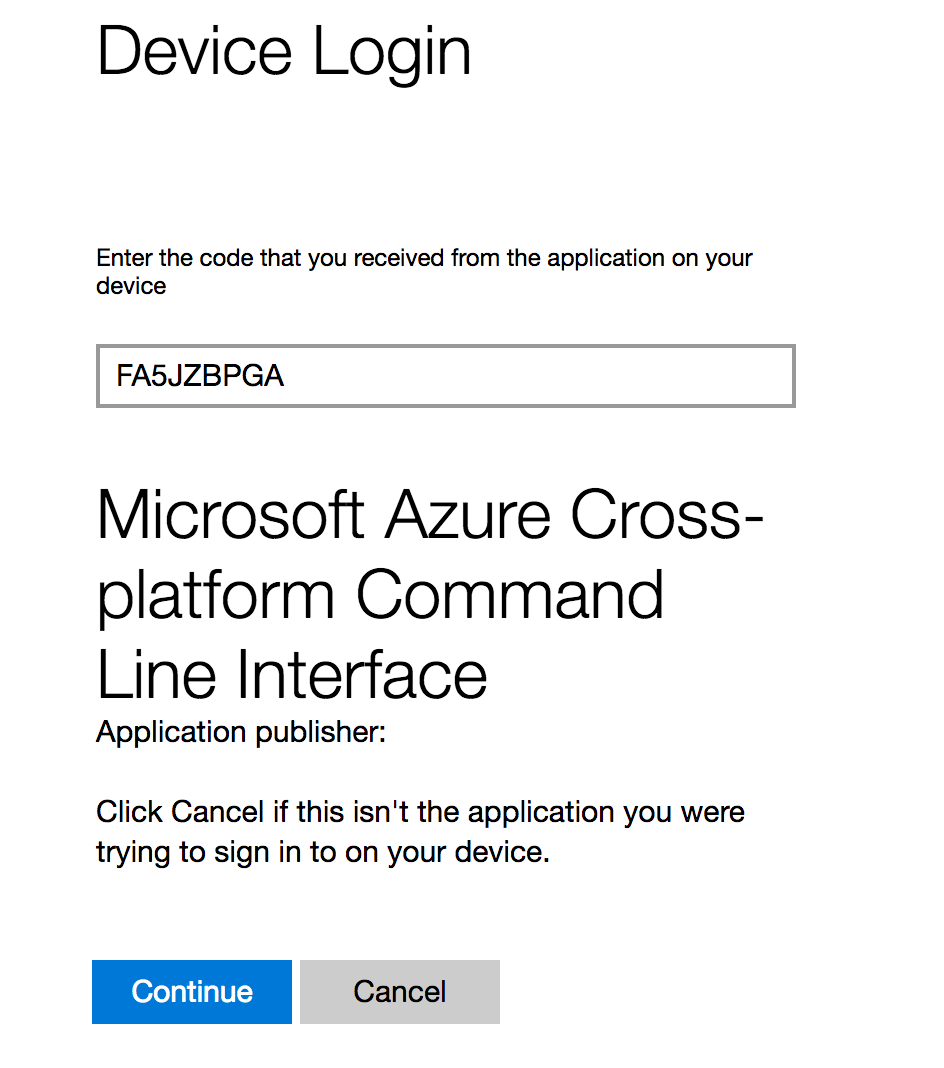
\includegraphics{imgs/azlogin.png}
\caption{}
\end{figure}

Once you're logged into your account, you can list all the Azure
subscriptions assoicated with your account by running
\texttt{az\ account\ list}, and the one you're currently defaulting to
using \texttt{az\ account\ show}:

\begin{Shaded}
\begin{Highlighting}[]
\ExtensionTok{alizaidi@MININT-C510VH5}\NormalTok{:~$ az account show}
\KeywordTok{\{}
  \StringTok{"environmentName"}\NormalTok{: }\StringTok{"AzureCloud"}\NormalTok{,}
  \StringTok{"id"}\NormalTok{: }\StringTok{"please-dont-steal-my-acount"}\NormalTok{,}
  \StringTok{"isDefault"}\NormalTok{: }\FunctionTok{true}\NormalTok{,}
  \StringTok{"name"}\NormalTok{: }\StringTok{"Not for you"}\NormalTok{,}
  \StringTok{"state"}\NormalTok{: }\StringTok{"Enabled"}\NormalTok{,}
  \StringTok{"tenantId"}\NormalTok{: }\StringTok{"nah"}\NormalTok{,}
  \StringTok{"user"}\NormalTok{: }\KeywordTok{\{}
    \StringTok{"name"}\NormalTok{: }\StringTok{"alizaidi@microsoft.com"}\NormalTok{,}
    \StringTok{"type"}\NormalTok{: }\StringTok{"user"}
  \KeywordTok{\}}
\KeywordTok{\}}
\ExtensionTok{alizaidi@MININT-C510VH5}\NormalTok{:~$ az account list}
\BuiltInTok{[}
\NormalTok{  \{}
    \StringTok{"cloudName"}\NormalTok{: }\StringTok{"AzureCloud"}\NormalTok{,}
    \StringTok{"id"}\NormalTok{: }\StringTok{"please-dont-steal-my-acount"}\NormalTok{,}
    \StringTok{"isDefault"}\NormalTok{: true,}
    \StringTok{"name"}\NormalTok{: }\StringTok{"Not for you"}\NormalTok{,}
    \StringTok{"state"}\NormalTok{: }\StringTok{"Enabled"}\NormalTok{,}
    \StringTok{"tenantId"}\NormalTok{: }\StringTok{"nah"}\NormalTok{,}
    \StringTok{"user"}\NormalTok{: \{}
      \StringTok{"name"}\NormalTok{: }\StringTok{"alizaidi@microsoft.com"}\NormalTok{,}
      \StringTok{"type"}\NormalTok{: }\StringTok{"user"}
\NormalTok{    \}}
\NormalTok{  \}}
\BuiltInTok{]}
\end{Highlighting}
\end{Shaded}

You can use the option \texttt{-\/-output\ table} to print the output in
a tabular format.

\section{Deploying with a Custom
Script}\label{deploying-with-a-custom-script}

Rather than doing this manually, I have created a custom script that
will create the DSVM for you, and also run some configuration settings
on your VM's network to allow for easier access.

You can simply deploy the DSVM by navigating to the
\texttt{labs/0-dsvm-deploy-script} directory and running

\begin{Shaded}
\begin{Highlighting}[]
\ExtensionTok{alizaidi}\NormalTok{:$ ./deploydsvm.sh}
\end{Highlighting}
\end{Shaded}

The default parameters will use your bash username as your username for
the VM, and a simple password. Feel free to change these by specThis
will create your virtual machine, open up all the necessary ports on
your VM's network security group, and save the credentials in a text
file \texttt{creds.txt}.

\section{Updating DSVM OS Disk Size}\label{updating-dsvm-os-disk-size}

By default, your primary partition on the DSVM is only 50 GBs.
Fortunately, expanding it is pretty easy. Let's again use two helper
scripts I created to make this process trivally easy. Using the
\texttt{\$VMNAME} and \texttt{\$RG} values saved in the file
\texttt{creds.txt}, fill in the following command:

\begin{Shaded}
\begin{Highlighting}[]
\ExtensionTok{expand-osdisk.sh} \StringTok{"os-size-in-GB"} \StringTok{"RG"} \StringTok{"VMNAME"}
\end{Highlighting}
\end{Shaded}

For example, I'd run

\begin{Shaded}
\begin{Highlighting}[]
\ExtensionTok{expand-disk.sh}\NormalTok{ 200 azaididlclass azaididsvm}
\end{Highlighting}
\end{Shaded}

Now you're ready to log into your VM and have some fun!

\section{\texorpdfstring{Deploying Manually \textbf{(Only Proceed if You
Didn't Use the Script
Above!)}}{Deploying Manually (Only Proceed if You Didn't Use the Script Above!)}}\label{deploying-manually-only-proceed-if-you-didnt-use-the-script-above}

If you didn't use the scripts above, I've written out the instructions
manually below.

\subsection{Create a New Resource
Group}\label{create-a-new-resource-group}

Resource groups are a convenient way of consolidating related resources
together. This is particularly handy when you have a project that will
require a variety of Azure resources and you'd like to see them all in
one-place.

Please make sure your resource group is in ``East US'' region (you could
potentially use South Central US).

In this example, I'll create a resource group called \texttt{azteachdl}
in \texttt{eastus}

\begin{Shaded}
\begin{Highlighting}[]
\ExtensionTok{alizaidi}\NormalTok{:$ az group create -n azteachdl -l eastus}
\KeywordTok{\{}
  \StringTok{"id"}\NormalTok{: }\StringTok{"/subscriptions/stay-away-from me/resourceGroups/azteachdl"}\NormalTok{,}
  \StringTok{"location"}\NormalTok{: }\StringTok{"eastus"}\NormalTok{,}
  \CommentTok{#"managedBy": null,}
  \StringTok{"name"}\NormalTok{: }\StringTok{"azteachdl"}\NormalTok{,}
  \StringTok{"properties"}\NormalTok{: }\KeywordTok{\{}
    \StringTok{"provisioningState"}\NormalTok{: }\StringTok{"Succeeded"}
  \KeywordTok{\}}\NormalTok{,}
  \StringTok{"tags"}\NormalTok{: }\ExtensionTok{null}
\KeywordTok{\}}
\end{Highlighting}
\end{Shaded}

\subsection{Create Your DSVM}\label{create-your-dsvm}

Now let's create the Linux DSVM. Edit the parameters below with your
configurations. In particular, you'll need to specify your own
\texttt{resource-group} name, a name for the data science virtual
machine, and your username.

\begin{Shaded}
\begin{Highlighting}[]
\ExtensionTok{az}\NormalTok{ vm create \textbackslash{}}
\NormalTok{    --resource-group azteachdl \textbackslash{}}
\NormalTok{    --name azdsvmclass \textbackslash{}}
\NormalTok{    --admin-username alizaidi \textbackslash{}}
\NormalTok{    --public-ip-address-dns-name algoclass \textbackslash{}}
\NormalTok{    --image microsoft-ads:linux-data-science-vm-ubuntu:linuxdsvmubuntu:latest \textbackslash{}}
\NormalTok{    --size Standard_NC6 \textbackslash{}}
\NormalTok{    --generate-ssh-keys}
\end{Highlighting}
\end{Shaded}

While the resources are being deployed, you will see a
\emph{``Running''} message displayed in your terminal. Upon completion,
you should see an output JSON table with information about your
resources:

\begin{Shaded}
\begin{Highlighting}[]
\KeywordTok{\{}
  \StringTok{"fqdns"}\NormalTok{: }\StringTok{""}\NormalTok{,}
  \StringTok{"id"}\NormalTok{: }\StringTok{"/subscriptions/keep-away/resourceGroups/azaididlclass/providers/Microsoft.Compute/virtualMachines/azaidi"}\NormalTok{,}
  \StringTok{"location"}\NormalTok{: }\StringTok{"eastus"}\NormalTok{,}
  \StringTok{"macAddress"}\NormalTok{: }\StringTok{"00-0D-3A-1B-59-48"}\NormalTok{,}
  \StringTok{"powerState"}\NormalTok{: }\StringTok{"VM running"}\NormalTok{,}
  \StringTok{"privateIpAddress"}\NormalTok{: }\StringTok{"10.0.0.4"}\NormalTok{,}
  \StringTok{"publicIpAddress"}\NormalTok{: }\StringTok{"13.00.000.000"}\NormalTok{,}
  \StringTok{"resourceGroup"}\NormalTok{: }\StringTok{"azaididlclass"}
\KeywordTok{\}}
\end{Highlighting}
\end{Shaded}

\subsection{Create a Password for the
User}\label{create-a-password-for-the-user}

In the scripted solution, the authentication is done through a password.

In the manual setup we showed how you could create a virtual machine
using the \texttt{generate-ssh-keys} option, which authenticates using
SSH keys, which by default are saved as a pair of private and public
keys in \texttt{\textasciitilde{}/.ssh/id\_rsa} and
\texttt{\textasciitilde{}/.ssh/id\_rsa.pub}. In order to access certain
web applications like Jupyter, we'll need a password for our user.

To create a password for the user, run the following:

\begin{Shaded}
\begin{Highlighting}[]
\FunctionTok{sudo}\NormalTok{ passwd }\VariableTok{$USERNAME}
\end{Highlighting}
\end{Shaded}

where \texttt{\$USERNAME} is the username you used to create the VM.

You can now navigate to the portal and check for your resources.

\chapter{Upgrading CNTK and CUDNN}\label{upgrading-cntk-and-cudnn}

In this lab, we'll upgrade from CNTK version 2.0 to CNTK 2.2.

\section{Updating CNTK}\label{updating-cntk}

CNTK is available in a variety of
\href{https://docs.microsoft.com/en-us/cognitive-toolkit/setup-cntk-on-your-machine}{precompiled
binaries}, which you can install using the \texttt{pip} installer.

\section{Updating CNTK With a Single
Script}\label{updating-cntk-with-a-single-script}

I've created a single script to make the upgrade process a lot simper:

\begin{Shaded}
\begin{Highlighting}[]
\ExtensionTok{./cntk-install.sh}
\end{Highlighting}
\end{Shaded}

This will create a new \texttt{conda\ environment} called
\texttt{cntk-py35} with your new CNTK installation.

\subsection{Launch JupyterLab}\label{launch-jupyterlab}

JupyterLab is an updated environment based on Jupyter. In addition to
the notebooks popularized by Jupyter, JupyterLab has an inspector for
viewing help files quickly, a terminal, and a file browser. This makes
for a more complete interactive development experience!

To launch JupyterLab and keep it running, I recommend first creating a
password you can use to log into your server without having to use
special tokens (see the documentation
\href{http://nbconvert.readthedocs.io/en/latest/usage.html}{here}.
Moreover, since we want to keep JupyterLab running in the background
even after we close out our terminal session, I'd recommend using
\href{https://github.com/tmux/tmux/wiki}{tmux} to launch your Jupyter
session.

\begin{Shaded}
\begin{Highlighting}[]

\ExtensionTok{tmux}\NormalTok{ new -s jupyterlab}
\ExtensionTok{jupyter}\NormalTok{ notebook --generate-config}
\ExtensionTok{jupyter}\NormalTok{ notebook password}
\ExtensionTok{jupyter}\NormalTok{ lab --ip=}\StringTok{"*"} 
\ExtensionTok{tmux}\NormalTok{ detach}
\ExtensionTok{jupyter}\NormalTok{ notebook list}
\end{Highlighting}
\end{Shaded}

Now navigate to your :8888 to interact with JupyterLab!

\section{\texorpdfstring{Manually Updating CNTK and Launching Jupyter
(\textbf{No Need to Do This if You Use the
Script})}{Manually Updating CNTK and Launching Jupyter (No Need to Do This if You Use the Script)}}\label{manually-updating-cntk-and-launching-jupyter-no-need-to-do-this-if-you-use-the-script}

Only follow the steps below if the script above didn't work or if you
like doing this manually\ldots{}

\subsection{Create Conda Virtual
Environment}\label{create-conda-virtual-environment}

For this tutorial, we'll use the
\href{https://conda.io/docs/using/envs.html}{\texttt{conda} virtual
environment manager} to create and modify Python virtual environments.
You can create a Python 3.5 environment with \texttt{conda} by using the
\texttt{conda\ create} command:

\begin{Shaded}
\begin{Highlighting}[]
\ExtensionTok{conda}\NormalTok{ create -n cntk-py35 python=3.5 anaconda}
\end{Highlighting}
\end{Shaded}

The environment will be named \texttt{cntk-py35} and the additional flag
\texttt{anaconda} ensures that the distribution will install over a 100
prebuilt Python packages for scientific computing (list
\href{https://docs.continuum.io/anaconda/packages/pkg-docs}{here}).

\subsection{\texorpdfstring{Install CNTK Using \texttt{pip} Binary
Wheels}{Install CNTK Using pip Binary Wheels}}\label{install-cntk-using-pip-binary-wheels}

We can activate that environment by running

\begin{Shaded}
\begin{Highlighting}[]
\BuiltInTok{source}\NormalTok{ activate cntk-py35}
\end{Highlighting}
\end{Shaded}

Now that we are in our virutla environment for CNTK, let's install the
\href{https://docs.microsoft.com/en-us/cognitive-toolkit/setup-linux-python?tabs=cntkpy21}{appropriate
Python binary} using a Python ``wheel''. For example, here are the
installation instructions for CNTK on a Python 3.5 environment with
Ubuntu 16.04 system with GPU support:

\begin{Shaded}
\begin{Highlighting}[]
\ExtensionTok{pip}\NormalTok{ install https://cntk.ai/PythonWheel/GPU/cntk-2.1-cp35-cp35m-linux_x86_64.whl}
\end{Highlighting}
\end{Shaded}

\subsection{Temporary Fixes}\label{temporary-fixes}

Let's take complete ownership of our \texttt{home} and \texttt{anaconda}
directories:

\begin{Shaded}
\begin{Highlighting}[]
\FunctionTok{sudo}\NormalTok{ chown alizaidi:alizaidi -R /home/alizaidi}
\BuiltInTok{source}\NormalTok{ deactivate}
\FunctionTok{sudo}\NormalTok{ chown alizaidi:alizaidi -R /anaconda/}
\ExtensionTok{pip}\NormalTok{ install -U pip}
\end{Highlighting}
\end{Shaded}

\textbf{IMPORTANT} replace \texttt{alizaidi} with the username you used
to create the DSVM.

Update \texttt{ipython} and related packages:

\begin{Shaded}
\begin{Highlighting}[]
\ExtensionTok{pip}\NormalTok{ install --upgrade --force-reinstall jupyter}
\end{Highlighting}
\end{Shaded}

Remove \texttt{az\_ml\_magic} from ipython startup:

\begin{Shaded}
\begin{Highlighting}[]
\FunctionTok{rm}\NormalTok{ ~/.ipython/profile_default/startup/az_ml_magic.py}
\end{Highlighting}
\end{Shaded}

\subsection{Conda Extensions}\label{conda-extensions}

Since we created a new environment, let's also install some extensions
that will make it easier to find that environment from JupyterHub.

\begin{Shaded}
\begin{Highlighting}[]
\ExtensionTok{conda}\NormalTok{ install nb_conda}
\ExtensionTok{conda}\NormalTok{ install ipykernel}
\ExtensionTok{python}\NormalTok{ -m ipykernel install --user --name cntk-py35 --display-name }\StringTok{"cntk-py35"}
\ExtensionTok{jupyter}\NormalTok{ kernelspec list}
\end{Highlighting}
\end{Shaded}

\subsection{Install Keras}\label{install-keras}

Let's also install Keras in this specific Python environment

\begin{Shaded}
\begin{Highlighting}[]
\BuiltInTok{source}\NormalTok{ activate cntk-py35}
\ExtensionTok{pip}\NormalTok{ install keras}
\end{Highlighting}
\end{Shaded}

\chapter{Transfer Learning with CNTK}\label{transfer-learning-with-cntk}

\section{Classifying Dogs and Cats Using a Pre-Trained
Network}\label{classifying-dogs-and-cats-using-a-pre-trained-network}

This notebook provides a walkthrough of how to use an existing model,
trained on a large corpus of images, and retrain it on a narrower class
of images for a specific domain. In particular, we will be looking at
the famous Kaggle competition,
\href{https://www.kaggle.com/c/dogs-vs-cats-redux-kernels-edition}{Cats
vs.~Dogs}.

Let's import our core scientific python modules, \texttt{numpy},
\texttt{matplotlib} and \texttt{pandas}. In addition, we import
\texttt{CNTK}. If you have trouble getting \texttt{CNTK} to run on a GPU
(and you're sure you have one properly installed), you can manually
request CNTK use the \texttt{gpu} device by commenting out the line
after the import.

We have some helper functions in the \texttt{utils.py} script that we'll
use to download our pre-trained network from a repository.

\begin{Shaded}
\begin{Highlighting}[]
\ImportTok{import}\NormalTok{ os, cv2, random}
\ImportTok{import}\NormalTok{ numpy }\ImportTok{as}\NormalTok{ np}
\ImportTok{import}\NormalTok{ os, shutil}
\ImportTok{import}\NormalTok{ random}
\ImportTok{from}\NormalTok{ glob }\ImportTok{import}\NormalTok{ glob}
\NormalTok{np.random.seed(}\DecValTok{123}\NormalTok{)}
\ImportTok{import}\NormalTok{ matplotlib.pyplot }\ImportTok{as}\NormalTok{ plt}
\ImportTok{from}\NormalTok{ matplotlib }\ImportTok{import}\NormalTok{ ticker}
\ImportTok{import}\NormalTok{ matplotlib.image }\ImportTok{as}\NormalTok{ mpimg}
\ImportTok{import}\NormalTok{ seaborn }\ImportTok{as}\NormalTok{ sns}
\ImportTok{import}\NormalTok{ itertools}
\ImportTok{import}\NormalTok{ pandas }\ImportTok{as}\NormalTok{ pd}
\NormalTok{sns.}\BuiltInTok{set}\NormalTok{(style}\OperatorTok{=}\StringTok{"white"}\NormalTok{)}
\OperatorTok{%}\NormalTok{matplotlib inline}



\ImportTok{import}\NormalTok{ cntk }\ImportTok{as}\NormalTok{ C}
\CommentTok{# C.device.try_set_default_device(C.device.gpu(0))}
\ImportTok{import}\NormalTok{ cntk.io.transforms }\ImportTok{as}\NormalTok{ xforms}

\ImportTok{from}\NormalTok{ __future__ }\ImportTok{import}\NormalTok{ print_function}
\ImportTok{from}\NormalTok{ utils.download_model }\ImportTok{import}\NormalTok{ models, download_model_by_name, list_available_models}
\ImportTok{from}\NormalTok{ PIL }\ImportTok{import}\NormalTok{ Image}
\ImportTok{from}\NormalTok{ IPython.display }\ImportTok{import}\NormalTok{ display, SVG}
\OperatorTok{%}\NormalTok{load_ext autoreload}
\end{Highlighting}
\end{Shaded}

\subsection{Download Data}\label{download-data}

One of the easiest ways to download data from Kaggle competitions is
using the \href{https://github.com/floydwch/kaggle-cli}{kaggle-cli}.

\begin{verbatim}
kg download -u <username> -p <password> -c dogs-vs-cats-redux-kernels-edition
\end{verbatim}

For now, you can download the data just by running the bash commands
below, which will download the data from my public blob storage account.
Note, the data set is \textasciitilde{}815 MB in size, and is in a
storage container in \emph{Central US}.

\begin{Shaded}
\begin{Highlighting}[]
\ExtensionTok{%%bash}
\FunctionTok{wget}\NormalTok{ -q https://alizaidi.blob.core.windows.net/training/catsdogs/data.zip}
\FunctionTok{unzip}\NormalTok{ data.zip}
\BuiltInTok{cd}\NormalTok{ data}
\FunctionTok{unzip}\NormalTok{ *.zip}
\FunctionTok{rm}\NormalTok{ ../data.zip}
\end{Highlighting}
\end{Shaded}

\section{Create Train, Test and Validate
Sets}\label{create-train-test-and-validate-sets}

Our data arrives in a rather simple structure:

\begin{verbatim}
    train/
        cat.****.jpg
        dog.****.jpg
    test/
        *****.jpg
\end{verbatim}

In order to evaluate our model (especially if we are tinkering with
hyperparameters), it is important we separate a portion of our train set
and use that for evaluation/validation. You shouldn't use your test set
to guide your choice of hyperparameters, as this will likely lead to
overfitted networks.

The function below takes a 20\% sample from the \texttt{train} directory
and puts it in a new directory called \texttt{val}. It leaves the
\texttt{data/train} directory completely untouched, and instead makes a
fully copy to \texttt{./train} from where it takes the sample and moves
it to \texttt{./val}.

\begin{Shaded}
\begin{Highlighting}[]
\KeywordTok{def}\NormalTok{ train_val_split(train_path, split_train_path, split_val_path):}
    
    \ControlFlowTok{if}\NormalTok{(os.path.exists(split_train_path)): shutil.rmtree(split_train_path)}

\NormalTok{    os.mkdir(split_val_path)}

    \CommentTok{# Next copy everything in the combined training directory to the split training directory}
\NormalTok{    shutil.copytree(train_path, split_train_path)}

\NormalTok{    num_folds }\OperatorTok{=} \DecValTok{5}  \CommentTok{# One of the folds to be val, the rest for train...}

    \ControlFlowTok{for}\NormalTok{ subdir }\KeywordTok{in}\NormalTok{ glob(split_train_path }\OperatorTok{+} \StringTok{'*'}\NormalTok{):}
\NormalTok{        g }\OperatorTok{=}\NormalTok{ glob(subdir }\OperatorTok{+} \StringTok{'/*.jpg'}\NormalTok{)}
\NormalTok{        shuf }\OperatorTok{=}\NormalTok{ np.random.permutation(g)}
        \ControlFlowTok{for}\NormalTok{ i }\KeywordTok{in} \BuiltInTok{range}\NormalTok{(}\BuiltInTok{int}\NormalTok{(}\BuiltInTok{round}\NormalTok{(}\BuiltInTok{len}\NormalTok{(shuf)}\OperatorTok{/}\NormalTok{num_folds))):}
            \BuiltInTok{print}\NormalTok{(}\StringTok{"Transferring "}\NormalTok{, shuf[i], }\StringTok{" to "}\NormalTok{, }
\NormalTok{                  split_val_path }\OperatorTok{+} \StringTok{"/"} \OperatorTok{+}\NormalTok{ shuf[i].split(}\StringTok{'/'}\NormalTok{)[}\DecValTok{2}\NormalTok{])}
\NormalTok{            os.rename(shuf[i], split_val_path }\OperatorTok{+} \StringTok{"/"} \OperatorTok{+}\NormalTok{ shuf[i].split(}\StringTok{'/'}\NormalTok{)[}\DecValTok{2}\NormalTok{])}
\end{Highlighting}
\end{Shaded}

\begin{Shaded}
\begin{Highlighting}[]
\NormalTok{train_val_split(train_path }\OperatorTok{=} \StringTok{"data/train"}\NormalTok{, split_train_path}\OperatorTok{=}\StringTok{"./train"}\NormalTok{, split_val_path}\OperatorTok{=}\StringTok{"./val"}\NormalTok{)}
\end{Highlighting}
\end{Shaded}

\begin{verbatim}
Transferring  ./train/cat.6109.jpg  to  ./val/cat.6109.jpg
Transferring  ./train/dog.5873.jpg  to  ./val/dog.5873.jpg
Transferring  ./train/dog.9468.jpg  to  ./val/dog.9468.jpg
Transferring  ./train/cat.9550.jpg  to  ./val/cat.9550.jpg
Transferring  ./train/dog.111.jpg  to  ./val/dog.111.jpg
Transferring  ./train/cat.2628.jpg  to  ./val/cat.2628.jpg
Transferring  ./train/dog.6430.jpg  to  ./val/dog.6430.jpg
Transferring  ./train/dog.642.jpg  to  ./val/dog.642.jpg
Transferring  ./train/dog.9465.jpg  to  ./val/dog.9465.jpg
Transferring  ./train/dog.10947.jpg  to  ./val/dog.10947.jpg
Transferring  ./train/cat.10475.jpg  to  ./val/cat.10475.jpg
Transferring  ./train/dog.6433.jpg  to  ./val/dog.6433.jpg
Transferring  ./train/cat.5853.jpg  to  ./val/cat.5853.jpg
Transferring  ./train/cat.10527.jpg  to  ./val/cat.10527.jpg
Transferring  ./train/cat.11977.jpg  to  ./val/cat.11977.jpg
Transferring  ./train/dog.5173.jpg  to  ./val/dog.5173.jpg
Transferring  ./train/cat.9391.jpg  to  ./val/cat.9391.jpg
Transferring  ./train/cat.3189.jpg  to  ./val/cat.3189.jpg
Transferring  ./train/dog.4299.jpg  to  ./val/dog.4299.jpg
Transferring  ./train/dog.11492.jpg  to  ./val/dog.11492.jpg
Transferring  ./train/dog.10894.jpg  to  ./val/dog.10894.jpg
Transferring  ./train/cat.2177.jpg  to  ./val/cat.2177.jpg
Transferring  ./train/cat.9712.jpg  to  ./val/cat.9712.jpg
Transferring  ./train/cat.5060.jpg  to  ./val/cat.5060.jpg
Transferring  ./train/cat.8942.jpg  to  ./val/cat.8942.jpg
Transferring  ./train/cat.3977.jpg  to  ./val/cat.3977.jpg
Transferring  ./train/cat.6462.jpg  to  ./val/cat.6462.jpg
Transferring  ./train/dog.8681.jpg  to  ./val/dog.8681.jpg
Transferring  ./train/dog.6768.jpg  to  ./val/dog.6768.jpg
Transferring  ./train/dog.11025.jpg  to  ./val/dog.11025.jpg
Transferring  ./train/cat.895.jpg  to  ./val/cat.895.jpg
Transferring  ./train/dog.5775.jpg  to  ./val/dog.5775.jpg
Transferring  ./train/cat.5206.jpg  to  ./val/cat.5206.jpg
Transferring  ./train/cat.7135.jpg  to  ./val/cat.7135.jpg
Transferring  ./train/cat.5365.jpg  to  ./val/cat.5365.jpg
Transferring  ./train/cat.5888.jpg  to  ./val/cat.5888.jpg
Transferring  ./train/cat.11863.jpg  to  ./val/cat.11863.jpg
Transferring  ./train/cat.44.jpg  to  ./val/cat.44.jpg
Transferring  ./train/dog.8802.jpg  to  ./val/dog.8802.jpg
Transferring  ./train/cat.5389.jpg  to  ./val/cat.5389.jpg
Transferring  ./train/cat.1922.jpg  to  ./val/cat.1922.jpg
Transferring  ./train/cat.11303.jpg  to  ./val/cat.11303.jpg
Transferring  ./train/dog.7221.jpg  to  ./val/dog.7221.jpg
Transferring  ./train/dog.10890.jpg  to  ./val/dog.10890.jpg
Transferring  ./train/cat.12050.jpg  to  ./val/cat.12050.jpg
Transferring  ./train/dog.1726.jpg  to  ./val/dog.1726.jpg
Transferring  ./train/dog.1230.jpg  to  ./val/dog.1230.jpg
Transferring  ./train/dog.10810.jpg  to  ./val/dog.10810.jpg
Transferring  ./train/cat.11925.jpg  to  ./val/cat.11925.jpg
Transferring  ./train/dog.4675.jpg  to  ./val/dog.4675.jpg
Transferring  ./train/cat.7273.jpg  to  ./val/cat.7273.jpg
Transferring  ./train/cat.4016.jpg  to  ./val/cat.4016.jpg
Transferring  ./train/cat.10264.jpg  to  ./val/cat.10264.jpg
Transferring  ./train/dog.2864.jpg  to  ./val/dog.2864.jpg
Transferring  ./train/cat.8417.jpg  to  ./val/cat.8417.jpg
Transferring  ./train/dog.11487.jpg  to  ./val/dog.11487.jpg
Transferring  ./train/cat.3400.jpg  to  ./val/cat.3400.jpg
Transferring  ./train/dog.7898.jpg  to  ./val/dog.7898.jpg
Transferring  ./train/dog.53.jpg  to  ./val/dog.53.jpg
Transferring  ./train/dog.3764.jpg  to  ./val/dog.3764.jpg
Transferring  ./train/dog.466.jpg  to  ./val/dog.466.jpg
Transferring  ./train/dog.3664.jpg  to  ./val/dog.3664.jpg
Transferring  ./train/dog.4542.jpg  to  ./val/dog.4542.jpg
Transferring  ./train/cat.40.jpg  to  ./val/cat.40.jpg
Transferring  ./train/dog.828.jpg  to  ./val/dog.828.jpg
Transferring  ./train/cat.4011.jpg  to  ./val/cat.4011.jpg
Transferring  ./train/dog.4882.jpg  to  ./val/dog.4882.jpg
Transferring  ./train/dog.10431.jpg  to  ./val/dog.10431.jpg
Transferring  ./train/cat.11108.jpg  to  ./val/cat.11108.jpg
Transferring  ./train/dog.9434.jpg  to  ./val/dog.9434.jpg
Transferring  ./train/cat.10261.jpg  to  ./val/cat.10261.jpg
Transferring  ./train/dog.5239.jpg  to  ./val/dog.5239.jpg
Transferring  ./train/dog.10800.jpg  to  ./val/dog.10800.jpg
Transferring  ./train/dog.6166.jpg  to  ./val/dog.6166.jpg
Transferring  ./train/cat.3282.jpg  to  ./val/cat.3282.jpg
Transferring  ./train/dog.5340.jpg  to  ./val/dog.5340.jpg
Transferring  ./train/dog.381.jpg  to  ./val/dog.381.jpg
Transferring  ./train/cat.7004.jpg  to  ./val/cat.7004.jpg
Transferring  ./train/cat.916.jpg  to  ./val/cat.916.jpg
Transferring  ./train/cat.897.jpg  to  ./val/cat.897.jpg
Transferring  ./train/dog.11691.jpg  to  ./val/dog.11691.jpg
Transferring  ./train/dog.7296.jpg  to  ./val/dog.7296.jpg
Transferring  ./train/dog.10832.jpg  to  ./val/dog.10832.jpg
Transferring  ./train/dog.8954.jpg  to  ./val/dog.8954.jpg
Transferring  ./train/dog.3381.jpg  to  ./val/dog.3381.jpg
Transferring  ./train/cat.6213.jpg  to  ./val/cat.6213.jpg
Transferring  ./train/dog.398.jpg  to  ./val/dog.398.jpg
Transferring  ./train/dog.10766.jpg  to  ./val/dog.10766.jpg
Transferring  ./train/cat.2180.jpg  to  ./val/cat.2180.jpg
Transferring  ./train/dog.1537.jpg  to  ./val/dog.1537.jpg
Transferring  ./train/dog.1839.jpg  to  ./val/dog.1839.jpg
Transferring  ./train/cat.11616.jpg  to  ./val/cat.11616.jpg
Transferring  ./train/dog.8059.jpg  to  ./val/dog.8059.jpg
Transferring  ./train/cat.3159.jpg  to  ./val/cat.3159.jpg
Transferring  ./train/cat.4862.jpg  to  ./val/cat.4862.jpg
Transferring  ./train/cat.5172.jpg  to  ./val/cat.5172.jpg
Transferring  ./train/dog.8022.jpg  to  ./val/dog.8022.jpg
Transferring  ./train/cat.1158.jpg  to  ./val/cat.1158.jpg
Transferring  ./train/cat.8352.jpg  to  ./val/cat.8352.jpg
Transferring  ./train/cat.11530.jpg  to  ./val/cat.11530.jpg
Transferring  ./train/cat.3688.jpg  to  ./val/cat.3688.jpg
Transferring  ./train/cat.10355.jpg  to  ./val/cat.10355.jpg
Transferring  ./train/cat.9971.jpg  to  ./val/cat.9971.jpg
Transferring  ./train/dog.9724.jpg  to  ./val/dog.9724.jpg
Transferring  ./train/dog.2813.jpg  to  ./val/dog.2813.jpg
Transferring  ./train/dog.2437.jpg  to  ./val/dog.2437.jpg
Transferring  ./train/dog.10684.jpg  to  ./val/dog.10684.jpg
Transferring  ./train/cat.12494.jpg  to  ./val/cat.12494.jpg
Transferring  ./train/dog.10339.jpg  to  ./val/dog.10339.jpg
Transferring  ./train/cat.1893.jpg  to  ./val/cat.1893.jpg
Transferring  ./train/cat.10846.jpg  to  ./val/cat.10846.jpg
Transferring  ./train/cat.2889.jpg  to  ./val/cat.2889.jpg
Transferring  ./train/cat.4383.jpg  to  ./val/cat.4383.jpg
Transferring  ./train/dog.1421.jpg  to  ./val/dog.1421.jpg
Transferring  ./train/dog.3127.jpg  to  ./val/dog.3127.jpg
Transferring  ./train/cat.11644.jpg  to  ./val/cat.11644.jpg
Transferring  ./train/dog.10964.jpg  to  ./val/dog.10964.jpg
Transferring  ./train/dog.11113.jpg  to  ./val/dog.11113.jpg
Transferring  ./train/dog.2329.jpg  to  ./val/dog.2329.jpg
Transferring  ./train/dog.2564.jpg  to  ./val/dog.2564.jpg
Transferring  ./train/cat.4963.jpg  to  ./val/cat.4963.jpg
Transferring  ./train/cat.11001.jpg  to  ./val/cat.11001.jpg
Transferring  ./train/dog.10935.jpg  to  ./val/dog.10935.jpg
Transferring  ./train/cat.7498.jpg  to  ./val/cat.7498.jpg
Transferring  ./train/dog.9226.jpg  to  ./val/dog.9226.jpg
Transferring  ./train/cat.3944.jpg  to  ./val/cat.3944.jpg
Transferring  ./train/cat.7497.jpg  to  ./val/cat.7497.jpg
Transferring  ./train/cat.7279.jpg  to  ./val/cat.7279.jpg
Transferring  ./train/cat.2195.jpg  to  ./val/cat.2195.jpg
Transferring  ./train/cat.3879.jpg  to  ./val/cat.3879.jpg
Transferring  ./train/cat.10792.jpg  to  ./val/cat.10792.jpg
Transferring  ./train/dog.8830.jpg  to  ./val/dog.8830.jpg
Transferring  ./train/cat.8696.jpg  to  ./val/cat.8696.jpg
Transferring  ./train/cat.5368.jpg  to  ./val/cat.5368.jpg
Transferring  ./train/cat.11236.jpg  to  ./val/cat.11236.jpg
Transferring  ./train/cat.11912.jpg  to  ./val/cat.11912.jpg
Transferring  ./train/dog.7700.jpg  to  ./val/dog.7700.jpg
Transferring  ./train/cat.5559.jpg  to  ./val/cat.5559.jpg
Transferring  ./train/dog.7368.jpg  to  ./val/dog.7368.jpg
Transferring  ./train/cat.431.jpg  to  ./val/cat.431.jpg
Transferring  ./train/cat.3290.jpg  to  ./val/cat.3290.jpg
Transferring  ./train/cat.48.jpg  to  ./val/cat.48.jpg
Transferring  ./train/cat.11127.jpg  to  ./val/cat.11127.jpg
Transferring  ./train/cat.10196.jpg  to  ./val/cat.10196.jpg
Transferring  ./train/dog.7490.jpg  to  ./val/dog.7490.jpg
Transferring  ./train/cat.5385.jpg  to  ./val/cat.5385.jpg
Transferring  ./train/cat.1743.jpg  to  ./val/cat.1743.jpg
Transferring  ./train/cat.318.jpg  to  ./val/cat.318.jpg
Transferring  ./train/dog.9052.jpg  to  ./val/dog.9052.jpg
Transferring  ./train/cat.9702.jpg  to  ./val/cat.9702.jpg
Transferring  ./train/dog.10308.jpg  to  ./val/dog.10308.jpg
Transferring  ./train/cat.10796.jpg  to  ./val/cat.10796.jpg
Transferring  ./train/dog.8611.jpg  to  ./val/dog.8611.jpg
Transferring  ./train/dog.11436.jpg  to  ./val/dog.11436.jpg
Transferring  ./train/dog.6472.jpg  to  ./val/dog.6472.jpg
Transferring  ./train/dog.3.jpg  to  ./val/dog.3.jpg
Transferring  ./train/cat.3435.jpg  to  ./val/cat.3435.jpg
Transferring  ./train/cat.9510.jpg  to  ./val/cat.9510.jpg
Transferring  ./train/dog.1089.jpg  to  ./val/dog.1089.jpg
Transferring  ./train/cat.3774.jpg  to  ./val/cat.3774.jpg
Transferring  ./train/cat.7718.jpg  to  ./val/cat.7718.jpg
Transferring  ./train/dog.8241.jpg  to  ./val/dog.8241.jpg
Transferring  ./train/cat.176.jpg  to  ./val/cat.176.jpg
Transferring  ./train/cat.9290.jpg  to  ./val/cat.9290.jpg
Transferring  ./train/cat.1413.jpg  to  ./val/cat.1413.jpg
Transferring  ./train/cat.4561.jpg  to  ./val/cat.4561.jpg
Transferring  ./train/cat.7831.jpg  to  ./val/cat.7831.jpg
Transferring  ./train/cat.11532.jpg  to  ./val/cat.11532.jpg
Transferring  ./train/dog.11504.jpg  to  ./val/dog.11504.jpg
Transferring  ./train/dog.8288.jpg  to  ./val/dog.8288.jpg
Transferring  ./train/cat.4578.jpg  to  ./val/cat.4578.jpg
Transferring  ./train/cat.1411.jpg  to  ./val/cat.1411.jpg
Transferring  ./train/cat.6766.jpg  to  ./val/cat.6766.jpg
Transferring  ./train/cat.9179.jpg  to  ./val/cat.9179.jpg
Transferring  ./train/dog.451.jpg  to  ./val/dog.451.jpg
Transferring  ./train/dog.9791.jpg  to  ./val/dog.9791.jpg
Transferring  ./train/cat.3905.jpg  to  ./val/cat.3905.jpg
Transferring  ./train/cat.942.jpg  to  ./val/cat.942.jpg
Transferring  ./train/dog.6976.jpg  to  ./val/dog.6976.jpg
Transferring  ./train/dog.7236.jpg  to  ./val/dog.7236.jpg
Transferring  ./train/dog.11624.jpg  to  ./val/dog.11624.jpg
Transferring  ./train/cat.3512.jpg  to  ./val/cat.3512.jpg
Transferring  ./train/cat.2220.jpg  to  ./val/cat.2220.jpg
Transferring  ./train/dog.6570.jpg  to  ./val/dog.6570.jpg
Transferring  ./train/cat.4014.jpg  to  ./val/cat.4014.jpg
Transferring  ./train/cat.2115.jpg  to  ./val/cat.2115.jpg
Transferring  ./train/dog.10415.jpg  to  ./val/dog.10415.jpg
Transferring  ./train/cat.11755.jpg  to  ./val/cat.11755.jpg
Transferring  ./train/dog.457.jpg  to  ./val/dog.457.jpg
Transferring  ./train/cat.4713.jpg  to  ./val/cat.4713.jpg
Transferring  ./train/dog.1975.jpg  to  ./val/dog.1975.jpg
Transferring  ./train/cat.10494.jpg  to  ./val/cat.10494.jpg
Transferring  ./train/dog.9105.jpg  to  ./val/dog.9105.jpg
Transferring  ./train/dog.10218.jpg  to  ./val/dog.10218.jpg
Transferring  ./train/dog.6414.jpg  to  ./val/dog.6414.jpg
Transferring  ./train/cat.10545.jpg  to  ./val/cat.10545.jpg
Transferring  ./train/dog.12302.jpg  to  ./val/dog.12302.jpg
Transferring  ./train/dog.5343.jpg  to  ./val/dog.5343.jpg
Transferring  ./train/dog.7211.jpg  to  ./val/dog.7211.jpg
Transferring  ./train/cat.4286.jpg  to  ./val/cat.4286.jpg
Transferring  ./train/dog.557.jpg  to  ./val/dog.557.jpg
Transferring  ./train/dog.9013.jpg  to  ./val/dog.9013.jpg
Transferring  ./train/dog.3813.jpg  to  ./val/dog.3813.jpg
Transferring  ./train/cat.3246.jpg  to  ./val/cat.3246.jpg
Transferring  ./train/cat.11881.jpg  to  ./val/cat.11881.jpg
Transferring  ./train/dog.4653.jpg  to  ./val/dog.4653.jpg
Transferring  ./train/cat.2715.jpg  to  ./val/cat.2715.jpg
Transferring  ./train/cat.12233.jpg  to  ./val/cat.12233.jpg
Transferring  ./train/dog.4135.jpg  to  ./val/dog.4135.jpg
Transferring  ./train/cat.5835.jpg  to  ./val/cat.5835.jpg
Transferring  ./train/cat.5269.jpg  to  ./val/cat.5269.jpg
Transferring  ./train/cat.10502.jpg  to  ./val/cat.10502.jpg
Transferring  ./train/cat.899.jpg  to  ./val/cat.899.jpg
Transferring  ./train/cat.7836.jpg  to  ./val/cat.7836.jpg
Transferring  ./train/cat.10832.jpg  to  ./val/cat.10832.jpg
Transferring  ./train/cat.8283.jpg  to  ./val/cat.8283.jpg
Transferring  ./train/cat.523.jpg  to  ./val/cat.523.jpg
Transferring  ./train/cat.9794.jpg  to  ./val/cat.9794.jpg
Transferring  ./train/cat.4199.jpg  to  ./val/cat.4199.jpg
Transferring  ./train/dog.11449.jpg  to  ./val/dog.11449.jpg
Transferring  ./train/dog.10089.jpg  to  ./val/dog.10089.jpg
Transferring  ./train/cat.11357.jpg  to  ./val/cat.11357.jpg
Transferring  ./train/dog.11004.jpg  to  ./val/dog.11004.jpg
Transferring  ./train/cat.10761.jpg  to  ./val/cat.10761.jpg
Transferring  ./train/dog.8943.jpg  to  ./val/dog.8943.jpg
Transferring  ./train/cat.2578.jpg  to  ./val/cat.2578.jpg
Transferring  ./train/cat.4612.jpg  to  ./val/cat.4612.jpg
Transferring  ./train/cat.5747.jpg  to  ./val/cat.5747.jpg
Transferring  ./train/cat.4061.jpg  to  ./val/cat.4061.jpg
Transferring  ./train/dog.4870.jpg  to  ./val/dog.4870.jpg
Transferring  ./train/dog.9980.jpg  to  ./val/dog.9980.jpg
Transferring  ./train/dog.9308.jpg  to  ./val/dog.9308.jpg
Transferring  ./train/dog.11065.jpg  to  ./val/dog.11065.jpg
Transferring  ./train/dog.7899.jpg  to  ./val/dog.7899.jpg
Transferring  ./train/cat.2830.jpg  to  ./val/cat.2830.jpg
Transferring  ./train/cat.9828.jpg  to  ./val/cat.9828.jpg
Transferring  ./train/cat.8384.jpg  to  ./val/cat.8384.jpg
Transferring  ./train/cat.1926.jpg  to  ./val/cat.1926.jpg
Transferring  ./train/cat.11724.jpg  to  ./val/cat.11724.jpg
Transferring  ./train/cat.2630.jpg  to  ./val/cat.2630.jpg
Transferring  ./train/dog.1228.jpg  to  ./val/dog.1228.jpg
Transferring  ./train/cat.5504.jpg  to  ./val/cat.5504.jpg
Transferring  ./train/cat.11025.jpg  to  ./val/cat.11025.jpg
Transferring  ./train/cat.1710.jpg  to  ./val/cat.1710.jpg
Transferring  ./train/cat.8272.jpg  to  ./val/cat.8272.jpg
Transferring  ./train/cat.4157.jpg  to  ./val/cat.4157.jpg
Transferring  ./train/cat.7869.jpg  to  ./val/cat.7869.jpg
Transferring  ./train/dog.6671.jpg  to  ./val/dog.6671.jpg
Transferring  ./train/dog.229.jpg  to  ./val/dog.229.jpg
Transferring  ./train/dog.7978.jpg  to  ./val/dog.7978.jpg
Transferring  ./train/cat.2217.jpg  to  ./val/cat.2217.jpg
Transferring  ./train/cat.10809.jpg  to  ./val/cat.10809.jpg
Transferring  ./train/dog.5391.jpg  to  ./val/dog.5391.jpg
Transferring  ./train/dog.386.jpg  to  ./val/dog.386.jpg
Transferring  ./train/dog.12318.jpg  to  ./val/dog.12318.jpg
Transferring  ./train/cat.5586.jpg  to  ./val/cat.5586.jpg
Transferring  ./train/cat.11033.jpg  to  ./val/cat.11033.jpg
Transferring  ./train/dog.4617.jpg  to  ./val/dog.4617.jpg
Transferring  ./train/dog.10416.jpg  to  ./val/dog.10416.jpg
Transferring  ./train/cat.2950.jpg  to  ./val/cat.2950.jpg
Transferring  ./train/cat.7226.jpg  to  ./val/cat.7226.jpg
Transferring  ./train/cat.4658.jpg  to  ./val/cat.4658.jpg
Transferring  ./train/dog.4516.jpg  to  ./val/dog.4516.jpg
Transferring  ./train/cat.5340.jpg  to  ./val/cat.5340.jpg
Transferring  ./train/cat.223.jpg  to  ./val/cat.223.jpg
Transferring  ./train/dog.5236.jpg  to  ./val/dog.5236.jpg
Transferring  ./train/dog.12331.jpg  to  ./val/dog.12331.jpg
Transferring  ./train/cat.3717.jpg  to  ./val/cat.3717.jpg
Transferring  ./train/cat.6466.jpg  to  ./val/cat.6466.jpg
Transferring  ./train/cat.11389.jpg  to  ./val/cat.11389.jpg
Transferring  ./train/cat.4385.jpg  to  ./val/cat.4385.jpg
Transferring  ./train/cat.4401.jpg  to  ./val/cat.4401.jpg
Transferring  ./train/cat.9617.jpg  to  ./val/cat.9617.jpg
Transferring  ./train/dog.8394.jpg  to  ./val/dog.8394.jpg
Transferring  ./train/cat.5937.jpg  to  ./val/cat.5937.jpg
Transferring  ./train/cat.10160.jpg  to  ./val/cat.10160.jpg
Transferring  ./train/dog.5240.jpg  to  ./val/dog.5240.jpg
Transferring  ./train/cat.8182.jpg  to  ./val/cat.8182.jpg
Transferring  ./train/cat.424.jpg  to  ./val/cat.424.jpg
Transferring  ./train/cat.280.jpg  to  ./val/cat.280.jpg
Transferring  ./train/cat.3887.jpg  to  ./val/cat.3887.jpg
Transferring  ./train/dog.560.jpg  to  ./val/dog.560.jpg
Transferring  ./train/cat.11150.jpg  to  ./val/cat.11150.jpg
Transferring  ./train/dog.2599.jpg  to  ./val/dog.2599.jpg
Transferring  ./train/dog.10120.jpg  to  ./val/dog.10120.jpg
Transferring  ./train/cat.8910.jpg  to  ./val/cat.8910.jpg
Transferring  ./train/cat.3897.jpg  to  ./val/cat.3897.jpg
Transferring  ./train/dog.8832.jpg  to  ./val/dog.8832.jpg
Transferring  ./train/dog.876.jpg  to  ./val/dog.876.jpg
Transferring  ./train/cat.3713.jpg  to  ./val/cat.3713.jpg
Transferring  ./train/cat.3886.jpg  to  ./val/cat.3886.jpg
Transferring  ./train/cat.1798.jpg  to  ./val/cat.1798.jpg
Transferring  ./train/cat.12188.jpg  to  ./val/cat.12188.jpg
Transferring  ./train/dog.5916.jpg  to  ./val/dog.5916.jpg
Transferring  ./train/dog.4410.jpg  to  ./val/dog.4410.jpg
Transferring  ./train/dog.6049.jpg  to  ./val/dog.6049.jpg
Transferring  ./train/cat.1120.jpg  to  ./val/cat.1120.jpg
Transferring  ./train/dog.4390.jpg  to  ./val/dog.4390.jpg
Transferring  ./train/dog.10984.jpg  to  ./val/dog.10984.jpg
Transferring  ./train/cat.1745.jpg  to  ./val/cat.1745.jpg
Transferring  ./train/dog.5522.jpg  to  ./val/dog.5522.jpg
Transferring  ./train/cat.3694.jpg  to  ./val/cat.3694.jpg
Transferring  ./train/cat.3815.jpg  to  ./val/cat.3815.jpg
Transferring  ./train/cat.6480.jpg  to  ./val/cat.6480.jpg
Transferring  ./train/cat.6246.jpg  to  ./val/cat.6246.jpg
Transferring  ./train/dog.9695.jpg  to  ./val/dog.9695.jpg
Transferring  ./train/cat.11462.jpg  to  ./val/cat.11462.jpg
Transferring  ./train/cat.11732.jpg  to  ./val/cat.11732.jpg
Transferring  ./train/dog.7739.jpg  to  ./val/dog.7739.jpg
Transferring  ./train/dog.6614.jpg  to  ./val/dog.6614.jpg
Transferring  ./train/cat.5010.jpg  to  ./val/cat.5010.jpg
Transferring  ./train/dog.8109.jpg  to  ./val/dog.8109.jpg
Transferring  ./train/dog.3804.jpg  to  ./val/dog.3804.jpg
Transferring  ./train/cat.11499.jpg  to  ./val/cat.11499.jpg
Transferring  ./train/dog.4204.jpg  to  ./val/dog.4204.jpg
Transferring  ./train/cat.1253.jpg  to  ./val/cat.1253.jpg
Transferring  ./train/dog.5992.jpg  to  ./val/dog.5992.jpg
Transferring  ./train/cat.334.jpg  to  ./val/cat.334.jpg
Transferring  ./train/cat.9512.jpg  to  ./val/cat.9512.jpg
Transferring  ./train/dog.4917.jpg  to  ./val/dog.4917.jpg
Transferring  ./train/cat.9007.jpg  to  ./val/cat.9007.jpg
Transferring  ./train/dog.7098.jpg  to  ./val/dog.7098.jpg
Transferring  ./train/cat.4074.jpg  to  ./val/cat.4074.jpg
Transferring  ./train/dog.2834.jpg  to  ./val/dog.2834.jpg
Transferring  ./train/dog.10356.jpg  to  ./val/dog.10356.jpg
Transferring  ./train/dog.9461.jpg  to  ./val/dog.9461.jpg
Transferring  ./train/cat.10913.jpg  to  ./val/cat.10913.jpg
Transferring  ./train/dog.3611.jpg  to  ./val/dog.3611.jpg
Transferring  ./train/cat.7445.jpg  to  ./val/cat.7445.jpg
Transferring  ./train/cat.6952.jpg  to  ./val/cat.6952.jpg
Transferring  ./train/cat.4522.jpg  to  ./val/cat.4522.jpg
Transferring  ./train/cat.1138.jpg  to  ./val/cat.1138.jpg
Transferring  ./train/dog.6232.jpg  to  ./val/dog.6232.jpg
Transferring  ./train/dog.3248.jpg  to  ./val/dog.3248.jpg
Transferring  ./train/dog.10061.jpg  to  ./val/dog.10061.jpg
Transferring  ./train/dog.1687.jpg  to  ./val/dog.1687.jpg
Transferring  ./train/dog.2749.jpg  to  ./val/dog.2749.jpg
Transferring  ./train/cat.9058.jpg  to  ./val/cat.9058.jpg
Transferring  ./train/dog.10062.jpg  to  ./val/dog.10062.jpg
Transferring  ./train/cat.765.jpg  to  ./val/cat.765.jpg
Transferring  ./train/dog.808.jpg  to  ./val/dog.808.jpg
Transferring  ./train/cat.3388.jpg  to  ./val/cat.3388.jpg
Transferring  ./train/dog.5996.jpg  to  ./val/dog.5996.jpg
Transferring  ./train/dog.2773.jpg  to  ./val/dog.2773.jpg
Transferring  ./train/cat.1511.jpg  to  ./val/cat.1511.jpg
Transferring  ./train/cat.6126.jpg  to  ./val/cat.6126.jpg
Transferring  ./train/cat.1387.jpg  to  ./val/cat.1387.jpg
Transferring  ./train/cat.8927.jpg  to  ./val/cat.8927.jpg
Transferring  ./train/dog.2635.jpg  to  ./val/dog.2635.jpg
Transferring  ./train/cat.7373.jpg  to  ./val/cat.7373.jpg
Transferring  ./train/cat.461.jpg  to  ./val/cat.461.jpg
Transferring  ./train/cat.3995.jpg  to  ./val/cat.3995.jpg
Transferring  ./train/cat.3068.jpg  to  ./val/cat.3068.jpg
Transferring  ./train/dog.10679.jpg  to  ./val/dog.10679.jpg
Transferring  ./train/cat.8485.jpg  to  ./val/cat.8485.jpg
Transferring  ./train/cat.1974.jpg  to  ./val/cat.1974.jpg
Transferring  ./train/cat.12416.jpg  to  ./val/cat.12416.jpg
Transferring  ./train/cat.5776.jpg  to  ./val/cat.5776.jpg
Transferring  ./train/dog.8645.jpg  to  ./val/dog.8645.jpg
Transferring  ./train/dog.1067.jpg  to  ./val/dog.1067.jpg
Transferring  ./train/cat.6059.jpg  to  ./val/cat.6059.jpg
Transferring  ./train/dog.10619.jpg  to  ./val/dog.10619.jpg
Transferring  ./train/dog.410.jpg  to  ./val/dog.410.jpg
Transferring  ./train/cat.2614.jpg  to  ./val/cat.2614.jpg
Transferring  ./train/cat.10269.jpg  to  ./val/cat.10269.jpg
Transferring  ./train/dog.7361.jpg  to  ./val/dog.7361.jpg
Transferring  ./train/dog.11099.jpg  to  ./val/dog.11099.jpg
Transferring  ./train/cat.11962.jpg  to  ./val/cat.11962.jpg
Transferring  ./train/cat.4622.jpg  to  ./val/cat.4622.jpg
Transferring  ./train/cat.9176.jpg  to  ./val/cat.9176.jpg
Transferring  ./train/dog.9640.jpg  to  ./val/dog.9640.jpg
Transferring  ./train/dog.2351.jpg  to  ./val/dog.2351.jpg
Transferring  ./train/dog.6170.jpg  to  ./val/dog.6170.jpg
Transferring  ./train/dog.2414.jpg  to  ./val/dog.2414.jpg
Transferring  ./train/cat.715.jpg  to  ./val/cat.715.jpg
Transferring  ./train/dog.9570.jpg  to  ./val/dog.9570.jpg
Transferring  ./train/dog.11362.jpg  to  ./val/dog.11362.jpg
Transferring  ./train/dog.10674.jpg  to  ./val/dog.10674.jpg
Transferring  ./train/dog.9070.jpg  to  ./val/dog.9070.jpg
Transferring  ./train/dog.5941.jpg  to  ./val/dog.5941.jpg
Transferring  ./train/dog.1198.jpg  to  ./val/dog.1198.jpg
Transferring  ./train/cat.585.jpg  to  ./val/cat.585.jpg
Transferring  ./train/cat.5190.jpg  to  ./val/cat.5190.jpg
Transferring  ./train/dog.12222.jpg  to  ./val/dog.12222.jpg
Transferring  ./train/cat.10954.jpg  to  ./val/cat.10954.jpg
Transferring  ./train/cat.3468.jpg  to  ./val/cat.3468.jpg
Transferring  ./train/cat.9445.jpg  to  ./val/cat.9445.jpg
Transferring  ./train/dog.5798.jpg  to  ./val/dog.5798.jpg
Transferring  ./train/dog.9222.jpg  to  ./val/dog.9222.jpg
Transferring  ./train/cat.7917.jpg  to  ./val/cat.7917.jpg
Transferring  ./train/dog.588.jpg  to  ./val/dog.588.jpg
Transferring  ./train/dog.2048.jpg  to  ./val/dog.2048.jpg
Transferring  ./train/cat.11295.jpg  to  ./val/cat.11295.jpg
Transferring  ./train/dog.9446.jpg  to  ./val/dog.9446.jpg
Transferring  ./train/cat.2550.jpg  to  ./val/cat.2550.jpg
Transferring  ./train/dog.6326.jpg  to  ./val/dog.6326.jpg
Transferring  ./train/dog.8889.jpg  to  ./val/dog.8889.jpg
Transferring  ./train/dog.5827.jpg  to  ./val/dog.5827.jpg
Transferring  ./train/dog.8822.jpg  to  ./val/dog.8822.jpg
Transferring  ./train/cat.6851.jpg  to  ./val/cat.6851.jpg
Transferring  ./train/dog.12453.jpg  to  ./val/dog.12453.jpg
Transferring  ./train/cat.2544.jpg  to  ./val/cat.2544.jpg
Transferring  ./train/cat.9366.jpg  to  ./val/cat.9366.jpg
Transferring  ./train/dog.11255.jpg  to  ./val/dog.11255.jpg
Transferring  ./train/cat.616.jpg  to  ./val/cat.616.jpg
Transferring  ./train/cat.4928.jpg  to  ./val/cat.4928.jpg
Transferring  ./train/cat.2687.jpg  to  ./val/cat.2687.jpg
Transferring  ./train/dog.7562.jpg  to  ./val/dog.7562.jpg
Transferring  ./train/cat.508.jpg  to  ./val/cat.508.jpg
Transferring  ./train/dog.5780.jpg  to  ./val/dog.5780.jpg
Transferring  ./train/dog.9825.jpg  to  ./val/dog.9825.jpg
Transferring  ./train/cat.8543.jpg  to  ./val/cat.8543.jpg
Transferring  ./train/dog.6098.jpg  to  ./val/dog.6098.jpg
Transferring  ./train/dog.5120.jpg  to  ./val/dog.5120.jpg
Transferring  ./train/cat.3239.jpg  to  ./val/cat.3239.jpg
Transferring  ./train/cat.12187.jpg  to  ./val/cat.12187.jpg
Transferring  ./train/cat.11412.jpg  to  ./val/cat.11412.jpg
Transferring  ./train/cat.10338.jpg  to  ./val/cat.10338.jpg
Transferring  ./train/dog.2224.jpg  to  ./val/dog.2224.jpg
Transferring  ./train/dog.8074.jpg  to  ./val/dog.8074.jpg
Transferring  ./train/dog.6862.jpg  to  ./val/dog.6862.jpg
Transferring  ./train/cat.6160.jpg  to  ./val/cat.6160.jpg
Transferring  ./train/dog.8807.jpg  to  ./val/dog.8807.jpg
Transferring  ./train/cat.6702.jpg  to  ./val/cat.6702.jpg
Transferring  ./train/cat.10278.jpg  to  ./val/cat.10278.jpg
Transferring  ./train/dog.7758.jpg  to  ./val/dog.7758.jpg
Transferring  ./train/cat.8006.jpg  to  ./val/cat.8006.jpg
Transferring  ./train/cat.3081.jpg  to  ./val/cat.3081.jpg
Transferring  ./train/dog.6552.jpg  to  ./val/dog.6552.jpg
Transferring  ./train/cat.8435.jpg  to  ./val/cat.8435.jpg
Transferring  ./train/dog.7985.jpg  to  ./val/dog.7985.jpg
Transferring  ./train/cat.1006.jpg  to  ./val/cat.1006.jpg
Transferring  ./train/cat.12304.jpg  to  ./val/cat.12304.jpg
Transferring  ./train/cat.3683.jpg  to  ./val/cat.3683.jpg
Transferring  ./train/cat.171.jpg  to  ./val/cat.171.jpg
Transferring  ./train/cat.3093.jpg  to  ./val/cat.3093.jpg
Transferring  ./train/cat.11898.jpg  to  ./val/cat.11898.jpg
Transferring  ./train/cat.5170.jpg  to  ./val/cat.5170.jpg
Transferring  ./train/dog.1043.jpg  to  ./val/dog.1043.jpg
Transferring  ./train/dog.6476.jpg  to  ./val/dog.6476.jpg
Transferring  ./train/dog.4481.jpg  to  ./val/dog.4481.jpg
Transferring  ./train/cat.4623.jpg  to  ./val/cat.4623.jpg
Transferring  ./train/dog.12035.jpg  to  ./val/dog.12035.jpg
Transferring  ./train/cat.3050.jpg  to  ./val/cat.3050.jpg
Transferring  ./train/cat.7161.jpg  to  ./val/cat.7161.jpg
Transferring  ./train/cat.80.jpg  to  ./val/cat.80.jpg
Transferring  ./train/dog.11732.jpg  to  ./val/dog.11732.jpg
Transferring  ./train/cat.2966.jpg  to  ./val/cat.2966.jpg
Transferring  ./train/dog.10864.jpg  to  ./val/dog.10864.jpg
Transferring  ./train/cat.7541.jpg  to  ./val/cat.7541.jpg
Transferring  ./train/dog.9747.jpg  to  ./val/dog.9747.jpg
Transferring  ./train/cat.3192.jpg  to  ./val/cat.3192.jpg
Transferring  ./train/dog.2015.jpg  to  ./val/dog.2015.jpg
Transferring  ./train/cat.2059.jpg  to  ./val/cat.2059.jpg
Transferring  ./train/cat.1164.jpg  to  ./val/cat.1164.jpg
Transferring  ./train/cat.6371.jpg  to  ./val/cat.6371.jpg
Transferring  ./train/cat.3893.jpg  to  ./val/cat.3893.jpg
Transferring  ./train/cat.5007.jpg  to  ./val/cat.5007.jpg
Transferring  ./train/dog.9201.jpg  to  ./val/dog.9201.jpg
Transferring  ./train/dog.6982.jpg  to  ./val/dog.6982.jpg
Transferring  ./train/dog.8823.jpg  to  ./val/dog.8823.jpg
Transferring  ./train/dog.3460.jpg  to  ./val/dog.3460.jpg
Transferring  ./train/cat.8327.jpg  to  ./val/cat.8327.jpg
Transferring  ./train/cat.9191.jpg  to  ./val/cat.9191.jpg
Transferring  ./train/cat.6594.jpg  to  ./val/cat.6594.jpg
Transferring  ./train/cat.11014.jpg  to  ./val/cat.11014.jpg
Transferring  ./train/dog.8965.jpg  to  ./val/dog.8965.jpg
Transferring  ./train/dog.5486.jpg  to  ./val/dog.5486.jpg
Transferring  ./train/cat.7565.jpg  to  ./val/cat.7565.jpg
Transferring  ./train/dog.6054.jpg  to  ./val/dog.6054.jpg
Transferring  ./train/dog.10406.jpg  to  ./val/dog.10406.jpg
Transferring  ./train/dog.11907.jpg  to  ./val/dog.11907.jpg
Transferring  ./train/cat.6804.jpg  to  ./val/cat.6804.jpg
Transferring  ./train/cat.2409.jpg  to  ./val/cat.2409.jpg
Transferring  ./train/dog.6724.jpg  to  ./val/dog.6724.jpg
Transferring  ./train/dog.11320.jpg  to  ./val/dog.11320.jpg
Transferring  ./train/cat.3854.jpg  to  ./val/cat.3854.jpg
Transferring  ./train/cat.3584.jpg  to  ./val/cat.3584.jpg
Transferring  ./train/dog.8412.jpg  to  ./val/dog.8412.jpg
Transferring  ./train/dog.2911.jpg  to  ./val/dog.2911.jpg
Transferring  ./train/dog.4109.jpg  to  ./val/dog.4109.jpg
Transferring  ./train/dog.8308.jpg  to  ./val/dog.8308.jpg
Transferring  ./train/dog.6539.jpg  to  ./val/dog.6539.jpg
Transferring  ./train/cat.3750.jpg  to  ./val/cat.3750.jpg
Transferring  ./train/dog.1521.jpg  to  ./val/dog.1521.jpg
Transferring  ./train/dog.12229.jpg  to  ./val/dog.12229.jpg
Transferring  ./train/cat.5238.jpg  to  ./val/cat.5238.jpg
Transferring  ./train/dog.9319.jpg  to  ./val/dog.9319.jpg
Transferring  ./train/dog.10734.jpg  to  ./val/dog.10734.jpg
Transferring  ./train/cat.10501.jpg  to  ./val/cat.10501.jpg
Transferring  ./train/dog.8112.jpg  to  ./val/dog.8112.jpg
Transferring  ./train/dog.6992.jpg  to  ./val/dog.6992.jpg
Transferring  ./train/cat.9855.jpg  to  ./val/cat.9855.jpg
Transferring  ./train/cat.1241.jpg  to  ./val/cat.1241.jpg
Transferring  ./train/dog.3647.jpg  to  ./val/dog.3647.jpg
Transferring  ./train/dog.7263.jpg  to  ./val/dog.7263.jpg
Transferring  ./train/dog.1824.jpg  to  ./val/dog.1824.jpg
Transferring  ./train/dog.8883.jpg  to  ./val/dog.8883.jpg
Transferring  ./train/cat.7092.jpg  to  ./val/cat.7092.jpg
Transferring  ./train/cat.8617.jpg  to  ./val/cat.8617.jpg
Transferring  ./train/dog.8246.jpg  to  ./val/dog.8246.jpg
Transferring  ./train/cat.4213.jpg  to  ./val/cat.4213.jpg
Transferring  ./train/cat.7600.jpg  to  ./val/cat.7600.jpg
Transferring  ./train/dog.6943.jpg  to  ./val/dog.6943.jpg
Transferring  ./train/cat.8266.jpg  to  ./val/cat.8266.jpg
Transferring  ./train/dog.4940.jpg  to  ./val/dog.4940.jpg
Transferring  ./train/dog.7184.jpg  to  ./val/dog.7184.jpg
Transferring  ./train/dog.10004.jpg  to  ./val/dog.10004.jpg
Transferring  ./train/dog.1973.jpg  to  ./val/dog.1973.jpg
Transferring  ./train/cat.5744.jpg  to  ./val/cat.5744.jpg
Transferring  ./train/dog.6221.jpg  to  ./val/dog.6221.jpg
Transferring  ./train/dog.3026.jpg  to  ./val/dog.3026.jpg
Transferring  ./train/cat.6057.jpg  to  ./val/cat.6057.jpg
Transferring  ./train/cat.557.jpg  to  ./val/cat.557.jpg
Transferring  ./train/cat.11417.jpg  to  ./val/cat.11417.jpg
Transferring  ./train/dog.10002.jpg  to  ./val/dog.10002.jpg
Transferring  ./train/cat.148.jpg  to  ./val/cat.148.jpg
Transferring  ./train/cat.7602.jpg  to  ./val/cat.7602.jpg
Transferring  ./train/cat.12396.jpg  to  ./val/cat.12396.jpg
Transferring  ./train/cat.4345.jpg  to  ./val/cat.4345.jpg
Transferring  ./train/cat.11963.jpg  to  ./val/cat.11963.jpg
Transferring  ./train/cat.3059.jpg  to  ./val/cat.3059.jpg
Transferring  ./train/cat.3801.jpg  to  ./val/cat.3801.jpg
Transferring  ./train/cat.11095.jpg  to  ./val/cat.11095.jpg
Transferring  ./train/cat.9332.jpg  to  ./val/cat.9332.jpg
Transferring  ./train/dog.12062.jpg  to  ./val/dog.12062.jpg
Transferring  ./train/dog.1383.jpg  to  ./val/dog.1383.jpg
Transferring  ./train/cat.12203.jpg  to  ./val/cat.12203.jpg
Transferring  ./train/dog.10985.jpg  to  ./val/dog.10985.jpg
Transferring  ./train/dog.11139.jpg  to  ./val/dog.11139.jpg
Transferring  ./train/dog.6851.jpg  to  ./val/dog.6851.jpg
Transferring  ./train/dog.8042.jpg  to  ./val/dog.8042.jpg
Transferring  ./train/dog.4522.jpg  to  ./val/dog.4522.jpg
Transferring  ./train/dog.7377.jpg  to  ./val/dog.7377.jpg
Transferring  ./train/dog.1567.jpg  to  ./val/dog.1567.jpg
Transferring  ./train/cat.8616.jpg  to  ./val/cat.8616.jpg
Transferring  ./train/dog.1410.jpg  to  ./val/dog.1410.jpg
Transferring  ./train/cat.10655.jpg  to  ./val/cat.10655.jpg
Transferring  ./train/dog.9313.jpg  to  ./val/dog.9313.jpg
Transferring  ./train/cat.4348.jpg  to  ./val/cat.4348.jpg
Transferring  ./train/dog.1031.jpg  to  ./val/dog.1031.jpg
Transferring  ./train/cat.615.jpg  to  ./val/cat.615.jpg
Transferring  ./train/cat.6964.jpg  to  ./val/cat.6964.jpg
Transferring  ./train/dog.2005.jpg  to  ./val/dog.2005.jpg
Transferring  ./train/cat.5999.jpg  to  ./val/cat.5999.jpg
Transferring  ./train/cat.213.jpg  to  ./val/cat.213.jpg
Transferring  ./train/cat.11256.jpg  to  ./val/cat.11256.jpg
Transferring  ./train/cat.43.jpg  to  ./val/cat.43.jpg
Transferring  ./train/cat.6781.jpg  to  ./val/cat.6781.jpg
Transferring  ./train/cat.10111.jpg  to  ./val/cat.10111.jpg
Transferring  ./train/cat.8311.jpg  to  ./val/cat.8311.jpg
Transferring  ./train/dog.3283.jpg  to  ./val/dog.3283.jpg
Transferring  ./train/cat.6139.jpg  to  ./val/cat.6139.jpg
Transferring  ./train/cat.6891.jpg  to  ./val/cat.6891.jpg
Transferring  ./train/dog.7880.jpg  to  ./val/dog.7880.jpg
Transferring  ./train/dog.5949.jpg  to  ./val/dog.5949.jpg
Transferring  ./train/cat.3547.jpg  to  ./val/cat.3547.jpg
Transferring  ./train/cat.5223.jpg  to  ./val/cat.5223.jpg
Transferring  ./train/cat.7613.jpg  to  ./val/cat.7613.jpg
Transferring  ./train/dog.9426.jpg  to  ./val/dog.9426.jpg
Transferring  ./train/cat.2003.jpg  to  ./val/cat.2003.jpg
Transferring  ./train/dog.10524.jpg  to  ./val/dog.10524.jpg
Transferring  ./train/dog.8343.jpg  to  ./val/dog.8343.jpg
Transferring  ./train/cat.4638.jpg  to  ./val/cat.4638.jpg
Transferring  ./train/dog.1892.jpg  to  ./val/dog.1892.jpg
Transferring  ./train/cat.8812.jpg  to  ./val/cat.8812.jpg
Transferring  ./train/dog.10223.jpg  to  ./val/dog.10223.jpg
Transferring  ./train/dog.7447.jpg  to  ./val/dog.7447.jpg
Transferring  ./train/cat.7663.jpg  to  ./val/cat.7663.jpg
Transferring  ./train/cat.9214.jpg  to  ./val/cat.9214.jpg
Transferring  ./train/cat.11549.jpg  to  ./val/cat.11549.jpg
Transferring  ./train/cat.11035.jpg  to  ./val/cat.11035.jpg
Transferring  ./train/cat.11378.jpg  to  ./val/cat.11378.jpg
Transferring  ./train/cat.9280.jpg  to  ./val/cat.9280.jpg
Transferring  ./train/cat.1009.jpg  to  ./val/cat.1009.jpg
Transferring  ./train/cat.7295.jpg  to  ./val/cat.7295.jpg
Transferring  ./train/cat.7988.jpg  to  ./val/cat.7988.jpg
Transferring  ./train/cat.8235.jpg  to  ./val/cat.8235.jpg
Transferring  ./train/dog.3803.jpg  to  ./val/dog.3803.jpg
Transferring  ./train/dog.6077.jpg  to  ./val/dog.6077.jpg
Transferring  ./train/dog.9016.jpg  to  ./val/dog.9016.jpg
Transferring  ./train/cat.6444.jpg  to  ./val/cat.6444.jpg
Transferring  ./train/dog.6963.jpg  to  ./val/dog.6963.jpg
Transferring  ./train/dog.8520.jpg  to  ./val/dog.8520.jpg
Transferring  ./train/cat.10394.jpg  to  ./val/cat.10394.jpg
Transferring  ./train/cat.5603.jpg  to  ./val/cat.5603.jpg
Transferring  ./train/dog.9364.jpg  to  ./val/dog.9364.jpg
Transferring  ./train/dog.10200.jpg  to  ./val/dog.10200.jpg
Transferring  ./train/cat.5040.jpg  to  ./val/cat.5040.jpg
Transferring  ./train/cat.4896.jpg  to  ./val/cat.4896.jpg
Transferring  ./train/dog.6419.jpg  to  ./val/dog.6419.jpg
Transferring  ./train/dog.2850.jpg  to  ./val/dog.2850.jpg
Transferring  ./train/cat.8510.jpg  to  ./val/cat.8510.jpg
Transferring  ./train/cat.9392.jpg  to  ./val/cat.9392.jpg
Transferring  ./train/dog.8153.jpg  to  ./val/dog.8153.jpg
Transferring  ./train/dog.8756.jpg  to  ./val/dog.8756.jpg
Transferring  ./train/cat.6270.jpg  to  ./val/cat.6270.jpg
Transferring  ./train/cat.7005.jpg  to  ./val/cat.7005.jpg
Transferring  ./train/dog.12022.jpg  to  ./val/dog.12022.jpg
Transferring  ./train/cat.8793.jpg  to  ./val/cat.8793.jpg
Transferring  ./train/cat.1440.jpg  to  ./val/cat.1440.jpg
Transferring  ./train/dog.793.jpg  to  ./val/dog.793.jpg
Transferring  ./train/cat.7578.jpg  to  ./val/cat.7578.jpg
Transferring  ./train/cat.420.jpg  to  ./val/cat.420.jpg
Transferring  ./train/dog.3304.jpg  to  ./val/dog.3304.jpg
Transferring  ./train/dog.3250.jpg  to  ./val/dog.3250.jpg
Transferring  ./train/dog.12182.jpg  to  ./val/dog.12182.jpg
Transferring  ./train/dog.1449.jpg  to  ./val/dog.1449.jpg
Transferring  ./train/dog.394.jpg  to  ./val/dog.394.jpg
Transferring  ./train/dog.7339.jpg  to  ./val/dog.7339.jpg
Transferring  ./train/dog.787.jpg  to  ./val/dog.787.jpg
Transferring  ./train/cat.1447.jpg  to  ./val/cat.1447.jpg
Transferring  ./train/dog.4830.jpg  to  ./val/dog.4830.jpg
Transferring  ./train/cat.5879.jpg  to  ./val/cat.5879.jpg
Transferring  ./train/dog.12403.jpg  to  ./val/dog.12403.jpg
Transferring  ./train/dog.11402.jpg  to  ./val/dog.11402.jpg
Transferring  ./train/dog.11070.jpg  to  ./val/dog.11070.jpg
Transferring  ./train/cat.3913.jpg  to  ./val/cat.3913.jpg
Transferring  ./train/cat.5889.jpg  to  ./val/cat.5889.jpg
Transferring  ./train/dog.6226.jpg  to  ./val/dog.6226.jpg
Transferring  ./train/cat.10598.jpg  to  ./val/cat.10598.jpg
Transferring  ./train/dog.4912.jpg  to  ./val/dog.4912.jpg
Transferring  ./train/dog.4937.jpg  to  ./val/dog.4937.jpg
Transferring  ./train/dog.9797.jpg  to  ./val/dog.9797.jpg
Transferring  ./train/dog.4944.jpg  to  ./val/dog.4944.jpg
Transferring  ./train/dog.2757.jpg  to  ./val/dog.2757.jpg
Transferring  ./train/cat.12290.jpg  to  ./val/cat.12290.jpg
Transferring  ./train/cat.6506.jpg  to  ./val/cat.6506.jpg
Transferring  ./train/cat.7870.jpg  to  ./val/cat.7870.jpg
Transferring  ./train/cat.11469.jpg  to  ./val/cat.11469.jpg
Transferring  ./train/cat.402.jpg  to  ./val/cat.402.jpg
Transferring  ./train/dog.2100.jpg  to  ./val/dog.2100.jpg
Transferring  ./train/dog.8620.jpg  to  ./val/dog.8620.jpg
Transferring  ./train/cat.8084.jpg  to  ./val/cat.8084.jpg
Transferring  ./train/cat.4962.jpg  to  ./val/cat.4962.jpg
Transferring  ./train/cat.10243.jpg  to  ./val/cat.10243.jpg
Transferring  ./train/cat.8433.jpg  to  ./val/cat.8433.jpg
Transferring  ./train/cat.296.jpg  to  ./val/cat.296.jpg
Transferring  ./train/dog.3701.jpg  to  ./val/dog.3701.jpg
Transferring  ./train/dog.2254.jpg  to  ./val/dog.2254.jpg
Transferring  ./train/cat.5910.jpg  to  ./val/cat.5910.jpg
Transferring  ./train/dog.6050.jpg  to  ./val/dog.6050.jpg
Transferring  ./train/cat.9116.jpg  to  ./val/cat.9116.jpg
Transferring  ./train/cat.11428.jpg  to  ./val/cat.11428.jpg
Transferring  ./train/dog.9066.jpg  to  ./val/dog.9066.jpg
Transferring  ./train/dog.11078.jpg  to  ./val/dog.11078.jpg
Transferring  ./train/dog.9363.jpg  to  ./val/dog.9363.jpg
Transferring  ./train/dog.12158.jpg  to  ./val/dog.12158.jpg
Transferring  ./train/dog.10946.jpg  to  ./val/dog.10946.jpg
Transferring  ./train/dog.8636.jpg  to  ./val/dog.8636.jpg
Transferring  ./train/dog.72.jpg  to  ./val/dog.72.jpg
Transferring  ./train/dog.9107.jpg  to  ./val/dog.9107.jpg
Transferring  ./train/cat.10807.jpg  to  ./val/cat.10807.jpg
Transferring  ./train/cat.5908.jpg  to  ./val/cat.5908.jpg
Transferring  ./train/cat.11302.jpg  to  ./val/cat.11302.jpg
Transferring  ./train/dog.1064.jpg  to  ./val/dog.1064.jpg
Transferring  ./train/cat.9189.jpg  to  ./val/cat.9189.jpg
Transferring  ./train/dog.7588.jpg  to  ./val/dog.7588.jpg
Transferring  ./train/dog.3524.jpg  to  ./val/dog.3524.jpg
Transferring  ./train/cat.12178.jpg  to  ./val/cat.12178.jpg
Transferring  ./train/cat.11329.jpg  to  ./val/cat.11329.jpg
Transferring  ./train/dog.5879.jpg  to  ./val/dog.5879.jpg
Transferring  ./train/cat.5855.jpg  to  ./val/cat.5855.jpg
Transferring  ./train/cat.9693.jpg  to  ./val/cat.9693.jpg
Transferring  ./train/dog.9006.jpg  to  ./val/dog.9006.jpg
Transferring  ./train/cat.369.jpg  to  ./val/cat.369.jpg
Transferring  ./train/dog.6156.jpg  to  ./val/dog.6156.jpg
Transferring  ./train/cat.8521.jpg  to  ./val/cat.8521.jpg
Transferring  ./train/cat.6289.jpg  to  ./val/cat.6289.jpg
Transferring  ./train/cat.5453.jpg  to  ./val/cat.5453.jpg
Transferring  ./train/cat.11398.jpg  to  ./val/cat.11398.jpg
Transferring  ./train/dog.2877.jpg  to  ./val/dog.2877.jpg
Transferring  ./train/cat.7380.jpg  to  ./val/cat.7380.jpg
Transferring  ./train/dog.865.jpg  to  ./val/dog.865.jpg
Transferring  ./train/dog.10588.jpg  to  ./val/dog.10588.jpg
Transferring  ./train/dog.7805.jpg  to  ./val/dog.7805.jpg
Transferring  ./train/cat.9919.jpg  to  ./val/cat.9919.jpg
Transferring  ./train/cat.1165.jpg  to  ./val/cat.1165.jpg
Transferring  ./train/dog.5349.jpg  to  ./val/dog.5349.jpg
Transferring  ./train/dog.9792.jpg  to  ./val/dog.9792.jpg
Transferring  ./train/dog.10749.jpg  to  ./val/dog.10749.jpg
Transferring  ./train/cat.8895.jpg  to  ./val/cat.8895.jpg
Transferring  ./train/dog.8637.jpg  to  ./val/dog.8637.jpg
Transferring  ./train/cat.633.jpg  to  ./val/cat.633.jpg
Transferring  ./train/dog.6996.jpg  to  ./val/dog.6996.jpg
Transferring  ./train/cat.9688.jpg  to  ./val/cat.9688.jpg
Transferring  ./train/dog.3193.jpg  to  ./val/dog.3193.jpg
Transferring  ./train/dog.1712.jpg  to  ./val/dog.1712.jpg
Transferring  ./train/cat.4559.jpg  to  ./val/cat.4559.jpg
Transferring  ./train/dog.2533.jpg  to  ./val/dog.2533.jpg
Transferring  ./train/dog.6898.jpg  to  ./val/dog.6898.jpg
Transferring  ./train/dog.10456.jpg  to  ./val/dog.10456.jpg
Transferring  ./train/cat.1499.jpg  to  ./val/cat.1499.jpg
Transferring  ./train/dog.5588.jpg  to  ./val/dog.5588.jpg
Transferring  ./train/dog.4497.jpg  to  ./val/dog.4497.jpg
Transferring  ./train/dog.9038.jpg  to  ./val/dog.9038.jpg
Transferring  ./train/dog.951.jpg  to  ./val/dog.951.jpg
Transferring  ./train/cat.686.jpg  to  ./val/cat.686.jpg
Transferring  ./train/cat.5483.jpg  to  ./val/cat.5483.jpg
Transferring  ./train/dog.244.jpg  to  ./val/dog.244.jpg
Transferring  ./train/dog.5274.jpg  to  ./val/dog.5274.jpg
Transferring  ./train/dog.12457.jpg  to  ./val/dog.12457.jpg
Transferring  ./train/dog.12393.jpg  to  ./val/dog.12393.jpg
Transferring  ./train/cat.2089.jpg  to  ./val/cat.2089.jpg
Transferring  ./train/dog.7199.jpg  to  ./val/dog.7199.jpg
Transferring  ./train/cat.2831.jpg  to  ./val/cat.2831.jpg
Transferring  ./train/dog.2431.jpg  to  ./val/dog.2431.jpg
Transferring  ./train/cat.30.jpg  to  ./val/cat.30.jpg
Transferring  ./train/cat.7594.jpg  to  ./val/cat.7594.jpg
Transferring  ./train/dog.7566.jpg  to  ./val/dog.7566.jpg
Transferring  ./train/cat.7142.jpg  to  ./val/cat.7142.jpg
Transferring  ./train/dog.11644.jpg  to  ./val/dog.11644.jpg
Transferring  ./train/cat.12113.jpg  to  ./val/cat.12113.jpg
Transferring  ./train/dog.3045.jpg  to  ./val/dog.3045.jpg
Transferring  ./train/cat.11984.jpg  to  ./val/cat.11984.jpg
Transferring  ./train/dog.735.jpg  to  ./val/dog.735.jpg
Transferring  ./train/dog.10477.jpg  to  ./val/dog.10477.jpg
Transferring  ./train/cat.2079.jpg  to  ./val/cat.2079.jpg
Transferring  ./train/cat.1986.jpg  to  ./val/cat.1986.jpg
Transferring  ./train/dog.7194.jpg  to  ./val/dog.7194.jpg
Transferring  ./train/cat.4432.jpg  to  ./val/cat.4432.jpg
Transferring  ./train/dog.3294.jpg  to  ./val/dog.3294.jpg
Transferring  ./train/dog.8732.jpg  to  ./val/dog.8732.jpg
Transferring  ./train/cat.3061.jpg  to  ./val/cat.3061.jpg
Transferring  ./train/dog.2192.jpg  to  ./val/dog.2192.jpg
Transferring  ./train/dog.4379.jpg  to  ./val/dog.4379.jpg
Transferring  ./train/dog.3648.jpg  to  ./val/dog.3648.jpg
Transferring  ./train/cat.8103.jpg  to  ./val/cat.8103.jpg
Transferring  ./train/dog.4179.jpg  to  ./val/dog.4179.jpg
Transferring  ./train/dog.4055.jpg  to  ./val/dog.4055.jpg
Transferring  ./train/dog.9727.jpg  to  ./val/dog.9727.jpg
Transferring  ./train/cat.7932.jpg  to  ./val/cat.7932.jpg
Transferring  ./train/dog.7893.jpg  to  ./val/dog.7893.jpg
Transferring  ./train/cat.376.jpg  to  ./val/cat.376.jpg
Transferring  ./train/cat.6550.jpg  to  ./val/cat.6550.jpg
Transferring  ./train/cat.7799.jpg  to  ./val/cat.7799.jpg
Transferring  ./train/cat.11560.jpg  to  ./val/cat.11560.jpg
Transferring  ./train/dog.3209.jpg  to  ./val/dog.3209.jpg
Transferring  ./train/dog.4939.jpg  to  ./val/dog.4939.jpg
Transferring  ./train/dog.7016.jpg  to  ./val/dog.7016.jpg
Transferring  ./train/dog.8878.jpg  to  ./val/dog.8878.jpg
Transferring  ./train/cat.10464.jpg  to  ./val/cat.10464.jpg
Transferring  ./train/cat.8278.jpg  to  ./val/cat.8278.jpg
Transferring  ./train/dog.11217.jpg  to  ./val/dog.11217.jpg
Transferring  ./train/dog.3454.jpg  to  ./val/dog.3454.jpg
Transferring  ./train/dog.5209.jpg  to  ./val/dog.5209.jpg
Transferring  ./train/cat.6805.jpg  to  ./val/cat.6805.jpg
Transferring  ./train/cat.6740.jpg  to  ./val/cat.6740.jpg
Transferring  ./train/cat.9597.jpg  to  ./val/cat.9597.jpg
Transferring  ./train/cat.4996.jpg  to  ./val/cat.4996.jpg
Transferring  ./train/dog.3931.jpg  to  ./val/dog.3931.jpg
Transferring  ./train/cat.10217.jpg  to  ./val/cat.10217.jpg
Transferring  ./train/cat.7993.jpg  to  ./val/cat.7993.jpg
Transferring  ./train/cat.6274.jpg  to  ./val/cat.6274.jpg
Transferring  ./train/dog.2057.jpg  to  ./val/dog.2057.jpg
Transferring  ./train/dog.5381.jpg  to  ./val/dog.5381.jpg
Transferring  ./train/dog.4890.jpg  to  ./val/dog.4890.jpg
Transferring  ./train/dog.6229.jpg  to  ./val/dog.6229.jpg
Transferring  ./train/dog.8403.jpg  to  ./val/dog.8403.jpg
Transferring  ./train/cat.7233.jpg  to  ./val/cat.7233.jpg
Transferring  ./train/cat.8415.jpg  to  ./val/cat.8415.jpg
Transferring  ./train/dog.6922.jpg  to  ./val/dog.6922.jpg
Transferring  ./train/cat.11353.jpg  to  ./val/cat.11353.jpg
Transferring  ./train/dog.810.jpg  to  ./val/dog.810.jpg
Transferring  ./train/cat.7419.jpg  to  ./val/cat.7419.jpg
Transferring  ./train/cat.2638.jpg  to  ./val/cat.2638.jpg
Transferring  ./train/cat.5491.jpg  to  ./val/cat.5491.jpg
Transferring  ./train/cat.10862.jpg  to  ./val/cat.10862.jpg
Transferring  ./train/dog.11719.jpg  to  ./val/dog.11719.jpg
Transferring  ./train/cat.9076.jpg  to  ./val/cat.9076.jpg
Transferring  ./train/cat.7462.jpg  to  ./val/cat.7462.jpg
Transferring  ./train/cat.4494.jpg  to  ./val/cat.4494.jpg
Transferring  ./train/dog.5289.jpg  to  ./val/dog.5289.jpg
Transferring  ./train/cat.6872.jpg  to  ./val/cat.6872.jpg
Transferring  ./train/dog.6234.jpg  to  ./val/dog.6234.jpg
Transferring  ./train/cat.5830.jpg  to  ./val/cat.5830.jpg
Transferring  ./train/dog.10269.jpg  to  ./val/dog.10269.jpg
Transferring  ./train/cat.4275.jpg  to  ./val/cat.4275.jpg
Transferring  ./train/cat.7473.jpg  to  ./val/cat.7473.jpg
Transferring  ./train/cat.998.jpg  to  ./val/cat.998.jpg
Transferring  ./train/cat.10587.jpg  to  ./val/cat.10587.jpg
Transferring  ./train/dog.5275.jpg  to  ./val/dog.5275.jpg
Transferring  ./train/cat.9850.jpg  to  ./val/cat.9850.jpg
Transferring  ./train/cat.3514.jpg  to  ./val/cat.3514.jpg
Transferring  ./train/cat.10284.jpg  to  ./val/cat.10284.jpg
Transferring  ./train/dog.3923.jpg  to  ./val/dog.3923.jpg
Transferring  ./train/dog.11480.jpg  to  ./val/dog.11480.jpg
Transferring  ./train/cat.3545.jpg  to  ./val/cat.3545.jpg
Transferring  ./train/dog.7781.jpg  to  ./val/dog.7781.jpg
Transferring  ./train/cat.3089.jpg  to  ./val/cat.3089.jpg
Transferring  ./train/cat.4106.jpg  to  ./val/cat.4106.jpg
Transferring  ./train/cat.7998.jpg  to  ./val/cat.7998.jpg
Transferring  ./train/dog.115.jpg  to  ./val/dog.115.jpg
Transferring  ./train/dog.9396.jpg  to  ./val/dog.9396.jpg
Transferring  ./train/cat.6567.jpg  to  ./val/cat.6567.jpg
Transferring  ./train/cat.6962.jpg  to  ./val/cat.6962.jpg
Transferring  ./train/dog.6805.jpg  to  ./val/dog.6805.jpg
Transferring  ./train/cat.629.jpg  to  ./val/cat.629.jpg
Transferring  ./train/dog.2023.jpg  to  ./val/dog.2023.jpg
Transferring  ./train/cat.12444.jpg  to  ./val/cat.12444.jpg
Transferring  ./train/dog.1837.jpg  to  ./val/dog.1837.jpg
Transferring  ./train/cat.6774.jpg  to  ./val/cat.6774.jpg
Transferring  ./train/cat.7191.jpg  to  ./val/cat.7191.jpg
Transferring  ./train/cat.11181.jpg  to  ./val/cat.11181.jpg
Transferring  ./train/cat.5330.jpg  to  ./val/cat.5330.jpg
Transferring  ./train/dog.6775.jpg  to  ./val/dog.6775.jpg
Transferring  ./train/dog.11260.jpg  to  ./val/dog.11260.jpg
Transferring  ./train/cat.1730.jpg  to  ./val/cat.1730.jpg
Transferring  ./train/dog.3967.jpg  to  ./val/dog.3967.jpg
Transferring  ./train/cat.10869.jpg  to  ./val/cat.10869.jpg
Transferring  ./train/cat.7038.jpg  to  ./val/cat.7038.jpg
Transferring  ./train/cat.10092.jpg  to  ./val/cat.10092.jpg
Transferring  ./train/cat.7293.jpg  to  ./val/cat.7293.jpg
Transferring  ./train/cat.9426.jpg  to  ./val/cat.9426.jpg
Transferring  ./train/cat.2388.jpg  to  ./val/cat.2388.jpg
Transferring  ./train/dog.4707.jpg  to  ./val/dog.4707.jpg
Transferring  ./train/cat.4498.jpg  to  ./val/cat.4498.jpg
Transferring  ./train/cat.10551.jpg  to  ./val/cat.10551.jpg
Transferring  ./train/dog.10228.jpg  to  ./val/dog.10228.jpg
Transferring  ./train/dog.5712.jpg  to  ./val/dog.5712.jpg
Transferring  ./train/cat.6820.jpg  to  ./val/cat.6820.jpg
Transferring  ./train/cat.6530.jpg  to  ./val/cat.6530.jpg
Transferring  ./train/dog.11921.jpg  to  ./val/dog.11921.jpg
Transferring  ./train/dog.1139.jpg  to  ./val/dog.1139.jpg
Transferring  ./train/cat.3256.jpg  to  ./val/cat.3256.jpg
Transferring  ./train/cat.592.jpg  to  ./val/cat.592.jpg
Transferring  ./train/dog.10444.jpg  to  ./val/dog.10444.jpg
Transferring  ./train/dog.8993.jpg  to  ./val/dog.8993.jpg
Transferring  ./train/dog.1631.jpg  to  ./val/dog.1631.jpg
Transferring  ./train/cat.7379.jpg  to  ./val/cat.7379.jpg
Transferring  ./train/dog.2634.jpg  to  ./val/dog.2634.jpg
Transferring  ./train/dog.6014.jpg  to  ./val/dog.6014.jpg
Transferring  ./train/dog.8217.jpg  to  ./val/dog.8217.jpg
Transferring  ./train/dog.10928.jpg  to  ./val/dog.10928.jpg
Transferring  ./train/dog.2830.jpg  to  ./val/dog.2830.jpg
Transferring  ./train/cat.3934.jpg  to  ./val/cat.3934.jpg
Transferring  ./train/cat.10363.jpg  to  ./val/cat.10363.jpg
Transferring  ./train/cat.8309.jpg  to  ./val/cat.8309.jpg
Transferring  ./train/dog.6373.jpg  to  ./val/dog.6373.jpg
Transferring  ./train/dog.4832.jpg  to  ./val/dog.4832.jpg
Transferring  ./train/dog.2482.jpg  to  ./val/dog.2482.jpg
Transferring  ./train/dog.2779.jpg  to  ./val/dog.2779.jpg
Transferring  ./train/dog.11875.jpg  to  ./val/dog.11875.jpg
Transferring  ./train/dog.6350.jpg  to  ./val/dog.6350.jpg
Transferring  ./train/dog.2416.jpg  to  ./val/dog.2416.jpg
Transferring  ./train/cat.8646.jpg  to  ./val/cat.8646.jpg
Transferring  ./train/cat.11470.jpg  to  ./val/cat.11470.jpg
Transferring  ./train/dog.7638.jpg  to  ./val/dog.7638.jpg
Transferring  ./train/cat.4682.jpg  to  ./val/cat.4682.jpg
Transferring  ./train/cat.12025.jpg  to  ./val/cat.12025.jpg
Transferring  ./train/dog.1132.jpg  to  ./val/dog.1132.jpg
Transferring  ./train/dog.9389.jpg  to  ./val/dog.9389.jpg
Transferring  ./train/dog.3380.jpg  to  ./val/dog.3380.jpg
Transferring  ./train/dog.3031.jpg  to  ./val/dog.3031.jpg
Transferring  ./train/cat.3404.jpg  to  ./val/cat.3404.jpg
Transferring  ./train/dog.3684.jpg  to  ./val/dog.3684.jpg
Transferring  ./train/dog.3439.jpg  to  ./val/dog.3439.jpg
Transferring  ./train/cat.3890.jpg  to  ./val/cat.3890.jpg
Transferring  ./train/dog.6301.jpg  to  ./val/dog.6301.jpg
Transferring  ./train/dog.7440.jpg  to  ./val/dog.7440.jpg
Transferring  ./train/cat.9451.jpg  to  ./val/cat.9451.jpg
Transferring  ./train/cat.3588.jpg  to  ./val/cat.3588.jpg
Transferring  ./train/dog.11502.jpg  to  ./val/dog.11502.jpg
Transferring  ./train/cat.2567.jpg  to  ./val/cat.2567.jpg
Transferring  ./train/dog.8452.jpg  to  ./val/dog.8452.jpg
Transferring  ./train/dog.11850.jpg  to  ./val/dog.11850.jpg
Transferring  ./train/dog.6643.jpg  to  ./val/dog.6643.jpg
Transferring  ./train/dog.4662.jpg  to  ./val/dog.4662.jpg
Transferring  ./train/dog.7663.jpg  to  ./val/dog.7663.jpg
Transferring  ./train/dog.4116.jpg  to  ./val/dog.4116.jpg
Transferring  ./train/dog.7865.jpg  to  ./val/dog.7865.jpg
Transferring  ./train/dog.10271.jpg  to  ./val/dog.10271.jpg
Transferring  ./train/dog.5929.jpg  to  ./val/dog.5929.jpg
Transferring  ./train/dog.4366.jpg  to  ./val/dog.4366.jpg
Transferring  ./train/dog.619.jpg  to  ./val/dog.619.jpg
Transferring  ./train/cat.5955.jpg  to  ./val/cat.5955.jpg
Transferring  ./train/dog.5261.jpg  to  ./val/dog.5261.jpg
Transferring  ./train/cat.6129.jpg  to  ./val/cat.6129.jpg
Transferring  ./train/cat.1541.jpg  to  ./val/cat.1541.jpg
Transferring  ./train/dog.25.jpg  to  ./val/dog.25.jpg
Transferring  ./train/dog.7485.jpg  to  ./val/dog.7485.jpg
Transferring  ./train/dog.10944.jpg  to  ./val/dog.10944.jpg
Transferring  ./train/cat.9970.jpg  to  ./val/cat.9970.jpg
Transferring  ./train/cat.4253.jpg  to  ./val/cat.4253.jpg
Transferring  ./train/cat.7796.jpg  to  ./val/cat.7796.jpg
Transferring  ./train/cat.12288.jpg  to  ./val/cat.12288.jpg
Transferring  ./train/cat.5318.jpg  to  ./val/cat.5318.jpg
Transferring  ./train/dog.1179.jpg  to  ./val/dog.1179.jpg
Transferring  ./train/cat.8224.jpg  to  ./val/cat.8224.jpg
Transferring  ./train/dog.8952.jpg  to  ./val/dog.8952.jpg
Transferring  ./train/dog.6407.jpg  to  ./val/dog.6407.jpg
Transferring  ./train/cat.11951.jpg  to  ./val/cat.11951.jpg
Transferring  ./train/cat.7403.jpg  to  ./val/cat.7403.jpg
Transferring  ./train/dog.4349.jpg  to  ./val/dog.4349.jpg
Transferring  ./train/cat.321.jpg  to  ./val/cat.321.jpg
Transferring  ./train/dog.6131.jpg  to  ./val/dog.6131.jpg
Transferring  ./train/dog.7163.jpg  to  ./val/dog.7163.jpg
Transferring  ./train/dog.10934.jpg  to  ./val/dog.10934.jpg
Transferring  ./train/cat.4966.jpg  to  ./val/cat.4966.jpg
Transferring  ./train/cat.330.jpg  to  ./val/cat.330.jpg
Transferring  ./train/cat.6507.jpg  to  ./val/cat.6507.jpg
Transferring  ./train/dog.3117.jpg  to  ./val/dog.3117.jpg
Transferring  ./train/dog.12090.jpg  to  ./val/dog.12090.jpg
Transferring  ./train/dog.5891.jpg  to  ./val/dog.5891.jpg
Transferring  ./train/dog.5695.jpg  to  ./val/dog.5695.jpg
Transferring  ./train/dog.3489.jpg  to  ./val/dog.3489.jpg
Transferring  ./train/cat.9174.jpg  to  ./val/cat.9174.jpg
Transferring  ./train/dog.5979.jpg  to  ./val/dog.5979.jpg
Transferring  ./train/cat.3542.jpg  to  ./val/cat.3542.jpg
Transferring  ./train/cat.7898.jpg  to  ./val/cat.7898.jpg
Transferring  ./train/dog.3734.jpg  to  ./val/dog.3734.jpg
Transferring  ./train/cat.9376.jpg  to  ./val/cat.9376.jpg
Transferring  ./train/dog.6009.jpg  to  ./val/dog.6009.jpg
Transferring  ./train/cat.4305.jpg  to  ./val/cat.4305.jpg
Transferring  ./train/dog.1080.jpg  to  ./val/dog.1080.jpg
Transferring  ./train/cat.9526.jpg  to  ./val/cat.9526.jpg
Transferring  ./train/dog.669.jpg  to  ./val/dog.669.jpg
Transferring  ./train/dog.2310.jpg  to  ./val/dog.2310.jpg
Transferring  ./train/cat.9142.jpg  to  ./val/cat.9142.jpg
Transferring  ./train/dog.3145.jpg  to  ./val/dog.3145.jpg
Transferring  ./train/cat.5473.jpg  to  ./val/cat.5473.jpg
Transferring  ./train/cat.9208.jpg  to  ./val/cat.9208.jpg
Transferring  ./train/dog.2537.jpg  to  ./val/dog.2537.jpg
Transferring  ./train/cat.4735.jpg  to  ./val/cat.4735.jpg
Transferring  ./train/dog.8368.jpg  to  ./val/dog.8368.jpg
Transferring  ./train/cat.2420.jpg  to  ./val/cat.2420.jpg
Transferring  ./train/cat.235.jpg  to  ./val/cat.235.jpg
Transferring  ./train/dog.4727.jpg  to  ./val/dog.4727.jpg
Transferring  ./train/dog.11200.jpg  to  ./val/dog.11200.jpg
Transferring  ./train/dog.8046.jpg  to  ./val/dog.8046.jpg
Transferring  ./train/cat.4751.jpg  to  ./val/cat.4751.jpg
Transferring  ./train/dog.1756.jpg  to  ./val/dog.1756.jpg
Transferring  ./train/dog.1713.jpg  to  ./val/dog.1713.jpg
Transferring  ./train/dog.693.jpg  to  ./val/dog.693.jpg
Transferring  ./train/cat.9708.jpg  to  ./val/cat.9708.jpg
Transferring  ./train/cat.11283.jpg  to  ./val/cat.11283.jpg
Transferring  ./train/dog.4320.jpg  to  ./val/dog.4320.jpg
Transferring  ./train/cat.12169.jpg  to  ./val/cat.12169.jpg
Transferring  ./train/cat.8959.jpg  to  ./val/cat.8959.jpg
Transferring  ./train/dog.6927.jpg  to  ./val/dog.6927.jpg
Transferring  ./train/dog.231.jpg  to  ./val/dog.231.jpg
Transferring  ./train/cat.2528.jpg  to  ./val/cat.2528.jpg
Transferring  ./train/dog.5748.jpg  to  ./val/dog.5748.jpg
Transferring  ./train/cat.8101.jpg  to  ./val/cat.8101.jpg
Transferring  ./train/dog.11277.jpg  to  ./val/dog.11277.jpg
Transferring  ./train/dog.2198.jpg  to  ./val/dog.2198.jpg
Transferring  ./train/cat.3126.jpg  to  ./val/cat.3126.jpg
Transferring  ./train/dog.12324.jpg  to  ./val/dog.12324.jpg
Transferring  ./train/dog.2808.jpg  to  ./val/dog.2808.jpg
Transferring  ./train/dog.10831.jpg  to  ./val/dog.10831.jpg
Transferring  ./train/cat.6173.jpg  to  ./val/cat.6173.jpg
Transferring  ./train/cat.516.jpg  to  ./val/cat.516.jpg
Transferring  ./train/cat.6468.jpg  to  ./val/cat.6468.jpg
Transferring  ./train/cat.3167.jpg  to  ./val/cat.3167.jpg
Transferring  ./train/cat.5592.jpg  to  ./val/cat.5592.jpg
Transferring  ./train/dog.3673.jpg  to  ./val/dog.3673.jpg
Transferring  ./train/dog.2619.jpg  to  ./val/dog.2619.jpg
Transferring  ./train/dog.4455.jpg  to  ./val/dog.4455.jpg
Transferring  ./train/cat.9935.jpg  to  ./val/cat.9935.jpg
Transferring  ./train/dog.5739.jpg  to  ./val/dog.5739.jpg
Transferring  ./train/dog.227.jpg  to  ./val/dog.227.jpg
Transferring  ./train/dog.3202.jpg  to  ./val/dog.3202.jpg
Transferring  ./train/cat.2552.jpg  to  ./val/cat.2552.jpg
Transferring  ./train/cat.9543.jpg  to  ./val/cat.9543.jpg
Transferring  ./train/cat.5109.jpg  to  ./val/cat.5109.jpg
Transferring  ./train/dog.7645.jpg  to  ./val/dog.7645.jpg
Transferring  ./train/dog.10521.jpg  to  ./val/dog.10521.jpg
Transferring  ./train/dog.1131.jpg  to  ./val/dog.1131.jpg
Transferring  ./train/dog.2177.jpg  to  ./val/dog.2177.jpg
Transferring  ./train/dog.10941.jpg  to  ./val/dog.10941.jpg
Transferring  ./train/dog.3842.jpg  to  ./val/dog.3842.jpg
Transferring  ./train/cat.9148.jpg  to  ./val/cat.9148.jpg
Transferring  ./train/dog.3292.jpg  to  ./val/dog.3292.jpg
Transferring  ./train/dog.11966.jpg  to  ./val/dog.11966.jpg
Transferring  ./train/cat.7962.jpg  to  ./val/cat.7962.jpg
Transferring  ./train/cat.11161.jpg  to  ./val/cat.11161.jpg
Transferring  ./train/dog.2962.jpg  to  ./val/dog.2962.jpg
Transferring  ./train/cat.2360.jpg  to  ./val/cat.2360.jpg
Transferring  ./train/dog.3464.jpg  to  ./val/dog.3464.jpg
Transferring  ./train/cat.10017.jpg  to  ./val/cat.10017.jpg
Transferring  ./train/dog.5026.jpg  to  ./val/dog.5026.jpg
Transferring  ./train/cat.10419.jpg  to  ./val/cat.10419.jpg
Transferring  ./train/cat.2919.jpg  to  ./val/cat.2919.jpg
Transferring  ./train/cat.437.jpg  to  ./val/cat.437.jpg
Transferring  ./train/dog.9400.jpg  to  ./val/dog.9400.jpg
Transferring  ./train/dog.2311.jpg  to  ./val/dog.2311.jpg
Transferring  ./train/cat.10535.jpg  to  ./val/cat.10535.jpg
Transferring  ./train/cat.130.jpg  to  ./val/cat.130.jpg
Transferring  ./train/dog.762.jpg  to  ./val/dog.762.jpg
Transferring  ./train/dog.785.jpg  to  ./val/dog.785.jpg
Transferring  ./train/dog.8719.jpg  to  ./val/dog.8719.jpg
Transferring  ./train/dog.1854.jpg  to  ./val/dog.1854.jpg
Transferring  ./train/cat.2478.jpg  to  ./val/cat.2478.jpg
Transferring  ./train/cat.845.jpg  to  ./val/cat.845.jpg
Transferring  ./train/dog.2383.jpg  to  ./val/dog.2383.jpg
Transferring  ./train/dog.1388.jpg  to  ./val/dog.1388.jpg
Transferring  ./train/cat.11943.jpg  to  ./val/cat.11943.jpg
Transferring  ./train/dog.7674.jpg  to  ./val/dog.7674.jpg
Transferring  ./train/dog.10261.jpg  to  ./val/dog.10261.jpg
Transferring  ./train/dog.5264.jpg  to  ./val/dog.5264.jpg
Transferring  ./train/dog.437.jpg  to  ./val/dog.437.jpg
Transferring  ./train/cat.4891.jpg  to  ./val/cat.4891.jpg
Transferring  ./train/dog.881.jpg  to  ./val/dog.881.jpg
Transferring  ./train/dog.5494.jpg  to  ./val/dog.5494.jpg
Transferring  ./train/dog.3725.jpg  to  ./val/dog.3725.jpg
Transferring  ./train/cat.9292.jpg  to  ./val/cat.9292.jpg
Transferring  ./train/dog.5464.jpg  to  ./val/dog.5464.jpg
Transferring  ./train/dog.11291.jpg  to  ./val/dog.11291.jpg
Transferring  ./train/cat.11332.jpg  to  ./val/cat.11332.jpg
Transferring  ./train/cat.1162.jpg  to  ./val/cat.1162.jpg
Transferring  ./train/cat.2698.jpg  to  ./val/cat.2698.jpg
Transferring  ./train/cat.821.jpg  to  ./val/cat.821.jpg
Transferring  ./train/cat.5472.jpg  to  ./val/cat.5472.jpg
Transferring  ./train/dog.7334.jpg  to  ./val/dog.7334.jpg
Transferring  ./train/cat.8095.jpg  to  ./val/cat.8095.jpg
Transferring  ./train/cat.6068.jpg  to  ./val/cat.6068.jpg
Transferring  ./train/dog.6654.jpg  to  ./val/dog.6654.jpg
Transferring  ./train/cat.8201.jpg  to  ./val/cat.8201.jpg
Transferring  ./train/cat.6252.jpg  to  ./val/cat.6252.jpg
Transferring  ./train/cat.11651.jpg  to  ./val/cat.11651.jpg
Transferring  ./train/dog.6129.jpg  to  ./val/dog.6129.jpg
Transferring  ./train/cat.7807.jpg  to  ./val/cat.7807.jpg
Transferring  ./train/cat.1002.jpg  to  ./val/cat.1002.jpg
Transferring  ./train/dog.11724.jpg  to  ./val/dog.11724.jpg
Transferring  ./train/cat.2548.jpg  to  ./val/cat.2548.jpg
Transferring  ./train/dog.9137.jpg  to  ./val/dog.9137.jpg
Transferring  ./train/cat.3433.jpg  to  ./val/cat.3433.jpg
Transferring  ./train/cat.5945.jpg  to  ./val/cat.5945.jpg
Transferring  ./train/dog.1577.jpg  to  ./val/dog.1577.jpg
Transferring  ./train/cat.2748.jpg  to  ./val/cat.2748.jpg
Transferring  ./train/dog.3617.jpg  to  ./val/dog.3617.jpg
Transferring  ./train/dog.2442.jpg  to  ./val/dog.2442.jpg
Transferring  ./train/cat.8612.jpg  to  ./val/cat.8612.jpg
Transferring  ./train/dog.12089.jpg  to  ./val/dog.12089.jpg
Transferring  ./train/dog.1010.jpg  to  ./val/dog.1010.jpg
Transferring  ./train/dog.11321.jpg  to  ./val/dog.11321.jpg
Transferring  ./train/dog.8189.jpg  to  ./val/dog.8189.jpg
Transferring  ./train/dog.4322.jpg  to  ./val/dog.4322.jpg
Transferring  ./train/cat.8678.jpg  to  ./val/cat.8678.jpg
Transferring  ./train/dog.2585.jpg  to  ./val/dog.2585.jpg
Transferring  ./train/dog.6952.jpg  to  ./val/dog.6952.jpg
Transferring  ./train/dog.1947.jpg  to  ./val/dog.1947.jpg
Transferring  ./train/cat.10289.jpg  to  ./val/cat.10289.jpg
Transferring  ./train/cat.5090.jpg  to  ./val/cat.5090.jpg
Transferring  ./train/dog.12315.jpg  to  ./val/dog.12315.jpg
Transferring  ./train/dog.8975.jpg  to  ./val/dog.8975.jpg
Transferring  ./train/cat.11148.jpg  to  ./val/cat.11148.jpg
Transferring  ./train/cat.5691.jpg  to  ./val/cat.5691.jpg
Transferring  ./train/dog.6020.jpg  to  ./val/dog.6020.jpg
Transferring  ./train/dog.10632.jpg  to  ./val/dog.10632.jpg
Transferring  ./train/cat.9320.jpg  to  ./val/cat.9320.jpg
Transferring  ./train/cat.4220.jpg  to  ./val/cat.4220.jpg
Transferring  ./train/dog.7644.jpg  to  ./val/dog.7644.jpg
Transferring  ./train/dog.10121.jpg  to  ./val/dog.10121.jpg
Transferring  ./train/dog.428.jpg  to  ./val/dog.428.jpg
Transferring  ./train/cat.8294.jpg  to  ./val/cat.8294.jpg
Transferring  ./train/dog.11109.jpg  to  ./val/dog.11109.jpg
Transferring  ./train/cat.10387.jpg  to  ./val/cat.10387.jpg
Transferring  ./train/dog.6271.jpg  to  ./val/dog.6271.jpg
Transferring  ./train/dog.7974.jpg  to  ./val/dog.7974.jpg
Transferring  ./train/cat.4923.jpg  to  ./val/cat.4923.jpg
Transferring  ./train/cat.162.jpg  to  ./val/cat.162.jpg
Transferring  ./train/cat.10133.jpg  to  ./val/cat.10133.jpg
Transferring  ./train/cat.1086.jpg  to  ./val/cat.1086.jpg
Transferring  ./train/cat.9083.jpg  to  ./val/cat.9083.jpg
Transferring  ./train/dog.12038.jpg  to  ./val/dog.12038.jpg
Transferring  ./train/cat.3208.jpg  to  ./val/cat.3208.jpg
Transferring  ./train/dog.11093.jpg  to  ./val/dog.11093.jpg
Transferring  ./train/cat.2611.jpg  to  ./val/cat.2611.jpg
Transferring  ./train/dog.6594.jpg  to  ./val/dog.6594.jpg
Transferring  ./train/cat.10075.jpg  to  ./val/cat.10075.jpg
Transferring  ./train/dog.5696.jpg  to  ./val/dog.5696.jpg
Transferring  ./train/dog.6107.jpg  to  ./val/dog.6107.jpg
Transferring  ./train/cat.12467.jpg  to  ./val/cat.12467.jpg
Transferring  ./train/cat.8287.jpg  to  ./val/cat.8287.jpg
Transferring  ./train/dog.9283.jpg  to  ./val/dog.9283.jpg
Transferring  ./train/cat.6359.jpg  to  ./val/cat.6359.jpg
Transferring  ./train/cat.3153.jpg  to  ./val/cat.3153.jpg
Transferring  ./train/cat.12473.jpg  to  ./val/cat.12473.jpg
Transferring  ./train/dog.3406.jpg  to  ./val/dog.3406.jpg
Transferring  ./train/dog.4118.jpg  to  ./val/dog.4118.jpg
Transferring  ./train/cat.1641.jpg  to  ./val/cat.1641.jpg
Transferring  ./train/cat.3758.jpg  to  ./val/cat.3758.jpg
Transferring  ./train/cat.5361.jpg  to  ./val/cat.5361.jpg
Transferring  ./train/dog.6394.jpg  to  ./val/dog.6394.jpg
Transferring  ./train/dog.3110.jpg  to  ./val/dog.3110.jpg
Transferring  ./train/cat.9267.jpg  to  ./val/cat.9267.jpg
Transferring  ./train/cat.157.jpg  to  ./val/cat.157.jpg
Transferring  ./train/cat.7044.jpg  to  ./val/cat.7044.jpg
Transferring  ./train/cat.1869.jpg  to  ./val/cat.1869.jpg
Transferring  ./train/cat.10892.jpg  to  ./val/cat.10892.jpg
Transferring  ./train/dog.5022.jpg  to  ./val/dog.5022.jpg
Transferring  ./train/cat.11622.jpg  to  ./val/cat.11622.jpg
Transferring  ./train/cat.10484.jpg  to  ./val/cat.10484.jpg
Transferring  ./train/cat.9905.jpg  to  ./val/cat.9905.jpg
Transferring  ./train/cat.370.jpg  to  ./val/cat.370.jpg
Transferring  ./train/cat.105.jpg  to  ./val/cat.105.jpg
Transferring  ./train/cat.2497.jpg  to  ./val/cat.2497.jpg
Transferring  ./train/dog.6896.jpg  to  ./val/dog.6896.jpg
Transferring  ./train/cat.2901.jpg  to  ./val/cat.2901.jpg
Transferring  ./train/cat.1053.jpg  to  ./val/cat.1053.jpg
Transferring  ./train/cat.9422.jpg  to  ./val/cat.9422.jpg
Transferring  ./train/cat.4970.jpg  to  ./val/cat.4970.jpg
Transferring  ./train/dog.11552.jpg  to  ./val/dog.11552.jpg
Transferring  ./train/dog.10634.jpg  to  ./val/dog.10634.jpg
Transferring  ./train/dog.6683.jpg  to  ./val/dog.6683.jpg
Transferring  ./train/dog.5920.jpg  to  ./val/dog.5920.jpg
Transferring  ./train/dog.2801.jpg  to  ./val/dog.2801.jpg
Transferring  ./train/dog.11326.jpg  to  ./val/dog.11326.jpg
Transferring  ./train/cat.8172.jpg  to  ./val/cat.8172.jpg
Transferring  ./train/cat.7501.jpg  to  ./val/cat.7501.jpg
Transferring  ./train/dog.11281.jpg  to  ./val/dog.11281.jpg
Transferring  ./train/dog.11743.jpg  to  ./val/dog.11743.jpg
Transferring  ./train/dog.3955.jpg  to  ./val/dog.3955.jpg
Transferring  ./train/cat.2282.jpg  to  ./val/cat.2282.jpg
Transferring  ./train/cat.8075.jpg  to  ./val/cat.8075.jpg
Transferring  ./train/dog.471.jpg  to  ./val/dog.471.jpg
Transferring  ./train/dog.1147.jpg  to  ./val/dog.1147.jpg
Transferring  ./train/dog.8772.jpg  to  ./val/dog.8772.jpg
Transferring  ./train/dog.2250.jpg  to  ./val/dog.2250.jpg
Transferring  ./train/dog.3386.jpg  to  ./val/dog.3386.jpg
Transferring  ./train/dog.10806.jpg  to  ./val/dog.10806.jpg
Transferring  ./train/cat.349.jpg  to  ./val/cat.349.jpg
Transferring  ./train/dog.2230.jpg  to  ./val/dog.2230.jpg
Transferring  ./train/dog.4144.jpg  to  ./val/dog.4144.jpg
Transferring  ./train/dog.3001.jpg  to  ./val/dog.3001.jpg
Transferring  ./train/dog.10312.jpg  to  ./val/dog.10312.jpg
Transferring  ./train/dog.2172.jpg  to  ./val/dog.2172.jpg
Transferring  ./train/cat.3142.jpg  to  ./val/cat.3142.jpg
Transferring  ./train/cat.6280.jpg  to  ./val/cat.6280.jpg
Transferring  ./train/cat.11609.jpg  to  ./val/cat.11609.jpg
Transferring  ./train/cat.4358.jpg  to  ./val/cat.4358.jpg
Transferring  ./train/dog.11682.jpg  to  ./val/dog.11682.jpg
Transferring  ./train/dog.9660.jpg  to  ./val/dog.9660.jpg
Transferring  ./train/dog.9938.jpg  to  ./val/dog.9938.jpg
Transferring  ./train/dog.7106.jpg  to  ./val/dog.7106.jpg
Transferring  ./train/dog.2944.jpg  to  ./val/dog.2944.jpg
Transferring  ./train/cat.1259.jpg  to  ./val/cat.1259.jpg
Transferring  ./train/dog.5449.jpg  to  ./val/dog.5449.jpg
Transferring  ./train/dog.10244.jpg  to  ./val/dog.10244.jpg
Transferring  ./train/dog.1245.jpg  to  ./val/dog.1245.jpg
Transferring  ./train/cat.12244.jpg  to  ./val/cat.12244.jpg
Transferring  ./train/cat.10707.jpg  to  ./val/cat.10707.jpg
Transferring  ./train/cat.2435.jpg  to  ./val/cat.2435.jpg
Transferring  ./train/cat.9681.jpg  to  ./val/cat.9681.jpg
Transferring  ./train/dog.688.jpg  to  ./val/dog.688.jpg
Transferring  ./train/cat.2957.jpg  to  ./val/cat.2957.jpg
Transferring  ./train/cat.7765.jpg  to  ./val/cat.7765.jpg
Transferring  ./train/dog.12024.jpg  to  ./val/dog.12024.jpg
Transferring  ./train/dog.8980.jpg  to  ./val/dog.8980.jpg
Transferring  ./train/dog.953.jpg  to  ./val/dog.953.jpg
Transferring  ./train/cat.4208.jpg  to  ./val/cat.4208.jpg
Transferring  ./train/cat.12038.jpg  to  ./val/cat.12038.jpg
Transferring  ./train/dog.11636.jpg  to  ./val/dog.11636.jpg
Transferring  ./train/cat.10010.jpg  to  ./val/cat.10010.jpg
Transferring  ./train/dog.12142.jpg  to  ./val/dog.12142.jpg
Transferring  ./train/cat.8824.jpg  to  ./val/cat.8824.jpg
Transferring  ./train/dog.139.jpg  to  ./val/dog.139.jpg
Transferring  ./train/cat.2972.jpg  to  ./val/cat.2972.jpg
Transferring  ./train/dog.9914.jpg  to  ./val/dog.9914.jpg
Transferring  ./train/cat.9573.jpg  to  ./val/cat.9573.jpg
Transferring  ./train/dog.10331.jpg  to  ./val/dog.10331.jpg
Transferring  ./train/cat.6554.jpg  to  ./val/cat.6554.jpg
Transferring  ./train/dog.11873.jpg  to  ./val/dog.11873.jpg
Transferring  ./train/dog.10886.jpg  to  ./val/dog.10886.jpg
Transferring  ./train/cat.4700.jpg  to  ./val/cat.4700.jpg
Transferring  ./train/cat.4315.jpg  to  ./val/cat.4315.jpg
Transferring  ./train/cat.6010.jpg  to  ./val/cat.6010.jpg
Transferring  ./train/cat.11089.jpg  to  ./val/cat.11089.jpg
Transferring  ./train/dog.8431.jpg  to  ./val/dog.8431.jpg
Transferring  ./train/dog.2643.jpg  to  ./val/dog.2643.jpg
Transferring  ./train/cat.10330.jpg  to  ./val/cat.10330.jpg
Transferring  ./train/dog.10330.jpg  to  ./val/dog.10330.jpg
Transferring  ./train/cat.12332.jpg  to  ./val/cat.12332.jpg
Transferring  ./train/dog.2253.jpg  to  ./val/dog.2253.jpg
Transferring  ./train/cat.11438.jpg  to  ./val/cat.11438.jpg
Transferring  ./train/dog.765.jpg  to  ./val/dog.765.jpg
Transferring  ./train/cat.2125.jpg  to  ./val/cat.2125.jpg
Transferring  ./train/cat.7425.jpg  to  ./val/cat.7425.jpg
Transferring  ./train/dog.12480.jpg  to  ./val/dog.12480.jpg
Transferring  ./train/cat.4544.jpg  to  ./val/cat.4544.jpg
Transferring  ./train/dog.1798.jpg  to  ./val/dog.1798.jpg
Transferring  ./train/cat.7068.jpg  to  ./val/cat.7068.jpg
Transferring  ./train/cat.5402.jpg  to  ./val/cat.5402.jpg
Transferring  ./train/cat.6632.jpg  to  ./val/cat.6632.jpg
Transferring  ./train/dog.4992.jpg  to  ./val/dog.4992.jpg
Transferring  ./train/dog.2977.jpg  to  ./val/dog.2977.jpg
Transferring  ./train/cat.906.jpg  to  ./val/cat.906.jpg
Transferring  ./train/cat.9797.jpg  to  ./val/cat.9797.jpg
Transferring  ./train/cat.327.jpg  to  ./val/cat.327.jpg
Transferring  ./train/dog.6090.jpg  to  ./val/dog.6090.jpg
Transferring  ./train/dog.4131.jpg  to  ./val/dog.4131.jpg
Transferring  ./train/dog.7870.jpg  to  ./val/dog.7870.jpg
Transferring  ./train/cat.1071.jpg  to  ./val/cat.1071.jpg
Transferring  ./train/cat.2540.jpg  to  ./val/cat.2540.jpg
Transferring  ./train/cat.712.jpg  to  ./val/cat.712.jpg
Transferring  ./train/cat.4514.jpg  to  ./val/cat.4514.jpg
Transferring  ./train/cat.3946.jpg  to  ./val/cat.3946.jpg
Transferring  ./train/cat.5777.jpg  to  ./val/cat.5777.jpg
Transferring  ./train/cat.463.jpg  to  ./val/cat.463.jpg
Transferring  ./train/dog.6650.jpg  to  ./val/dog.6650.jpg
Transferring  ./train/dog.12482.jpg  to  ./val/dog.12482.jpg
Transferring  ./train/dog.11772.jpg  to  ./val/dog.11772.jpg
Transferring  ./train/dog.10378.jpg  to  ./val/dog.10378.jpg
Transferring  ./train/dog.3028.jpg  to  ./val/dog.3028.jpg
Transferring  ./train/dog.2297.jpg  to  ./val/dog.2297.jpg
Transferring  ./train/dog.1451.jpg  to  ./val/dog.1451.jpg
Transferring  ./train/cat.3776.jpg  to  ./val/cat.3776.jpg
Transferring  ./train/dog.7546.jpg  to  ./val/dog.7546.jpg
Transferring  ./train/cat.4861.jpg  to  ./val/cat.4861.jpg
Transferring  ./train/dog.6029.jpg  to  ./val/dog.6029.jpg
Transferring  ./train/dog.4017.jpg  to  ./val/dog.4017.jpg
Transferring  ./train/cat.4820.jpg  to  ./val/cat.4820.jpg
Transferring  ./train/cat.2281.jpg  to  ./val/cat.2281.jpg
Transferring  ./train/cat.9956.jpg  to  ./val/cat.9956.jpg
Transferring  ./train/dog.1776.jpg  to  ./val/dog.1776.jpg
Transferring  ./train/cat.2111.jpg  to  ./val/cat.2111.jpg
Transferring  ./train/cat.4486.jpg  to  ./val/cat.4486.jpg
Transferring  ./train/cat.2049.jpg  to  ./val/cat.2049.jpg
Transferring  ./train/dog.1867.jpg  to  ./val/dog.1867.jpg
Transferring  ./train/dog.3365.jpg  to  ./val/dog.3365.jpg
Transferring  ./train/dog.3035.jpg  to  ./val/dog.3035.jpg
Transferring  ./train/dog.7209.jpg  to  ./val/dog.7209.jpg
Transferring  ./train/cat.9974.jpg  to  ./val/cat.9974.jpg
Transferring  ./train/dog.6072.jpg  to  ./val/dog.6072.jpg
Transferring  ./train/cat.1344.jpg  to  ./val/cat.1344.jpg
Transferring  ./train/dog.11512.jpg  to  ./val/dog.11512.jpg
Transferring  ./train/cat.3727.jpg  to  ./val/cat.3727.jpg
Transferring  ./train/dog.8675.jpg  to  ./val/dog.8675.jpg
Transferring  ./train/cat.10948.jpg  to  ./val/cat.10948.jpg
Transferring  ./train/dog.9927.jpg  to  ./val/dog.9927.jpg
Transferring  ./train/dog.8928.jpg  to  ./val/dog.8928.jpg
Transferring  ./train/dog.2711.jpg  to  ./val/dog.2711.jpg
Transferring  ./train/cat.94.jpg  to  ./val/cat.94.jpg
Transferring  ./train/cat.4314.jpg  to  ./val/cat.4314.jpg
Transferring  ./train/dog.7054.jpg  to  ./val/dog.7054.jpg
Transferring  ./train/dog.5883.jpg  to  ./val/dog.5883.jpg
Transferring  ./train/dog.6447.jpg  to  ./val/dog.6447.jpg
Transferring  ./train/cat.6209.jpg  to  ./val/cat.6209.jpg
Transferring  ./train/cat.8387.jpg  to  ./val/cat.8387.jpg
Transferring  ./train/cat.8377.jpg  to  ./val/cat.8377.jpg
Transferring  ./train/cat.10213.jpg  to  ./val/cat.10213.jpg
Transferring  ./train/dog.5779.jpg  to  ./val/dog.5779.jpg
Transferring  ./train/cat.4438.jpg  to  ./val/cat.4438.jpg
Transferring  ./train/cat.1842.jpg  to  ./val/cat.1842.jpg
Transferring  ./train/dog.2455.jpg  to  ./val/dog.2455.jpg
Transferring  ./train/cat.9316.jpg  to  ./val/cat.9316.jpg
Transferring  ./train/dog.6024.jpg  to  ./val/dog.6024.jpg
Transferring  ./train/cat.3307.jpg  to  ./val/cat.3307.jpg
Transferring  ./train/cat.12183.jpg  to  ./val/cat.12183.jpg
Transferring  ./train/dog.6052.jpg  to  ./val/dog.6052.jpg
Transferring  ./train/dog.5146.jpg  to  ./val/dog.5146.jpg
Transferring  ./train/dog.9399.jpg  to  ./val/dog.9399.jpg
Transferring  ./train/dog.6595.jpg  to  ./val/dog.6595.jpg
Transferring  ./train/dog.9382.jpg  to  ./val/dog.9382.jpg
Transferring  ./train/cat.2251.jpg  to  ./val/cat.2251.jpg
Transferring  ./train/cat.1962.jpg  to  ./val/cat.1962.jpg
Transferring  ./train/cat.1556.jpg  to  ./val/cat.1556.jpg
Transferring  ./train/dog.5804.jpg  to  ./val/dog.5804.jpg
Transferring  ./train/cat.3526.jpg  to  ./val/cat.3526.jpg
Transferring  ./train/cat.9446.jpg  to  ./val/cat.9446.jpg
Transferring  ./train/dog.10975.jpg  to  ./val/dog.10975.jpg
Transferring  ./train/cat.732.jpg  to  ./val/cat.732.jpg
Transferring  ./train/dog.5679.jpg  to  ./val/dog.5679.jpg
Transferring  ./train/cat.534.jpg  to  ./val/cat.534.jpg
Transferring  ./train/dog.8286.jpg  to  ./val/dog.8286.jpg
Transferring  ./train/cat.476.jpg  to  ./val/cat.476.jpg
Transferring  ./train/cat.7972.jpg  to  ./val/cat.7972.jpg
Transferring  ./train/cat.11054.jpg  to  ./val/cat.11054.jpg
Transferring  ./train/cat.951.jpg  to  ./val/cat.951.jpg
Transferring  ./train/cat.3693.jpg  to  ./val/cat.3693.jpg
Transferring  ./train/cat.3335.jpg  to  ./val/cat.3335.jpg
Transferring  ./train/cat.8180.jpg  to  ./val/cat.8180.jpg
Transferring  ./train/dog.6269.jpg  to  ./val/dog.6269.jpg
Transferring  ./train/cat.7362.jpg  to  ./val/cat.7362.jpg
Transferring  ./train/dog.5796.jpg  to  ./val/dog.5796.jpg
Transferring  ./train/cat.3441.jpg  to  ./val/cat.3441.jpg
Transferring  ./train/dog.10905.jpg  to  ./val/dog.10905.jpg
Transferring  ./train/dog.4267.jpg  to  ./val/dog.4267.jpg
Transferring  ./train/cat.8286.jpg  to  ./val/cat.8286.jpg
Transferring  ./train/cat.6694.jpg  to  ./val/cat.6694.jpg
Transferring  ./train/cat.3302.jpg  to  ./val/cat.3302.jpg
Transferring  ./train/dog.5662.jpg  to  ./val/dog.5662.jpg
Transferring  ./train/dog.4793.jpg  to  ./val/dog.4793.jpg
Transferring  ./train/dog.6258.jpg  to  ./val/dog.6258.jpg
Transferring  ./train/dog.1347.jpg  to  ./val/dog.1347.jpg
Transferring  ./train/cat.1867.jpg  to  ./val/cat.1867.jpg
Transferring  ./train/dog.8064.jpg  to  ./val/dog.8064.jpg
Transferring  ./train/cat.8741.jpg  to  ./val/cat.8741.jpg
Transferring  ./train/cat.9038.jpg  to  ./val/cat.9038.jpg
Transferring  ./train/dog.7924.jpg  to  ./val/dog.7924.jpg
Transferring  ./train/dog.2162.jpg  to  ./val/dog.2162.jpg
Transferring  ./train/dog.11005.jpg  to  ./val/dog.11005.jpg
Transferring  ./train/cat.10641.jpg  to  ./val/cat.10641.jpg
Transferring  ./train/cat.10510.jpg  to  ./val/cat.10510.jpg
Transferring  ./train/dog.8614.jpg  to  ./val/dog.8614.jpg
Transferring  ./train/dog.9889.jpg  to  ./val/dog.9889.jpg
Transferring  ./train/dog.1296.jpg  to  ./val/dog.1296.jpg
Transferring  ./train/cat.12260.jpg  to  ./val/cat.12260.jpg
Transferring  ./train/dog.4619.jpg  to  ./val/dog.4619.jpg
Transferring  ./train/dog.5164.jpg  to  ./val/dog.5164.jpg
Transferring  ./train/dog.7487.jpg  to  ./val/dog.7487.jpg
Transferring  ./train/dog.5070.jpg  to  ./val/dog.5070.jpg
Transferring  ./train/cat.2796.jpg  to  ./val/cat.2796.jpg
Transferring  ./train/dog.8938.jpg  to  ./val/dog.8938.jpg
Transferring  ./train/cat.12021.jpg  to  ./val/cat.12021.jpg
Transferring  ./train/dog.3119.jpg  to  ./val/dog.3119.jpg
Transferring  ./train/dog.9865.jpg  to  ./val/dog.9865.jpg
Transferring  ./train/dog.2418.jpg  to  ./val/dog.2418.jpg
Transferring  ./train/dog.8424.jpg  to  ./val/dog.8424.jpg
Transferring  ./train/dog.6338.jpg  to  ./val/dog.6338.jpg
Transferring  ./train/cat.4720.jpg  to  ./val/cat.4720.jpg
Transferring  ./train/cat.8418.jpg  to  ./val/cat.8418.jpg
Transferring  ./train/cat.5560.jpg  to  ./val/cat.5560.jpg
Transferring  ./train/dog.4066.jpg  to  ./val/dog.4066.jpg
Transferring  ./train/dog.11201.jpg  to  ./val/dog.11201.jpg
Transferring  ./train/dog.4678.jpg  to  ./val/dog.4678.jpg
Transferring  ./train/dog.12265.jpg  to  ./val/dog.12265.jpg
Transferring  ./train/dog.899.jpg  to  ./val/dog.899.jpg
Transferring  ./train/dog.4629.jpg  to  ./val/dog.4629.jpg
Transferring  ./train/cat.7097.jpg  to  ./val/cat.7097.jpg
Transferring  ./train/cat.9763.jpg  to  ./val/cat.9763.jpg
Transferring  ./train/dog.3582.jpg  to  ./val/dog.3582.jpg
Transferring  ./train/dog.10720.jpg  to  ./val/dog.10720.jpg
Transferring  ./train/cat.1717.jpg  to  ./val/cat.1717.jpg
Transferring  ./train/cat.5814.jpg  to  ./val/cat.5814.jpg
Transferring  ./train/cat.3371.jpg  to  ./val/cat.3371.jpg
Transferring  ./train/dog.6493.jpg  to  ./val/dog.6493.jpg
Transferring  ./train/dog.4889.jpg  to  ./val/dog.4889.jpg
Transferring  ./train/cat.7046.jpg  to  ./val/cat.7046.jpg
Transferring  ./train/dog.900.jpg  to  ./val/dog.900.jpg
Transferring  ./train/cat.9555.jpg  to  ./val/cat.9555.jpg
Transferring  ./train/cat.451.jpg  to  ./val/cat.451.jpg
Transferring  ./train/dog.8291.jpg  to  ./val/dog.8291.jpg
Transferring  ./train/dog.10786.jpg  to  ./val/dog.10786.jpg
Transferring  ./train/dog.4638.jpg  to  ./val/dog.4638.jpg
Transferring  ./train/dog.9116.jpg  to  ./val/dog.9116.jpg
Transferring  ./train/cat.3322.jpg  to  ./val/cat.3322.jpg
Transferring  ./train/dog.7952.jpg  to  ./val/dog.7952.jpg
Transferring  ./train/dog.11564.jpg  to  ./val/dog.11564.jpg
Transferring  ./train/cat.9595.jpg  to  ./val/cat.9595.jpg
Transferring  ./train/dog.2605.jpg  to  ./val/dog.2605.jpg
Transferring  ./train/dog.1791.jpg  to  ./val/dog.1791.jpg
Transferring  ./train/dog.4836.jpg  to  ./val/dog.4836.jpg
Transferring  ./train/dog.11752.jpg  to  ./val/dog.11752.jpg
Transferring  ./train/cat.3882.jpg  to  ./val/cat.3882.jpg
Transferring  ./train/dog.4576.jpg  to  ./val/dog.4576.jpg
Transferring  ./train/cat.2404.jpg  to  ./val/cat.2404.jpg
Transferring  ./train/dog.7749.jpg  to  ./val/dog.7749.jpg
Transferring  ./train/cat.2137.jpg  to  ./val/cat.2137.jpg
Transferring  ./train/cat.860.jpg  to  ./val/cat.860.jpg
Transferring  ./train/dog.5956.jpg  to  ./val/dog.5956.jpg
Transferring  ./train/cat.3311.jpg  to  ./val/cat.3311.jpg
Transferring  ./train/dog.2159.jpg  to  ./val/dog.2159.jpg
Transferring  ./train/cat.8484.jpg  to  ./val/cat.8484.jpg
Transferring  ./train/dog.6656.jpg  to  ./val/dog.6656.jpg
Transferring  ./train/cat.8860.jpg  to  ./val/cat.8860.jpg
Transferring  ./train/cat.8917.jpg  to  ./val/cat.8917.jpg
Transferring  ./train/cat.6691.jpg  to  ./val/cat.6691.jpg
Transferring  ./train/cat.10623.jpg  to  ./val/cat.10623.jpg
Transferring  ./train/cat.10600.jpg  to  ./val/cat.10600.jpg
Transferring  ./train/cat.511.jpg  to  ./val/cat.511.jpg
Transferring  ./train/cat.9408.jpg  to  ./val/cat.9408.jpg
Transferring  ./train/cat.4905.jpg  to  ./val/cat.4905.jpg
Transferring  ./train/cat.10607.jpg  to  ./val/cat.10607.jpg
Transferring  ./train/cat.4206.jpg  to  ./val/cat.4206.jpg
Transferring  ./train/cat.8420.jpg  to  ./val/cat.8420.jpg
Transferring  ./train/dog.8164.jpg  to  ./val/dog.8164.jpg
Transferring  ./train/cat.5343.jpg  to  ./val/cat.5343.jpg
Transferring  ./train/cat.2577.jpg  to  ./val/cat.2577.jpg
Transferring  ./train/dog.1167.jpg  to  ./val/dog.1167.jpg
Transferring  ./train/cat.1800.jpg  to  ./val/cat.1800.jpg
Transferring  ./train/cat.8877.jpg  to  ./val/cat.8877.jpg
Transferring  ./train/dog.10532.jpg  to  ./val/dog.10532.jpg
Transferring  ./train/dog.1146.jpg  to  ./val/dog.1146.jpg
Transferring  ./train/cat.4582.jpg  to  ./val/cat.4582.jpg
Transferring  ./train/cat.8636.jpg  to  ./val/cat.8636.jpg
Transferring  ./train/cat.7281.jpg  to  ./val/cat.7281.jpg
Transferring  ./train/cat.10016.jpg  to  ./val/cat.10016.jpg
Transferring  ./train/dog.9320.jpg  to  ./val/dog.9320.jpg
Transferring  ./train/cat.2503.jpg  to  ./val/cat.2503.jpg
Transferring  ./train/dog.7605.jpg  to  ./val/dog.7605.jpg
Transferring  ./train/dog.5605.jpg  to  ./val/dog.5605.jpg
Transferring  ./train/dog.3751.jpg  to  ./val/dog.3751.jpg
Transferring  ./train/dog.2842.jpg  to  ./val/dog.2842.jpg
Transferring  ./train/cat.6287.jpg  to  ./val/cat.6287.jpg
Transferring  ./train/cat.5938.jpg  to  ./val/cat.5938.jpg
Transferring  ./train/dog.2803.jpg  to  ./val/dog.2803.jpg
Transferring  ./train/dog.10750.jpg  to  ./val/dog.10750.jpg
Transferring  ./train/cat.5191.jpg  to  ./val/cat.5191.jpg
Transferring  ./train/cat.4485.jpg  to  ./val/cat.4485.jpg
Transferring  ./train/cat.10633.jpg  to  ./val/cat.10633.jpg
Transferring  ./train/dog.6589.jpg  to  ./val/dog.6589.jpg
Transferring  ./train/dog.725.jpg  to  ./val/dog.725.jpg
Transferring  ./train/cat.11476.jpg  to  ./val/cat.11476.jpg
Transferring  ./train/cat.11709.jpg  to  ./val/cat.11709.jpg
Transferring  ./train/cat.163.jpg  to  ./val/cat.163.jpg
Transferring  ./train/cat.2737.jpg  to  ./val/cat.2737.jpg
Transferring  ./train/dog.2083.jpg  to  ./val/dog.2083.jpg
Transferring  ./train/dog.4717.jpg  to  ./val/dog.4717.jpg
Transferring  ./train/cat.6562.jpg  to  ./val/cat.6562.jpg
Transferring  ./train/cat.9185.jpg  to  ./val/cat.9185.jpg
Transferring  ./train/dog.6908.jpg  to  ./val/dog.6908.jpg
Transferring  ./train/dog.38.jpg  to  ./val/dog.38.jpg
Transferring  ./train/dog.4986.jpg  to  ./val/dog.4986.jpg
Transferring  ./train/dog.4869.jpg  to  ./val/dog.4869.jpg
Transferring  ./train/cat.9145.jpg  to  ./val/cat.9145.jpg
Transferring  ./train/cat.309.jpg  to  ./val/cat.309.jpg
Transferring  ./train/dog.9496.jpg  to  ./val/dog.9496.jpg
Transferring  ./train/cat.6866.jpg  to  ./val/cat.6866.jpg
Transferring  ./train/cat.5713.jpg  to  ./val/cat.5713.jpg
Transferring  ./train/dog.7839.jpg  to  ./val/dog.7839.jpg
Transferring  ./train/dog.5481.jpg  to  ./val/dog.5481.jpg
Transferring  ./train/dog.12190.jpg  to  ./val/dog.12190.jpg
Transferring  ./train/dog.5924.jpg  to  ./val/dog.5924.jpg
Transferring  ./train/cat.6893.jpg  to  ./val/cat.6893.jpg
Transferring  ./train/dog.12128.jpg  to  ./val/dog.12128.jpg
Transferring  ./train/dog.9959.jpg  to  ./val/dog.9959.jpg
Transferring  ./train/cat.10856.jpg  to  ./val/cat.10856.jpg
Transferring  ./train/dog.681.jpg  to  ./val/dog.681.jpg
Transferring  ./train/dog.364.jpg  to  ./val/dog.364.jpg
Transferring  ./train/dog.11327.jpg  to  ./val/dog.11327.jpg
Transferring  ./train/dog.6302.jpg  to  ./val/dog.6302.jpg
Transferring  ./train/cat.11232.jpg  to  ./val/cat.11232.jpg
Transferring  ./train/dog.869.jpg  to  ./val/dog.869.jpg
Transferring  ./train/cat.408.jpg  to  ./val/cat.408.jpg
Transferring  ./train/dog.9391.jpg  to  ./val/dog.9391.jpg
Transferring  ./train/cat.2637.jpg  to  ./val/cat.2637.jpg
Transferring  ./train/cat.10119.jpg  to  ./val/cat.10119.jpg
Transferring  ./train/dog.3890.jpg  to  ./val/dog.3890.jpg
Transferring  ./train/dog.5055.jpg  to  ./val/dog.5055.jpg
Transferring  ./train/dog.10888.jpg  to  ./val/dog.10888.jpg
Transferring  ./train/cat.7323.jpg  to  ./val/cat.7323.jpg
Transferring  ./train/cat.12234.jpg  to  ./val/cat.12234.jpg
Transferring  ./train/dog.10354.jpg  to  ./val/dog.10354.jpg
Transferring  ./train/cat.6762.jpg  to  ./val/cat.6762.jpg
Transferring  ./train/dog.6840.jpg  to  ./val/dog.6840.jpg
Transferring  ./train/cat.5254.jpg  to  ./val/cat.5254.jpg
Transferring  ./train/dog.10100.jpg  to  ./val/dog.10100.jpg
Transferring  ./train/dog.5440.jpg  to  ./val/dog.5440.jpg
Transferring  ./train/cat.8509.jpg  to  ./val/cat.8509.jpg
Transferring  ./train/dog.2323.jpg  to  ./val/dog.2323.jpg
Transferring  ./train/cat.9692.jpg  to  ./val/cat.9692.jpg
Transferring  ./train/dog.10221.jpg  to  ./val/dog.10221.jpg
Transferring  ./train/dog.2408.jpg  to  ./val/dog.2408.jpg
Transferring  ./train/dog.2964.jpg  to  ./val/dog.2964.jpg
Transferring  ./train/cat.10108.jpg  to  ./val/cat.10108.jpg
Transferring  ./train/cat.3829.jpg  to  ./val/cat.3829.jpg
Transferring  ./train/cat.70.jpg  to  ./val/cat.70.jpg
Transferring  ./train/cat.9719.jpg  to  ./val/cat.9719.jpg
Transferring  ./train/dog.8385.jpg  to  ./val/dog.8385.jpg
Transferring  ./train/dog.12170.jpg  to  ./val/dog.12170.jpg
Transferring  ./train/cat.835.jpg  to  ./val/cat.835.jpg
Transferring  ./train/cat.12168.jpg  to  ./val/cat.12168.jpg
Transferring  ./train/cat.4459.jpg  to  ./val/cat.4459.jpg
Transferring  ./train/dog.8870.jpg  to  ./val/dog.8870.jpg
Transferring  ./train/dog.7026.jpg  to  ./val/dog.7026.jpg
Transferring  ./train/cat.9380.jpg  to  ./val/cat.9380.jpg
Transferring  ./train/dog.8589.jpg  to  ./val/dog.8589.jpg
Transferring  ./train/cat.7217.jpg  to  ./val/cat.7217.jpg
Transferring  ./train/dog.9996.jpg  to  ./val/dog.9996.jpg
Transferring  ./train/cat.10173.jpg  to  ./val/cat.10173.jpg
Transferring  ./train/cat.7629.jpg  to  ./val/cat.7629.jpg
Transferring  ./train/cat.1681.jpg  to  ./val/cat.1681.jpg
Transferring  ./train/cat.2780.jpg  to  ./val/cat.2780.jpg
Transferring  ./train/cat.12381.jpg  to  ./val/cat.12381.jpg
Transferring  ./train/dog.5599.jpg  to  ./val/dog.5599.jpg
Transferring  ./train/dog.3363.jpg  to  ./val/dog.3363.jpg
Transferring  ./train/cat.8693.jpg  to  ./val/cat.8693.jpg
Transferring  ./train/dog.2772.jpg  to  ./val/dog.2772.jpg
Transferring  ./train/dog.2368.jpg  to  ./val/dog.2368.jpg
Transferring  ./train/cat.3391.jpg  to  ./val/cat.3391.jpg
Transferring  ./train/cat.6660.jpg  to  ./val/cat.6660.jpg
Transferring  ./train/cat.5232.jpg  to  ./val/cat.5232.jpg
Transferring  ./train/cat.11486.jpg  to  ./val/cat.11486.jpg
Transferring  ./train/dog.4968.jpg  to  ./val/dog.4968.jpg
Transferring  ./train/dog.3547.jpg  to  ./val/dog.3547.jpg
Transferring  ./train/dog.1022.jpg  to  ./val/dog.1022.jpg
Transferring  ./train/dog.6026.jpg  to  ./val/dog.6026.jpg
Transferring  ./train/cat.10772.jpg  to  ./val/cat.10772.jpg
Transferring  ./train/cat.9858.jpg  to  ./val/cat.9858.jpg
Transferring  ./train/dog.295.jpg  to  ./val/dog.295.jpg
Transferring  ./train/dog.699.jpg  to  ./val/dog.699.jpg
Transferring  ./train/cat.3842.jpg  to  ./val/cat.3842.jpg
Transferring  ./train/dog.3766.jpg  to  ./val/dog.3766.jpg
Transferring  ./train/dog.9808.jpg  to  ./val/dog.9808.jpg
Transferring  ./train/cat.156.jpg  to  ./val/cat.156.jpg
Transferring  ./train/cat.7095.jpg  to  ./val/cat.7095.jpg
Transferring  ./train/cat.6344.jpg  to  ./val/cat.6344.jpg
Transferring  ./train/dog.2924.jpg  to  ./val/dog.2924.jpg
Transferring  ./train/dog.5290.jpg  to  ./val/dog.5290.jpg
Transferring  ./train/dog.11193.jpg  to  ./val/dog.11193.jpg
Transferring  ./train/cat.3160.jpg  to  ./val/cat.3160.jpg
Transferring  ./train/dog.7989.jpg  to  ./val/dog.7989.jpg
Transferring  ./train/cat.7250.jpg  to  ./val/cat.7250.jpg
Transferring  ./train/dog.12332.jpg  to  ./val/dog.12332.jpg
Transferring  ./train/dog.3442.jpg  to  ./val/dog.3442.jpg
Transferring  ./train/cat.9499.jpg  to  ./val/cat.9499.jpg
Transferring  ./train/dog.11717.jpg  to  ./val/dog.11717.jpg
Transferring  ./train/dog.8662.jpg  to  ./val/dog.8662.jpg
Transferring  ./train/dog.331.jpg  to  ./val/dog.331.jpg
Transferring  ./train/dog.8948.jpg  to  ./val/dog.8948.jpg
Transferring  ./train/dog.5851.jpg  to  ./val/dog.5851.jpg
Transferring  ./train/cat.8353.jpg  to  ./val/cat.8353.jpg
Transferring  ./train/cat.10804.jpg  to  ./val/cat.10804.jpg
Transferring  ./train/cat.1740.jpg  to  ./val/cat.1740.jpg
Transferring  ./train/dog.4709.jpg  to  ./val/dog.4709.jpg
Transferring  ./train/dog.4464.jpg  to  ./val/dog.4464.jpg
Transferring  ./train/dog.6751.jpg  to  ./val/dog.6751.jpg
Transferring  ./train/cat.5532.jpg  to  ./val/cat.5532.jpg
Transferring  ./train/cat.7398.jpg  to  ./val/cat.7398.jpg
Transferring  ./train/cat.9921.jpg  to  ./val/cat.9921.jpg
Transferring  ./train/dog.1085.jpg  to  ./val/dog.1085.jpg
Transferring  ./train/dog.5221.jpg  to  ./val/dog.5221.jpg
Transferring  ./train/dog.4690.jpg  to  ./val/dog.4690.jpg
Transferring  ./train/cat.4195.jpg  to  ./val/cat.4195.jpg
Transferring  ./train/cat.72.jpg  to  ./val/cat.72.jpg
Transferring  ./train/dog.7104.jpg  to  ./val/dog.7104.jpg
Transferring  ./train/cat.10386.jpg  to  ./val/cat.10386.jpg
Transferring  ./train/cat.8787.jpg  to  ./val/cat.8787.jpg
Transferring  ./train/dog.5936.jpg  to  ./val/dog.5936.jpg
Transferring  ./train/dog.7305.jpg  to  ./val/dog.7305.jpg
Transferring  ./train/dog.7333.jpg  to  ./val/dog.7333.jpg
Transferring  ./train/cat.11328.jpg  to  ./val/cat.11328.jpg
Transferring  ./train/cat.5648.jpg  to  ./val/cat.5648.jpg
Transferring  ./train/cat.7817.jpg  to  ./val/cat.7817.jpg
Transferring  ./train/cat.11157.jpg  to  ./val/cat.11157.jpg
Transferring  ./train/dog.10337.jpg  to  ./val/dog.10337.jpg
Transferring  ./train/cat.2124.jpg  to  ./val/cat.2124.jpg
Transferring  ./train/cat.1807.jpg  to  ./val/cat.1807.jpg
Transferring  ./train/cat.6635.jpg  to  ./val/cat.6635.jpg
Transferring  ./train/dog.3679.jpg  to  ./val/dog.3679.jpg
Transferring  ./train/cat.3532.jpg  to  ./val/cat.3532.jpg
Transferring  ./train/dog.567.jpg  to  ./val/dog.567.jpg
Transferring  ./train/cat.11774.jpg  to  ./val/cat.11774.jpg
Transferring  ./train/dog.1289.jpg  to  ./val/dog.1289.jpg
Transferring  ./train/dog.4783.jpg  to  ./val/dog.4783.jpg
Transferring  ./train/cat.10745.jpg  to  ./val/cat.10745.jpg
Transferring  ./train/cat.5529.jpg  to  ./val/cat.5529.jpg
Transferring  ./train/cat.4783.jpg  to  ./val/cat.4783.jpg
Transferring  ./train/cat.9476.jpg  to  ./val/cat.9476.jpg
Transferring  ./train/cat.8165.jpg  to  ./val/cat.8165.jpg
Transferring  ./train/cat.11344.jpg  to  ./val/cat.11344.jpg
Transferring  ./train/dog.214.jpg  to  ./val/dog.214.jpg
Transferring  ./train/dog.9585.jpg  to  ./val/dog.9585.jpg
Transferring  ./train/dog.10409.jpg  to  ./val/dog.10409.jpg
Transferring  ./train/cat.4880.jpg  to  ./val/cat.4880.jpg
Transferring  ./train/dog.7919.jpg  to  ./val/dog.7919.jpg
Transferring  ./train/dog.9357.jpg  to  ./val/dog.9357.jpg
Transferring  ./train/dog.341.jpg  to  ./val/dog.341.jpg
Transferring  ./train/dog.4546.jpg  to  ./val/dog.4546.jpg
Transferring  ./train/dog.3349.jpg  to  ./val/dog.3349.jpg
Transferring  ./train/dog.8528.jpg  to  ./val/dog.8528.jpg
Transferring  ./train/dog.717.jpg  to  ./val/dog.717.jpg
Transferring  ./train/dog.9416.jpg  to  ./val/dog.9416.jpg
Transferring  ./train/cat.4732.jpg  to  ./val/cat.4732.jpg
Transferring  ./train/dog.9949.jpg  to  ./val/dog.9949.jpg
Transferring  ./train/dog.10743.jpg  to  ./val/dog.10743.jpg
Transferring  ./train/cat.2187.jpg  to  ./val/cat.2187.jpg
Transferring  ./train/dog.4807.jpg  to  ./val/dog.4807.jpg
Transferring  ./train/cat.12190.jpg  to  ./val/cat.12190.jpg
Transferring  ./train/cat.2960.jpg  to  ./val/cat.2960.jpg
Transferring  ./train/dog.3915.jpg  to  ./val/dog.3915.jpg
Transferring  ./train/dog.6700.jpg  to  ./val/dog.6700.jpg
Transferring  ./train/dog.7220.jpg  to  ./val/dog.7220.jpg
Transferring  ./train/dog.7814.jpg  to  ./val/dog.7814.jpg
Transferring  ./train/dog.9238.jpg  to  ./val/dog.9238.jpg
Transferring  ./train/cat.3731.jpg  to  ./val/cat.3731.jpg
Transferring  ./train/dog.661.jpg  to  ./val/dog.661.jpg
Transferring  ./train/dog.2691.jpg  to  ./val/dog.2691.jpg
Transferring  ./train/dog.3281.jpg  to  ./val/dog.3281.jpg
Transferring  ./train/dog.8672.jpg  to  ./val/dog.8672.jpg
Transferring  ./train/cat.8980.jpg  to  ./val/cat.8980.jpg
Transferring  ./train/cat.9816.jpg  to  ./val/cat.9816.jpg
Transferring  ./train/cat.10058.jpg  to  ./val/cat.10058.jpg
Transferring  ./train/dog.1178.jpg  to  ./val/dog.1178.jpg
Transferring  ./train/dog.3241.jpg  to  ./val/dog.3241.jpg
Transferring  ./train/dog.6608.jpg  to  ./val/dog.6608.jpg
Transferring  ./train/cat.1351.jpg  to  ./val/cat.1351.jpg
Transferring  ./train/cat.9158.jpg  to  ./val/cat.9158.jpg
Transferring  ./train/cat.8501.jpg  to  ./val/cat.8501.jpg
Transferring  ./train/cat.11446.jpg  to  ./val/cat.11446.jpg
Transferring  ./train/dog.5420.jpg  to  ./val/dog.5420.jpg
Transferring  ./train/cat.10315.jpg  to  ./val/cat.10315.jpg
Transferring  ./train/cat.7407.jpg  to  ./val/cat.7407.jpg
Transferring  ./train/cat.5585.jpg  to  ./val/cat.5585.jpg
Transferring  ./train/cat.5050.jpg  to  ./val/cat.5050.jpg
Transferring  ./train/cat.9040.jpg  to  ./val/cat.9040.jpg
Transferring  ./train/cat.8226.jpg  to  ./val/cat.8226.jpg
Transferring  ./train/cat.6718.jpg  to  ./val/cat.6718.jpg
Transferring  ./train/cat.12421.jpg  to  ./val/cat.12421.jpg
Transferring  ./train/cat.10971.jpg  to  ./val/cat.10971.jpg
Transferring  ./train/dog.5036.jpg  to  ./val/dog.5036.jpg
Transferring  ./train/cat.5357.jpg  to  ./val/cat.5357.jpg
Transferring  ./train/cat.5574.jpg  to  ./val/cat.5574.jpg
Transferring  ./train/cat.7209.jpg  to  ./val/cat.7209.jpg
Transferring  ./train/cat.9125.jpg  to  ./val/cat.9125.jpg
Transferring  ./train/cat.9480.jpg  to  ./val/cat.9480.jpg
Transferring  ./train/cat.12014.jpg  to  ./val/cat.12014.jpg
Transferring  ./train/cat.8831.jpg  to  ./val/cat.8831.jpg
Transferring  ./train/cat.131.jpg  to  ./val/cat.131.jpg
Transferring  ./train/cat.3888.jpg  to  ./val/cat.3888.jpg
Transferring  ./train/cat.10998.jpg  to  ./val/cat.10998.jpg
Transferring  ./train/dog.1349.jpg  to  ./val/dog.1349.jpg
Transferring  ./train/cat.8280.jpg  to  ./val/cat.8280.jpg
Transferring  ./train/cat.3170.jpg  to  ./val/cat.3170.jpg
Transferring  ./train/cat.3831.jpg  to  ./val/cat.3831.jpg
Transferring  ./train/cat.11917.jpg  to  ./val/cat.11917.jpg
Transferring  ./train/cat.9138.jpg  to  ./val/cat.9138.jpg
Transferring  ./train/cat.5839.jpg  to  ./val/cat.5839.jpg
Transferring  ./train/cat.840.jpg  to  ./val/cat.840.jpg
Transferring  ./train/cat.6863.jpg  to  ./val/cat.6863.jpg
Transferring  ./train/cat.8208.jpg  to  ./val/cat.8208.jpg
Transferring  ./train/cat.11736.jpg  to  ./val/cat.11736.jpg
Transferring  ./train/dog.10407.jpg  to  ./val/dog.10407.jpg
Transferring  ./train/cat.10586.jpg  to  ./val/cat.10586.jpg
Transferring  ./train/cat.11552.jpg  to  ./val/cat.11552.jpg
Transferring  ./train/cat.12418.jpg  to  ./val/cat.12418.jpg
Transferring  ./train/dog.1960.jpg  to  ./val/dog.1960.jpg
Transferring  ./train/cat.6360.jpg  to  ./val/cat.6360.jpg
Transferring  ./train/dog.336.jpg  to  ./val/dog.336.jpg
Transferring  ./train/dog.6057.jpg  to  ./val/dog.6057.jpg
Transferring  ./train/cat.10775.jpg  to  ./val/cat.10775.jpg
Transferring  ./train/cat.8652.jpg  to  ./val/cat.8652.jpg
Transferring  ./train/dog.1658.jpg  to  ./val/dog.1658.jpg
Transferring  ./train/dog.10895.jpg  to  ./val/dog.10895.jpg
Transferring  ./train/dog.4487.jpg  to  ./val/dog.4487.jpg
Transferring  ./train/dog.11694.jpg  to  ./val/dog.11694.jpg
Transferring  ./train/dog.1367.jpg  to  ./val/dog.1367.jpg
Transferring  ./train/cat.8010.jpg  to  ./val/cat.8010.jpg
Transferring  ./train/dog.8008.jpg  to  ./val/dog.8008.jpg
Transferring  ./train/cat.5916.jpg  to  ./val/cat.5916.jpg
Transferring  ./train/cat.4770.jpg  to  ./val/cat.4770.jpg
Transferring  ./train/dog.7278.jpg  to  ./val/dog.7278.jpg
Transferring  ./train/dog.8849.jpg  to  ./val/dog.8849.jpg
Transferring  ./train/cat.5458.jpg  to  ./val/cat.5458.jpg
Transferring  ./train/cat.9862.jpg  to  ./val/cat.9862.jpg
Transferring  ./train/dog.8011.jpg  to  ./val/dog.8011.jpg
Transferring  ./train/dog.10413.jpg  to  ./val/dog.10413.jpg
Transferring  ./train/dog.6099.jpg  to  ./val/dog.6099.jpg
Transferring  ./train/cat.10032.jpg  to  ./val/cat.10032.jpg
Transferring  ./train/dog.3768.jpg  to  ./val/dog.3768.jpg
Transferring  ./train/cat.12069.jpg  to  ./val/cat.12069.jpg
Transferring  ./train/dog.2799.jpg  to  ./val/dog.2799.jpg
Transferring  ./train/cat.9298.jpg  to  ./val/cat.9298.jpg
Transferring  ./train/dog.6122.jpg  to  ./val/dog.6122.jpg
Transferring  ./train/cat.10801.jpg  to  ./val/cat.10801.jpg
Transferring  ./train/dog.10641.jpg  to  ./val/dog.10641.jpg
Transferring  ./train/dog.9347.jpg  to  ./val/dog.9347.jpg
Transferring  ./train/dog.2381.jpg  to  ./val/dog.2381.jpg
Transferring  ./train/dog.8340.jpg  to  ./val/dog.8340.jpg
Transferring  ./train/cat.12338.jpg  to  ./val/cat.12338.jpg
Transferring  ./train/cat.11847.jpg  to  ./val/cat.11847.jpg
Transferring  ./train/cat.6140.jpg  to  ./val/cat.6140.jpg
Transferring  ./train/cat.7203.jpg  to  ./val/cat.7203.jpg
Transferring  ./train/dog.2640.jpg  to  ./val/dog.2640.jpg
Transferring  ./train/dog.2504.jpg  to  ./val/dog.2504.jpg
Transferring  ./train/dog.8949.jpg  to  ./val/dog.8949.jpg
Transferring  ./train/cat.4961.jpg  to  ./val/cat.4961.jpg
Transferring  ./train/cat.6183.jpg  to  ./val/cat.6183.jpg
Transferring  ./train/dog.1907.jpg  to  ./val/dog.1907.jpg
Transferring  ./train/cat.3745.jpg  to  ./val/cat.3745.jpg
Transferring  ./train/cat.5284.jpg  to  ./val/cat.5284.jpg
Transferring  ./train/cat.10390.jpg  to  ./val/cat.10390.jpg
Transferring  ./train/cat.11477.jpg  to  ./val/cat.11477.jpg
Transferring  ./train/dog.11829.jpg  to  ./val/dog.11829.jpg
Transferring  ./train/cat.11650.jpg  to  ./val/cat.11650.jpg
Transferring  ./train/cat.3008.jpg  to  ./val/cat.3008.jpg
Transferring  ./train/cat.11807.jpg  to  ./val/cat.11807.jpg
Transferring  ./train/dog.10048.jpg  to  ./val/dog.10048.jpg
Transferring  ./train/dog.12305.jpg  to  ./val/dog.12305.jpg
Transferring  ./train/cat.5018.jpg  to  ./val/cat.5018.jpg
Transferring  ./train/cat.10070.jpg  to  ./val/cat.10070.jpg
Transferring  ./train/dog.4699.jpg  to  ./val/dog.4699.jpg
Transferring  ./train/dog.11584.jpg  to  ./val/dog.11584.jpg
Transferring  ./train/cat.8123.jpg  to  ./val/cat.8123.jpg
Transferring  ./train/cat.7563.jpg  to  ./val/cat.7563.jpg
Transferring  ./train/dog.4851.jpg  to  ./val/dog.4851.jpg
Transferring  ./train/dog.10340.jpg  to  ./val/dog.10340.jpg
Transferring  ./train/cat.2505.jpg  to  ./val/cat.2505.jpg
Transferring  ./train/cat.5241.jpg  to  ./val/cat.5241.jpg
Transferring  ./train/dog.6115.jpg  to  ./val/dog.6115.jpg
Transferring  ./train/cat.4172.jpg  to  ./val/cat.4172.jpg
Transferring  ./train/dog.467.jpg  to  ./val/dog.467.jpg
Transferring  ./train/cat.6271.jpg  to  ./val/cat.6271.jpg
Transferring  ./train/cat.8641.jpg  to  ./val/cat.8641.jpg
Transferring  ./train/dog.8691.jpg  to  ./val/dog.8691.jpg
Transferring  ./train/cat.7449.jpg  to  ./val/cat.7449.jpg
Transferring  ./train/cat.7991.jpg  to  ./val/cat.7991.jpg
Transferring  ./train/cat.1870.jpg  to  ./val/cat.1870.jpg
Transferring  ./train/dog.10093.jpg  to  ./val/dog.10093.jpg
Transferring  ./train/dog.6048.jpg  to  ./val/dog.6048.jpg
Transferring  ./train/dog.1995.jpg  to  ./val/dog.1995.jpg
Transferring  ./train/cat.12052.jpg  to  ./val/cat.12052.jpg
Transferring  ./train/cat.11518.jpg  to  ./val/cat.11518.jpg
Transferring  ./train/dog.8198.jpg  to  ./val/dog.8198.jpg
Transferring  ./train/cat.11961.jpg  to  ./val/cat.11961.jpg
Transferring  ./train/dog.9881.jpg  to  ./val/dog.9881.jpg
Transferring  ./train/cat.9625.jpg  to  ./val/cat.9625.jpg
Transferring  ./train/dog.7217.jpg  to  ./val/dog.7217.jpg
Transferring  ./train/cat.10651.jpg  to  ./val/cat.10651.jpg
Transferring  ./train/dog.4128.jpg  to  ./val/dog.4128.jpg
Transferring  ./train/dog.5488.jpg  to  ./val/dog.5488.jpg
Transferring  ./train/dog.3636.jpg  to  ./val/dog.3636.jpg
Transferring  ./train/dog.7551.jpg  to  ./val/dog.7551.jpg
Transferring  ./train/cat.183.jpg  to  ./val/cat.183.jpg
Transferring  ./train/cat.3044.jpg  to  ./val/cat.3044.jpg
Transferring  ./train/dog.6128.jpg  to  ./val/dog.6128.jpg
Transferring  ./train/dog.11764.jpg  to  ./val/dog.11764.jpg
Transferring  ./train/cat.8742.jpg  to  ./val/cat.8742.jpg
Transferring  ./train/cat.1859.jpg  to  ./val/cat.1859.jpg
Transferring  ./train/dog.7628.jpg  to  ./val/dog.7628.jpg
Transferring  ./train/dog.1309.jpg  to  ./val/dog.1309.jpg
Transferring  ./train/dog.11715.jpg  to  ./val/dog.11715.jpg
Transferring  ./train/cat.4974.jpg  to  ./val/cat.4974.jpg
Transferring  ./train/dog.8479.jpg  to  ./val/dog.8479.jpg
Transferring  ./train/cat.11690.jpg  to  ./val/cat.11690.jpg
Transferring  ./train/dog.3249.jpg  to  ./val/dog.3249.jpg
Transferring  ./train/cat.4191.jpg  to  ./val/cat.4191.jpg
Transferring  ./train/cat.11612.jpg  to  ./val/cat.11612.jpg
Transferring  ./train/dog.1246.jpg  to  ./val/dog.1246.jpg
Transferring  ./train/cat.3500.jpg  to  ./val/cat.3500.jpg
Transferring  ./train/cat.11565.jpg  to  ./val/cat.11565.jpg
Transferring  ./train/cat.7156.jpg  to  ./val/cat.7156.jpg
Transferring  ./train/dog.3195.jpg  to  ./val/dog.3195.jpg
Transferring  ./train/cat.10661.jpg  to  ./val/cat.10661.jpg
Transferring  ./train/dog.5267.jpg  to  ./val/dog.5267.jpg
Transferring  ./train/dog.1545.jpg  to  ./val/dog.1545.jpg
Transferring  ./train/dog.8838.jpg  to  ./val/dog.8838.jpg
Transferring  ./train/cat.7476.jpg  to  ./val/cat.7476.jpg
Transferring  ./train/dog.12020.jpg  to  ./val/dog.12020.jpg
Transferring  ./train/dog.506.jpg  to  ./val/dog.506.jpg
Transferring  ./train/cat.3998.jpg  to  ./val/cat.3998.jpg
Transferring  ./train/dog.7399.jpg  to  ./val/dog.7399.jpg
Transferring  ./train/dog.11878.jpg  to  ./val/dog.11878.jpg
Transferring  ./train/cat.9630.jpg  to  ./val/cat.9630.jpg
Transferring  ./train/cat.10708.jpg  to  ./val/cat.10708.jpg
Transferring  ./train/cat.1090.jpg  to  ./val/cat.1090.jpg
Transferring  ./train/dog.9778.jpg  to  ./val/dog.9778.jpg
Transferring  ./train/dog.9082.jpg  to  ./val/dog.9082.jpg
Transferring  ./train/cat.6448.jpg  to  ./val/cat.6448.jpg
Transferring  ./train/dog.7285.jpg  to  ./val/dog.7285.jpg
Transferring  ./train/dog.5466.jpg  to  ./val/dog.5466.jpg
Transferring  ./train/dog.4474.jpg  to  ./val/dog.4474.jpg
Transferring  ./train/dog.6509.jpg  to  ./val/dog.6509.jpg
Transferring  ./train/cat.11066.jpg  to  ./val/cat.11066.jpg
Transferring  ./train/cat.6942.jpg  to  ./val/cat.6942.jpg
Transferring  ./train/dog.8900.jpg  to  ./val/dog.8900.jpg
Transferring  ./train/cat.8465.jpg  to  ./val/cat.8465.jpg
Transferring  ./train/dog.12358.jpg  to  ./val/dog.12358.jpg
Transferring  ./train/cat.6370.jpg  to  ./val/cat.6370.jpg
Transferring  ./train/cat.9902.jpg  to  ./val/cat.9902.jpg
Transferring  ./train/cat.8188.jpg  to  ./val/cat.8188.jpg
Transferring  ./train/dog.2986.jpg  to  ./val/dog.2986.jpg
Transferring  ./train/cat.12483.jpg  to  ./val/cat.12483.jpg
Transferring  ./train/dog.3759.jpg  to  ./val/dog.3759.jpg
Transferring  ./train/dog.3213.jpg  to  ./val/dog.3213.jpg
Transferring  ./train/cat.10372.jpg  to  ./val/cat.10372.jpg
Transferring  ./train/cat.12477.jpg  to  ./val/cat.12477.jpg
Transferring  ./train/dog.10636.jpg  to  ./val/dog.10636.jpg
Transferring  ./train/cat.11475.jpg  to  ./val/cat.11475.jpg
Transferring  ./train/cat.6527.jpg  to  ./val/cat.6527.jpg
Transferring  ./train/cat.2676.jpg  to  ./val/cat.2676.jpg
Transferring  ./train/cat.3233.jpg  to  ./val/cat.3233.jpg
Transferring  ./train/cat.2181.jpg  to  ./val/cat.2181.jpg
Transferring  ./train/cat.1533.jpg  to  ./val/cat.1533.jpg
Transferring  ./train/cat.12176.jpg  to  ./val/cat.12176.jpg
Transferring  ./train/dog.218.jpg  to  ./val/dog.218.jpg
Transferring  ./train/dog.5045.jpg  to  ./val/dog.5045.jpg
Transferring  ./train/dog.5216.jpg  to  ./val/dog.5216.jpg
Transferring  ./train/dog.6641.jpg  to  ./val/dog.6641.jpg
Transferring  ./train/dog.2115.jpg  to  ./val/dog.2115.jpg
Transferring  ./train/cat.1341.jpg  to  ./val/cat.1341.jpg
Transferring  ./train/dog.7852.jpg  to  ./val/dog.7852.jpg
Transferring  ./train/cat.6836.jpg  to  ./val/cat.6836.jpg
Transferring  ./train/cat.3218.jpg  to  ./val/cat.3218.jpg
Transferring  ./train/cat.11436.jpg  to  ./val/cat.11436.jpg
Transferring  ./train/cat.6325.jpg  to  ./val/cat.6325.jpg
Transferring  ./train/dog.9361.jpg  to  ./val/dog.9361.jpg
Transferring  ./train/cat.9087.jpg  to  ./val/cat.9087.jpg
Transferring  ./train/dog.883.jpg  to  ./val/dog.883.jpg
Transferring  ./train/cat.2048.jpg  to  ./val/cat.2048.jpg
Transferring  ./train/dog.861.jpg  to  ./val/dog.861.jpg
Transferring  ./train/cat.8586.jpg  to  ./val/cat.8586.jpg
Transferring  ./train/dog.9953.jpg  to  ./val/dog.9953.jpg
Transferring  ./train/dog.8634.jpg  to  ./val/dog.8634.jpg
Transferring  ./train/cat.4722.jpg  to  ./val/cat.4722.jpg
Transferring  ./train/dog.8466.jpg  to  ./val/dog.8466.jpg
Transferring  ./train/dog.7982.jpg  to  ./val/dog.7982.jpg
Transferring  ./train/dog.5770.jpg  to  ./val/dog.5770.jpg
Transferring  ./train/cat.1873.jpg  to  ./val/cat.1873.jpg
Transferring  ./train/dog.3088.jpg  to  ./val/dog.3088.jpg
Transferring  ./train/dog.6836.jpg  to  ./val/dog.6836.jpg
Transferring  ./train/dog.7828.jpg  to  ./val/dog.7828.jpg
Transferring  ./train/dog.11613.jpg  to  ./val/dog.11613.jpg
Transferring  ./train/dog.11001.jpg  to  ./val/dog.11001.jpg
Transferring  ./train/dog.12126.jpg  to  ./val/dog.12126.jpg
Transferring  ./train/cat.7100.jpg  to  ./val/cat.7100.jpg
Transferring  ./train/cat.12087.jpg  to  ./val/cat.12087.jpg
Transferring  ./train/dog.8127.jpg  to  ./val/dog.8127.jpg
Transferring  ./train/dog.10160.jpg  to  ./val/dog.10160.jpg
Transferring  ./train/dog.9494.jpg  to  ./val/dog.9494.jpg
Transferring  ./train/cat.526.jpg  to  ./val/cat.526.jpg
Transferring  ./train/cat.10821.jpg  to  ./val/cat.10821.jpg
Transferring  ./train/cat.2466.jpg  to  ./val/cat.2466.jpg
Transferring  ./train/dog.10755.jpg  to  ./val/dog.10755.jpg
Transferring  ./train/cat.7308.jpg  to  ./val/cat.7308.jpg
Transferring  ./train/dog.4080.jpg  to  ./val/dog.4080.jpg
Transferring  ./train/cat.155.jpg  to  ./val/cat.155.jpg
Transferring  ./train/dog.12105.jpg  to  ./val/dog.12105.jpg
Transferring  ./train/dog.9804.jpg  to  ./val/dog.9804.jpg
Transferring  ./train/dog.5671.jpg  to  ./val/dog.5671.jpg
Transferring  ./train/dog.8745.jpg  to  ./val/dog.8745.jpg
Transferring  ./train/dog.752.jpg  to  ./val/dog.752.jpg
Transferring  ./train/dog.3549.jpg  to  ./val/dog.3549.jpg
Transferring  ./train/cat.11791.jpg  to  ./val/cat.11791.jpg
Transferring  ./train/dog.4307.jpg  to  ./val/dog.4307.jpg
Transferring  ./train/dog.2990.jpg  to  ./val/dog.2990.jpg
Transferring  ./train/dog.1898.jpg  to  ./val/dog.1898.jpg
Transferring  ./train/dog.9470.jpg  to  ./val/dog.9470.jpg
Transferring  ./train/dog.12098.jpg  to  ./val/dog.12098.jpg
Transferring  ./train/cat.4533.jpg  to  ./val/cat.4533.jpg
Transferring  ./train/cat.1230.jpg  to  ./val/cat.1230.jpg
Transferring  ./train/dog.4632.jpg  to  ./val/dog.4632.jpg
Transferring  ./train/dog.3050.jpg  to  ./val/dog.3050.jpg
Transferring  ./train/cat.3443.jpg  to  ./val/cat.3443.jpg
Transferring  ./train/cat.6358.jpg  to  ./val/cat.6358.jpg
Transferring  ./train/cat.11323.jpg  to  ./val/cat.11323.jpg
Transferring  ./train/dog.4037.jpg  to  ./val/dog.4037.jpg
Transferring  ./train/cat.10132.jpg  to  ./val/cat.10132.jpg
Transferring  ./train/cat.6074.jpg  to  ./val/cat.6074.jpg
Transferring  ./train/dog.6036.jpg  to  ./val/dog.6036.jpg
Transferring  ./train/cat.4758.jpg  to  ./val/cat.4758.jpg
Transferring  ./train/cat.9172.jpg  to  ./val/cat.9172.jpg
Transferring  ./train/dog.8448.jpg  to  ./val/dog.8448.jpg
Transferring  ./train/dog.6173.jpg  to  ./val/dog.6173.jpg
Transferring  ./train/cat.4654.jpg  to  ./val/cat.4654.jpg
Transferring  ./train/dog.6534.jpg  to  ./val/dog.6534.jpg
Transferring  ./train/cat.7106.jpg  to  ./val/cat.7106.jpg
Transferring  ./train/dog.7609.jpg  to  ./val/dog.7609.jpg
Transferring  ./train/dog.11622.jpg  to  ./val/dog.11622.jpg
Transferring  ./train/cat.9684.jpg  to  ./val/cat.9684.jpg
Transferring  ./train/dog.2118.jpg  to  ./val/dog.2118.jpg
Transferring  ./train/dog.11523.jpg  to  ./val/dog.11523.jpg
Transferring  ./train/dog.10324.jpg  to  ./val/dog.10324.jpg
Transferring  ./train/dog.4981.jpg  to  ./val/dog.4981.jpg
Transferring  ./train/dog.3832.jpg  to  ./val/dog.3832.jpg
Transferring  ./train/cat.12333.jpg  to  ./val/cat.12333.jpg
Transferring  ./train/dog.1231.jpg  to  ./val/dog.1231.jpg
Transferring  ./train/cat.9700.jpg  to  ./val/cat.9700.jpg
Transferring  ./train/cat.12129.jpg  to  ./val/cat.12129.jpg
Transferring  ./train/cat.3487.jpg  to  ./val/cat.3487.jpg
Transferring  ./train/dog.12387.jpg  to  ./val/dog.12387.jpg
Transferring  ./train/dog.11928.jpg  to  ./val/dog.11928.jpg
Transferring  ./train/dog.10769.jpg  to  ./val/dog.10769.jpg
Transferring  ./train/dog.2752.jpg  to  ./val/dog.2752.jpg
Transferring  ./train/dog.6814.jpg  to  ./val/dog.6814.jpg
Transferring  ./train/dog.7972.jpg  to  ./val/dog.7972.jpg
Transferring  ./train/cat.7355.jpg  to  ./val/cat.7355.jpg
Transferring  ./train/dog.1634.jpg  to  ./val/dog.1634.jpg
Transferring  ./train/dog.3746.jpg  to  ./val/dog.3746.jpg
Transferring  ./train/cat.7418.jpg  to  ./val/cat.7418.jpg
Transferring  ./train/cat.10783.jpg  to  ./val/cat.10783.jpg
Transferring  ./train/dog.1416.jpg  to  ./val/dog.1416.jpg
Transferring  ./train/cat.6022.jpg  to  ./val/cat.6022.jpg
Transferring  ./train/cat.3789.jpg  to  ./val/cat.3789.jpg
Transferring  ./train/dog.1910.jpg  to  ./val/dog.1910.jpg
Transferring  ./train/cat.10670.jpg  to  ./val/cat.10670.jpg
Transferring  ./train/dog.8690.jpg  to  ./val/dog.8690.jpg
Transferring  ./train/dog.6011.jpg  to  ./val/dog.6011.jpg
Transferring  ./train/cat.5503.jpg  to  ./val/cat.5503.jpg
Transferring  ./train/dog.11055.jpg  to  ./val/dog.11055.jpg
Transferring  ./train/cat.5260.jpg  to  ./val/cat.5260.jpg
Transferring  ./train/dog.2424.jpg  to  ./val/dog.2424.jpg
Transferring  ./train/cat.12237.jpg  to  ./val/cat.12237.jpg
Transferring  ./train/dog.8947.jpg  to  ./val/dog.8947.jpg
Transferring  ./train/cat.6944.jpg  to  ./val/cat.6944.jpg
Transferring  ./train/cat.2257.jpg  to  ./val/cat.2257.jpg
Transferring  ./train/cat.8611.jpg  to  ./val/cat.8611.jpg
Transferring  ./train/dog.11813.jpg  to  ./val/dog.11813.jpg
Transferring  ./train/dog.2006.jpg  to  ./val/dog.2006.jpg
Transferring  ./train/dog.8596.jpg  to  ./val/dog.8596.jpg
Transferring  ./train/dog.1201.jpg  to  ./val/dog.1201.jpg
Transferring  ./train/cat.4499.jpg  to  ./val/cat.4499.jpg
Transferring  ./train/cat.6294.jpg  to  ./val/cat.6294.jpg
Transferring  ./train/cat.6615.jpg  to  ./val/cat.6615.jpg
Transferring  ./train/dog.7995.jpg  to  ./val/dog.7995.jpg
Transferring  ./train/dog.12248.jpg  to  ./val/dog.12248.jpg
Transferring  ./train/dog.6730.jpg  to  ./val/dog.6730.jpg
Transferring  ./train/cat.11939.jpg  to  ./val/cat.11939.jpg
Transferring  ./train/cat.3649.jpg  to  ./val/cat.3649.jpg
Transferring  ./train/cat.6032.jpg  to  ./val/cat.6032.jpg
Transferring  ./train/dog.11050.jpg  to  ./val/dog.11050.jpg
Transferring  ./train/dog.6186.jpg  to  ./val/dog.6186.jpg
Transferring  ./train/dog.4457.jpg  to  ./val/dog.4457.jpg
Transferring  ./train/cat.1789.jpg  to  ./val/cat.1789.jpg
Transferring  ./train/cat.3843.jpg  to  ./val/cat.3843.jpg
Transferring  ./train/cat.4531.jpg  to  ./val/cat.4531.jpg
Transferring  ./train/dog.10727.jpg  to  ./val/dog.10727.jpg
Transferring  ./train/cat.7976.jpg  to  ./val/cat.7976.jpg
Transferring  ./train/cat.6892.jpg  to  ./val/cat.6892.jpg
Transferring  ./train/dog.12087.jpg  to  ./val/dog.12087.jpg
Transferring  ./train/cat.5914.jpg  to  ./val/cat.5914.jpg
Transferring  ./train/dog.1110.jpg  to  ./val/dog.1110.jpg
Transferring  ./train/dog.10722.jpg  to  ./val/dog.10722.jpg
Transferring  ./train/dog.2726.jpg  to  ./val/dog.2726.jpg
Transferring  ./train/cat.3478.jpg  to  ./val/cat.3478.jpg
Transferring  ./train/dog.12221.jpg  to  ./val/dog.12221.jpg
Transferring  ./train/cat.10006.jpg  to  ./val/cat.10006.jpg
Transferring  ./train/cat.1170.jpg  to  ./val/cat.1170.jpg
Transferring  ./train/dog.1686.jpg  to  ./val/dog.1686.jpg
Transferring  ./train/dog.384.jpg  to  ./val/dog.384.jpg
Transferring  ./train/dog.10661.jpg  to  ./val/dog.10661.jpg
Transferring  ./train/cat.656.jpg  to  ./val/cat.656.jpg
Transferring  ./train/dog.6875.jpg  to  ./val/dog.6875.jpg
Transferring  ./train/cat.485.jpg  to  ./val/cat.485.jpg
Transferring  ./train/cat.4781.jpg  to  ./val/cat.4781.jpg
Transferring  ./train/cat.9966.jpg  to  ./val/cat.9966.jpg
Transferring  ./train/cat.8879.jpg  to  ./val/cat.8879.jpg
Transferring  ./train/dog.8862.jpg  to  ./val/dog.8862.jpg
Transferring  ./train/dog.6255.jpg  to  ./val/dog.6255.jpg
Transferring  ./train/cat.1448.jpg  to  ./val/cat.1448.jpg
Transferring  ./train/dog.10772.jpg  to  ./val/dog.10772.jpg
Transferring  ./train/cat.7792.jpg  to  ./val/cat.7792.jpg
Transferring  ./train/cat.1207.jpg  to  ./val/cat.1207.jpg
Transferring  ./train/cat.11459.jpg  to  ./val/cat.11459.jpg
Transferring  ./train/dog.1683.jpg  to  ./val/dog.1683.jpg
Transferring  ./train/cat.5625.jpg  to  ./val/cat.5625.jpg
Transferring  ./train/dog.8341.jpg  to  ./val/dog.8341.jpg
Transferring  ./train/dog.6533.jpg  to  ./val/dog.6533.jpg
Transferring  ./train/cat.2935.jpg  to  ./val/cat.2935.jpg
Transferring  ./train/cat.3596.jpg  to  ./val/cat.3596.jpg
Transferring  ./train/cat.6182.jpg  to  ./val/cat.6182.jpg
Transferring  ./train/cat.2403.jpg  to  ./val/cat.2403.jpg
Transferring  ./train/dog.10774.jpg  to  ./val/dog.10774.jpg
Transferring  ./train/dog.10238.jpg  to  ./val/dog.10238.jpg
Transferring  ./train/dog.4165.jpg  to  ./val/dog.4165.jpg
Transferring  ./train/dog.1320.jpg  to  ./val/dog.1320.jpg
Transferring  ./train/cat.10620.jpg  to  ./val/cat.10620.jpg
Transferring  ./train/cat.10101.jpg  to  ./val/cat.10101.jpg
Transferring  ./train/cat.8655.jpg  to  ./val/cat.8655.jpg
Transferring  ./train/cat.7768.jpg  to  ./val/cat.7768.jpg
Transferring  ./train/cat.7050.jpg  to  ./val/cat.7050.jpg
Transferring  ./train/cat.8.jpg  to  ./val/cat.8.jpg
Transferring  ./train/dog.3682.jpg  to  ./val/dog.3682.jpg
Transferring  ./train/cat.3999.jpg  to  ./val/cat.3999.jpg
Transferring  ./train/dog.104.jpg  to  ./val/dog.104.jpg
Transferring  ./train/cat.5439.jpg  to  ./val/cat.5439.jpg
Transferring  ./train/dog.11680.jpg  to  ./val/dog.11680.jpg
Transferring  ./train/dog.10405.jpg  to  ./val/dog.10405.jpg
Transferring  ./train/cat.7133.jpg  to  ./val/cat.7133.jpg
Transferring  ./train/cat.7929.jpg  to  ./val/cat.7929.jpg
Transferring  ./train/cat.4583.jpg  to  ./val/cat.4583.jpg
Transferring  ./train/dog.7915.jpg  to  ./val/dog.7915.jpg
Transferring  ./train/dog.10918.jpg  to  ./val/dog.10918.jpg
Transferring  ./train/cat.9811.jpg  to  ./val/cat.9811.jpg
Transferring  ./train/cat.3686.jpg  to  ./val/cat.3686.jpg
Transferring  ./train/cat.3480.jpg  to  ./val/cat.3480.jpg
Transferring  ./train/dog.3132.jpg  to  ./val/dog.3132.jpg
Transferring  ./train/dog.3157.jpg  to  ./val/dog.3157.jpg
Transferring  ./train/cat.7614.jpg  to  ./val/cat.7614.jpg
Transferring  ./train/cat.5017.jpg  to  ./val/cat.5017.jpg
Transferring  ./train/cat.1379.jpg  to  ./val/cat.1379.jpg
Transferring  ./train/cat.9906.jpg  to  ./val/cat.9906.jpg
Transferring  ./train/dog.9123.jpg  to  ./val/dog.9123.jpg
Transferring  ./train/dog.1482.jpg  to  ./val/dog.1482.jpg
Transferring  ./train/dog.8642.jpg  to  ./val/dog.8642.jpg
Transferring  ./train/cat.847.jpg  to  ./val/cat.847.jpg
Transferring  ./train/dog.4161.jpg  to  ./val/dog.4161.jpg
Transferring  ./train/dog.7519.jpg  to  ./val/dog.7519.jpg
Transferring  ./train/cat.7261.jpg  to  ./val/cat.7261.jpg
Transferring  ./train/cat.4066.jpg  to  ./val/cat.4066.jpg
Transferring  ./train/cat.8792.jpg  to  ./val/cat.8792.jpg
Transferring  ./train/dog.2934.jpg  to  ./val/dog.2934.jpg
Transferring  ./train/dog.8546.jpg  to  ./val/dog.8546.jpg
Transferring  ./train/cat.11517.jpg  to  ./val/cat.11517.jpg
Transferring  ./train/dog.1304.jpg  to  ./val/dog.1304.jpg
Transferring  ./train/cat.4229.jpg  to  ./val/cat.4229.jpg
Transferring  ./train/cat.3419.jpg  to  ./val/cat.3419.jpg
Transferring  ./train/dog.5107.jpg  to  ./val/dog.5107.jpg
Transferring  ./train/dog.57.jpg  to  ./val/dog.57.jpg
Transferring  ./train/cat.613.jpg  to  ./val/cat.613.jpg
Transferring  ./train/cat.5193.jpg  to  ./val/cat.5193.jpg
Transferring  ./train/dog.737.jpg  to  ./val/dog.737.jpg
Transferring  ./train/cat.7812.jpg  to  ./val/cat.7812.jpg
Transferring  ./train/cat.11809.jpg  to  ./val/cat.11809.jpg
Transferring  ./train/cat.6927.jpg  to  ./val/cat.6927.jpg
Transferring  ./train/dog.2200.jpg  to  ./val/dog.2200.jpg
Transferring  ./train/dog.8824.jpg  to  ./val/dog.8824.jpg
Transferring  ./train/cat.5143.jpg  to  ./val/cat.5143.jpg
Transferring  ./train/dog.10880.jpg  to  ./val/dog.10880.jpg
Transferring  ./train/dog.4568.jpg  to  ./val/dog.4568.jpg
Transferring  ./train/cat.3386.jpg  to  ./val/cat.3386.jpg
Transferring  ./train/dog.4841.jpg  to  ./val/dog.4841.jpg
Transferring  ./train/dog.9842.jpg  to  ./val/dog.9842.jpg
Transferring  ./train/cat.2379.jpg  to  ./val/cat.2379.jpg
Transferring  ./train/dog.11539.jpg  to  ./val/dog.11539.jpg
Transferring  ./train/cat.1358.jpg  to  ./val/cat.1358.jpg
Transferring  ./train/cat.9570.jpg  to  ./val/cat.9570.jpg
Transferring  ./train/cat.7437.jpg  to  ./val/cat.7437.jpg
Transferring  ./train/dog.333.jpg  to  ./val/dog.333.jpg
Transferring  ./train/cat.6261.jpg  to  ./val/cat.6261.jpg
Transferring  ./train/cat.6988.jpg  to  ./val/cat.6988.jpg
Transferring  ./train/dog.838.jpg  to  ./val/dog.838.jpg
Transferring  ./train/dog.8276.jpg  to  ./val/dog.8276.jpg
Transferring  ./train/cat.11351.jpg  to  ./val/cat.11351.jpg
Transferring  ./train/cat.11206.jpg  to  ./val/cat.11206.jpg
Transferring  ./train/cat.5447.jpg  to  ./val/cat.5447.jpg
Transferring  ./train/cat.3627.jpg  to  ./val/cat.3627.jpg
Transferring  ./train/dog.11204.jpg  to  ./val/dog.11204.jpg
Transferring  ./train/dog.1606.jpg  to  ./val/dog.1606.jpg
Transferring  ./train/dog.5509.jpg  to  ./val/dog.5509.jpg
Transferring  ./train/dog.1853.jpg  to  ./val/dog.1853.jpg
Transferring  ./train/cat.9231.jpg  to  ./val/cat.9231.jpg
Transferring  ./train/cat.4000.jpg  to  ./val/cat.4000.jpg
Transferring  ./train/dog.6027.jpg  to  ./val/dog.6027.jpg
Transferring  ./train/cat.5119.jpg  to  ./val/cat.5119.jpg
Transferring  ./train/cat.7745.jpg  to  ./val/cat.7745.jpg
Transferring  ./train/cat.10953.jpg  to  ./val/cat.10953.jpg
Transferring  ./train/dog.9245.jpg  to  ./val/dog.9245.jpg
Transferring  ./train/cat.9471.jpg  to  ./val/cat.9471.jpg
Transferring  ./train/cat.5641.jpg  to  ./val/cat.5641.jpg
Transferring  ./train/cat.8159.jpg  to  ./val/cat.8159.jpg
Transferring  ./train/dog.3021.jpg  to  ./val/dog.3021.jpg
Transferring  ./train/dog.42.jpg  to  ./val/dog.42.jpg
Transferring  ./train/dog.3618.jpg  to  ./val/dog.3618.jpg
Transferring  ./train/cat.2658.jpg  to  ./val/cat.2658.jpg
Transferring  ./train/cat.6672.jpg  to  ./val/cat.6672.jpg
Transferring  ./train/dog.10392.jpg  to  ./val/dog.10392.jpg
Transferring  ./train/dog.9528.jpg  to  ./val/dog.9528.jpg
Transferring  ./train/dog.1986.jpg  to  ./val/dog.1986.jpg
Transferring  ./train/cat.8463.jpg  to  ./val/cat.8463.jpg
Transferring  ./train/dog.12328.jpg  to  ./val/dog.12328.jpg
Transferring  ./train/dog.731.jpg  to  ./val/dog.731.jpg
Transferring  ./train/dog.7229.jpg  to  ./val/dog.7229.jpg
Transferring  ./train/dog.4333.jpg  to  ./val/dog.4333.jpg
Transferring  ./train/cat.9044.jpg  to  ./val/cat.9044.jpg
Transferring  ./train/cat.10781.jpg  to  ./val/cat.10781.jpg
Transferring  ./train/cat.11414.jpg  to  ./val/cat.11414.jpg
Transferring  ./train/cat.9247.jpg  to  ./val/cat.9247.jpg
Transferring  ./train/cat.1699.jpg  to  ./val/cat.1699.jpg
Transferring  ./train/cat.11836.jpg  to  ./val/cat.11836.jpg
Transferring  ./train/cat.4675.jpg  to  ./val/cat.4675.jpg
Transferring  ./train/cat.11196.jpg  to  ./val/cat.11196.jpg
Transferring  ./train/cat.8349.jpg  to  ./val/cat.8349.jpg
Transferring  ./train/dog.6410.jpg  to  ./val/dog.6410.jpg
Transferring  ./train/dog.1505.jpg  to  ./val/dog.1505.jpg
Transferring  ./train/cat.519.jpg  to  ./val/cat.519.jpg
Transferring  ./train/dog.9625.jpg  to  ./val/dog.9625.jpg
Transferring  ./train/cat.8281.jpg  to  ./val/cat.8281.jpg
Transferring  ./train/cat.12305.jpg  to  ./val/cat.12305.jpg
Transferring  ./train/dog.3390.jpg  to  ./val/dog.3390.jpg
Transferring  ./train/cat.11680.jpg  to  ./val/cat.11680.jpg
Transferring  ./train/dog.5277.jpg  to  ./val/dog.5277.jpg
Transferring  ./train/cat.12256.jpg  to  ./val/cat.12256.jpg
Transferring  ./train/dog.4647.jpg  to  ./val/dog.4647.jpg
Transferring  ./train/dog.7251.jpg  to  ./val/dog.7251.jpg
Transferring  ./train/cat.2510.jpg  to  ./val/cat.2510.jpg
Transferring  ./train/cat.5660.jpg  to  ./val/cat.5660.jpg
Transferring  ./train/dog.5547.jpg  to  ./val/dog.5547.jpg
Transferring  ./train/dog.68.jpg  to  ./val/dog.68.jpg
Transferring  ./train/dog.11956.jpg  to  ./val/dog.11956.jpg
Transferring  ./train/cat.8206.jpg  to  ./val/cat.8206.jpg
Transferring  ./train/cat.3144.jpg  to  ./val/cat.3144.jpg
Transferring  ./train/cat.248.jpg  to  ./val/cat.248.jpg
Transferring  ./train/cat.1872.jpg  to  ./val/cat.1872.jpg
Transferring  ./train/cat.2787.jpg  to  ./val/cat.2787.jpg
Transferring  ./train/cat.5025.jpg  to  ./val/cat.5025.jpg
Transferring  ./train/cat.6128.jpg  to  ./val/cat.6128.jpg
Transferring  ./train/dog.9522.jpg  to  ./val/dog.9522.jpg
Transferring  ./train/cat.1193.jpg  to  ./val/cat.1193.jpg
Transferring  ./train/dog.12085.jpg  to  ./val/dog.12085.jpg
Transferring  ./train/cat.8956.jpg  to  ./val/cat.8956.jpg
Transferring  ./train/dog.4499.jpg  to  ./val/dog.4499.jpg
Transferring  ./train/cat.11190.jpg  to  ./val/cat.11190.jpg
Transferring  ./train/dog.12381.jpg  to  ./val/dog.12381.jpg
Transferring  ./train/dog.3223.jpg  to  ./val/dog.3223.jpg
Transferring  ./train/dog.7913.jpg  to  ./val/dog.7913.jpg
Transferring  ./train/dog.5196.jpg  to  ./val/dog.5196.jpg
Transferring  ./train/dog.6016.jpg  to  ./val/dog.6016.jpg
Transferring  ./train/cat.11746.jpg  to  ./val/cat.11746.jpg
Transferring  ./train/dog.6469.jpg  to  ./val/dog.6469.jpg
Transferring  ./train/dog.10673.jpg  to  ./val/dog.10673.jpg
Transferring  ./train/cat.9947.jpg  to  ./val/cat.9947.jpg
Transferring  ./train/dog.10881.jpg  to  ./val/dog.10881.jpg
Transferring  ./train/dog.8092.jpg  to  ./val/dog.8092.jpg
Transferring  ./train/dog.3140.jpg  to  ./val/dog.3140.jpg
Transferring  ./train/cat.7483.jpg  to  ./val/cat.7483.jpg
Transferring  ./train/cat.12460.jpg  to  ./val/cat.12460.jpg
Transferring  ./train/dog.1342.jpg  to  ./val/dog.1342.jpg
Transferring  ./train/cat.3225.jpg  to  ./val/cat.3225.jpg
Transferring  ./train/dog.968.jpg  to  ./val/dog.968.jpg
Transferring  ./train/dog.3040.jpg  to  ./val/dog.3040.jpg
Transferring  ./train/cat.1561.jpg  to  ./val/cat.1561.jpg
Transferring  ./train/dog.5507.jpg  to  ./val/dog.5507.jpg
Transferring  ./train/dog.492.jpg  to  ./val/dog.492.jpg
Transferring  ./train/cat.5302.jpg  to  ./val/cat.5302.jpg
Transferring  ./train/cat.9117.jpg  to  ./val/cat.9117.jpg
Transferring  ./train/cat.12312.jpg  to  ./val/cat.12312.jpg
Transferring  ./train/dog.7444.jpg  to  ./val/dog.7444.jpg
Transferring  ./train/cat.8621.jpg  to  ./val/cat.8621.jpg
Transferring  ./train/cat.4653.jpg  to  ./val/cat.4653.jpg
Transferring  ./train/dog.5395.jpg  to  ./val/dog.5395.jpg
Transferring  ./train/cat.7359.jpg  to  ./val/cat.7359.jpg
Transferring  ./train/dog.7944.jpg  to  ./val/dog.7944.jpg
Transferring  ./train/cat.4667.jpg  to  ./val/cat.4667.jpg
Transferring  ./train/dog.5237.jpg  to  ./val/dog.5237.jpg
Transferring  ./train/dog.5306.jpg  to  ./val/dog.5306.jpg
Transferring  ./train/cat.3899.jpg  to  ./val/cat.3899.jpg
Transferring  ./train/dog.1674.jpg  to  ./val/dog.1674.jpg
Transferring  ./train/dog.1018.jpg  to  ./val/dog.1018.jpg
Transferring  ./train/dog.1337.jpg  to  ./val/dog.1337.jpg
Transferring  ./train/dog.257.jpg  to  ./val/dog.257.jpg
Transferring  ./train/cat.6354.jpg  to  ./val/cat.6354.jpg
Transferring  ./train/cat.7658.jpg  to  ./val/cat.7658.jpg
Transferring  ./train/dog.5156.jpg  to  ./val/dog.5156.jpg
Transferring  ./train/dog.2399.jpg  to  ./val/dog.2399.jpg
Transferring  ./train/cat.10973.jpg  to  ./val/cat.10973.jpg
Transferring  ./train/cat.5169.jpg  to  ./val/cat.5169.jpg
Transferring  ./train/cat.1607.jpg  to  ./val/cat.1607.jpg
Transferring  ./train/cat.3689.jpg  to  ./val/cat.3689.jpg
Transferring  ./train/cat.11145.jpg  to  ./val/cat.11145.jpg
Transferring  ./train/cat.6034.jpg  to  ./val/cat.6034.jpg
Transferring  ./train/cat.4789.jpg  to  ./val/cat.4789.jpg
Transferring  ./train/dog.12202.jpg  to  ./val/dog.12202.jpg
Transferring  ./train/cat.6856.jpg  to  ./val/cat.6856.jpg
Transferring  ./train/cat.11645.jpg  to  ./val/cat.11645.jpg
Transferring  ./train/cat.4618.jpg  to  ./val/cat.4618.jpg
Transferring  ./train/dog.9054.jpg  to  ./val/dog.9054.jpg
Transferring  ./train/cat.401.jpg  to  ./val/cat.401.jpg
Transferring  ./train/cat.2988.jpg  to  ./val/cat.2988.jpg
Transferring  ./train/dog.3782.jpg  to  ./val/dog.3782.jpg
Transferring  ./train/cat.1576.jpg  to  ./val/cat.1576.jpg
Transferring  ./train/dog.1594.jpg  to  ./val/dog.1594.jpg
Transferring  ./train/dog.1075.jpg  to  ./val/dog.1075.jpg
Transferring  ./train/dog.4976.jpg  to  ./val/dog.4976.jpg
Transferring  ./train/cat.12266.jpg  to  ./val/cat.12266.jpg
Transferring  ./train/dog.4762.jpg  to  ./val/dog.4762.jpg
Transferring  ./train/cat.2019.jpg  to  ./val/cat.2019.jpg
Transferring  ./train/cat.3580.jpg  to  ./val/cat.3580.jpg
Transferring  ./train/dog.8066.jpg  to  ./val/dog.8066.jpg
Transferring  ./train/cat.10003.jpg  to  ./val/cat.10003.jpg
Transferring  ./train/dog.5946.jpg  to  ./val/dog.5946.jpg
Transferring  ./train/dog.7015.jpg  to  ./val/dog.7015.jpg
Transferring  ./train/dog.10829.jpg  to  ./val/dog.10829.jpg
Transferring  ./train/dog.5273.jpg  to  ./val/dog.5273.jpg
Transferring  ./train/dog.11053.jpg  to  ./val/dog.11053.jpg
Transferring  ./train/dog.7832.jpg  to  ./val/dog.7832.jpg
Transferring  ./train/cat.8524.jpg  to  ./val/cat.8524.jpg
Transferring  ./train/cat.1051.jpg  to  ./val/cat.1051.jpg
Transferring  ./train/cat.2883.jpg  to  ./val/cat.2883.jpg
Transferring  ./train/cat.11128.jpg  to  ./val/cat.11128.jpg
Transferring  ./train/cat.10824.jpg  to  ./val/cat.10824.jpg
Transferring  ./train/cat.113.jpg  to  ./val/cat.113.jpg
Transferring  ./train/cat.6858.jpg  to  ./val/cat.6858.jpg
Transferring  ./train/cat.4406.jpg  to  ./val/cat.4406.jpg
Transferring  ./train/cat.6222.jpg  to  ./val/cat.6222.jpg
Transferring  ./train/cat.4778.jpg  to  ./val/cat.4778.jpg
Transferring  ./train/cat.2920.jpg  to  ./val/cat.2920.jpg
Transferring  ./train/dog.7793.jpg  to  ./val/dog.7793.jpg
Transferring  ./train/cat.12351.jpg  to  ./val/cat.12351.jpg
Transferring  ./train/cat.2502.jpg  to  ./val/cat.2502.jpg
Transferring  ./train/cat.7588.jpg  to  ./val/cat.7588.jpg
Transferring  ./train/cat.5679.jpg  to  ./val/cat.5679.jpg
Transferring  ./train/dog.4438.jpg  to  ./val/dog.4438.jpg
Transferring  ./train/cat.4794.jpg  to  ./val/cat.4794.jpg
Transferring  ./train/cat.5316.jpg  to  ./val/cat.5316.jpg
Transferring  ./train/cat.4428.jpg  to  ./val/cat.4428.jpg
Transferring  ./train/dog.5864.jpg  to  ./val/dog.5864.jpg
Transferring  ./train/cat.2549.jpg  to  ./val/cat.2549.jpg
Transferring  ./train/dog.2852.jpg  to  ./val/dog.2852.jpg
Transferring  ./train/cat.6200.jpg  to  ./val/cat.6200.jpg
Transferring  ./train/cat.6366.jpg  to  ./val/cat.6366.jpg
Transferring  ./train/dog.5763.jpg  to  ./val/dog.5763.jpg
Transferring  ./train/dog.6741.jpg  to  ./val/dog.6741.jpg
Transferring  ./train/dog.11329.jpg  to  ./val/dog.11329.jpg
Transferring  ./train/cat.7835.jpg  to  ./val/cat.7835.jpg
Transferring  ./train/cat.12359.jpg  to  ./val/cat.12359.jpg
Transferring  ./train/dog.5861.jpg  to  ./val/dog.5861.jpg
Transferring  ./train/cat.2551.jpg  to  ./val/cat.2551.jpg
Transferring  ./train/cat.58.jpg  to  ./val/cat.58.jpg
Transferring  ./train/cat.4697.jpg  to  ./val/cat.4697.jpg
Transferring  ./train/dog.7526.jpg  to  ./val/dog.7526.jpg
Transferring  ./train/dog.11737.jpg  to  ./val/dog.11737.jpg
Transferring  ./train/dog.5179.jpg  to  ./val/dog.5179.jpg
Transferring  ./train/cat.1831.jpg  to  ./val/cat.1831.jpg
Transferring  ./train/cat.117.jpg  to  ./val/cat.117.jpg
Transferring  ./train/cat.10409.jpg  to  ./val/cat.10409.jpg
Transferring  ./train/dog.3593.jpg  to  ./val/dog.3593.jpg
Transferring  ./train/dog.1377.jpg  to  ./val/dog.1377.jpg
Transferring  ./train/cat.336.jpg  to  ./val/cat.336.jpg
Transferring  ./train/dog.8922.jpg  to  ./val/dog.8922.jpg
Transferring  ./train/dog.10305.jpg  to  ./val/dog.10305.jpg
Transferring  ./train/cat.5511.jpg  to  ./val/cat.5511.jpg
Transferring  ./train/cat.2077.jpg  to  ./val/cat.2077.jpg
Transferring  ./train/dog.10498.jpg  to  ./val/dog.10498.jpg
Transferring  ./train/dog.142.jpg  to  ./val/dog.142.jpg
Transferring  ./train/dog.7009.jpg  to  ./val/dog.7009.jpg
Transferring  ./train/dog.10272.jpg  to  ./val/dog.10272.jpg
Transferring  ./train/cat.6832.jpg  to  ./val/cat.6832.jpg
Transferring  ./train/dog.407.jpg  to  ./val/dog.407.jpg
Transferring  ./train/cat.5444.jpg  to  ./val/cat.5444.jpg
Transferring  ./train/dog.10550.jpg  to  ./val/dog.10550.jpg
Transferring  ./train/dog.3190.jpg  to  ./val/dog.3190.jpg
Transferring  ./train/cat.10060.jpg  to  ./val/cat.10060.jpg
Transferring  ./train/dog.12493.jpg  to  ./val/dog.12493.jpg
Transferring  ./train/dog.8312.jpg  to  ./val/dog.8312.jpg
Transferring  ./train/dog.5841.jpg  to  ./val/dog.5841.jpg
Transferring  ./train/cat.5308.jpg  to  ./val/cat.5308.jpg
Transferring  ./train/dog.3739.jpg  to  ./val/dog.3739.jpg
Transferring  ./train/dog.2983.jpg  to  ./val/dog.2983.jpg
Transferring  ./train/cat.5069.jpg  to  ./val/cat.5069.jpg
Transferring  ./train/dog.10706.jpg  to  ./val/dog.10706.jpg
Transferring  ./train/dog.4026.jpg  to  ./val/dog.4026.jpg
Transferring  ./train/cat.484.jpg  to  ./val/cat.484.jpg
Transferring  ./train/cat.5006.jpg  to  ./val/cat.5006.jpg
Transferring  ./train/dog.529.jpg  to  ./val/dog.529.jpg
Transferring  ./train/cat.2100.jpg  to  ./val/cat.2100.jpg
Transferring  ./train/dog.5268.jpg  to  ./val/dog.5268.jpg
Transferring  ./train/cat.3652.jpg  to  ./val/cat.3652.jpg
Transferring  ./train/dog.720.jpg  to  ./val/dog.720.jpg
Transferring  ./train/dog.1161.jpg  to  ./val/dog.1161.jpg
Transferring  ./train/cat.4452.jpg  to  ./val/cat.4452.jpg
Transferring  ./train/dog.3220.jpg  to  ./val/dog.3220.jpg
Transferring  ./train/cat.11944.jpg  to  ./val/cat.11944.jpg
Transferring  ./train/cat.10136.jpg  to  ./val/cat.10136.jpg
Transferring  ./train/cat.9757.jpg  to  ./val/cat.9757.jpg
Transferring  ./train/cat.12268.jpg  to  ./val/cat.12268.jpg
Transferring  ./train/dog.7232.jpg  to  ./val/dog.7232.jpg
Transferring  ./train/dog.9455.jpg  to  ./val/dog.9455.jpg
Transferring  ./train/dog.6223.jpg  to  ./val/dog.6223.jpg
Transferring  ./train/cat.2243.jpg  to  ./val/cat.2243.jpg
Transferring  ./train/cat.6948.jpg  to  ./val/cat.6948.jpg
Transferring  ./train/dog.6886.jpg  to  ./val/dog.6886.jpg
Transferring  ./train/cat.4389.jpg  to  ./val/cat.4389.jpg
Transferring  ./train/cat.3869.jpg  to  ./val/cat.3869.jpg
Transferring  ./train/cat.11239.jpg  to  ./val/cat.11239.jpg
Transferring  ./train/dog.1590.jpg  to  ./val/dog.1590.jpg
Transferring  ./train/cat.2209.jpg  to  ./val/cat.2209.jpg
Transferring  ./train/dog.3417.jpg  to  ./val/dog.3417.jpg
Transferring  ./train/dog.284.jpg  to  ./val/dog.284.jpg
Transferring  ./train/dog.109.jpg  to  ./val/dog.109.jpg
Transferring  ./train/dog.4198.jpg  to  ./val/dog.4198.jpg
Transferring  ./train/cat.2214.jpg  to  ./val/cat.2214.jpg
Transferring  ./train/dog.3340.jpg  to  ./val/dog.3340.jpg
Transferring  ./train/cat.1609.jpg  to  ./val/cat.1609.jpg
Transferring  ./train/cat.6808.jpg  to  ./val/cat.6808.jpg
Transferring  ./train/cat.5471.jpg  to  ./val/cat.5471.jpg
Transferring  ./train/dog.8140.jpg  to  ./val/dog.8140.jpg
Transferring  ./train/dog.3728.jpg  to  ./val/dog.3728.jpg
Transferring  ./train/dog.3134.jpg  to  ./val/dog.3134.jpg
Transferring  ./train/dog.5129.jpg  to  ./val/dog.5129.jpg
Transferring  ./train/dog.6213.jpg  to  ./val/dog.6213.jpg
Transferring  ./train/cat.10874.jpg  to  ./val/cat.10874.jpg
Transferring  ./train/cat.8822.jpg  to  ./val/cat.8822.jpg
Transferring  ./train/dog.608.jpg  to  ./val/dog.608.jpg
Transferring  ./train/cat.3018.jpg  to  ./val/cat.3018.jpg
Transferring  ./train/dog.4262.jpg  to  ./val/dog.4262.jpg
Transferring  ./train/cat.3173.jpg  to  ./val/cat.3173.jpg
Transferring  ./train/cat.9009.jpg  to  ./val/cat.9009.jpg
Transferring  ./train/dog.2553.jpg  to  ./val/dog.2553.jpg
Transferring  ./train/dog.8810.jpg  to  ./val/dog.8810.jpg
Transferring  ./train/cat.1022.jpg  to  ./val/cat.1022.jpg
Transferring  ./train/cat.3112.jpg  to  ./val/cat.3112.jpg
Transferring  ./train/dog.37.jpg  to  ./val/dog.37.jpg
Transferring  ./train/dog.1578.jpg  to  ./val/dog.1578.jpg
Transferring  ./train/dog.10022.jpg  to  ./val/dog.10022.jpg
Transferring  ./train/cat.7192.jpg  to  ./val/cat.7192.jpg
Transferring  ./train/dog.6143.jpg  to  ./val/dog.6143.jpg
Transferring  ./train/cat.1096.jpg  to  ./val/cat.1096.jpg
Transferring  ./train/cat.8765.jpg  to  ./val/cat.8765.jpg
Transferring  ./train/cat.5551.jpg  to  ./val/cat.5551.jpg
Transferring  ./train/dog.6930.jpg  to  ./val/dog.6930.jpg
Transferring  ./train/dog.4901.jpg  to  ./val/dog.4901.jpg
Transferring  ./train/cat.1895.jpg  to  ./val/cat.1895.jpg
Transferring  ./train/cat.4564.jpg  to  ./val/cat.4564.jpg
Transferring  ./train/dog.9843.jpg  to  ./val/dog.9843.jpg
Transferring  ./train/cat.5903.jpg  to  ./val/cat.5903.jpg
Transferring  ./train/dog.5657.jpg  to  ./val/dog.5657.jpg
Transferring  ./train/cat.4335.jpg  to  ./val/cat.4335.jpg
Transferring  ./train/dog.11221.jpg  to  ./val/dog.11221.jpg
Transferring  ./train/dog.10103.jpg  to  ./val/dog.10103.jpg
Transferring  ./train/cat.4280.jpg  to  ./val/cat.4280.jpg
Transferring  ./train/dog.8649.jpg  to  ./val/dog.8649.jpg
Transferring  ./train/dog.3594.jpg  to  ./val/dog.3594.jpg
Transferring  ./train/dog.10288.jpg  to  ./val/dog.10288.jpg
Transferring  ./train/dog.1279.jpg  to  ./val/dog.1279.jpg
Transferring  ./train/cat.5881.jpg  to  ./val/cat.5881.jpg
Transferring  ./train/cat.10815.jpg  to  ./val/cat.10815.jpg
Transferring  ./train/dog.2016.jpg  to  ./val/dog.2016.jpg
Transferring  ./train/cat.10487.jpg  to  ./val/cat.10487.jpg
Transferring  ./train/cat.9534.jpg  to  ./val/cat.9534.jpg
Transferring  ./train/cat.7916.jpg  to  ./val/cat.7916.jpg
Transferring  ./train/cat.829.jpg  to  ./val/cat.829.jpg
Transferring  ./train/cat.1847.jpg  to  ./val/cat.1847.jpg
Transferring  ./train/cat.240.jpg  to  ./val/cat.240.jpg
Transferring  ./train/cat.7701.jpg  to  ./val/cat.7701.jpg
Transferring  ./train/cat.1702.jpg  to  ./val/cat.1702.jpg
Transferring  ./train/dog.4363.jpg  to  ./val/dog.4363.jpg
Transferring  ./train/cat.9536.jpg  to  ./val/cat.9536.jpg
Transferring  ./train/dog.11184.jpg  to  ./val/dog.11184.jpg
Transferring  ./train/dog.1277.jpg  to  ./val/dog.1277.jpg
Transferring  ./train/cat.11598.jpg  to  ./val/cat.11598.jpg
Transferring  ./train/cat.2679.jpg  to  ./val/cat.2679.jpg
Transferring  ./train/dog.4235.jpg  to  ./val/dog.4235.jpg
Transferring  ./train/dog.7613.jpg  to  ./val/dog.7613.jpg
Transferring  ./train/cat.5673.jpg  to  ./val/cat.5673.jpg
Transferring  ./train/cat.1481.jpg  to  ./val/cat.1481.jpg
Transferring  ./train/dog.5095.jpg  to  ./val/dog.5095.jpg
Transferring  ./train/cat.1966.jpg  to  ./val/cat.1966.jpg
Transferring  ./train/cat.4032.jpg  to  ./val/cat.4032.jpg
Transferring  ./train/dog.3939.jpg  to  ./val/dog.3939.jpg
Transferring  ./train/dog.2876.jpg  to  ./val/dog.2876.jpg
Transferring  ./train/dog.6127.jpg  to  ./val/dog.6127.jpg
Transferring  ./train/cat.4698.jpg  to  ./val/cat.4698.jpg
Transferring  ./train/dog.3020.jpg  to  ./val/dog.3020.jpg
Transferring  ./train/cat.2970.jpg  to  ./val/cat.2970.jpg
Transferring  ./train/dog.4671.jpg  to  ./val/dog.4671.jpg
Transferring  ./train/dog.5966.jpg  to  ./val/dog.5966.jpg
Transferring  ./train/cat.9312.jpg  to  ./val/cat.9312.jpg
Transferring  ./train/dog.1887.jpg  to  ./val/dog.1887.jpg
Transferring  ./train/dog.4475.jpg  to  ./val/dog.4475.jpg
Transferring  ./train/cat.5883.jpg  to  ./val/cat.5883.jpg
Transferring  ./train/cat.10711.jpg  to  ./val/cat.10711.jpg
Transferring  ./train/cat.3477.jpg  to  ./val/cat.3477.jpg
Transferring  ./train/dog.10420.jpg  to  ./val/dog.10420.jpg
Transferring  ./train/cat.251.jpg  to  ./val/cat.251.jpg
Transferring  ./train/cat.4147.jpg  to  ./val/cat.4147.jpg
Transferring  ./train/dog.11136.jpg  to  ./val/dog.11136.jpg
Transferring  ./train/cat.10274.jpg  to  ./val/cat.10274.jpg
Transferring  ./train/cat.10385.jpg  to  ./val/cat.10385.jpg
Transferring  ./train/cat.10393.jpg  to  ./val/cat.10393.jpg
Transferring  ./train/dog.6789.jpg  to  ./val/dog.6789.jpg
Transferring  ./train/dog.6375.jpg  to  ./val/dog.6375.jpg
Transferring  ./train/cat.5724.jpg  to  ./val/cat.5724.jpg
Transferring  ./train/cat.4744.jpg  to  ./val/cat.4744.jpg
Transferring  ./train/cat.5553.jpg  to  ./val/cat.5553.jpg
Transferring  ./train/dog.149.jpg  to  ./val/dog.149.jpg
Transferring  ./train/dog.10130.jpg  to  ./val/dog.10130.jpg
Transferring  ./train/cat.3737.jpg  to  ./val/cat.3737.jpg
Transferring  ./train/cat.7397.jpg  to  ./val/cat.7397.jpg
Transferring  ./train/dog.2794.jpg  to  ./val/dog.2794.jpg
Transferring  ./train/cat.2033.jpg  to  ./val/cat.2033.jpg
Transferring  ./train/cat.2272.jpg  to  ./val/cat.2272.jpg
Transferring  ./train/dog.10255.jpg  to  ./val/dog.10255.jpg
Transferring  ./train/dog.9735.jpg  to  ./val/dog.9735.jpg
Transferring  ./train/dog.9764.jpg  to  ./val/dog.9764.jpg
Transferring  ./train/cat.12029.jpg  to  ./val/cat.12029.jpg
Transferring  ./train/dog.5356.jpg  to  ./val/dog.5356.jpg
Transferring  ./train/cat.3481.jpg  to  ./val/cat.3481.jpg
Transferring  ./train/cat.11884.jpg  to  ./val/cat.11884.jpg
Transferring  ./train/cat.5650.jpg  to  ./val/cat.5650.jpg
Transferring  ./train/dog.5877.jpg  to  ./val/dog.5877.jpg
Transferring  ./train/cat.5818.jpg  to  ./val/cat.5818.jpg
Transferring  ./train/cat.12241.jpg  to  ./val/cat.12241.jpg
Transferring  ./train/cat.1055.jpg  to  ./val/cat.1055.jpg
Transferring  ./train/dog.11635.jpg  to  ./val/dog.11635.jpg
Transferring  ./train/cat.8603.jpg  to  ./val/cat.8603.jpg
Transferring  ./train/dog.5079.jpg  to  ./val/dog.5079.jpg
Transferring  ./train/dog.3478.jpg  to  ./val/dog.3478.jpg
Transferring  ./train/cat.4364.jpg  to  ./val/cat.4364.jpg
Transferring  ./train/dog.3795.jpg  to  ./val/dog.3795.jpg
Transferring  ./train/dog.8738.jpg  to  ./val/dog.8738.jpg
Transferring  ./train/cat.2781.jpg  to  ./val/cat.2781.jpg
Transferring  ./train/cat.10791.jpg  to  ./val/cat.10791.jpg
Transferring  ./train/dog.10936.jpg  to  ./val/dog.10936.jpg
Transferring  ./train/cat.2539.jpg  to  ./val/cat.2539.jpg
Transferring  ./train/dog.5541.jpg  to  ./val/dog.5541.jpg
Transferring  ./train/dog.2590.jpg  to  ./val/dog.2590.jpg
Transferring  ./train/dog.8927.jpg  to  ./val/dog.8927.jpg
Transferring  ./train/cat.8482.jpg  to  ./val/cat.8482.jpg
Transferring  ./train/cat.9774.jpg  to  ./val/cat.9774.jpg
Transferring  ./train/cat.10749.jpg  to  ./val/cat.10749.jpg
Transferring  ./train/cat.2537.jpg  to  ./val/cat.2537.jpg
Transferring  ./train/dog.10587.jpg  to  ./val/dog.10587.jpg
Transferring  ./train/dog.1363.jpg  to  ./val/dog.1363.jpg
Transferring  ./train/dog.3844.jpg  to  ./val/dog.3844.jpg
Transferring  ./train/cat.11455.jpg  to  ./val/cat.11455.jpg
Transferring  ./train/cat.6789.jpg  to  ./val/cat.6789.jpg
Transferring  ./train/cat.10342.jpg  to  ./val/cat.10342.jpg
Transferring  ./train/dog.5238.jpg  to  ./val/dog.5238.jpg
Transferring  ./train/cat.5061.jpg  to  ./val/cat.5061.jpg
Transferring  ./train/dog.11987.jpg  to  ./val/dog.11987.jpg
Transferring  ./train/cat.5792.jpg  to  ./val/cat.5792.jpg
Transferring  ./train/dog.3279.jpg  to  ./val/dog.3279.jpg
Transferring  ./train/cat.11411.jpg  to  ./val/cat.11411.jpg
Transferring  ./train/cat.6420.jpg  to  ./val/cat.6420.jpg
Transferring  ./train/dog.11704.jpg  to  ./val/dog.11704.jpg
Transferring  ./train/cat.6472.jpg  to  ./val/cat.6472.jpg
Transferring  ./train/cat.9023.jpg  to  ./val/cat.9023.jpg
Transferring  ./train/dog.12342.jpg  to  ./val/dog.12342.jpg
Transferring  ./train/cat.2668.jpg  to  ./val/cat.2668.jpg
Transferring  ./train/cat.3623.jpg  to  ./val/cat.3623.jpg
Transferring  ./train/cat.1501.jpg  to  ./val/cat.1501.jpg
Transferring  ./train/cat.125.jpg  to  ./val/cat.125.jpg
Transferring  ./train/dog.1506.jpg  to  ./val/dog.1506.jpg
Transferring  ./train/cat.7457.jpg  to  ./val/cat.7457.jpg
Transferring  ./train/dog.124.jpg  to  ./val/dog.124.jpg
Transferring  ./train/cat.5258.jpg  to  ./val/cat.5258.jpg
Transferring  ./train/cat.11257.jpg  to  ./val/cat.11257.jpg
Transferring  ./train/dog.507.jpg  to  ./val/dog.507.jpg
Transferring  ./train/dog.2302.jpg  to  ./val/dog.2302.jpg
Transferring  ./train/dog.3979.jpg  to  ./val/dog.3979.jpg
Transferring  ./train/dog.9217.jpg  to  ./val/dog.9217.jpg
Transferring  ./train/cat.5276.jpg  to  ./val/cat.5276.jpg
Transferring  ./train/dog.2959.jpg  to  ./val/dog.2959.jpg
Transferring  ./train/dog.9711.jpg  to  ./val/dog.9711.jpg
Transferring  ./train/dog.11953.jpg  to  ./val/dog.11953.jpg
Transferring  ./train/dog.10546.jpg  to  ./val/dog.10546.jpg
Transferring  ./train/dog.6950.jpg  to  ./val/dog.6950.jpg
Transferring  ./train/cat.2870.jpg  to  ./val/cat.2870.jpg
Transferring  ./train/dog.10323.jpg  to  ./val/dog.10323.jpg
Transferring  ./train/dog.1651.jpg  to  ./val/dog.1651.jpg
Transferring  ./train/cat.3583.jpg  to  ./val/cat.3583.jpg
Transferring  ./train/dog.3384.jpg  to  ./val/dog.3384.jpg
Transferring  ./train/dog.3005.jpg  to  ./val/dog.3005.jpg
Transferring  ./train/dog.324.jpg  to  ./val/dog.324.jpg
Transferring  ./train/cat.6196.jpg  to  ./val/cat.6196.jpg
Transferring  ./train/cat.4917.jpg  to  ./val/cat.4917.jpg
Transferring  ./train/dog.11383.jpg  to  ./val/dog.11383.jpg
Transferring  ./train/dog.11995.jpg  to  ./val/dog.11995.jpg
Transferring  ./train/cat.2784.jpg  to  ./val/cat.2784.jpg
Transferring  ./train/cat.2221.jpg  to  ./val/cat.2221.jpg
Transferring  ./train/cat.12303.jpg  to  ./val/cat.12303.jpg
Transferring  ./train/dog.7563.jpg  to  ./val/dog.7563.jpg
Transferring  ./train/cat.6474.jpg  to  ./val/cat.6474.jpg
Transferring  ./train/dog.848.jpg  to  ./val/dog.848.jpg
Transferring  ./train/cat.3280.jpg  to  ./val/cat.3280.jpg
Transferring  ./train/cat.7485.jpg  to  ./val/cat.7485.jpg
Transferring  ./train/cat.2872.jpg  to  ./val/cat.2872.jpg
Transferring  ./train/cat.2773.jpg  to  ./val/cat.2773.jpg
Transferring  ./train/cat.10945.jpg  to  ./val/cat.10945.jpg
Transferring  ./train/dog.10162.jpg  to  ./val/dog.10162.jpg
Transferring  ./train/dog.9488.jpg  to  ./val/dog.9488.jpg
Transferring  ./train/cat.8232.jpg  to  ./val/cat.8232.jpg
Transferring  ./train/dog.9104.jpg  to  ./val/dog.9104.jpg
Transferring  ./train/dog.6723.jpg  to  ./val/dog.6723.jpg
Transferring  ./train/dog.3379.jpg  to  ./val/dog.3379.jpg
Transferring  ./train/dog.9606.jpg  to  ./val/dog.9606.jpg
Transferring  ./train/dog.12333.jpg  to  ./val/dog.12333.jpg
Transferring  ./train/cat.12446.jpg  to  ./val/cat.12446.jpg
Transferring  ./train/dog.5894.jpg  to  ./val/dog.5894.jpg
Transferring  ./train/dog.8470.jpg  to  ./val/dog.8470.jpg
Transferring  ./train/cat.5063.jpg  to  ./val/cat.5063.jpg
Transferring  ./train/dog.11256.jpg  to  ./val/dog.11256.jpg
Transferring  ./train/dog.9708.jpg  to  ./val/dog.9708.jpg
Transferring  ./train/dog.1820.jpg  to  ./val/dog.1820.jpg
Transferring  ./train/dog.2737.jpg  to  ./val/dog.2737.jpg
Transferring  ./train/dog.10384.jpg  to  ./val/dog.10384.jpg
Transferring  ./train/dog.2404.jpg  to  ./val/dog.2404.jpg
Transferring  ./train/cat.4471.jpg  to  ./val/cat.4471.jpg
Transferring  ./train/cat.1062.jpg  to  ./val/cat.1062.jpg
Transferring  ./train/cat.9613.jpg  to  ./val/cat.9613.jpg
Transferring  ./train/dog.12310.jpg  to  ./val/dog.12310.jpg
Transferring  ./train/dog.9292.jpg  to  ./val/dog.9292.jpg
Transferring  ./train/cat.199.jpg  to  ./val/cat.199.jpg
Transferring  ./train/dog.3169.jpg  to  ./val/dog.3169.jpg
Transferring  ./train/cat.11099.jpg  to  ./val/cat.11099.jpg
Transferring  ./train/dog.7687.jpg  to  ./val/dog.7687.jpg
Transferring  ./train/cat.5562.jpg  to  ./val/cat.5562.jpg
Transferring  ./train/cat.9363.jpg  to  ./val/cat.9363.jpg
Transferring  ./train/dog.4173.jpg  to  ./val/dog.4173.jpg
Transferring  ./train/cat.8381.jpg  to  ./val/cat.8381.jpg
Transferring  ./train/cat.5148.jpg  to  ./val/cat.5148.jpg
Transferring  ./train/dog.5004.jpg  to  ./val/dog.5004.jpg
Transferring  ./train/dog.8110.jpg  to  ./val/dog.8110.jpg
Transferring  ./train/dog.8652.jpg  to  ./val/dog.8652.jpg
Transferring  ./train/cat.6215.jpg  to  ./val/cat.6215.jpg
Transferring  ./train/dog.6532.jpg  to  ./val/dog.6532.jpg
Transferring  ./train/dog.10579.jpg  to  ./val/dog.10579.jpg
Transferring  ./train/dog.9891.jpg  to  ./val/dog.9891.jpg
Transferring  ./train/cat.755.jpg  to  ./val/cat.755.jpg
Transferring  ./train/dog.2633.jpg  to  ./val/dog.2633.jpg
Transferring  ./train/cat.2571.jpg  to  ./val/cat.2571.jpg
Transferring  ./train/dog.4975.jpg  to  ./val/dog.4975.jpg
Transferring  ./train/cat.3770.jpg  to  ./val/cat.3770.jpg
Transferring  ./train/cat.3703.jpg  to  ./val/cat.3703.jpg
Transferring  ./train/dog.9010.jpg  to  ./val/dog.9010.jpg
Transferring  ./train/dog.8566.jpg  to  ./val/dog.8566.jpg
Transferring  ./train/cat.3403.jpg  to  ./val/cat.3403.jpg
Transferring  ./train/dog.10032.jpg  to  ./val/dog.10032.jpg
Transferring  ./train/dog.11886.jpg  to  ./val/dog.11886.jpg
Transferring  ./train/dog.9989.jpg  to  ./val/dog.9989.jpg
Transferring  ./train/cat.11865.jpg  to  ./val/cat.11865.jpg
Transferring  ./train/dog.3799.jpg  to  ./val/dog.3799.jpg
Transferring  ./train/dog.6305.jpg  to  ./val/dog.6305.jpg
Transferring  ./train/dog.10510.jpg  to  ./val/dog.10510.jpg
Transferring  ./train/cat.11387.jpg  to  ./val/cat.11387.jpg
Transferring  ./train/cat.12150.jpg  to  ./val/cat.12150.jpg
Transferring  ./train/cat.7444.jpg  to  ./val/cat.7444.jpg
Transferring  ./train/dog.1092.jpg  to  ./val/dog.1092.jpg
Transferring  ./train/dog.9845.jpg  to  ./val/dog.9845.jpg
Transferring  ./train/dog.4634.jpg  to  ./val/dog.4634.jpg
Transferring  ./train/dog.12118.jpg  to  ./val/dog.12118.jpg
Transferring  ./train/dog.24.jpg  to  ./val/dog.24.jpg
Transferring  ./train/cat.11602.jpg  to  ./val/cat.11602.jpg
Transferring  ./train/cat.1350.jpg  to  ./val/cat.1350.jpg
Transferring  ./train/dog.1351.jpg  to  ./val/dog.1351.jpg
Transferring  ./train/cat.10509.jpg  to  ./val/cat.10509.jpg
Transferring  ./train/dog.1551.jpg  to  ./val/dog.1551.jpg
Transferring  ./train/dog.2156.jpg  to  ./val/dog.2156.jpg
Transferring  ./train/cat.320.jpg  to  ./val/cat.320.jpg
Transferring  ./train/cat.1992.jpg  to  ./val/cat.1992.jpg
Transferring  ./train/dog.6694.jpg  to  ./val/dog.6694.jpg
Transferring  ./train/dog.11081.jpg  to  ./val/dog.11081.jpg
Transferring  ./train/dog.3805.jpg  to  ./val/dog.3805.jpg
Transferring  ./train/cat.3782.jpg  to  ./val/cat.3782.jpg
Transferring  ./train/cat.7611.jpg  to  ./val/cat.7611.jpg
Transferring  ./train/cat.12456.jpg  to  ./val/cat.12456.jpg
Transferring  ./train/dog.1400.jpg  to  ./val/dog.1400.jpg
Transferring  ./train/dog.11548.jpg  to  ./val/dog.11548.jpg
Transferring  ./train/cat.1133.jpg  to  ./val/cat.1133.jpg
Transferring  ./train/dog.6882.jpg  to  ./val/dog.6882.jpg
Transferring  ./train/dog.9355.jpg  to  ./val/dog.9355.jpg
Transferring  ./train/dog.11460.jpg  to  ./val/dog.11460.jpg
Transferring  ./train/cat.11255.jpg  to  ./val/cat.11255.jpg
Transferring  ./train/cat.6693.jpg  to  ./val/cat.6693.jpg
Transferring  ./train/dog.3199.jpg  to  ./val/dog.3199.jpg
Transferring  ./train/dog.10608.jpg  to  ./val/dog.10608.jpg
Transferring  ./train/dog.11229.jpg  to  ./val/dog.11229.jpg
Transferring  ./train/dog.5093.jpg  to  ./val/dog.5093.jpg
Transferring  ./train/cat.9807.jpg  to  ./val/cat.9807.jpg
Transferring  ./train/dog.512.jpg  to  ./val/dog.512.jpg
Transferring  ./train/dog.6902.jpg  to  ./val/dog.6902.jpg
Transferring  ./train/dog.4447.jpg  to  ./val/dog.4447.jpg
Transferring  ./train/cat.4986.jpg  to  ./val/cat.4986.jpg
Transferring  ./train/cat.6848.jpg  to  ./val/cat.6848.jpg
Transferring  ./train/cat.10490.jpg  to  ./val/cat.10490.jpg
Transferring  ./train/dog.8380.jpg  to  ./val/dog.8380.jpg
Transferring  ./train/cat.371.jpg  to  ./val/cat.371.jpg
Transferring  ./train/dog.9287.jpg  to  ./val/dog.9287.jpg
Transferring  ./train/cat.5049.jpg  to  ./val/cat.5049.jpg
Transferring  ./train/dog.5561.jpg  to  ./val/dog.5561.jpg
Transferring  ./train/dog.1779.jpg  to  ./val/dog.1779.jpg
Transferring  ./train/cat.11843.jpg  to  ./val/cat.11843.jpg
Transferring  ./train/dog.5361.jpg  to  ./val/dog.5361.jpg
Transferring  ./train/cat.2888.jpg  to  ./val/cat.2888.jpg
Transferring  ./train/dog.11560.jpg  to  ./val/dog.11560.jpg
Transferring  ./train/dog.3512.jpg  to  ./val/dog.3512.jpg
Transferring  ./train/dog.11986.jpg  to  ./val/dog.11986.jpg
Transferring  ./train/cat.9798.jpg  to  ./val/cat.9798.jpg
Transferring  ./train/dog.11455.jpg  to  ./val/dog.11455.jpg
Transferring  ./train/dog.10680.jpg  to  ./val/dog.10680.jpg
Transferring  ./train/cat.12389.jpg  to  ./val/cat.12389.jpg
Transferring  ./train/cat.7697.jpg  to  ./val/cat.7697.jpg
Transferring  ./train/dog.6401.jpg  to  ./val/dog.6401.jpg
Transferring  ./train/dog.12392.jpg  to  ./val/dog.12392.jpg
Transferring  ./train/cat.6831.jpg  to  ./val/cat.6831.jpg
Transferring  ./train/dog.2050.jpg  to  ./val/dog.2050.jpg
Transferring  ./train/dog.1181.jpg  to  ./val/dog.1181.jpg
Transferring  ./train/cat.8091.jpg  to  ./val/cat.8091.jpg
Transferring  ./train/dog.6607.jpg  to  ./val/dog.6607.jpg
Transferring  ./train/dog.11203.jpg  to  ./val/dog.11203.jpg
Transferring  ./train/dog.3057.jpg  to  ./val/dog.3057.jpg
Transferring  ./train/cat.8558.jpg  to  ./val/cat.8558.jpg
Transferring  ./train/cat.3358.jpg  to  ./val/cat.3358.jpg
Transferring  ./train/dog.12337.jpg  to  ./val/dog.12337.jpg
Transferring  ./train/cat.5665.jpg  to  ./val/cat.5665.jpg
Transferring  ./train/cat.10161.jpg  to  ./val/cat.10161.jpg
Transferring  ./train/cat.5538.jpg  to  ./val/cat.5538.jpg
Transferring  ./train/cat.1544.jpg  to  ./val/cat.1544.jpg
Transferring  ./train/dog.2099.jpg  to  ./val/dog.2099.jpg
Transferring  ./train/dog.7806.jpg  to  ./val/dog.7806.jpg
Transferring  ./train/dog.2360.jpg  to  ./val/dog.2360.jpg
Transferring  ./train/dog.10643.jpg  to  ./val/dog.10643.jpg
Transferring  ./train/cat.12352.jpg  to  ./val/cat.12352.jpg
Transferring  ./train/dog.4932.jpg  to  ./val/dog.4932.jpg
Transferring  ./train/cat.777.jpg  to  ./val/cat.777.jpg
Transferring  ./train/dog.1915.jpg  to  ./val/dog.1915.jpg
Transferring  ./train/cat.3648.jpg  to  ./val/cat.3648.jpg
Transferring  ./train/cat.8025.jpg  to  ./val/cat.8025.jpg
Transferring  ./train/cat.1461.jpg  to  ./val/cat.1461.jpg
Transferring  ./train/cat.10047.jpg  to  ./val/cat.10047.jpg
Transferring  ./train/dog.1205.jpg  to  ./val/dog.1205.jpg
Transferring  ./train/dog.1150.jpg  to  ./val/dog.1150.jpg
Transferring  ./train/dog.6323.jpg  to  ./val/dog.6323.jpg
Transferring  ./train/dog.2434.jpg  to  ./val/dog.2434.jpg
Transferring  ./train/cat.9764.jpg  to  ./val/cat.9764.jpg
Transferring  ./train/cat.4852.jpg  to  ./val/cat.4852.jpg
Transferring  ./train/cat.5731.jpg  to  ./val/cat.5731.jpg
Transferring  ./train/cat.3493.jpg  to  ./val/cat.3493.jpg
Transferring  ./train/dog.12356.jpg  to  ./val/dog.12356.jpg
Transferring  ./train/dog.5287.jpg  to  ./val/dog.5287.jpg
Transferring  ./train/cat.4652.jpg  to  ./val/cat.4652.jpg
Transferring  ./train/cat.3110.jpg  to  ./val/cat.3110.jpg
Transferring  ./train/dog.10481.jpg  to  ./val/dog.10481.jpg
Transferring  ./train/cat.11756.jpg  to  ./val/cat.11756.jpg
Transferring  ./train/cat.12026.jpg  to  ./val/cat.12026.jpg
Transferring  ./train/dog.2653.jpg  to  ./val/dog.2653.jpg
Transferring  ./train/dog.11556.jpg  to  ./val/dog.11556.jpg
Transferring  ./train/cat.7897.jpg  to  ./val/cat.7897.jpg
Transferring  ./train/cat.9653.jpg  to  ./val/cat.9653.jpg
Transferring  ./train/cat.2522.jpg  to  ./val/cat.2522.jpg
Transferring  ./train/dog.7319.jpg  to  ./val/dog.7319.jpg
Transferring  ./train/cat.7494.jpg  to  ./val/cat.7494.jpg
Transferring  ./train/dog.9196.jpg  to  ./val/dog.9196.jpg
Transferring  ./train/dog.6034.jpg  to  ./val/dog.6034.jpg
Transferring  ./train/cat.9761.jpg  to  ./val/cat.9761.jpg
Transferring  ./train/cat.9631.jpg  to  ./val/cat.9631.jpg
Transferring  ./train/cat.3115.jpg  to  ./val/cat.3115.jpg
Transferring  ./train/cat.4276.jpg  to  ./val/cat.4276.jpg
Transferring  ./train/cat.2063.jpg  to  ./val/cat.2063.jpg
Transferring  ./train/cat.2035.jpg  to  ./val/cat.2035.jpg
Transferring  ./train/cat.4650.jpg  to  ./val/cat.4650.jpg
Transferring  ./train/dog.9934.jpg  to  ./val/dog.9934.jpg
Transferring  ./train/cat.2076.jpg  to  ./val/cat.2076.jpg
Transferring  ./train/cat.11440.jpg  to  ./val/cat.11440.jpg
Transferring  ./train/cat.8721.jpg  to  ./val/cat.8721.jpg
Transferring  ./train/dog.6888.jpg  to  ./val/dog.6888.jpg
Transferring  ./train/dog.2350.jpg  to  ./val/dog.2350.jpg
Transferring  ./train/cat.10085.jpg  to  ./val/cat.10085.jpg
Transferring  ./train/dog.2753.jpg  to  ./val/dog.2753.jpg
Transferring  ./train/dog.6984.jpg  to  ./val/dog.6984.jpg
Transferring  ./train/dog.4630.jpg  to  ./val/dog.4630.jpg
Transferring  ./train/dog.7166.jpg  to  ./val/dog.7166.jpg
Transferring  ./train/cat.8813.jpg  to  ./val/cat.8813.jpg
Transferring  ./train/dog.10382.jpg  to  ./val/dog.10382.jpg
Transferring  ./train/dog.3964.jpg  to  ./val/dog.3964.jpg
Transferring  ./train/cat.11408.jpg  to  ./val/cat.11408.jpg
Transferring  ./train/dog.5415.jpg  to  ./val/dog.5415.jpg
Transferring  ./train/dog.58.jpg  to  ./val/dog.58.jpg
Transferring  ./train/dog.10015.jpg  to  ./val/dog.10015.jpg
Transferring  ./train/cat.4674.jpg  to  ./val/cat.4674.jpg
Transferring  ./train/dog.4444.jpg  to  ./val/dog.4444.jpg
Transferring  ./train/dog.10887.jpg  to  ./val/dog.10887.jpg
Transferring  ./train/dog.4810.jpg  to  ./val/dog.4810.jpg
Transferring  ./train/cat.5682.jpg  to  ./val/cat.5682.jpg
Transferring  ./train/cat.2091.jpg  to  ./val/cat.2091.jpg
Transferring  ./train/dog.9295.jpg  to  ./val/dog.9295.jpg
Transferring  ./train/dog.8013.jpg  to  ./val/dog.8013.jpg
Transferring  ./train/cat.12287.jpg  to  ./val/cat.12287.jpg
Transferring  ./train/dog.6404.jpg  to  ./val/dog.6404.jpg
Transferring  ./train/dog.12396.jpg  to  ./val/dog.12396.jpg
Transferring  ./train/dog.7966.jpg  to  ./val/dog.7966.jpg
Transferring  ./train/cat.1973.jpg  to  ./val/cat.1973.jpg
Transferring  ./train/cat.8406.jpg  to  ./val/cat.8406.jpg
Transferring  ./train/dog.7994.jpg  to  ./val/dog.7994.jpg
Transferring  ./train/dog.4282.jpg  to  ./val/dog.4282.jpg
Transferring  ./train/cat.12167.jpg  to  ./val/cat.12167.jpg
Transferring  ./train/cat.9701.jpg  to  ./val/cat.9701.jpg
Transferring  ./train/dog.8371.jpg  to  ./val/dog.8371.jpg
Transferring  ./train/cat.12348.jpg  to  ./val/cat.12348.jpg
Transferring  ./train/cat.12296.jpg  to  ./val/cat.12296.jpg
Transferring  ./train/cat.2771.jpg  to  ./val/cat.2771.jpg
Transferring  ./train/cat.5981.jpg  to  ./val/cat.5981.jpg
Transferring  ./train/dog.7227.jpg  to  ./val/dog.7227.jpg
Transferring  ./train/dog.11269.jpg  to  ./val/dog.11269.jpg
Transferring  ./train/dog.7791.jpg  to  ./val/dog.7791.jpg
Transferring  ./train/dog.7167.jpg  to  ./val/dog.7167.jpg
Transferring  ./train/cat.8618.jpg  to  ./val/cat.8618.jpg
Transferring  ./train/cat.2390.jpg  to  ./val/cat.2390.jpg
Transferring  ./train/cat.7580.jpg  to  ./val/cat.7580.jpg
Transferring  ./train/dog.11759.jpg  to  ./val/dog.11759.jpg
Transferring  ./train/cat.9135.jpg  to  ./val/cat.9135.jpg
Transferring  ./train/cat.8965.jpg  to  ./val/cat.8965.jpg
Transferring  ./train/cat.7867.jpg  to  ./val/cat.7867.jpg
Transferring  ./train/dog.4755.jpg  to  ./val/dog.4755.jpg
Transferring  ./train/cat.11972.jpg  to  ./val/cat.11972.jpg
Transferring  ./train/cat.8191.jpg  to  ./val/cat.8191.jpg
Transferring  ./train/cat.1678.jpg  to  ./val/cat.1678.jpg
Transferring  ./train/cat.3558.jpg  to  ./val/cat.3558.jpg
Transferring  ./train/cat.623.jpg  to  ./val/cat.623.jpg
Transferring  ./train/dog.9371.jpg  to  ./val/dog.9371.jpg
Transferring  ./train/dog.11069.jpg  to  ./val/dog.11069.jpg
Transferring  ./train/cat.5092.jpg  to  ./val/cat.5092.jpg
Transferring  ./train/dog.9610.jpg  to  ./val/dog.9610.jpg
Transferring  ./train/dog.11296.jpg  to  ./val/dog.11296.jpg
Transferring  ./train/cat.7741.jpg  to  ./val/cat.7741.jpg
Transferring  ./train/dog.10132.jpg  to  ./val/dog.10132.jpg
Transferring  ./train/dog.5984.jpg  to  ./val/dog.5984.jpg
Transferring  ./train/dog.11605.jpg  to  ./val/dog.11605.jpg
Transferring  ./train/cat.9703.jpg  to  ./val/cat.9703.jpg
Transferring  ./train/dog.9213.jpg  to  ./val/dog.9213.jpg
Transferring  ./train/dog.5052.jpg  to  ./val/dog.5052.jpg
Transferring  ./train/dog.9685.jpg  to  ./val/dog.9685.jpg
Transferring  ./train/cat.10664.jpg  to  ./val/cat.10664.jpg
Transferring  ./train/cat.4932.jpg  to  ./val/cat.4932.jpg
Transferring  ./train/dog.1880.jpg  to  ./val/dog.1880.jpg
Transferring  ./train/dog.4303.jpg  to  ./val/dog.4303.jpg
Transferring  ./train/cat.6190.jpg  to  ./val/cat.6190.jpg
Transferring  ./train/dog.2824.jpg  to  ./val/dog.2824.jpg
Transferring  ./train/dog.1301.jpg  to  ./val/dog.1301.jpg
Transferring  ./train/dog.11392.jpg  to  ./val/dog.11392.jpg
Transferring  ./train/cat.339.jpg  to  ./val/cat.339.jpg
Transferring  ./train/cat.688.jpg  to  ./val/cat.688.jpg
Transferring  ./train/cat.4071.jpg  to  ./val/cat.4071.jpg
Transferring  ./train/cat.9640.jpg  to  ./val/cat.9640.jpg
Transferring  ./train/dog.977.jpg  to  ./val/dog.977.jpg
Transferring  ./train/dog.9710.jpg  to  ./val/dog.9710.jpg
Transferring  ./train/dog.3855.jpg  to  ./val/dog.3855.jpg
Transferring  ./train/cat.11402.jpg  to  ./val/cat.11402.jpg
Transferring  ./train/dog.12225.jpg  to  ./val/dog.12225.jpg
Transferring  ./train/dog.4086.jpg  to  ./val/dog.4086.jpg
Transferring  ./train/cat.4473.jpg  to  ./val/cat.4473.jpg
Transferring  ./train/cat.1644.jpg  to  ./val/cat.1644.jpg
Transferring  ./train/cat.383.jpg  to  ./val/cat.383.jpg
Transferring  ./train/dog.12244.jpg  to  ./val/dog.12244.jpg
Transferring  ./train/cat.2642.jpg  to  ./val/cat.2642.jpg
Transferring  ./train/dog.12223.jpg  to  ./val/dog.12223.jpg
Transferring  ./train/cat.10873.jpg  to  ./val/cat.10873.jpg
Transferring  ./train/cat.2250.jpg  to  ./val/cat.2250.jpg
Transferring  ./train/cat.10660.jpg  to  ./val/cat.10660.jpg
Transferring  ./train/dog.4136.jpg  to  ./val/dog.4136.jpg
Transferring  ./train/cat.4004.jpg  to  ./val/cat.4004.jpg
Transferring  ./train/cat.11819.jpg  to  ./val/cat.11819.jpg
Transferring  ./train/dog.3613.jpg  to  ./val/dog.3613.jpg
Transferring  ./train/cat.5353.jpg  to  ./val/cat.5353.jpg
Transferring  ./train/cat.7889.jpg  to  ./val/cat.7889.jpg
Transferring  ./train/cat.9638.jpg  to  ./val/cat.9638.jpg
Transferring  ./train/cat.8875.jpg  to  ./val/cat.8875.jpg
Transferring  ./train/dog.11833.jpg  to  ./val/dog.11833.jpg
Transferring  ./train/dog.7057.jpg  to  ./val/dog.7057.jpg
Transferring  ./train/cat.5545.jpg  to  ./val/cat.5545.jpg
Transferring  ./train/dog.8234.jpg  to  ./val/dog.8234.jpg
Transferring  ./train/dog.3275.jpg  to  ./val/dog.3275.jpg
Transferring  ./train/cat.7830.jpg  to  ./val/cat.7830.jpg
Transferring  ./train/dog.441.jpg  to  ./val/dog.441.jpg
Transferring  ./train/cat.261.jpg  to  ./val/cat.261.jpg
Transferring  ./train/cat.6159.jpg  to  ./val/cat.6159.jpg
Transferring  ./train/dog.9788.jpg  to  ./val/dog.9788.jpg
Transferring  ./train/dog.6593.jpg  to  ./val/dog.6593.jpg
Transferring  ./train/dog.582.jpg  to  ./val/dog.582.jpg
Transferring  ./train/cat.10980.jpg  to  ./val/cat.10980.jpg
Transferring  ./train/dog.9761.jpg  to  ./val/dog.9761.jpg
Transferring  ./train/dog.10560.jpg  to  ./val/dog.10560.jpg
Transferring  ./train/cat.1653.jpg  to  ./val/cat.1653.jpg
Transferring  ./train/dog.10745.jpg  to  ./val/dog.10745.jpg
Transferring  ./train/dog.2060.jpg  to  ./val/dog.2060.jpg
Transferring  ./train/cat.3628.jpg  to  ./val/cat.3628.jpg
Transferring  ./train/dog.3085.jpg  to  ./val/dog.3085.jpg
Transferring  ./train/cat.1355.jpg  to  ./val/cat.1355.jpg
Transferring  ./train/cat.5763.jpg  to  ./val/cat.5763.jpg
Transferring  ./train/dog.1335.jpg  to  ./val/dog.1335.jpg
Transferring  ./train/dog.2712.jpg  to  ./val/dog.2712.jpg
Transferring  ./train/cat.4087.jpg  to  ./val/cat.4087.jpg
Transferring  ./train/cat.513.jpg  to  ./val/cat.513.jpg
Transferring  ./train/dog.4112.jpg  to  ./val/dog.4112.jpg
Transferring  ./train/dog.1703.jpg  to  ./val/dog.1703.jpg
Transferring  ./train/dog.12475.jpg  to  ./val/dog.12475.jpg
Transferring  ./train/cat.2339.jpg  to  ./val/cat.2339.jpg
Transferring  ./train/dog.3516.jpg  to  ./val/dog.3516.jpg
Transferring  ./train/dog.12489.jpg  to  ./val/dog.12489.jpg
Transferring  ./train/cat.8565.jpg  to  ./val/cat.8565.jpg
Transferring  ./train/dog.2630.jpg  to  ./val/dog.2630.jpg
Transferring  ./train/dog.8365.jpg  to  ./val/dog.8365.jpg
Transferring  ./train/cat.8258.jpg  to  ./val/cat.8258.jpg
Transferring  ./train/cat.7134.jpg  to  ./val/cat.7134.jpg
Transferring  ./train/cat.8810.jpg  to  ./val/cat.8810.jpg
Transferring  ./train/cat.10909.jpg  to  ./val/cat.10909.jpg
Transferring  ./train/cat.4065.jpg  to  ./val/cat.4065.jpg
Transferring  ./train/cat.3255.jpg  to  ./val/cat.3255.jpg
Transferring  ./train/cat.842.jpg  to  ./val/cat.842.jpg
Transferring  ./train/cat.10241.jpg  to  ./val/cat.10241.jpg
Transferring  ./train/dog.5056.jpg  to  ./val/dog.5056.jpg
Transferring  ./train/cat.7436.jpg  to  ./val/cat.7436.jpg
Transferring  ./train/cat.8234.jpg  to  ./val/cat.8234.jpg
Transferring  ./train/dog.6631.jpg  to  ./val/dog.6631.jpg
Transferring  ./train/dog.6130.jpg  to  ./val/dog.6130.jpg
Transferring  ./train/dog.1128.jpg  to  ./val/dog.1128.jpg
Transferring  ./train/dog.859.jpg  to  ./val/dog.859.jpg
Transferring  ./train/cat.6938.jpg  to  ./val/cat.6938.jpg
Transferring  ./train/cat.11049.jpg  to  ./val/cat.11049.jpg
Transferring  ./train/dog.3217.jpg  to  ./val/dog.3217.jpg
Transferring  ./train/dog.8786.jpg  to  ./val/dog.8786.jpg
Transferring  ./train/cat.10538.jpg  to  ./val/cat.10538.jpg
Transferring  ./train/dog.2724.jpg  to  ./val/dog.2724.jpg
Transferring  ./train/dog.4847.jpg  to  ./val/dog.4847.jpg
Transferring  ./train/cat.403.jpg  to  ./val/cat.403.jpg
Transferring  ./train/dog.1154.jpg  to  ./val/dog.1154.jpg
Transferring  ./train/dog.1431.jpg  to  ./val/dog.1431.jpg
Transferring  ./train/cat.7222.jpg  to  ./val/cat.7222.jpg
Transferring  ./train/dog.7887.jpg  to  ./val/dog.7887.jpg
Transferring  ./train/dog.10235.jpg  to  ./val/dog.10235.jpg
Transferring  ./train/dog.11557.jpg  to  ./val/dog.11557.jpg
Transferring  ./train/dog.4364.jpg  to  ./val/dog.4364.jpg
Transferring  ./train/dog.8537.jpg  to  ./val/dog.8537.jpg
Transferring  ./train/dog.1916.jpg  to  ./val/dog.1916.jpg
Transferring  ./train/dog.9192.jpg  to  ./val/dog.9192.jpg
Transferring  ./train/dog.11791.jpg  to  ./val/dog.11791.jpg
Transferring  ./train/dog.5230.jpg  to  ./val/dog.5230.jpg
Transferring  ./train/dog.4030.jpg  to  ./val/dog.4030.jpg
Transferring  ./train/dog.4815.jpg  to  ./val/dog.4815.jpg
Transferring  ./train/cat.7340.jpg  to  ./val/cat.7340.jpg
Transferring  ./train/dog.11189.jpg  to  ./val/dog.11189.jpg
Transferring  ./train/dog.1562.jpg  to  ./val/dog.1562.jpg
Transferring  ./train/cat.5255.jpg  to  ./val/cat.5255.jpg
Transferring  ./train/dog.3615.jpg  to  ./val/dog.3615.jpg
Transferring  ./train/dog.11663.jpg  to  ./val/dog.11663.jpg
Transferring  ./train/dog.801.jpg  to  ./val/dog.801.jpg
Transferring  ./train/cat.1125.jpg  to  ./val/cat.1125.jpg
Transferring  ./train/cat.12206.jpg  to  ./val/cat.12206.jpg
Transferring  ./train/cat.3505.jpg  to  ./val/cat.3505.jpg
Transferring  ./train/cat.8324.jpg  to  ./val/cat.8324.jpg
Transferring  ./train/cat.7973.jpg  to  ./val/cat.7973.jpg
Transferring  ./train/dog.11098.jpg  to  ./val/dog.11098.jpg
Transferring  ./train/cat.3513.jpg  to  ./val/cat.3513.jpg
Transferring  ./train/cat.3553.jpg  to  ./val/cat.3553.jpg
Transferring  ./train/cat.936.jpg  to  ./val/cat.936.jpg
Transferring  ./train/dog.3970.jpg  to  ./val/dog.3970.jpg
Transferring  ./train/dog.8509.jpg  to  ./val/dog.8509.jpg
Transferring  ./train/dog.5648.jpg  to  ./val/dog.5648.jpg
Transferring  ./train/cat.677.jpg  to  ./val/cat.677.jpg
Transferring  ./train/dog.1329.jpg  to  ./val/dog.1329.jpg
Transferring  ./train/cat.10503.jpg  to  ./val/cat.10503.jpg
Transferring  ./train/cat.7542.jpg  to  ./val/cat.7542.jpg
Transferring  ./train/dog.1900.jpg  to  ./val/dog.1900.jpg
Transferring  ./train/cat.8802.jpg  to  ./val/cat.8802.jpg
Transferring  ./train/cat.11981.jpg  to  ./val/cat.11981.jpg
Transferring  ./train/cat.8445.jpg  to  ./val/cat.8445.jpg
Transferring  ./train/dog.5366.jpg  to  ./val/dog.5366.jpg
Transferring  ./train/dog.4210.jpg  to  ./val/dog.4210.jpg
Transferring  ./train/dog.4412.jpg  to  ./val/dog.4412.jpg
Transferring  ./train/dog.8915.jpg  to  ./val/dog.8915.jpg
Transferring  ./train/dog.6883.jpg  to  ./val/dog.6883.jpg
Transferring  ./train/cat.8747.jpg  to  ./val/cat.8747.jpg
Transferring  ./train/cat.11626.jpg  to  ./val/cat.11626.jpg
Transferring  ./train/cat.4516.jpg  to  ./val/cat.4516.jpg
Transferring  ./train/cat.4604.jpg  to  ./val/cat.4604.jpg
Transferring  ./train/dog.406.jpg  to  ./val/dog.406.jpg
Transferring  ./train/dog.10898.jpg  to  ./val/dog.10898.jpg
Transferring  ./train/cat.10139.jpg  to  ./val/cat.10139.jpg
Transferring  ./train/cat.1488.jpg  to  ./val/cat.1488.jpg
Transferring  ./train/dog.1550.jpg  to  ./val/dog.1550.jpg
Transferring  ./train/cat.12324.jpg  to  ./val/cat.12324.jpg
Transferring  ./train/cat.11141.jpg  to  ./val/cat.11141.jpg
Transferring  ./train/dog.2102.jpg  to  ./val/dog.2102.jpg
Transferring  ./train/cat.4252.jpg  to  ./val/cat.4252.jpg
Transferring  ./train/dog.10788.jpg  to  ./val/dog.10788.jpg
Transferring  ./train/dog.995.jpg  to  ./val/dog.995.jpg
Transferring  ./train/dog.9923.jpg  to  ./val/dog.9923.jpg
Transferring  ./train/cat.879.jpg  to  ./val/cat.879.jpg
Transferring  ./train/cat.1811.jpg  to  ./val/cat.1811.jpg
Transferring  ./train/dog.11699.jpg  to  ./val/dog.11699.jpg
Transferring  ./train/cat.191.jpg  to  ./val/cat.191.jpg
Transferring  ./train/cat.7551.jpg  to  ./val/cat.7551.jpg
Transferring  ./train/cat.496.jpg  to  ./val/cat.496.jpg
Transferring  ./train/dog.11827.jpg  to  ./val/dog.11827.jpg
Transferring  ./train/dog.6219.jpg  to  ./val/dog.6219.jpg
Transferring  ./train/cat.9319.jpg  to  ./val/cat.9319.jpg
Transferring  ./train/dog.283.jpg  to  ./val/dog.283.jpg
Transferring  ./train/cat.5975.jpg  to  ./val/cat.5975.jpg
Transferring  ./train/cat.8070.jpg  to  ./val/cat.8070.jpg
Transferring  ./train/dog.10996.jpg  to  ./val/dog.10996.jpg
Transferring  ./train/dog.592.jpg  to  ./val/dog.592.jpg
Transferring  ./train/cat.4085.jpg  to  ./val/cat.4085.jpg
Transferring  ./train/cat.1318.jpg  to  ./val/cat.1318.jpg
Transferring  ./train/dog.3902.jpg  to  ./val/dog.3902.jpg
Transferring  ./train/dog.3597.jpg  to  ./val/dog.3597.jpg
Transferring  ./train/dog.2596.jpg  to  ./val/dog.2596.jpg
Transferring  ./train/cat.5788.jpg  to  ./val/cat.5788.jpg
Transferring  ./train/dog.637.jpg  to  ./val/dog.637.jpg
Transferring  ./train/dog.2064.jpg  to  ./val/dog.2064.jpg
Transferring  ./train/dog.3290.jpg  to  ./val/dog.3290.jpg
Transferring  ./train/dog.6564.jpg  to  ./val/dog.6564.jpg
Transferring  ./train/cat.5407.jpg  to  ./val/cat.5407.jpg
Transferring  ./train/cat.10500.jpg  to  ./val/cat.10500.jpg
Transferring  ./train/cat.12091.jpg  to  ./val/cat.12091.jpg
Transferring  ./train/dog.10203.jpg  to  ./val/dog.10203.jpg
Transferring  ./train/cat.923.jpg  to  ./val/cat.923.jpg
Transferring  ./train/dog.783.jpg  to  ./val/dog.783.jpg
Transferring  ./train/dog.8265.jpg  to  ./val/dog.8265.jpg
Transferring  ./train/dog.3781.jpg  to  ./val/dog.3781.jpg
Transferring  ./train/dog.1580.jpg  to  ./val/dog.1580.jpg
Transferring  ./train/cat.5263.jpg  to  ./val/cat.5263.jpg
Transferring  ./train/cat.4950.jpg  to  ./val/cat.4950.jpg
Transferring  ./train/dog.9042.jpg  to  ./val/dog.9042.jpg
Transferring  ./train/dog.3901.jpg  to  ./val/dog.3901.jpg
Transferring  ./train/dog.2298.jpg  to  ./val/dog.2298.jpg
Transferring  ./train/dog.6523.jpg  to  ./val/dog.6523.jpg
Transferring  ./train/dog.11170.jpg  to  ./val/dog.11170.jpg
Transferring  ./train/dog.4187.jpg  to  ./val/dog.4187.jpg
Transferring  ./train/dog.11810.jpg  to  ./val/dog.11810.jpg
Transferring  ./train/dog.6405.jpg  to  ./val/dog.6405.jpg
Transferring  ./train/dog.9194.jpg  to  ./val/dog.9194.jpg
Transferring  ./train/cat.2713.jpg  to  ./val/cat.2713.jpg
Transferring  ./train/dog.10049.jpg  to  ./val/dog.10049.jpg
Transferring  ./train/cat.7306.jpg  to  ./val/cat.7306.jpg
Transferring  ./train/cat.10554.jpg  to  ./val/cat.10554.jpg
Transferring  ./train/dog.7162.jpg  to  ./val/dog.7162.jpg
Transferring  ./train/dog.6962.jpg  to  ./val/dog.6962.jpg
Transferring  ./train/cat.3040.jpg  to  ./val/cat.3040.jpg
Transferring  ./train/cat.3286.jpg  to  ./val/cat.3286.jpg
Transferring  ./train/dog.1501.jpg  to  ./val/dog.1501.jpg
Transferring  ./train/cat.5526.jpg  to  ./val/cat.5526.jpg
Transferring  ./train/dog.7837.jpg  to  ./val/dog.7837.jpg
Transferring  ./train/dog.6151.jpg  to  ./val/dog.6151.jpg
Transferring  ./train/dog.9814.jpg  to  ./val/dog.9814.jpg
Transferring  ./train/cat.1639.jpg  to  ./val/cat.1639.jpg
Transferring  ./train/dog.4334.jpg  to  ./val/dog.4334.jpg
Transferring  ./train/cat.10986.jpg  to  ./val/cat.10986.jpg
Transferring  ./train/cat.4460.jpg  to  ./val/cat.4460.jpg
Transferring  ./train/cat.11022.jpg  to  ./val/cat.11022.jpg
Transferring  ./train/dog.6513.jpg  to  ./val/dog.6513.jpg
Transferring  ./train/dog.7552.jpg  to  ./val/dog.7552.jpg
Transferring  ./train/dog.2394.jpg  to  ./val/dog.2394.jpg
Transferring  ./train/dog.8640.jpg  to  ./val/dog.8640.jpg
Transferring  ./train/dog.8717.jpg  to  ./val/dog.8717.jpg
Transferring  ./train/dog.4586.jpg  to  ./val/dog.4586.jpg
Transferring  ./train/dog.3431.jpg  to  ./val/dog.3431.jpg
Transferring  ./train/dog.11118.jpg  to  ./val/dog.11118.jpg
Transferring  ./train/cat.11510.jpg  to  ./val/cat.11510.jpg
Transferring  ./train/cat.10341.jpg  to  ./val/cat.10341.jpg
Transferring  ./train/cat.1204.jpg  to  ./val/cat.1204.jpg
Transferring  ./train/cat.11537.jpg  to  ./val/cat.11537.jpg
Transferring  ./train/cat.2589.jpg  to  ./val/cat.2589.jpg
Transferring  ./train/cat.7181.jpg  to  ./val/cat.7181.jpg
Transferring  ./train/dog.2720.jpg  to  ./val/dog.2720.jpg
Transferring  ./train/dog.6088.jpg  to  ./val/dog.6088.jpg
Transferring  ./train/dog.10251.jpg  to  ./val/dog.10251.jpg
Transferring  ./train/cat.2310.jpg  to  ./val/cat.2310.jpg
Transferring  ./train/dog.5933.jpg  to  ./val/dog.5933.jpg
Transferring  ./train/dog.1941.jpg  to  ./val/dog.1941.jpg
Transferring  ./train/cat.6175.jpg  to  ./val/cat.6175.jpg
Transferring  ./train/cat.934.jpg  to  ./val/cat.934.jpg
Transferring  ./train/cat.3569.jpg  to  ./val/cat.3569.jpg
Transferring  ./train/dog.7842.jpg  to  ./val/dog.7842.jpg
Transferring  ./train/cat.6826.jpg  to  ./val/cat.6826.jpg
Transferring  ./train/cat.4685.jpg  to  ./val/cat.4685.jpg
Transferring  ./train/dog.3533.jpg  to  ./val/dog.3533.jpg
Transferring  ./train/cat.278.jpg  to  ./val/cat.278.jpg
Transferring  ./train/cat.9622.jpg  to  ./val/cat.9622.jpg
Transferring  ./train/cat.4322.jpg  to  ./val/cat.4322.jpg
Transferring  ./train/dog.6677.jpg  to  ./val/dog.6677.jpg
Transferring  ./train/dog.8916.jpg  to  ./val/dog.8916.jpg
Transferring  ./train/dog.6706.jpg  to  ./val/dog.6706.jpg
Transferring  ./train/dog.6782.jpg  to  ./val/dog.6782.jpg
Transferring  ./train/cat.9754.jpg  to  ./val/cat.9754.jpg
Transferring  ./train/cat.5806.jpg  to  ./val/cat.5806.jpg
Transferring  ./train/cat.4231.jpg  to  ./val/cat.4231.jpg
Transferring  ./train/cat.8048.jpg  to  ./val/cat.8048.jpg
Transferring  ./train/cat.6877.jpg  to  ./val/cat.6877.jpg
Transferring  ./train/dog.2660.jpg  to  ./val/dog.2660.jpg
Transferring  ./train/dog.4668.jpg  to  ./val/dog.4668.jpg
Transferring  ./train/dog.12264.jpg  to  ./val/dog.12264.jpg
Transferring  ./train/cat.3990.jpg  to  ./val/cat.3990.jpg
Transferring  ./train/cat.6961.jpg  to  ./val/cat.6961.jpg
Transferring  ./train/dog.11797.jpg  to  ./val/dog.11797.jpg
Transferring  ./train/cat.5823.jpg  to  ./val/cat.5823.jpg
Transferring  ./train/cat.610.jpg  to  ./val/cat.610.jpg
Transferring  ./train/cat.6868.jpg  to  ./val/cat.6868.jpg
Transferring  ./train/cat.7021.jpg  to  ./val/cat.7021.jpg
Transferring  ./train/cat.5621.jpg  to  ./val/cat.5621.jpg
Transferring  ./train/dog.5800.jpg  to  ./val/dog.5800.jpg
Transferring  ./train/cat.6715.jpg  to  ./val/cat.6715.jpg
Transferring  ./train/cat.9357.jpg  to  ./val/cat.9357.jpg
Transferring  ./train/dog.2429.jpg  to  ./val/dog.2429.jpg
Transferring  ./train/dog.2262.jpg  to  ./val/dog.2262.jpg
Transferring  ./train/cat.7213.jpg  to  ./val/cat.7213.jpg
Transferring  ./train/dog.4218.jpg  to  ./val/dog.4218.jpg
Transferring  ./train/cat.10709.jpg  to  ./val/cat.10709.jpg
Transferring  ./train/cat.7959.jpg  to  ./val/cat.7959.jpg
Transferring  ./train/cat.4197.jpg  to  ./val/cat.4197.jpg
Transferring  ./train/dog.8663.jpg  to  ./val/dog.8663.jpg
Transferring  ./train/cat.5328.jpg  to  ./val/cat.5328.jpg
Transferring  ./train/dog.1090.jpg  to  ./val/dog.1090.jpg
Transferring  ./train/dog.1637.jpg  to  ./val/dog.1637.jpg
Transferring  ./train/dog.7597.jpg  to  ./val/dog.7597.jpg
Transferring  ./train/cat.4601.jpg  to  ./val/cat.4601.jpg
Transferring  ./train/cat.967.jpg  to  ./val/cat.967.jpg
Transferring  ./train/cat.12159.jpg  to  ./val/cat.12159.jpg
Transferring  ./train/cat.7059.jpg  to  ./val/cat.7059.jpg
Transferring  ./train/dog.4427.jpg  to  ./val/dog.4427.jpg
Transferring  ./train/dog.9653.jpg  to  ./val/dog.9653.jpg
Transferring  ./train/cat.1076.jpg  to  ./val/cat.1076.jpg
Transferring  ./train/dog.2627.jpg  to  ./val/dog.2627.jpg
Transferring  ./train/dog.12148.jpg  to  ./val/dog.12148.jpg
Transferring  ./train/dog.7354.jpg  to  ./val/dog.7354.jpg
Transferring  ./train/dog.6303.jpg  to  ./val/dog.6303.jpg
Transferring  ./train/dog.10663.jpg  to  ./val/dog.10663.jpg
Transferring  ./train/dog.2228.jpg  to  ./val/dog.2228.jpg
Transferring  ./train/dog.4227.jpg  to  ./val/dog.4227.jpg
Transferring  ./train/dog.8141.jpg  to  ./val/dog.8141.jpg
Transferring  ./train/dog.186.jpg  to  ./val/dog.186.jpg
Transferring  ./train/cat.1487.jpg  to  ./val/cat.1487.jpg
Transferring  ./train/cat.7421.jpg  to  ./val/cat.7421.jpg
Transferring  ./train/dog.2234.jpg  to  ./val/dog.2234.jpg
Transferring  ./train/dog.10172.jpg  to  ./val/dog.10172.jpg
Transferring  ./train/dog.11918.jpg  to  ./val/dog.11918.jpg
Transferring  ./train/dog.7812.jpg  to  ./val/dog.7812.jpg
Transferring  ./train/cat.6787.jpg  to  ./val/cat.6787.jpg
Transferring  ./train/dog.2594.jpg  to  ./val/dog.2594.jpg
Transferring  ./train/dog.8505.jpg  to  ./val/dog.8505.jpg
Transferring  ./train/dog.8116.jpg  to  ./val/dog.8116.jpg
Transferring  ./train/cat.6845.jpg  to  ./val/cat.6845.jpg
Transferring  ./train/cat.1229.jpg  to  ./val/cat.1229.jpg
Transferring  ./train/cat.9436.jpg  to  ./val/cat.9436.jpg
Transferring  ./train/cat.5810.jpg  to  ./val/cat.5810.jpg
Transferring  ./train/cat.4320.jpg  to  ./val/cat.4320.jpg
Transferring  ./train/dog.640.jpg  to  ./val/dog.640.jpg
Transferring  ./train/dog.10659.jpg  to  ./val/dog.10659.jpg
Transferring  ./train/dog.8065.jpg  to  ./val/dog.8065.jpg
Transferring  ./train/dog.4141.jpg  to  ./val/dog.4141.jpg
Transferring  ./train/cat.6460.jpg  to  ./val/cat.6460.jpg
Transferring  ./train/cat.5509.jpg  to  ./val/cat.5509.jpg
Transferring  ./train/dog.5842.jpg  to  ./val/dog.5842.jpg
Transferring  ./train/cat.1575.jpg  to  ./val/cat.1575.jpg
Transferring  ./train/cat.5599.jpg  to  ./val/cat.5599.jpg
Transferring  ./train/cat.9167.jpg  to  ./val/cat.9167.jpg
Transferring  ./train/dog.6857.jpg  to  ./val/dog.6857.jpg
Transferring  ./train/dog.9475.jpg  to  ./val/dog.9475.jpg
Transferring  ./train/dog.4195.jpg  to  ./val/dog.4195.jpg
Transferring  ./train/dog.10551.jpg  to  ./val/dog.10551.jpg
Transferring  ./train/cat.7992.jpg  to  ./val/cat.7992.jpg
Transferring  ./train/cat.2113.jpg  to  ./val/cat.2113.jpg
Transferring  ./train/dog.6663.jpg  to  ./val/dog.6663.jpg
Transferring  ./train/dog.12343.jpg  to  ./val/dog.12343.jpg
Transferring  ./train/cat.7824.jpg  to  ./val/cat.7824.jpg
Transferring  ./train/cat.819.jpg  to  ./val/cat.819.jpg
Transferring  ./train/cat.7099.jpg  to  ./val/cat.7099.jpg
Transferring  ./train/dog.9480.jpg  to  ./val/dog.9480.jpg
Transferring  ./train/dog.4562.jpg  to  ./val/dog.4562.jpg
Transferring  ./train/cat.9737.jpg  to  ./val/cat.9737.jpg
Transferring  ./train/dog.9146.jpg  to  ./val/dog.9146.jpg
Transferring  ./train/cat.7247.jpg  to  ./val/cat.7247.jpg
Transferring  ./train/dog.4863.jpg  to  ./val/dog.4863.jpg
Transferring  ./train/dog.11457.jpg  to  ./val/dog.11457.jpg
Transferring  ./train/cat.3341.jpg  to  ./val/cat.3341.jpg
Transferring  ./train/cat.11941.jpg  to  ./val/cat.11941.jpg
Transferring  ./train/dog.8921.jpg  to  ./val/dog.8921.jpg
Transferring  ./train/cat.10121.jpg  to  ./val/cat.10121.jpg
Transferring  ./train/cat.5236.jpg  to  ./val/cat.5236.jpg
Transferring  ./train/cat.2507.jpg  to  ./val/cat.2507.jpg
Transferring  ./train/dog.11577.jpg  to  ./val/dog.11577.jpg
Transferring  ./train/cat.1995.jpg  to  ./val/cat.1995.jpg
Transferring  ./train/cat.7738.jpg  to  ./val/cat.7738.jpg
Transferring  ./train/cat.5445.jpg  to  ./val/cat.5445.jpg
Transferring  ./train/dog.2241.jpg  to  ./val/dog.2241.jpg
Transferring  ./train/cat.8549.jpg  to  ./val/cat.8549.jpg
Transferring  ./train/dog.1774.jpg  to  ./val/dog.1774.jpg
Transferring  ./train/cat.11437.jpg  to  ./val/cat.11437.jpg
Transferring  ./train/dog.8977.jpg  to  ./val/dog.8977.jpg
Transferring  ./train/dog.6064.jpg  to  ./val/dog.6064.jpg
Transferring  ./train/dog.9639.jpg  to  ./val/dog.9639.jpg
Transferring  ./train/cat.5014.jpg  to  ./val/cat.5014.jpg
Transferring  ./train/dog.4034.jpg  to  ./val/dog.4034.jpg
Transferring  ./train/cat.2120.jpg  to  ./val/cat.2120.jpg
Transferring  ./train/dog.639.jpg  to  ./val/dog.639.jpg
Transferring  ./train/dog.4520.jpg  to  ./val/dog.4520.jpg
Transferring  ./train/dog.6764.jpg  to  ./val/dog.6764.jpg
Transferring  ./train/dog.7801.jpg  to  ./val/dog.7801.jpg
Transferring  ./train/dog.7225.jpg  to  ./val/dog.7225.jpg
Transferring  ./train/cat.1467.jpg  to  ./val/cat.1467.jpg
Transferring  ./train/cat.2444.jpg  to  ./val/cat.2444.jpg
Transferring  ./train/dog.5960.jpg  to  ./val/dog.5960.jpg
Transferring  ./train/cat.5220.jpg  to  ./val/cat.5220.jpg
Transferring  ./train/cat.3052.jpg  to  ./val/cat.3052.jpg
Transferring  ./train/cat.3912.jpg  to  ./val/cat.3912.jpg
Transferring  ./train/cat.11139.jpg  to  ./val/cat.11139.jpg
Transferring  ./train/dog.6770.jpg  to  ./val/dog.6770.jpg
Transferring  ./train/cat.11762.jpg  to  ./val/cat.11762.jpg
Transferring  ./train/cat.1059.jpg  to  ./val/cat.1059.jpg
Transferring  ./train/dog.3566.jpg  to  ./val/dog.3566.jpg
Transferring  ./train/cat.9846.jpg  to  ./val/cat.9846.jpg
Transferring  ./train/dog.4575.jpg  to  ./val/dog.4575.jpg
Transferring  ./train/cat.4545.jpg  to  ./val/cat.4545.jpg
Transferring  ./train/dog.9499.jpg  to  ./val/dog.9499.jpg
Transferring  ./train/cat.2415.jpg  to  ./val/cat.2415.jpg
Transferring  ./train/cat.5359.jpg  to  ./val/cat.5359.jpg
Transferring  ./train/dog.4521.jpg  to  ./val/dog.4521.jpg
Transferring  ./train/dog.3669.jpg  to  ./val/dog.3669.jpg
Transferring  ./train/cat.8843.jpg  to  ./val/cat.8843.jpg
Transferring  ./train/dog.3463.jpg  to  ./val/dog.3463.jpg
Transferring  ./train/cat.3908.jpg  to  ./val/cat.3908.jpg
Transferring  ./train/cat.6729.jpg  to  ./val/cat.6729.jpg
Transferring  ./train/cat.2008.jpg  to  ./val/cat.2008.jpg
Transferring  ./train/dog.7936.jpg  to  ./val/dog.7936.jpg
Transferring  ./train/cat.3656.jpg  to  ./val/cat.3656.jpg
Transferring  ./train/dog.74.jpg  to  ./val/dog.74.jpg
Transferring  ./train/cat.5113.jpg  to  ./val/cat.5113.jpg
Transferring  ./train/cat.4566.jpg  to  ./val/cat.4566.jpg
Transferring  ./train/dog.4547.jpg  to  ./val/dog.4547.jpg
Transferring  ./train/dog.8683.jpg  to  ./val/dog.8683.jpg
Transferring  ./train/dog.2186.jpg  to  ./val/dog.2186.jpg
Transferring  ./train/dog.5461.jpg  to  ./val/dog.5461.jpg
Transferring  ./train/dog.3753.jpg  to  ./val/dog.3753.jpg
Transferring  ./train/cat.1337.jpg  to  ./val/cat.1337.jpg
Transferring  ./train/cat.5748.jpg  to  ./val/cat.5748.jpg
Transferring  ./train/dog.11847.jpg  to  ./val/dog.11847.jpg
Transferring  ./train/dog.11134.jpg  to  ./val/dog.11134.jpg
Transferring  ./train/cat.11279.jpg  to  ./val/cat.11279.jpg
Transferring  ./train/cat.9606.jpg  to  ./val/cat.9606.jpg
Transferring  ./train/cat.1799.jpg  to  ./val/cat.1799.jpg
Transferring  ./train/dog.12209.jpg  to  ./val/dog.12209.jpg
Transferring  ./train/cat.11782.jpg  to  ./val/cat.11782.jpg
Transferring  ./train/cat.7727.jpg  to  ./val/cat.7727.jpg
Transferring  ./train/dog.3278.jpg  to  ./val/dog.3278.jpg
Transferring  ./train/cat.3705.jpg  to  ./val/cat.3705.jpg
Transferring  ./train/dog.6744.jpg  to  ./val/dog.6744.jpg
Transferring  ./train/dog.5578.jpg  to  ./val/dog.5578.jpg
Transferring  ./train/dog.2330.jpg  to  ./val/dog.2330.jpg
Transferring  ./train/cat.1063.jpg  to  ./val/cat.1063.jpg
Transferring  ./train/dog.7148.jpg  to  ./val/dog.7148.jpg
Transferring  ./train/dog.6687.jpg  to  ./val/dog.6687.jpg
Transferring  ./train/cat.2657.jpg  to  ./val/cat.2657.jpg
Transferring  ./train/dog.2543.jpg  to  ./val/dog.2543.jpg
Transferring  ./train/cat.11535.jpg  to  ./val/cat.11535.jpg
Transferring  ./train/cat.8839.jpg  to  ./val/cat.8839.jpg
Transferring  ./train/cat.10525.jpg  to  ./val/cat.10525.jpg
Transferring  ./train/dog.10752.jpg  to  ./val/dog.10752.jpg
Transferring  ./train/cat.8139.jpg  to  ./val/cat.8139.jpg
Transferring  ./train/dog.9298.jpg  to  ./val/dog.9298.jpg
Transferring  ./train/dog.11561.jpg  to  ./val/dog.11561.jpg
Transferring  ./train/dog.1027.jpg  to  ./val/dog.1027.jpg
Transferring  ./train/dog.11387.jpg  to  ./val/dog.11387.jpg
Transferring  ./train/cat.3231.jpg  to  ./val/cat.3231.jpg
Transferring  ./train/cat.4515.jpg  to  ./val/cat.4515.jpg
Transferring  ./train/dog.1052.jpg  to  ./val/dog.1052.jpg
Transferring  ./train/cat.3571.jpg  to  ./val/cat.3571.jpg
Transferring  ./train/dog.6397.jpg  to  ./val/dog.6397.jpg
Transferring  ./train/dog.9175.jpg  to  ./val/dog.9175.jpg
Transferring  ./train/dog.10453.jpg  to  ./val/dog.10453.jpg
Transferring  ./train/cat.12466.jpg  to  ./val/cat.12466.jpg
Transferring  ./train/cat.3660.jpg  to  ./val/cat.3660.jpg
Transferring  ./train/dog.3787.jpg  to  ./val/dog.3787.jpg
Transferring  ./train/dog.2771.jpg  to  ./val/dog.2771.jpg
Transferring  ./train/cat.1868.jpg  to  ./val/cat.1868.jpg
Transferring  ./train/dog.3239.jpg  to  ./val/dog.3239.jpg
Transferring  ./train/dog.2663.jpg  to  ./val/dog.2663.jpg
Transferring  ./train/dog.12352.jpg  to  ./val/dog.12352.jpg
Transferring  ./train/cat.221.jpg  to  ./val/cat.221.jpg
Transferring  ./train/cat.1879.jpg  to  ./val/cat.1879.jpg
Transferring  ./train/dog.9493.jpg  to  ./val/dog.9493.jpg
Transferring  ./train/dog.7300.jpg  to  ./val/dog.7300.jpg
Transferring  ./train/cat.1504.jpg  to  ./val/cat.1504.jpg
Transferring  ./train/cat.10244.jpg  to  ./val/cat.10244.jpg
Transferring  ./train/dog.3358.jpg  to  ./val/dog.3358.jpg
Transferring  ./train/dog.3755.jpg  to  ./val/dog.3755.jpg
Transferring  ./train/dog.5807.jpg  to  ./val/dog.5807.jpg
Transferring  ./train/cat.834.jpg  to  ./val/cat.834.jpg
Transferring  ./train/cat.11950.jpg  to  ./val/cat.11950.jpg
Transferring  ./train/dog.9511.jpg  to  ./val/dog.9511.jpg
Transferring  ./train/cat.9113.jpg  to  ./val/cat.9113.jpg
Transferring  ./train/dog.10104.jpg  to  ./val/dog.10104.jpg
Transferring  ./train/dog.277.jpg  to  ./val/dog.277.jpg
Transferring  ./train/cat.1835.jpg  to  ./val/cat.1835.jpg
Transferring  ./train/cat.706.jpg  to  ./val/cat.706.jpg
Transferring  ./train/dog.8210.jpg  to  ./val/dog.8210.jpg
Transferring  ./train/cat.7977.jpg  to  ./val/cat.7977.jpg
Transferring  ./train/cat.11831.jpg  to  ./val/cat.11831.jpg
Transferring  ./train/dog.7012.jpg  to  ./val/dog.7012.jpg
Transferring  ./train/dog.10824.jpg  to  ./val/dog.10824.jpg
Transferring  ./train/dog.5831.jpg  to  ./val/dog.5831.jpg
Transferring  ./train/cat.9860.jpg  to  ./val/cat.9860.jpg
Transferring  ./train/dog.6521.jpg  to  ./val/dog.6521.jpg
Transferring  ./train/dog.8346.jpg  to  ./val/dog.8346.jpg
Transferring  ./train/dog.5245.jpg  to  ./val/dog.5245.jpg
Transferring  ./train/dog.10073.jpg  to  ./val/dog.10073.jpg
Transferring  ./train/dog.6150.jpg  to  ./val/dog.6150.jpg
Transferring  ./train/dog.745.jpg  to  ./val/dog.745.jpg
Transferring  ./train/dog.11301.jpg  to  ./val/dog.11301.jpg
Transferring  ./train/dog.8616.jpg  to  ./val/dog.8616.jpg
Transferring  ./train/cat.7871.jpg  to  ./val/cat.7871.jpg
Transferring  ./train/cat.3027.jpg  to  ./val/cat.3027.jpg
Transferring  ./train/dog.7346.jpg  to  ./val/dog.7346.jpg
Transferring  ./train/cat.10270.jpg  to  ./val/cat.10270.jpg
Transferring  ./train/dog.9982.jpg  to  ./val/dog.9982.jpg
Transferring  ./train/dog.9562.jpg  to  ./val/dog.9562.jpg
Transferring  ./train/dog.8071.jpg  to  ./val/dog.8071.jpg
Transferring  ./train/dog.3297.jpg  to  ./val/dog.3297.jpg
Transferring  ./train/cat.12027.jpg  to  ./val/cat.12027.jpg
Transferring  ./train/cat.2979.jpg  to  ./val/cat.2979.jpg
Transferring  ./train/cat.4399.jpg  to  ./val/cat.4399.jpg
Transferring  ./train/dog.11893.jpg  to  ./val/dog.11893.jpg
Transferring  ./train/cat.4736.jpg  to  ./val/cat.4736.jpg
Transferring  ./train/dog.6431.jpg  to  ./val/dog.6431.jpg
Transferring  ./train/cat.8321.jpg  to  ./val/cat.8321.jpg
Transferring  ./train/dog.1549.jpg  to  ./val/dog.1549.jpg
Transferring  ./train/cat.3241.jpg  to  ./val/cat.3241.jpg
Transferring  ./train/cat.11571.jpg  to  ./val/cat.11571.jpg
Transferring  ./train/dog.1822.jpg  to  ./val/dog.1822.jpg
Transferring  ./train/cat.11968.jpg  to  ./val/cat.11968.jpg
Transferring  ./train/dog.3128.jpg  to  ./val/dog.3128.jpg
Transferring  ./train/dog.4493.jpg  to  ./val/dog.4493.jpg
Transferring  ./train/cat.1855.jpg  to  ./val/cat.1855.jpg
Transferring  ./train/dog.11249.jpg  to  ./val/dog.11249.jpg
Transferring  ./train/cat.1860.jpg  to  ./val/cat.1860.jpg
Transferring  ./train/cat.348.jpg  to  ./val/cat.348.jpg
Transferring  ./train/cat.9349.jpg  to  ./val/cat.9349.jpg
Transferring  ./train/cat.10188.jpg  to  ./val/cat.10188.jpg
Transferring  ./train/dog.946.jpg  to  ./val/dog.946.jpg
Transferring  ./train/dog.3833.jpg  to  ./val/dog.3833.jpg
Transferring  ./train/dog.3710.jpg  to  ./val/dog.3710.jpg
Transferring  ./train/cat.5165.jpg  to  ./val/cat.5165.jpg
Transferring  ./train/cat.2330.jpg  to  ./val/cat.2330.jpg
Transferring  ./train/dog.7531.jpg  to  ./val/dog.7531.jpg
Transferring  ./train/dog.8145.jpg  to  ./val/dog.8145.jpg
Transferring  ./train/cat.2520.jpg  to  ./val/cat.2520.jpg
Transferring  ./train/dog.5330.jpg  to  ./val/dog.5330.jpg
Transferring  ./train/dog.4502.jpg  to  ./val/dog.4502.jpg
Transferring  ./train/cat.9766.jpg  to  ./val/cat.9766.jpg
Transferring  ./train/cat.501.jpg  to  ./val/cat.501.jpg
Transferring  ./train/cat.3194.jpg  to  ./val/cat.3194.jpg
Transferring  ./train/cat.9361.jpg  to  ./val/cat.9361.jpg
Transferring  ./train/cat.11131.jpg  to  ./val/cat.11131.jpg
Transferring  ./train/dog.8238.jpg  to  ./val/dog.8238.jpg
Transferring  ./train/dog.4595.jpg  to  ./val/dog.4595.jpg
Transferring  ./train/cat.3303.jpg  to  ./val/cat.3303.jpg
Transferring  ./train/cat.4939.jpg  to  ./val/cat.4939.jpg
Transferring  ./train/dog.3177.jpg  to  ./val/dog.3177.jpg
Transferring  ./train/cat.8171.jpg  to  ./val/cat.8171.jpg
Transferring  ./train/dog.5235.jpg  to  ./val/dog.5235.jpg
Transferring  ./train/cat.2504.jpg  to  ./val/cat.2504.jpg
Transferring  ./train/cat.8662.jpg  to  ./val/cat.8662.jpg
Transferring  ./train/cat.2352.jpg  to  ./val/cat.2352.jpg
Transferring  ./train/cat.2793.jpg  to  ./val/cat.2793.jpg
Transferring  ./train/dog.2954.jpg  to  ./val/dog.2954.jpg
Transferring  ./train/dog.2866.jpg  to  ./val/dog.2866.jpg
Transferring  ./train/cat.10528.jpg  to  ./val/cat.10528.jpg
Transferring  ./train/cat.8532.jpg  to  ./val/cat.8532.jpg
Transferring  ./train/cat.7030.jpg  to  ./val/cat.7030.jpg
Transferring  ./train/cat.8579.jpg  to  ./val/cat.8579.jpg
Transferring  ./train/cat.7496.jpg  to  ./val/cat.7496.jpg
Transferring  ./train/cat.6619.jpg  to  ./val/cat.6619.jpg
Transferring  ./train/cat.435.jpg  to  ./val/cat.435.jpg
Transferring  ./train/dog.10264.jpg  to  ./val/dog.10264.jpg
Transferring  ./train/dog.8188.jpg  to  ./val/dog.8188.jpg
Transferring  ./train/cat.11625.jpg  to  ./val/cat.11625.jpg
Transferring  ./train/cat.11242.jpg  to  ./val/cat.11242.jpg
Transferring  ./train/cat.4022.jpg  to  ./val/cat.4022.jpg
Transferring  ./train/dog.5035.jpg  to  ./val/dog.5035.jpg
Transferring  ./train/cat.12127.jpg  to  ./val/cat.12127.jpg
Transferring  ./train/dog.10762.jpg  to  ./val/dog.10762.jpg
Transferring  ./train/dog.9005.jpg  to  ./val/dog.9005.jpg
Transferring  ./train/cat.3447.jpg  to  ./val/cat.3447.jpg
Transferring  ./train/dog.9629.jpg  to  ./val/dog.9629.jpg
Transferring  ./train/dog.2870.jpg  to  ./val/dog.2870.jpg
Transferring  ./train/dog.4167.jpg  to  ./val/dog.4167.jpg
Transferring  ./train/dog.12379.jpg  to  ./val/dog.12379.jpg
Transferring  ./train/dog.2248.jpg  to  ./val/dog.2248.jpg
Transferring  ./train/dog.2651.jpg  to  ./val/dog.2651.jpg
Transferring  ./train/dog.9929.jpg  to  ./val/dog.9929.jpg
Transferring  ./train/dog.1340.jpg  to  ./val/dog.1340.jpg
Transferring  ./train/dog.7970.jpg  to  ./val/dog.7970.jpg
Transferring  ./train/dog.8315.jpg  to  ./val/dog.8315.jpg
Transferring  ./train/cat.208.jpg  to  ./val/cat.208.jpg
Transferring  ./train/dog.2171.jpg  to  ./val/dog.2171.jpg
Transferring  ./train/cat.4526.jpg  to  ./val/cat.4526.jpg
Transferring  ./train/dog.3258.jpg  to  ./val/dog.3258.jpg
Transferring  ./train/dog.4585.jpg  to  ./val/dog.4585.jpg
Transferring  ./train/cat.9560.jpg  to  ./val/cat.9560.jpg
Transferring  ./train/dog.4577.jpg  to  ./val/dog.4577.jpg
Transferring  ./train/cat.9303.jpg  to  ./val/cat.9303.jpg
Transferring  ./train/dog.11246.jpg  to  ./val/dog.11246.jpg
Transferring  ./train/dog.7360.jpg  to  ./val/dog.7360.jpg
Transferring  ./train/dog.7918.jpg  to  ./val/dog.7918.jpg
Transferring  ./train/dog.4809.jpg  to  ./val/dog.4809.jpg
Transferring  ./train/cat.11212.jpg  to  ./val/cat.11212.jpg
Transferring  ./train/dog.7274.jpg  to  ./val/dog.7274.jpg
Transferring  ./train/cat.193.jpg  to  ./val/cat.193.jpg
Transferring  ./train/cat.4441.jpg  to  ./val/cat.4441.jpg
Transferring  ./train/dog.10642.jpg  to  ./val/dog.10642.jpg
Transferring  ./train/cat.477.jpg  to  ./val/cat.477.jpg
Transferring  ./train/dog.1825.jpg  to  ./val/dog.1825.jpg
Transferring  ./train/dog.727.jpg  to  ./val/dog.727.jpg
Transferring  ./train/cat.2083.jpg  to  ./val/cat.2083.jpg
Transferring  ./train/dog.5692.jpg  to  ./val/dog.5692.jpg
Transferring  ./train/cat.1782.jpg  to  ./val/cat.1782.jpg
Transferring  ./train/dog.8829.jpg  to  ./val/dog.8829.jpg
Transferring  ./train/cat.7325.jpg  to  ./val/cat.7325.jpg
Transferring  ./train/cat.762.jpg  to  ./val/cat.762.jpg
Transferring  ./train/dog.9008.jpg  to  ./val/dog.9008.jpg
Transferring  ./train/cat.2740.jpg  to  ./val/cat.2740.jpg
Transferring  ./train/cat.9851.jpg  to  ./val/cat.9851.jpg
Transferring  ./train/cat.1614.jpg  to  ./val/cat.1614.jpg
Transferring  ./train/cat.8974.jpg  to  ./val/cat.8974.jpg
Transferring  ./train/dog.12144.jpg  to  ./val/dog.12144.jpg
Transferring  ./train/cat.9982.jpg  to  ./val/cat.9982.jpg
Transferring  ./train/dog.8433.jpg  to  ./val/dog.8433.jpg
Transferring  ./train/dog.8390.jpg  to  ./val/dog.8390.jpg
Transferring  ./train/dog.4867.jpg  to  ./val/dog.4867.jpg
Transferring  ./train/dog.3226.jpg  to  ./val/dog.3226.jpg
Transferring  ./train/dog.9777.jpg  to  ./val/dog.9777.jpg
Transferring  ./train/dog.2456.jpg  to  ./val/dog.2456.jpg
Transferring  ./train/cat.1384.jpg  to  ./val/cat.1384.jpg
Transferring  ./train/cat.1539.jpg  to  ./val/cat.1539.jpg
Transferring  ./train/cat.10934.jpg  to  ./val/cat.10934.jpg
Transferring  ./train/dog.1243.jpg  to  ./val/dog.1243.jpg
Transferring  ./train/dog.2676.jpg  to  ./val/dog.2676.jpg
Transferring  ./train/cat.488.jpg  to  ./val/cat.488.jpg
Transferring  ./train/dog.2902.jpg  to  ./val/dog.2902.jpg
Transferring  ./train/cat.9324.jpg  to  ./val/cat.9324.jpg
Transferring  ./train/dog.7514.jpg  to  ./val/dog.7514.jpg
Transferring  ./train/dog.11744.jpg  to  ./val/dog.11744.jpg
Transferring  ./train/dog.3738.jpg  to  ./val/dog.3738.jpg
Transferring  ./train/cat.4571.jpg  to  ./val/cat.4571.jpg
Transferring  ./train/cat.6107.jpg  to  ./val/cat.6107.jpg
Transferring  ./train/dog.9046.jpg  to  ./val/dog.9046.jpg
Transferring  ./train/cat.11405.jpg  to  ./val/cat.11405.jpg
Transferring  ./train/cat.12047.jpg  to  ./val/cat.12047.jpg
Transferring  ./train/cat.4894.jpg  to  ./val/cat.4894.jpg
Transferring  ./train/cat.7388.jpg  to  ./val/cat.7388.jpg
Transferring  ./train/cat.2840.jpg  to  ./val/cat.2840.jpg
Transferring  ./train/dog.5309.jpg  to  ./val/dog.5309.jpg
Transferring  ./train/dog.4396.jpg  to  ./val/dog.4396.jpg
Transferring  ./train/dog.267.jpg  to  ./val/dog.267.jpg
Transferring  ./train/dog.4260.jpg  to  ./val/dog.4260.jpg
Transferring  ./train/dog.6686.jpg  to  ./val/dog.6686.jpg
Transferring  ./train/cat.8121.jpg  to  ./val/cat.8121.jpg
Transferring  ./train/dog.8252.jpg  to  ./val/dog.8252.jpg
Transferring  ./train/cat.4481.jpg  to  ./val/cat.4481.jpg
Transferring  ./train/dog.6078.jpg  to  ./val/dog.6078.jpg
Transferring  ./train/cat.8038.jpg  to  ./val/cat.8038.jpg
Transferring  ./train/dog.4228.jpg  to  ./val/dog.4228.jpg
Transferring  ./train/dog.513.jpg  to  ./val/dog.513.jpg
Transferring  ./train/dog.3459.jpg  to  ./val/dog.3459.jpg
Transferring  ./train/cat.2316.jpg  to  ./val/cat.2316.jpg
Transferring  ./train/cat.3629.jpg  to  ./val/cat.3629.jpg
Transferring  ./train/dog.9654.jpg  to  ./val/dog.9654.jpg
Transferring  ./train/cat.8402.jpg  to  ./val/cat.8402.jpg
Transferring  ./train/cat.8601.jpg  to  ./val/cat.8601.jpg
Transferring  ./train/cat.9819.jpg  to  ./val/cat.9819.jpg
Transferring  ./train/cat.7759.jpg  to  ./val/cat.7759.jpg
Transferring  ./train/dog.304.jpg  to  ./val/dog.304.jpg
Transferring  ./train/dog.4192.jpg  to  ./val/dog.4192.jpg
Transferring  ./train/dog.2013.jpg  to  ./val/dog.2013.jpg
Transferring  ./train/dog.221.jpg  to  ./val/dog.221.jpg
Transferring  ./train/cat.5071.jpg  to  ./val/cat.5071.jpg
Transferring  ./train/cat.11759.jpg  to  ./val/cat.11759.jpg
Transferring  ./train/dog.2669.jpg  to  ./val/dog.2669.jpg
Transferring  ./train/dog.11782.jpg  to  ./val/dog.11782.jpg
Transferring  ./train/dog.2999.jpg  to  ./val/dog.2999.jpg
Transferring  ./train/cat.4793.jpg  to  ./val/cat.4793.jpg
Transferring  ./train/cat.1121.jpg  to  ./val/cat.1121.jpg
Transferring  ./train/dog.572.jpg  to  ./val/dog.572.jpg
Transferring  ./train/cat.9008.jpg  to  ./val/cat.9008.jpg
Transferring  ./train/cat.5680.jpg  to  ./val/cat.5680.jpg
Transferring  ./train/dog.4624.jpg  to  ./val/dog.4624.jpg
Transferring  ./train/cat.2095.jpg  to  ./val/cat.2095.jpg
Transferring  ./train/cat.2869.jpg  to  ./val/cat.2869.jpg
Transferring  ./train/dog.1000.jpg  to  ./val/dog.1000.jpg
Transferring  ./train/dog.5192.jpg  to  ./val/dog.5192.jpg
Transferring  ./train/cat.6801.jpg  to  ./val/cat.6801.jpg
Transferring  ./train/cat.8859.jpg  to  ./val/cat.8859.jpg
Transferring  ./train/cat.10352.jpg  to  ./val/cat.10352.jpg
Transferring  ./train/cat.568.jpg  to  ./val/cat.568.jpg
Transferring  ./train/dog.8152.jpg  to  ./val/dog.8152.jpg
Transferring  ./train/cat.4063.jpg  to  ./val/cat.4063.jpg
Transferring  ./train/cat.2391.jpg  to  ./val/cat.2391.jpg
Transferring  ./train/cat.161.jpg  to  ./val/cat.161.jpg
Transferring  ./train/dog.6491.jpg  to  ./val/dog.6491.jpg
Transferring  ./train/cat.4366.jpg  to  ./val/cat.4366.jpg
Transferring  ./train/cat.7089.jpg  to  ./val/cat.7089.jpg
Transferring  ./train/cat.2126.jpg  to  ./val/cat.2126.jpg
Transferring  ./train/dog.4616.jpg  to  ./val/dog.4616.jpg
Transferring  ./train/dog.3331.jpg  to  ./val/dog.3331.jpg
Transferring  ./train/dog.3284.jpg  to  ./val/dog.3284.jpg
Transferring  ./train/cat.10734.jpg  to  ./val/cat.10734.jpg
Transferring  ./train/cat.12229.jpg  to  ./val/cat.12229.jpg
Transferring  ./train/dog.12339.jpg  to  ./val/dog.12339.jpg
Transferring  ./train/cat.12148.jpg  to  ./val/cat.12148.jpg
Transferring  ./train/dog.2750.jpg  to  ./val/dog.2750.jpg
Transferring  ./train/dog.7408.jpg  to  ./val/dog.7408.jpg
Transferring  ./train/cat.4550.jpg  to  ./val/cat.4550.jpg
Transferring  ./train/cat.7173.jpg  to  ./val/cat.7173.jpg
Transferring  ./train/cat.2365.jpg  to  ./val/cat.2365.jpg
Transferring  ./train/cat.11039.jpg  to  ./val/cat.11039.jpg
Transferring  ./train/dog.6155.jpg  to  ./val/dog.6155.jpg
Transferring  ./train/cat.9119.jpg  to  ./val/cat.9119.jpg
Transferring  ./train/cat.6902.jpg  to  ./val/cat.6902.jpg
Transferring  ./train/cat.10923.jpg  to  ./val/cat.10923.jpg
Transferring  ./train/cat.2756.jpg  to  ./val/cat.2756.jpg
Transferring  ./train/cat.1601.jpg  to  ./val/cat.1601.jpg
Transferring  ./train/cat.3224.jpg  to  ./val/cat.3224.jpg
Transferring  ./train/cat.11929.jpg  to  ./val/cat.11929.jpg
Transferring  ./train/cat.1498.jpg  to  ./val/cat.1498.jpg
Transferring  ./train/cat.9390.jpg  to  ./val/cat.9390.jpg
Transferring  ./train/cat.9540.jpg  to  ./val/cat.9540.jpg
Transferring  ./train/cat.5995.jpg  to  ./val/cat.5995.jpg
Transferring  ./train/dog.8635.jpg  to  ./val/dog.8635.jpg
Transferring  ./train/dog.9103.jpg  to  ./val/dog.9103.jpg
Transferring  ./train/cat.8595.jpg  to  ./val/cat.8595.jpg
Transferring  ./train/dog.5771.jpg  to  ./val/dog.5771.jpg
Transferring  ./train/cat.8467.jpg  to  ./val/cat.8467.jpg
Transferring  ./train/dog.23.jpg  to  ./val/dog.23.jpg
Transferring  ./train/cat.3259.jpg  to  ./val/cat.3259.jpg
Transferring  ./train/cat.8748.jpg  to  ./val/cat.8748.jpg
Transferring  ./train/dog.6925.jpg  to  ./val/dog.6925.jpg
Transferring  ./train/cat.5278.jpg  to  ./val/cat.5278.jpg
Transferring  ./train/cat.8571.jpg  to  ./val/cat.8571.jpg
Transferring  ./train/cat.5639.jpg  to  ./val/cat.5639.jpg
Transferring  ./train/dog.7767.jpg  to  ./val/dog.7767.jpg
Transferring  ./train/dog.12304.jpg  to  ./val/dog.12304.jpg
Transferring  ./train/cat.11742.jpg  to  ./val/cat.11742.jpg
Transferring  ./train/dog.302.jpg  to  ./val/dog.302.jpg
Transferring  ./train/cat.7754.jpg  to  ./val/cat.7754.jpg
Transferring  ./train/dog.259.jpg  to  ./val/dog.259.jpg
Transferring  ./train/cat.6239.jpg  to  ./val/cat.6239.jpg
Transferring  ./train/dog.3133.jpg  to  ./val/dog.3133.jpg
Transferring  ./train/cat.10995.jpg  to  ./val/cat.10995.jpg
Transferring  ./train/dog.10802.jpg  to  ./val/dog.10802.jpg
Transferring  ./train/dog.3695.jpg  to  ./val/dog.3695.jpg
Transferring  ./train/dog.4424.jpg  to  ./val/dog.4424.jpg
Transferring  ./train/dog.8599.jpg  to  ./val/dog.8599.jpg
Transferring  ./train/dog.10094.jpg  to  ./val/dog.10094.jpg
Transferring  ./train/cat.2732.jpg  to  ./val/cat.2732.jpg
Transferring  ./train/cat.12334.jpg  to  ./val/cat.12334.jpg
Transferring  ./train/dog.11974.jpg  to  ./val/dog.11974.jpg
Transferring  ./train/cat.1637.jpg  to  ./val/cat.1637.jpg
Transferring  ./train/cat.172.jpg  to  ./val/cat.172.jpg
Transferring  ./train/dog.1113.jpg  to  ./val/dog.1113.jpg
Transferring  ./train/dog.4029.jpg  to  ./val/dog.4029.jpg
Transferring  ./train/cat.8761.jpg  to  ./val/cat.8761.jpg
Transferring  ./train/cat.9792.jpg  to  ./val/cat.9792.jpg
Transferring  ./train/cat.6211.jpg  to  ./val/cat.6211.jpg
Transferring  ./train/cat.244.jpg  to  ./val/cat.244.jpg
Transferring  ./train/cat.4624.jpg  to  ./val/cat.4624.jpg
Transferring  ./train/dog.39.jpg  to  ./val/dog.39.jpg
Transferring  ./train/cat.4046.jpg  to  ./val/cat.4046.jpg
Transferring  ./train/cat.11421.jpg  to  ./val/cat.11421.jpg
Transferring  ./train/cat.937.jpg  to  ./val/cat.937.jpg
Transferring  ./train/cat.1004.jpg  to  ./val/cat.1004.jpg
Transferring  ./train/dog.969.jpg  to  ./val/dog.969.jpg
Transferring  ./train/dog.1311.jpg  to  ./val/dog.1311.jpg
Transferring  ./train/dog.4432.jpg  to  ./val/dog.4432.jpg
Transferring  ./train/cat.4760.jpg  to  ./val/cat.4760.jpg
Transferring  ./train/dog.5426.jpg  to  ./val/dog.5426.jpg
Transferring  ./train/dog.11890.jpg  to  ./val/dog.11890.jpg
Transferring  ./train/dog.7895.jpg  to  ./val/dog.7895.jpg
Transferring  ./train/cat.4527.jpg  to  ./val/cat.4527.jpg
Transferring  ./train/dog.6965.jpg  to  ./val/dog.6965.jpg
Transferring  ./train/cat.4885.jpg  to  ./val/cat.4885.jpg
Transferring  ./train/dog.4219.jpg  to  ./val/dog.4219.jpg
Transferring  ./train/dog.10052.jpg  to  ./val/dog.10052.jpg
Transferring  ./train/dog.955.jpg  to  ./val/dog.955.jpg
Transferring  ./train/cat.7070.jpg  to  ./val/cat.7070.jpg
Transferring  ./train/cat.6906.jpg  to  ./val/cat.6906.jpg
Transferring  ./train/dog.2278.jpg  to  ./val/dog.2278.jpg
Transferring  ./train/cat.3130.jpg  to  ./val/cat.3130.jpg
Transferring  ./train/dog.5163.jpg  to  ./val/dog.5163.jpg
Transferring  ./train/cat.8291.jpg  to  ./val/cat.8291.jpg
Transferring  ./train/dog.4858.jpg  to  ./val/dog.4858.jpg
Transferring  ./train/cat.3261.jpg  to  ./val/cat.3261.jpg
Transferring  ./train/dog.1045.jpg  to  ./val/dog.1045.jpg
Transferring  ./train/dog.11898.jpg  to  ./val/dog.11898.jpg
Transferring  ./train/cat.6425.jpg  to  ./val/cat.6425.jpg
Transferring  ./train/cat.12292.jpg  to  ./val/cat.12292.jpg
Transferring  ./train/cat.7729.jpg  to  ./val/cat.7729.jpg
Transferring  ./train/cat.10666.jpg  to  ./val/cat.10666.jpg
Transferring  ./train/dog.907.jpg  to  ./val/dog.907.jpg
Transferring  ./train/dog.12416.jpg  to  ./val/dog.12416.jpg
Transferring  ./train/cat.8453.jpg  to  ./val/cat.8453.jpg
Transferring  ./train/dog.9941.jpg  to  ./val/dog.9941.jpg
Transferring  ./train/cat.4405.jpg  to  ./val/cat.4405.jpg
Transferring  ./train/cat.6240.jpg  to  ./val/cat.6240.jpg
Transferring  ./train/dog.1225.jpg  to  ./val/dog.1225.jpg
Transferring  ./train/dog.9857.jpg  to  ./val/dog.9857.jpg
Transferring  ./train/dog.3962.jpg  to  ./val/dog.3962.jpg
Transferring  ./train/cat.6668.jpg  to  ./val/cat.6668.jpg
Transferring  ./train/cat.4390.jpg  to  ./val/cat.4390.jpg
Transferring  ./train/dog.8759.jpg  to  ./val/dog.8759.jpg
Transferring  ./train/dog.692.jpg  to  ./val/dog.692.jpg
Transferring  ./train/dog.4556.jpg  to  ./val/dog.4556.jpg
Transferring  ./train/cat.11631.jpg  to  ./val/cat.11631.jpg
Transferring  ./train/dog.11439.jpg  to  ./val/dog.11439.jpg
Transferring  ./train/dog.2199.jpg  to  ./val/dog.2199.jpg
Transferring  ./train/cat.2147.jpg  to  ./val/cat.2147.jpg
Transferring  ./train/dog.4001.jpg  to  ./val/dog.4001.jpg
Transferring  ./train/dog.2742.jpg  to  ./val/dog.2742.jpg
Transferring  ./train/cat.2761.jpg  to  ./val/cat.2761.jpg
Transferring  ./train/cat.5184.jpg  to  ./val/cat.5184.jpg
Transferring  ./train/cat.2378.jpg  to  ./val/cat.2378.jpg
Transferring  ./train/cat.2593.jpg  to  ./val/cat.2593.jpg
Transferring  ./train/cat.5392.jpg  to  ./val/cat.5392.jpg
Transferring  ./train/dog.4569.jpg  to  ./val/dog.4569.jpg
Transferring  ./train/cat.5159.jpg  to  ./val/cat.5159.jpg
Transferring  ./train/cat.12291.jpg  to  ./val/cat.12291.jpg
Transferring  ./train/dog.278.jpg  to  ./val/dog.278.jpg
Transferring  ./train/dog.6797.jpg  to  ./val/dog.6797.jpg
Transferring  ./train/cat.5384.jpg  to  ./val/cat.5384.jpg
Transferring  ./train/cat.4410.jpg  to  ./val/cat.4410.jpg
Transferring  ./train/dog.6646.jpg  to  ./val/dog.6646.jpg
Transferring  ./train/cat.12101.jpg  to  ./val/cat.12101.jpg
Transferring  ./train/dog.9144.jpg  to  ./val/dog.9144.jpg
Transferring  ./train/cat.9690.jpg  to  ./val/cat.9690.jpg
Transferring  ./train/dog.3197.jpg  to  ./val/dog.3197.jpg
Transferring  ./train/dog.6449.jpg  to  ./val/dog.6449.jpg
Transferring  ./train/dog.5018.jpg  to  ./val/dog.5018.jpg
Transferring  ./train/cat.12001.jpg  to  ./val/cat.12001.jpg
Transferring  ./train/cat.4505.jpg  to  ./val/cat.4505.jpg
Transferring  ./train/dog.1057.jpg  to  ./val/dog.1057.jpg
Transferring  ./train/dog.9064.jpg  to  ./val/dog.9064.jpg
Transferring  ./train/cat.6830.jpg  to  ./val/cat.6830.jpg
Transferring  ./train/cat.10456.jpg  to  ./val/cat.10456.jpg
Transferring  ./train/cat.10759.jpg  to  ./val/cat.10759.jpg
Transferring  ./train/cat.8187.jpg  to  ./val/cat.8187.jpg
Transferring  ./train/dog.2782.jpg  to  ./val/dog.2782.jpg
Transferring  ./train/cat.3883.jpg  to  ./val/cat.3883.jpg
Transferring  ./train/cat.5534.jpg  to  ./val/cat.5534.jpg
Transferring  ./train/cat.4556.jpg  to  ./val/cat.4556.jpg
Transferring  ./train/dog.5029.jpg  to  ./val/dog.5029.jpg
Transferring  ./train/dog.2209.jpg  to  ./val/dog.2209.jpg
Transferring  ./train/cat.9168.jpg  to  ./val/cat.9168.jpg
Transferring  ./train/cat.2604.jpg  to  ./val/cat.2604.jpg
Transferring  ./train/dog.10197.jpg  to  ./val/dog.10197.jpg
Transferring  ./train/cat.10882.jpg  to  ./val/cat.10882.jpg
Transferring  ./train/cat.10574.jpg  to  ./val/cat.10574.jpg
Transferring  ./train/dog.2477.jpg  to  ./val/dog.2477.jpg
Transferring  ./train/dog.308.jpg  to  ./val/dog.308.jpg
Transferring  ./train/dog.481.jpg  to  ./val/dog.481.jpg
Transferring  ./train/cat.12345.jpg  to  ./val/cat.12345.jpg
Transferring  ./train/cat.7731.jpg  to  ./val/cat.7731.jpg
Transferring  ./train/dog.8671.jpg  to  ./val/dog.8671.jpg
Transferring  ./train/cat.8828.jpg  to  ./val/cat.8828.jpg
Transferring  ./train/cat.12491.jpg  to  ./val/cat.12491.jpg
Transferring  ./train/dog.5150.jpg  to  ./val/dog.5150.jpg
Transferring  ./train/dog.874.jpg  to  ./val/dog.874.jpg
Transferring  ./train/dog.981.jpg  to  ./val/dog.981.jpg
Transferring  ./train/dog.11894.jpg  to  ./val/dog.11894.jpg
Transferring  ./train/dog.12093.jpg  to  ./val/dog.12093.jpg
Transferring  ./train/dog.12436.jpg  to  ./val/dog.12436.jpg
Transferring  ./train/dog.3985.jpg  to  ./val/dog.3985.jpg
Transferring  ./train/cat.11027.jpg  to  ./val/cat.11027.jpg
Transferring  ./train/dog.2328.jpg  to  ./val/dog.2328.jpg
Transferring  ./train/cat.12255.jpg  to  ./val/cat.12255.jpg
Transferring  ./train/cat.12311.jpg  to  ./val/cat.12311.jpg
Transferring  ./train/cat.7412.jpg  to  ./val/cat.7412.jpg
Transferring  ./train/cat.1627.jpg  to  ./val/cat.1627.jpg
Transferring  ./train/dog.3142.jpg  to  ./val/dog.3142.jpg
Transferring  ./train/cat.329.jpg  to  ./val/cat.329.jpg
Transferring  ./train/dog.483.jpg  to  ./val/dog.483.jpg
Transferring  ./train/dog.3972.jpg  to  ./val/dog.3972.jpg
Transferring  ./train/dog.468.jpg  to  ./val/dog.468.jpg
Transferring  ./train/cat.5893.jpg  to  ./val/cat.5893.jpg
Transferring  ./train/cat.11282.jpg  to  ./val/cat.11282.jpg
Transferring  ./train/dog.4405.jpg  to  ./val/dog.4405.jpg
Transferring  ./train/cat.2087.jpg  to  ./val/cat.2087.jpg
Transferring  ./train/dog.604.jpg  to  ./val/dog.604.jpg
Transferring  ./train/cat.1942.jpg  to  ./val/cat.1942.jpg
Transferring  ./train/dog.3163.jpg  to  ./val/dog.3163.jpg
Transferring  ./train/dog.10084.jpg  to  ./val/dog.10084.jpg
Transferring  ./train/dog.5991.jpg  to  ./val/dog.5991.jpg
Transferring  ./train/cat.1225.jpg  to  ./val/cat.1225.jpg
Transferring  ./train/dog.11519.jpg  to  ./val/dog.11519.jpg
Transferring  ./train/cat.9395.jpg  to  ./val/cat.9395.jpg
Transferring  ./train/cat.2463.jpg  to  ./val/cat.2463.jpg
Transferring  ./train/cat.159.jpg  to  ./val/cat.159.jpg
Transferring  ./train/cat.145.jpg  to  ./val/cat.145.jpg
Transferring  ./train/dog.6921.jpg  to  ./val/dog.6921.jpg
Transferring  ./train/dog.998.jpg  to  ./val/dog.998.jpg
Transferring  ./train/dog.6228.jpg  to  ./val/dog.6228.jpg
Transferring  ./train/cat.4311.jpg  to  ./val/cat.4311.jpg
Transferring  ./train/dog.10088.jpg  to  ./val/dog.10088.jpg
Transferring  ./train/cat.6084.jpg  to  ./val/cat.6084.jpg
Transferring  ./train/cat.588.jpg  to  ./val/cat.588.jpg
Transferring  ./train/cat.9856.jpg  to  ./val/cat.9856.jpg
Transferring  ./train/cat.8629.jpg  to  ./val/cat.8629.jpg
Transferring  ./train/cat.2332.jpg  to  ./val/cat.2332.jpg
Transferring  ./train/cat.133.jpg  to  ./val/cat.133.jpg
Transferring  ./train/dog.12210.jpg  to  ./val/dog.12210.jpg
Transferring  ./train/cat.3763.jpg  to  ./val/cat.3763.jpg
Transferring  ./train/cat.5177.jpg  to  ./val/cat.5177.jpg
Transferring  ./train/dog.2169.jpg  to  ./val/dog.2169.jpg
Transferring  ./train/cat.8233.jpg  to  ./val/cat.8233.jpg
Transferring  ./train/dog.10174.jpg  to  ./val/dog.10174.jpg
Transferring  ./train/cat.7228.jpg  to  ./val/cat.7228.jpg
Transferring  ./train/dog.523.jpg  to  ./val/dog.523.jpg
Transferring  ./train/dog.11300.jpg  to  ./val/dog.11300.jpg
Transferring  ./train/dog.2212.jpg  to  ./val/dog.2212.jpg
Transferring  ./train/cat.8769.jpg  to  ./val/cat.8769.jpg
Transferring  ./train/dog.429.jpg  to  ./val/dog.429.jpg
Transferring  ./train/cat.4942.jpg  to  ./val/cat.4942.jpg
Transferring  ./train/cat.5383.jpg  to  ./val/cat.5383.jpg
Transferring  ./train/dog.8043.jpg  to  ./val/dog.8043.jpg
Transferring  ./train/dog.3760.jpg  to  ./val/dog.3760.jpg
Transferring  ./train/cat.2757.jpg  to  ./val/cat.2757.jpg
Transferring  ./train/cat.11003.jpg  to  ./val/cat.11003.jpg
Transferring  ./train/cat.2410.jpg  to  ./val/cat.2410.jpg
Transferring  ./train/cat.6657.jpg  to  ./val/cat.6657.jpg
Transferring  ./train/dog.2379.jpg  to  ./val/dog.2379.jpg
Transferring  ./train/dog.6815.jpg  to  ./val/dog.6815.jpg
Transferring  ./train/cat.8969.jpg  to  ./val/cat.8969.jpg
Transferring  ./train/cat.5336.jpg  to  ./val/cat.5336.jpg
Transferring  ./train/dog.6804.jpg  to  ./val/dog.6804.jpg
Transferring  ./train/cat.5422.jpg  to  ./val/cat.5422.jpg
Transferring  ./train/dog.5127.jpg  to  ./val/dog.5127.jpg
Transferring  ./train/cat.8587.jpg  to  ./val/cat.8587.jpg
Transferring  ./train/cat.6921.jpg  to  ./val/cat.6921.jpg
Transferring  ./train/dog.7182.jpg  to  ./val/dog.7182.jpg
Transferring  ./train/dog.3391.jpg  to  ./val/dog.3391.jpg
Transferring  ./train/dog.1025.jpg  to  ./val/dog.1025.jpg
Transferring  ./train/cat.12180.jpg  to  ./val/cat.12180.jpg
Transferring  ./train/dog.3523.jpg  to  ./val/dog.3523.jpg
Transferring  ./train/dog.1372.jpg  to  ./val/dog.1372.jpg
Transferring  ./train/cat.10381.jpg  to  ./val/cat.10381.jpg
Transferring  ./train/cat.8298.jpg  to  ./val/cat.8298.jpg
Transferring  ./train/dog.11343.jpg  to  ./val/dog.11343.jpg
Transferring  ./train/cat.965.jpg  to  ./val/cat.965.jpg
Transferring  ./train/cat.11057.jpg  to  ./val/cat.11057.jpg
Transferring  ./train/dog.1432.jpg  to  ./val/dog.1432.jpg
Transferring  ./train/cat.10346.jpg  to  ./val/cat.10346.jpg
Transferring  ./train/cat.3779.jpg  to  ./val/cat.3779.jpg
Transferring  ./train/cat.2329.jpg  to  ./val/cat.2329.jpg
Transferring  ./train/cat.8062.jpg  to  ./val/cat.8062.jpg
Transferring  ./train/dog.8399.jpg  to  ./val/dog.8399.jpg
Transferring  ./train/dog.9630.jpg  to  ./val/dog.9630.jpg
Transferring  ./train/dog.5766.jpg  to  ./val/dog.5766.jpg
Transferring  ./train/cat.1545.jpg  to  ./val/cat.1545.jpg
Transferring  ./train/cat.10505.jpg  to  ./val/cat.10505.jpg
Transferring  ./train/dog.4509.jpg  to  ./val/dog.4509.jpg
Transferring  ./train/cat.5749.jpg  to  ./val/cat.5749.jpg
Transferring  ./train/cat.10967.jpg  to  ./val/cat.10967.jpg
Transferring  ./train/dog.4316.jpg  to  ./val/dog.4316.jpg
Transferring  ./train/cat.5465.jpg  to  ./val/cat.5465.jpg
Transferring  ./train/dog.10761.jpg  to  ./val/dog.10761.jpg
Transferring  ./train/cat.10398.jpg  to  ./val/cat.10398.jpg
Transferring  ./train/dog.5701.jpg  to  ./val/dog.5701.jpg
Transferring  ./train/dog.12498.jpg  to  ./val/dog.12498.jpg
Transferring  ./train/dog.10451.jpg  to  ./val/dog.10451.jpg
Transferring  ./train/cat.12007.jpg  to  ./val/cat.12007.jpg
Transferring  ./train/cat.10793.jpg  to  ./val/cat.10793.jpg
Transferring  ./train/dog.5664.jpg  to  ./val/dog.5664.jpg
Transferring  ./train/dog.1901.jpg  to  ./val/dog.1901.jpg
Transferring  ./train/dog.2759.jpg  to  ./val/dog.2759.jpg
Transferring  ./train/cat.10176.jpg  to  ./val/cat.10176.jpg
Transferring  ./train/dog.10768.jpg  to  ./val/dog.10768.jpg
Transferring  ./train/cat.7550.jpg  to  ./val/cat.7550.jpg
Transferring  ./train/dog.8012.jpg  to  ./val/dog.8012.jpg
Transferring  ./train/dog.7007.jpg  to  ./val/dog.7007.jpg
Transferring  ./train/dog.1456.jpg  to  ./val/dog.1456.jpg
Transferring  ./train/dog.12171.jpg  to  ./val/dog.12171.jpg
Transferring  ./train/cat.4468.jpg  to  ./val/cat.4468.jpg
Transferring  ./train/dog.2113.jpg  to  ./val/dog.2113.jpg
Transferring  ./train/cat.3372.jpg  to  ./val/cat.3372.jpg
Transferring  ./train/dog.1970.jpg  to  ./val/dog.1970.jpg
Transferring  ./train/cat.10677.jpg  to  ./val/cat.10677.jpg
Transferring  ./train/cat.8727.jpg  to  ./val/cat.8727.jpg
Transferring  ./train/cat.10171.jpg  to  ./val/cat.10171.jpg
Transferring  ./train/dog.11459.jpg  to  ./val/dog.11459.jpg
Transferring  ./train/cat.4469.jpg  to  ./val/cat.4469.jpg
Transferring  ./train/dog.9441.jpg  to  ./val/dog.9441.jpg
Transferring  ./train/cat.4632.jpg  to  ./val/cat.4632.jpg
Transferring  ./train/dog.757.jpg  to  ./val/dog.757.jpg
Transferring  ./train/dog.10318.jpg  to  ./val/dog.10318.jpg
Transferring  ./train/cat.7627.jpg  to  ./val/cat.7627.jpg
Transferring  ./train/dog.4993.jpg  to  ./val/dog.4993.jpg
Transferring  ./train/dog.403.jpg  to  ./val/dog.403.jpg
Transferring  ./train/cat.4056.jpg  to  ./val/cat.4056.jpg
Transferring  ./train/cat.695.jpg  to  ./val/cat.695.jpg
Transferring  ./train/dog.2796.jpg  to  ./val/dog.2796.jpg
Transferring  ./train/dog.5834.jpg  to  ./val/dog.5834.jpg
Transferring  ./train/cat.4728.jpg  to  ./val/cat.4728.jpg
Transferring  ./train/cat.8449.jpg  to  ./val/cat.8449.jpg
Transferring  ./train/cat.3139.jpg  to  ./val/cat.3139.jpg
Transferring  ./train/dog.6138.jpg  to  ./val/dog.6138.jpg
Transferring  ./train/cat.217.jpg  to  ./val/cat.217.jpg
Transferring  ./train/dog.2974.jpg  to  ./val/dog.2974.jpg
Transferring  ./train/cat.1525.jpg  to  ./val/cat.1525.jpg
Transferring  ./train/cat.1739.jpg  to  ./val/cat.1739.jpg
Transferring  ./train/dog.12169.jpg  to  ./val/dog.12169.jpg
Transferring  ./train/cat.1109.jpg  to  ./val/cat.1109.jpg
Transferring  ./train/cat.4662.jpg  to  ./val/cat.4662.jpg
Transferring  ./train/cat.5136.jpg  to  ./val/cat.5136.jpg
Transferring  ./train/cat.8898.jpg  to  ./val/cat.8898.jpg
Transferring  ./train/cat.5437.jpg  to  ./val/cat.5437.jpg
Transferring  ./train/dog.12313.jpg  to  ./val/dog.12313.jpg
Transferring  ./train/dog.1766.jpg  to  ./val/dog.1766.jpg
Transferring  ./train/cat.9960.jpg  to  ./val/cat.9960.jpg
Transferring  ./train/dog.10912.jpg  to  ./val/dog.10912.jpg
Transferring  ./train/cat.583.jpg  to  ./val/cat.583.jpg
Transferring  ./train/cat.9430.jpg  to  ./val/cat.9430.jpg
Transferring  ./train/cat.1050.jpg  to  ./val/cat.1050.jpg
Transferring  ./train/dog.4470.jpg  to  ./val/dog.4470.jpg
Transferring  ./train/dog.1827.jpg  to  ./val/dog.1827.jpg
Transferring  ./train/dog.1034.jpg  to  ./val/dog.1034.jpg
Transferring  ./train/dog.4387.jpg  to  ./val/dog.4387.jpg
Transferring  ./train/dog.7160.jpg  to  ./val/dog.7160.jpg
Transferring  ./train/cat.10917.jpg  to  ./val/cat.10917.jpg
Transferring  ./train/cat.8275.jpg  to  ./val/cat.8275.jpg
Transferring  ./train/dog.1817.jpg  to  ./val/dog.1817.jpg
Transferring  ./train/dog.8461.jpg  to  ./val/dog.8461.jpg
Transferring  ./train/cat.3010.jpg  to  ./val/cat.3010.jpg
Transferring  ./train/dog.7213.jpg  to  ./val/dog.7213.jpg
Transferring  ./train/dog.2483.jpg  to  ./val/dog.2483.jpg
Transferring  ./train/dog.3984.jpg  to  ./val/dog.3984.jpg
Transferring  ./train/cat.9165.jpg  to  ./val/cat.9165.jpg
Transferring  ./train/cat.11479.jpg  to  ./val/cat.11479.jpg
Transferring  ./train/cat.12377.jpg  to  ./val/cat.12377.jpg
Transferring  ./train/cat.2835.jpg  to  ./val/cat.2835.jpg
Transferring  ./train/cat.11685.jpg  to  ./val/cat.11685.jpg
Transferring  ./train/cat.10955.jpg  to  ./val/cat.10955.jpg
Transferring  ./train/cat.3957.jpg  to  ./val/cat.3957.jpg
Transferring  ./train/cat.6669.jpg  to  ./val/cat.6669.jpg
Transferring  ./train/dog.8004.jpg  to  ./val/dog.8004.jpg
Transferring  ./train/cat.8118.jpg  to  ./val/cat.8118.jpg
Transferring  ./train/dog.7442.jpg  to  ./val/dog.7442.jpg
Transferring  ./train/dog.10891.jpg  to  ./val/dog.10891.jpg
Transferring  ./train/cat.2533.jpg  to  ./val/cat.2533.jpg
Transferring  ./train/dog.1306.jpg  to  ./val/dog.1306.jpg
Transferring  ./train/dog.453.jpg  to  ./val/dog.453.jpg
Transferring  ./train/dog.5649.jpg  to  ./val/dog.5649.jpg
Transferring  ./train/cat.668.jpg  to  ./val/cat.668.jpg
Transferring  ./train/cat.5699.jpg  to  ./val/cat.5699.jpg
Transferring  ./train/dog.6200.jpg  to  ./val/dog.6200.jpg
Transferring  ./train/dog.5560.jpg  to  ./val/dog.5560.jpg
Transferring  ./train/dog.4664.jpg  to  ./val/dog.4664.jpg
Transferring  ./train/cat.6464.jpg  to  ./val/cat.6464.jpg
Transferring  ./train/dog.7987.jpg  to  ./val/dog.7987.jpg
Transferring  ./train/dog.891.jpg  to  ./val/dog.891.jpg
Transferring  ./train/dog.8682.jpg  to  ./val/dog.8682.jpg
Transferring  ./train/dog.3752.jpg  to  ./val/dog.3752.jpg
Transferring  ./train/dog.7896.jpg  to  ./val/dog.7896.jpg
Transferring  ./train/dog.5201.jpg  to  ./val/dog.5201.jpg
Transferring  ./train/dog.8144.jpg  to  ./val/dog.8144.jpg
Transferring  ./train/cat.1380.jpg  to  ./val/cat.1380.jpg
Transferring  ./train/dog.7637.jpg  to  ./val/dog.7637.jpg
Transferring  ./train/cat.4955.jpg  to  ./val/cat.4955.jpg
Transferring  ./train/dog.7883.jpg  to  ./val/dog.7883.jpg
Transferring  ./train/cat.6153.jpg  to  ./val/cat.6153.jpg
Transferring  ./train/dog.855.jpg  to  ./val/dog.855.jpg
Transferring  ./train/cat.1260.jpg  to  ./val/cat.1260.jpg
Transferring  ./train/cat.147.jpg  to  ./val/cat.147.jpg
Transferring  ./train/cat.4947.jpg  to  ./val/cat.4947.jpg
Transferring  ./train/dog.3908.jpg  to  ./val/dog.3908.jpg
Transferring  ./train/dog.5802.jpg  to  ./val/dog.5802.jpg
Transferring  ./train/cat.8388.jpg  to  ./val/cat.8388.jpg
Transferring  ./train/dog.3146.jpg  to  ./val/dog.3146.jpg
Transferring  ./train/dog.11235.jpg  to  ./val/dog.11235.jpg
Transferring  ./train/dog.11566.jpg  to  ./val/dog.11566.jpg
Transferring  ./train/cat.11482.jpg  to  ./val/cat.11482.jpg
Transferring  ./train/cat.3304.jpg  to  ./val/cat.3304.jpg
Transferring  ./train/dog.2276.jpg  to  ./val/dog.2276.jpg
Transferring  ./train/dog.443.jpg  to  ./val/dog.443.jpg
Transferring  ./train/dog.10211.jpg  to  ./val/dog.10211.jpg
Transferring  ./train/dog.6834.jpg  to  ./val/dog.6834.jpg
Transferring  ./train/cat.5623.jpg  to  ./val/cat.5623.jpg
Transferring  ./train/dog.6425.jpg  to  ./val/dog.6425.jpg
Transferring  ./train/dog.3548.jpg  to  ./val/dog.3548.jpg
Transferring  ./train/cat.7396.jpg  to  ./val/cat.7396.jpg
Transferring  ./train/cat.1261.jpg  to  ./val/cat.1261.jpg
Transferring  ./train/dog.7869.jpg  to  ./val/dog.7869.jpg
Transferring  ./train/dog.5647.jpg  to  ./val/dog.5647.jpg
Transferring  ./train/cat.9235.jpg  to  ./val/cat.9235.jpg
Transferring  ./train/dog.9561.jpg  to  ./val/dog.9561.jpg
Transferring  ./train/dog.11091.jpg  to  ./val/dog.11091.jpg
Transferring  ./train/cat.3706.jpg  to  ./val/cat.3706.jpg
Transferring  ./train/cat.4082.jpg  to  ./val/cat.4082.jpg
Transferring  ./train/cat.3162.jpg  to  ./val/cat.3162.jpg
Transferring  ./train/dog.12319.jpg  to  ./val/dog.12319.jpg
Transferring  ./train/cat.8185.jpg  to  ./val/cat.8185.jpg
Transferring  ./train/cat.4054.jpg  to  ./val/cat.4054.jpg
Transferring  ./train/dog.796.jpg  to  ./val/dog.796.jpg
Transferring  ./train/cat.7845.jpg  to  ./val/cat.7845.jpg
Transferring  ./train/dog.1190.jpg  to  ./val/dog.1190.jpg
Transferring  ./train/dog.12372.jpg  to  ./val/dog.12372.jpg
Transferring  ./train/cat.1987.jpg  to  ./val/cat.1987.jpg
Transferring  ./train/dog.1495.jpg  to  ./val/dog.1495.jpg
Transferring  ./train/dog.2515.jpg  to  ./val/dog.2515.jpg
Transferring  ./train/dog.2163.jpg  to  ./val/dog.2163.jpg
Transferring  ./train/dog.3060.jpg  to  ./val/dog.3060.jpg
Transferring  ./train/cat.10571.jpg  to  ./val/cat.10571.jpg
Transferring  ./train/cat.8806.jpg  to  ./val/cat.8806.jpg
Transferring  ./train/dog.10101.jpg  to  ./val/dog.10101.jpg
Transferring  ./train/cat.6867.jpg  to  ./val/cat.6867.jpg
Transferring  ./train/dog.7773.jpg  to  ./val/dog.7773.jpg
Transferring  ./train/dog.7732.jpg  to  ./val/dog.7732.jpg
Transferring  ./train/cat.9024.jpg  to  ./val/cat.9024.jpg
Transferring  ./train/cat.7529.jpg  to  ./val/cat.7529.jpg
Transferring  ./train/dog.9279.jpg  to  ./val/dog.9279.jpg
Transferring  ./train/cat.3011.jpg  to  ./val/cat.3011.jpg
Transferring  ./train/cat.5296.jpg  to  ./val/cat.5296.jpg
Transferring  ./train/cat.6802.jpg  to  ./val/cat.6802.jpg
Transferring  ./train/cat.12217.jpg  to  ./val/cat.12217.jpg
Transferring  ./train/cat.1648.jpg  to  ./val/cat.1648.jpg
Transferring  ./train/dog.11016.jpg  to  ./val/dog.11016.jpg
Transferring  ./train/cat.3577.jpg  to  ./val/cat.3577.jpg
Transferring  ./train/cat.3657.jpg  to  ./val/cat.3657.jpg
Transferring  ./train/cat.12089.jpg  to  ./val/cat.12089.jpg
Transferring  ./train/cat.2609.jpg  to  ./val/cat.2609.jpg
Transferring  ./train/dog.9879.jpg  to  ./val/dog.9879.jpg
Transferring  ./train/cat.499.jpg  to  ./val/cat.499.jpg
Transferring  ./train/cat.11997.jpg  to  ./val/cat.11997.jpg
Transferring  ./train/dog.6823.jpg  to  ./val/dog.6823.jpg
Transferring  ./train/dog.7755.jpg  to  ./val/dog.7755.jpg
Transferring  ./train/dog.7262.jpg  to  ./val/dog.7262.jpg
Transferring  ./train/dog.4471.jpg  to  ./val/dog.4471.jpg
Transferring  ./train/dog.4207.jpg  to  ./val/dog.4207.jpg
Transferring  ./train/dog.9985.jpg  to  ./val/dog.9985.jpg
Transferring  ./train/dog.10511.jpg  to  ./val/dog.10511.jpg
Transferring  ./train/dog.10516.jpg  to  ./val/dog.10516.jpg
Transferring  ./train/cat.5216.jpg  to  ./val/cat.5216.jpg
Transferring  ./train/dog.8740.jpg  to  ./val/dog.8740.jpg
Transferring  ./train/dog.7511.jpg  to  ./val/dog.7511.jpg
Transferring  ./train/dog.8595.jpg  to  ./val/dog.8595.jpg
Transferring  ./train/cat.256.jpg  to  ./val/cat.256.jpg
Transferring  ./train/cat.2131.jpg  to  ./val/cat.2131.jpg
Transferring  ./train/dog.3892.jpg  to  ./val/dog.3892.jpg
Transferring  ./train/dog.8961.jpg  to  ./val/dog.8961.jpg
Transferring  ./train/cat.365.jpg  to  ./val/cat.365.jpg
Transferring  ./train/dog.2464.jpg  to  ./val/dog.2464.jpg
Transferring  ./train/dog.2178.jpg  to  ./val/dog.2178.jpg
Transferring  ./train/cat.8254.jpg  to  ./val/cat.8254.jpg
Transferring  ./train/cat.3028.jpg  to  ./val/cat.3028.jpg
Transferring  ./train/cat.3852.jpg  to  ./val/cat.3852.jpg
Transferring  ./train/cat.3715.jpg  to  ./val/cat.3715.jpg
Transferring  ./train/cat.6894.jpg  to  ./val/cat.6894.jpg
Transferring  ./train/dog.8339.jpg  to  ./val/dog.8339.jpg
Transferring  ./train/dog.4938.jpg  to  ./val/dog.4938.jpg
Transferring  ./train/dog.1486.jpg  to  ./val/dog.1486.jpg
Transferring  ./train/dog.9543.jpg  to  ./val/dog.9543.jpg
Transferring  ./train/cat.4669.jpg  to  ./val/cat.4669.jpg
Transferring  ./train/cat.9751.jpg  to  ./val/cat.9751.jpg
Transferring  ./train/cat.4846.jpg  to  ./val/cat.4846.jpg
Transferring  ./train/dog.2124.jpg  to  ./val/dog.2124.jpg
Transferring  ./train/dog.11238.jpg  to  ./val/dog.11238.jpg
Transferring  ./train/cat.11126.jpg  to  ./val/cat.11126.jpg
Transferring  ./train/dog.1369.jpg  to  ./val/dog.1369.jpg
Transferring  ./train/dog.3683.jpg  to  ./val/dog.3683.jpg
Transferring  ./train/dog.535.jpg  to  ./val/dog.535.jpg
Transferring  ./train/cat.6857.jpg  to  ./val/cat.6857.jpg
Transferring  ./train/cat.4130.jpg  to  ./val/cat.4130.jpg
Transferring  ./train/dog.860.jpg  to  ./val/dog.860.jpg
Transferring  ./train/dog.1107.jpg  to  ./val/dog.1107.jpg
Transferring  ./train/dog.4694.jpg  to  ./val/dog.4694.jpg
Transferring  ./train/dog.3371.jpg  to  ./val/dog.3371.jpg
Transferring  ./train/cat.6978.jpg  to  ./val/cat.6978.jpg
Transferring  ./train/cat.9936.jpg  to  ./val/cat.9936.jpg
Transferring  ./train/dog.122.jpg  to  ./val/dog.122.jpg
Transferring  ./train/cat.9567.jpg  to  ./val/cat.9567.jpg
Transferring  ./train/cat.8832.jpg  to  ./val/cat.8832.jpg
Transferring  ./train/cat.9925.jpg  to  ./val/cat.9925.jpg
Transferring  ./train/dog.6983.jpg  to  ./val/dog.6983.jpg
Transferring  ./train/dog.3395.jpg  to  ./val/dog.3395.jpg
Transferring  ./train/dog.6211.jpg  to  ./val/dog.6211.jpg
Transferring  ./train/dog.7424.jpg  to  ./val/dog.7424.jpg
Transferring  ./train/cat.1918.jpg  to  ./val/cat.1918.jpg
Transferring  ./train/dog.9262.jpg  to  ./val/dog.9262.jpg
Transferring  ./train/cat.4222.jpg  to  ./val/cat.4222.jpg
Transferring  ./train/cat.4726.jpg  to  ./val/cat.4726.jpg
Transferring  ./train/dog.9128.jpg  to  ./val/dog.9128.jpg
Transferring  ./train/cat.1635.jpg  to  ./val/cat.1635.jpg
Transferring  ./train/cat.9194.jpg  to  ./val/cat.9194.jpg
Transferring  ./train/cat.5204.jpg  to  ./val/cat.5204.jpg
Transferring  ./train/dog.8567.jpg  to  ./val/dog.8567.jpg
Transferring  ./train/cat.9166.jpg  to  ./val/cat.9166.jpg
Transferring  ./train/cat.12099.jpg  to  ./val/cat.12099.jpg
Transferring  ./train/cat.5083.jpg  to  ./val/cat.5083.jpg
Transferring  ./train/dog.5809.jpg  to  ./val/dog.5809.jpg
Transferring  ./train/dog.2690.jpg  to  ./val/dog.2690.jpg
Transferring  ./train/dog.6707.jpg  to  ./val/dog.6707.jpg
Transferring  ./train/cat.4035.jpg  to  ./val/cat.4035.jpg
Transferring  ./train/dog.8414.jpg  to  ./val/dog.8414.jpg
Transferring  ./train/cat.5158.jpg  to  ./val/cat.5158.jpg
Transferring  ./train/dog.190.jpg  to  ./val/dog.190.jpg
Transferring  ./train/cat.10579.jpg  to  ./val/cat.10579.jpg
Transferring  ./train/dog.3754.jpg  to  ./val/dog.3754.jpg
Transferring  ./train/dog.10711.jpg  to  ./val/dog.10711.jpg
Transferring  ./train/dog.4386.jpg  to  ./val/dog.4386.jpg
Transferring  ./train/cat.4684.jpg  to  ./val/cat.4684.jpg
Transferring  ./train/cat.11335.jpg  to  ./val/cat.11335.jpg
Transferring  ./train/cat.1321.jpg  to  ./val/cat.1321.jpg
Transferring  ./train/dog.9133.jpg  to  ./val/dog.9133.jpg
Transferring  ./train/dog.9648.jpg  to  ./val/dog.9648.jpg
Transferring  ./train/cat.11267.jpg  to  ./val/cat.11267.jpg
Transferring  ./train/dog.1336.jpg  to  ./val/dog.1336.jpg
Transferring  ./train/dog.4666.jpg  to  ./val/dog.4666.jpg
Transferring  ./train/dog.4278.jpg  to  ./val/dog.4278.jpg
Transferring  ./train/dog.11135.jpg  to  ./val/dog.11135.jpg
Transferring  ./train/cat.7939.jpg  to  ./val/cat.7939.jpg
Transferring  ./train/dog.2587.jpg  to  ./val/dog.2587.jpg
Transferring  ./train/dog.8444.jpg  to  ./val/dog.8444.jpg
Transferring  ./train/dog.10803.jpg  to  ./val/dog.10803.jpg
Transferring  ./train/cat.3773.jpg  to  ./val/cat.3773.jpg
Transferring  ./train/cat.5618.jpg  to  ./val/cat.5618.jpg
Transferring  ./train/cat.2714.jpg  to  ./val/cat.2714.jpg
Transferring  ./train/cat.2838.jpg  to  ./val/cat.2838.jpg
Transferring  ./train/dog.7766.jpg  to  ./val/dog.7766.jpg
Transferring  ./train/cat.612.jpg  to  ./val/cat.612.jpg
Transferring  ./train/dog.1861.jpg  to  ./val/dog.1861.jpg
Transferring  ./train/dog.1104.jpg  to  ./val/dog.1104.jpg
Transferring  ./train/cat.12361.jpg  to  ./val/cat.12361.jpg
Transferring  ./train/dog.1234.jpg  to  ./val/dog.1234.jpg
Transferring  ./train/dog.10566.jpg  to  ./val/dog.10566.jpg
Transferring  ./train/dog.2390.jpg  to  ./val/dog.2390.jpg
Transferring  ./train/cat.2121.jpg  to  ./val/cat.2121.jpg
Transferring  ./train/cat.10887.jpg  to  ./val/cat.10887.jpg
Transferring  ./train/dog.5202.jpg  to  ./val/dog.5202.jpg
Transferring  ./train/dog.9469.jpg  to  ./val/dog.9469.jpg
Transferring  ./train/cat.12194.jpg  to  ./val/cat.12194.jpg
Transferring  ./train/dog.7320.jpg  to  ./val/dog.7320.jpg
Transferring  ./train/cat.5590.jpg  to  ./val/cat.5590.jpg
Transferring  ./train/dog.3876.jpg  to  ./val/dog.3876.jpg
Transferring  ./train/dog.7668.jpg  to  ./val/dog.7668.jpg
Transferring  ./train/cat.6651.jpg  to  ./val/cat.6651.jpg
Transferring  ./train/cat.1856.jpg  to  ./val/cat.1856.jpg
Transferring  ./train/cat.5312.jpg  to  ./val/cat.5312.jpg
Transferring  ./train/dog.8847.jpg  to  ./val/dog.8847.jpg
Transferring  ./train/dog.11573.jpg  to  ./val/dog.11573.jpg
Transferring  ./train/dog.10350.jpg  to  ./val/dog.10350.jpg
Transferring  ./train/cat.2852.jpg  to  ./val/cat.2852.jpg
Transferring  ./train/dog.8363.jpg  to  ./val/dog.8363.jpg
Transferring  ./train/cat.4981.jpg  to  ./val/cat.4981.jpg
Transferring  ./train/cat.9276.jpg  to  ./val/cat.9276.jpg
Transferring  ./train/dog.8177.jpg  to  ./val/dog.8177.jpg
Transferring  ./train/dog.1623.jpg  to  ./val/dog.1623.jpg
Transferring  ./train/dog.2295.jpg  to  ./val/dog.2295.jpg
Transferring  ./train/cat.1765.jpg  to  ./val/cat.1765.jpg
Transferring  ./train/dog.6139.jpg  to  ./val/dog.6139.jpg
Transferring  ./train/cat.10943.jpg  to  ./val/cat.10943.jpg
Transferring  ./train/cat.2348.jpg  to  ./val/cat.2348.jpg
Transferring  ./train/dog.3661.jpg  to  ./val/dog.3661.jpg
Transferring  ./train/dog.5138.jpg  to  ./val/dog.5138.jpg
Transferring  ./train/dog.8283.jpg  to  ./val/dog.8283.jpg
Transferring  ./train/cat.4797.jpg  to  ./val/cat.4797.jpg
Transferring  ./train/cat.12344.jpg  to  ./val/cat.12344.jpg
Transferring  ./train/dog.12312.jpg  to  ./val/dog.12312.jpg
Transferring  ./train/dog.3470.jpg  to  ./val/dog.3470.jpg
Transferring  ./train/dog.5745.jpg  to  ./val/dog.5745.jpg
Transferring  ./train/cat.977.jpg  to  ./val/cat.977.jpg
Transferring  ./train/dog.6791.jpg  to  ./val/dog.6791.jpg
Transferring  ./train/dog.10650.jpg  to  ./val/dog.10650.jpg
Transferring  ./train/cat.2393.jpg  to  ./val/cat.2393.jpg
Transferring  ./train/dog.5071.jpg  to  ./val/dog.5071.jpg
Transferring  ./train/dog.2679.jpg  to  ./val/dog.2679.jpg
Transferring  ./train/dog.10140.jpg  to  ./val/dog.10140.jpg
Transferring  ./train/dog.11239.jpg  to  ./val/dog.11239.jpg
Transferring  ./train/dog.8724.jpg  to  ./val/dog.8724.jpg
Transferring  ./train/dog.9134.jpg  to  ./val/dog.9134.jpg
Transferring  ./train/dog.8274.jpg  to  ./val/dog.8274.jpg
Transferring  ./train/cat.6155.jpg  to  ./val/cat.6155.jpg
Transferring  ./train/dog.4581.jpg  to  ./val/dog.4581.jpg
Transferring  ./train/cat.6295.jpg  to  ./val/cat.6295.jpg
Transferring  ./train/dog.193.jpg  to  ./val/dog.193.jpg
Transferring  ./train/cat.11383.jpg  to  ./val/cat.11383.jpg
Transferring  ./train/cat.6910.jpg  to  ./val/cat.6910.jpg
Transferring  ./train/dog.10539.jpg  to  ./val/dog.10539.jpg
Transferring  ./train/cat.9127.jpg  to  ./val/cat.9127.jpg
Transferring  ./train/dog.6295.jpg  to  ./val/dog.6295.jpg
Transferring  ./train/dog.6206.jpg  to  ./val/dog.6206.jpg
Transferring  ./train/cat.563.jpg  to  ./val/cat.563.jpg
Transferring  ./train/cat.2036.jpg  to  ./val/cat.2036.jpg
Transferring  ./train/cat.8951.jpg  to  ./val/cat.8951.jpg
Transferring  ./train/dog.11513.jpg  to  ./val/dog.11513.jpg
Transferring  ./train/cat.11208.jpg  to  ./val/cat.11208.jpg
Transferring  ./train/dog.8443.jpg  to  ./val/dog.8443.jpg
Transferring  ./train/cat.1564.jpg  to  ./val/cat.1564.jpg
Transferring  ./train/dog.3493.jpg  to  ./val/dog.3493.jpg
Transferring  ./train/cat.11210.jpg  to  ./val/cat.11210.jpg
Transferring  ./train/cat.12310.jpg  to  ./val/cat.12310.jpg
Transferring  ./train/dog.11476.jpg  to  ./val/dog.11476.jpg
Transferring  ./train/dog.3563.jpg  to  ./val/dog.3563.jpg
Transferring  ./train/dog.4426.jpg  to  ./val/dog.4426.jpg
Transferring  ./train/dog.5646.jpg  to  ./val/dog.5646.jpg
Transferring  ./train/dog.1440.jpg  to  ./val/dog.1440.jpg
Transferring  ./train/cat.8104.jpg  to  ./val/cat.8104.jpg
Transferring  ./train/dog.7082.jpg  to  ./val/dog.7082.jpg
Transferring  ./train/dog.4592.jpg  to  ./val/dog.4592.jpg
Transferring  ./train/dog.2817.jpg  to  ./val/dog.2817.jpg
Transferring  ./train/dog.447.jpg  to  ./val/dog.447.jpg
Transferring  ./train/dog.1944.jpg  to  ./val/dog.1944.jpg
Transferring  ./train/cat.4163.jpg  to  ./val/cat.4163.jpg
Transferring  ./train/cat.4776.jpg  to  ./val/cat.4776.jpg
Transferring  ./train/cat.10240.jpg  to  ./val/cat.10240.jpg
Transferring  ./train/dog.11826.jpg  to  ./val/dog.11826.jpg
Transferring  ./train/cat.6966.jpg  to  ./val/cat.6966.jpg
Transferring  ./train/cat.5989.jpg  to  ./val/cat.5989.jpg
Transferring  ./train/dog.10141.jpg  to  ./val/dog.10141.jpg
Transferring  ./train/cat.4318.jpg  to  ./val/cat.4318.jpg
Transferring  ./train/cat.9183.jpg  to  ./val/cat.9183.jpg
Transferring  ./train/dog.6235.jpg  to  ./val/dog.6235.jpg
Transferring  ./train/dog.6550.jpg  to  ./val/dog.6550.jpg
Transferring  ./train/cat.9739.jpg  to  ./val/cat.9739.jpg
Transferring  ./train/dog.2001.jpg  to  ./val/dog.2001.jpg
Transferring  ./train/dog.5020.jpg  to  ./val/dog.5020.jpg
Transferring  ./train/cat.3149.jpg  to  ./val/cat.3149.jpg
Transferring  ./train/cat.3874.jpg  to  ./val/cat.3874.jpg
Transferring  ./train/cat.9561.jpg  to  ./val/cat.9561.jpg
Transferring  ./train/dog.12044.jpg  to  ./val/dog.12044.jpg
Transferring  ./train/dog.9509.jpg  to  ./val/dog.9509.jpg
Transferring  ./train/dog.7925.jpg  to  ./val/dog.7925.jpg
Transferring  ./train/dog.10131.jpg  to  ./val/dog.10131.jpg
Transferring  ./train/cat.10304.jpg  to  ./val/cat.10304.jpg
Transferring  ./train/dog.10556.jpg  to  ./val/dog.10556.jpg
Transferring  ./train/dog.7825.jpg  to  ./val/dog.7825.jpg
Transferring  ./train/dog.4126.jpg  to  ./val/dog.4126.jpg
Transferring  ./train/dog.9715.jpg  to  ./val/dog.9715.jpg
Transferring  ./train/cat.7605.jpg  to  ./val/cat.7605.jpg
Transferring  ./train/dog.10690.jpg  to  ./val/dog.10690.jpg
Transferring  ./train/dog.13.jpg  to  ./val/dog.13.jpg
Transferring  ./train/cat.9051.jpg  to  ./val/cat.9051.jpg
Transferring  ./train/dog.5116.jpg  to  ./val/dog.5116.jpg
Transferring  ./train/dog.11067.jpg  to  ./val/dog.11067.jpg
Transferring  ./train/dog.6386.jpg  to  ./val/dog.6386.jpg
Transferring  ./train/cat.5811.jpg  to  ./val/cat.5811.jpg
Transferring  ./train/cat.2669.jpg  to  ./val/cat.2669.jpg
Transferring  ./train/cat.4933.jpg  to  ./val/cat.4933.jpg
Transferring  ./train/cat.3083.jpg  to  ./val/cat.3083.jpg
Transferring  ./train/dog.2111.jpg  to  ./val/dog.2111.jpg
Transferring  ./train/cat.5054.jpg  to  ./val/cat.5054.jpg
Transferring  ./train/cat.342.jpg  to  ./val/cat.342.jpg
Transferring  ./train/cat.1805.jpg  to  ./val/cat.1805.jpg
Transferring  ./train/dog.3273.jpg  to  ./val/dog.3273.jpg
Transferring  ./train/dog.8454.jpg  to  ./val/dog.8454.jpg
Transferring  ./train/dog.2960.jpg  to  ./val/dog.2960.jpg
Transferring  ./train/dog.10667.jpg  to  ./val/dog.10667.jpg
Transferring  ./train/cat.7780.jpg  to  ./val/cat.7780.jpg
Transferring  ./train/dog.5905.jpg  to  ./val/dog.5905.jpg
Transferring  ./train/dog.8480.jpg  to  ./val/dog.8480.jpg
Transferring  ./train/cat.7842.jpg  to  ./val/cat.7842.jpg
Transferring  ./train/dog.1546.jpg  to  ./val/dog.1546.jpg
Transferring  ./train/dog.7789.jpg  to  ./val/dog.7789.jpg
Transferring  ./train/cat.4247.jpg  to  ./val/cat.4247.jpg
Transferring  ./train/cat.8750.jpg  to  ./val/cat.8750.jpg
Transferring  ./train/cat.6119.jpg  to  ./val/cat.6119.jpg
Transferring  ./train/cat.3366.jpg  to  ./val/cat.3366.jpg
Transferring  ./train/dog.3788.jpg  to  ./val/dog.3788.jpg
Transferring  ./train/dog.3458.jpg  to  ./val/dog.3458.jpg
Transferring  ./train/dog.7907.jpg  to  ./val/dog.7907.jpg
Transferring  ./train/cat.3171.jpg  to  ./val/cat.3171.jpg
Transferring  ./train/dog.6529.jpg  to  ./val/dog.6529.jpg
Transferring  ./train/dog.10675.jpg  to  ./val/dog.10675.jpg
Transferring  ./train/dog.11187.jpg  to  ./val/dog.11187.jpg
Transferring  ./train/cat.6202.jpg  to  ./val/cat.6202.jpg
Transferring  ./train/cat.6589.jpg  to  ./val/cat.6589.jpg
Transferring  ./train/cat.10735.jpg  to  ./val/cat.10735.jpg
Transferring  ./train/cat.6541.jpg  to  ./val/cat.6541.jpg
Transferring  ./train/dog.1718.jpg  to  ./val/dog.1718.jpg
Transferring  ./train/cat.4110.jpg  to  ./val/cat.4110.jpg
Transferring  ./train/cat.6656.jpg  to  ./val/cat.6656.jpg
Transferring  ./train/cat.11899.jpg  to  ./val/cat.11899.jpg
Transferring  ./train/cat.684.jpg  to  ./val/cat.684.jpg
Transferring  ./train/cat.4524.jpg  to  ./val/cat.4524.jpg
Transferring  ./train/dog.8391.jpg  to  ./val/dog.8391.jpg
Transferring  ./train/cat.7942.jpg  to  ./val/cat.7942.jpg
Transferring  ./train/dog.4077.jpg  to  ./val/dog.4077.jpg
Transferring  ./train/cat.2285.jpg  to  ./val/cat.2285.jpg
Transferring  ./train/cat.1146.jpg  to  ./val/cat.1146.jpg
Transferring  ./train/cat.7190.jpg  to  ./val/cat.7190.jpg
Transferring  ./train/dog.2196.jpg  to  ./val/dog.2196.jpg
Transferring  ./train/cat.9843.jpg  to  ./val/cat.9843.jpg
Transferring  ./train/cat.3504.jpg  to  ./val/cat.3504.jpg
Transferring  ./train/dog.12323.jpg  to  ./val/dog.12323.jpg
Transferring  ./train/dog.6248.jpg  to  ./val/dog.6248.jpg
Transferring  ./train/dog.11380.jpg  to  ./val/dog.11380.jpg
Transferring  ./train/dog.12371.jpg  to  ./val/dog.12371.jpg
Transferring  ./train/dog.12303.jpg  to  ./val/dog.12303.jpg
Transferring  ./train/dog.8998.jpg  to  ./val/dog.8998.jpg
Transferring  ./train/cat.759.jpg  to  ./val/cat.759.jpg
Transferring  ./train/dog.8469.jpg  to  ./val/dog.8469.jpg
Transferring  ./train/dog.2256.jpg  to  ./val/dog.2256.jpg
Transferring  ./train/dog.10804.jpg  to  ./val/dog.10804.jpg
Transferring  ./train/dog.96.jpg  to  ./val/dog.96.jpg
Transferring  ./train/cat.11812.jpg  to  ./val/cat.11812.jpg
Transferring  ./train/dog.3749.jpg  to  ./val/dog.3749.jpg
Transferring  ./train/dog.6485.jpg  to  ./val/dog.6485.jpg
Transferring  ./train/cat.5323.jpg  to  ./val/cat.5323.jpg
Transferring  ./train/cat.6253.jpg  to  ./val/cat.6253.jpg
Transferring  ./train/cat.2208.jpg  to  ./val/cat.2208.jpg
Transferring  ./train/dog.6586.jpg  to  ./val/dog.6586.jpg
Transferring  ./train/cat.2090.jpg  to  ./val/cat.2090.jpg
Transferring  ./train/dog.265.jpg  to  ./val/dog.265.jpg
Transferring  ./train/cat.2808.jpg  to  ./val/cat.2808.jpg
Transferring  ./train/cat.5351.jpg  to  ./val/cat.5351.jpg
Transferring  ./train/cat.3465.jpg  to  ./val/cat.3465.jpg
Transferring  ./train/cat.6876.jpg  to  ./val/cat.6876.jpg
Transferring  ./train/cat.10822.jpg  to  ./val/cat.10822.jpg
Transferring  ./train/dog.10440.jpg  to  ./val/dog.10440.jpg
Transferring  ./train/cat.7268.jpg  to  ./val/cat.7268.jpg
Transferring  ./train/cat.5805.jpg  to  ./val/cat.5805.jpg
Transferring  ./train/cat.9242.jpg  to  ./val/cat.9242.jpg
Transferring  ./train/dog.2548.jpg  to  ./val/dog.2548.jpg
Transferring  ./train/cat.209.jpg  to  ./val/cat.209.jpg
Transferring  ./train/cat.611.jpg  to  ./val/cat.611.jpg
Transferring  ./train/dog.2560.jpg  to  ./val/dog.2560.jpg
Transferring  ./train/dog.4772.jpg  to  ./val/dog.4772.jpg
Transferring  ./train/dog.6403.jpg  to  ./val/dog.6403.jpg
Transferring  ./train/cat.8125.jpg  to  ./val/cat.8125.jpg
Transferring  ./train/dog.6954.jpg  to  ./val/dog.6954.jpg
Transferring  ./train/cat.316.jpg  to  ./val/cat.316.jpg
Transferring  ./train/dog.2072.jpg  to  ./val/dog.2072.jpg
Transferring  ./train/dog.9276.jpg  to  ./val/dog.9276.jpg
Transferring  ./train/cat.5084.jpg  to  ./val/cat.5084.jpg
Transferring  ./train/dog.8263.jpg  to  ./val/dog.8263.jpg
Transferring  ./train/cat.11195.jpg  to  ./val/cat.11195.jpg
Transferring  ./train/dog.5128.jpg  to  ./val/dog.5128.jpg
Transferring  ./train/cat.2291.jpg  to  ./val/cat.2291.jpg
Transferring  ./train/dog.2763.jpg  to  ./val/dog.2763.jpg
Transferring  ./train/dog.11871.jpg  to  ./val/dog.11871.jpg
Transferring  ./train/dog.12483.jpg  to  ./val/dog.12483.jpg
Transferring  ./train/dog.9525.jpg  to  ./val/dog.9525.jpg
Transferring  ./train/cat.2855.jpg  to  ./val/cat.2855.jpg
Transferring  ./train/cat.6909.jpg  to  ./val/cat.6909.jpg
Transferring  ./train/dog.9743.jpg  to  ./val/dog.9743.jpg
Transferring  ./train/cat.9924.jpg  to  ./val/cat.9924.jpg
Transferring  ./train/cat.8419.jpg  to  ./val/cat.8419.jpg
Transferring  ./train/cat.2014.jpg  to  ./val/cat.2014.jpg
Transferring  ./train/dog.11933.jpg  to  ./val/dog.11933.jpg
Transferring  ./train/dog.12226.jpg  to  ./val/dog.12226.jpg
Transferring  ./train/cat.6331.jpg  to  ./val/cat.6331.jpg
Transferring  ./train/cat.11706.jpg  to  ./val/cat.11706.jpg
Transferring  ./train/dog.7032.jpg  to  ./val/dog.7032.jpg
Transferring  ./train/cat.10756.jpg  to  ./val/cat.10756.jpg
Transferring  ./train/cat.7511.jpg  to  ./val/cat.7511.jpg
Transferring  ./train/dog.7418.jpg  to  ./val/dog.7418.jpg
Transferring  ./train/dog.9919.jpg  to  ./val/dog.9919.jpg
Transferring  ./train/dog.8498.jpg  to  ./val/dog.8498.jpg
Transferring  ./train/dog.2343.jpg  to  ./val/dog.2343.jpg
Transferring  ./train/cat.3080.jpg  to  ./val/cat.3080.jpg
Transferring  ./train/dog.8953.jpg  to  ./val/dog.8953.jpg
Transferring  ./train/dog.11375.jpg  to  ./val/dog.11375.jpg
Transferring  ./train/cat.1861.jpg  to  ./val/cat.1861.jpg
Transferring  ./train/dog.10041.jpg  to  ./val/dog.10041.jpg
Transferring  ./train/cat.4546.jpg  to  ./val/cat.4546.jpg
Transferring  ./train/dog.680.jpg  to  ./val/dog.680.jpg
Transferring  ./train/cat.6258.jpg  to  ./val/cat.6258.jpg
Transferring  ./train/dog.22.jpg  to  ./val/dog.22.jpg
Transferring  ./train/dog.3586.jpg  to  ./val/dog.3586.jpg
Transferring  ./train/dog.10496.jpg  to  ./val/dog.10496.jpg
Transferring  ./train/dog.10823.jpg  to  ./val/dog.10823.jpg
Transferring  ./train/dog.1267.jpg  to  ./val/dog.1267.jpg
Transferring  ./train/dog.10082.jpg  to  ./val/dog.10082.jpg
Transferring  ./train/dog.12431.jpg  to  ./val/dog.12431.jpg
Transferring  ./train/cat.8379.jpg  to  ./val/cat.8379.jpg
Transferring  ./train/dog.7302.jpg  to  ./val/dog.7302.jpg
Transferring  ./train/dog.1571.jpg  to  ./val/dog.1571.jpg
Transferring  ./train/cat.1045.jpg  to  ./val/cat.1045.jpg
Transferring  ./train/dog.5899.jpg  to  ./val/dog.5899.jpg
Transferring  ./train/dog.1988.jpg  to  ./val/dog.1988.jpg
Transferring  ./train/dog.12366.jpg  to  ./val/dog.12366.jpg
Transferring  ./train/cat.9804.jpg  to  ./val/cat.9804.jpg
Transferring  ./train/dog.8213.jpg  to  ./val/dog.8213.jpg
Transferring  ./train/dog.9796.jpg  to  ./val/dog.9796.jpg
Transferring  ./train/dog.1062.jpg  to  ./val/dog.1062.jpg
Transferring  ./train/dog.7064.jpg  to  ./val/dog.7064.jpg
Transferring  ./train/cat.5470.jpg  to  ./val/cat.5470.jpg
Transferring  ./train/dog.8115.jpg  to  ./val/dog.8115.jpg
Transferring  ./train/dog.11437.jpg  to  ./val/dog.11437.jpg
Transferring  ./train/dog.10230.jpg  to  ./val/dog.10230.jpg
Transferring  ./train/cat.7091.jpg  to  ./val/cat.7091.jpg
Transferring  ./train/cat.1245.jpg  to  ./val/cat.1245.jpg
Transferring  ./train/dog.4418.jpg  to  ./val/dog.4418.jpg
Transferring  ./train/dog.7059.jpg  to  ./val/dog.7059.jpg
Transferring  ./train/dog.8348.jpg  to  ./val/dog.8348.jpg
Transferring  ./train/dog.685.jpg  to  ./val/dog.685.jpg
Transferring  ./train/cat.7725.jpg  to  ./val/cat.7725.jpg
Transferring  ./train/cat.6247.jpg  to  ./val/cat.6247.jpg
Transferring  ./train/dog.9230.jpg  to  ./val/dog.9230.jpg
Transferring  ./train/dog.3598.jpg  to  ./val/dog.3598.jpg
Transferring  ./train/cat.11197.jpg  to  ./val/cat.11197.jpg
Transferring  ./train/dog.8181.jpg  to  ./val/dog.8181.jpg
Transferring  ./train/cat.9912.jpg  to  ./val/cat.9912.jpg
Transferring  ./train/cat.3847.jpg  to  ./val/cat.3847.jpg
Transferring  ./train/cat.2759.jpg  to  ./val/cat.2759.jpg
Transferring  ./train/cat.7840.jpg  to  ./val/cat.7840.jpg
Transferring  ./train/dog.9503.jpg  to  ./val/dog.9503.jpg
Transferring  ./train/cat.8423.jpg  to  ./val/cat.8423.jpg
Transferring  ./train/cat.5358.jpg  to  ./val/cat.5358.jpg
Transferring  ./train/cat.9289.jpg  to  ./val/cat.9289.jpg
Transferring  ./train/dog.11623.jpg  to  ./val/dog.11623.jpg
Transferring  ./train/dog.8216.jpg  to  ./val/dog.8216.jpg
Transferring  ./train/cat.39.jpg  to  ./val/cat.39.jpg
Transferring  ./train/dog.12460.jpg  to  ./val/dog.12460.jpg
Transferring  ./train/cat.8340.jpg  to  ./val/cat.8340.jpg
Transferring  ./train/dog.11309.jpg  to  ./val/dog.11309.jpg
Transferring  ./train/cat.226.jpg  to  ./val/cat.226.jpg
Transferring  ./train/cat.774.jpg  to  ./val/cat.774.jpg
Transferring  ./train/cat.11740.jpg  to  ./val/cat.11740.jpg
Transferring  ./train/cat.11043.jpg  to  ./val/cat.11043.jpg
Transferring  ./train/cat.12009.jpg  to  ./val/cat.12009.jpg
Transferring  ./train/dog.4967.jpg  to  ./val/dog.4967.jpg
Transferring  ./train/cat.1526.jpg  to  ./val/cat.1526.jpg
Transferring  ./train/cat.1660.jpg  to  ./val/cat.1660.jpg
Transferring  ./train/dog.4006.jpg  to  ./val/dog.4006.jpg
Transferring  ./train/dog.4048.jpg  to  ./val/dog.4048.jpg
Transferring  ./train/dog.9375.jpg  to  ./val/dog.9375.jpg
Transferring  ./train/dog.3206.jpg  to  ./val/dog.3206.jpg
Transferring  ./train/dog.9482.jpg  to  ./val/dog.9482.jpg
Transferring  ./train/cat.6380.jpg  to  ./val/cat.6380.jpg
Transferring  ./train/dog.5380.jpg  to  ./val/dog.5380.jpg
Transferring  ./train/dog.4590.jpg  to  ./val/dog.4590.jpg
Transferring  ./train/cat.1418.jpg  to  ./val/cat.1418.jpg
Transferring  ./train/cat.242.jpg  to  ./val/cat.242.jpg
Transferring  ./train/cat.1839.jpg  to  ./val/cat.1839.jpg
Transferring  ./train/dog.11074.jpg  to  ./val/dog.11074.jpg
Transferring  ./train/dog.6341.jpg  to  ./val/dog.6341.jpg
Transferring  ./train/dog.11559.jpg  to  ./val/dog.11559.jpg
Transferring  ./train/cat.1187.jpg  to  ./val/cat.1187.jpg
Transferring  ./train/cat.7724.jpg  to  ./val/cat.7724.jpg
Transferring  ./train/dog.5282.jpg  to  ./val/dog.5282.jpg
Transferring  ./train/cat.3378.jpg  to  ./val/cat.3378.jpg
Transferring  ./train/cat.1621.jpg  to  ./val/cat.1621.jpg
Transferring  ./train/cat.10871.jpg  to  ./val/cat.10871.jpg
Transferring  ./train/cat.590.jpg  to  ./val/cat.590.jpg
Transferring  ./train/cat.6574.jpg  to  ./val/cat.6574.jpg
Transferring  ./train/dog.6246.jpg  to  ./val/dog.6246.jpg
Transferring  ./train/dog.11316.jpg  to  ./val/dog.11316.jpg
Transferring  ./train/dog.11144.jpg  to  ./val/dog.11144.jpg
Transferring  ./train/cat.6143.jpg  to  ./val/cat.6143.jpg
Transferring  ./train/dog.5574.jpg  to  ./val/dog.5574.jpg
Transferring  ./train/cat.4729.jpg  to  ./val/cat.4729.jpg
Transferring  ./train/dog.4860.jpg  to  ./val/dog.4860.jpg
Transferring  ./train/cat.10001.jpg  to  ./val/cat.10001.jpg
Transferring  ./train/dog.6790.jpg  to  ./val/dog.6790.jpg
Transferring  ./train/dog.7459.jpg  to  ./val/dog.7459.jpg
Transferring  ./train/cat.11101.jpg  to  ./val/cat.11101.jpg
Transferring  ./train/cat.2236.jpg  to  ./val/cat.2236.jpg
Transferring  ./train/dog.10335.jpg  to  ./val/dog.10335.jpg
Transferring  ./train/cat.4216.jpg  to  ./val/cat.4216.jpg
Transferring  ./train/dog.779.jpg  to  ./val/dog.779.jpg
Transferring  ./train/dog.1324.jpg  to  ./val/dog.1324.jpg
Transferring  ./train/cat.8362.jpg  to  ./val/cat.8362.jpg
Transferring  ./train/dog.2121.jpg  to  ./val/dog.2121.jpg
Transferring  ./train/dog.8673.jpg  to  ./val/dog.8673.jpg
Transferring  ./train/cat.12308.jpg  to  ./val/cat.12308.jpg
Transferring  ./train/cat.6581.jpg  to  ./val/cat.6581.jpg
Transferring  ./train/dog.10115.jpg  to  ./val/dog.10115.jpg
Transferring  ./train/cat.3479.jpg  to  ./val/cat.3479.jpg
Transferring  ./train/cat.6882.jpg  to  ./val/cat.6882.jpg
Transferring  ./train/cat.5380.jpg  to  ./val/cat.5380.jpg
Transferring  ./train/cat.4610.jpg  to  ./val/cat.4610.jpg
Transferring  ./train/cat.2408.jpg  to  ./val/cat.2408.jpg
Transferring  ./train/cat.3988.jpg  to  ./val/cat.3988.jpg
Transferring  ./train/cat.6973.jpg  to  ./val/cat.6973.jpg
Transferring  ./train/cat.9407.jpg  to  ./val/cat.9407.jpg
Transferring  ./train/dog.11485.jpg  to  ./val/dog.11485.jpg
Transferring  ./train/cat.1308.jpg  to  ./val/cat.1308.jpg
Transferring  ./train/cat.1149.jpg  to  ./val/cat.1149.jpg
Transferring  ./train/dog.12289.jpg  to  ./val/dog.12289.jpg
Transferring  ./train/cat.4706.jpg  to  ./val/cat.4706.jpg
Transferring  ./train/dog.8700.jpg  to  ./val/dog.8700.jpg
Transferring  ./train/cat.1530.jpg  to  ./val/cat.1530.jpg
Transferring  ./train/cat.8460.jpg  to  ./val/cat.8460.jpg
Transferring  ./train/dog.6438.jpg  to  ./val/dog.6438.jpg
Transferring  ./train/dog.5299.jpg  to  ./val/dog.5299.jpg
Transferring  ./train/dog.4370.jpg  to  ./val/dog.4370.jpg
Transferring  ./train/dog.9106.jpg  to  ./val/dog.9106.jpg
Transferring  ./train/cat.8548.jpg  to  ./val/cat.8548.jpg
Transferring  ./train/cat.6974.jpg  to  ./val/cat.6974.jpg
Transferring  ./train/dog.2886.jpg  to  ./val/dog.2886.jpg
Transferring  ./train/dog.3221.jpg  to  ./val/dog.3221.jpg
Transferring  ./train/cat.8916.jpg  to  ./val/cat.8916.jpg
Transferring  ./train/dog.7309.jpg  to  ./val/dog.7309.jpg
Transferring  ./train/cat.9922.jpg  to  ./val/cat.9922.jpg
Transferring  ./train/dog.3821.jpg  to  ./val/dog.3821.jpg
Transferring  ./train/cat.573.jpg  to  ./val/cat.573.jpg
Transferring  ./train/cat.5591.jpg  to  ./val/cat.5591.jpg
Transferring  ./train/dog.622.jpg  to  ./val/dog.622.jpg
Transferring  ./train/cat.7822.jpg  to  ./val/cat.7822.jpg
Transferring  ./train/dog.11017.jpg  to  ./val/dog.11017.jpg
Transferring  ./train/cat.10415.jpg  to  ./val/cat.10415.jpg
Transferring  ./train/dog.954.jpg  to  ./val/dog.954.jpg
Transferring  ./train/dog.7328.jpg  to  ./val/dog.7328.jpg
Transferring  ./train/cat.5196.jpg  to  ./val/cat.5196.jpg
Transferring  ./train/dog.5109.jpg  to  ./val/dog.5109.jpg
Transferring  ./train/cat.6908.jpg  to  ./val/cat.6908.jpg
Transferring  ./train/dog.4978.jpg  to  ./val/dog.4978.jpg
Transferring  ./train/cat.11739.jpg  to  ./val/cat.11739.jpg
Transferring  ./train/dog.1937.jpg  to  ./val/dog.1937.jpg
Transferring  ./train/dog.9701.jpg  to  ./val/dog.9701.jpg
Transferring  ./train/cat.9086.jpg  to  ./val/cat.9086.jpg
Transferring  ./train/cat.2302.jpg  to  ./val/cat.2302.jpg
Transferring  ./train/dog.12496.jpg  to  ./val/dog.12496.jpg
Transferring  ./train/cat.8608.jpg  to  ./val/cat.8608.jpg
Transferring  ./train/cat.5784.jpg  to  ./val/cat.5784.jpg
Transferring  ./train/dog.2678.jpg  to  ./val/dog.2678.jpg
Transferring  ./train/cat.7039.jpg  to  ./val/cat.7039.jpg
Transferring  ./train/dog.4332.jpg  to  ./val/dog.4332.jpg
Transferring  ./train/cat.675.jpg  to  ./val/cat.675.jpg
Transferring  ./train/dog.5534.jpg  to  ./val/dog.5534.jpg
Transferring  ./train/cat.12474.jpg  to  ./val/cat.12474.jpg
Transferring  ./train/cat.8211.jpg  to  ./val/cat.8211.jpg
Transferring  ./train/dog.1143.jpg  to  ./val/dog.1143.jpg
Transferring  ./train/dog.4124.jpg  to  ./val/dog.4124.jpg
Transferring  ./train/dog.10569.jpg  to  ./val/dog.10569.jpg
Transferring  ./train/dog.723.jpg  to  ./val/dog.723.jpg
Transferring  ./train/cat.9011.jpg  to  ./val/cat.9011.jpg
Transferring  ./train/dog.7976.jpg  to  ./val/dog.7976.jpg
Transferring  ./train/cat.9410.jpg  to  ./val/cat.9410.jpg
Transferring  ./train/dog.10924.jpg  to  ./val/dog.10924.jpg
Transferring  ./train/cat.11165.jpg  to  ./val/cat.11165.jpg
Transferring  ./train/cat.1166.jpg  to  ./val/cat.1166.jpg
Transferring  ./train/dog.2579.jpg  to  ./val/dog.2579.jpg
Transferring  ./train/dog.2284.jpg  to  ./val/dog.2284.jpg
Transferring  ./train/dog.8771.jpg  to  ./val/dog.8771.jpg
Transferring  ./train/cat.2122.jpg  to  ./val/cat.2122.jpg
Transferring  ./train/dog.814.jpg  to  ./val/dog.814.jpg
Transferring  ./train/cat.4113.jpg  to  ./val/cat.4113.jpg
Transferring  ./train/cat.9369.jpg  to  ./val/cat.9369.jpg
Transferring  ./train/dog.11641.jpg  to  ./val/dog.11641.jpg
Transferring  ./train/dog.3370.jpg  to  ./val/dog.3370.jpg
Transferring  ./train/cat.6286.jpg  to  ./val/cat.6286.jpg
Transferring  ./train/cat.11967.jpg  to  ./val/cat.11967.jpg
Transferring  ./train/cat.2129.jpg  to  ./val/cat.2129.jpg
Transferring  ./train/cat.5688.jpg  to  ./val/cat.5688.jpg
Transferring  ./train/cat.7417.jpg  to  ./val/cat.7417.jpg
Transferring  ./train/cat.9266.jpg  to  ./val/cat.9266.jpg
Transferring  ./train/cat.4336.jpg  to  ./val/cat.4336.jpg
Transferring  ./train/cat.8525.jpg  to  ./val/cat.8525.jpg
Transferring  ./train/cat.5333.jpg  to  ./val/cat.5333.jpg
Transferring  ./train/cat.2176.jpg  to  ./val/cat.2176.jpg
Transferring  ./train/dog.10179.jpg  to  ./val/dog.10179.jpg
Transferring  ./train/dog.9055.jpg  to  ./val/dog.9055.jpg
Transferring  ./train/dog.11126.jpg  to  ./val/dog.11126.jpg
Transferring  ./train/cat.10223.jpg  to  ./val/cat.10223.jpg
Transferring  ./train/cat.3784.jpg  to  ./val/cat.3784.jpg
Transferring  ./train/dog.4422.jpg  to  ./val/dog.4422.jpg
Transferring  ./train/cat.6467.jpg  to  ./val/cat.6467.jpg
Transferring  ./train/dog.6527.jpg  to  ./val/dog.6527.jpg
Transferring  ./train/dog.6717.jpg  to  ./val/dog.6717.jpg
Transferring  ./train/dog.6263.jpg  to  ./val/dog.6263.jpg
Transferring  ./train/dog.1828.jpg  to  ./val/dog.1828.jpg
Transferring  ./train/dog.11666.jpg  to  ./val/dog.11666.jpg
Transferring  ./train/dog.5620.jpg  to  ./val/dog.5620.jpg
Transferring  ./train/dog.10468.jpg  to  ./val/dog.10468.jpg
Transferring  ./train/cat.7957.jpg  to  ./val/cat.7957.jpg
Transferring  ./train/cat.7352.jpg  to  ./val/cat.7352.jpg
Transferring  ./train/dog.7606.jpg  to  ./val/dog.7606.jpg
Transferring  ./train/cat.2985.jpg  to  ./val/cat.2985.jpg
Transferring  ./train/dog.4706.jpg  to  ./val/dog.4706.jpg
Transferring  ./train/cat.3989.jpg  to  ./val/cat.3989.jpg
Transferring  ./train/cat.102.jpg  to  ./val/cat.102.jpg
Transferring  ./train/cat.11118.jpg  to  ./val/cat.11118.jpg
Transferring  ./train/dog.9417.jpg  to  ./val/dog.9417.jpg
Transferring  ./train/cat.5859.jpg  to  ./val/cat.5859.jpg
Transferring  ./train/cat.5128.jpg  to  ./val/cat.5128.jpg
Transferring  ./train/dog.6257.jpg  to  ./val/dog.6257.jpg
Transferring  ./train/dog.8486.jpg  to  ./val/dog.8486.jpg
Transferring  ./train/dog.12311.jpg  to  ./val/dog.12311.jpg
Transferring  ./train/dog.1675.jpg  to  ./val/dog.1675.jpg
Transferring  ./train/cat.7025.jpg  to  ./val/cat.7025.jpg
Transferring  ./train/cat.10572.jpg  to  ./val/cat.10572.jpg
Transferring  ./train/dog.3494.jpg  to  ./val/dog.3494.jpg
Transferring  ./train/cat.9081.jpg  to  ./val/cat.9081.jpg
Transferring  ./train/dog.12488.jpg  to  ./val/dog.12488.jpg
Transferring  ./train/cat.4376.jpg  to  ./val/cat.4376.jpg
Transferring  ./train/cat.9955.jpg  to  ./val/cat.9955.jpg
Transferring  ./train/dog.1415.jpg  to  ./val/dog.1415.jpg
Transferring  ./train/dog.2114.jpg  to  ./val/dog.2114.jpg
Transferring  ./train/cat.4178.jpg  to  ./val/cat.4178.jpg
Transferring  ./train/dog.6367.jpg  to  ./val/dog.6367.jpg
Transferring  ./train/dog.11649.jpg  to  ./val/dog.11649.jpg
Transferring  ./train/cat.800.jpg  to  ./val/cat.800.jpg
Transferring  ./train/cat.7703.jpg  to  ./val/cat.7703.jpg
Transferring  ./train/dog.1207.jpg  to  ./val/dog.1207.jpg
Transferring  ./train/cat.4535.jpg  to  ./val/cat.4535.jpg
Transferring  ./train/dog.2182.jpg  to  ./val/dog.2182.jpg
Transferring  ./train/cat.8458.jpg  to  ./val/cat.8458.jpg
Transferring  ./train/cat.11845.jpg  to  ./val/cat.11845.jpg
Transferring  ./train/dog.4951.jpg  to  ./val/dog.4951.jpg
Transferring  ./train/dog.7510.jpg  to  ./val/dog.7510.jpg
Transferring  ./train/dog.3186.jpg  to  ./val/dog.3186.jpg
Transferring  ./train/dog.11029.jpg  to  ./val/dog.11029.jpg
Transferring  ./train/dog.10728.jpg  to  ./val/dog.10728.jpg
Transferring  ./train/cat.7115.jpg  to  ./val/cat.7115.jpg
Transferring  ./train/cat.1029.jpg  to  ./val/cat.1029.jpg
Transferring  ./train/cat.5218.jpg  to  ./val/cat.5218.jpg
Transferring  ./train/dog.10644.jpg  to  ./val/dog.10644.jpg
Transferring  ./train/dog.7494.jpg  to  ./val/dog.7494.jpg
Transferring  ./train/cat.3169.jpg  to  ./val/cat.3169.jpg
Transferring  ./train/cat.1182.jpg  to  ./val/cat.1182.jpg
Transferring  ./train/cat.8289.jpg  to  ./val/cat.8289.jpg
Transferring  ./train/dog.4963.jpg  to  ./val/dog.4963.jpg
Transferring  ./train/dog.5001.jpg  to  ./val/dog.5001.jpg
Transferring  ./train/dog.69.jpg  to  ./val/dog.69.jpg
Transferring  ./train/dog.6801.jpg  to  ./val/dog.6801.jpg
Transferring  ./train/cat.11692.jpg  to  ./val/cat.11692.jpg
Transferring  ./train/dog.3921.jpg  to  ./val/dog.3921.jpg
Transferring  ./train/cat.9593.jpg  to  ./val/cat.9593.jpg
Transferring  ./train/dog.8242.jpg  to  ./val/dog.8242.jpg
Transferring  ./train/dog.12354.jpg  to  ./val/dog.12354.jpg
Transferring  ./train/dog.5622.jpg  to  ./val/dog.5622.jpg
Transferring  ./train/cat.1638.jpg  to  ./val/cat.1638.jpg
Transferring  ./train/dog.7740.jpg  to  ./val/dog.7740.jpg
Transferring  ./train/cat.7443.jpg  to  ./val/cat.7443.jpg
Transferring  ./train/cat.5156.jpg  to  ./val/cat.5156.jpg
Transferring  ./train/cat.4927.jpg  to  ./val/cat.4927.jpg
Transferring  ./train/cat.9682.jpg  to  ./val/cat.9682.jpg
Transferring  ./train/cat.8614.jpg  to  ./val/cat.8614.jpg
Transferring  ./train/cat.3165.jpg  to  ./val/cat.3165.jpg
Transferring  ./train/dog.11248.jpg  to  ./val/dog.11248.jpg
Transferring  ./train/dog.3919.jpg  to  ./val/dog.3919.jpg
Transferring  ./train/dog.3113.jpg  to  ./val/dog.3113.jpg
Transferring  ./train/cat.1330.jpg  to  ./val/cat.1330.jpg
Transferring  ./train/dog.12152.jpg  to  ./val/dog.12152.jpg
Transferring  ./train/cat.1299.jpg  to  ./val/cat.1299.jpg
Transferring  ./train/dog.9861.jpg  to  ./val/dog.9861.jpg
Transferring  ./train/cat.6136.jpg  to  ./val/cat.6136.jpg
Transferring  ./train/cat.6485.jpg  to  ./val/cat.6485.jpg
Transferring  ./train/dog.5060.jpg  to  ./val/dog.5060.jpg
Transferring  ./train/dog.767.jpg  to  ./val/dog.767.jpg
Transferring  ./train/dog.7997.jpg  to  ./val/dog.7997.jpg
Transferring  ./train/cat.2174.jpg  to  ./val/cat.2174.jpg
Transferring  ./train/dog.460.jpg  to  ./val/dog.460.jpg
Transferring  ./train/dog.2333.jpg  to  ./val/dog.2333.jpg
Transferring  ./train/dog.10411.jpg  to  ./val/dog.10411.jpg
Transferring  ./train/dog.9512.jpg  to  ./val/dog.9512.jpg
Transferring  ./train/dog.3461.jpg  to  ./val/dog.3461.jpg
Transferring  ./train/dog.7815.jpg  to  ./val/dog.7815.jpg
Transferring  ./train/cat.8039.jpg  to  ./val/cat.8039.jpg
Transferring  ./train/dog.2321.jpg  to  ./val/dog.2321.jpg
Transferring  ./train/cat.3654.jpg  to  ./val/cat.3654.jpg
Transferring  ./train/cat.7196.jpg  to  ./val/cat.7196.jpg
Transferring  ./train/dog.4507.jpg  to  ./val/dog.4507.jpg
Transferring  ./train/cat.1466.jpg  to  ./val/cat.1466.jpg
Transferring  ./train/cat.8578.jpg  to  ./val/cat.8578.jpg
Transferring  ./train/cat.12331.jpg  to  ./val/cat.12331.jpg
Transferring  ./train/cat.4922.jpg  to  ./val/cat.4922.jpg
Transferring  ./train/cat.6914.jpg  to  ./val/cat.6914.jpg
Transferring  ./train/dog.11219.jpg  to  ./val/dog.11219.jpg
Transferring  ./train/cat.1908.jpg  to  ./val/cat.1908.jpg
Transferring  ./train/cat.12372.jpg  to  ./val/cat.12372.jpg
Transferring  ./train/dog.6803.jpg  to  ./val/dog.6803.jpg
Transferring  ./train/dog.6372.jpg  to  ./val/dog.6372.jpg
Transferring  ./train/dog.9439.jpg  to  ./val/dog.9439.jpg
Transferring  ./train/cat.10989.jpg  to  ./val/cat.10989.jpg
Transferring  ./train/dog.2658.jpg  to  ./val/dog.2658.jpg
Transferring  ./train/cat.2964.jpg  to  ./val/cat.2964.jpg
Transferring  ./train/dog.1866.jpg  to  ./val/dog.1866.jpg
Transferring  ./train/cat.5926.jpg  to  ./val/cat.5926.jpg
Transferring  ./train/dog.803.jpg  to  ./val/dog.803.jpg
Transferring  ./train/dog.5154.jpg  to  ./val/dog.5154.jpg
Transferring  ./train/dog.7760.jpg  to  ./val/dog.7760.jpg
Transferring  ./train/dog.11433.jpg  to  ./val/dog.11433.jpg
Transferring  ./train/dog.7643.jpg  to  ./val/dog.7643.jpg
Transferring  ./train/dog.7033.jpg  to  ./val/dog.7033.jpg
Transferring  ./train/dog.9163.jpg  to  ./val/dog.9163.jpg
Transferring  ./train/cat.1551.jpg  to  ./val/cat.1551.jpg
Transferring  ./train/cat.10413.jpg  to  ./val/cat.10413.jpg
Transferring  ./train/cat.10702.jpg  to  ./val/cat.10702.jpg
Transferring  ./train/cat.1160.jpg  to  ./val/cat.1160.jpg
Transferring  ./train/cat.9874.jpg  to  ./val/cat.9874.jpg
Transferring  ./train/dog.7176.jpg  to  ./val/dog.7176.jpg
Transferring  ./train/cat.1881.jpg  to  ./val/cat.1881.jpg
Transferring  ./train/dog.1930.jpg  to  ./val/dog.1930.jpg
Transferring  ./train/cat.3903.jpg  to  ./val/cat.3903.jpg
Transferring  ./train/cat.5997.jpg  to  ./val/cat.5997.jpg
Transferring  ./train/cat.3841.jpg  to  ./val/cat.3841.jpg
Transferring  ./train/cat.7262.jpg  to  ./val/cat.7262.jpg
Transferring  ./train/dog.5368.jpg  to  ./val/dog.5368.jpg
Transferring  ./train/dog.2332.jpg  to  ./val/dog.2332.jpg
Transferring  ./train/dog.1878.jpg  to  ./val/dog.1878.jpg
Transferring  ./train/cat.673.jpg  to  ./val/cat.673.jpg
Transferring  ./train/dog.6997.jpg  to  ./val/dog.6997.jpg
Transferring  ./train/dog.910.jpg  to  ./val/dog.910.jpg
Transferring  ./train/cat.4343.jpg  to  ./val/cat.4343.jpg
Transferring  ./train/dog.5756.jpg  to  ./val/dog.5756.jpg
Transferring  ./train/dog.3408.jpg  to  ./val/dog.3408.jpg
Transferring  ./train/cat.3529.jpg  to  ./val/cat.3529.jpg
Transferring  ./train/cat.5430.jpg  to  ./val/cat.5430.jpg
Transferring  ./train/dog.10273.jpg  to  ./val/dog.10273.jpg
Transferring  ./train/dog.70.jpg  to  ./val/dog.70.jpg
Transferring  ./train/dog.10988.jpg  to  ./val/dog.10988.jpg
Transferring  ./train/dog.9669.jpg  to  ./val/dog.9669.jpg
Transferring  ./train/dog.8600.jpg  to  ./val/dog.8600.jpg
Transferring  ./train/dog.1381.jpg  to  ./val/dog.1381.jpg
Transferring  ./train/cat.5373.jpg  to  ./val/cat.5373.jpg
Transferring  ./train/dog.3545.jpg  to  ./val/dog.3545.jpg
Transferring  ./train/cat.11588.jpg  to  ./val/cat.11588.jpg
Transferring  ./train/cat.7938.jpg  to  ./val/cat.7938.jpg
Transferring  ./train/cat.3642.jpg  to  ./val/cat.3642.jpg
Transferring  ./train/cat.7989.jpg  to  ./val/cat.7989.jpg
Transferring  ./train/dog.1160.jpg  to  ./val/dog.1160.jpg
Transferring  ./train/cat.1695.jpg  to  ./val/cat.1695.jpg
Transferring  ./train/cat.5139.jpg  to  ./val/cat.5139.jpg
Transferring  ./train/dog.6666.jpg  to  ./val/dog.6666.jpg
Transferring  ./train/cat.9020.jpg  to  ./val/cat.9020.jpg
Transferring  ./train/dog.9130.jpg  to  ./val/dog.9130.jpg
Transferring  ./train/cat.11392.jpg  to  ./val/cat.11392.jpg
Transferring  ./train/dog.7647.jpg  to  ./val/dog.7647.jpg
Transferring  ./train/dog.8788.jpg  to  ./val/dog.8788.jpg
Transferring  ./train/cat.4037.jpg  to  ./val/cat.4037.jpg
Transferring  ./train/dog.3247.jpg  to  ./val/dog.3247.jpg
Transferring  ./train/dog.6578.jpg  to  ./val/dog.6578.jpg
Transferring  ./train/cat.8016.jpg  to  ./val/cat.8016.jpg
Transferring  ./train/cat.1829.jpg  to  ./val/cat.1829.jpg
Transferring  ./train/cat.7480.jpg  to  ./val/cat.7480.jpg
Transferring  ./train/cat.2860.jpg  to  ./val/cat.2860.jpg
Transferring  ./train/cat.6989.jpg  to  ./val/cat.6989.jpg
Transferring  ./train/dog.7706.jpg  to  ./val/dog.7706.jpg
Transferring  ./train/dog.10602.jpg  to  ./val/dog.10602.jpg
Transferring  ./train/dog.8052.jpg  to  ./val/dog.8052.jpg
Transferring  ./train/dog.2218.jpg  to  ./val/dog.2218.jpg
Transferring  ./train/cat.5057.jpg  to  ./val/cat.5057.jpg
Transferring  ./train/cat.8184.jpg  to  ./val/cat.8184.jpg
Transferring  ./train/cat.4094.jpg  to  ./val/cat.4094.jpg
Transferring  ./train/dog.4217.jpg  to  ./val/dog.4217.jpg
Transferring  ./train/dog.6929.jpg  to  ./val/dog.6929.jpg
Transferring  ./train/dog.4689.jpg  to  ./val/dog.4689.jpg
Transferring  ./train/dog.8019.jpg  to  ./val/dog.8019.jpg
Transferring  ./train/cat.4351.jpg  to  ./val/cat.4351.jpg
Transferring  ./train/cat.4973.jpg  to  ./val/cat.4973.jpg
Transferring  ./train/cat.1013.jpg  to  ./val/cat.1013.jpg
Transferring  ./train/dog.6267.jpg  to  ./val/dog.6267.jpg
Transferring  ./train/cat.10384.jpg  to  ./val/cat.10384.jpg
Transferring  ./train/cat.6583.jpg  to  ./val/cat.6583.jpg
Transferring  ./train/dog.5057.jpg  to  ./val/dog.5057.jpg
Transferring  ./train/dog.3659.jpg  to  ./val/dog.3659.jpg
Transferring  ./train/cat.8944.jpg  to  ./val/cat.8944.jpg
Transferring  ./train/dog.7721.jpg  to  ./val/dog.7721.jpg
Transferring  ./train/cat.1464.jpg  to  ./val/cat.1464.jpg
Transferring  ./train/cat.9136.jpg  to  ./val/cat.9136.jpg
Transferring  ./train/cat.824.jpg  to  ./val/cat.824.jpg
Transferring  ./train/dog.4153.jpg  to  ./val/dog.4153.jpg
Transferring  ./train/cat.10054.jpg  to  ./val/cat.10054.jpg
Transferring  ./train/cat.8261.jpg  to  ./val/cat.8261.jpg
Transferring  ./train/dog.1952.jpg  to  ./val/dog.1952.jpg
Transferring  ./train/cat.11555.jpg  to  ./val/cat.11555.jpg
Transferring  ./train/cat.11561.jpg  to  ./val/cat.11561.jpg
Transferring  ./train/dog.986.jpg  to  ./val/dog.986.jpg
Transferring  ./train/cat.3781.jpg  to  ./val/cat.3781.jpg
Transferring  ./train/cat.731.jpg  to  ./val/cat.731.jpg
Transferring  ./train/cat.10668.jpg  to  ./val/cat.10668.jpg
Transferring  ./train/cat.2665.jpg  to  ./val/cat.2665.jpg
Transferring  ./train/cat.1589.jpg  to  ./val/cat.1589.jpg
Transferring  ./train/dog.2318.jpg  to  ./val/dog.2318.jpg
Transferring  ./train/dog.4776.jpg  to  ./val/dog.4776.jpg
Transferring  ./train/cat.9093.jpg  to  ./val/cat.9093.jpg
Transferring  ./train/dog.3619.jpg  to  ./val/dog.3619.jpg
Transferring  ./train/cat.7829.jpg  to  ./val/cat.7829.jpg
Transferring  ./train/dog.10254.jpg  to  ./val/dog.10254.jpg
Transferring  ./train/dog.1105.jpg  to  ./val/dog.1105.jpg
Transferring  ./train/cat.6955.jpg  to  ./val/cat.6955.jpg
Transferring  ./train/dog.11738.jpg  to  ./val/dog.11738.jpg
Transferring  ./train/dog.11664.jpg  to  ./val/dog.11664.jpg
Transferring  ./train/cat.10777.jpg  to  ./val/cat.10777.jpg
Transferring  ./train/cat.5707.jpg  to  ./val/cat.5707.jpg
Transferring  ./train/cat.11585.jpg  to  ./val/cat.11585.jpg
Transferring  ./train/cat.10982.jpg  to  ./val/cat.10982.jpg
Transferring  ./train/cat.9842.jpg  to  ./val/cat.9842.jpg
Transferring  ./train/cat.8871.jpg  to  ./val/cat.8871.jpg
Transferring  ./train/dog.7679.jpg  to  ./val/dog.7679.jpg
Transferring  ./train/dog.6829.jpg  to  ./val/dog.6829.jpg
Transferring  ./train/dog.901.jpg  to  ./val/dog.901.jpg
Transferring  ./train/dog.9188.jpg  to  ./val/dog.9188.jpg
Transferring  ./train/dog.5096.jpg  to  ./val/dog.5096.jpg
Transferring  ./train/dog.10260.jpg  to  ./val/dog.10260.jpg
Transferring  ./train/dog.9397.jpg  to  ./val/dog.9397.jpg
Transferring  ./train/dog.10544.jpg  to  ./val/dog.10544.jpg
Transferring  ./train/cat.5366.jpg  to  ./val/cat.5366.jpg
Transferring  ./train/dog.4456.jpg  to  ./val/dog.4456.jpg
Transferring  ./train/cat.8256.jpg  to  ./val/cat.8256.jpg
Transferring  ./train/cat.3457.jpg  to  ./val/cat.3457.jpg
Transferring  ./train/dog.4190.jpg  to  ./val/dog.4190.jpg
Transferring  ./train/dog.5469.jpg  to  ./val/dog.5469.jpg
Transferring  ./train/cat.11677.jpg  to  ./val/cat.11677.jpg
Transferring  ./train/dog.1096.jpg  to  ./val/dog.1096.jpg
Transferring  ./train/dog.4945.jpg  to  ./val/dog.4945.jpg
Transferring  ./train/dog.5939.jpg  to  ./val/dog.5939.jpg
Transferring  ./train/cat.980.jpg  to  ./val/cat.980.jpg
Transferring  ./train/cat.8329.jpg  to  ./val/cat.8329.jpg
Transferring  ./train/cat.1432.jpg  to  ./val/cat.1432.jpg
Transferring  ./train/cat.1414.jpg  to  ./val/cat.1414.jpg
Transferring  ./train/cat.8300.jpg  to  ./val/cat.8300.jpg
Transferring  ./train/cat.6167.jpg  to  ./val/cat.6167.jpg
Transferring  ./train/dog.9997.jpg  to  ./val/dog.9997.jpg
Transferring  ./train/cat.8247.jpg  to  ./val/cat.8247.jpg
Transferring  ./train/dog.8613.jpg  to  ./val/dog.8613.jpg
Transferring  ./train/cat.11059.jpg  to  ./val/cat.11059.jpg
Transferring  ./train/dog.9560.jpg  to  ./val/dog.9560.jpg
Transferring  ./train/cat.6375.jpg  to  ./val/cat.6375.jpg
Transferring  ./train/cat.7838.jpg  to  ./val/cat.7838.jpg
Transferring  ./train/cat.10662.jpg  to  ./val/cat.10662.jpg
Transferring  ./train/cat.9596.jpg  to  ./val/cat.9596.jpg
Transferring  ./train/cat.12392.jpg  to  ./val/cat.12392.jpg
Transferring  ./train/dog.5069.jpg  to  ./val/dog.5069.jpg
Transferring  ./train/dog.6711.jpg  to  ./val/dog.6711.jpg
Transferring  ./train/cat.788.jpg  to  ./val/cat.788.jpg
Transferring  ./train/cat.9720.jpg  to  ./val/cat.9720.jpg
Transferring  ./train/dog.6423.jpg  to  ./val/dog.6423.jpg
Transferring  ./train/dog.1873.jpg  to  ./val/dog.1873.jpg
Transferring  ./train/cat.5105.jpg  to  ./val/cat.5105.jpg
Transferring  ./train/dog.11319.jpg  to  ./val/dog.11319.jpg
Transferring  ./train/dog.12382.jpg  to  ./val/dog.12382.jpg
Transferring  ./train/dog.4749.jpg  to  ./val/dog.4749.jpg
Transferring  ./train/cat.2671.jpg  to  ./val/cat.2671.jpg
Transferring  ./train/dog.4771.jpg  to  ./val/dog.4771.jpg
Transferring  ./train/cat.143.jpg  to  ./val/cat.143.jpg
Transferring  ./train/dog.5902.jpg  to  ./val/dog.5902.jpg
Transferring  ./train/cat.8854.jpg  to  ./val/cat.8854.jpg
Transferring  ./train/dog.5256.jpg  to  ./val/dog.5256.jpg
Transferring  ./train/dog.12107.jpg  to  ./val/dog.12107.jpg
Transferring  ./train/cat.4258.jpg  to  ./val/cat.4258.jpg
Transferring  ./train/cat.10208.jpg  to  ./val/cat.10208.jpg
Transferring  ./train/dog.2104.jpg  to  ./val/dog.2104.jpg
Transferring  ./train/dog.4737.jpg  to  ./val/dog.4737.jpg
Transferring  ./train/cat.12133.jpg  to  ./val/cat.12133.jpg
Transferring  ./train/cat.9660.jpg  to  ./val/cat.9660.jpg
Transferring  ./train/dog.916.jpg  to  ./val/dog.916.jpg
Transferring  ./train/dog.4929.jpg  to  ./val/dog.4929.jpg
Transferring  ./train/cat.7937.jpg  to  ./val/cat.7937.jpg
Transferring  ./train/cat.10005.jpg  to  ./val/cat.10005.jpg
Transferring  ./train/dog.1834.jpg  to  ./val/dog.1834.jpg
Transferring  ./train/dog.3562.jpg  to  ./val/dog.3562.jpg
Transferring  ./train/cat.1190.jpg  to  ./val/cat.1190.jpg
Transferring  ./train/dog.7555.jpg  to  ./val/dog.7555.jpg
Transferring  ./train/dog.10212.jpg  to  ./val/dog.10212.jpg
Transferring  ./train/cat.12068.jpg  to  ./val/cat.12068.jpg
Transferring  ./train/dog.1526.jpg  to  ./val/dog.1526.jpg
Transferring  ./train/dog.6530.jpg  to  ./val/dog.6530.jpg
Transferring  ./train/cat.8767.jpg  to  ./val/cat.8767.jpg
Transferring  ./train/cat.2238.jpg  to  ./val/cat.2238.jpg
Transferring  ./train/dog.5463.jpg  to  ./val/dog.5463.jpg
Transferring  ./train/cat.10840.jpg  to  ./val/cat.10840.jpg
Transferring  ./train/cat.11162.jpg  to  ./val/cat.11162.jpg
Transferring  ./train/dog.7169.jpg  to  ./val/dog.7169.jpg
Transferring  ./train/dog.4100.jpg  to  ./val/dog.4100.jpg
Transferring  ./train/dog.2777.jpg  to  ./val/dog.2777.jpg
Transferring  ./train/cat.1943.jpg  to  ./val/cat.1943.jpg
Transferring  ./train/cat.4169.jpg  to  ./val/cat.4169.jpg
Transferring  ./train/dog.12281.jpg  to  ./val/dog.12281.jpg
Transferring  ./train/cat.8279.jpg  to  ./val/cat.8279.jpg
Transferring  ./train/cat.10865.jpg  to  ./val/cat.10865.jpg
Transferring  ./train/cat.10803.jpg  to  ./val/cat.10803.jpg
Transferring  ./train/cat.3915.jpg  to  ./val/cat.3915.jpg
Transferring  ./train/cat.10460.jpg  to  ./val/cat.10460.jpg
Transferring  ./train/cat.5114.jpg  to  ./val/cat.5114.jpg
Transferring  ./train/dog.10987.jpg  to  ./val/dog.10987.jpg
Transferring  ./train/dog.12355.jpg  to  ./val/dog.12355.jpg
Transferring  ./train/dog.8155.jpg  to  ./val/dog.8155.jpg
Transferring  ./train/cat.1878.jpg  to  ./val/cat.1878.jpg
Transferring  ./train/cat.3673.jpg  to  ./val/cat.3673.jpg
Transferring  ./train/cat.4488.jpg  to  ./val/cat.4488.jpg
Transferring  ./train/dog.10001.jpg  to  ./val/dog.10001.jpg
Transferring  ./train/dog.5326.jpg  to  ./val/dog.5326.jpg
Transferring  ./train/dog.11177.jpg  to  ./val/dog.11177.jpg
Transferring  ./train/dog.2095.jpg  to  ./val/dog.2095.jpg
Transferring  ./train/dog.4251.jpg  to  ./val/dog.4251.jpg
Transferring  ./train/dog.7817.jpg  to  ./val/dog.7817.jpg
Transferring  ./train/dog.6655.jpg  to  ./val/dog.6655.jpg
Transferring  ./train/cat.3183.jpg  to  ./val/cat.3183.jpg
Transferring  ./train/cat.9014.jpg  to  ./val/cat.9014.jpg
Transferring  ./train/dog.11377.jpg  to  ./val/dog.11377.jpg
Transferring  ./train/cat.2245.jpg  to  ./val/cat.2245.jpg
Transferring  ./train/dog.7318.jpg  to  ./val/dog.7318.jpg
Transferring  ./train/cat.3537.jpg  to  ./val/cat.3537.jpg
Transferring  ./train/dog.2411.jpg  to  ./val/dog.2411.jpg
Transferring  ./train/cat.2897.jpg  to  ./val/cat.2897.jpg
Transferring  ./train/dog.6913.jpg  to  ./val/dog.6913.jpg
Transferring  ./train/cat.10331.jpg  to  ./val/cat.10331.jpg
Transferring  ./train/dog.1585.jpg  to  ./val/dog.1585.jpg
Transferring  ./train/dog.12185.jpg  to  ./val/dog.12185.jpg
Transferring  ./train/dog.7063.jpg  to  ./val/dog.7063.jpg
Transferring  ./train/dog.7153.jpg  to  ./val/dog.7153.jpg
Transferring  ./train/cat.1703.jpg  to  ./val/cat.1703.jpg
Transferring  ./train/dog.9569.jpg  to  ./val/dog.9569.jpg
Transferring  ./train/dog.9538.jpg  to  ./val/dog.9538.jpg
Transferring  ./train/cat.4245.jpg  to  ./val/cat.4245.jpg
Transferring  ./train/dog.1927.jpg  to  ./val/dog.1927.jpg
Transferring  ./train/cat.1972.jpg  to  ./val/cat.1972.jpg
Transferring  ./train/cat.5642.jpg  to  ./val/cat.5642.jpg
Transferring  ./train/dog.10862.jpg  to  ./val/dog.10862.jpg
Transferring  ./train/cat.450.jpg  to  ./val/cat.450.jpg
Transferring  ./train/dog.77.jpg  to  ./val/dog.77.jpg
Transferring  ./train/cat.8573.jpg  to  ./val/cat.8573.jpg
Transferring  ./train/dog.6731.jpg  to  ./val/dog.6731.jpg
Transferring  ./train/cat.10300.jpg  to  ./val/cat.10300.jpg
Transferring  ./train/dog.8396.jpg  to  ./val/dog.8396.jpg
Transferring  ./train/dog.12321.jpg  to  ./val/dog.12321.jpg
Transferring  ./train/cat.4283.jpg  to  ./val/cat.4283.jpg
Transferring  ./train/dog.11981.jpg  to  ./val/dog.11981.jpg
Transferring  ./train/dog.7957.jpg  to  ./val/dog.7957.jpg
Transferring  ./train/dog.1966.jpg  to  ./val/dog.1966.jpg
Transferring  ./train/dog.4611.jpg  to  ./val/dog.4611.jpg
Transferring  ./train/dog.12349.jpg  to  ./val/dog.12349.jpg
Transferring  ./train/cat.872.jpg  to  ./val/cat.872.jpg
Transferring  ./train/dog.3540.jpg  to  ./val/dog.3540.jpg
Transferring  ./train/cat.6241.jpg  to  ./val/cat.6241.jpg
Transferring  ./train/cat.3748.jpg  to  ./val/cat.3748.jpg
Transferring  ./train/dog.9165.jpg  to  ./val/dog.9165.jpg
Transferring  ./train/dog.9058.jpg  to  ./val/dog.9058.jpg
Transferring  ./train/dog.7891.jpg  to  ./val/dog.7891.jpg
Transferring  ./train/cat.3714.jpg  to  ./val/cat.3714.jpg
Transferring  ./train/dog.11049.jpg  to  ./val/dog.11049.jpg
Transferring  ./train/cat.11722.jpg  to  ./val/cat.11722.jpg
Transferring  ./train/cat.274.jpg  to  ./val/cat.274.jpg
Transferring  ./train/cat.5576.jpg  to  ./val/cat.5576.jpg
Transferring  ./train/dog.2174.jpg  to  ./val/dog.2174.jpg
Transferring  ./train/dog.7565.jpg  to  ./val/dog.7565.jpg
Transferring  ./train/cat.9461.jpg  to  ./val/cat.9461.jpg
Transferring  ./train/cat.4504.jpg  to  ./val/cat.4504.jpg
Transferring  ./train/dog.9143.jpg  to  ./val/dog.9143.jpg
Transferring  ./train/cat.1052.jpg  to  ./val/cat.1052.jpg
Transferring  ./train/cat.469.jpg  to  ./val/cat.469.jpg
Transferring  ./train/cat.10138.jpg  to  ./val/cat.10138.jpg
Transferring  ./train/cat.6138.jpg  to  ./val/cat.6138.jpg
Transferring  ./train/cat.11246.jpg  to  ./val/cat.11246.jpg
Transferring  ./train/dog.3670.jpg  to  ./val/dog.3670.jpg
Transferring  ./train/cat.7144.jpg  to  ./val/cat.7144.jpg
Transferring  ./train/dog.11214.jpg  to  ./val/dog.11214.jpg
Transferring  ./train/cat.3562.jpg  to  ./val/cat.3562.jpg
Transferring  ./train/dog.3404.jpg  to  ./val/dog.3404.jpg
Transferring  ./train/dog.9255.jpg  to  ./val/dog.9255.jpg
Transferring  ./train/cat.4309.jpg  to  ./val/cat.4309.jpg
Transferring  ./train/dog.1405.jpg  to  ./val/dog.1405.jpg
Transferring  ./train/dog.7753.jpg  to  ./val/dog.7753.jpg
Transferring  ./train/cat.10033.jpg  to  ./val/cat.10033.jpg
Transferring  ./train/cat.8462.jpg  to  ./val/cat.8462.jpg
Transferring  ./train/cat.9272.jpg  to  ./val/cat.9272.jpg
Transferring  ./train/dog.9612.jpg  to  ./val/dog.9612.jpg
Transferring  ./train/cat.227.jpg  to  ./val/cat.227.jpg
Transferring  ./train/cat.404.jpg  to  ./val/cat.404.jpg
Transferring  ./train/cat.4171.jpg  to  ./val/cat.4171.jpg
Transferring  ./train/dog.8502.jpg  to  ./val/dog.8502.jpg
Transferring  ./train/dog.11951.jpg  to  ./val/dog.11951.jpg
Transferring  ./train/dog.11051.jpg  to  ./val/dog.11051.jpg
Transferring  ./train/cat.3570.jpg  to  ./val/cat.3570.jpg
Transferring  ./train/dog.10885.jpg  to  ./val/dog.10885.jpg
Transferring  ./train/dog.3205.jpg  to  ./val/dog.3205.jpg
Transferring  ./train/cat.6389.jpg  to  ./val/cat.6389.jpg
Transferring  ./train/dog.1189.jpg  to  ./val/dog.1189.jpg
Transferring  ./train/dog.9109.jpg  to  ./val/dog.9109.jpg
Transferring  ./train/cat.7376.jpg  to  ./val/cat.7376.jpg
Transferring  ./train/dog.7402.jpg  to  ./val/dog.7402.jpg
Transferring  ./train/dog.4683.jpg  to  ./val/dog.4683.jpg
Transferring  ./train/cat.11286.jpg  to  ./val/cat.11286.jpg
Transferring  ./train/dog.8800.jpg  to  ./val/dog.8800.jpg
Transferring  ./train/dog.291.jpg  to  ./val/dog.291.jpg
Transferring  ./train/dog.960.jpg  to  ./val/dog.960.jpg
Transferring  ./train/cat.10476.jpg  to  ./val/cat.10476.jpg
Transferring  ./train/cat.9831.jpg  to  ./val/cat.9831.jpg
Transferring  ./train/cat.3087.jpg  to  ./val/cat.3087.jpg
Transferring  ./train/cat.5790.jpg  to  ./val/cat.5790.jpg
Transferring  ./train/cat.11458.jpg  to  ./val/cat.11458.jpg
Transferring  ./train/dog.4004.jpg  to  ./val/dog.4004.jpg
Transferring  ./train/dog.360.jpg  to  ./val/dog.360.jpg
Transferring  ./train/dog.11755.jpg  to  ./val/dog.11755.jpg
Transferring  ./train/dog.7564.jpg  to  ./val/dog.7564.jpg
Transferring  ./train/dog.1362.jpg  to  ./val/dog.1362.jpg
Transferring  ./train/dog.1619.jpg  to  ./val/dog.1619.jpg
Transferring  ./train/cat.10811.jpg  to  ./val/cat.10811.jpg
Transferring  ./train/cat.10068.jpg  to  ./val/cat.10068.jpg
Transferring  ./train/cat.11655.jpg  to  ./val/cat.11655.jpg
Transferring  ./train/dog.6454.jpg  to  ./val/dog.6454.jpg
Transferring  ./train/dog.9219.jpg  to  ./val/dog.9219.jpg
Transferring  ./train/cat.10765.jpg  to  ./val/cat.10765.jpg
Transferring  ./train/dog.7468.jpg  to  ./val/dog.7468.jpg
Transferring  ./train/cat.11653.jpg  to  ./val/cat.11653.jpg
Transferring  ./train/cat.5337.jpg  to  ./val/cat.5337.jpg
Transferring  ./train/dog.3323.jpg  to  ./val/dog.3323.jpg
Transferring  ./train/dog.6158.jpg  to  ./val/dog.6158.jpg
Transferring  ./train/dog.2421.jpg  to  ./val/dog.2421.jpg
Transferring  ./train/dog.11831.jpg  to  ./val/dog.11831.jpg
Transferring  ./train/dog.10455.jpg  to  ./val/dog.10455.jpg
Transferring  ./train/dog.12481.jpg  to  ./val/dog.12481.jpg
Transferring  ./train/cat.7506.jpg  to  ./val/cat.7506.jpg
Transferring  ./train/cat.3318.jpg  to  ./val/cat.3318.jpg
Transferring  ./train/dog.6967.jpg  to  ./val/dog.6967.jpg
Transferring  ./train/cat.8230.jpg  to  ./val/cat.8230.jpg
Transferring  ./train/cat.1770.jpg  to  ./val/cat.1770.jpg
Transferring  ./train/dog.2009.jpg  to  ./val/dog.2009.jpg
Transferring  ./train/cat.11902.jpg  to  ./val/cat.11902.jpg
Transferring  ./train/dog.3977.jpg  to  ./val/dog.3977.jpg
Transferring  ./train/cat.6347.jpg  to  ./val/cat.6347.jpg
Transferring  ./train/cat.4374.jpg  to  ./val/cat.4374.jpg
Transferring  ./train/cat.3321.jpg  to  ./val/cat.3321.jpg
Transferring  ./train/cat.9416.jpg  to  ./val/cat.9416.jpg
Transferring  ./train/dog.937.jpg  to  ./val/dog.937.jpg
Transferring  ./train/dog.6697.jpg  to  ./val/dog.6697.jpg
Transferring  ./train/dog.12348.jpg  to  ./val/dog.12348.jpg
Transferring  ./train/dog.1524.jpg  to  ./val/dog.1524.jpg
Transferring  ./train/cat.9088.jpg  to  ./val/cat.9088.jpg
Transferring  ./train/dog.10123.jpg  to  ./val/dog.10123.jpg
Transferring  ./train/cat.1322.jpg  to  ./val/cat.1322.jpg
Transferring  ./train/cat.770.jpg  to  ./val/cat.770.jpg
Transferring  ./train/cat.9506.jpg  to  ./val/cat.9506.jpg
Transferring  ./train/cat.3948.jpg  to  ./val/cat.3948.jpg
Transferring  ./train/cat.2554.jpg  to  ./val/cat.2554.jpg
Transferring  ./train/dog.342.jpg  to  ./val/dog.342.jpg
Transferring  ./train/cat.11991.jpg  to  ./val/cat.11991.jpg
Transferring  ./train/cat.4117.jpg  to  ./val/cat.4117.jpg
Transferring  ./train/cat.8059.jpg  to  ./val/cat.8059.jpg
Transferring  ./train/dog.9526.jpg  to  ./val/dog.9526.jpg
Transferring  ./train/dog.1008.jpg  to  ./val/dog.1008.jpg
Transferring  ./train/cat.4053.jpg  to  ./val/cat.4053.jpg
Transferring  ./train/cat.9399.jpg  to  ./val/cat.9399.jpg
Transferring  ./train/cat.2887.jpg  to  ./val/cat.2887.jpg
Transferring  ./train/dog.9551.jpg  to  ./val/dog.9551.jpg
Transferring  ./train/dog.6991.jpg  to  ./val/dog.6991.jpg
Transferring  ./train/dog.6416.jpg  to  ./val/dog.6416.jpg
Transferring  ./train/cat.6321.jpg  to  ./val/cat.6321.jpg
Transferring  ./train/cat.9279.jpg  to  ./val/cat.9279.jpg
Transferring  ./train/dog.3165.jpg  to  ./val/dog.3165.jpg
Transferring  ./train/dog.7650.jpg  to  ./val/dog.7650.jpg
Transferring  ./train/dog.8085.jpg  to  ./val/dog.8085.jpg
Transferring  ./train/cat.4731.jpg  to  ./val/cat.4731.jpg
Transferring  ./train/dog.6101.jpg  to  ./val/dog.6101.jpg
Transferring  ./train/dog.241.jpg  to  ./val/dog.241.jpg
Transferring  ./train/cat.8853.jpg  to  ./val/cat.8853.jpg
Transferring  ./train/dog.3817.jpg  to  ./val/dog.3817.jpg
Transferring  ./train/cat.3203.jpg  to  ./val/cat.3203.jpg
Transferring  ./train/dog.9948.jpg  to  ./val/dog.9948.jpg
Transferring  ./train/cat.8661.jpg  to  ./val/cat.8661.jpg
Transferring  ./train/dog.8547.jpg  to  ./val/dog.8547.jpg
Transferring  ./train/dog.9759.jpg  to  ./val/dog.9759.jpg
Transferring  ./train/dog.2804.jpg  to  ./val/dog.2804.jpg
Transferring  ./train/dog.8773.jpg  to  ./val/dog.8773.jpg
Transferring  ./train/dog.8184.jpg  to  ./val/dog.8184.jpg
Transferring  ./train/dog.11840.jpg  to  ./val/dog.11840.jpg
Transferring  ./train/cat.6649.jpg  to  ./val/cat.6649.jpg
Transferring  ./train/dog.6063.jpg  to  ./val/dog.6063.jpg
Transferring  ./train/dog.11910.jpg  to  ./val/dog.11910.jpg
Transferring  ./train/dog.10391.jpg  to  ./val/dog.10391.jpg
Transferring  ./train/dog.2261.jpg  to  ./val/dog.2261.jpg
Transferring  ./train/cat.3877.jpg  to  ./val/cat.3877.jpg
Transferring  ./train/cat.8941.jpg  to  ./val/cat.8941.jpg
Transferring  ./train/dog.5186.jpg  to  ./val/dog.5186.jpg
Transferring  ./train/dog.5244.jpg  to  ./val/dog.5244.jpg
Transferring  ./train/dog.12360.jpg  to  ./val/dog.12360.jpg
Transferring  ./train/cat.6088.jpg  to  ./val/cat.6088.jpg
Transferring  ./train/dog.2733.jpg  to  ./val/dog.2733.jpg
Transferring  ./train/dog.1849.jpg  to  ./val/dog.1849.jpg
Transferring  ./train/dog.7022.jpg  to  ./val/dog.7022.jpg
Transferring  ./train/cat.2617.jpg  to  ./val/cat.2617.jpg
Transferring  ./train/dog.2607.jpg  to  ./val/dog.2607.jpg
Transferring  ./train/cat.7197.jpg  to  ./val/cat.7197.jpg
Transferring  ./train/cat.10291.jpg  to  ./val/cat.10291.jpg
Transferring  ./train/cat.2249.jpg  to  ./val/cat.2249.jpg
Transferring  ./train/cat.2289.jpg  to  ./val/cat.2289.jpg
Transferring  ./train/cat.7416.jpg  to  ./val/cat.7416.jpg
Transferring  ./train/cat.3491.jpg  to  ./val/cat.3491.jpg
Transferring  ./train/cat.5518.jpg  to  ./val/cat.5518.jpg
Transferring  ./train/cat.7305.jpg  to  ./val/cat.7305.jpg
Transferring  ./train/dog.12053.jpg  to  ./val/dog.12053.jpg
Transferring  ./train/cat.2416.jpg  to  ./val/cat.2416.jpg
Transferring  ./train/cat.1919.jpg  to  ./val/cat.1919.jpg
Transferring  ./train/dog.2457.jpg  to  ./val/dog.2457.jpg
Transferring  ./train/cat.9015.jpg  to  ./val/cat.9015.jpg
Transferring  ./train/cat.1027.jpg  to  ./val/cat.1027.jpg
Transferring  ./train/cat.2627.jpg  to  ./val/cat.2627.jpg
Transferring  ./train/dog.9529.jpg  to  ./val/dog.9529.jpg
Transferring  ./train/dog.6379.jpg  to  ./val/dog.6379.jpg
Transferring  ./train/dog.372.jpg  to  ./val/dog.372.jpg
Transferring  ./train/dog.6501.jpg  to  ./val/dog.6501.jpg
Transferring  ./train/dog.1312.jpg  to  ./val/dog.1312.jpg
Transferring  ./train/dog.5570.jpg  to  ./val/dog.5570.jpg
Transferring  ./train/dog.11628.jpg  to  ./val/dog.11628.jpg
Transferring  ./train/cat.12253.jpg  to  ./val/cat.12253.jpg
Transferring  ./train/dog.3727.jpg  to  ./val/dog.3727.jpg
Transferring  ./train/cat.2941.jpg  to  ./val/cat.2941.jpg
Transferring  ./train/cat.11013.jpg  to  ./val/cat.11013.jpg
Transferring  ./train/dog.2656.jpg  to  ./val/dog.2656.jpg
Transferring  ./train/dog.9580.jpg  to  ./val/dog.9580.jpg
Transferring  ./train/cat.2913.jpg  to  ./val/cat.2913.jpg
Transferring  ./train/dog.10019.jpg  to  ./val/dog.10019.jpg
Transferring  ./train/cat.3157.jpg  to  ./val/cat.3157.jpg
Transferring  ./train/cat.5991.jpg  to  ./val/cat.5991.jpg
Transferring  ./train/dog.9390.jpg  to  ./val/dog.9390.jpg
Transferring  ./train/cat.9103.jpg  to  ./val/cat.9103.jpg
Transferring  ./train/dog.605.jpg  to  ./val/dog.605.jpg
Transferring  ./train/cat.10357.jpg  to  ./val/cat.10357.jpg
Transferring  ./train/dog.5645.jpg  to  ./val/dog.5645.jpg
Transferring  ./train/dog.7260.jpg  to  ./val/dog.7260.jpg
Transferring  ./train/cat.8647.jpg  to  ./val/cat.8647.jpg
Transferring  ./train/cat.6399.jpg  to  ./val/cat.6399.jpg
Transferring  ./train/cat.1748.jpg  to  ./val/cat.1748.jpg
Transferring  ./train/dog.12361.jpg  to  ./val/dog.12361.jpg
Transferring  ./train/cat.10733.jpg  to  ./val/cat.10733.jpg
Transferring  ./train/dog.8764.jpg  to  ./val/dog.8764.jpg
Transferring  ./train/cat.9959.jpg  to  ./val/cat.9959.jpg
Transferring  ./train/dog.236.jpg  to  ./val/dog.236.jpg
Transferring  ./train/dog.10500.jpg  to  ./val/dog.10500.jpg
Transferring  ./train/cat.11023.jpg  to  ./val/cat.11023.jpg
Transferring  ./train/cat.2768.jpg  to  ./val/cat.2768.jpg
Transferring  ./train/dog.6879.jpg  to  ./val/dog.6879.jpg
Transferring  ./train/dog.9714.jpg  to  ./val/dog.9714.jpg
Transferring  ./train/dog.1530.jpg  to  ./val/dog.1530.jpg
Transferring  ./train/dog.12338.jpg  to  ./val/dog.12338.jpg
Transferring  ./train/cat.2065.jpg  to  ./val/cat.2065.jpg
Transferring  ./train/dog.7340.jpg  to  ./val/dog.7340.jpg
Transferring  ./train/dog.10035.jpg  to  ./val/dog.10035.jpg
Transferring  ./train/dog.92.jpg  to  ./val/dog.92.jpg
Transferring  ./train/dog.12016.jpg  to  ./val/dog.12016.jpg
Transferring  ./train/dog.6508.jpg  to  ./val/dog.6508.jpg
Transferring  ./train/dog.7853.jpg  to  ./val/dog.7853.jpg
Transferring  ./train/dog.11287.jpg  to  ./val/dog.11287.jpg
Transferring  ./train/dog.11370.jpg  to  ./val/dog.11370.jpg
Transferring  ./train/dog.1078.jpg  to  ./val/dog.1078.jpg
Transferring  ./train/cat.10866.jpg  to  ./val/cat.10866.jpg
Transferring  ./train/dog.1033.jpg  to  ./val/dog.1033.jpg
Transferring  ./train/cat.1723.jpg  to  ./val/cat.1723.jpg
Transferring  ./train/dog.10838.jpg  to  ./val/dog.10838.jpg
Transferring  ./train/cat.1345.jpg  to  ./val/cat.1345.jpg
Transferring  ./train/cat.11496.jpg  to  ./val/cat.11496.jpg
Transferring  ./train/dog.4433.jpg  to  ./val/dog.4433.jpg
Transferring  ./train/dog.3002.jpg  to  ./val/dog.3002.jpg
Transferring  ./train/cat.3942.jpg  to  ./val/cat.3942.jpg
Transferring  ./train/dog.11440.jpg  to  ./val/dog.11440.jpg
Transferring  ./train/cat.8731.jpg  to  ./val/cat.8731.jpg
Transferring  ./train/cat.1072.jpg  to  ./val/cat.1072.jpg
Transferring  ./train/dog.4327.jpg  to  ./val/dog.4327.jpg
Transferring  ./train/cat.6322.jpg  to  ./val/cat.6322.jpg
Transferring  ./train/dog.4013.jpg  to  ./val/dog.4013.jpg
Transferring  ./train/cat.10636.jpg  to  ./val/cat.10636.jpg
Transferring  ./train/dog.5408.jpg  to  ./val/dog.5408.jpg
Transferring  ./train/cat.9965.jpg  to  ./val/cat.9965.jpg
Transferring  ./train/cat.11652.jpg  to  ./val/cat.11652.jpg
Transferring  ./train/cat.8600.jpg  to  ./val/cat.8600.jpg
Transferring  ./train/dog.11671.jpg  to  ./val/dog.11671.jpg
Transferring  ./train/cat.3394.jpg  to  ./val/cat.3394.jpg
Transferring  ./train/cat.9206.jpg  to  ./val/cat.9206.jpg
Transferring  ./train/dog.5832.jpg  to  ./val/dog.5832.jpg
Transferring  ./train/cat.4465.jpg  to  ./val/cat.4465.jpg
Transferring  ./train/cat.4120.jpg  to  ./val/cat.4120.jpg
Transferring  ./train/cat.9004.jpg  to  ./val/cat.9004.jpg
Transferring  ./train/dog.4419.jpg  to  ./val/dog.4419.jpg
Transferring  ./train/dog.7352.jpg  to  ./val/dog.7352.jpg
Transferring  ./train/cat.5122.jpg  to  ./val/cat.5122.jpg
Transferring  ./train/dog.8049.jpg  to  ./val/dog.8049.jpg
Transferring  ./train/cat.8361.jpg  to  ./val/cat.8361.jpg
Transferring  ./train/dog.8697.jpg  to  ./val/dog.8697.jpg
Transferring  ./train/cat.3802.jpg  to  ./val/cat.3802.jpg
Transferring  ./train/dog.2848.jpg  to  ./val/dog.2848.jpg
Transferring  ./train/cat.4328.jpg  to  ./val/cat.4328.jpg
Transferring  ./train/dog.3042.jpg  to  ./val/dog.3042.jpg
Transferring  ./train/cat.22.jpg  to  ./val/cat.22.jpg
Transferring  ./train/dog.169.jpg  to  ./val/dog.169.jpg
Transferring  ./train/dog.11215.jpg  to  ./val/dog.11215.jpg
Transferring  ./train/dog.1070.jpg  to  ./val/dog.1070.jpg
Transferring  ./train/dog.9114.jpg  to  ./val/dog.9114.jpg
Transferring  ./train/dog.2080.jpg  to  ./val/dog.2080.jpg
Transferring  ./train/cat.2276.jpg  to  ./val/cat.2276.jpg
Transferring  ./train/cat.11750.jpg  to  ./val/cat.11750.jpg
Transferring  ./train/cat.1385.jpg  to  ./val/cat.1385.jpg
Transferring  ./train/cat.5539.jpg  to  ./val/cat.5539.jpg
Transferring  ./train/dog.6194.jpg  to  ./val/dog.6194.jpg
Transferring  ./train/cat.9453.jpg  to  ./val/cat.9453.jpg
Transferring  ./train/cat.347.jpg  to  ./val/cat.347.jpg
Transferring  ./train/dog.9459.jpg  to  ./val/dog.9459.jpg
Transferring  ./train/dog.6157.jpg  to  ./val/dog.6157.jpg
Transferring  ./train/dog.10151.jpg  to  ./val/dog.10151.jpg
Transferring  ./train/dog.3627.jpg  to  ./val/dog.3627.jpg
Transferring  ./train/dog.9922.jpg  to  ./val/dog.9922.jpg
Transferring  ./train/dog.4895.jpg  to  ./val/dog.4895.jpg
Transferring  ./train/dog.6209.jpg  to  ./val/dog.6209.jpg
Transferring  ./train/cat.2765.jpg  to  ./val/cat.2765.jpg
Transferring  ./train/cat.5168.jpg  to  ./val/cat.5168.jpg
Transferring  ./train/dog.4371.jpg  to  ./val/dog.4371.jpg
Transferring  ./train/cat.2484.jpg  to  ./val/cat.2484.jpg
Transferring  ./train/dog.7338.jpg  to  ./val/dog.7338.jpg
Transferring  ./train/cat.2595.jpg  to  ./val/cat.2595.jpg
Transferring  ./train/cat.10253.jpg  to  ./val/cat.10253.jpg
Transferring  ./train/dog.4526.jpg  to  ./val/dog.4526.jpg
Transferring  ./train/dog.769.jpg  to  ./val/dog.769.jpg
Transferring  ./train/dog.2520.jpg  to  ./val/dog.2520.jpg
Transferring  ./train/cat.3616.jpg  to  ./val/cat.3616.jpg
Transferring  ./train/dog.11488.jpg  to  ./val/dog.11488.jpg
Transferring  ./train/dog.3393.jpg  to  ./val/dog.3393.jpg
Transferring  ./train/cat.9578.jpg  to  ./val/cat.9578.jpg
Transferring  ./train/cat.3870.jpg  to  ./val/cat.3870.jpg
Transferring  ./train/dog.1102.jpg  to  ./val/dog.1102.jpg
Transferring  ./train/dog.9141.jpg  to  ./val/dog.9141.jpg
Transferring  ./train/dog.9732.jpg  to  ./val/dog.9732.jpg
Transferring  ./train/cat.5873.jpg  to  ./val/cat.5873.jpg
Transferring  ./train/cat.8117.jpg  to  ./val/cat.8117.jpg
Transferring  ./train/cat.3003.jpg  to  ./val/cat.3003.jpg
Transferring  ./train/dog.10897.jpg  to  ./val/dog.10897.jpg
Transferring  ./train/cat.7338.jpg  to  ./val/cat.7338.jpg
Transferring  ./train/dog.11701.jpg  to  ./val/dog.11701.jpg
Transferring  ./train/cat.6471.jpg  to  ./val/cat.6471.jpg
Transferring  ./train/cat.3023.jpg  to  ./val/cat.3023.jpg
Transferring  ./train/dog.4156.jpg  to  ./val/dog.4156.jpg
Transferring  ./train/dog.7002.jpg  to  ./val/dog.7002.jpg
Transferring  ./train/dog.9855.jpg  to  ./val/dog.9855.jpg
Transferring  ./train/cat.8013.jpg  to  ./val/cat.8013.jpg
Transferring  ./train/cat.2915.jpg  to  ./val/cat.2915.jpg
Transferring  ./train/dog.3352.jpg  to  ./val/dog.3352.jpg
Transferring  ./train/dog.9601.jpg  to  ./val/dog.9601.jpg
Transferring  ./train/cat.9021.jpg  to  ./val/cat.9021.jpg
Transferring  ./train/dog.10359.jpg  to  ./val/dog.10359.jpg
Transferring  ./train/dog.11817.jpg  to  ./val/dog.11817.jpg
Transferring  ./train/dog.7737.jpg  to  ./val/dog.7737.jpg
Transferring  ./train/cat.3445.jpg  to  ./val/cat.3445.jpg
Transferring  ./train/cat.10069.jpg  to  ./val/cat.10069.jpg
Transferring  ./train/dog.9136.jpg  to  ./val/dog.9136.jpg
Transferring  ./train/cat.1431.jpg  to  ./val/cat.1431.jpg
Transferring  ./train/dog.7269.jpg  to  ./val/dog.7269.jpg
Transferring  ./train/cat.2084.jpg  to  ./val/cat.2084.jpg
Transferring  ./train/cat.3620.jpg  to  ./val/cat.3620.jpg
Transferring  ./train/cat.8593.jpg  to  ./val/cat.8593.jpg
Transferring  ./train/cat.6015.jpg  to  ./val/cat.6015.jpg
Transferring  ./train/cat.7960.jpg  to  ./val/cat.7960.jpg
Transferring  ./train/cat.1756.jpg  to  ./val/cat.1756.jpg
Transferring  ./train/cat.8079.jpg  to  ./val/cat.8079.jpg
Transferring  ./train/cat.2351.jpg  to  ./val/cat.2351.jpg
Transferring  ./train/cat.2216.jpg  to  ./val/cat.2216.jpg
Transferring  ./train/dog.976.jpg  to  ./val/dog.976.jpg
Transferring  ./train/dog.9309.jpg  to  ./val/dog.9309.jpg
Transferring  ./train/dog.8506.jpg  to  ./val/dog.8506.jpg
Transferring  ./train/dog.1968.jpg  to  ./val/dog.1968.jpg
Transferring  ./train/dog.10876.jpg  to  ./val/dog.10876.jpg
Transferring  ./train/dog.4517.jpg  to  ./val/dog.4517.jpg
Transferring  ./train/cat.9830.jpg  to  ./val/cat.9830.jpg
Transferring  ./train/dog.7461.jpg  to  ./val/dog.7461.jpg
Transferring  ./train/dog.3015.jpg  to  ./val/dog.3015.jpg
Transferring  ./train/cat.7302.jpg  to  ./val/cat.7302.jpg
Transferring  ./train/dog.2785.jpg  to  ./val/dog.2785.jpg
Transferring  ./train/cat.3066.jpg  to  ./val/cat.3066.jpg
Transferring  ./train/dog.2521.jpg  to  ./val/dog.2521.jpg
Transferring  ./train/cat.9558.jpg  to  ./val/cat.9558.jpg
Transferring  ./train/dog.8991.jpg  to  ./val/dog.8991.jpg
Transferring  ./train/cat.11593.jpg  to  ./val/cat.11593.jpg
Transferring  ./train/cat.7034.jpg  to  ./val/cat.7034.jpg
Transferring  ./train/dog.9897.jpg  to  ./val/dog.9897.jpg
Transferring  ./train/dog.7600.jpg  to  ./val/dog.7600.jpg
Transferring  ./train/cat.2618.jpg  to  ./val/cat.2618.jpg
Transferring  ./train/cat.5047.jpg  to  ./val/cat.5047.jpg
Transferring  ./train/cat.10434.jpg  to  ./val/cat.10434.jpg
Transferring  ./train/dog.10016.jpg  to  ./val/dog.10016.jpg
Transferring  ./train/cat.5742.jpg  to  ./val/cat.5742.jpg
Transferring  ./train/cat.5194.jpg  to  ./val/cat.5194.jpg
Transferring  ./train/cat.1617.jpg  to  ./val/cat.1617.jpg
\end{verbatim}

\section{Kittypupsploration}\label{kittypupsploration}

Let's create some pointers to our directories and create lists that map
to each directory and category, i.e., \texttt{cat} and \texttt{dog}.

\begin{Shaded}
\begin{Highlighting}[]
\NormalTok{TRAIN_DIR }\OperatorTok{=} \StringTok{'./data/train/'}
\NormalTok{TEST_DIR }\OperatorTok{=} \StringTok{'./data/test/'}
\NormalTok{VAL_DIR }\OperatorTok{=} \StringTok{'./val'}

\NormalTok{ROWS }\OperatorTok{=} \DecValTok{64}
\NormalTok{COLS }\OperatorTok{=} \DecValTok{64}
\NormalTok{CHANNELS }\OperatorTok{=} \DecValTok{3}
\end{Highlighting}
\end{Shaded}

\begin{Shaded}
\begin{Highlighting}[]
\CommentTok{# len(train_images)}
\CommentTok{# val_set = random.sample(train_images, k=10000)}
\CommentTok{# val_imgs = [v[13:] for v in val_set]}

\CommentTok{# for i in range(len(val_set)):}
\CommentTok{#     os.rename(val_set[i], "./data/val/"+val_imgs[i])}
\end{Highlighting}
\end{Shaded}

We'll also make some functions to read our images using the \texttt{cv2}
package.

\begin{Shaded}
\begin{Highlighting}[]
\NormalTok{train_images }\OperatorTok{=}\NormalTok{ [TRAIN_DIR}\OperatorTok{+}\NormalTok{i }\ControlFlowTok{for}\NormalTok{ i }\KeywordTok{in}\NormalTok{ os.listdir(TRAIN_DIR)]}
\NormalTok{train_dogs }\OperatorTok{=}\NormalTok{   [TRAIN_DIR}\OperatorTok{+}\NormalTok{i }\ControlFlowTok{for}\NormalTok{ i }\KeywordTok{in}\NormalTok{ os.listdir(TRAIN_DIR) }\ControlFlowTok{if} \StringTok{'dog'} \KeywordTok{in}\NormalTok{ i]}
\NormalTok{train_cats }\OperatorTok{=}\NormalTok{   [TRAIN_DIR}\OperatorTok{+}\NormalTok{i }\ControlFlowTok{for}\NormalTok{ i }\KeywordTok{in}\NormalTok{ os.listdir(TRAIN_DIR) }\ControlFlowTok{if} \StringTok{'cat'} \KeywordTok{in}\NormalTok{ i]}
\NormalTok{test_images }\OperatorTok{=}\NormalTok{  [TEST_DIR}\OperatorTok{+}\NormalTok{i }\ControlFlowTok{for}\NormalTok{ i }\KeywordTok{in}\NormalTok{ os.listdir(TEST_DIR)]}

\KeywordTok{def}\NormalTok{ read_image(file_path):}
\NormalTok{    img }\OperatorTok{=}\NormalTok{ cv2.imread(file_path, cv2.IMREAD_COLOR)}
    \ControlFlowTok{return}\NormalTok{ cv2.resize(img, (ROWS, COLS), interpolation}\OperatorTok{=}\NormalTok{cv2.INTER_CUBIC)}


\KeywordTok{def}\NormalTok{ prep_data(images):}
\NormalTok{    count }\OperatorTok{=} \BuiltInTok{len}\NormalTok{(images)}
\NormalTok{    data }\OperatorTok{=}\NormalTok{ np.ndarray((count, CHANNELS, ROWS, COLS), dtype}\OperatorTok{=}\NormalTok{np.uint8)}

    \ControlFlowTok{for}\NormalTok{ i, image_file }\KeywordTok{in} \BuiltInTok{enumerate}\NormalTok{(images):}
\NormalTok{        image }\OperatorTok{=}\NormalTok{ read_image(image_file)}
\NormalTok{        data[i] }\OperatorTok{=}\NormalTok{ image.T}
        \ControlFlowTok{if}\NormalTok{ i}\OperatorTok{%}\DecValTok{250} \OperatorTok{==} \DecValTok{0}\NormalTok{: }\BuiltInTok{print}\NormalTok{(}\StringTok{'Processed }\SpecialCharTok{\{\}}\StringTok{ of }\SpecialCharTok{\{\}}\StringTok{'}\NormalTok{.}\BuiltInTok{format}\NormalTok{(i, count))}
    
    \ControlFlowTok{return}\NormalTok{ data}

\CommentTok{# if you want in-memory collecions of the images:}
\CommentTok{# train = prep_data(train_images)}
\CommentTok{# test = prep_data(test_images)}

\BuiltInTok{print}\NormalTok{(}\StringTok{"Train shape: }\SpecialCharTok{\{\}}\StringTok{"}\NormalTok{.}\BuiltInTok{format}\NormalTok{(}\BuiltInTok{len}\NormalTok{(train_images)))}
\BuiltInTok{print}\NormalTok{(}\StringTok{"Test shape: }\SpecialCharTok{\{\}}\StringTok{"}\NormalTok{.}\BuiltInTok{format}\NormalTok{(}\BuiltInTok{len}\NormalTok{(test_images)))}
\end{Highlighting}
\end{Shaded}

\begin{verbatim}
Train shape: 25000
Test shape: 12500
\end{verbatim}

\section{Data Readers in CNTK}\label{data-readers-in-cntk}

CNTK's batch readers will often perform at their best when the
underlying data is properly partitioned in separate directories by
class. To make this especially easy for CNTK, we'll create a mapping
file that maps each file path to it's one hot encoded label. We first
split the images by their labels, then create a dictionary for each
image to it's label (\texttt{create\_class\_mapping\_from\_folder}), and
finally create a \texttt{map.txt} containing the complete training set
paths and their labels.

Some additional helper functions for creating such datasets can be found
in the
\href{https://github.com/Microsoft/CNTK/tree/master/Scripts}{\textbf{CNTK/Scripts}}
directory of the main repository.

\begin{Shaded}
\begin{Highlighting}[]
\ExtensionTok{%%bash}
\FunctionTok{mkdir}\NormalTok{ train/cats}
\FunctionTok{mkdir}\NormalTok{ train/dogs}
\FunctionTok{mv}\NormalTok{ train/cat.*.jpg train/cats}
\FunctionTok{mv}\NormalTok{ train/dog.*.jpg train/dogs}
\end{Highlighting}
\end{Shaded}

\begin{Shaded}
\begin{Highlighting}[]
\KeywordTok{def}\NormalTok{ create_class_mapping_from_folder(root_folder):}
\NormalTok{    classes }\OperatorTok{=}\NormalTok{ []}
    \ControlFlowTok{for}\NormalTok{ _, directories, _ }\KeywordTok{in}\NormalTok{ os.walk(root_folder):}
        \ControlFlowTok{for}\NormalTok{ directory }\KeywordTok{in}\NormalTok{ directories:}
\NormalTok{            classes.append(directory)}
\NormalTok{    classes.sort()}
    \ControlFlowTok{return}\NormalTok{ np.asarray(classes)}
\end{Highlighting}
\end{Shaded}

\begin{Shaded}
\begin{Highlighting}[]
\KeywordTok{def}\NormalTok{ create_map_file_from_folder(root_folder, class_mapping, include_unknown}\OperatorTok{=}\VariableTok{False}\NormalTok{):}
\NormalTok{    map_file_name }\OperatorTok{=}\NormalTok{ os.path.join(root_folder, }\StringTok{"map.txt"}\NormalTok{)}
\NormalTok{    lines }\OperatorTok{=}\NormalTok{ []}
    \ControlFlowTok{for}\NormalTok{ class_id }\KeywordTok{in} \BuiltInTok{range}\NormalTok{(}\DecValTok{0}\NormalTok{, }\BuiltInTok{len}\NormalTok{(class_mapping)):}
\NormalTok{        folder }\OperatorTok{=}\NormalTok{ os.path.join(root_folder, class_mapping[class_id])}
        \ControlFlowTok{if}\NormalTok{ os.path.exists(folder):}
            \ControlFlowTok{for}\NormalTok{ entry }\KeywordTok{in}\NormalTok{ os.listdir(folder):}
\NormalTok{                filename }\OperatorTok{=}\NormalTok{ os.path.join(folder, entry)}
                \ControlFlowTok{if}\NormalTok{ os.path.isfile(filename) }\KeywordTok{and}\NormalTok{ os.path.splitext(filename)[}\DecValTok{1}\NormalTok{] }\KeywordTok{in}\NormalTok{ file_endings:}
\NormalTok{                    lines.append(}\StringTok{"}\SpecialCharTok{\{0\}}\CharTok{\textbackslash{}t}\SpecialCharTok{\{1\}}\CharTok{\textbackslash{}n}\StringTok{"}\NormalTok{.}\BuiltInTok{format}\NormalTok{(filename, class_id))}

    \ControlFlowTok{if}\NormalTok{ include_unknown:}
        \ControlFlowTok{for}\NormalTok{ entry }\KeywordTok{in}\NormalTok{ os.listdir(root_folder):}
\NormalTok{            filename }\OperatorTok{=}\NormalTok{ os.path.join(root_folder, entry)}
            \ControlFlowTok{if}\NormalTok{ os.path.isfile(filename) }\KeywordTok{and}\NormalTok{ os.path.splitext(filename)[}\DecValTok{1}\NormalTok{] }\KeywordTok{in}\NormalTok{ file_endings:}
\NormalTok{                lines.append(}\StringTok{"}\SpecialCharTok{\{0\}}\CharTok{\textbackslash{}t}\StringTok{-1}\CharTok{\textbackslash{}n}\StringTok{"}\NormalTok{.}\BuiltInTok{format}\NormalTok{(filename))}

\NormalTok{    lines.sort()}
    \ControlFlowTok{with} \BuiltInTok{open}\NormalTok{(map_file_name , }\StringTok{'w'}\NormalTok{) }\ImportTok{as}\NormalTok{ map_file:}
        \ControlFlowTok{for}\NormalTok{ line }\KeywordTok{in}\NormalTok{ lines:}
\NormalTok{            map_file.write(line)}

    \ControlFlowTok{return}\NormalTok{ map_file_name}
\end{Highlighting}
\end{Shaded}

\begin{Shaded}
\begin{Highlighting}[]
\NormalTok{train_image_folder }\OperatorTok{=}\NormalTok{ os.path.join(}\StringTok{"train"}\NormalTok{)}
\NormalTok{file_endings }\OperatorTok{=}\NormalTok{ [}\StringTok{'.jpg'}\NormalTok{, }\StringTok{'.JPG'}\NormalTok{, }\StringTok{'.jpeg'}\NormalTok{, }\StringTok{'.JPEG'}\NormalTok{, }\StringTok{'.png'}\NormalTok{, }\StringTok{'.PNG'}\NormalTok{]}
\NormalTok{class_mapping }\OperatorTok{=}\NormalTok{ create_class_mapping_from_folder(os.path.abspath(path}\OperatorTok{=}\StringTok{"train/"}\NormalTok{))}
\NormalTok{train_map_file }\OperatorTok{=}\NormalTok{ create_map_file_from_folder(train_image_folder, class_mapping)}
\end{Highlighting}
\end{Shaded}

\begin{Shaded}
\begin{Highlighting}[]
\ExtensionTok{%%bash}
\FunctionTok{head}\NormalTok{ train/map.txt}
\FunctionTok{tail}\NormalTok{ train/map.txt}
\end{Highlighting}
\end{Shaded}

\begin{verbatim}
train/cats/cat.0.jpg    0
train/cats/cat.1.jpg    0
train/cats/cat.10.jpg   0
train/cats/cat.100.jpg  0
train/cats/cat.1000.jpg 0
train/cats/cat.10000.jpg    0
train/cats/cat.10002.jpg    0
train/cats/cat.10004.jpg    0
train/cats/cat.10007.jpg    0
train/cats/cat.10008.jpg    0
train/dogs/dog.9988.jpg 1
train/dogs/dog.999.jpg  1
train/dogs/dog.9990.jpg 1
train/dogs/dog.9991.jpg 1
train/dogs/dog.9992.jpg 1
train/dogs/dog.9993.jpg 1
train/dogs/dog.9994.jpg 1
train/dogs/dog.9995.jpg 1
train/dogs/dog.9998.jpg 1
train/dogs/dog.9999.jpg 1
\end{verbatim}

\section{Pre-Trained Models}\label{pre-trained-models}

CNTK has a list of pre-trained models. These are models that were either
trained from scratch with CNTK on a large image corpus like ImageNet 1K,
or converted from other toolkits. You can find a list of pre-trained
\href{https://github.com/Microsoft/CNTK/blob/master/PretrainedModels/Image.md}{image
models here}.

Our first step is to download the pre-trained image model and load it
into our local directory.

We'll try using the \href{}{ResNet 18} model developed by Kaiming He
while he was at MSR Asia. This model is a Convolutional Neural Network
built using Residual Network techniques. Convolutional Neural Networks
build up layers of convolutions, transforming an input image and
distilling it down until they start recognizing composite features, with
deeper layers of convolutions recognizing complex patterns are made
possible.

Residual Deep Learning attemps to ``pass through'' the main signal of
the input data, so that the network winds up ``learning'' on just the
residual portions that differ between layers. This has proven, in
practice, to allow the training of much deeper networks by avoiding
issues that plague gradient descent on larger networks. These cells
bypass convolution layers and then come back in later before ReLU (see
below), but some have argued that even deeper networks can be built by
avoiding even more nonlinearities in the bypass channel. This is an area
of hot research right now, and one of the most exciting parts of
Transfer Learning is that you get to benefit from all of the
improvements by just integrating new trained models.

\begin{Shaded}
\begin{Highlighting}[]
\OperatorTok{%}\NormalTok{autoreload}
\end{Highlighting}
\end{Shaded}

\begin{Shaded}
\begin{Highlighting}[]
\NormalTok{list_available_models()}
\end{Highlighting}
\end{Shaded}

\begin{verbatim}
Available models (for more information see Readme.md):
Model name                   Category
--------------------------   --------------------------
AlexNet_ImageNet_CNTK        Image Classification
AlexNet_ImageNet_Caffe       Image Classification
BNInception_ImageNet_Caffe   Image Classification
InceptionV3_ImageNet_CNTK    Image Classification
ResNet101_ImageNet_Caffe     Image Classification
ResNet110_CIFAR10_CNTK       Image Classification
ResNet152_ImageNet_Caffe     Image Classification
ResNet18_ImageNet_CNTK       Image Classification
ResNet20_CIFAR10_CNTK        Image Classification
ResNet34_ImageNet_CNTK       Image Classification
ResNet50_ImageNet_CNTK       Image Classification
ResNet50_ImageNet_Caffe      Image Classification
VGG16_ImageNet_Caffe         Image Classification
VGG19_ImageNet_Caffe         Image Classification
Fast-RCNN_Pascal             Image Object Detection
Fast-RCNN_grocery100         Image Object Detection
\end{verbatim}

\begin{Shaded}
\begin{Highlighting}[]
\NormalTok{base_model_file }\OperatorTok{=}\NormalTok{ download_model_by_name(}\StringTok{"ResNet18_ImageNet_CNTK"}\NormalTok{)}
\end{Highlighting}
\end{Shaded}

\begin{verbatim}
CNTK model already available at /datadrive/kaggle/catsdogs/utils/ResNet18_ImageNet_CNTK.model
\end{verbatim}

\begin{Shaded}
\begin{Highlighting}[]
\NormalTok{base_model_file}
\end{Highlighting}
\end{Shaded}

\begin{verbatim}
'/datadrive/kaggle/catsdogs/utils/ResNet18_ImageNet_CNTK.model'
\end{verbatim}

\section{Defining Model Architecture}\label{defining-model-architecture}

Now that we have our pretrained model saved, we'll take a look at it's
node labels and use that to define our new architecture.

\begin{Shaded}
\begin{Highlighting}[]
\OperatorTok{!}\NormalTok{ls }\OperatorTok{-}\NormalTok{lh utils}\OperatorTok{/}
\end{Highlighting}
\end{Shaded}

\begin{Shaded}
\begin{Highlighting}[]
\NormalTok{base_model }\OperatorTok{=}\NormalTok{ \{}
    \StringTok{'model_file'}\NormalTok{: base_model_file,}
    \StringTok{'feature_node_name'}\NormalTok{: }\StringTok{'features'}\NormalTok{,}
    \StringTok{'last_hidden_node_name'}\NormalTok{: }\StringTok{'z.x'}\NormalTok{,}
    \CommentTok{# Channel Depth x Height x Width}
    \StringTok{'image_dims'}\NormalTok{: (}\DecValTok{3}\NormalTok{, }\DecValTok{224}\NormalTok{, }\DecValTok{224}\NormalTok{)}
\NormalTok{\}}
\end{Highlighting}
\end{Shaded}

\begin{Shaded}
\begin{Highlighting}[]
\BuiltInTok{print}\NormalTok{(}\StringTok{'Loading }\SpecialCharTok{\{\}}\StringTok{ and printing all layers:'}\NormalTok{.}\BuiltInTok{format}\NormalTok{(base_model[}\StringTok{'model_file'}\NormalTok{]))}
\NormalTok{node_outputs }\OperatorTok{=}\NormalTok{ C.logging.get_node_outputs(C.load_model(base_model[}\StringTok{'model_file'}\NormalTok{]))}
\ControlFlowTok{for}\NormalTok{ l }\KeywordTok{in}\NormalTok{ node_outputs: }\BuiltInTok{print}\NormalTok{(}\StringTok{"  }\SpecialCharTok{\{0\}}\StringTok{ }\SpecialCharTok{\{1\}}\StringTok{"}\NormalTok{.}\BuiltInTok{format}\NormalTok{(l.name, l.shape))}
\end{Highlighting}
\end{Shaded}

\begin{verbatim}
Loading /datadrive/kaggle/catsdogs/utils/ResNet18_ImageNet_CNTK.model and printing all layers:
  ce ()
  errs ()
  top5Errs ()
  z (1000,)
  ce ()
  z (1000,)
  z.PlusArgs[0] (1000,)
  z.x (512, 1, 1)
  z.x.x.r (512, 7, 7)
  z.x.x.p (512, 7, 7)
  z.x.x.b (512, 7, 7)
  z.x.x.b.x.c (512, 7, 7)
  z.x.x.b.x (512, 7, 7)
  z.x.x.b.x._ (512, 7, 7)
  z.x.x.b.x._.x.c (512, 7, 7)
  z.x.x.x.r (512, 7, 7)
  z.x.x.x.p (512, 7, 7)
  z.x.x.x.b (512, 7, 7)
  z.x.x.x.b.x.c (512, 7, 7)
  z.x.x.x.b.x (512, 7, 7)
  z.x.x.x.b.x._ (512, 7, 7)
  z.x.x.x.b.x._.x.c (512, 7, 7)
  _z.x.x.x.r (512, 7, 7)
  _z.x.x.x.p (512, 7, 7)
  _z.x.x.x.b (512, 7, 7)
  _z.x.x.x.b.x.c (512, 7, 7)
  _z.x.x.x.b.x (512, 7, 7)
  _z.x.x.x.b.x._ (512, 7, 7)
  _z.x.x.x.b.x._.x.c (512, 7, 7)
  z.x.x.x.x.r (256, 14, 14)
  z.x.x.x.x.p (256, 14, 14)
  z.x.x.x.x.b (256, 14, 14)
  z.x.x.x.x.b.x.c (256, 14, 14)
  z.x.x.x.x.b.x (256, 14, 14)
  z.x.x.x.x.b.x._ (256, 14, 14)
  z.x.x.x.x.b.x._.x.c (256, 14, 14)
  z.x.x.x.x.x.r (256, 14, 14)
  z.x.x.x.x.x.p (256, 14, 14)
  z.x.x.x.x.x.b (256, 14, 14)
  z.x.x.x.x.x.b.x.c (256, 14, 14)
  z.x.x.x.x.x.b.x (256, 14, 14)
  z.x.x.x.x.x.b.x._ (256, 14, 14)
  z.x.x.x.x.x.b.x._.x.c (256, 14, 14)
  z.x.x.x.x.x.x.r (128, 28, 28)
  z.x.x.x.x.x.x.p (128, 28, 28)
  z.x.x.x.x.x.x.b (128, 28, 28)
  z.x.x.x.x.x.x.b.x.c (128, 28, 28)
  z.x.x.x.x.x.x.b.x (128, 28, 28)
  z.x.x.x.x.x.x.b.x._ (128, 28, 28)
  z.x.x.x.x.x.x.b.x._.x.c (128, 28, 28)
  z.x.x.x.x.x.x.x.r (128, 28, 28)
  z.x.x.x.x.x.x.x.p (128, 28, 28)
  z.x.x.x.x.x.x.x.b (128, 28, 28)
  z.x.x.x.x.x.x.x.b.x.c (128, 28, 28)
  z.x.x.x.x.x.x.x.b.x (128, 28, 28)
  z.x.x.x.x.x.x.x.b.x._ (128, 28, 28)
  z.x.x.x.x.x.x.x.b.x._.x.c (128, 28, 28)
  z.x.x.x.x.x.x.x.x.r (64, 56, 56)
  z.x.x.x.x.x.x.x.x.p (64, 56, 56)
  z.x.x.x.x.x.x.x.x.b (64, 56, 56)
  z.x.x.x.x.x.x.x.x.b.x.c (64, 56, 56)
  z.x.x.x.x.x.x.x.x.b.x (64, 56, 56)
  z.x.x.x.x.x.x.x.x.b.x._ (64, 56, 56)
  z.x.x.x.x.x.x.x.x.b.x._.x.c (64, 56, 56)
  z.x.x.x.x.x.x.x.x.x.r (64, 56, 56)
  z.x.x.x.x.x.x.x.x.x.p (64, 56, 56)
  z.x.x.x.x.x.x.x.x.x.b (64, 56, 56)
  z.x.x.x.x.x.x.x.x.x.b.x.c (64, 56, 56)
  z.x.x.x.x.x.x.x.x.x.b.x (64, 56, 56)
  z.x.x.x.x.x.x.x.x.x.b.x._ (64, 56, 56)
  z.x.x.x.x.x.x.x.x.x.b.x._.x.c (64, 56, 56)
  z.x.x.x.x.x.x.x.x.x (64, 56, 56)
  z.x.x.x.x.x.x.x.x.x.x (64, 112, 112)
  z.x.x.x.x.x.x.x.x.x.x._ (64, 112, 112)
  z.x.x.x.x.x.x.x.x.x.x._.x.c (64, 112, 112)
  z.x.x.x.x.x.x.x.s (128, 28, 28)
  z.x.x.x.x.x.x.x.s.x.c (128, 28, 28)
  z.x.x.x.x.x.s (256, 14, 14)
  z.x.x.x.x.x.s.x.c (256, 14, 14)
  z.x.x.x.s (512, 7, 7)
  z.x.x.x.s.x.c (512, 7, 7)
  errs ()
  top5Errs ()
\end{verbatim}

\begin{Shaded}
\begin{Highlighting}[]
\NormalTok{svg }\OperatorTok{=}\NormalTok{ C.logging.graph.plot(C.load_model(base_model[}\StringTok{'model_file'}\NormalTok{]), }\StringTok{"tmp.svg"}\NormalTok{)}\OperatorTok{;}
\end{Highlighting}
\end{Shaded}

\begin{verbatim}
Warning: node 'ReLU1049', graph 'network_graph' size too small for label
Warning: node 'ReLU1018', graph 'network_graph' size too small for label
Warning: node 'ReLU1032', graph 'network_graph' size too small for label
Warning: node 'ReLU987', graph 'network_graph' size too small for label
Warning: node 'ReLU1001', graph 'network_graph' size too small for label
Warning: node 'ReLU956', graph 'network_graph' size too small for label
Warning: node 'ReLU942', graph 'network_graph' size too small for label
Warning: node 'ReLU911', graph 'network_graph' size too small for label
Warning: node 'ReLU925', graph 'network_graph' size too small for label
Warning: node 'ReLU880', graph 'network_graph' size too small for label
Warning: node 'ReLU866', graph 'network_graph' size too small for label
Warning: node 'ReLU835', graph 'network_graph' size too small for label
Warning: node 'ReLU849', graph 'network_graph' size too small for label
Warning: node 'ReLU804', graph 'network_graph' size too small for label
Warning: node 'ReLU790', graph 'network_graph' size too small for label
Warning: node 'ReLU759', graph 'network_graph' size too small for label
Warning: node 'ReLU773', graph 'network_graph' size too small for label
Warning: node 'ReLU742', graph 'network_graph' size too small for label
Warning: node 'ReLU725', graph 'network_graph' size too small for label
\end{verbatim}

\begin{Shaded}
\begin{Highlighting}[]
\NormalTok{display(SVG(filename}\OperatorTok{=}\StringTok{"tmp.svg"}\NormalTok{))}
\end{Highlighting}
\end{Shaded}

Visualizing the network architecture is tough due to it's complexity and
size. Kitties and puppies are simpler, and more fun to visualize!

\begin{Shaded}
\begin{Highlighting}[]
\KeywordTok{def}\NormalTok{ plot_images(images, subplot_shape):}
\NormalTok{    plt.style.use(}\StringTok{'ggplot'}\NormalTok{)}
\NormalTok{    fig, axes }\OperatorTok{=}\NormalTok{ plt.subplots(}\OperatorTok{*}\NormalTok{subplot_shape)}
    \ControlFlowTok{for}\NormalTok{ image, ax }\KeywordTok{in} \BuiltInTok{zip}\NormalTok{(images, axes.flatten()):}
\NormalTok{        ax.imshow(image.reshape(}\DecValTok{28}\NormalTok{, }\DecValTok{28}\NormalTok{), vmin }\OperatorTok{=} \DecValTok{0}\NormalTok{, vmax }\OperatorTok{=} \FloatTok{1.0}\NormalTok{, cmap }\OperatorTok{=} \StringTok{'gray'}\NormalTok{)}
\NormalTok{        ax.axis(}\StringTok{'off'}\NormalTok{)}
\NormalTok{    plt.show()}
\end{Highlighting}
\end{Shaded}

\begin{Shaded}
\begin{Highlighting}[]
\NormalTok{img }\OperatorTok{=}\NormalTok{ mpimg.imread(train_dogs[random.randint(}\DecValTok{0}\NormalTok{, }\BuiltInTok{len}\NormalTok{(train_dogs))])}
\NormalTok{plt.imshow(img)}
\end{Highlighting}
\end{Shaded}

\begin{verbatim}
<matplotlib.image.AxesImage at 0x7faf3058eb70>
\end{verbatim}

\begin{figure}
\centering
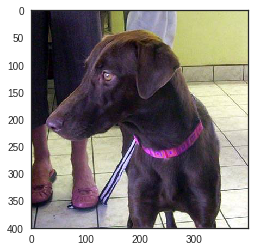
\includegraphics{CNTK-Transfer-Cats-Dogs_files/CNTK-Transfer-Cats-Dogs_33_1.png}
\caption{png}
\end{figure}

\begin{Shaded}
\begin{Highlighting}[]
\NormalTok{img }\OperatorTok{=}\NormalTok{ mpimg.imread(train_cats[random.randint(}\DecValTok{0}\NormalTok{, }\BuiltInTok{len}\NormalTok{(train_cats))])}
\NormalTok{plt.imshow(img)}
\end{Highlighting}
\end{Shaded}

\begin{verbatim}
<matplotlib.image.AxesImage at 0x7faf306df4a8>
\end{verbatim}

\begin{figure}
\centering
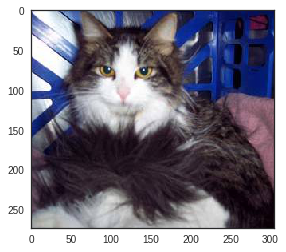
\includegraphics{CNTK-Transfer-Cats-Dogs_files/CNTK-Transfer-Cats-Dogs_34_1.png}
\caption{png}
\end{figure}

\begin{Shaded}
\begin{Highlighting}[]
\KeywordTok{def}\NormalTok{ show_pics(paths: }\BuiltInTok{list}\NormalTok{):}
    
\NormalTok{    f, ax }\OperatorTok{=}\NormalTok{ plt.subplots(}\DecValTok{1}\NormalTok{, }\BuiltInTok{len}\NormalTok{(paths))}
    
    \ControlFlowTok{for}\NormalTok{ i, path }\KeywordTok{in} \BuiltInTok{enumerate}\NormalTok{(paths):}
\NormalTok{        ax[i].imshow(Image.}\BuiltInTok{open}\NormalTok{(path))}
\NormalTok{        ax[i].set_title(os.path.basename(path))}
\NormalTok{        ax[i].axis(}\StringTok{'off'}\NormalTok{)}
\end{Highlighting}
\end{Shaded}

\begin{Shaded}
\begin{Highlighting}[]
\NormalTok{dog_sample }\OperatorTok{=}\NormalTok{ train_dogs[}\DecValTok{0}\NormalTok{:}\DecValTok{3}\NormalTok{]}
\NormalTok{cat_sample }\OperatorTok{=}\NormalTok{ train_cats[}\DecValTok{0}\NormalTok{:}\DecValTok{3}\NormalTok{]}
\end{Highlighting}
\end{Shaded}

\begin{Shaded}
\begin{Highlighting}[]
\NormalTok{show_pics(dog_sample)}
\end{Highlighting}
\end{Shaded}

\begin{figure}
\centering
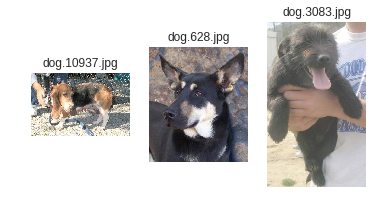
\includegraphics{CNTK-Transfer-Cats-Dogs_files/CNTK-Transfer-Cats-Dogs_37_0.png}
\caption{png}
\end{figure}

\begin{Shaded}
\begin{Highlighting}[]
\NormalTok{show_pics(cat_sample)}
\end{Highlighting}
\end{Shaded}

\begin{figure}
\centering
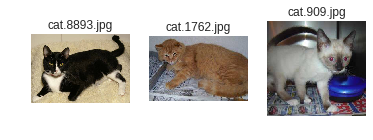
\includegraphics{CNTK-Transfer-Cats-Dogs_files/CNTK-Transfer-Cats-Dogs_38_0.png}
\caption{png}
\end{figure}

\section{Training the Transfer Model}\label{training-the-transfer-model}

Okay, back to our model. Let's take a look at those node labels again.
The last labels are the cross-entropy term, errors, and top-5 errors.
These are needed to define our full computational graph and for training
through backpropagation. The last actual label is \texttt{z}, which maps
to our class labels (1000 in this case, for the number of classes in
\href{http://www.image-net.org/}{ImageNet}). The last activation layer
\emph{prior} to the dense mapping to ImageNet classes is \texttt{z.x}.

\begin{Shaded}
\begin{Highlighting}[]
\NormalTok{C.logging.get_node_outputs(C.load_model(base_model[}\StringTok{'model_file'}\NormalTok{]))}
\end{Highlighting}
\end{Shaded}

\begin{verbatim}
[Output('ce', [], []),
 Output('errs', [], []),
 Output('top5Errs', [], []),
 Output('z', [#, ], [1000]),
 Output('ce', [], []),
 Output('z', [#, ], [1000]),
 Output('z.PlusArgs[0]', [#, ], [1000]),
 Output('z.x', [#, ], [512 x 1 x 1]),
 Output('z.x.x.r', [#, ], [512 x 7 x 7]),
 Output('z.x.x.p', [#, ], [512 x 7 x 7]),
 Output('z.x.x.b', [#, ], [512 x 7 x 7]),
 Output('z.x.x.b.x.c', [#, ], [512 x 7 x 7]),
 Output('z.x.x.b.x', [#, ], [512 x 7 x 7]),
 Output('z.x.x.b.x._', [#, ], [512 x 7 x 7]),
 Output('z.x.x.b.x._.x.c', [#, ], [512 x 7 x 7]),
 Output('z.x.x.x.r', [#, ], [512 x 7 x 7]),
 Output('z.x.x.x.p', [#, ], [512 x 7 x 7]),
 Output('z.x.x.x.b', [#, ], [512 x 7 x 7]),
 Output('z.x.x.x.b.x.c', [#, ], [512 x 7 x 7]),
 Output('z.x.x.x.b.x', [#, ], [512 x 7 x 7]),
 Output('z.x.x.x.b.x._', [#, ], [512 x 7 x 7]),
 Output('z.x.x.x.b.x._.x.c', [#, ], [512 x 7 x 7]),
 Output('_z.x.x.x.r', [#, ], [512 x 7 x 7]),
 Output('_z.x.x.x.p', [#, ], [512 x 7 x 7]),
 Output('_z.x.x.x.b', [#, ], [512 x 7 x 7]),
 Output('_z.x.x.x.b.x.c', [#, ], [512 x 7 x 7]),
 Output('_z.x.x.x.b.x', [#, ], [512 x 7 x 7]),
 Output('_z.x.x.x.b.x._', [#, ], [512 x 7 x 7]),
 Output('_z.x.x.x.b.x._.x.c', [#, ], [512 x 7 x 7]),
 Output('z.x.x.x.x.r', [#, ], [256 x 14 x 14]),
 Output('z.x.x.x.x.p', [#, ], [256 x 14 x 14]),
 Output('z.x.x.x.x.b', [#, ], [256 x 14 x 14]),
 Output('z.x.x.x.x.b.x.c', [#, ], [256 x 14 x 14]),
 Output('z.x.x.x.x.b.x', [#, ], [256 x 14 x 14]),
 Output('z.x.x.x.x.b.x._', [#, ], [256 x 14 x 14]),
 Output('z.x.x.x.x.b.x._.x.c', [#, ], [256 x 14 x 14]),
 Output('z.x.x.x.x.x.r', [#, ], [256 x 14 x 14]),
 Output('z.x.x.x.x.x.p', [#, ], [256 x 14 x 14]),
 Output('z.x.x.x.x.x.b', [#, ], [256 x 14 x 14]),
 Output('z.x.x.x.x.x.b.x.c', [#, ], [256 x 14 x 14]),
 Output('z.x.x.x.x.x.b.x', [#, ], [256 x 14 x 14]),
 Output('z.x.x.x.x.x.b.x._', [#, ], [256 x 14 x 14]),
 Output('z.x.x.x.x.x.b.x._.x.c', [#, ], [256 x 14 x 14]),
 Output('z.x.x.x.x.x.x.r', [#, ], [128 x 28 x 28]),
 Output('z.x.x.x.x.x.x.p', [#, ], [128 x 28 x 28]),
 Output('z.x.x.x.x.x.x.b', [#, ], [128 x 28 x 28]),
 Output('z.x.x.x.x.x.x.b.x.c', [#, ], [128 x 28 x 28]),
 Output('z.x.x.x.x.x.x.b.x', [#, ], [128 x 28 x 28]),
 Output('z.x.x.x.x.x.x.b.x._', [#, ], [128 x 28 x 28]),
 Output('z.x.x.x.x.x.x.b.x._.x.c', [#, ], [128 x 28 x 28]),
 Output('z.x.x.x.x.x.x.x.r', [#, ], [128 x 28 x 28]),
 Output('z.x.x.x.x.x.x.x.p', [#, ], [128 x 28 x 28]),
 Output('z.x.x.x.x.x.x.x.b', [#, ], [128 x 28 x 28]),
 Output('z.x.x.x.x.x.x.x.b.x.c', [#, ], [128 x 28 x 28]),
 Output('z.x.x.x.x.x.x.x.b.x', [#, ], [128 x 28 x 28]),
 Output('z.x.x.x.x.x.x.x.b.x._', [#, ], [128 x 28 x 28]),
 Output('z.x.x.x.x.x.x.x.b.x._.x.c', [#, ], [128 x 28 x 28]),
 Output('z.x.x.x.x.x.x.x.x.r', [#, ], [64 x 56 x 56]),
 Output('z.x.x.x.x.x.x.x.x.p', [#, ], [64 x 56 x 56]),
 Output('z.x.x.x.x.x.x.x.x.b', [#, ], [64 x 56 x 56]),
 Output('z.x.x.x.x.x.x.x.x.b.x.c', [#, ], [64 x 56 x 56]),
 Output('z.x.x.x.x.x.x.x.x.b.x', [#, ], [64 x 56 x 56]),
 Output('z.x.x.x.x.x.x.x.x.b.x._', [#, ], [64 x 56 x 56]),
 Output('z.x.x.x.x.x.x.x.x.b.x._.x.c', [#, ], [64 x 56 x 56]),
 Output('z.x.x.x.x.x.x.x.x.x.r', [#, ], [64 x 56 x 56]),
 Output('z.x.x.x.x.x.x.x.x.x.p', [#, ], [64 x 56 x 56]),
 Output('z.x.x.x.x.x.x.x.x.x.b', [#, ], [64 x 56 x 56]),
 Output('z.x.x.x.x.x.x.x.x.x.b.x.c', [#, ], [64 x 56 x 56]),
 Output('z.x.x.x.x.x.x.x.x.x.b.x', [#, ], [64 x 56 x 56]),
 Output('z.x.x.x.x.x.x.x.x.x.b.x._', [#, ], [64 x 56 x 56]),
 Output('z.x.x.x.x.x.x.x.x.x.b.x._.x.c', [#, ], [64 x 56 x 56]),
 Output('z.x.x.x.x.x.x.x.x.x', [#, ], [64 x 56 x 56]),
 Output('z.x.x.x.x.x.x.x.x.x.x', [#, ], [64 x 112 x 112]),
 Output('z.x.x.x.x.x.x.x.x.x.x._', [#, ], [64 x 112 x 112]),
 Output('z.x.x.x.x.x.x.x.x.x.x._.x.c', [#, ], [64 x 112 x 112]),
 Output('z.x.x.x.x.x.x.x.s', [#, ], [128 x 28 x 28]),
 Output('z.x.x.x.x.x.x.x.s.x.c', [#, ], [128 x 28 x 28]),
 Output('z.x.x.x.x.x.s', [#, ], [256 x 14 x 14]),
 Output('z.x.x.x.x.x.s.x.c', [#, ], [256 x 14 x 14]),
 Output('z.x.x.x.s', [#, ], [512 x 7 x 7]),
 Output('z.x.x.x.s.x.c', [#, ], [512 x 7 x 7]),
 Output('errs', [], []),
 Output('top5Errs', [], [])]
\end{verbatim}

We clone the model so that we can re-use the same trained model multiple
times, trained for different things - it is not strictly necessary if
you are just training it for a single task, but this is why we would not
use \texttt{CloneMethod.share}, we want to learn new parameters. If
\texttt{freeze\_weights} is true, we will freeze weights on all layers
we clone and only learn weights on the final new features layer. This
can often be useful if you are cloning higher up the tree (e.g., cloning
after the first convolutional layer to just get basic image features).

We find the final hidden layer (\texttt{z.x}) using find\_by\_name,
clone it and all of its predecessors, then attach a new \texttt{Dense}
layer for classification.

\begin{Shaded}
\begin{Highlighting}[]
\KeywordTok{def}\NormalTok{ create_model(model_details, num_classes, input_features, }
\NormalTok{                 new_prediction_node_name}\OperatorTok{=}\StringTok{'prediction'}\NormalTok{, freeze}\OperatorTok{=}\VariableTok{False}\NormalTok{):}
\NormalTok{    base_model }\OperatorTok{=}\NormalTok{ C.load_model(model_details[}\StringTok{'model_file'}\NormalTok{])}
\NormalTok{    feature_node }\OperatorTok{=}\NormalTok{ C.logging.find_by_name(base_model, model_details[}\StringTok{'feature_node_name'}\NormalTok{])}
\NormalTok{    last_node }\OperatorTok{=}\NormalTok{ C.logging.find_by_name(base_model, model_details[}\StringTok{'last_hidden_node_name'}\NormalTok{])}

    \CommentTok{# Clone the desired layers with fixed weights}
\NormalTok{    cloned_layers }\OperatorTok{=}\NormalTok{ C.combine([last_node.owner]).clone(}
\NormalTok{        C.CloneMethod.freeze }\ControlFlowTok{if}\NormalTok{ freeze }\ControlFlowTok{else}\NormalTok{ C.CloneMethod.clone,}
\NormalTok{        \{feature_node: C.placeholder(name}\OperatorTok{=}\StringTok{'features'}\NormalTok{)\})}

    \CommentTok{# Add new dense layer for class prediction}
\NormalTok{    feat_norm }\OperatorTok{=}\NormalTok{ input_features}
\NormalTok{    cloned_out }\OperatorTok{=}\NormalTok{ cloned_layers(feat_norm)}
\NormalTok{    z }\OperatorTok{=}\NormalTok{ C.layers.Dense(num_classes, activation}\OperatorTok{=}\VariableTok{None}\NormalTok{, name}\OperatorTok{=}\NormalTok{new_prediction_node_name) (cloned_out)}

    \ControlFlowTok{return}\NormalTok{ z}
\end{Highlighting}
\end{Shaded}

\section{Define Minibatch Source}\label{define-minibatch-source}

Now that we have our model defined, we have to also tell CNTK how to
read in batches to train the model using backprop. Here we'll use the
\href{https://cntk.ai/pythondocs/cntk.io.html\#cntk.io.ImageDeserializer}{\texttt{ImageDeserializer}}
class, designed specifically for the data we have here.

\begin{Shaded}
\begin{Highlighting}[]
\KeywordTok{def}\NormalTok{ create_mb_source(map_file, image_dims, num_classes, randomize}\OperatorTok{=}\VariableTok{True}\NormalTok{):}
\NormalTok{    transforms }\OperatorTok{=}\NormalTok{ [xforms.scale(width}\OperatorTok{=}\NormalTok{image_dims[}\DecValTok{2}\NormalTok{], height}\OperatorTok{=}\NormalTok{image_dims[}\DecValTok{1}\NormalTok{], }
\NormalTok{                               channels}\OperatorTok{=}\NormalTok{image_dims[}\DecValTok{0}\NormalTok{], interpolations}\OperatorTok{=}\StringTok{'linear'}\NormalTok{)]}
    \ControlFlowTok{return}\NormalTok{ C.io.MinibatchSource(C.io.ImageDeserializer(map_file, C.io.StreamDefs(}
\NormalTok{            features}\OperatorTok{=}\NormalTok{C.io.StreamDef(field}\OperatorTok{=}\StringTok{'image'}\NormalTok{, transforms}\OperatorTok{=}\NormalTok{transforms),}
\NormalTok{            labels}\OperatorTok{=}\NormalTok{C.io.StreamDef(field}\OperatorTok{=}\StringTok{'label'}\NormalTok{, shape}\OperatorTok{=}\NormalTok{num_classes))),}
\NormalTok{            randomize}\OperatorTok{=}\NormalTok{randomize)}
\end{Highlighting}
\end{Shaded}

\section{Training}\label{training}

Now our setup is nearly complete. We have our network architecture
defined, and our minibatch reader setup. The last step is defining the
loss function for our optimization algorithm (in this case
\texttt{binary\_cross\_entropy}, or \texttt{cross\_entropy\_softmax} if
we had more than two classes). We'll use a specific learning routine
with a momentum schedule, and simple \(\ell_2\) regularization penalty
on our model's weight terms.

\begin{Shaded}
\begin{Highlighting}[]
\KeywordTok{def}\NormalTok{ train_model(model_details, num_classes, train_map_file,}
\NormalTok{                learning_params, max_images}\OperatorTok{=-}\DecValTok{1}\NormalTok{):}
\NormalTok{    num_epochs }\OperatorTok{=}\NormalTok{ learning_params[}\StringTok{'max_epochs'}\NormalTok{]}
\NormalTok{    epoch_size }\OperatorTok{=} \BuiltInTok{sum}\NormalTok{(}\DecValTok{1} \ControlFlowTok{for}\NormalTok{ line }\KeywordTok{in} \BuiltInTok{open}\NormalTok{(train_map_file))}
    \ControlFlowTok{if}\NormalTok{ max_images }\OperatorTok{>} \DecValTok{0}\NormalTok{:}
\NormalTok{        epoch_size }\OperatorTok{=} \BuiltInTok{min}\NormalTok{(epoch_size, max_images)}
\NormalTok{    minibatch_size }\OperatorTok{=}\NormalTok{ learning_params[}\StringTok{'mb_size'}\NormalTok{]}
    
    \CommentTok{# Create the minibatch source and input variables}
\NormalTok{    minibatch_source }\OperatorTok{=}\NormalTok{ create_mb_source(train_map_file, model_details[}\StringTok{'image_dims'}\NormalTok{], num_classes)}
\NormalTok{    image_input }\OperatorTok{=}\NormalTok{ C.input_variable(model_details[}\StringTok{'image_dims'}\NormalTok{])}
\NormalTok{    label_input }\OperatorTok{=}\NormalTok{ C.input_variable(num_classes)}

    \CommentTok{# Define mapping from reader streams to network inputs}
\NormalTok{    input_map }\OperatorTok{=}\NormalTok{ \{}
\NormalTok{        image_input: minibatch_source[}\StringTok{'features'}\NormalTok{],}
\NormalTok{        label_input: minibatch_source[}\StringTok{'labels'}\NormalTok{]}
\NormalTok{    \}}

    \CommentTok{# Instantiate the transfer learning model and loss function}
\NormalTok{    tl_model }\OperatorTok{=}\NormalTok{ create_model(model_details, num_classes, image_input, freeze}\OperatorTok{=}\NormalTok{learning_params[}\StringTok{'freeze_weights'}\NormalTok{])}
\NormalTok{    ce }\OperatorTok{=}\NormalTok{ C.binary_cross_entropy(tl_model, label_input)}
\NormalTok{    pe }\OperatorTok{=}\NormalTok{ C.classification_error(tl_model, label_input)}

    \CommentTok{# Instantiate the trainer object}
\NormalTok{    lr_schedule }\OperatorTok{=}\NormalTok{ C.learning_rate_schedule(learning_params[}\StringTok{'lr_per_mb'}\NormalTok{], unit}\OperatorTok{=}\NormalTok{C.UnitType.minibatch)}
\NormalTok{    mm_schedule }\OperatorTok{=}\NormalTok{ C.momentum_schedule(learning_params[}\StringTok{'momentum_per_mb'}\NormalTok{])}
\NormalTok{    learner }\OperatorTok{=}\NormalTok{ C.momentum_sgd(tl_model.parameters, lr_schedule, mm_schedule, }
\NormalTok{                           l2_regularization_weight}\OperatorTok{=}\NormalTok{learning_params[}\StringTok{'l2_reg_weight'}\NormalTok{])}
\NormalTok{    trainer }\OperatorTok{=}\NormalTok{ C.Trainer(tl_model, (ce, pe), learner)}

    \CommentTok{# Get minibatches of images and perform model training}
    \BuiltInTok{print}\NormalTok{(}\StringTok{"Training transfer learning model for }\SpecialCharTok{\{0\}}\StringTok{ epochs (epoch_size = }\SpecialCharTok{\{1\}}\StringTok{)."}\NormalTok{.}\BuiltInTok{format}\NormalTok{(num_epochs, epoch_size))}
\NormalTok{    C.logging.log_number_of_parameters(tl_model)}
\NormalTok{    progress_printer }\OperatorTok{=}\NormalTok{ C.logging.ProgressPrinter(tag}\OperatorTok{=}\StringTok{'Training'}\NormalTok{, num_epochs}\OperatorTok{=}\NormalTok{num_epochs)}
    \ControlFlowTok{for}\NormalTok{ epoch }\KeywordTok{in} \BuiltInTok{range}\NormalTok{(num_epochs):       }\CommentTok{# loop over epochs}
\NormalTok{        sample_count }\OperatorTok{=} \DecValTok{0}
        \ControlFlowTok{while}\NormalTok{ sample_count }\OperatorTok{<}\NormalTok{ epoch_size:  }\CommentTok{# loop over minibatches in the epoch}
\NormalTok{            data }\OperatorTok{=}\NormalTok{ minibatch_source.next_minibatch(}\BuiltInTok{min}\NormalTok{(minibatch_size, epoch_size }\OperatorTok{-}\NormalTok{ sample_count), input_map}\OperatorTok{=}\NormalTok{input_map)}
\NormalTok{            trainer.train_minibatch(data)                                    }\CommentTok{# update model with it}
\NormalTok{            sample_count }\OperatorTok{+=}\NormalTok{ trainer.previous_minibatch_sample_count          }\CommentTok{# count samples processed so far}
\NormalTok{            progress_printer.update_with_trainer(trainer, with_metric}\OperatorTok{=}\VariableTok{True}\NormalTok{)  }\CommentTok{# log progress}
            \ControlFlowTok{if}\NormalTok{ sample_count }\OperatorTok{%}\NormalTok{ (}\DecValTok{100} \OperatorTok{*}\NormalTok{ minibatch_size) }\OperatorTok{==} \DecValTok{0}\NormalTok{:}
                \BuiltInTok{print}\NormalTok{ (}\StringTok{"Processed }\SpecialCharTok{\{0\}}\StringTok{ samples"}\NormalTok{.}\BuiltInTok{format}\NormalTok{(sample_count))}

\NormalTok{        progress_printer.epoch_summary(with_metric}\OperatorTok{=}\VariableTok{True}\NormalTok{)}

    \ControlFlowTok{return}\NormalTok{ tl_model}
\end{Highlighting}
\end{Shaded}

\begin{Shaded}
\begin{Highlighting}[]
\NormalTok{force_retraining }\OperatorTok{=} \VariableTok{True}

\NormalTok{max_training_epochs }\OperatorTok{=} \DecValTok{10}

\NormalTok{learning_params }\OperatorTok{=}\NormalTok{ \{}
    \StringTok{'max_epochs'}\NormalTok{: max_training_epochs,}
    \StringTok{'mb_size'}\NormalTok{: }\DecValTok{50}\NormalTok{,}
    \StringTok{'lr_per_mb'}\NormalTok{: [}\FloatTok{0.2}\NormalTok{]}\OperatorTok{*}\DecValTok{10} \OperatorTok{+}\NormalTok{ [}\FloatTok{0.1}\NormalTok{],}
    \StringTok{'momentum_per_mb'}\NormalTok{: }\FloatTok{0.9}\NormalTok{,}
    \StringTok{'l2_reg_weight'}\NormalTok{: }\FloatTok{0.0005}\NormalTok{,}
    \StringTok{'freeze_weights'}\NormalTok{: }\VariableTok{True}
\NormalTok{\}}
\end{Highlighting}
\end{Shaded}

\begin{Shaded}
\begin{Highlighting}[]
\NormalTok{kitty_doggo_model }\OperatorTok{=}\NormalTok{ \{}
    \StringTok{'model_file'}\NormalTok{: os.path.join(}\StringTok{'DogsCats.model'}\NormalTok{),}
    \StringTok{'results_file'}\NormalTok{: os.path.join(}\StringTok{'predictions.txt'}\NormalTok{),}
    \StringTok{'num_classes'}\NormalTok{: }\DecValTok{2}
\NormalTok{\}}
\end{Highlighting}
\end{Shaded}

\begin{Shaded}
\begin{Highlighting}[]
\ControlFlowTok{if}\NormalTok{ os.path.isfile(kitty_doggo_model[}\StringTok{'model_file'}\NormalTok{]):}
    \BuiltInTok{print}\NormalTok{(}\StringTok{"Reload stored model from }\SpecialCharTok{%s}\StringTok{"}\NormalTok{, kitty_doggo_model[}\StringTok{'model_file'}\NormalTok{])}
\NormalTok{    trained_model }\OperatorTok{=}\NormalTok{ C.load_model(kitty_doggo_model[}\StringTok{'model_file'}\NormalTok{])}
\ControlFlowTok{else}\NormalTok{:}
    \BuiltInTok{print}\NormalTok{(}\StringTok{"Retraining model and saving to }\SpecialCharTok{%s}\StringTok{"}\NormalTok{, kitty_doggo_model[}\StringTok{'model_file'}\NormalTok{])}
\NormalTok{    trained_model }\OperatorTok{=}\NormalTok{ train_model(base_model,}
\NormalTok{                              kitty_doggo_model[}\StringTok{'num_classes'}\NormalTok{], }
\NormalTok{                              base_model[}\StringTok{'training_map'}\NormalTok{],}
\NormalTok{                              learning_params)}
\end{Highlighting}
\end{Shaded}

\begin{verbatim}
Reload stored model from %s DogsCats.model
\end{verbatim}

\begin{Shaded}
\begin{Highlighting}[]
\NormalTok{trained_model.save(kitty_doggo_model[}\StringTok{'model_file'}\NormalTok{])}
\BuiltInTok{print}\NormalTok{(}\StringTok{"Stored trained model at }\SpecialCharTok\NormalTok{ kitty_doggo_model[}\StringTok{'model_file'}\NormalTok{])}
\end{Highlighting}
\end{Shaded}

\begin{verbatim}
Stored trained model at DogsCats.model
\end{verbatim}

\begin{Shaded}
\begin{Highlighting}[]
\CommentTok{# Evaluates a single image using the re-trained model}
\KeywordTok{def}\NormalTok{ eval_single_image(loaded_model, image_path, image_dims):}
    \CommentTok{# load and format image (resize, RGB -> BGR, CHW -> HWC)}
    \ControlFlowTok{try}\NormalTok{:}
\NormalTok{        img }\OperatorTok{=}\NormalTok{ Image.}\BuiltInTok{open}\NormalTok{(image_path)}

        \ControlFlowTok{if}\NormalTok{ image_path.endswith(}\StringTok{"png"}\NormalTok{):}
\NormalTok{            temp }\OperatorTok{=}\NormalTok{ Image.new(}\StringTok{"RGB"}\NormalTok{, img.size, (}\DecValTok{255}\NormalTok{, }\DecValTok{255}\NormalTok{, }\DecValTok{255}\NormalTok{))}
\NormalTok{            temp.paste(img, img)}
\NormalTok{            img }\OperatorTok{=}\NormalTok{ temp}
\NormalTok{        resized }\OperatorTok{=}\NormalTok{ img.resize((image_dims[}\DecValTok{2}\NormalTok{], image_dims[}\DecValTok{1}\NormalTok{]), Image.ANTIALIAS)}
\NormalTok{        bgr_image }\OperatorTok{=}\NormalTok{ np.asarray(resized, dtype}\OperatorTok{=}\NormalTok{np.float32)[..., [}\DecValTok{2}\NormalTok{, }\DecValTok{1}\NormalTok{, }\DecValTok{0}\NormalTok{]]}
\NormalTok{        hwc_format }\OperatorTok{=}\NormalTok{ np.ascontiguousarray(np.rollaxis(bgr_image, }\DecValTok{2}\NormalTok{))}

        \CommentTok{# compute model output}
\NormalTok{        arguments }\OperatorTok{=}\NormalTok{ \{loaded_model.arguments[}\DecValTok{0}\NormalTok{]: [hwc_format]\}}
\NormalTok{        output }\OperatorTok{=}\NormalTok{ loaded_model.}\BuiltInTok{eval}\NormalTok{(arguments)}

        \CommentTok{# return softmax probabilities}
\NormalTok{        sm }\OperatorTok{=}\NormalTok{ C.softmax(output[}\DecValTok{0}\NormalTok{])}
        \ControlFlowTok{return}\NormalTok{ sm.}\BuiltInTok{eval}\NormalTok{()}
    \ControlFlowTok{except} \PreprocessorTok{FileNotFoundError}\NormalTok{:}
        \BuiltInTok{print}\NormalTok{(}\StringTok{"Could not open (skipping file): "}\NormalTok{, image_path)}
        \ControlFlowTok{return}\NormalTok{ [}\StringTok{'None'}\NormalTok{]}
\end{Highlighting}
\end{Shaded}

\begin{Shaded}
\begin{Highlighting}[]
\NormalTok{isFast }\OperatorTok{=} \VariableTok{False} \CommentTok{# set to true if you want to evaluate fewer images}
\end{Highlighting}
\end{Shaded}

\begin{Shaded}
\begin{Highlighting}[]
\CommentTok{# Evaluates an image set using the provided model}
\KeywordTok{def}\NormalTok{ eval_test_images(loaded_model, output_file, test_map_file, }
\NormalTok{                     image_dims, max_images}\OperatorTok{=-}\DecValTok{1}\NormalTok{, column_offset}\OperatorTok{=}\DecValTok{0}\NormalTok{):}
\NormalTok{    num_images }\OperatorTok{=} \BuiltInTok{sum}\NormalTok{(}\DecValTok{1} \ControlFlowTok{for}\NormalTok{ line }\KeywordTok{in} \BuiltInTok{open}\NormalTok{(test_map_file))}
    \ControlFlowTok{if}\NormalTok{ max_images }\OperatorTok{>} \DecValTok{0}\NormalTok{:}
\NormalTok{        num_images }\OperatorTok{=} \BuiltInTok{min}\NormalTok{(num_images, max_images)}
    \ControlFlowTok{if}\NormalTok{ isFast:}
\NormalTok{        num_images }\OperatorTok{=} \BuiltInTok{min}\NormalTok{(num_images, }\DecValTok{300}\NormalTok{) }

    \BuiltInTok{print}\NormalTok{(}\StringTok{"Evaluating model output node '}\SpecialCharTok{\{0\}}\StringTok{' for }\SpecialCharTok{\{1\}}\StringTok{ images."}\NormalTok{.}\BuiltInTok{format}\NormalTok{(}\StringTok{'prediction'}\NormalTok{, num_images))}

\NormalTok{    pred_count }\OperatorTok{=} \DecValTok{0}
\NormalTok{    correct_count }\OperatorTok{=} \DecValTok{0}
\NormalTok{    np.seterr(over}\OperatorTok{=}\StringTok{'raise'}\NormalTok{)}
    \ControlFlowTok{with} \BuiltInTok{open}\NormalTok{(output_file, }\StringTok{'wb'}\NormalTok{) }\ImportTok{as}\NormalTok{ results_file:}
        \ControlFlowTok{with} \BuiltInTok{open}\NormalTok{(test_map_file, }\StringTok{"r"}\NormalTok{) }\ImportTok{as}\NormalTok{ input_file:}
            \ControlFlowTok{for}\NormalTok{ line }\KeywordTok{in}\NormalTok{ input_file:}
\NormalTok{                tokens }\OperatorTok{=}\NormalTok{ line.rstrip().split(}\StringTok{'}\CharTok{\textbackslash{}t}\StringTok{'}\NormalTok{)}
\NormalTok{                img_file }\OperatorTok{=}\NormalTok{ tokens[}\DecValTok{0} \OperatorTok{+}\NormalTok{ column_offset]}
\NormalTok{                probs }\OperatorTok{=}\NormalTok{ eval_single_image(loaded_model, img_file, image_dims)}

                \ControlFlowTok{if}\NormalTok{ probs[}\DecValTok{0}\NormalTok{]}\OperatorTok{==}\StringTok{'None'}\NormalTok{:}
                    \BuiltInTok{print}\NormalTok{(}\StringTok{"Eval not possible: "}\NormalTok{, img_file)}
                    \ControlFlowTok{continue}

\NormalTok{                pred_count }\OperatorTok{+=} \DecValTok{1}
\NormalTok{                true_label }\OperatorTok{=} \BuiltInTok{int}\NormalTok{(tokens[}\DecValTok{1} \OperatorTok{+}\NormalTok{ column_offset])}
\NormalTok{                predicted_label }\OperatorTok{=}\NormalTok{ np.argmax(probs)}
                \ControlFlowTok{if}\NormalTok{ predicted_label }\OperatorTok{==}\NormalTok{ true_label:}
\NormalTok{                    correct_count }\OperatorTok{+=} \DecValTok{1}

\NormalTok{                np.savetxt(results_file, probs[np.newaxis], fmt}\OperatorTok{=}\StringTok{"}\SpecialCharTok \DecValTok{100} \OperatorTok{==} \DecValTok{0}\NormalTok{:}
                    \BuiltInTok{print}\NormalTok{(}\StringTok{"Processed }\SpecialCharTok{\{0\}}\StringTok{ samples (}\SpecialCharTok{\{1:.2%\}}\StringTok{ correct)"}\NormalTok{.}\BuiltInTok{format}\NormalTok{(pred_count,}
\NormalTok{                                                                           (}\BuiltInTok{float}\NormalTok{(correct_count) }\OperatorTok{/}\NormalTok{ pred_count)))}
                \ControlFlowTok{if}\NormalTok{ pred_count }\OperatorTok{>=}\NormalTok{ num_images:}
                    \ControlFlowTok{break}
    \BuiltInTok{print}\NormalTok{ (}\StringTok{"}\SpecialCharTok{\{0\}}\StringTok{ of }\SpecialCharTok{\{1\}}\StringTok{ prediction were correct"}\NormalTok{.}\BuiltInTok{format}\NormalTok{(correct_count, pred_count))}
    \ControlFlowTok{return}\NormalTok{ correct_count, pred_count, (}\BuiltInTok{float}\NormalTok{(correct_count) }\OperatorTok{/}\NormalTok{ pred_count)}
\end{Highlighting}
\end{Shaded}

\begin{Shaded}
\begin{Highlighting}[]
\ExtensionTok{%%bash}
\FunctionTok{mkdir}\NormalTok{ val/cats}
\FunctionTok{mkdir}\NormalTok{ val/dogs}
\FunctionTok{mv}\NormalTok{ val/cat.*.jpg ./val/cats/}
\FunctionTok{mv}\NormalTok{ val/dog.*.jpg ./val/dogs}
\end{Highlighting}
\end{Shaded}

\begin{Shaded}
\begin{Highlighting}[]
\NormalTok{class_mapping }\OperatorTok{=}\NormalTok{ create_class_mapping_from_folder(os.path.abspath(path}\OperatorTok{=}\StringTok{"val/"}\NormalTok{))}
\NormalTok{testing_map }\OperatorTok{=}\NormalTok{ create_map_file_from_folder(}\StringTok{"val/"}\NormalTok{, class_mapping)}
\end{Highlighting}
\end{Shaded}

\begin{Shaded}
\begin{Highlighting}[]
\NormalTok{kitty_doggo_model}
\end{Highlighting}
\end{Shaded}

\begin{verbatim}
{'model_file': 'DogsCats.model',
 'num_classes': 2,
 'results_file': 'predictions.txt'}
\end{verbatim}

\begin{Shaded}
\begin{Highlighting}[]
\NormalTok{predict_correct, predict_total, predict_accuracy }\OperatorTok{=} \OperatorTok{\textbackslash{}}
\NormalTok{   eval_test_images(trained_model, kitty_doggo_model[}\StringTok{'results_file'}\NormalTok{], }
\NormalTok{                    testing_map, base_model[}\StringTok{'image_dims'}\NormalTok{])}
\BuiltInTok{print}\NormalTok{(}\StringTok{"Done. Wrote output to }\SpecialCharTok\NormalTok{ kitty_doggo_model[}\StringTok{'results_file'}\NormalTok{])}
\end{Highlighting}
\end{Shaded}

\begin{verbatim}
Evaluating model output node 'prediction' for 5000 images.
Processed 100 samples (97.00% correct)
Processed 200 samples (97.50% correct)
Processed 300 samples (98.33% correct)
Processed 400 samples (98.25% correct)
Processed 500 samples (98.20% correct)
Processed 600 samples (98.50% correct)
Processed 700 samples (98.57% correct)
Processed 800 samples (98.62% correct)
Processed 900 samples (98.22% correct)
Processed 1000 samples (98.40% correct)
Processed 1100 samples (98.27% correct)
Processed 1200 samples (98.00% correct)
Processed 1300 samples (98.08% correct)
Processed 1400 samples (98.07% correct)
Processed 1500 samples (98.07% correct)
Processed 1600 samples (98.00% correct)
Processed 1700 samples (98.06% correct)
Processed 1800 samples (98.06% correct)
Processed 1900 samples (98.05% correct)
Processed 2000 samples (97.95% correct)
Processed 2100 samples (97.90% correct)
Processed 2200 samples (97.86% correct)
Processed 2300 samples (97.91% correct)
Processed 2400 samples (97.83% correct)
Processed 2500 samples (97.84% correct)
Processed 2600 samples (97.77% correct)
Processed 2700 samples (97.81% correct)
Processed 2800 samples (97.86% correct)
Processed 2900 samples (97.90% correct)
Processed 3000 samples (97.90% correct)
Processed 3100 samples (97.87% correct)
Processed 3200 samples (97.88% correct)
Processed 3300 samples (97.91% correct)
Processed 3400 samples (97.94% correct)
Processed 3500 samples (98.00% correct)
Processed 3600 samples (98.00% correct)
Processed 3700 samples (97.97% correct)
Processed 3800 samples (98.00% correct)
Processed 3900 samples (97.97% correct)
Processed 4000 samples (97.95% correct)
Processed 4100 samples (97.93% correct)
Processed 4200 samples (97.95% correct)
Processed 4300 samples (97.98% correct)
Processed 4400 samples (98.00% correct)
Processed 4500 samples (98.02% correct)
Processed 4600 samples (98.00% correct)
Processed 4700 samples (98.02% correct)
Processed 4800 samples (98.04% correct)
Processed 4900 samples (98.02% correct)
Processed 5000 samples (98.06% correct)
4903 of 5000 prediction were correct
Done. Wrote output to predictions.txt
\end{verbatim}

\begin{Shaded}
\begin{Highlighting}[]
\CommentTok{# evaluate test images}
\ControlFlowTok{with} \BuiltInTok{open}\NormalTok{(testing_map, }\StringTok{'r'}\NormalTok{) }\ImportTok{as}\NormalTok{ input_file:}
\NormalTok{    head }\OperatorTok{=} \BuiltInTok{list}\NormalTok{(itertools.islice(input_file, }\DecValTok{15}\NormalTok{))}
    \ControlFlowTok{for}\NormalTok{ line }\KeywordTok{in}\NormalTok{ head:}
\NormalTok{        tokens }\OperatorTok{=}\NormalTok{ line.rstrip().split(}\StringTok{'}\CharTok{\textbackslash{}t}\StringTok{'}\NormalTok{)}
\NormalTok{        img_file }\OperatorTok{=}\NormalTok{ tokens[}\DecValTok{0}\NormalTok{]}
\NormalTok{        true_label }\OperatorTok{=} \BuiltInTok{int}\NormalTok{(tokens[}\DecValTok{1}\NormalTok{])}
\NormalTok{        probs }\OperatorTok{=}\NormalTok{ eval_single_image(trained_model, img_file, base_model[}\StringTok{'image_dims'}\NormalTok{])}

        \ControlFlowTok{if}\NormalTok{ probs[}\DecValTok{0}\NormalTok{]}\OperatorTok{==}\StringTok{'None'}\NormalTok{:}
            \ControlFlowTok{continue}
\NormalTok{        class_probs }\OperatorTok{=}\NormalTok{ np.column_stack((probs, class_mapping)).tolist()}
\NormalTok{        class_probs.sort(key}\OperatorTok{=}\KeywordTok{lambda}\NormalTok{ x: }\BuiltInTok{float}\NormalTok{(x[}\DecValTok{0}\NormalTok{]), reverse}\OperatorTok{=}\VariableTok{True}\NormalTok{)}
\NormalTok{        predictions }\OperatorTok{=} \StringTok{' '}\NormalTok{.join([}\StringTok{'}\SpecialCharTok{%s}\StringTok{:}\SpecialCharTok\NormalTok{ (class_probs[i][}\DecValTok{1}\NormalTok{], }\BuiltInTok{float}\NormalTok{(class_probs[i][}\DecValTok{0}\NormalTok{])) }\OperatorTok{\textbackslash{}}
                                \ControlFlowTok{for}\NormalTok{ i }\KeywordTok{in} \BuiltInTok{range}\NormalTok{(}\DecValTok{0}\NormalTok{, kitty_doggo_model[}\StringTok{'num_classes'}\NormalTok{])])}
\NormalTok{        true_class_name }\OperatorTok{=}\NormalTok{ class_mapping[true_label] }\ControlFlowTok{if}\NormalTok{ true_label }\OperatorTok{>=} \DecValTok{0} \ControlFlowTok{else} \StringTok{'unknown'}
        \BuiltInTok{print}\NormalTok{(}\StringTok{'Class: }\SpecialCharTok{%s}\StringTok{, predictions: }\SpecialCharTok{%s}\StringTok{, image: }\SpecialCharTok\NormalTok{ (true_class_name, predictions, img_file))}
\end{Highlighting}
\end{Shaded}

\begin{verbatim}
Class: cats, predictions: cats:1.000 dogs:0.000, image: val/cats/cat.10001.jpg
Class: cats, predictions: cats:1.000 dogs:0.000, image: val/cats/cat.10003.jpg
Class: cats, predictions: cats:1.000 dogs:0.000, image: val/cats/cat.10005.jpg
Class: cats, predictions: cats:1.000 dogs:0.000, image: val/cats/cat.10006.jpg
Class: cats, predictions: cats:1.000 dogs:0.000, image: val/cats/cat.10010.jpg
Class: cats, predictions: cats:1.000 dogs:0.000, image: val/cats/cat.10016.jpg
Class: cats, predictions: cats:1.000 dogs:0.000, image: val/cats/cat.10017.jpg
Class: cats, predictions: cats:1.000 dogs:0.000, image: val/cats/cat.1002.jpg
Class: cats, predictions: cats:1.000 dogs:0.000, image: val/cats/cat.10032.jpg
Class: cats, predictions: cats:1.000 dogs:0.000, image: val/cats/cat.10033.jpg
Class: cats, predictions: cats:1.000 dogs:0.000, image: val/cats/cat.1004.jpg
Class: cats, predictions: cats:1.000 dogs:0.000, image: val/cats/cat.10047.jpg
Class: cats, predictions: cats:1.000 dogs:0.000, image: val/cats/cat.10054.jpg
Class: cats, predictions: cats:0.995 dogs:0.005, image: val/cats/cat.10058.jpg
Class: cats, predictions: cats:1.000 dogs:0.000, image: val/cats/cat.1006.jpg
\end{verbatim}

\begin{Shaded}
\begin{Highlighting}[]
\KeywordTok{def}\NormalTok{ predictions_df(results}\OperatorTok{=}\NormalTok{kitty_doggo_model[}\StringTok{'results_file'}\NormalTok{], }
\NormalTok{                   key_maps }\OperatorTok{=} \StringTok{"val/map.txt"}\NormalTok{):}
\NormalTok{    preds }\OperatorTok{=}\NormalTok{ pd.read_csv(results, sep}\OperatorTok{=}\StringTok{" "}\NormalTok{, names}\OperatorTok{=}\NormalTok{[}\StringTok{'cat'}\NormalTok{, }\StringTok{'dog'}\NormalTok{])}
\NormalTok{    maps_df }\OperatorTok{=}\NormalTok{ pd.read_csv(key_maps, names}\OperatorTok{=}\NormalTok{[}\StringTok{'path'}\NormalTok{, }\StringTok{'label'}\NormalTok{], sep}\OperatorTok{=}\StringTok{'}\CharTok{\textbackslash{}t}\StringTok{'}\NormalTok{)}
\NormalTok{    preds }\OperatorTok{=}\NormalTok{ pd.concat([preds, maps_df], axis}\OperatorTok{=}\DecValTok{1}\NormalTok{)}
    
    \ControlFlowTok{return}\NormalTok{ preds}
\end{Highlighting}
\end{Shaded}

\begin{Shaded}
\begin{Highlighting}[]
\NormalTok{preds }\OperatorTok{=}\NormalTok{ predictions_df()}
\end{Highlighting}
\end{Shaded}

\begin{Shaded}
\begin{Highlighting}[]
\NormalTok{preds.iloc[}\DecValTok{0}\NormalTok{:}\DecValTok{5}\NormalTok{]}
\end{Highlighting}
\end{Shaded}

\begin{verbatim}
<tr style="text-align: right;">
  <th></th>
  <th>cat</th>
  <th>dog</th>
  <th>path</th>
  <th>label</th>
</tr>
\end{verbatim}

\begin{verbatim}
<tr>
  <th>0</th>
  <td>1.0</td>
  <td>0.0</td>
  <td>val/cats/cat.10001.jpg</td>
  <td>0</td>
</tr>
<tr>
  <th>1</th>
  <td>1.0</td>
  <td>0.0</td>
  <td>val/cats/cat.10003.jpg</td>
  <td>0</td>
</tr>
<tr>
  <th>2</th>
  <td>1.0</td>
  <td>0.0</td>
  <td>val/cats/cat.10005.jpg</td>
  <td>0</td>
</tr>
<tr>
  <th>3</th>
  <td>1.0</td>
  <td>0.0</td>
  <td>val/cats/cat.10006.jpg</td>
  <td>0</td>
</tr>
<tr>
  <th>4</th>
  <td>1.0</td>
  <td>0.0</td>
  <td>val/cats/cat.10010.jpg</td>
  <td>0</td>
</tr>
\end{verbatim}

\begin{Shaded}
\begin{Highlighting}[]
\KeywordTok{def}\NormalTok{ worst_preds(results }\OperatorTok{=}\NormalTok{ preds,}
\NormalTok{               kitties }\OperatorTok{=} \DecValTok{0}\NormalTok{):}
\NormalTok{    results }\OperatorTok{=}\NormalTok{ results[results[}\StringTok{'label'}\NormalTok{] }\OperatorTok{==}\NormalTok{ kitties]}
    \ControlFlowTok{if}\NormalTok{ kitties }\OperatorTok{==} \DecValTok{0}\NormalTok{:}
\NormalTok{        results }\OperatorTok{=}\NormalTok{ results.sort_values(by}\OperatorTok{=}\StringTok{"cat"}\NormalTok{, ascending}\OperatorTok{=}\VariableTok{True}\NormalTok{)}
    \ControlFlowTok{else}\NormalTok{:}
\NormalTok{        results }\OperatorTok{=}\NormalTok{ results.sort_values(by}\OperatorTok{=}\StringTok{"dog"}\NormalTok{, ascending}\OperatorTok{=}\VariableTok{True}\NormalTok{)}
    \ControlFlowTok{return}\NormalTok{ results}
\end{Highlighting}
\end{Shaded}

\begin{Shaded}
\begin{Highlighting}[]
\NormalTok{worst_kitties }\OperatorTok{=}\NormalTok{ worst_preds(kitties }\OperatorTok{=} \DecValTok{0}\NormalTok{)}
\NormalTok{worst_pups }\OperatorTok{=}\NormalTok{ worst_preds(kitties }\OperatorTok{=} \DecValTok{1}\NormalTok{)}
\end{Highlighting}
\end{Shaded}

\begin{Shaded}
\begin{Highlighting}[]
\NormalTok{show_pics(worst_kitties[}\StringTok{'path'}\NormalTok{].iloc[}\DecValTok{0}\NormalTok{:}\DecValTok{5}\NormalTok{])}
\end{Highlighting}
\end{Shaded}

\begin{figure}
\centering
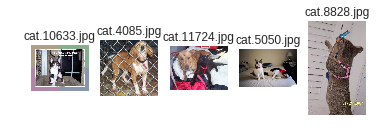
\includegraphics{CNTK-Transfer-Cats-Dogs_files/CNTK-Transfer-Cats-Dogs_64_0.png}
\caption{png}
\end{figure}

\begin{Shaded}
\begin{Highlighting}[]
\NormalTok{show_pics(worst_pups[}\StringTok{'path'}\NormalTok{].iloc[}\DecValTok{0}\NormalTok{:}\DecValTok{5}\NormalTok{])}
\end{Highlighting}
\end{Shaded}

\begin{figure}
\centering
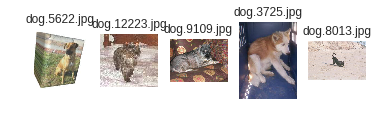
\includegraphics{CNTK-Transfer-Cats-Dogs_files/CNTK-Transfer-Cats-Dogs_65_0.png}
\caption{png}
\end{figure}

\chapter{Fashion MNIST}\label{fashion-mnist}

A MNIST-like dataset for fashion items. See the
\href{https://github.com/zalandoresearch/fashion-mnist}{original
repository} for more information and visualization examples.

\section{Import Core Libraries and Specify Keras
Backend}\label{import-core-libraries-and-specify-keras-backend}

First, we'll import some core libraries and some helper functions. Also
note that we are updating the \texttt{KERAS\_BACKEND} variable to point
to \texttt{CNTK} rather than \texttt{TensorFlow} or \texttt{Theano}.
This is a convenient way of doing this interactively in a single
session. If you'd like to make this your default, modify the
\texttt{\textasciitilde{}/.keras/keras.json} file to always point to
CNTK.

\begin{Shaded}
\begin{Highlighting}[]
\ImportTok{import}\NormalTok{ os}
\NormalTok{os.environ[}\StringTok{'KERAS_BACKEND'}\NormalTok{] }\OperatorTok{=} \StringTok{"cntk"}

\ImportTok{import}\NormalTok{ sys}
\ImportTok{import}\NormalTok{ urllib}

\ImportTok{from}\NormalTok{ keras.layers }\ImportTok{import}\NormalTok{ Dense, Dropout, Flatten}
\ImportTok{from}\NormalTok{ keras.layers }\ImportTok{import}\NormalTok{ Conv2D, MaxPooling2D}
\ImportTok{from}\NormalTok{ keras.layers.normalization }\ImportTok{import}\NormalTok{ BatchNormalization}

\ImportTok{from}\NormalTok{ keras.models }\ImportTok{import}\NormalTok{ Sequential}
\ImportTok{from}\NormalTok{ keras.utils }\ImportTok{import}\NormalTok{ to_categorical}

\ImportTok{from}\NormalTok{ keras.callbacks }\ImportTok{import}\NormalTok{ ModelCheckpoint, TensorBoard}
\ImportTok{from}\NormalTok{ keras }\ImportTok{import}\NormalTok{ optimizers}
\ImportTok{from}\NormalTok{ keras }\ImportTok{import}\NormalTok{ losses}

\ImportTok{from}\NormalTok{ fashion_import }\ImportTok{import}\NormalTok{ load_data}

\ImportTok{import}\NormalTok{ numpy }\ImportTok{as}\NormalTok{ np}
\ImportTok{from}\NormalTok{ PIL }\ImportTok{import}\NormalTok{ Image}
\ImportTok{from}\NormalTok{ io }\ImportTok{import}\NormalTok{ BytesIO}
\end{Highlighting}
\end{Shaded}

\begin{verbatim}
Using CNTK backend
\end{verbatim}

\section{Downloading Fashion Dataset}\label{downloading-fashion-dataset}

The Fashion dataset is not yet preloaded into Keras. We have a simple
helper function called \texttt{load\_data} which will load the data into
memory for us.

\begin{Shaded}
\begin{Highlighting}[]
\NormalTok{(x_train, y_train), (x_test, y_test) }\OperatorTok{=}\NormalTok{ load_data()}
\end{Highlighting}
\end{Shaded}

\begin{verbatim}
Downloading data from http://fashion-mnist.s3-website.eu-central-1.amazonaws.com/train-labels-idx1-ubyte.gz
16384/29515 [===============>..............] - ETA: 0sDownloading data from http://fashion-mnist.s3-website.eu-central-1.amazonaws.com/train-images-idx3-ubyte.gz
23953408/26421880 [==========================>...] - ETA: 0sDownloading data from http://fashion-mnist.s3-website.eu-central-1.amazonaws.com/t10k-labels-idx1-ubyte.gz
8192/5148 [===============================================] - 0s
Downloading data from http://fashion-mnist.s3-website.eu-central-1.amazonaws.com/t10k-images-idx3-ubyte.gz
3260416/4422102 [=====================>........] - ETA: 0s
\end{verbatim}

\section{Scale Data and Visualize}\label{scale-data-and-visualize}

Now that we have our data ingested into memory, let's scale it into unit
range and visualize a few examples.

\begin{Shaded}
\begin{Highlighting}[]
\NormalTok{x_train }\OperatorTok{=}\NormalTok{ x_train.reshape(}\DecValTok{60000}\NormalTok{, }\DecValTok{28}\NormalTok{, }\DecValTok{28}\NormalTok{, }\DecValTok{1}\NormalTok{)}
\NormalTok{x_test }\OperatorTok{=}\NormalTok{ x_test.reshape(}\DecValTok{10000}\NormalTok{, }\DecValTok{28}\NormalTok{, }\DecValTok{28}\NormalTok{, }\DecValTok{1}\NormalTok{)}
\NormalTok{x_train }\OperatorTok{=}\NormalTok{ x_train.astype(}\StringTok{'float32'}\NormalTok{)}
\NormalTok{x_test }\OperatorTok{=}\NormalTok{ x_test.astype(}\StringTok{'float32'}\NormalTok{)}
\NormalTok{x_train }\OperatorTok{/=} \DecValTok{255}
\NormalTok{x_test }\OperatorTok{/=} \DecValTok{255}

\CommentTok{# convert class vectors to binary class matrices}
\NormalTok{y_train }\OperatorTok{=}\NormalTok{ to_categorical(y_train, }\DecValTok{10}\NormalTok{)}
\NormalTok{y_test }\OperatorTok{=}\NormalTok{ to_categorical(y_test, }\DecValTok{10}\NormalTok{)}
\end{Highlighting}
\end{Shaded}

\begin{Shaded}
\begin{Highlighting}[]
\ImportTok{import}\NormalTok{ matplotlib.pyplot }\ImportTok{as}\NormalTok{ plt}
\OperatorTok{%}\NormalTok{matplotlib inline}
\NormalTok{pixels }\OperatorTok{=}\NormalTok{ x_train[}\DecValTok{10}\NormalTok{].reshape((}\DecValTok{28}\NormalTok{, }\DecValTok{28}\NormalTok{))}
\NormalTok{plt.imshow(pixels)}
\NormalTok{plt.show()}
\end{Highlighting}
\end{Shaded}

\begin{figure}
\centering
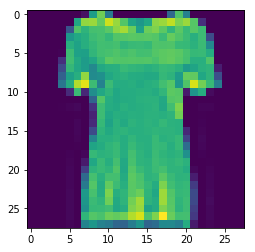
\includegraphics{output_5_0.png}
\caption{png}
\end{figure}

\section{Create Network Architecture and Model
Parameters}\label{create-network-architecture-and-model-parameters}

Keras has a very simple high-level sequential and functional API for
defining network architectures. Here we'll use the sequential API and
compile our model with a common optimization algorithm and loss metrics.

\begin{Shaded}
\begin{Highlighting}[]
\NormalTok{batch_size }\OperatorTok{=} \DecValTok{256}
\NormalTok{num_classes }\OperatorTok{=} \DecValTok{10}
\NormalTok{epochs }\OperatorTok{=} \DecValTok{10}

\NormalTok{img_rows, img_cols }\OperatorTok{=} \DecValTok{28}\NormalTok{, }\DecValTok{28}
\NormalTok{input_shape }\OperatorTok{=}\NormalTok{ (img_rows, img_cols, }\DecValTok{1}\NormalTok{)}

\NormalTok{model }\OperatorTok{=}\NormalTok{ Sequential()}
\NormalTok{model.add(Conv2D(}\DecValTok{32}\NormalTok{, kernel_size}\OperatorTok{=}\NormalTok{(}\DecValTok{3}\NormalTok{, }\DecValTok{3}\NormalTok{),}
\NormalTok{                 activation}\OperatorTok{=}\StringTok{'relu'}\NormalTok{,}
\NormalTok{                 kernel_initializer}\OperatorTok{=}\StringTok{'he_normal'}\NormalTok{,}
\NormalTok{                 input_shape}\OperatorTok{=}\NormalTok{input_shape))}
\NormalTok{model.add(MaxPooling2D((}\DecValTok{2}\NormalTok{, }\DecValTok{2}\NormalTok{)))}
\NormalTok{model.add(Dropout(}\FloatTok{0.25}\NormalTok{))}
\NormalTok{model.add(Conv2D(}\DecValTok{64}\NormalTok{, (}\DecValTok{3}\NormalTok{, }\DecValTok{3}\NormalTok{), activation}\OperatorTok{=}\StringTok{'relu'}\NormalTok{))}
\NormalTok{model.add(MaxPooling2D(pool_size}\OperatorTok{=}\NormalTok{(}\DecValTok{2}\NormalTok{, }\DecValTok{2}\NormalTok{)))}
\NormalTok{model.add(Dropout(}\FloatTok{0.25}\NormalTok{))}
\NormalTok{model.add(Conv2D(}\DecValTok{128}\NormalTok{, (}\DecValTok{3}\NormalTok{, }\DecValTok{3}\NormalTok{), activation}\OperatorTok{=}\StringTok{'relu'}\NormalTok{))}
\NormalTok{model.add(Dropout(}\FloatTok{0.4}\NormalTok{))}
\NormalTok{model.add(Flatten())}
\NormalTok{model.add(Dense(}\DecValTok{128}\NormalTok{, activation}\OperatorTok{=}\StringTok{'relu'}\NormalTok{))}
\NormalTok{model.add(Dropout(}\FloatTok{0.3}\NormalTok{))}
\NormalTok{model.add(Dense(num_classes, activation}\OperatorTok{=}\StringTok{'softmax'}\NormalTok{))}

\NormalTok{model.}\BuiltInTok{compile}\NormalTok{(loss}\OperatorTok{=}\NormalTok{losses.categorical_crossentropy,}
\NormalTok{              optimizer}\OperatorTok{=}\NormalTok{optimizers.Adam(),}
\NormalTok{              metrics}\OperatorTok{=}\NormalTok{[}\StringTok{'accuracy'}\NormalTok{])}

\NormalTok{model.summary()}
\end{Highlighting}
\end{Shaded}

\begin{verbatim}
_________________________________________________________________
Layer (type)                 Output Shape              Param #   
=================================================================
conv2d_1 (Conv2D)            (None, 26, 26, 32)        320       
_________________________________________________________________
max_pooling2d_1 (MaxPooling2 (None, 13, 13, 32)        0         
_________________________________________________________________
dropout_1 (Dropout)          (None, 13, 13, 32)        0         
_________________________________________________________________
conv2d_2 (Conv2D)            (None, 11, 11, 64)        18496     
_________________________________________________________________
max_pooling2d_2 (MaxPooling2 (None, 5, 5, 64)          0         
_________________________________________________________________
dropout_2 (Dropout)          (None, 5, 5, 64)          0         
_________________________________________________________________
conv2d_3 (Conv2D)            (None, 3, 3, 128)         73856     
_________________________________________________________________
dropout_3 (Dropout)          (None, 3, 3, 128)         0         
_________________________________________________________________
flatten_1 (Flatten)          (None, 1152)              0         
_________________________________________________________________
dense_1 (Dense)              (None, 128)               147584    
_________________________________________________________________
dropout_4 (Dropout)          (None, 128)               0         
_________________________________________________________________
dense_2 (Dense)              (None, 10)                1290      
=================================================================
Total params: 241,546
Trainable params: 241,546
Non-trainable params: 0
_________________________________________________________________
\end{verbatim}

\section{Training Our Model}\label{training-our-model}

Training the model, i.e., backpropagating to fit model parameters to
training data, is as simple as using the \texttt{fit} method in Keras.

\begin{Shaded}
\begin{Highlighting}[]
\NormalTok{history }\OperatorTok{=}\NormalTok{ model.fit(x_train, y_train,}
\NormalTok{          batch_size}\OperatorTok{=}\NormalTok{batch_size,}
\NormalTok{          epochs}\OperatorTok{=}\NormalTok{epochs)}
\end{Highlighting}
\end{Shaded}

\begin{verbatim}
Epoch 1/10


/home/mugen/.conda/envs/cntk-py35/lib/python3.5/site-packages/cntk/core.py:361: UserWarning: your data is of type "float64", but your input variable (uid "Input170") expects "<class 'numpy.float32'>". Please convert your data beforehand to speed up training.
  (sample.dtype, var.uid, str(var.dtype)))


60000/60000 [==============================] - 10s - loss: 0.8519 - acc: 0.6817    
Epoch 2/10
60000/60000 [==============================] - 7s - loss: 0.5029 - acc: 0.8138     
Epoch 3/10
60000/60000 [==============================] - 7s - loss: 0.4330 - acc: 0.8406     
Epoch 4/10
60000/60000 [==============================] - 7s - loss: 0.3867 - acc: 0.8575     
Epoch 5/10
60000/60000 [==============================] - 7s - loss: 0.3595 - acc: 0.8675     
Epoch 6/10
60000/60000 [==============================] - 7s - loss: 0.3365 - acc: 0.8777     
Epoch 7/10
60000/60000 [==============================] - 7s - loss: 0.3203 - acc: 0.8822     
Epoch 8/10
60000/60000 [==============================] - 7s - loss: 0.3112 - acc: 0.8868     
Epoch 9/10
60000/60000 [==============================] - 7s - loss: 0.3001 - acc: 0.8896     
Epoch 10/10
60000/60000 [==============================] - 7s - loss: 0.2889 - acc: 0.8936     
\end{verbatim}

\section{Scoring the Model}\label{scoring-the-model}

Just as simple is scoring it on our test set. We can simply pass the
\texttt{x\_test} and \texttt{y\_test} arrays to the \texttt{evaluate}
method and Keras will score the model for us.

\begin{Shaded}
\begin{Highlighting}[]
\NormalTok{test_val }\OperatorTok{=}\NormalTok{ model.evaluate(x_test, y_test)}
\end{Highlighting}
\end{Shaded}

\begin{verbatim}
 1312/10000 [==>...........................] - ETA: 1s

/anaconda/envs/cntk-22/lib/python3.5/site-packages/cntk/core.py:361: UserWarning: your data is of type "float64", but your input variable (uid "Input170") expects "<class 'numpy.float32'>". Please convert your data beforehand to speed up training.
  (sample.dtype, var.uid, str(var.dtype)))


 9856/10000 [============================>.] - ETA: 0s
\end{verbatim}

\begin{Shaded}
\begin{Highlighting}[]
\BuiltInTok{print}\NormalTok{(}\StringTok{"Model's Accuracy on Test Set = "}
      \OperatorTok{+} \StringTok{"}\SpecialCharTok{\{0:.2f\}}\StringTok{%"}\NormalTok{.}\BuiltInTok{format}\NormalTok{(test_val[}\DecValTok{1}\NormalTok{] }\OperatorTok{*} \DecValTok{100}\NormalTok{))}
\end{Highlighting}
\end{Shaded}

\begin{verbatim}
Model's Accuracy on Test Set = 90.14%
\end{verbatim}

\begin{Shaded}
\begin{Highlighting}[]
\ImportTok{import}\NormalTok{ matplotlib.pyplot }\ImportTok{as}\NormalTok{ plt}
\OperatorTok{%}\NormalTok{matplotlib inline}

\NormalTok{accuracy }\OperatorTok{=}\NormalTok{ history.history[}\StringTok{'acc'}\NormalTok{]}
\CommentTok{# val_accuracy = history.history['val_acc']}
\NormalTok{loss }\OperatorTok{=}\NormalTok{ history.history[}\StringTok{'loss'}\NormalTok{]}
\CommentTok{# val_loss = history.history['val_loss']}
\NormalTok{epochs }\OperatorTok{=} \BuiltInTok{range}\NormalTok{(}\BuiltInTok{len}\NormalTok{(accuracy))}
\NormalTok{plt.plot(epochs, accuracy, }\StringTok{'bo'}\NormalTok{, label}\OperatorTok{=}\StringTok{'Training accuracy'}\NormalTok{)}
\NormalTok{plt.title(}\StringTok{'Training accuracy'}\NormalTok{)}
\NormalTok{plt.legend()}
\NormalTok{plt.figure()}
\NormalTok{plt.plot(epochs, loss, }\StringTok{'bo'}\NormalTok{, label}\OperatorTok{=}\StringTok{'Training loss'}\NormalTok{)}
\NormalTok{plt.title(}\StringTok{'Training loss'}\NormalTok{)}
\NormalTok{plt.legend()}
\NormalTok{plt.show()}
\end{Highlighting}
\end{Shaded}

\begin{figure}
\centering
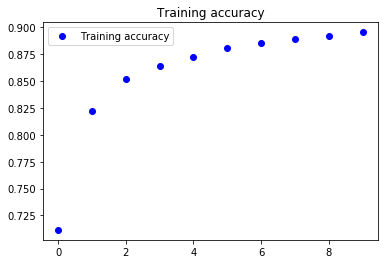
\includegraphics{output_10_0.png}
\caption{png}
\end{figure}

\begin{figure}
\centering
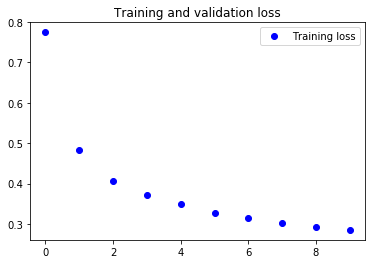
\includegraphics{output_10_1.png}
\caption{png}
\end{figure}

\begin{Shaded}
\begin{Highlighting}[]
\NormalTok{test_im }\OperatorTok{=}\NormalTok{ x_train[}\DecValTok{3}\NormalTok{]}
\NormalTok{plt.imshow(test_im.reshape(}\DecValTok{28}\NormalTok{,}\DecValTok{28}\NormalTok{), cmap}\OperatorTok{=}\StringTok{'gray'}\NormalTok{, interpolation}\OperatorTok{=}\StringTok{'none'}\NormalTok{)}
\NormalTok{plt.show()}
\end{Highlighting}
\end{Shaded}

\begin{figure}
\centering
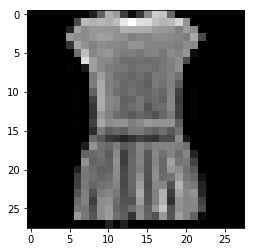
\includegraphics{output_11_0.png}
\caption{png}
\end{figure}

\begin{Shaded}
\begin{Highlighting}[]
\ImportTok{from}\NormalTok{ keras }\ImportTok{import}\NormalTok{ models}
\NormalTok{layer_outputs }\OperatorTok{=}\NormalTok{ [layer.output }\ControlFlowTok{for}\NormalTok{ layer }\KeywordTok{in}\NormalTok{ model.layers[:}\DecValTok{8}\NormalTok{]]}
\NormalTok{activation_model }\OperatorTok{=}\NormalTok{ models.Model(}\BuiltInTok{input}\OperatorTok{=}\NormalTok{model.}\BuiltInTok{input}\NormalTok{, output}\OperatorTok{=}\NormalTok{layer_outputs)}
\NormalTok{activations }\OperatorTok{=}\NormalTok{ activation_model.predict(test_im.reshape(}\DecValTok{1}\NormalTok{,}\DecValTok{28}\NormalTok{,}\DecValTok{28}\NormalTok{,}\DecValTok{1}\NormalTok{))}

\NormalTok{first_layer_activation }\OperatorTok{=}\NormalTok{ activations[}\DecValTok{0}\NormalTok{]}
\NormalTok{plt.matshow(first_layer_activation[}\DecValTok{0}\NormalTok{, :, :, }\DecValTok{4}\NormalTok{], cmap}\OperatorTok{=}\StringTok{'gray'}\NormalTok{)}
\end{Highlighting}
\end{Shaded}

\begin{verbatim}
/anaconda/envs/cntk-22/lib/python3.5/site-packages/ipykernel/__main__.py:3: UserWarning: Update your `Model` call to the Keras 2 API: `Model(outputs=[Composite..., inputs=Input('con...)`
  app.launch_new_instance()





<matplotlib.image.AxesImage at 0x7f08c0f78278>
\end{verbatim}

\begin{figure}
\centering
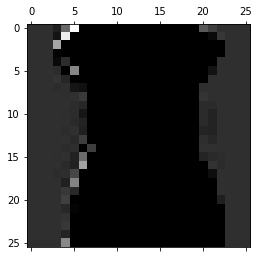
\includegraphics{output_12_2.png}
\caption{png}
\end{figure}

\begin{Shaded}
\begin{Highlighting}[]
\NormalTok{layer_names }\OperatorTok{=}\NormalTok{ []}
\ControlFlowTok{for}\NormalTok{ layer }\KeywordTok{in}\NormalTok{ model.layers[:}\OperatorTok{-}\DecValTok{1}\NormalTok{]:}
    \ControlFlowTok{if} \BuiltInTok{isinstance}\NormalTok{(layer, Conv2D):}
\NormalTok{        layer_names.append(layer.name)}
\NormalTok{images_per_row }\OperatorTok{=} \DecValTok{16}

\ControlFlowTok{for}\NormalTok{ layer_name, layer_activation }\KeywordTok{in} \BuiltInTok{zip}\NormalTok{(layer_names, activations):}
\NormalTok{    n_features }\OperatorTok{=}\NormalTok{ layer_activation.shape[}\OperatorTok{-}\DecValTok{1}\NormalTok{]}
\NormalTok{    size }\OperatorTok{=}\NormalTok{ layer_activation.shape[}\DecValTok{1}\NormalTok{]}
\NormalTok{    n_cols }\OperatorTok{=}\NormalTok{ n_features }\OperatorTok{/}\NormalTok{ images_per_row}
\NormalTok{    n_cols }\OperatorTok{=} \BuiltInTok{int}\NormalTok{(n_cols)}
\NormalTok{    display_grid }\OperatorTok{=}\NormalTok{ np.zeros((size }\OperatorTok{*}\NormalTok{ n_cols, images_per_row }\OperatorTok{*}\NormalTok{ size))}
    \ControlFlowTok{for}\NormalTok{ col }\KeywordTok{in} \BuiltInTok{range}\NormalTok{(n_cols):}
        \ControlFlowTok{for}\NormalTok{ row }\KeywordTok{in} \BuiltInTok{range}\NormalTok{(images_per_row):}
\NormalTok{            channel_image }\OperatorTok{=}\NormalTok{ layer_activation[}\DecValTok{0}\NormalTok{,:, :, col }\OperatorTok{*}\NormalTok{ images_per_row }\OperatorTok{+}\NormalTok{ row]}
\NormalTok{            channel_image }\OperatorTok{-=}\NormalTok{ channel_image.mean()}
\NormalTok{            channel_image }\OperatorTok{/=}\NormalTok{ channel_image.std()}
\NormalTok{            channel_image }\OperatorTok{*=} \DecValTok{64}
\NormalTok{            channel_image }\OperatorTok{+=} \DecValTok{128}
\NormalTok{            channel_image }\OperatorTok{=}\NormalTok{ np.clip(channel_image, }\DecValTok{0}\NormalTok{, }\DecValTok{255}\NormalTok{).astype(}\StringTok{'uint8'}\NormalTok{)}
\NormalTok{            display_grid[col }\OperatorTok{*}\NormalTok{ size : (col }\OperatorTok{+} \DecValTok{1}\NormalTok{) }\OperatorTok{*}\NormalTok{ size,}
\NormalTok{                         row }\OperatorTok{*}\NormalTok{ size : (row }\OperatorTok{+} \DecValTok{1}\NormalTok{) }\OperatorTok{*}\NormalTok{ size] }\OperatorTok{=}\NormalTok{ channel_image}
\NormalTok{    scale }\OperatorTok{=} \DecValTok{1}\NormalTok{. }\OperatorTok{/}\NormalTok{ size}
\NormalTok{    plt.figure(figsize}\OperatorTok{=}\NormalTok{(scale }\OperatorTok{*}\NormalTok{ display_grid.shape[}\DecValTok{1}\NormalTok{],}
\NormalTok{                        scale }\OperatorTok{*}\NormalTok{ display_grid.shape[}\DecValTok{0}\NormalTok{]))}
\NormalTok{    plt.title(layer_name)}
\NormalTok{    plt.grid(}\VariableTok{False}\NormalTok{)}
\NormalTok{    plt.imshow(display_grid, aspect}\OperatorTok{=}\StringTok{'auto'}\NormalTok{, cmap}\OperatorTok{=}\StringTok{'bone'}\NormalTok{)}
\end{Highlighting}
\end{Shaded}

\begin{figure}
\centering
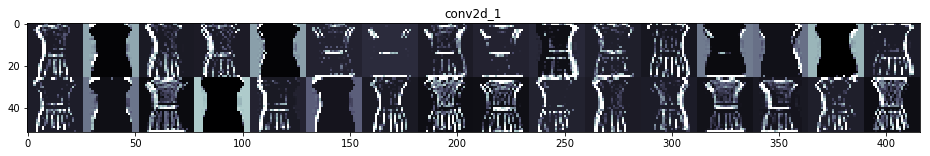
\includegraphics{output_13_0.png}
\caption{png}
\end{figure}

\begin{figure}
\centering
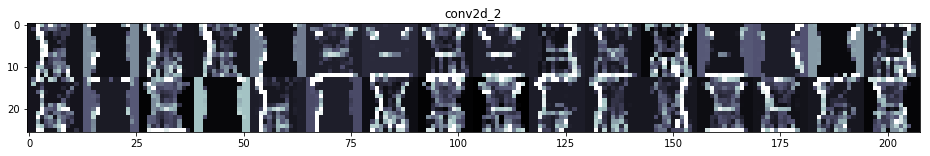
\includegraphics{output_13_1.png}
\caption{png}
\end{figure}

\begin{figure}
\centering
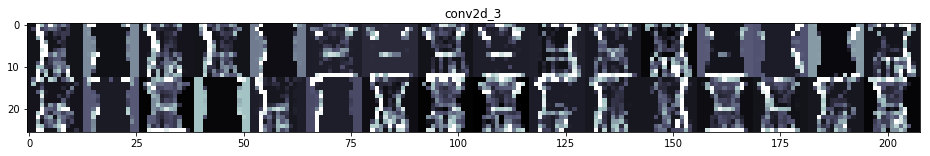
\includegraphics{output_13_2.png}
\caption{png}
\end{figure}

\chapter{Neural Style Transfer}\label{neural-style-transfer}

This tutorial shows how to transfer the style / texture of one image to
another. This allows us to take our ordinary photos and render them in
the style of famous images or paintings.

Apart from creating nice looking pictures, in this tutorial you will
learn how to load a pretrained
\href{https://arxiv.org/abs/1409.1556}{VGG model} into CNTK, how to get
the gradient of a function with respect to an input variable (rather
than a parameter), and how to use the gradient outside of CNTK.

We will follow the approach of
\href{https://arxiv.org/abs/1508.06576}{Gatys et. al.} with some of the
improvements in \href{https://arxiv.org/abs/1605.04603}{Novak and
Nikulin}. While \href{https://arxiv.org/abs/1603.08155}{faster
techniques} exist, these are limited to transfering a particular style.

We begin by importing the necessary packages. In addition to the usual
suspects (\texttt{numpy}, \texttt{scipy}, and \texttt{cntk}) we will
need \texttt{PIL} to work with images, \texttt{requests} to download a
pretrained model and \texttt{h5py} to read in the weights of the
pretrained model.

\begin{Shaded}
\begin{Highlighting}[]
\ImportTok{from}\NormalTok{ __future__ }\ImportTok{import}\NormalTok{ print_function}
\ImportTok{import}\NormalTok{ numpy }\ImportTok{as}\NormalTok{ np}
\ImportTok{from}\NormalTok{ scipy }\ImportTok{import}\NormalTok{ optimize }\ImportTok{as}\NormalTok{ opt}
\ImportTok{import}\NormalTok{ cntk }\ImportTok{as}\NormalTok{ C}
\ImportTok{from}\NormalTok{ PIL }\ImportTok{import}\NormalTok{ Image}
\ImportTok{import}\NormalTok{ requests}
\ImportTok{import}\NormalTok{ h5py}
\ImportTok{import}\NormalTok{ os}
\OperatorTok{%}\NormalTok{matplotlib inline}
\ImportTok{import}\NormalTok{ matplotlib.pyplot }\ImportTok{as}\NormalTok{ plt}
\CommentTok{# Select the right target device when this notebook is being tested:}
\ControlFlowTok{if} \StringTok{'TEST_DEVICE'} \KeywordTok{in}\NormalTok{ os.environ:}
    \ControlFlowTok{if}\NormalTok{ os.environ[}\StringTok{'TEST_DEVICE'}\NormalTok{] }\OperatorTok{==} \StringTok{'cpu'}\NormalTok{:}
\NormalTok{        C.device.try_set_default_device(C.device.cpu())}
    \ControlFlowTok{else}\NormalTok{:}
\NormalTok{        C.device.try_set_default_device(C.device.gpu(}\DecValTok{0}\NormalTok{))}
\end{Highlighting}
\end{Shaded}

The pretrained model is a VGG network which we originally got from
\href{https://gist.github.com/baraldilorenzo/07d7802847aaad0a35d3}{this
page}. We host it in a place which permits easy downloading. Below we
download it if it is not already available locally and load the weights
into numpy arrays.

\begin{Shaded}
\begin{Highlighting}[]
\KeywordTok{def}\NormalTok{ download(url, filename):}
\NormalTok{    response }\OperatorTok{=}\NormalTok{ requests.get(url, stream}\OperatorTok{=}\VariableTok{True}\NormalTok{)}
    \ControlFlowTok{with} \BuiltInTok{open}\NormalTok{(filename, }\StringTok{'wb'}\NormalTok{) }\ImportTok{as}\NormalTok{ handle:}
        \ControlFlowTok{for}\NormalTok{ data }\KeywordTok{in}\NormalTok{ response.iter_content(chunk_size}\OperatorTok{=}\DecValTok{2}\OperatorTok{**}\DecValTok{20}\NormalTok{):}
            \ControlFlowTok{if}\NormalTok{ data: handle.write(data)}


\KeywordTok{def}\NormalTok{ load_vgg(path):}
\NormalTok{    f }\OperatorTok{=}\NormalTok{ h5py.File(path)}
\NormalTok{    layers }\OperatorTok{=}\NormalTok{ []}
    \ControlFlowTok{for}\NormalTok{ k }\KeywordTok{in} \BuiltInTok{range}\NormalTok{(f.attrs[}\StringTok{'nb_layers'}\NormalTok{]):}
\NormalTok{        g }\OperatorTok{=}\NormalTok{ f[}\StringTok{'layer_}\SpecialCharTok{\{\}}\StringTok{'}\NormalTok{.}\BuiltInTok{format}\NormalTok{(k)]}
\NormalTok{        n }\OperatorTok{=}\NormalTok{ g.attrs[}\StringTok{'nb_params'}\NormalTok{]}
\NormalTok{        layers.append([g[}\StringTok{'param_}\SpecialCharTok{\{\}}\StringTok{'}\NormalTok{.}\BuiltInTok{format}\NormalTok{(p)][:] }\ControlFlowTok{for}\NormalTok{ p }\KeywordTok{in} \BuiltInTok{range}\NormalTok{(n)])}
\NormalTok{    f.close()}
    \ControlFlowTok{return}\NormalTok{ layers}

\CommentTok{# Check for an environment variable defined in CNTK's test infrastructure}
\NormalTok{envvar }\OperatorTok{=} \StringTok{'CNTK_EXTERNAL_TESTDATA_SOURCE_DIRECTORY'}
\KeywordTok{def}\NormalTok{ is_test(): }\ControlFlowTok{return}\NormalTok{ envvar }\KeywordTok{in}\NormalTok{ os.environ}

\NormalTok{path }\OperatorTok{=} \StringTok{'vgg16_weights.bin'}
\NormalTok{url }\OperatorTok{=} \StringTok{'https://cntk.ai/jup/models/vgg16_weights.bin'}
\CommentTok{# We check for the model locally}
\ControlFlowTok{if} \KeywordTok{not}\NormalTok{ os.path.exists(path):}
    \CommentTok{# If not there we might be running in CNTK's test infrastructure}
    \ControlFlowTok{if}\NormalTok{ is_test():}
\NormalTok{        path }\OperatorTok{=}\NormalTok{ os.path.join(os.environ[envvar],}\StringTok{'PreTrainedModels'}\NormalTok{,}\StringTok{'Vgg16'}\NormalTok{,}\StringTok{'v0'}\NormalTok{,path)}
    \ControlFlowTok{else}\NormalTok{:}
        \CommentTok{#If neither is true we download the file from the web}
        \BuiltInTok{print}\NormalTok{(}\StringTok{'downloading VGG model (~0.5GB)'}\NormalTok{)}
\NormalTok{        download(url, path)}
\NormalTok{layers }\OperatorTok{=}\NormalTok{ load_vgg(path)}
\BuiltInTok{print}\NormalTok{(}\StringTok{'loaded VGG model'}\NormalTok{)}
\end{Highlighting}
\end{Shaded}

\begin{verbatim}
downloading VGG model (~0.5GB)
loaded VGG model
\end{verbatim}

Next we define the VGG network as a CNTK graph.

\begin{Shaded}
\begin{Highlighting}[]
\CommentTok{# A convolutional layer in the VGG network}
\KeywordTok{def}\NormalTok{ vggblock(x, arrays, layer_map, name):}
\NormalTok{    f }\OperatorTok{=}\NormalTok{ arrays[}\DecValTok{0}\NormalTok{]}
\NormalTok{    b }\OperatorTok{=}\NormalTok{ arrays[}\DecValTok{1}\NormalTok{]}
\NormalTok{    k }\OperatorTok{=}\NormalTok{ C.constant(value}\OperatorTok{=}\NormalTok{f)}
\NormalTok{    t }\OperatorTok{=}\NormalTok{ C.constant(value}\OperatorTok{=}\NormalTok{np.reshape(b, (}\OperatorTok{-}\DecValTok{1}\NormalTok{, }\DecValTok{1}\NormalTok{, }\DecValTok{1}\NormalTok{)))}
\NormalTok{    y }\OperatorTok{=}\NormalTok{ C.relu(C.convolution(k, x, auto_padding}\OperatorTok{=}\NormalTok{[}\VariableTok{False}\NormalTok{, }\VariableTok{True}\NormalTok{, }\VariableTok{True}\NormalTok{]) }\OperatorTok{+}\NormalTok{ t)}
\NormalTok{    layer_map[name] }\OperatorTok{=}\NormalTok{ y}
    \ControlFlowTok{return}\NormalTok{ y}

\CommentTok{# A pooling layer in the VGG network}
\KeywordTok{def}\NormalTok{ vggpool(x):}
    \ControlFlowTok{return}\NormalTok{ C.pooling(x, C.AVG_POOLING, (}\DecValTok{2}\NormalTok{, }\DecValTok{2}\NormalTok{), (}\DecValTok{2}\NormalTok{, }\DecValTok{2}\NormalTok{))}


\CommentTok{# Build the graph for the VGG network (excluding fully connected layers)}
\KeywordTok{def}\NormalTok{ model(x, layers):}
\NormalTok{    model_layers }\OperatorTok{=}\NormalTok{ \{\}}
    \KeywordTok{def}\NormalTok{ convolutional(z): }\ControlFlowTok{return} \BuiltInTok{len}\NormalTok{(z) }\OperatorTok{==} \DecValTok{2} \KeywordTok{and} \BuiltInTok{len}\NormalTok{(z[}\DecValTok{0}\NormalTok{].shape) }\OperatorTok{==} \DecValTok{4}
\NormalTok{    conv }\OperatorTok{=}\NormalTok{ [layer }\ControlFlowTok{for}\NormalTok{ layer }\KeywordTok{in}\NormalTok{ layers }\ControlFlowTok{if}\NormalTok{ convolutional(layer)]}
\NormalTok{    cnt }\OperatorTok{=} \DecValTok{0}
\NormalTok{    num_convs }\OperatorTok{=}\NormalTok{ \{}\DecValTok{1}\NormalTok{: }\DecValTok{2}\NormalTok{, }\DecValTok{2}\NormalTok{: }\DecValTok{2}\NormalTok{, }\DecValTok{3}\NormalTok{: }\DecValTok{3}\NormalTok{, }\DecValTok{4}\NormalTok{: }\DecValTok{3}\NormalTok{, }\DecValTok{5}\NormalTok{: }\DecValTok{3}\NormalTok{\}}
    \ControlFlowTok{for}\NormalTok{ outer }\KeywordTok{in} \BuiltInTok{range}\NormalTok{(}\DecValTok{1}\NormalTok{,}\DecValTok{6}\NormalTok{):}
        \ControlFlowTok{for}\NormalTok{ inner }\KeywordTok{in} \BuiltInTok{range}\NormalTok{(num_convs[outer]):}
\NormalTok{            x }\OperatorTok{=}\NormalTok{ vggblock(x, conv[cnt], model_layers, }\StringTok{'conv}\SpecialCharTok{%d}\StringTok{_}\SpecialCharTok\NormalTok{ (outer, }\DecValTok{1}\OperatorTok{+}\NormalTok{inner))}
\NormalTok{            cnt }\OperatorTok{+=} \DecValTok{1}
\NormalTok{        x }\OperatorTok{=}\NormalTok{ vggpool(x)}
    
    \ControlFlowTok{return}\NormalTok{ x, C.combine([model_layers[k] }\ControlFlowTok{for}\NormalTok{ k }\KeywordTok{in} \BuiltInTok{sorted}\NormalTok{(model_layers.keys())])}
\end{Highlighting}
\end{Shaded}

\section{Defining the loss function}\label{defining-the-loss-function}

The interesting part in this line of work is the definition of a loss
function that, when optimized, leads to a result that is close to both
the content of one image, as well as the style of the other image. This
loss contains multiple terms some of which are defined in terms of the
VGG network we just created. Concretely, the loss takes a candidate
image \(x\) and takes a weighted sum of three terms: the content loss,
the style loss and the total variation loss: \[
L(x) = \alpha C(x) + \beta S(x) + T(x)
\] where \(\alpha\) and \(\beta\) are weights on the content loss and
the style loss, respectively. We have normalized the weights so that the
weight in front of the total variation loss is 1. How are each of these
terms computed?

\begin{itemize}
\tightlist
\item
  The
  \href{https://en.wikipedia.org/wiki/Total_variation_denoising}{total
  variation loss} \(T(x)\) is the simplest one to understand: It
  measures the average sum of squared differences among adjacent pixel
  values and encourages the result \(x\) to be a smooth image. We
  implement this by convolving the image with a kernel containing (-1,1)
  both horizontally and vertically, squaring the results and computing
  their average.
\item
  The content loss is measuring the squared difference between the
  content image and \(x\). We can measure this difference on the raw
  pixels or at various layers inside the VGG network. While we write the
  content loss as \(C(x)\) it implicitly depends on the content image we
  provide. However since that image is fixed we do not write this
  dependence explicitly.
\item
  The style loss \(S(x)\) is similar to the content loss in that it also
  implicitly depends on another image. The main idea of Gatys et. al.
  was to define the style as the correlations among the activations of
  the network and measure the style loss as the squared difference
  between these correlations. In particular for a particular layer we
  compute a covariance matrix among the output channels averaging across
  all positions. The style loss is just the squared error between the
  covariance matrix induced by the style image and the covariance matrix
  induced by \(x\). We are deliberately vague here as to which layer of
  the network is used for creating the covariance loss. Different
  implementations do this differently and below we will use a weighted
  sum of all the style losses of all layers.
\end{itemize}

Below we define these loss functions:

\begin{Shaded}
\begin{Highlighting}[]
\KeywordTok{def}\NormalTok{ flatten(x):}
    \ControlFlowTok{assert} \BuiltInTok{len}\NormalTok{(x.shape) }\OperatorTok{>=} \DecValTok{3}
    \ControlFlowTok{return}\NormalTok{ C.reshape(x, (x.shape[}\OperatorTok{-}\DecValTok{3}\NormalTok{], x.shape[}\OperatorTok{-}\DecValTok{2}\NormalTok{] }\OperatorTok{*}\NormalTok{ x.shape[}\OperatorTok{-}\DecValTok{1}\NormalTok{]))}


\KeywordTok{def}\NormalTok{ gram(x):}
\NormalTok{    features }\OperatorTok{=}\NormalTok{ C.minus(flatten(x), C.reduce_mean(x))}
    \ControlFlowTok{return}\NormalTok{ C.times_transpose(features, features)}


\KeywordTok{def}\NormalTok{ npgram(x):}
\NormalTok{    features }\OperatorTok{=}\NormalTok{ np.reshape(x, (}\OperatorTok{-}\DecValTok{1}\NormalTok{, x.shape[}\OperatorTok{-}\DecValTok{2}\NormalTok{]}\OperatorTok{*}\NormalTok{x.shape[}\OperatorTok{-}\DecValTok{1}\NormalTok{])) }\OperatorTok{-}\NormalTok{ np.mean(x)}
    \ControlFlowTok{return}\NormalTok{ features.dot(features.T)}


\KeywordTok{def}\NormalTok{ style_loss(a, b):}
\NormalTok{    channels, x, y }\OperatorTok{=}\NormalTok{ a.shape}
    \ControlFlowTok{assert}\NormalTok{ x }\OperatorTok{==}\NormalTok{ y}
\NormalTok{    A }\OperatorTok{=}\NormalTok{ gram(a)}
\NormalTok{    B }\OperatorTok{=}\NormalTok{ npgram(b)}
    \ControlFlowTok{return}\NormalTok{ C.squared_error(A, B)}\OperatorTok{/}\NormalTok{(channels}\OperatorTok{**}\DecValTok{2} \OperatorTok{*}\NormalTok{ x}\OperatorTok{**}\DecValTok{4}\NormalTok{)}


\KeywordTok{def}\NormalTok{ content_loss(a,b):}
\NormalTok{    channels, x, y }\OperatorTok{=}\NormalTok{ a.shape}
    \ControlFlowTok{return}\NormalTok{ C.squared_error(a, b)}\OperatorTok{/}\NormalTok{(channels}\OperatorTok{*}\NormalTok{x}\OperatorTok{*}\NormalTok{y)}


\KeywordTok{def}\NormalTok{ total_variation_loss(x):}
\NormalTok{    xx }\OperatorTok{=}\NormalTok{ C.reshape(x, (}\DecValTok{1}\NormalTok{,)}\OperatorTok{+}\NormalTok{x.shape)}
\NormalTok{    delta }\OperatorTok{=}\NormalTok{ np.array([}\OperatorTok{-}\DecValTok{1}\NormalTok{, }\DecValTok{1}\NormalTok{], dtype}\OperatorTok{=}\NormalTok{np.float32)}
\NormalTok{    kh }\OperatorTok{=}\NormalTok{ C.constant(value}\OperatorTok{=}\NormalTok{delta.reshape(}\DecValTok{1}\NormalTok{, }\DecValTok{1}\NormalTok{, }\DecValTok{1}\NormalTok{, }\DecValTok{1}\NormalTok{, }\DecValTok{2}\NormalTok{))}
\NormalTok{    kv }\OperatorTok{=}\NormalTok{ C.constant(value}\OperatorTok{=}\NormalTok{delta.reshape(}\DecValTok{1}\NormalTok{, }\DecValTok{1}\NormalTok{, }\DecValTok{1}\NormalTok{, }\DecValTok{2}\NormalTok{, }\DecValTok{1}\NormalTok{))}
\NormalTok{    dh }\OperatorTok{=}\NormalTok{ C.convolution(kh, xx, auto_padding}\OperatorTok{=}\NormalTok{[}\VariableTok{False}\NormalTok{])}
\NormalTok{    dv }\OperatorTok{=}\NormalTok{ C.convolution(kv, xx, auto_padding}\OperatorTok{=}\NormalTok{[}\VariableTok{False}\NormalTok{])}
\NormalTok{    avg }\OperatorTok{=} \FloatTok{0.5} \OperatorTok{*}\NormalTok{ (C.reduce_mean(C.square(dv)) }\OperatorTok{+}\NormalTok{ C.reduce_mean(C.square(dh)))}
    \ControlFlowTok{return}\NormalTok{ avg}
\end{Highlighting}
\end{Shaded}

\section{Instantiating the loss}\label{instantiating-the-loss}

Now we are ready to instantiate a loss with two particular images. We
will use an image of Portland's landscape and
\href{https://en.wikipedia.org/wiki/The_Starry_Night}{The Starry Night}
by Vincent van Gogh. We first define a few tuning parameters whose
explanation is below: - Depending on whether the code runs on a GPU or a
CPU we resize the images to 300 x 300 or 64 x 64 respectively and adjust
the number of iterations of optimization to speed up the process and for
ease of experimentation. You can use a larger size if you like the
results. If you only have a CPU you will have to wait a while. - The
content weight and style weight are the main parameters that affect the
quality of the resulting image. - The decay factor is a number in (0,1)
which decides how to weigh the contribution of each layer. Following
\href{https://arxiv.org/abs/1605.04603}{Novak and Nikulin}, all layers
contribute to both the content loss and the style loss. The content loss
weighs the input more heavily and each later layer in the VGG network
contributes with a weight that is exponentially smaller with its
distance from the input. The style loss weighs the output of the VGG
network more heavily and each earlier layer in the VGG network
contributes with a weight that is exponentially smaller with its
distance from the output. As in Novak and Nikulin we use a decay factor
of 0.5. - The inner and outer parameters define how we are going to
obtain our final result. We will take \texttt{outer} snapshots during
our search for the image that minimizes the loss. Each snapshot will be
taken after \texttt{inner} steps of optimization. - Finally, a very
important thing to know about our pretrained network is how it was
trained. In particular, a constant vector was subtracted from all input
images that contained the average value for the red, green, and blue
channels in the training set. This makes the inputs zero centered which
helps the training procedure. If we do not subtract this vector our
images will not look like the training images and this will lead to bad
results. This vector is referred to as SHIFT below.

\begin{Shaded}
\begin{Highlighting}[]
\NormalTok{style_path }\OperatorTok{=} \StringTok{'style.jpg'}
\NormalTok{content_path }\OperatorTok{=} \StringTok{'azthinksR.jpg'}

\NormalTok{start_from_random }\OperatorTok{=} \VariableTok{False}
\NormalTok{content_weight }\OperatorTok{=} \FloatTok{5.0}
\NormalTok{style_weight }\OperatorTok{=} \FloatTok{1.0}
\NormalTok{decay }\OperatorTok{=} \FloatTok{0.5}

\ControlFlowTok{if}\NormalTok{ is_test():}
\NormalTok{    outer }\OperatorTok{=} \DecValTok{2}
\NormalTok{    inner }\OperatorTok{=} \DecValTok{2}
\NormalTok{    SIZE }\OperatorTok{=} \DecValTok{64}
\ControlFlowTok{else}\NormalTok{:}
\NormalTok{    outer }\OperatorTok{=} \DecValTok{10}
\NormalTok{    inner }\OperatorTok{=} \DecValTok{20}
\NormalTok{    SIZE }\OperatorTok{=} \DecValTok{300}

\NormalTok{SHIFT }\OperatorTok{=}\NormalTok{ np.reshape([}\FloatTok{103.939}\NormalTok{, }\FloatTok{116.779}\NormalTok{, }\FloatTok{123.68}\NormalTok{], (}\DecValTok{3}\NormalTok{, }\DecValTok{1}\NormalTok{, }\DecValTok{1}\NormalTok{)).astype(}\StringTok{'f'}\NormalTok{)}

\KeywordTok{def}\NormalTok{ load_image(path):}
    \ControlFlowTok{with}\NormalTok{ Image.}\BuiltInTok{open}\NormalTok{(path) }\ImportTok{as}\NormalTok{ pic:}
\NormalTok{        hw }\OperatorTok{=}\NormalTok{ pic.size[}\DecValTok{0}\NormalTok{] }\OperatorTok{/} \DecValTok{2}
\NormalTok{        hh }\OperatorTok{=}\NormalTok{ pic.size[}\DecValTok{1}\NormalTok{] }\OperatorTok{/} \DecValTok{2}
\NormalTok{        mh }\OperatorTok{=} \BuiltInTok{min}\NormalTok{(hw,hh)}
\NormalTok{        cropped }\OperatorTok{=}\NormalTok{ pic.crop((hw }\OperatorTok{-}\NormalTok{ mh, hh }\OperatorTok{-}\NormalTok{ mh, hw }\OperatorTok{+}\NormalTok{ mh, hh }\OperatorTok{+}\NormalTok{ mh))}
\NormalTok{        array }\OperatorTok{=}\NormalTok{ np.array(cropped.resize((SIZE,SIZE), Image.BICUBIC), dtype}\OperatorTok{=}\NormalTok{np.float32)}
        \ControlFlowTok{return}\NormalTok{ np.ascontiguousarray(np.transpose(array, (}\DecValTok{2}\NormalTok{,}\DecValTok{0}\NormalTok{,}\DecValTok{1}\NormalTok{)))}\OperatorTok{-}\NormalTok{SHIFT}

\KeywordTok{def}\NormalTok{ save_image(img, path):}
\NormalTok{    sanitized_img }\OperatorTok{=}\NormalTok{ np.maximum(}\DecValTok{0}\NormalTok{, np.minimum(}\DecValTok{255}\NormalTok{, img}\OperatorTok{+}\NormalTok{SHIFT))}
\NormalTok{    pic }\OperatorTok{=}\NormalTok{ Image.fromarray(np.uint8(np.transpose(sanitized_img, (}\DecValTok{1}\NormalTok{, }\DecValTok{2}\NormalTok{, }\DecValTok{0}\NormalTok{))))}
\NormalTok{    pic.save(path)}

\KeywordTok{def}\NormalTok{ ordered_outputs(f, binding):}
\NormalTok{    _, output_dict }\OperatorTok{=}\NormalTok{ f.forward(binding, f.outputs)}
    \ControlFlowTok{return}\NormalTok{ [np.squeeze(output_dict[out]) }\ControlFlowTok{for}\NormalTok{ out }\KeywordTok{in}\NormalTok{ f.outputs]}

\CommentTok{# download the images if they are not available locally}
\ControlFlowTok{for}\NormalTok{ local_path }\KeywordTok{in}\NormalTok{ content_path, style_path:}
    \ControlFlowTok{if} \KeywordTok{not}\NormalTok{ os.path.exists(local_path):}
\NormalTok{        download(}\StringTok{'https://cntk.ai/jup/}\SpecialCharTok\NormalTok{ local_path, local_path)}

\CommentTok{# Load the images}
\NormalTok{style   }\OperatorTok{=}\NormalTok{ load_image(style_path)}
\NormalTok{content }\OperatorTok{=}\NormalTok{ load_image(content_path)}

\CommentTok{# Display the images}
\ControlFlowTok{for}\NormalTok{ img }\KeywordTok{in}\NormalTok{ content, style:}
\NormalTok{    plt.figure()}
\NormalTok{    plt.imshow(np.asarray(np.transpose(img}\OperatorTok{+}\NormalTok{SHIFT, (}\DecValTok{1}\NormalTok{, }\DecValTok{2}\NormalTok{, }\DecValTok{0}\NormalTok{)), dtype}\OperatorTok{=}\NormalTok{np.uint8))}

\CommentTok{# Push the images through the VGG network }
\CommentTok{# First define the input and the output}
\NormalTok{y }\OperatorTok{=}\NormalTok{ C.input_variable((}\DecValTok{3}\NormalTok{, SIZE, SIZE), needs_gradient}\OperatorTok{=}\VariableTok{True}\NormalTok{)}
\NormalTok{z, intermediate_layers }\OperatorTok{=}\NormalTok{ model(y, layers)}
\CommentTok{# Now get the activations for the two images}
\NormalTok{content_activations }\OperatorTok{=}\NormalTok{ ordered_outputs(intermediate_layers, \{y: [[content]]\})}
\NormalTok{style_activations }\OperatorTok{=}\NormalTok{ ordered_outputs(intermediate_layers, \{y: [[style]]\})}
\NormalTok{style_output }\OperatorTok{=}\NormalTok{ np.squeeze(z.}\BuiltInTok{eval}\NormalTok{(\{y: [[style]]\}))}

\CommentTok{# Finally define the loss}
\NormalTok{n }\OperatorTok{=} \BuiltInTok{len}\NormalTok{(content_activations)}
\NormalTok{total }\OperatorTok{=}\NormalTok{ (}\DecValTok{1}\OperatorTok{-}\NormalTok{decay}\OperatorTok{**}\NormalTok{(n}\OperatorTok{+}\DecValTok{1}\NormalTok{))}\OperatorTok{/}\NormalTok{(}\DecValTok{1}\OperatorTok{-}\NormalTok{decay) }\CommentTok{# makes sure that changing the decay does not affect the magnitude of content/style}
\NormalTok{loss }\OperatorTok{=}\NormalTok{ (}\FloatTok{1.0}\OperatorTok{/}\NormalTok{total }\OperatorTok{*}\NormalTok{ content_weight }\OperatorTok{*}\NormalTok{ content_loss(y, content) }
         \OperatorTok{+} \FloatTok{1.0}\OperatorTok{/}\NormalTok{total }\OperatorTok{*}\NormalTok{ style_weight }\OperatorTok{*}\NormalTok{ style_loss(z, style_output) }
         \OperatorTok{+}\NormalTok{ total_variation_loss(y))}

\ControlFlowTok{for}\NormalTok{ i }\KeywordTok{in} \BuiltInTok{range}\NormalTok{(n):}
\NormalTok{    loss }\OperatorTok{=}\NormalTok{ (loss }
        \OperatorTok{+}\NormalTok{ decay}\OperatorTok{**}\NormalTok{(i}\OperatorTok{+}\DecValTok{1}\NormalTok{)}\OperatorTok{/}\NormalTok{total }\OperatorTok{*}\NormalTok{ content_weight }\OperatorTok{*}\NormalTok{ content_loss(intermediate_layers.outputs[i], content_activations[i])}
        \OperatorTok{+}\NormalTok{ decay}\OperatorTok{**}\NormalTok{(n}\OperatorTok{-}\NormalTok{i)}\OperatorTok{/}\NormalTok{total }\OperatorTok{*}\NormalTok{ style_weight   }\OperatorTok{*}\NormalTok{   style_loss(intermediate_layers.outputs[i], style_activations[i]))}
\end{Highlighting}
\end{Shaded}

\begin{figure}
\centering
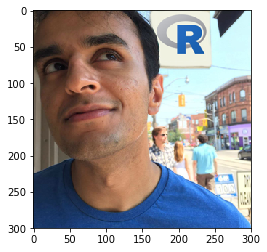
\includegraphics{output_9_0.png}
\caption{png}
\end{figure}

\begin{figure}
\centering
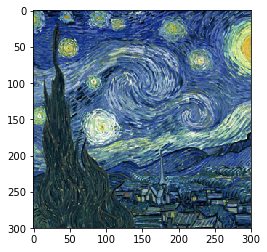
\includegraphics{output_9_1.png}
\caption{png}
\end{figure}

\section{Optimizing the loss}\label{optimizing-the-loss}

Now we are finally ready to find the image that minimizes the loss we
defined. We will use the optimization package in scipy and in particular
the LBFGS method. LBFGS is a great optimization procedure which is very
popular when computing the full gradient is feasible as is the case
here.

Notice that we are computing the gradient with respect to the input.
This is quite different from most other use cases where we compute the
gradient with respect to the network parameters. By default, input
variables do not ask for gradients, however we defined our input
variable as

\begin{Shaded}
\begin{Highlighting}[]
\NormalTok{y }\OperatorTok{=}\NormalTok{ C.input_variable((}\DecValTok{3}\NormalTok{, SIZE, SIZE), needs_gradient}\OperatorTok{=}\VariableTok{True}\NormalTok{)}
\end{Highlighting}
\end{Shaded}

which means that CNTK will compute the gradient with respect to this
input variable as well.

The rest of the code is straightforward and most of the complexity comes
from interacting with the scipy optimization package: - The optimizer
works only with vectors of double precision so img2vec takes a
(3,SIZE,SIZE) image and converts it to a vector of doubles - CNTK needs
the input as an image but scipy is calling us back with a vector - CNTK
computes a gradient as an image but scipy wants the gradient as a vector

Besides these complexities we just start from the content image (or a
random image), perform our optimization and display the final result.

\begin{Shaded}
\begin{Highlighting}[]
\CommentTok{# utility to convert a vector to an image}
\KeywordTok{def}\NormalTok{ vec2img(x):}
\NormalTok{    d }\OperatorTok{=}\NormalTok{ np.}\BuiltInTok{round}\NormalTok{(np.sqrt(x.size }\OperatorTok{/} \DecValTok{3}\NormalTok{)).astype(}\StringTok{'i'}\NormalTok{)}
    \ControlFlowTok{return}\NormalTok{ np.reshape(x.astype(np.float32), (}\DecValTok{3}\NormalTok{, d, d))}

\CommentTok{# utility to convert an image to a vector}
\KeywordTok{def}\NormalTok{ img2vec(img):}
    \ControlFlowTok{return}\NormalTok{ img.flatten().astype(np.float64)}

\CommentTok{# utility to compute the value and the gradient of f at a particular place defined by binding}
\KeywordTok{def}\NormalTok{ value_and_grads(f, binding):}
    \ControlFlowTok{if} \BuiltInTok{len}\NormalTok{(f.outputs) }\OperatorTok{!=} \DecValTok{1}\NormalTok{:}
        \ControlFlowTok{raise} \PreprocessorTok{ValueError}\NormalTok{(}\StringTok{'function must return a single tensor'}\NormalTok{)}
\NormalTok{    df, valdict }\OperatorTok{=}\NormalTok{ f.forward(binding, [f.output], }\BuiltInTok{set}\NormalTok{([f.output]))}
\NormalTok{    value }\OperatorTok{=} \BuiltInTok{list}\NormalTok{(valdict.values())[}\DecValTok{0}\NormalTok{]}
\NormalTok{    grads }\OperatorTok{=}\NormalTok{ f.backward(df, \{f.output: np.ones_like(value)\}, }\BuiltInTok{set}\NormalTok{(binding.keys()))}
    \ControlFlowTok{return}\NormalTok{ value, grads}

\CommentTok{# an objective function that scipy will be happy with}
\KeywordTok{def}\NormalTok{ objfun(x, loss):}
\NormalTok{    y }\OperatorTok{=}\NormalTok{ vec2img(x)}
\NormalTok{    v, g }\OperatorTok{=}\NormalTok{ value_and_grads(loss, \{loss.arguments[}\DecValTok{0}\NormalTok{]: [[y]]\})}
\NormalTok{    v }\OperatorTok{=}\NormalTok{ np.reshape(v, (}\DecValTok{1}\NormalTok{,))}
\NormalTok{    g }\OperatorTok{=}\NormalTok{ img2vec(}\BuiltInTok{list}\NormalTok{(g.values())[}\DecValTok{0}\NormalTok{])}
    \ControlFlowTok{return}\NormalTok{ v, g}

\CommentTok{# the actual optimization procedure}
\KeywordTok{def}\NormalTok{ optimize(loss, x0, inner, outer):}
\NormalTok{    bounds }\OperatorTok{=}\NormalTok{ [(}\OperatorTok{-}\NormalTok{np.}\BuiltInTok{min}\NormalTok{(SHIFT), }\DecValTok{255}\OperatorTok{-}\NormalTok{np.}\BuiltInTok{max}\NormalTok{(SHIFT))]}\OperatorTok{*}\NormalTok{x0.size}
    \ControlFlowTok{for}\NormalTok{ i }\KeywordTok{in} \BuiltInTok{range}\NormalTok{(outer):}
\NormalTok{        s }\OperatorTok{=}\NormalTok{ opt.minimize(objfun, img2vec(x0), args}\OperatorTok{=}\NormalTok{(loss,), method}\OperatorTok{=}\StringTok{'L-BFGS-B'}\NormalTok{, }
\NormalTok{                         bounds}\OperatorTok{=}\NormalTok{bounds, options}\OperatorTok{=}\NormalTok{\{}\StringTok{'maxiter'}\NormalTok{: inner\}, jac}\OperatorTok{=}\VariableTok{True}\NormalTok{)}
        \BuiltInTok{print}\NormalTok{(}\StringTok{'objective : }\SpecialCharTok\NormalTok{ s.fun[}\DecValTok{0}\NormalTok{])}
\NormalTok{        x0 }\OperatorTok{=}\NormalTok{ vec2img(s.x)}
\NormalTok{        path }\OperatorTok{=} \StringTok{'output_}\SpecialCharTok\NormalTok{ i}
\NormalTok{        save_image(x0, path)}
    \ControlFlowTok{return}\NormalTok{ x0}

\NormalTok{np.random.seed(}\DecValTok{98052}\NormalTok{)}
\ControlFlowTok{if}\NormalTok{ start_from_random:}
\NormalTok{    x0 }\OperatorTok{=}\NormalTok{ np.random.randn(}\DecValTok{3}\NormalTok{, SIZE, SIZE).astype(np.float32)}
\ControlFlowTok{else}\NormalTok{:}
\NormalTok{    x0 }\OperatorTok{=}\NormalTok{ content}
\NormalTok{xstar }\OperatorTok{=}\NormalTok{ optimize(loss, x0, inner, outer)}
\NormalTok{plt.imshow(np.asarray(np.transpose(xstar}\OperatorTok{+}\NormalTok{SHIFT, (}\DecValTok{1}\NormalTok{, }\DecValTok{2}\NormalTok{, }\DecValTok{0}\NormalTok{)), dtype}\OperatorTok{=}\NormalTok{np.uint8))}
\end{Highlighting}
\end{Shaded}

\begin{verbatim}
objective : 70194.4
objective : 60445.3
objective : 57855.2
objective : 56728.0
objective : 56166.7
objective : 55840.4
objective : 55627.4
objective : 55493.8
objective : 55395.1
objective : 55325.0





<matplotlib.image.AxesImage at 0x7fe962aa0e10>
\end{verbatim}

\begin{figure}
\centering
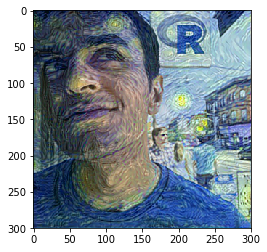
\includegraphics{output_11_2.png}
\caption{png}
\end{figure}

\begin{Shaded}
\begin{Highlighting}[]
\CommentTok{# For testing purposes}
\NormalTok{objfun(xstar, loss)[}\DecValTok{0}\NormalTok{][}\DecValTok{0}\NormalTok{]}
\end{Highlighting}
\end{Shaded}

\begin{verbatim}
55325.039
\end{verbatim}

\chapter{Network Visualization
(TensorFlow)}\label{network-visualization-tensorflow}

\emph{\textbf{Credit}: This notebook was derived from a homework
assignment in CS231N, taught in 2017 by Justin Johnson, Fei Fei Li, and
Serena Yeung}

In this notebook we will explore the use of \emph{image gradients} for
generating new images.

When training a model, we define a loss function which measures our
current unhappiness with the model's performance; we then use
backpropagation to compute the gradient of the loss with respect to the
model parameters, and perform gradient descent on the model parameters
to minimize the loss.

Here we will do something slightly different. We will start from a
convolutional neural network model which has been pretrained to perform
image classification on the ImageNet dataset. We will use this model to
define a loss function which quantifies our current unhappiness with our
image, then use backpropagation to compute the gradient of this loss
with respect to the pixels of the image. We will then keep the model
fixed, and perform gradient descent \emph{on the image} to synthesize a
new image which minimizes the loss.

In this notebook we will explore three techniques for image generation:

\begin{enumerate}
\def\labelenumi{\arabic{enumi}.}
\tightlist
\item
  \textbf{Saliency Maps}: Saliency maps are a quick way to tell which
  part of the image influenced the classification decision made by the
  network.
\item
  \textbf{Fooling Images}: We can perturb an input image so that it
  appears the same to humans, but will be misclassified by the
  pretrained network.
\item
  \textbf{Class Visualization}: We can synthesize an image to maximize
  the classification score of a particular class; this can give us some
  sense of what the network is looking for when it classifies images of
  that class.
\end{enumerate}

\begin{Shaded}
\begin{Highlighting}[]
\CommentTok{# As usual, a bit of setup}
\ImportTok{from}\NormalTok{ __future__ }\ImportTok{import}\NormalTok{ print_function}
\ImportTok{import}\NormalTok{ subprocess}
\ImportTok{import}\NormalTok{ time, os, json}
\ImportTok{import}\NormalTok{ numpy }\ImportTok{as}\NormalTok{ np}
\ImportTok{import}\NormalTok{ matplotlib.pyplot }\ImportTok{as}\NormalTok{ plt}
\ImportTok{import}\NormalTok{ tensorflow }\ImportTok{as}\NormalTok{ tf}

\ImportTok{from}\NormalTok{ utils.classifiers.squeezenet }\ImportTok{import}\NormalTok{ SqueezeNet}
\ImportTok{from}\NormalTok{ utils.data_utils }\ImportTok{import}\NormalTok{ load_tiny_imagenet}
\ImportTok{from}\NormalTok{ utils.image_utils }\ImportTok{import}\NormalTok{ preprocess_image, deprocess_image}
\ImportTok{from}\NormalTok{ utils.image_utils }\ImportTok{import}\NormalTok{ SQUEEZENET_MEAN, SQUEEZENET_STD}


\OperatorTok{%}\NormalTok{matplotlib inline}
\NormalTok{plt.rcParams[}\StringTok{'figure.figsize'}\NormalTok{] }\OperatorTok{=}\NormalTok{ (}\FloatTok{10.0}\NormalTok{, }\FloatTok{8.0}\NormalTok{) }\CommentTok{# set default size of plots}
\NormalTok{plt.rcParams[}\StringTok{'image.interpolation'}\NormalTok{] }\OperatorTok{=} \StringTok{'nearest'}
\NormalTok{plt.rcParams[}\StringTok{'image.cmap'}\NormalTok{] }\OperatorTok{=} \StringTok{'gray'}

\KeywordTok{def}\NormalTok{ get_session():}
    \CommentTok{"""Create a session that dynamically allocates memory."""}
    \CommentTok{# See: https://www.tensorflow.org/tutorials/using_gpu#allowing_gpu_memory_growth}
\NormalTok{    config }\OperatorTok{=}\NormalTok{ tf.ConfigProto()}
\NormalTok{    config.gpu_options.allow_growth }\OperatorTok{=} \VariableTok{True}
\NormalTok{    session }\OperatorTok{=}\NormalTok{ tf.Session(config}\OperatorTok{=}\NormalTok{config)}
    \ControlFlowTok{return}\NormalTok{ session}

\CommentTok{# for auto-reloading external modules}
\CommentTok{# see http://stackoverflow.com/questions/1907993/autoreload-of-modules-in-ipython}
\OperatorTok\NormalTok{autoreload }\DecValTok{2}
\end{Highlighting}
\end{Shaded}

\chapter{Pretrained Model}\label{pretrained-model}

For all of our image generation experiments, we will start with a
convolutional neural network which was pretrained to perform image
classification on ImageNet. We can use any model here, but for the
purposes of this assignment we will use SqueezeNet {[}1{]}, which
achieves accuracies comparable to AlexNet but with a significantly
reduced parameter count and computational complexity.

Using SqueezeNet rather than AlexNet or VGG or ResNet means that we can
easily perform all image generation experiments on CPU.

We have ported the PyTorch SqueezeNet model to TensorFlow; see:
\texttt{utils/classifiers/squeezenet.py} for the model architecture.

To use SqueezeNet, you will need to first \textbf{download the weights}
by changing into the \texttt{utils/datasets} directory and running
\texttt{get\_squeezenet\_tf.sh}. Note that if you ran
\texttt{get\_data.sh} then SqueezeNet will already be downloaded.

Once you've downloaded the Squeezenet model, we can load it into a new
TensorFlow session:

{[}1{]} {[}Iandola et al, ``SqueezeNet: AlexNet-level accuracy with 50x
fewer parameters and \textless{} 0.5MB model size'', arXiv
2016{]}(\url{https://arxiv.org/abs/1602.07360})

\begin{Shaded}
\begin{Highlighting}[]
\NormalTok{os.getcwd()}
\end{Highlighting}
\end{Shaded}

\begin{verbatim}
'/datadrive/az-courses/learnanalytics-deeplearning-azure/Students/10-adversarial-attacks/tensorflow'
\end{verbatim}

\begin{Shaded}
\begin{Highlighting}[]
\CommentTok{# %%bash}
\CommentTok{# cd utils/datasets}
\CommentTok{# chmod +x *.sh}
\CommentTok{# ./get_data.sh}
\end{Highlighting}
\end{Shaded}

\begin{Shaded}
\begin{Highlighting}[]
\NormalTok{tf.reset_default_graph()}
\NormalTok{sess }\OperatorTok{=}\NormalTok{ get_session()}

\NormalTok{SAVE_PATH }\OperatorTok{=} \StringTok{'utils/datasets/squeezenet.ckpt'}
\CommentTok{# if not os.path.exists(SAVE_PATH):}
\CommentTok{#     raise ValueError("You need to download SqueezeNet!")}
\NormalTok{model }\OperatorTok{=}\NormalTok{ SqueezeNet(save_path}\OperatorTok{=}\NormalTok{SAVE_PATH, sess}\OperatorTok{=}\NormalTok{sess)}
\end{Highlighting}
\end{Shaded}

\begin{verbatim}
INFO:tensorflow:Restoring parameters from utils/datasets/squeezenet.ckpt
\end{verbatim}

\section{Load some ImageNet images}\label{load-some-imagenet-images}

We have provided a few example images from the validation set of the
ImageNet ILSVRC 2012 Classification dataset. To download these images,
change to \texttt{utils/datasets/} and run
\texttt{get\_imagenet\_val.sh}.

Since they come from the validation set, our pretrained model did not
see these images during training.

Run the following cell to visualize some of these images, along with
their ground-truth labels.

\begin{Shaded}
\begin{Highlighting}[]
\ImportTok{from}\NormalTok{ utils.data_utils }\ImportTok{import}\NormalTok{ load_imagenet_val}
\NormalTok{X_raw, y, class_names }\OperatorTok{=}\NormalTok{ load_imagenet_val(num}\OperatorTok{=}\DecValTok{5}\NormalTok{)}

\NormalTok{plt.figure(figsize}\OperatorTok{=}\NormalTok{(}\DecValTok{12}\NormalTok{, }\DecValTok{6}\NormalTok{))}
\ControlFlowTok{for}\NormalTok{ i }\KeywordTok{in} \BuiltInTok{range}\NormalTok{(}\DecValTok{5}\NormalTok{):}
\NormalTok{    plt.subplot(}\DecValTok{1}\NormalTok{, }\DecValTok{5}\NormalTok{, i }\OperatorTok{+} \DecValTok{1}\NormalTok{)}
\NormalTok{    plt.imshow(X_raw[i])}
\NormalTok{    plt.title(class_names[y[i]])}
\NormalTok{    plt.axis(}\StringTok{'off'}\NormalTok{)}
\NormalTok{plt.gcf().tight_layout()}
\end{Highlighting}
\end{Shaded}

\begin{figure}
\centering
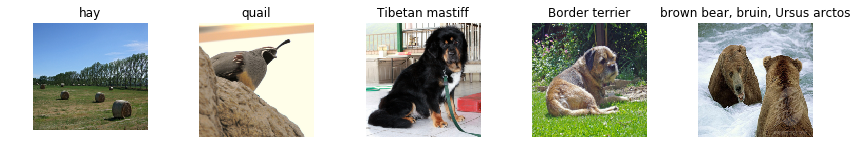
\includegraphics{Network-Visualization-TensorFlow_files/Network-Visualization-TensorFlow_7_0.png}
\caption{png}
\end{figure}

\section{Preprocess images}\label{preprocess-images}

The input to the pretrained model is expected to be normalized, so we
first preprocess the images by subtracting the pixelwise mean and
dividing by the pixelwise standard deviation.

\begin{Shaded}
\begin{Highlighting}[]
\NormalTok{X }\OperatorTok{=}\NormalTok{ np.array([preprocess_image(img) }\ControlFlowTok{for}\NormalTok{ img }\KeywordTok{in}\NormalTok{ X_raw])}
\end{Highlighting}
\end{Shaded}

\chapter{Saliency Maps}\label{saliency-maps}

Using this pretrained model, we will compute class saliency maps as
described in Section 3.1 of {[}2{]}.

A \textbf{saliency map} tells us the degree to which each pixel in the
image affects the classification score for that image. To compute it, we
compute the gradient of the unnormalized score corresponding to the
correct class (which is a scalar) with respect to the pixels of the
image. If the image has shape \texttt{(H,\ W,\ 3)} then this gradient
will also have shape \texttt{(H,\ W,\ 3)}; for each pixel in the image,
this gradient tells us the amount by which the classification score will
change if the pixel changes by a small amount. To compute the saliency
map, we take the absolute value of this gradient, then take the maximum
value over the 3 input channels; the final saliency map thus has shape
\texttt{(H,\ W)} and all entries are nonnegative.

You will need to use the \texttt{model.classifier} Tensor containing the
scores for each input, and will need to feed in values for the
\texttt{model.image} and \texttt{model.labels} placeholder when
evaluating the gradient. Open the file
\texttt{utils/classifiers/squeezenet.py} and read the documentation to
make sure you understand how to use the model. For example usage, you
can see the \texttt{loss} attribute.

{[}2{]} {[}Karen Simonyan, Andrea Vedaldi, and Andrew Zisserman. ``Deep
Inside Convolutional Networks: Visualising Image Classification Models
and Saliency Maps'', ICLR Workshop
2014{]}(\url{https://arxiv.org/abs/1312.6034}).

\begin{Shaded}
\begin{Highlighting}[]
\KeywordTok{def}\NormalTok{ compute_saliency_maps(X, y, model):}
    \CommentTok{"""}
\CommentTok{    Compute a class saliency map using the model for images X and labels y.}

\CommentTok{    Input:}
\CommentTok{    - X: Input images, numpy array of shape (N, H, W, 3)}
\CommentTok{    - y: Labels for X, numpy of shape (N,)}
\CommentTok{    - model: A SqueezeNet model that will be used to compute the saliency map.}

\CommentTok{    Returns:}
\CommentTok{    - saliency: A numpy array of shape (N, H, W) giving the saliency maps for the}
\CommentTok{    input images.}
\CommentTok{    """}
\NormalTok{    saliency }\OperatorTok{=} \VariableTok{None}
    \CommentTok{# Compute the score of the correct class for each example.}
    \CommentTok{# This gives a Tensor with shape [N], the number of examples.}
    \CommentTok{#}
    \CommentTok{# Note: this is equivalent to scores[np.arange(N), y] we used in NumPy}
    \CommentTok{# for computing vectorized losses.}
\NormalTok{    correct_scores }\OperatorTok{=}\NormalTok{ tf.gather_nd(model.classifier,}
\NormalTok{                                  tf.stack((tf.}\BuiltInTok{range}\NormalTok{(X.shape[}\DecValTok{0}\NormalTok{]), model.labels), axis}\OperatorTok{=}\DecValTok{1}\NormalTok{))}
    \CommentTok{###############################################################################}
    \CommentTok{# }\AlertTok{TODO}\CommentTok{: Implement this function. You should use the correct_scores to compute #}
    \CommentTok{# the loss, and tf.gradients to compute the gradient of the loss with respect #}
    \CommentTok{# to the input image stored in model.image.                                   #}
    \CommentTok{# Use the global sess variable to finally run the computation.                #}
    \CommentTok{# Note: model.image and model.labels are placeholders and must be fed values  #}
    \CommentTok{# when you call sess.run().                                                   #}
    \CommentTok{###############################################################################}
\NormalTok{    grad }\OperatorTok{=}\NormalTok{ tf.gradients(correct_scores, model.image)[}\DecValTok{0}\NormalTok{]}
\NormalTok{    grad_val }\OperatorTok{=}\NormalTok{ sess.run(grad, \{model.image: X, }
\NormalTok{                               model.labels: y\})}
\NormalTok{    saliency }\OperatorTok{=}\NormalTok{ np.}\BuiltInTok{max}\NormalTok{(np.absolute(grad_val), axis}\OperatorTok{=}\DecValTok{3}\NormalTok{)}
    \CommentTok{##############################################################################}
    \CommentTok{#                             }\RegionMarkerTok{END}\CommentTok{ OF YOUR CODE                               #}
    \CommentTok{##############################################################################}
    \ControlFlowTok{return}\NormalTok{ saliency}
\end{Highlighting}
\end{Shaded}

Once you have completed the implementation in the cell above, run the
following to visualize some class saliency maps on our example images
from the ImageNet validation set:

\begin{Shaded}
\begin{Highlighting}[]
\KeywordTok{def}\NormalTok{ show_saliency_maps(X, y, mask):}
\NormalTok{    mask }\OperatorTok{=}\NormalTok{ np.asarray(mask)}
\NormalTok{    Xm }\OperatorTok{=}\NormalTok{ X[mask]}
\NormalTok{    ym }\OperatorTok{=}\NormalTok{ y[mask]}

\NormalTok{    saliency }\OperatorTok{=}\NormalTok{ compute_saliency_maps(Xm, ym, model)}

    \ControlFlowTok{for}\NormalTok{ i }\KeywordTok{in} \BuiltInTok{range}\NormalTok{(mask.size):}
\NormalTok{        plt.subplot(}\DecValTok{2}\NormalTok{, mask.size, i }\OperatorTok{+} \DecValTok{1}\NormalTok{)}
\NormalTok{        plt.imshow(deprocess_image(Xm[i]))}
\NormalTok{        plt.axis(}\StringTok{'off'}\NormalTok{)}
\NormalTok{        plt.title(class_names[ym[i]])}
\NormalTok{        plt.subplot(}\DecValTok{2}\NormalTok{, mask.size, mask.size }\OperatorTok{+}\NormalTok{ i }\OperatorTok{+} \DecValTok{1}\NormalTok{)}
\NormalTok{        plt.title(mask[i])}
\NormalTok{        plt.imshow(saliency[i], cmap}\OperatorTok{=}\NormalTok{plt.cm.hot)}
\NormalTok{        plt.axis(}\StringTok{'off'}\NormalTok{)}
\NormalTok{        plt.gcf().set_size_inches(}\DecValTok{10}\NormalTok{, }\DecValTok{4}\NormalTok{)}
\NormalTok{    plt.show()}

\NormalTok{mask }\OperatorTok{=}\NormalTok{ np.arange(}\DecValTok{5}\NormalTok{)}
\NormalTok{show_saliency_maps(X, y, mask)}
\end{Highlighting}
\end{Shaded}

\begin{figure}
\centering
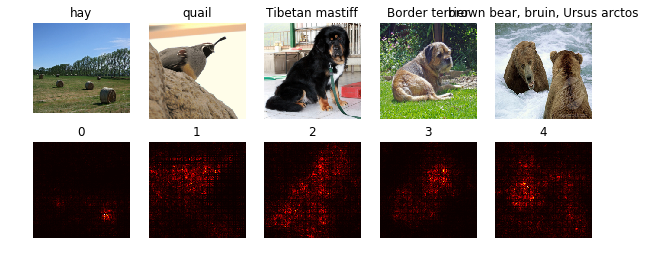
\includegraphics{Network-Visualization-TensorFlow_files/Network-Visualization-TensorFlow_13_0.png}
\caption{png}
\end{figure}

\chapter{Fooling Images}\label{fooling-images}

We can also use image gradients to generate ``fooling images'' as
discussed in {[}3{]}. Given an image and a target class, we can perform
gradient \textbf{ascent} over the image to maximize the target class,
stopping when the network classifies the image as the target class.
Implement the following function to generate fooling images.

{[}3{]} {[}Szegedy et al, ``Intriguing properties of neural networks'',
ICLR 2014{]}(\url{https://arxiv.org/abs/1312.6199})

\begin{Shaded}
\begin{Highlighting}[]
\KeywordTok{def}\NormalTok{ make_fooling_image(X, target_y, model):}
    \CommentTok{"""}
\CommentTok{    Generate a fooling image that is close to X, but that the model classifies}
\CommentTok{    as target_y.}

\CommentTok{    Inputs:}
\CommentTok{    - X: Input image, of shape (1, 224, 224, 3)}
\CommentTok{    - target_y: An integer in the range [0, 1000)}
\CommentTok{    - model: Pretrained SqueezeNet model}

\CommentTok{    Returns:}
\CommentTok{    - X_fooling: An image that is close to X, but that is classifed as target_y}
\CommentTok{    by the model.}
\CommentTok{    """}
\NormalTok{    X_fooling }\OperatorTok{=}\NormalTok{ X.copy()}
\NormalTok{    learning_rate }\OperatorTok{=} \DecValTok{1}
    \CommentTok{##############################################################################}
    \CommentTok{# }\AlertTok{TODO}\CommentTok{: Generate a fooling image X_fooling that the model will classify as   #}
    \CommentTok{# the class target_y. Use gradient ascent on the target class score, using   #}
    \CommentTok{# the model.classifier Tensor to get the class scores for the model.image.   #}
    \CommentTok{# When computing an update step, first normalize the gradient:               #}
    \CommentTok{#   dX = learning_rate * g / ||g||_2                                         #}
    \CommentTok{#                                                                            #}
    \CommentTok{# You should write a training loop                                           #}
    \CommentTok{#                                                                            #  }
    \CommentTok{# HINT: For most examples, you should be able to generate a fooling image    #}
    \CommentTok{# in fewer than 100 iterations of gradient ascent.                           #}
    \CommentTok{# You can print your progress over iterations to check your algorithm.       #}
    \CommentTok{##############################################################################}
\NormalTok{    iterations }\OperatorTok{=} \DecValTok{100}
\NormalTok{    loss }\OperatorTok{=}\NormalTok{ model.classifier[}\DecValTok{0}\NormalTok{][target_y]}
\NormalTok{    grad }\OperatorTok{=}\NormalTok{ tf.gradients(loss, model.image)[}\DecValTok{0}\NormalTok{]}
    
    \ControlFlowTok{for}\NormalTok{ i }\KeywordTok{in} \BuiltInTok{range}\NormalTok{(iterations):}
\NormalTok{        scores }\OperatorTok{=}\NormalTok{ sess.run(model.classifier, feed_dict}\OperatorTok{=}\NormalTok{\{model.image: X_fooling\})}
\NormalTok{        g }\OperatorTok{=}\NormalTok{ sess.run(grad, feed_dict}\OperatorTok{=}\NormalTok{\{model.image: X_fooling\})}
\NormalTok{        target_i }\OperatorTok{=}\NormalTok{ np.argmax(scores[}\DecValTok{0}\NormalTok{])}
        \ControlFlowTok{if}\NormalTok{ target_i }\OperatorTok{==}\NormalTok{ target_y:}
            \ControlFlowTok{break}\OperatorTok{;}
        \ControlFlowTok{else}\NormalTok{:}
\NormalTok{            dX }\OperatorTok{=}\NormalTok{ learning_rate }\OperatorTok{*}\NormalTok{ g }\OperatorTok{/}\NormalTok{ np.sqrt(np.}\BuiltInTok{sum}\NormalTok{(g}\OperatorTok{*}\NormalTok{g))}
\NormalTok{            X_fooling }\OperatorTok{+=}\NormalTok{ dX}
    \CommentTok{##############################################################################}
    \CommentTok{#                             }\RegionMarkerTok{END}\CommentTok{ OF YOUR CODE                               #}
    \CommentTok{##############################################################################}
    \ControlFlowTok{return}\NormalTok{ X_fooling}
\end{Highlighting}
\end{Shaded}

Run the following to generate a fooling image. Feel free to change the
\texttt{idx} variable to explore other images.

\begin{Shaded}
\begin{Highlighting}[]
\NormalTok{idx }\OperatorTok{=} \DecValTok{2}
\NormalTok{Xi }\OperatorTok{=}\NormalTok{ X[idx][}\VariableTok{None}\NormalTok{]}
\NormalTok{target_y }\OperatorTok{=} \DecValTok{9}
\NormalTok{X_fooling }\OperatorTok{=}\NormalTok{ make_fooling_image(Xi, target_y, model)}

\CommentTok{# Make sure that X_fooling is classified as y_target}
\NormalTok{scores }\OperatorTok{=}\NormalTok{ sess.run(model.classifier, \{model.image: X_fooling\})}
\ControlFlowTok{assert}\NormalTok{ scores[}\DecValTok{0}\NormalTok{].argmax() }\OperatorTok{==}\NormalTok{ target_y, }\StringTok{'The network is not fooled!'}

\CommentTok{# Show original image, fooling image, and difference}
\NormalTok{orig_img }\OperatorTok{=}\NormalTok{ deprocess_image(Xi[}\DecValTok{0}\NormalTok{])}
\NormalTok{fool_img }\OperatorTok{=}\NormalTok{ deprocess_image(X_fooling[}\DecValTok{0}\NormalTok{])}
\CommentTok{# Rescale }
\NormalTok{plt.subplot(}\DecValTok{1}\NormalTok{, }\DecValTok{4}\NormalTok{, }\DecValTok{1}\NormalTok{)}
\NormalTok{plt.imshow(orig_img)}
\NormalTok{plt.axis(}\StringTok{'off'}\NormalTok{)}
\NormalTok{plt.title(class_names[y[idx]])}
\NormalTok{plt.subplot(}\DecValTok{1}\NormalTok{, }\DecValTok{4}\NormalTok{, }\DecValTok{2}\NormalTok{)}
\NormalTok{plt.imshow(fool_img)}
\NormalTok{plt.title(class_names[target_y])}
\NormalTok{plt.axis(}\StringTok{'off'}\NormalTok{)}
\NormalTok{plt.subplot(}\DecValTok{1}\NormalTok{, }\DecValTok{4}\NormalTok{, }\DecValTok{3}\NormalTok{)}
\NormalTok{plt.title(}\StringTok{'Difference'}\NormalTok{)}
\NormalTok{plt.imshow(deprocess_image((Xi}\OperatorTok{-}\NormalTok{X_fooling)[}\DecValTok{0}\NormalTok{]))}
\NormalTok{plt.axis(}\StringTok{'off'}\NormalTok{)}
\NormalTok{plt.subplot(}\DecValTok{1}\NormalTok{, }\DecValTok{4}\NormalTok{, }\DecValTok{4}\NormalTok{)}
\NormalTok{plt.title(}\StringTok{'Magnified difference (10x)'}\NormalTok{)}
\NormalTok{plt.imshow(deprocess_image(}\DecValTok{10} \OperatorTok{*}\NormalTok{ (Xi}\OperatorTok{-}\NormalTok{X_fooling)[}\DecValTok{0}\NormalTok{]))}
\NormalTok{plt.axis(}\StringTok{'off'}\NormalTok{)}
\NormalTok{plt.gcf().tight_layout()}
\end{Highlighting}
\end{Shaded}

\begin{figure}
\centering
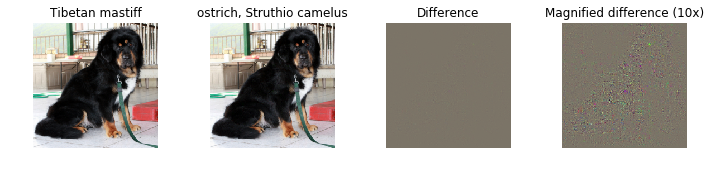
\includegraphics{Network-Visualization-TensorFlow_files/Network-Visualization-TensorFlow_17_0.png}
\caption{png}
\end{figure}

\paragraph{Class visualization}\label{class-visualization}

By starting with a random noise image and performing gradient ascent on
a target class, we can generate an image that the network will recognize
as the target class. This idea was first presented in {[}2{]}; {[}3{]}
extended this idea by suggesting several regularization techniques that
can improve the quality of the generated image.

Concretely, let \(I\) be an image and let \(y\) be a target class. Let
\(s_y(I)\) be the score that a convolutional network assigns to the
image \(I\) for class \(y\); note that these are raw unnormalized
scores, not class probabilities. We wish to generate an image \(I^*\)
that achieves a high score for the class \(y\) by solving the problem

\[
I^* = \arg\max_I s_y(I) - R(I)
\]

where \(R\) is a (possibly implicit) regularizer (note the sign of
\(R(I)\) in the argmax: we want to minimize this regularization term).
We can solve this optimization problem using gradient ascent, computing
gradients with respect to the generated image. We will use (explicit) L2
regularization of the form

\[
R(I) = \lambda \|I\|_2^2
\]

\textbf{and} implicit regularization as suggested by {[}3{]} by
periodically blurring the generated image. We can solve this problem
using gradient ascent on the generated image.

In the cell below, complete the implementation of the
\texttt{create\_class\_visualization} function.

{[}2{]} {[}Karen Simonyan, Andrea Vedaldi, and Andrew Zisserman. ``Deep
Inside Convolutional Networks: Visualising Image Classification Models
and Saliency Maps'', ICLR Workshop
2014{]}(\url{https://arxiv.org/abs/1312.6034}).

{[}3{]} {[}Yosinski et al, ``Understanding Neural Networks Through Deep
Visualization'', ICML 2015 Deep Learning
Workshop{]}(\url{https://arxiv.org/abs/1506.06579}).

\begin{Shaded}
\begin{Highlighting}[]
\ImportTok{from}\NormalTok{ scipy.ndimage.filters }\ImportTok{import}\NormalTok{ gaussian_filter1d}
\KeywordTok{def}\NormalTok{ blur_image(X, sigma}\OperatorTok{=}\DecValTok{1}\NormalTok{):}
\NormalTok{    X }\OperatorTok{=}\NormalTok{ gaussian_filter1d(X, sigma, axis}\OperatorTok{=}\DecValTok{1}\NormalTok{)}
\NormalTok{    X }\OperatorTok{=}\NormalTok{ gaussian_filter1d(X, sigma, axis}\OperatorTok{=}\DecValTok{2}\NormalTok{)}
    \ControlFlowTok{return}\NormalTok{ X}
\end{Highlighting}
\end{Shaded}

\begin{Shaded}
\begin{Highlighting}[]
\KeywordTok{def}\NormalTok{ create_class_visualization(target_y, model, }\OperatorTok{**}\NormalTok{kwargs):}
    \CommentTok{"""}
\CommentTok{    Generate an image to maximize the score of target_y under a pretrained model.}
\CommentTok{    }
\CommentTok{    Inputs:}
\CommentTok{    - target_y: Integer in the range [0, 1000) giving the index of the class}
\CommentTok{    - model: A pretrained CNN that will be used to generate the image}
\CommentTok{    }
\CommentTok{    Keyword arguments:}
\CommentTok{    - l2_reg: Strength of L2 regularization on the image}
\CommentTok{    - learning_rate: How big of a step to take}
\CommentTok{    - num_iterations: How many iterations to use}
\CommentTok{    - blur_every: How often to blur the image as an implicit regularizer}
\CommentTok{    - max_jitter: How much to gjitter the image as an implicit regularizer}
\CommentTok{    - show_every: How often to show the intermediate result}
\CommentTok{    """}
\NormalTok{    l2_reg }\OperatorTok{=}\NormalTok{ kwargs.pop(}\StringTok{'l2_reg'}\NormalTok{, }\FloatTok{1e-3}\NormalTok{)}
\NormalTok{    learning_rate }\OperatorTok{=}\NormalTok{ kwargs.pop(}\StringTok{'learning_rate'}\NormalTok{, }\DecValTok{25}\NormalTok{)}
\NormalTok{    num_iterations }\OperatorTok{=}\NormalTok{ kwargs.pop(}\StringTok{'num_iterations'}\NormalTok{, }\DecValTok{1000}\NormalTok{)}
\NormalTok{    blur_every }\OperatorTok{=}\NormalTok{ kwargs.pop(}\StringTok{'blur_every'}\NormalTok{, }\DecValTok{10}\NormalTok{)}
\NormalTok{    max_jitter }\OperatorTok{=}\NormalTok{ kwargs.pop(}\StringTok{'max_jitter'}\NormalTok{, }\DecValTok{1}\NormalTok{)}
\NormalTok{    show_every }\OperatorTok{=}\NormalTok{ kwargs.pop(}\StringTok{'show_every'}\NormalTok{, }\DecValTok{25}\NormalTok{)}

\NormalTok{    X }\OperatorTok{=} \DecValTok{255} \OperatorTok{*}\NormalTok{ np.random.rand(}\DecValTok{224}\NormalTok{, }\DecValTok{224}\NormalTok{, }\DecValTok{3}\NormalTok{)}
\NormalTok{    X }\OperatorTok{=}\NormalTok{ preprocess_image(X)[}\VariableTok{None}\NormalTok{]}
    
    \CommentTok{########################################################################}
    \CommentTok{# }\AlertTok{TODO}\CommentTok{: Compute the loss and the gradient of the loss with respect to  #}
    \CommentTok{# the input image, model.image. We compute these outside the loop so   #}
    \CommentTok{# that we don't have to recompute the gradient graph at each iteration #}
    \CommentTok{#                                                                      #}
    \CommentTok{# Note: loss and grad should be TensorFlow Tensors, not numpy arrays!  #}
    \CommentTok{#                                                                      #}
    \CommentTok{# The loss is the score for the target label, target_y. You should     #}
    \CommentTok{# use model.classifier to get the scores, and tf.gradients to compute  #}
    \CommentTok{# gradients. Don't forget the (subtracted) L2 regularization term!     #}
    \CommentTok{########################################################################}
\NormalTok{    loss }\OperatorTok{=} \VariableTok{None} \CommentTok{# scalar loss}
\NormalTok{    grad }\OperatorTok{=} \VariableTok{None} \CommentTok{# gradient of loss with respect to model.image, same size as model.image}
\NormalTok{    penalty }\OperatorTok{=}\NormalTok{ l2_reg }\OperatorTok{*}\NormalTok{ tf.norm(model.image)}
\NormalTok{    loss }\OperatorTok{=}\NormalTok{ model.classifier[}\DecValTok{0}\NormalTok{, target_y] }\OperatorTok{-}\NormalTok{ penalty}
\NormalTok{    grad }\OperatorTok{=}\NormalTok{ tf.gradients(loss, model.image)[}\DecValTok{0}\NormalTok{]}
    \CommentTok{############################################################################}
    \CommentTok{#                             }\RegionMarkerTok{END}\CommentTok{ OF YOUR CODE                             #}
    \CommentTok{############################################################################}

    
    \ControlFlowTok{for}\NormalTok{ t }\KeywordTok{in} \BuiltInTok{range}\NormalTok{(num_iterations):}
        \CommentTok{# Randomly jitter the image a bit; this gives slightly nicer results}
\NormalTok{        ox, oy }\OperatorTok{=}\NormalTok{ np.random.randint(}\OperatorTok{-}\NormalTok{max_jitter, max_jitter}\OperatorTok{+}\DecValTok{1}\NormalTok{, }\DecValTok{2}\NormalTok{)}
\NormalTok{        Xi }\OperatorTok{=}\NormalTok{ X.copy()}
\NormalTok{        X }\OperatorTok{=}\NormalTok{ np.roll(np.roll(X, ox, }\DecValTok{1}\NormalTok{), oy, }\DecValTok{2}\NormalTok{)}
        
        \CommentTok{########################################################################}
        \CommentTok{# }\AlertTok{TODO}\CommentTok{: Use sess to compute the value of the gradient of the score for #}
        \CommentTok{# class target_y with respect to the pixels of the image, and make a   #}
        \CommentTok{# gradient step on the image using the learning rate. You should use   #}
        \CommentTok{# the grad variable you defined above.                                 #}
        \CommentTok{#                                                                      #}
        \CommentTok{# Be very careful about the signs of elements in your code.            #}
        \CommentTok{########################################################################}
\NormalTok{        grad_val }\OperatorTok{=}\NormalTok{ sess.run(grad, \{model.image: X\})}
\NormalTok{        dX }\OperatorTok{=}\NormalTok{ learning_rate }\OperatorTok{*}\NormalTok{ grad_val}\OperatorTok{/}\NormalTok{np.linalg.norm(grad_val)}
\NormalTok{        X }\OperatorTok{+=}\NormalTok{ dX}
        \CommentTok{############################################################################}
        \CommentTok{#                             }\RegionMarkerTok{END}\CommentTok{ OF YOUR CODE                             #}
        \CommentTok{############################################################################}

        \CommentTok{# Undo the jitter}
\NormalTok{        X }\OperatorTok{=}\NormalTok{ np.roll(np.roll(X, }\OperatorTok{-}\NormalTok{ox, }\DecValTok{1}\NormalTok{), }\OperatorTok{-}\NormalTok{oy, }\DecValTok{2}\NormalTok{)}

        \CommentTok{# As a regularizer, clip and periodically blur}
\NormalTok{        X }\OperatorTok{=}\NormalTok{ np.clip(X, }\OperatorTok{-}\NormalTok{SQUEEZENET_MEAN}\OperatorTok{/}\NormalTok{SQUEEZENET_STD, (}\FloatTok{1.0} \OperatorTok{-}\NormalTok{ SQUEEZENET_MEAN)}\OperatorTok{/}\NormalTok{SQUEEZENET_STD)}
        \ControlFlowTok{if}\NormalTok{ t }\OperatorTok\NormalTok{ show_every }\OperatorTok{==} \DecValTok{0} \KeywordTok{or}\NormalTok{ t }\OperatorTok{==}\NormalTok{ num_iterations }\OperatorTok{-} \DecValTok{1}\NormalTok{:}
\NormalTok{            plt.imshow(deprocess_image(X[}\DecValTok{0}\NormalTok{]))}
\NormalTok{            class_name }\OperatorTok{=}\NormalTok{ class_names[target_y]}
\NormalTok{            plt.title(}\StringTok{'}\SpecialCharTok{%s}\CharTok{\textbackslash{}n}\StringTok{Iteration }\SpecialCharTok{%d}\StringTok{ / }\SpecialCharTok\NormalTok{ (class_name, t }\OperatorTok{+} \DecValTok{1}\NormalTok{, num_iterations))}
\NormalTok{            plt.gcf().set_size_inches(}\DecValTok{4}\NormalTok{, }\DecValTok{4}\NormalTok{)}
\NormalTok{            plt.axis(}\StringTok{'off'}\NormalTok{)}
\NormalTok{            plt.show()}
    \ControlFlowTok{return}\NormalTok{ X}
\end{Highlighting}
\end{Shaded}

Once you have completed the implementation in the cell above, run the
following cell to generate an image of Tarantula:

\begin{Shaded}
\begin{Highlighting}[]
\NormalTok{target_y }\OperatorTok{=} \DecValTok{7} \CommentTok{# Tarantula}
\NormalTok{out }\OperatorTok{=}\NormalTok{ create_class_visualization(target_y, model)}
\end{Highlighting}
\end{Shaded}

\begin{figure}
\centering
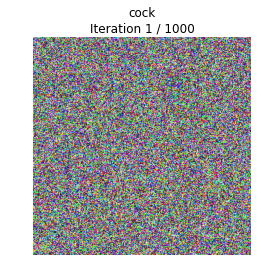
\includegraphics{Network-Visualization-TensorFlow_files/Network-Visualization-TensorFlow_22_0.png}
\caption{png}
\end{figure}

\begin{figure}
\centering
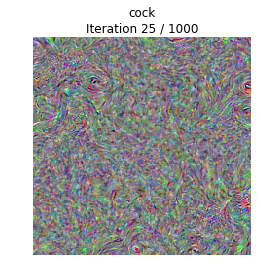
\includegraphics{Network-Visualization-TensorFlow_files/Network-Visualization-TensorFlow_22_1.png}
\caption{png}
\end{figure}

\begin{figure}
\centering
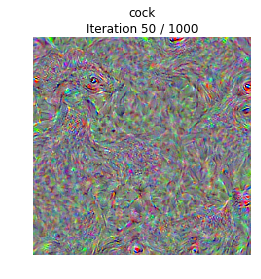
\includegraphics{Network-Visualization-TensorFlow_files/Network-Visualization-TensorFlow_22_2.png}
\caption{png}
\end{figure}

\begin{figure}
\centering
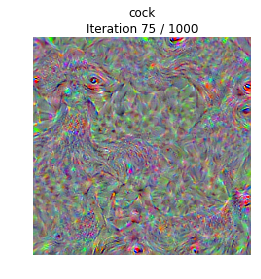
\includegraphics{Network-Visualization-TensorFlow_files/Network-Visualization-TensorFlow_22_3.png}
\caption{png}
\end{figure}

\begin{figure}
\centering
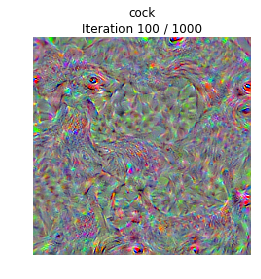
\includegraphics{Network-Visualization-TensorFlow_files/Network-Visualization-TensorFlow_22_4.png}
\caption{png}
\end{figure}

\begin{figure}
\centering
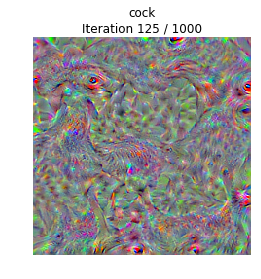
\includegraphics{Network-Visualization-TensorFlow_files/Network-Visualization-TensorFlow_22_5.png}
\caption{png}
\end{figure}

\begin{figure}
\centering
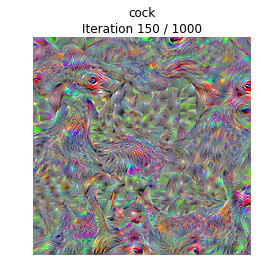
\includegraphics{Network-Visualization-TensorFlow_files/Network-Visualization-TensorFlow_22_6.png}
\caption{png}
\end{figure}

\begin{figure}
\centering
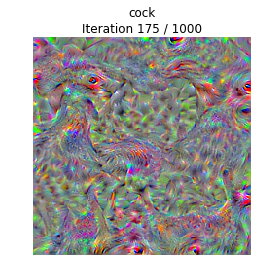
\includegraphics{Network-Visualization-TensorFlow_files/Network-Visualization-TensorFlow_22_7.png}
\caption{png}
\end{figure}

\begin{figure}
\centering
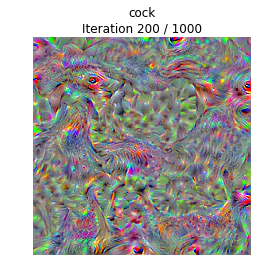
\includegraphics{Network-Visualization-TensorFlow_files/Network-Visualization-TensorFlow_22_8.png}
\caption{png}
\end{figure}

\begin{figure}
\centering
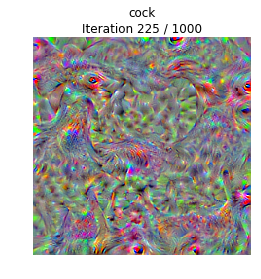
\includegraphics{Network-Visualization-TensorFlow_files/Network-Visualization-TensorFlow_22_9.png}
\caption{png}
\end{figure}

\begin{figure}
\centering
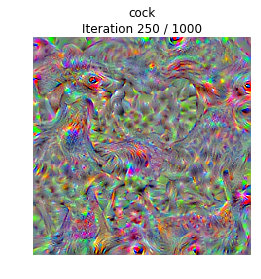
\includegraphics{Network-Visualization-TensorFlow_files/Network-Visualization-TensorFlow_22_10.png}
\caption{png}
\end{figure}

\begin{figure}
\centering
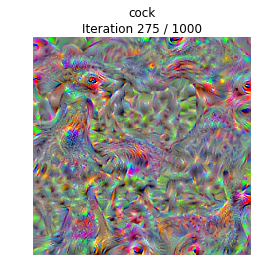
\includegraphics{Network-Visualization-TensorFlow_files/Network-Visualization-TensorFlow_22_11.png}
\caption{png}
\end{figure}

\begin{figure}
\centering
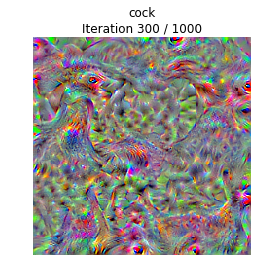
\includegraphics{Network-Visualization-TensorFlow_files/Network-Visualization-TensorFlow_22_12.png}
\caption{png}
\end{figure}

\begin{figure}
\centering
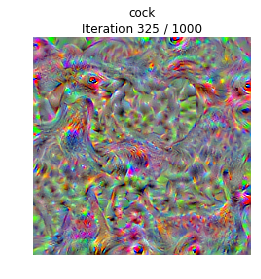
\includegraphics{Network-Visualization-TensorFlow_files/Network-Visualization-TensorFlow_22_13.png}
\caption{png}
\end{figure}

\begin{figure}
\centering
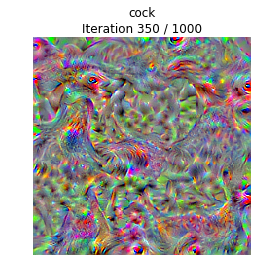
\includegraphics{Network-Visualization-TensorFlow_files/Network-Visualization-TensorFlow_22_14.png}
\caption{png}
\end{figure}

\begin{figure}
\centering
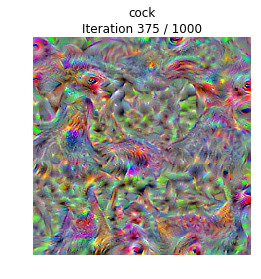
\includegraphics{Network-Visualization-TensorFlow_files/Network-Visualization-TensorFlow_22_15.png}
\caption{png}
\end{figure}

\begin{figure}
\centering
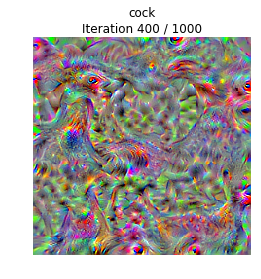
\includegraphics{Network-Visualization-TensorFlow_files/Network-Visualization-TensorFlow_22_16.png}
\caption{png}
\end{figure}

\begin{figure}
\centering
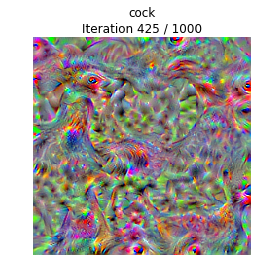
\includegraphics{Network-Visualization-TensorFlow_files/Network-Visualization-TensorFlow_22_17.png}
\caption{png}
\end{figure}

\begin{figure}
\centering
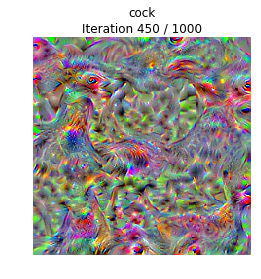
\includegraphics{Network-Visualization-TensorFlow_files/Network-Visualization-TensorFlow_22_18.png}
\caption{png}
\end{figure}

\begin{figure}
\centering
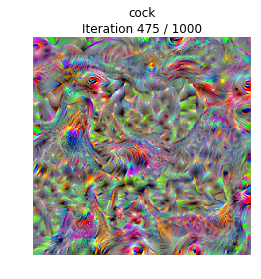
\includegraphics{Network-Visualization-TensorFlow_files/Network-Visualization-TensorFlow_22_19.png}
\caption{png}
\end{figure}

\begin{figure}
\centering
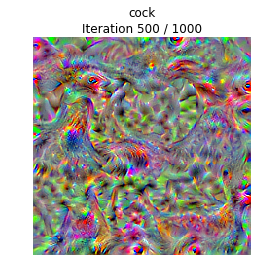
\includegraphics{Network-Visualization-TensorFlow_files/Network-Visualization-TensorFlow_22_20.png}
\caption{png}
\end{figure}

\begin{figure}
\centering
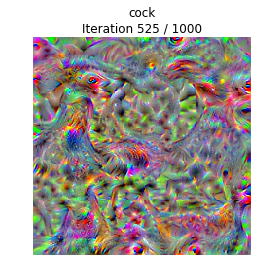
\includegraphics{Network-Visualization-TensorFlow_files/Network-Visualization-TensorFlow_22_21.png}
\caption{png}
\end{figure}

\begin{figure}
\centering
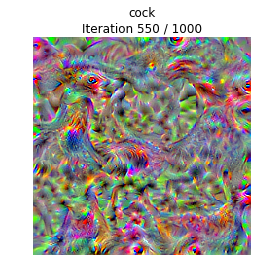
\includegraphics{Network-Visualization-TensorFlow_files/Network-Visualization-TensorFlow_22_22.png}
\caption{png}
\end{figure}

\begin{figure}
\centering
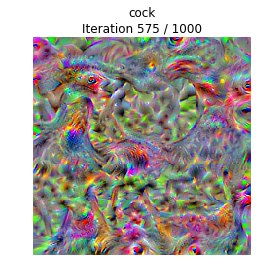
\includegraphics{Network-Visualization-TensorFlow_files/Network-Visualization-TensorFlow_22_23.png}
\caption{png}
\end{figure}

\begin{figure}
\centering
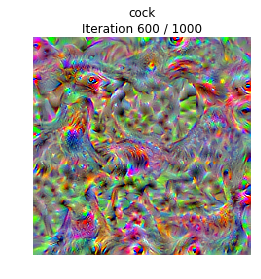
\includegraphics{Network-Visualization-TensorFlow_files/Network-Visualization-TensorFlow_22_24.png}
\caption{png}
\end{figure}

\begin{figure}
\centering
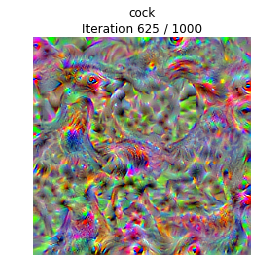
\includegraphics{Network-Visualization-TensorFlow_files/Network-Visualization-TensorFlow_22_25.png}
\caption{png}
\end{figure}

\begin{figure}
\centering
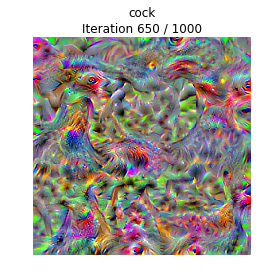
\includegraphics{Network-Visualization-TensorFlow_files/Network-Visualization-TensorFlow_22_26.png}
\caption{png}
\end{figure}

\begin{figure}
\centering
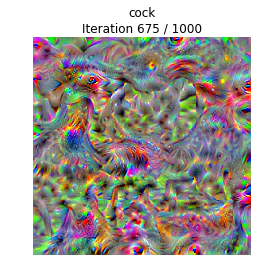
\includegraphics{Network-Visualization-TensorFlow_files/Network-Visualization-TensorFlow_22_27.png}
\caption{png}
\end{figure}

\begin{figure}
\centering
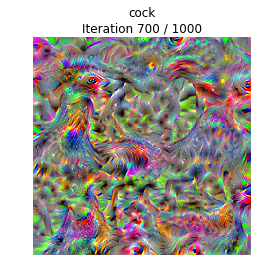
\includegraphics{Network-Visualization-TensorFlow_files/Network-Visualization-TensorFlow_22_28.png}
\caption{png}
\end{figure}

\begin{figure}
\centering
\includegraphics{Network-Visualization-TensorFlow_files/Network-Visualization-TensorFlow_22_29.png}
\caption{png}
\end{figure}

\begin{figure}
\centering
\includegraphics{Network-Visualization-TensorFlow_files/Network-Visualization-TensorFlow_22_30.png}
\caption{png}
\end{figure}

\begin{figure}
\centering
\includegraphics{Network-Visualization-TensorFlow_files/Network-Visualization-TensorFlow_22_31.png}
\caption{png}
\end{figure}

\begin{figure}
\centering
\includegraphics{Network-Visualization-TensorFlow_files/Network-Visualization-TensorFlow_22_32.png}
\caption{png}
\end{figure}

\begin{figure}
\centering
\includegraphics{Network-Visualization-TensorFlow_files/Network-Visualization-TensorFlow_22_33.png}
\caption{png}
\end{figure}

\begin{figure}
\centering
\includegraphics{Network-Visualization-TensorFlow_files/Network-Visualization-TensorFlow_22_34.png}
\caption{png}
\end{figure}

\begin{figure}
\centering
\includegraphics{Network-Visualization-TensorFlow_files/Network-Visualization-TensorFlow_22_35.png}
\caption{png}
\end{figure}

\begin{figure}
\centering
\includegraphics{Network-Visualization-TensorFlow_files/Network-Visualization-TensorFlow_22_36.png}
\caption{png}
\end{figure}

\begin{figure}
\centering
\includegraphics{Network-Visualization-TensorFlow_files/Network-Visualization-TensorFlow_22_37.png}
\caption{png}
\end{figure}

\begin{figure}
\centering
\includegraphics{Network-Visualization-TensorFlow_files/Network-Visualization-TensorFlow_22_38.png}
\caption{png}
\end{figure}

\begin{figure}
\centering
\includegraphics{Network-Visualization-TensorFlow_files/Network-Visualization-TensorFlow_22_39.png}
\caption{png}
\end{figure}

\begin{figure}
\centering
\includegraphics{Network-Visualization-TensorFlow_files/Network-Visualization-TensorFlow_22_40.png}
\caption{png}
\end{figure}

Try out your class visualization on other classes! You should also feel
free to play with various hyperparameters to try and improve the quality
of the generated image, but this is not required.

\begin{Shaded}
\begin{Highlighting}[]
\CommentTok{# target_y = 78 # Tick}
\NormalTok{target_y }\OperatorTok{=} \DecValTok{187} \CommentTok{# Yorkshire Terrier}
\CommentTok{# target_y = 683 # Oboe}
\CommentTok{# target_y = 366 # Gorilla}
\CommentTok{# target_y = 604 # Hourglass}
\CommentTok{# target_y = np.random.randint(1000)}
\BuiltInTok{print}\NormalTok{(class_names[target_y])}
\NormalTok{X }\OperatorTok{=}\NormalTok{ create_class_visualization(target_y, model)}
\end{Highlighting}
\end{Shaded}

\begin{verbatim}
Yorkshire terrier
\end{verbatim}

\begin{figure}
\centering
\includegraphics{Network-Visualization-TensorFlow_files/Network-Visualization-TensorFlow_24_1.png}
\caption{png}
\end{figure}

\begin{figure}
\centering
\includegraphics{Network-Visualization-TensorFlow_files/Network-Visualization-TensorFlow_24_2.png}
\caption{png}
\end{figure}

\begin{figure}
\centering
\includegraphics{Network-Visualization-TensorFlow_files/Network-Visualization-TensorFlow_24_3.png}
\caption{png}
\end{figure}

\begin{figure}
\centering
\includegraphics{Network-Visualization-TensorFlow_files/Network-Visualization-TensorFlow_24_4.png}
\caption{png}
\end{figure}

\begin{figure}
\centering
\includegraphics{Network-Visualization-TensorFlow_files/Network-Visualization-TensorFlow_24_5.png}
\caption{png}
\end{figure}

\begin{figure}
\centering
\includegraphics{Network-Visualization-TensorFlow_files/Network-Visualization-TensorFlow_24_6.png}
\caption{png}
\end{figure}

\begin{figure}
\centering
\includegraphics{Network-Visualization-TensorFlow_files/Network-Visualization-TensorFlow_24_7.png}
\caption{png}
\end{figure}

\begin{figure}
\centering
\includegraphics{Network-Visualization-TensorFlow_files/Network-Visualization-TensorFlow_24_8.png}
\caption{png}
\end{figure}

\begin{figure}
\centering
\includegraphics{Network-Visualization-TensorFlow_files/Network-Visualization-TensorFlow_24_9.png}
\caption{png}
\end{figure}

\begin{figure}
\centering
\includegraphics{Network-Visualization-TensorFlow_files/Network-Visualization-TensorFlow_24_10.png}
\caption{png}
\end{figure}

\begin{figure}
\centering
\includegraphics{Network-Visualization-TensorFlow_files/Network-Visualization-TensorFlow_24_11.png}
\caption{png}
\end{figure}

\begin{figure}
\centering
\includegraphics{Network-Visualization-TensorFlow_files/Network-Visualization-TensorFlow_24_12.png}
\caption{png}
\end{figure}

\begin{figure}
\centering
\includegraphics{Network-Visualization-TensorFlow_files/Network-Visualization-TensorFlow_24_13.png}
\caption{png}
\end{figure}

\begin{figure}
\centering
\includegraphics{Network-Visualization-TensorFlow_files/Network-Visualization-TensorFlow_24_14.png}
\caption{png}
\end{figure}

\begin{figure}
\centering
\includegraphics{Network-Visualization-TensorFlow_files/Network-Visualization-TensorFlow_24_15.png}
\caption{png}
\end{figure}

\begin{figure}
\centering
\includegraphics{Network-Visualization-TensorFlow_files/Network-Visualization-TensorFlow_24_16.png}
\caption{png}
\end{figure}

\begin{figure}
\centering
\includegraphics{Network-Visualization-TensorFlow_files/Network-Visualization-TensorFlow_24_17.png}
\caption{png}
\end{figure}

\begin{figure}
\centering
\includegraphics{Network-Visualization-TensorFlow_files/Network-Visualization-TensorFlow_24_18.png}
\caption{png}
\end{figure}

\begin{figure}
\centering
\includegraphics{Network-Visualization-TensorFlow_files/Network-Visualization-TensorFlow_24_19.png}
\caption{png}
\end{figure}

\begin{figure}
\centering
\includegraphics{Network-Visualization-TensorFlow_files/Network-Visualization-TensorFlow_24_20.png}
\caption{png}
\end{figure}

\begin{figure}
\centering
\includegraphics{Network-Visualization-TensorFlow_files/Network-Visualization-TensorFlow_24_21.png}
\caption{png}
\end{figure}

\begin{figure}
\centering
\includegraphics{Network-Visualization-TensorFlow_files/Network-Visualization-TensorFlow_24_22.png}
\caption{png}
\end{figure}

\begin{figure}
\centering
\includegraphics{Network-Visualization-TensorFlow_files/Network-Visualization-TensorFlow_24_23.png}
\caption{png}
\end{figure}

\begin{figure}
\centering
\includegraphics{Network-Visualization-TensorFlow_files/Network-Visualization-TensorFlow_24_24.png}
\caption{png}
\end{figure}

\begin{figure}
\centering
\includegraphics{Network-Visualization-TensorFlow_files/Network-Visualization-TensorFlow_24_25.png}
\caption{png}
\end{figure}

\begin{figure}
\centering
\includegraphics{Network-Visualization-TensorFlow_files/Network-Visualization-TensorFlow_24_26.png}
\caption{png}
\end{figure}

\begin{figure}
\centering
\includegraphics{Network-Visualization-TensorFlow_files/Network-Visualization-TensorFlow_24_27.png}
\caption{png}
\end{figure}

\begin{figure}
\centering
\includegraphics{Network-Visualization-TensorFlow_files/Network-Visualization-TensorFlow_24_28.png}
\caption{png}
\end{figure}

\begin{figure}
\centering
\includegraphics{Network-Visualization-TensorFlow_files/Network-Visualization-TensorFlow_24_29.png}
\caption{png}
\end{figure}

\begin{figure}
\centering
\includegraphics{Network-Visualization-TensorFlow_files/Network-Visualization-TensorFlow_24_30.png}
\caption{png}
\end{figure}

\begin{figure}
\centering
\includegraphics{Network-Visualization-TensorFlow_files/Network-Visualization-TensorFlow_24_31.png}
\caption{png}
\end{figure}

\begin{figure}
\centering
\includegraphics{Network-Visualization-TensorFlow_files/Network-Visualization-TensorFlow_24_32.png}
\caption{png}
\end{figure}

\begin{figure}
\centering
\includegraphics{Network-Visualization-TensorFlow_files/Network-Visualization-TensorFlow_24_33.png}
\caption{png}
\end{figure}

\begin{figure}
\centering
\includegraphics{Network-Visualization-TensorFlow_files/Network-Visualization-TensorFlow_24_34.png}
\caption{png}
\end{figure}

\begin{figure}
\centering
\includegraphics{Network-Visualization-TensorFlow_files/Network-Visualization-TensorFlow_24_35.png}
\caption{png}
\end{figure}

\begin{figure}
\centering
\includegraphics{Network-Visualization-TensorFlow_files/Network-Visualization-TensorFlow_24_36.png}
\caption{png}
\end{figure}

\begin{figure}
\centering
\includegraphics{Network-Visualization-TensorFlow_files/Network-Visualization-TensorFlow_24_37.png}
\caption{png}
\end{figure}

\begin{figure}
\centering
\includegraphics{Network-Visualization-TensorFlow_files/Network-Visualization-TensorFlow_24_38.png}
\caption{png}
\end{figure}

\begin{figure}
\centering
\includegraphics{Network-Visualization-TensorFlow_files/Network-Visualization-TensorFlow_24_39.png}
\caption{png}
\end{figure}

\begin{figure}
\centering
\includegraphics{Network-Visualization-TensorFlow_files/Network-Visualization-TensorFlow_24_40.png}
\caption{png}
\end{figure}

\begin{figure}
\centering
\includegraphics{Network-Visualization-TensorFlow_files/Network-Visualization-TensorFlow_24_41.png}
\caption{png}
\end{figure}

\chapter{Wasserstein GAN and Loss Sensitive GAN with CIFAR
Data}\label{wasserstein-gan-and-loss-sensitive-gan-with-cifar-data}

\textbf{Prerequisites: } Please run the notebook
\emph{CIFAR-10\_DataLoader.ipynb} prior to this notebook. Be patient,
it'll take 10-15 minutes to run!

\section{Introduction}\label{introduction}

Generative models have gained a lot of attention in deep learning
community which has traditionally leveraged discriminative models for
semi-supervised and unsupervised learning.
\href{https://arxiv.org/pdf/1406.2661v1.pdf}{Generative Adversarial
Network (GAN)} (Goodfellow \emph{et al.}, 2014) is one of the most
popular generative model because of its promising results in
\href{https://github.com/HKCaesar/really-awesome-gan}{various tasks} in
computer vision and natural language processing. However, the original
version of GANs are notorious for being difficult to train. Without
carefully-chosen hyper-parameters and network architecture that balances
Generator and Discriminator training, GANs could easily suffer from
vanishing gradient or mode collapse (where the model is only able to
produce a single or a few samples). In this tutorial, we introduce
several improved GAN models, namely
\href{https://arxiv.org/pdf/1701.07875.pdf}{Wasserstein GAN} (W-GAN)
(Arjovsky \emph{et al.}, 2017) and
\href{https://arxiv.org/pdf/1701.06264.pdf}{Loss Sensitive GAN} (LS-GAN)
(Qi, 2017), that are proposed to address the problems of vanishing
gradient and mode collapse.

\section{Overview}\label{overview}

In this section, we will briefly overview of main differences between
Wasserstein GANs and original GANs in both theory and implementation
perspective.

\subsection{Why is GAN hard to train?}\label{why-is-gan-hard-to-train}

\emph{\textbf{{[}TL;DR{]}} In the training of the original GANs,
balancing the convergence of the discriminator and the generator is
extremely important because if one is far ahead of the other, the other
can not get enough gradient to improve. However, balancing the
convergence of two neural networks is hard.}

If you are interested in the math behind it, you can take a look at the
rest of this part and \href{https://arxiv.org/pdf/1701.04862.pdf}{this
paper here}. If not, you can just skip the math and look at the
implementation details for W-GAN and LS-GAN.

In \href{https://arxiv.org/pdf/1406.2661v1.pdf}{the original GAN paper},
GAN includes two neural network, a Generator \(G\) and a Discriminator
\(D\). The training of GAN is modeled as a two-player zeros-sum game.
The Discriminator D is trained to predict the probability that a sample
is a real sample rather than generated from the generator G, while the
generator G is trained to better fool the discriminator by producing
real-looking samples. The objective for GAN training is,

\[\min_G\max_D V(D,G)=\mathbb{E}_{x\sim p_{data}(x)}[\log D(x)] + \mathbb{E}_{z\sim p_z(x)}[\log(1-D(G(z)))]\]

In the original GAN paper, the author proves that the optimal strategy
for discriminator is predicting

\[D^*(x)=\frac{p_{data}(x)}{p_{data}(x)+p_{model}(x)}\]

By plugging it into the GAN objective function, one may find that the
discriminator is actually an estimation of \emph{Jensen-Shannon}
divergence (JS divergence or JSD) of two distributions (data and model).

\[L(D^*,g_\theta)=2 JSD(\mathbb{P}_{data}\|\mathbb{P}_{model}) - 2\log2\]

JS distance may become locally saturated and gets vanishing gradient to
train the GAN generator if the discriminator is over-trained.

\subsection{Wasserstein GAN}\label{wasserstein-gan}

To address this problem,
\href{https://arxiv.org/pdf/1701.07875.pdf}{Wasserstein GAN} was
proposed to use a different distance measurement for probability
distributions, namely \emph{Earth-Mover} (EM) distance or
\emph{Wasserstein} distance instead of JS divergence. The authors
claimed that by using EM distance, one no longer needs to carefully
maintain the balance between the generator and the discriminator, and,
notably, the output of the discriminator (they call it critic instead in
the paper), which is an estimation of EM distance serves as a good
indicator of image quality of generated samples. The EM distance of two
distribution is defined as

\[W(p_{data}, p_{model})=\inf_{\gamma\in\prod(p_{data},p_{model})}\mathbb{E}_{(x,y)\sim\gamma}\left[\|x-y\|\right]\]

In the paper shows that EM distance is a more sensible distance
measurement than JS divergence since EM distance is continuous and
differentiable anywhere while JS divergence is not. The authors uses the
Kantorovich-Rubinstein duality to derive the objective for Wasserstein
GAN,

\[\min_G\max_{\|D\|_L\leq K} \mathbb{E}_{x\sim p_{data}(x)}[D(x)] - \mathbb{E}_{z\sim p_z(x)}[D(G(z))]\]

\textbf{Note: }the Kantorovich-Rubinstein duality requires the function
to be K-Lipschitz. The authors suggests \emph{clipping the weights of
discriminator} to satisfy Lipschitz continuity.

\subsubsection{Implementation details}\label{implementation-details}

The modification needed on implementation side is minor. On can change
an original GAN into a Wasserstein GAN with a few lines of code:

\begin{enumerate}
\def\labelenumi{\arabic{enumi}.}
\tightlist
\item
  Use W-GAN loss function
\item
  Remove the sigmoid activation for the last layer of discriminator
\item
  Clip the weights of the discriminator after updates (e.g., to
  {[}-0.01, 0.01{]})
\item
  Train discriminator more iterations than generator (e.g., train the
  discriminator for 5 iterations and train the generator for one
  iteration only at each round)
\item
  Use non-momentum-based optimizer (e.g., RMSProp) instead of Adam
  (Note: in this tutorial we use Adam with \texttt{momentum=0})
\item
  Use small learning rate (e.g., 0.00005)
\end{enumerate}

\subsection{Loss Sensitive GAN}\label{loss-sensitive-gan}

\href{https://arxiv.org/pdf/1701.06264.pdf}{Loss Sensitive GAN} was
proposed to address the problem of vanishing gradient. LS-GAN is trained
on a loss function that allows the generator to focus on improving poor
generated samples that are far from the real sample manifold. The author
shows that the loss learned by LS-GAN has non-vanishing gradient almost
everywhere, even when the discriminator is over-trained.

\[\min_D L_D = \mathbb{E}_{x\sim p_{data}(x)}[D(x)] + \lambda\mathbb{E}_{x\sim p_{data}(x), z\sim p_z(x)}\left[\left(\|x-G(z)\|_1 + D(x) - D(G(z))\right)_+\right]\]
\[\min_G L_G = \mathbb{E}_{z\sim p_z(x)}[D(G(z))]\]

\subsubsection{Implementation details}\label{implementation-details-1}

The modification needed on implementation side is also minor. On can
change an original GAN into a Wasserstein GAN with a few lines of code:

\begin{enumerate}
\def\labelenumi{\arabic{enumi}.}
\tightlist
\item
  Use the LS-GAN loss function
\item
  Remove the sigmoid activation for the last layer of discriminator
\item
  Update both the generator and the discriminator with weight decay
\item
  Train discriminator and generator each with one iteration at each
  round
\end{enumerate}

\begin{Shaded}
\begin{Highlighting}[]
\ImportTok{import}\NormalTok{ matplotlib }\ImportTok{as}\NormalTok{ mpl}
\ImportTok{import}\NormalTok{ matplotlib.pyplot }\ImportTok{as}\NormalTok{ plt}
\ImportTok{import}\NormalTok{ numpy }\ImportTok{as}\NormalTok{ np}
\ImportTok{import}\NormalTok{ os}

\ImportTok{import}\NormalTok{ cntk }\ImportTok{as}\NormalTok{ C}
\ImportTok{import}\NormalTok{ cntk.tests.test_utils}
\NormalTok{cntk.tests.test_utils.set_device_from_pytest_env() }\CommentTok{# (only needed for our build system)}
\NormalTok{C.cntk_py.set_fixed_random_seed(}\DecValTok{1}\NormalTok{) }\CommentTok{# fix a random seed for CNTK components}

\OperatorTok{%}\NormalTok{matplotlib inline}
\end{Highlighting}
\end{Shaded}

There are two run modes: * \emph{Fast mode: } \texttt{isFast} is set to
\texttt{True}. This is the default mode for the notebooks, which means
we train for fewer iterations or train / test on limited data. This
ensures functional correctness of the notebook though the models
produced are far from what a completed training would produce. *
\emph{Slow mode: } We recommend the user to set this flag to
\texttt{False} once the user has gained familiarity with the notebook
content and wants to gain insight from running the notebooks for a
longer period with different parameters for training.

\textbf{Note: }If the \texttt{isFlag} is set to \texttt{False} the
notebook will take a hours or even days on a GPU enabled machine. You
can try fewer iterations by setting the \texttt{num\_minibatches} to a
smaller number which comes at the expense of quality of the generated
images.

\begin{Shaded}
\begin{Highlighting}[]
\NormalTok{isFast }\OperatorTok{=} \VariableTok{True}
\end{Highlighting}
\end{Shaded}

\section{Data Reading}\label{data-reading}

The input to the GANs will be a vector of random numbers. At the end of
the training, the GAN ``learns'' to generate images drawn from the CIFAR
dataset. We will be using the same CIFAR data prepared in tutorial CNTK
201A. For our purposes, you only need to know that the following
function returns an object that will be used to read images from the
CIFAR dataset.

\begin{Shaded}
\begin{Highlighting}[]
\CommentTok{# image dimensionalities}
\NormalTok{img_h, img_w }\OperatorTok{=} \DecValTok{32}\NormalTok{, }\DecValTok{32}
\NormalTok{img_c }\OperatorTok{=} \DecValTok{3}
\end{Highlighting}
\end{Shaded}

\begin{Shaded}
\begin{Highlighting}[]
\CommentTok{# Determine the data path for testing}
\CommentTok{# Check for an environment variable defined in CNTK's test infrastructure}
\NormalTok{envvar }\OperatorTok{=} \StringTok{'CNTK_EXTERNAL_TESTDATA_SOURCE_DIRECTORY'}
\KeywordTok{def}\NormalTok{ is_test(): }\ControlFlowTok{return}\NormalTok{ envvar }\KeywordTok{in}\NormalTok{ os.environ}

\ControlFlowTok{if}\NormalTok{ is_test():}
\NormalTok{    data_path }\OperatorTok{=}\NormalTok{ os.path.join(os.environ[envvar],}\StringTok{'Image'}\NormalTok{,}\StringTok{'CIFAR'}\NormalTok{,}\StringTok{'v0'}\NormalTok{,}\StringTok{'tutorial201'}\NormalTok{)}
\NormalTok{    data_path }\OperatorTok{=}\NormalTok{ os.path.normpath(data_path)}
\ControlFlowTok{else}\NormalTok{:}
\NormalTok{    data_path }\OperatorTok{=}\NormalTok{ os.path.join(}\StringTok{'data'}\NormalTok{, }\StringTok{'CIFAR-10'}\NormalTok{)}
    
\NormalTok{train_file }\OperatorTok{=}\NormalTok{ os.path.join(data_path, }\StringTok{'train_map.txt'}\NormalTok{)}
\end{Highlighting}
\end{Shaded}

\begin{Shaded}
\begin{Highlighting}[]
\KeywordTok{def}\NormalTok{ create_reader(map_file, train):}
    \BuiltInTok{print}\NormalTok{(}\StringTok{"Reading map file:"}\NormalTok{, map_file)}
    
    \ControlFlowTok{if} \KeywordTok{not}\NormalTok{ os.path.exists(map_file):}
        \ControlFlowTok{raise} \PreprocessorTok{RuntimeError}\NormalTok{(}\StringTok{"This tutorials depends 201A tutorials, please run 201A first."}\NormalTok{)}
    
    \ImportTok{import}\NormalTok{ cntk.io.transforms }\ImportTok{as}\NormalTok{ xforms}
\NormalTok{    transforms }\OperatorTok{=}\NormalTok{ [xforms.crop(crop_type}\OperatorTok{=}\StringTok{'center'}\NormalTok{, side_ratio}\OperatorTok{=}\FloatTok{0.8}\NormalTok{),}
\NormalTok{                  xforms.scale(width}\OperatorTok{=}\NormalTok{img_w, height}\OperatorTok{=}\NormalTok{img_h, channels}\OperatorTok{=}\NormalTok{img_c, interpolations}\OperatorTok{=}\StringTok{'linear'}\NormalTok{)]}
    \CommentTok{# deserializer}
    \ControlFlowTok{return}\NormalTok{ C.io.MinibatchSource(C.io.ImageDeserializer(map_file, C.io.StreamDefs(}
\NormalTok{        features }\OperatorTok{=}\NormalTok{ C.io.StreamDef(field}\OperatorTok{=}\StringTok{'image'}\NormalTok{, transforms}\OperatorTok{=}\NormalTok{transforms), }\CommentTok{# first column in map file is referred to as 'image'}
\NormalTok{        labels   }\OperatorTok{=}\NormalTok{ C.io.StreamDef(field}\OperatorTok{=}\StringTok{'label'}\NormalTok{, shape}\OperatorTok{=}\DecValTok{10}\NormalTok{)      }\CommentTok{# and second as 'label'}
\NormalTok{    )))}
\end{Highlighting}
\end{Shaded}

\begin{Shaded}
\begin{Highlighting}[]
\KeywordTok{def}\NormalTok{ noise_sample(num_samples):}
    \ControlFlowTok{return}\NormalTok{ np.random.uniform(}
\NormalTok{        low }\OperatorTok{=} \OperatorTok{-}\FloatTok{1.0}\NormalTok{,}
\NormalTok{        high }\OperatorTok{=} \FloatTok{1.0}\NormalTok{,}
\NormalTok{        size }\OperatorTok{=}\NormalTok{ [num_samples, g_input_dim]}
\NormalTok{    ).astype(np.float32)}
\end{Highlighting}
\end{Shaded}

\section{Model Creation (W-GAN)}\label{model-creation-w-gan}

Note that we assume that you have already completed the DCGAN tutorial.
If you need a basic recap of GAN concepts or DCGAN architecture, please
visit our
\href{https://github.com/Microsoft/CNTK/blob/master/Tutorials/CNTK_206B_DCGAN.ipynb}{DCGAN
tutorial}. \#\#\# Model Configuration We implemented the W-GAN based on
\href{https://arxiv.org/pdf/1511.06434.pdf}{DCGAN} architecture. In this
step, we establish some of the architectural and training
hyper-parameters for our model. * The generator is fractional strided
convolutional network with \(5\times5\) kernels and strides of \(2\) *
The input of the generator is a 100-dimensional random vector * The
output of the generator is a flattened \(64\times64\) image with \(3\)
channels * The discriminator is a strided convolutional network with
\(5\times5\) kernels and strides of \(2\) * The input of the
discriminator is also a flattened \(64\times64\) image with \(3\)
channels * The output of the discriminator is a scalar which is an
estimation of EM distance

\begin{Shaded}
\begin{Highlighting}[]
\CommentTok{# architectural hyper-parameters}
\NormalTok{gkernel }\OperatorTok{=}\NormalTok{ dkernel }\OperatorTok{=} \DecValTok{5}
\NormalTok{gstride }\OperatorTok{=}\NormalTok{ dstride }\OperatorTok{=} \DecValTok{2}

\CommentTok{# Input / Output parameter of Generator and Discriminator}
\NormalTok{g_input_dim }\OperatorTok{=} \DecValTok{100}
\NormalTok{g_output_dim }\OperatorTok{=}\NormalTok{ d_input_dim }\OperatorTok{=}\NormalTok{ (img_c, img_h, img_w)}
\end{Highlighting}
\end{Shaded}

We first establish some of the helper functions (batch normalization
with relu and batch normalization with leaky relu) that will make our
lives easier when defining the generator and the discriminator.

\begin{Shaded}
\begin{Highlighting}[]
\CommentTok{# Helper functions}
\KeywordTok{def}\NormalTok{ bn_with_relu(x, activation}\OperatorTok{=}\NormalTok{C.relu):}
\NormalTok{    h }\OperatorTok{=}\NormalTok{ C.layers.BatchNormalization(map_rank}\OperatorTok{=}\DecValTok{1}\NormalTok{)(x)}
    \ControlFlowTok{return}\NormalTok{ C.relu(h)}

\CommentTok{# We use param-relu function to use a leak=0.2 since CNTK implementation }
\CommentTok{# of Leaky ReLU is fixed to 0.01}
\KeywordTok{def}\NormalTok{ bn_with_leaky_relu(x, leak}\OperatorTok{=}\FloatTok{0.2}\NormalTok{):}
\NormalTok{    h }\OperatorTok{=}\NormalTok{ C.layers.BatchNormalization(map_rank}\OperatorTok{=}\DecValTok{1}\NormalTok{)(x)}
\NormalTok{    r }\OperatorTok{=}\NormalTok{ C.param_relu(C.constant((np.ones(h.shape)}\OperatorTok{*}\NormalTok{leak).astype(np.float32)), h)}
    \ControlFlowTok{return}\NormalTok{ r}

\KeywordTok{def}\NormalTok{ leaky_relu(x, leak}\OperatorTok{=}\FloatTok{0.2}\NormalTok{):}
    \ControlFlowTok{return}\NormalTok{ C.param_relu(C.constant((np.ones(x.shape)}\OperatorTok{*}\NormalTok{leak).astype(np.float32)), x)}
\end{Highlighting}
\end{Shaded}

\subsubsection{Generator}\label{generator}

We define the generator according to the DCGAN architecture. The
generator takes a 100-dimensional random vector as input and outputs a
flattened \(3\times64\times64\) image. We use fractionally strided
convolution layers with relu convolution and batch normalization except
for the last layer, where we use tanh to normalize the output to the
interval \([-1, 1]\).

\begin{Shaded}
\begin{Highlighting}[]
\KeywordTok{def}\NormalTok{ convolutional_generator(z):}
    \ControlFlowTok{with}\NormalTok{ C.layers.default_options(init}\OperatorTok{=}\NormalTok{C.normal(scale}\OperatorTok{=}\FloatTok{0.02}\NormalTok{)):}
        
\NormalTok{        gfc_dim }\OperatorTok{=} \DecValTok{256}
\NormalTok{        gf_dim }\OperatorTok{=} \DecValTok{64}
        
        \BuiltInTok{print}\NormalTok{(}\StringTok{'Generator input shape: '}\NormalTok{, z.shape)}
        
\NormalTok{        h0 }\OperatorTok{=}\NormalTok{ C.layers.Dense([gfc_dim, img_h}\OperatorTok{//}\DecValTok{8}\NormalTok{, img_w}\OperatorTok{//}\DecValTok{8}\NormalTok{], activation}\OperatorTok{=}\VariableTok{None}\NormalTok{)(z)}
\NormalTok{        h0 }\OperatorTok{=}\NormalTok{ bn_with_relu(h0)}
        \BuiltInTok{print}\NormalTok{(}\StringTok{'h0 shape'}\NormalTok{, h0.shape)}

\NormalTok{        h1 }\OperatorTok{=}\NormalTok{ C.layers.ConvolutionTranspose2D(gkernel,}
\NormalTok{                                  num_filters}\OperatorTok{=}\NormalTok{gf_dim}\OperatorTok{*}\DecValTok{2}\NormalTok{,}
\NormalTok{                                  strides}\OperatorTok{=}\NormalTok{gstride,}
\NormalTok{                                  pad}\OperatorTok{=}\VariableTok{True}\NormalTok{,}
\NormalTok{                                  output_shape}\OperatorTok{=}\NormalTok{(img_h}\OperatorTok{//}\DecValTok{4}\NormalTok{, img_w}\OperatorTok{//}\DecValTok{4}\NormalTok{),}
\NormalTok{                                  activation}\OperatorTok{=}\VariableTok{None}\NormalTok{)(h0)}
\NormalTok{        h1 }\OperatorTok{=}\NormalTok{ bn_with_relu(h1)}
        \BuiltInTok{print}\NormalTok{(}\StringTok{'h1 shape'}\NormalTok{, h1.shape)}

\NormalTok{        h2 }\OperatorTok{=}\NormalTok{ C.layers.ConvolutionTranspose2D(gkernel,}
\NormalTok{                                  num_filters}\OperatorTok{=}\NormalTok{gf_dim,}
\NormalTok{                                  strides}\OperatorTok{=}\NormalTok{gstride,}
\NormalTok{                                  pad}\OperatorTok{=}\VariableTok{True}\NormalTok{,}
\NormalTok{                                  output_shape}\OperatorTok{=}\NormalTok{(img_h}\OperatorTok{//}\DecValTok{2}\NormalTok{, img_w}\OperatorTok{//}\DecValTok{2}\NormalTok{),}
\NormalTok{                                  activation}\OperatorTok{=}\VariableTok{None}\NormalTok{)(h1)}
\NormalTok{        h2 }\OperatorTok{=}\NormalTok{ bn_with_relu(h2)}
        \BuiltInTok{print}\NormalTok{(}\StringTok{'h2 shape :'}\NormalTok{, h2.shape)}
        
\NormalTok{        h3 }\OperatorTok{=}\NormalTok{ C.layers.ConvolutionTranspose2D(gkernel,}
\NormalTok{                                  num_filters}\OperatorTok{=}\NormalTok{img_c,}
\NormalTok{                                  strides}\OperatorTok{=}\NormalTok{gstride,}
\NormalTok{                                  pad}\OperatorTok{=}\VariableTok{True}\NormalTok{,}
\NormalTok{                                  output_shape}\OperatorTok{=}\NormalTok{(img_h, img_w),}
\NormalTok{                                  activation}\OperatorTok{=}\NormalTok{C.tanh)(h2)}
        \BuiltInTok{print}\NormalTok{(}\StringTok{'h3 shape :'}\NormalTok{, h3.shape)}

        \ControlFlowTok{return}\NormalTok{ h3}
\end{Highlighting}
\end{Shaded}

\subsubsection{Discriminator}\label{discriminator}

We define the discriminator according to the DCGAN architecture except
for the last layer. The discriminator takes a flattened image as input
and outputs a single scalar. We do not use any activation at the last
layer.

\begin{Shaded}
\begin{Highlighting}[]
\KeywordTok{def}\NormalTok{ convolutional_discriminator(x):}
    \ControlFlowTok{with}\NormalTok{ C.layers.default_options(init}\OperatorTok{=}\NormalTok{C.normal(scale}\OperatorTok{=}\FloatTok{0.02}\NormalTok{)):}
        
\NormalTok{        dfc_dim }\OperatorTok{=} \DecValTok{256}
\NormalTok{        df_dim }\OperatorTok{=} \DecValTok{64}
        
        \BuiltInTok{print}\NormalTok{(}\StringTok{'Discriminator convolution input shape'}\NormalTok{, x.shape)}

\NormalTok{        h0 }\OperatorTok{=}\NormalTok{ C.layers.Convolution2D(dkernel, df_dim, strides}\OperatorTok{=}\NormalTok{dstride, pad}\OperatorTok{=}\VariableTok{True}\NormalTok{)(x)}
\NormalTok{        h0 }\OperatorTok{=}\NormalTok{ leaky_relu(h0, leak}\OperatorTok{=}\FloatTok{0.2}\NormalTok{)}
        \BuiltInTok{print}\NormalTok{(}\StringTok{'h0 shape :'}\NormalTok{, h0.shape)}

\NormalTok{        h1 }\OperatorTok{=}\NormalTok{ C.layers.Convolution2D(dkernel, df_dim}\OperatorTok{*}\DecValTok{2}\NormalTok{, strides}\OperatorTok{=}\NormalTok{dstride, pad}\OperatorTok{=}\VariableTok{True}\NormalTok{)(h0)}
\NormalTok{        h1 }\OperatorTok{=}\NormalTok{ bn_with_leaky_relu(h1, leak}\OperatorTok{=}\FloatTok{0.2}\NormalTok{)}
        \BuiltInTok{print}\NormalTok{(}\StringTok{'h1 shape :'}\NormalTok{, h1.shape)}

\NormalTok{        h2 }\OperatorTok{=}\NormalTok{ C.layers.Convolution2D(dkernel, dfc_dim, strides}\OperatorTok{=}\NormalTok{dstride, pad}\OperatorTok{=}\VariableTok{True}\NormalTok{)(h1)}
\NormalTok{        h2 }\OperatorTok{=}\NormalTok{ bn_with_leaky_relu(h2, leak}\OperatorTok{=}\FloatTok{0.2}\NormalTok{)}
        \BuiltInTok{print}\NormalTok{(}\StringTok{'h2 shape :'}\NormalTok{, h2.shape)}

\NormalTok{        h3 }\OperatorTok{=}\NormalTok{ C.layers.Dense(}\DecValTok{1}\NormalTok{, activation}\OperatorTok{=}\VariableTok{None}\NormalTok{)(h2)}
        \BuiltInTok{print}\NormalTok{(}\StringTok{'h3 shape :'}\NormalTok{, h3.shape)}

        \ControlFlowTok{return}\NormalTok{ h3}
\end{Highlighting}
\end{Shaded}

\begin{Shaded}
\begin{Highlighting}[]
\CommentTok{# training config}
\NormalTok{minibatch_size }\OperatorTok{=} \DecValTok{64}
\NormalTok{num_minibatches }\OperatorTok{=} \DecValTok{500} \ControlFlowTok{if}\NormalTok{ isFast }\ControlFlowTok{else} \DecValTok{20000}
\NormalTok{lr }\OperatorTok{=} \FloatTok{0.00005} \CommentTok{# small learning rates are preferred}
\NormalTok{momentum }\OperatorTok{=} \FloatTok{0.0} \CommentTok{# momentum is not suggested since it can make W-GANs unstable}
\NormalTok{clip }\OperatorTok{=} \FloatTok{0.01} \CommentTok{# the weight clipping parameter}
\end{Highlighting}
\end{Shaded}

\subsection{Build the graph}\label{build-the-graph}

The discriminator must be used on both the real CIFAR images and fake
images generated by the generator function. One way to represent this in
the computational graph is to create a clone of the output of the
discriminator function, but with substituted inputs. Setting
\texttt{method=share} in the clone function ensures that both paths
through the discriminator model use the same set of parameters

We need to update the parameters for the generator and discriminator
model separately using the gradients from different loss functions. We
can get the parameters for a Function in the graph with the parameters
attribute. However, when updating the model parameters, update only the
parameters of the respective models while keeping the other parameters
unchanged. In other words, when updating the generator we will update
only the parameters of the function while keeping the parameters of the
function fixed and vice versa.

Because W-GAN needs to clip the weights of the discriminator before
every updates in order to maintain K-Lipschitz continuity. We build a
graph with clipped parameters stored in \texttt{clipped\_D\_params}. The
suggested value of clipping threshold is 0.01.

\textbf{Note: } CNTK parameter learner uses sum of gradient within a
minibatch by default instead of mean of gradient. To reproduce results
with the same hyper-parameter in the paper, we need to set
\texttt{use\_mean\_gradient\ =\ True}, and
\texttt{unit\_gain\ =\ False}.

\begin{Shaded}
\begin{Highlighting}[]
\KeywordTok{def}\NormalTok{ build_WGAN_graph(noise_shape, image_shape, generator, discriminator):}
    
\NormalTok{    input_dynamic_axes }\OperatorTok{=}\NormalTok{ [C.Axis.default_batch_axis()]}
\NormalTok{    Z }\OperatorTok{=}\NormalTok{ C.input_variable(noise_shape, dynamic_axes}\OperatorTok{=}\NormalTok{input_dynamic_axes)}
\NormalTok{    X_real }\OperatorTok{=}\NormalTok{ C.input_variable(image_shape, dynamic_axes}\OperatorTok{=}\NormalTok{input_dynamic_axes)}
\NormalTok{    X_real_scaled }\OperatorTok{=}\NormalTok{ (X_real }\OperatorTok{-} \FloatTok{127.5}\NormalTok{) }\OperatorTok{/} \FloatTok{127.5}

    \CommentTok{# Create the model function for the generator and discriminator models}
\NormalTok{    X_fake }\OperatorTok{=}\NormalTok{ generator(Z)}
\NormalTok{    D_real }\OperatorTok{=}\NormalTok{ discriminator(X_real_scaled)}
\NormalTok{    D_fake }\OperatorTok{=}\NormalTok{ D_real.clone(}
\NormalTok{        method }\OperatorTok{=} \StringTok{'share'}\NormalTok{,}
\NormalTok{        substitutions }\OperatorTok{=}\NormalTok{ \{X_real_scaled.output: X_fake.output\}}
\NormalTok{    )}
    
\NormalTok{    clipped_D_params }\OperatorTok{=}\NormalTok{ [C.clip(p, }\OperatorTok{-}\NormalTok{clip, clip) }\ControlFlowTok{for}\NormalTok{ p }\KeywordTok{in}\NormalTok{ D_real.parameters]}
    
\NormalTok{    G_loss }\OperatorTok{=} \OperatorTok{-}\NormalTok{ D_fake}
\NormalTok{    D_loss }\OperatorTok{=} \OperatorTok{-}\NormalTok{ D_real }\OperatorTok{+}\NormalTok{ D_fake}

\NormalTok{    G_learner }\OperatorTok{=}\NormalTok{ C.adam(}
\NormalTok{            parameters }\OperatorTok{=}\NormalTok{ X_fake.parameters,}
\NormalTok{            lr }\OperatorTok{=}\NormalTok{ C.learning_rate_schedule(lr, C.UnitType.sample),}
\NormalTok{            momentum }\OperatorTok{=}\NormalTok{ C.momentum_schedule(momentum),}
\NormalTok{            variance_momentum }\OperatorTok{=}\NormalTok{ C.momentum_schedule(}\FloatTok{0.999}\NormalTok{),}
\NormalTok{            unit_gain}\OperatorTok{=}\VariableTok{False}\NormalTok{,}
\NormalTok{            use_mean_gradient}\OperatorTok{=}\VariableTok{True}
\NormalTok{    )}
            
\NormalTok{    D_learner }\OperatorTok{=}\NormalTok{ C.adam(}
\NormalTok{            parameters }\OperatorTok{=}\NormalTok{ D_real.parameters,}
\NormalTok{            lr }\OperatorTok{=}\NormalTok{ C.learning_rate_schedule(lr, C.UnitType.sample),}
\NormalTok{            momentum }\OperatorTok{=}\NormalTok{ C.momentum_schedule(momentum),}
\NormalTok{            variance_momentum }\OperatorTok{=}\NormalTok{ C.momentum_schedule(}\FloatTok{0.999}\NormalTok{),}
\NormalTok{            unit_gain}\OperatorTok{=}\VariableTok{False}\NormalTok{,}
\NormalTok{            use_mean_gradient}\OperatorTok{=}\VariableTok{True}
\NormalTok{    )}
    
    \CommentTok{# Instantiate the trainers}
\NormalTok{    G_trainer }\OperatorTok{=}\NormalTok{ C.Trainer(X_fake,}
\NormalTok{                        (G_loss, }\VariableTok{None}\NormalTok{),}
\NormalTok{                        G_learner)}
\NormalTok{    D_trainer }\OperatorTok{=}\NormalTok{ C.Trainer(D_real,}
\NormalTok{                        (D_loss, }\VariableTok{None}\NormalTok{),}
\NormalTok{                        D_learner)}

    \ControlFlowTok{return}\NormalTok{ X_real, X_fake, D_real, clipped_D_params, Z, G_trainer, D_trainer}
\end{Highlighting}
\end{Shaded}

\subsection{Train the Model}\label{train-the-model}

The code for training the GAN closely follows Algorithm 1 in the W-GAN
paper. Note that compared to original GANs, we train the discriminator
many more times than the generator. The reason behind that is the output
of the discriminator serves as an estimation of the EM distance. We want
to train the discriminator until it can closely estimate the EM
distance. In order to make sure that the discriminator has a sufficient
good estimation at the very beginning of the training, we even train it
for 100 iterations before train the generator (this is disabled in fast
mode because this will significantly take longer time).

{[}placeholder for WGAN algorithm{]}

\begin{Shaded}
\begin{Highlighting}[]
\KeywordTok{def}\NormalTok{ train_WGAN(reader_train, generator, discriminator):}
\NormalTok{    X_real, X_fake, D_real, clipped_D_params, Z, G_trainer, D_trainer }\OperatorTok{=} \OperatorTok{\textbackslash{}}
\NormalTok{        build_WGAN_graph(g_input_dim, d_input_dim, generator, discriminator)}
    \CommentTok{# print out loss for each model for upto 25 times}
    
\NormalTok{    print_frequency_mbsize }\OperatorTok{=}\NormalTok{ num_minibatches }\OperatorTok{//} \DecValTok{25}
    
    \BuiltInTok{print}\NormalTok{(}\StringTok{"First row is Generator loss, second row is Discriminator loss"}\NormalTok{)}
\NormalTok{    pp_G }\OperatorTok{=}\NormalTok{ C.logging.ProgressPrinter(print_frequency_mbsize)}
\NormalTok{    pp_D }\OperatorTok{=}\NormalTok{ C.logging.ProgressPrinter(print_frequency_mbsize)}
    
\NormalTok{    input_map }\OperatorTok{=}\NormalTok{ \{X_real: reader_train.streams.features\}}

    \ControlFlowTok{for}\NormalTok{ training_step }\KeywordTok{in} \BuiltInTok{range}\NormalTok{(num_minibatches):}
        \CommentTok{# train the discriminator model for diter steps}
        \ControlFlowTok{if} \KeywordTok{not}\NormalTok{ isFast }\KeywordTok{and}\NormalTok{ (training_step }\OperatorTok{<} \DecValTok{25} \KeywordTok{or}\NormalTok{ training_step }\OperatorTok{%} \DecValTok{500} \OperatorTok{==} \DecValTok{0}\NormalTok{):}
\NormalTok{            diter }\OperatorTok{=} \DecValTok{100}
        \ControlFlowTok{else}\NormalTok{:}
\NormalTok{            diter }\OperatorTok{=} \DecValTok{5}
        \ControlFlowTok{for}\NormalTok{ d_train_step }\KeywordTok{in} \BuiltInTok{range}\NormalTok{(diter):}
            \ControlFlowTok{for}\NormalTok{ parameter, clipped }\KeywordTok{in} \BuiltInTok{zip}\NormalTok{(D_real.parameters, clipped_D_params):}
\NormalTok{                C.assign(parameter, clipped).}\BuiltInTok{eval}\NormalTok{()}
\NormalTok{            Z_data }\OperatorTok{=}\NormalTok{ noise_sample(minibatch_size)}
\NormalTok{            X_data }\OperatorTok{=}\NormalTok{ reader_train.next_minibatch(minibatch_size, input_map)}
\NormalTok{            batch_inputs }\OperatorTok{=}\NormalTok{ \{X_real: X_data[X_real].data, Z: Z_data\}}
\NormalTok{            D_trainer.train_minibatch(batch_inputs)}
        
\NormalTok{        Z_data }\OperatorTok{=}\NormalTok{ noise_sample(minibatch_size)}
\NormalTok{        batch_inputs }\OperatorTok{=}\NormalTok{ \{Z: Z_data\}}
\NormalTok{        G_trainer.train_minibatch(batch_inputs)}
       
\NormalTok{        pp_G.update_with_trainer(G_trainer)}
\NormalTok{        pp_D.update_with_trainer(D_trainer)}

\NormalTok{    G_trainer_loss }\OperatorTok{=}\NormalTok{ G_trainer.previous_minibatch_loss_average}
    \ControlFlowTok{return}\NormalTok{ Z, X_fake, G_trainer_loss}
\end{Highlighting}
\end{Shaded}

\begin{Shaded}
\begin{Highlighting}[]
\NormalTok{reader_train }\OperatorTok{=}\NormalTok{ create_reader(train_file, }\VariableTok{True}\NormalTok{)}

\CommentTok{# G_input, G_output, G_trainer_loss = train(reader_train, dense_generator, dense_discriminator)}
\NormalTok{G_input, G_output, G_trainer_loss }\OperatorTok{=}\NormalTok{ train_WGAN(reader_train,}
\NormalTok{                                          convolutional_generator,}
\NormalTok{                                          convolutional_discriminator)}
\end{Highlighting}
\end{Shaded}

\begin{Shaded}
\begin{Highlighting}[]
\CommentTok{# Print the generator loss }
\BuiltInTok{print}\NormalTok{(}\StringTok{"Training loss of the generator is: }\SpecialCharTok{\{0:.2f\}}\StringTok{"}\NormalTok{.}\BuiltInTok{format}\NormalTok{(G_trainer_loss))}
\end{Highlighting}
\end{Shaded}

\section{Generating Fake (Synthetic) Images
(W-GAN)}\label{generating-fake-synthetic-images-w-gan}

Now that we have trained the model, we can create fake images simply by
feeding random noise into the generator and displaying the outputs.
Below are a few images generated from random samples. To get a new set
of samples, you can re-run the last cell.

\begin{Shaded}
\begin{Highlighting}[]
\KeywordTok{def}\NormalTok{ plot_images(images, subplot_shape):}
\NormalTok{    plt.style.use(}\StringTok{'ggplot'}\NormalTok{)}
\NormalTok{    fig, axes }\OperatorTok{=}\NormalTok{ plt.subplots(}\OperatorTok{*}\NormalTok{subplot_shape)}
    \ControlFlowTok{for}\NormalTok{ image, ax }\KeywordTok{in} \BuiltInTok{zip}\NormalTok{(images, axes.flatten()):}
\NormalTok{        image }\OperatorTok{=}\NormalTok{ image[np.array([}\DecValTok{2}\NormalTok{,}\DecValTok{1}\NormalTok{,}\DecValTok{0}\NormalTok{]),:,:]}
\NormalTok{        image }\OperatorTok{=}\NormalTok{ np.rollaxis(image }\OperatorTok{/} \DecValTok{2} \OperatorTok{+} \FloatTok{0.5}\NormalTok{, }\DecValTok{0}\NormalTok{, }\DecValTok{3}\NormalTok{)}
\NormalTok{        ax.imshow(image, vmin}\OperatorTok{=-}\FloatTok{1.0}\NormalTok{, vmax}\OperatorTok{=}\FloatTok{1.0}\NormalTok{)}
\NormalTok{        ax.axis(}\StringTok{'off'}\NormalTok{)}
\NormalTok{    plt.show()}

\NormalTok{noise }\OperatorTok{=}\NormalTok{ noise_sample(}\DecValTok{36}\NormalTok{)}
\NormalTok{images }\OperatorTok{=}\NormalTok{ G_output.}\BuiltInTok{eval}\NormalTok{(\{G_input: noise\})}
\NormalTok{plot_images(images, subplot_shape}\OperatorTok{=}\NormalTok{[}\DecValTok{6}\NormalTok{, }\DecValTok{6}\NormalTok{])}
\end{Highlighting}
\end{Shaded}

Larger number of iterations should generate more realistic looking
images. A sampling of such generated images is shown below.

{[}placeholder for W-GAN slow mode results{]}

\section{Model Creation (LS-GAN)}\label{model-creation-ls-gan}

Since the generator and discriminator architectures of LS-GAN is the
same as W-GAN, we will reuse the generator and the discriminator we
defined for W-GAN. The main difference between W-GAN and LS-GAN is their
loss function and optimizer they use. We redefine the training
parameters for LS-GAN.

\begin{Shaded}
\begin{Highlighting}[]
\CommentTok{# training config}
\NormalTok{minibatch_size }\OperatorTok{=} \DecValTok{64}
\NormalTok{num_minibatches }\OperatorTok{=} \DecValTok{1000} \ControlFlowTok{if}\NormalTok{ isFast }\ControlFlowTok{else} \DecValTok{20000}
\NormalTok{lr }\OperatorTok{=} \FloatTok{0.0001}
\NormalTok{momentum }\OperatorTok{=} \FloatTok{0.5}
\NormalTok{lambda_ }\OperatorTok{=} \FloatTok{0.0002} \CommentTok{# lambda in LS-GAN loss function, controls the size of margin}
\NormalTok{weight_decay }\OperatorTok{=} \FloatTok{0.00005}
\end{Highlighting}
\end{Shaded}

\subsection{Build the graph}\label{build-the-graph-1}

As we mentioned above, one of the differences between LS-GAN and W-GAN
is there loss function. In \texttt{build\_LSGAN\_graph}, we should
define the loss function for the generator and the discriminator.
Another difference is that we do not do weight clipping in LS-GAN, so
\texttt{clipped\_D\_parames} is no longer needed. Instead, we use weight
decay which is mathematically equivalent to adding an l2 regularization
in the optimizer.

\begin{Shaded}
\begin{Highlighting}[]
\KeywordTok{def}\NormalTok{ build_LSGAN_graph(noise_shape, image_shape, generator, discriminator):}
    
\NormalTok{    input_dynamic_axes }\OperatorTok{=}\NormalTok{ [C.Axis.default_batch_axis()]}
\NormalTok{    Z }\OperatorTok{=}\NormalTok{ C.input_variable(noise_shape, dynamic_axes}\OperatorTok{=}\NormalTok{input_dynamic_axes)}
\NormalTok{    X_real }\OperatorTok{=}\NormalTok{ C.input_variable(image_shape, dynamic_axes}\OperatorTok{=}\NormalTok{input_dynamic_axes)}
\NormalTok{    X_real_scaled }\OperatorTok{=}\NormalTok{ (X_real }\OperatorTok{-} \FloatTok{127.5}\NormalTok{) }\OperatorTok{/} \FloatTok{127.5}

    \CommentTok{# Create the model function for the generator and discriminator models}
\NormalTok{    X_fake }\OperatorTok{=}\NormalTok{ generator(Z)}
\NormalTok{    D_real }\OperatorTok{=}\NormalTok{ discriminator(X_real_scaled)}
\NormalTok{    D_fake }\OperatorTok{=}\NormalTok{ D_real.clone(}
\NormalTok{        method }\OperatorTok{=} \StringTok{'share'}\NormalTok{,}
\NormalTok{        substitutions }\OperatorTok{=}\NormalTok{ \{X_real_scaled.output: X_fake.output\}}
\NormalTok{    )}
    
\NormalTok{    G_loss }\OperatorTok{=}\NormalTok{ D_fake}
\NormalTok{    D_loss }\OperatorTok{=}\NormalTok{ C.element_max(D_real }\OperatorTok{-}\NormalTok{ D_fake }\OperatorTok{+}\NormalTok{ lambda_ }\OperatorTok{*}\NormalTok{ C.reduce_sum(C.}\BuiltInTok{abs}\NormalTok{(X_fake }\OperatorTok{-}\NormalTok{ X_real_scaled)), [}\DecValTok{0}\NormalTok{.])}
    
\NormalTok{    G_learner }\OperatorTok{=}\NormalTok{ C.adam(}
\NormalTok{            parameters }\OperatorTok{=}\NormalTok{ X_fake.parameters,}
\NormalTok{            lr }\OperatorTok{=}\NormalTok{ C.learning_rate_schedule(lr, C.UnitType.sample),}
\NormalTok{            momentum }\OperatorTok{=}\NormalTok{ C.momentum_schedule(momentum),}
\NormalTok{            variance_momentum }\OperatorTok{=}\NormalTok{ C.momentum_schedule(}\FloatTok{0.999}\NormalTok{),}
\NormalTok{            l2_regularization_weight}\OperatorTok{=}\NormalTok{weight_decay,}
\NormalTok{            unit_gain}\OperatorTok{=}\VariableTok{False}\NormalTok{,}
\NormalTok{            use_mean_gradient}\OperatorTok{=}\VariableTok{True}
\NormalTok{    )}
            
\NormalTok{    D_learner }\OperatorTok{=}\NormalTok{ C.adam(}
\NormalTok{            parameters }\OperatorTok{=}\NormalTok{ D_real.parameters,}
\NormalTok{            lr }\OperatorTok{=}\NormalTok{ C.learning_rate_schedule(lr, C.UnitType.sample),}
\NormalTok{            momentum }\OperatorTok{=}\NormalTok{ C.momentum_schedule(momentum),}
\NormalTok{            variance_momentum }\OperatorTok{=}\NormalTok{ C.momentum_schedule(}\FloatTok{0.999}\NormalTok{),}
\NormalTok{            l2_regularization_weight}\OperatorTok{=}\FloatTok{0.00005}\NormalTok{,}
\NormalTok{            unit_gain}\OperatorTok{=}\VariableTok{False}\NormalTok{,}
\NormalTok{            use_mean_gradient}\OperatorTok{=}\VariableTok{True}
\NormalTok{        )}
    
    \CommentTok{# Instantiate the trainers}
\NormalTok{    G_trainer }\OperatorTok{=}\NormalTok{ C.Trainer(X_fake,}
\NormalTok{                        (G_loss, }\VariableTok{None}\NormalTok{),}
\NormalTok{                        G_learner)}
\NormalTok{    D_trainer }\OperatorTok{=}\NormalTok{ C.Trainer(D_real,}
\NormalTok{                        (D_loss, }\VariableTok{None}\NormalTok{),}
\NormalTok{                        D_learner)}

    \ControlFlowTok{return}\NormalTok{ X_real, X_fake, Z, G_trainer, D_trainer}
\end{Highlighting}
\end{Shaded}

\section{Train the model}\label{train-the-model-1}

To train the LS-GAN model, we can just simply update the discriminator
and the generator alternatively at each round.

\begin{Shaded}
\begin{Highlighting}[]
\KeywordTok{def}\NormalTok{ train_LSGAN(reader_train, generator, discriminator):}
\NormalTok{    X_real, X_fake, Z, G_trainer, D_trainer }\OperatorTok{=} \OperatorTok{\textbackslash{}}
\NormalTok{        build_LSGAN_graph(g_input_dim, d_input_dim, generator, discriminator)}
        
    \CommentTok{# print out loss for each model for upto 25 times}
\NormalTok{    print_frequency_mbsize }\OperatorTok{=}\NormalTok{ num_minibatches }\OperatorTok{//} \DecValTok{25}
    
    \BuiltInTok{print}\NormalTok{(}\StringTok{"First row is Generator loss, second row is Discriminator loss"}\NormalTok{)}
\NormalTok{    pp_G }\OperatorTok{=}\NormalTok{ C.logging.ProgressPrinter(print_frequency_mbsize)}
\NormalTok{    pp_D }\OperatorTok{=}\NormalTok{ C.logging.ProgressPrinter(print_frequency_mbsize)}
    
    
\NormalTok{    input_map }\OperatorTok{=}\NormalTok{ \{X_real: reader_train.streams.features\}}

    \ControlFlowTok{for}\NormalTok{ training_step }\KeywordTok{in} \BuiltInTok{range}\NormalTok{(num_minibatches):}
        \CommentTok{# Train the discriminator and the generator alternatively}
\NormalTok{        Z_data }\OperatorTok{=}\NormalTok{ noise_sample(minibatch_size)}
\NormalTok{        X_data }\OperatorTok{=}\NormalTok{ reader_train.next_minibatch(minibatch_size, input_map)}
\NormalTok{        batch_inputs }\OperatorTok{=}\NormalTok{ \{X_real: X_data[X_real].data, Z: Z_data\}}
\NormalTok{        D_trainer.train_minibatch(batch_inputs)}
        
\NormalTok{        Z_data }\OperatorTok{=}\NormalTok{ noise_sample(minibatch_size)}
\NormalTok{        batch_inputs }\OperatorTok{=}\NormalTok{ \{Z: Z_data\}}
\NormalTok{        G_trainer.train_minibatch(batch_inputs)}
        
\NormalTok{        pp_G.update_with_trainer(G_trainer)}
\NormalTok{        pp_D.update_with_trainer(D_trainer)}

\NormalTok{    G_trainer_loss }\OperatorTok{=}\NormalTok{ G_trainer.previous_minibatch_loss_average}
    \ControlFlowTok{return}\NormalTok{ Z, X_fake, G_trainer_loss}
\end{Highlighting}
\end{Shaded}

\begin{Shaded}
\begin{Highlighting}[]
\NormalTok{reader_train }\OperatorTok{=}\NormalTok{ create_reader(train_file, }\VariableTok{True}\NormalTok{)}

\CommentTok{# G_input, G_output, G_trainer_loss = train(reader_train, dense_generator, dense_discriminator)}
\NormalTok{G_input, G_output, G_trainer_loss }\OperatorTok{=}\NormalTok{ train_LSGAN(reader_train,}
\NormalTok{                                          convolutional_generator,}
\NormalTok{                                          convolutional_discriminator)}
\end{Highlighting}
\end{Shaded}

\begin{Shaded}
\begin{Highlighting}[]
\CommentTok{# Print the generator loss }
\BuiltInTok{print}\NormalTok{(}\StringTok{"Training loss of the generator is: }\SpecialCharTok{\{0:.2f\}}\StringTok{"}\NormalTok{.}\BuiltInTok{format}\NormalTok{(G_trainer_loss))}
\end{Highlighting}
\end{Shaded}

\section{Generating Fake (Synthetic) Images
(LS-GAN)}\label{generating-fake-synthetic-images-ls-gan}

Now that we have trained the LS-GAN model, we can create fake images
simply by feeding random noise into the generator and displaying the
outputs. Below are a few images generated from random samples. To get a
new set of samples, you can re-run the last cell.

\begin{Shaded}
\begin{Highlighting}[]
\KeywordTok{def}\NormalTok{ plot_images(images, subplot_shape):}
\NormalTok{    plt.style.use(}\StringTok{'ggplot'}\NormalTok{)}
\NormalTok{    fig, axes }\OperatorTok{=}\NormalTok{ plt.subplots(}\OperatorTok{*}\NormalTok{subplot_shape)}
    \ControlFlowTok{for}\NormalTok{ image, ax }\KeywordTok{in} \BuiltInTok{zip}\NormalTok{(images, axes.flatten()):}
\NormalTok{        image }\OperatorTok{=}\NormalTok{ image[np.array([}\DecValTok{2}\NormalTok{,}\DecValTok{1}\NormalTok{,}\DecValTok{0}\NormalTok{]),:,:]}
\NormalTok{        image }\OperatorTok{=}\NormalTok{ np.rollaxis(image }\OperatorTok{/} \DecValTok{2} \OperatorTok{+} \FloatTok{0.5}\NormalTok{, }\DecValTok{0}\NormalTok{, }\DecValTok{3}\NormalTok{)}
\NormalTok{        ax.imshow(image, vmin}\OperatorTok{=-}\FloatTok{1.0}\NormalTok{, vmax}\OperatorTok{=}\FloatTok{1.0}\NormalTok{)}
\NormalTok{        ax.axis(}\StringTok{'off'}\NormalTok{)}
\NormalTok{    plt.show()}

\NormalTok{noise }\OperatorTok{=}\NormalTok{ noise_sample(}\DecValTok{36}\NormalTok{)}
\NormalTok{images }\OperatorTok{=}\NormalTok{ G_output.}\BuiltInTok{eval}\NormalTok{(\{G_input: noise\})}
\NormalTok{plot_images(images, subplot_shape}\OperatorTok{=}\NormalTok{[}\DecValTok{6}\NormalTok{, }\DecValTok{6}\NormalTok{])}
\end{Highlighting}
\end{Shaded}

Larger number of iterations should generate more realistic looking
images. A sampling of such generated images is shown below.

{[}placeholder for LS-GAN slow mode results{]}

\begin{Shaded}
\begin{Highlighting}[]

\end{Highlighting}
\end{Shaded}

\chapter{Synthesizing Faces of Celebrities Boundary Equilibrium GAN with
CelebA
data}\label{synthesizing-faces-of-celebrities-boundary-equilibrium-gan-with-celeba-data}

\section{Introduction}\label{introduction-1}

Generative models have gained a lot of attention in deep learning
community which has traditionally leveraged discriminative models for
semi-supervised and unsupervised learning.
\href{https://arxiv.org/pdf/1406.2661v1.pdf}{Generative Adversarial
Network (GAN)} (Goodfellow \emph{et al.}, 2014) is one of the most
popular generative model because of its promising results in
\href{https://github.com/HKCaesar/really-awesome-gan}{various tasks} in
computer vision and natural language processing. However, the original
version of GANs are notorious for being difficult to train. Without
carefully balancing the convergence of the generator and discriminator,
GANs could easily suffer from vanishing gradient or mode collapse (where
the model is only able to produce a single or a few samples). In this
tutorial, we will introduce an implementation of
\href{https://arxiv.org/pdf/1703.10717.pdf}{Boundary Equilibrium GAN}
(BEGAN) which improves stability of GAN training and quality of
generated samples.

\begin{Shaded}
\begin{Highlighting}[]
\ImportTok{import}\NormalTok{ matplotlib }\ImportTok{as}\NormalTok{ mpl}
\ImportTok{import}\NormalTok{ matplotlib.pyplot }\ImportTok{as}\NormalTok{ plt}
\ImportTok{import}\NormalTok{ numpy }\ImportTok{as}\NormalTok{ np}
\ImportTok{import}\NormalTok{ os}

\ImportTok{import}\NormalTok{ cntk }\ImportTok{as}\NormalTok{ C}
\ImportTok{import}\NormalTok{ cntk.tests.test_utils}
\NormalTok{cntk.tests.test_utils.set_device_from_pytest_env() }\CommentTok{# (only needed for our build system)}
\NormalTok{C.cntk_py.set_fixed_random_seed(}\DecValTok{1}\NormalTok{) }\CommentTok{# fix a random seed for CNTK components}

\OperatorTok{%}\NormalTok{matplotlib inline}
\end{Highlighting}
\end{Shaded}

There are two run modes: * \emph{Fast mode: } \texttt{isFast} is set to
\texttt{True}. This is the default mode for the notebooks, which means
we train for fewer iterations or train / test on limited data. This
ensures functional correctness of the notebook though the models
produced are far from what a completed training would produce. *
\emph{Slow mode: } We recommend the user to set this flag to
\texttt{False} once the user has gained familiarity with the notebook
content and wants to gain insight from running the notebooks for a
longer period with different parameters for training.

\textbf{Note: }If the \texttt{isFlag} is set to \texttt{False} the
notebook will take a few hours on a GPU enabled machine. You can try
fewer iterations by setting the \texttt{num\_minibatches} to a smaller
number which comes at the expense of quality of the generated images.

\begin{Shaded}
\begin{Highlighting}[]
\NormalTok{isFast }\OperatorTok{=} \VariableTok{True}
\end{Highlighting}
\end{Shaded}

In the BEGAN network, the generator is a convolutional neural network
consists of convolution and upscale layers. The input of the generator
is a 100-dimensional random vector, and the output of the generator is a
flattened \(3\times64\times64\) image. The discriminator is has an
autoencoder architecture. Both the input and the output of the
discriminator are a flattened image. The encoder is consisted of
convolution and strided convolution layers, and the decoder has the same
structure as the generator. During training, we want the discriminator
to have low reconstruction error for real images and high reconstruction
error for fake images (those generated from the generator). The
generator tries to confuse the discriminator by generating images that
the discriminator can reconstruction with low error.

To balance the training of generator and discriminator, BEGAN introduce
a hyper-parameter \(\gamma\) as an equilibrium we are going to maintain
in order to balance the training.

\[\gamma = \frac{\mathbb{E}[\mathcal{L}(G(z))]}{\mathbb{E}[\mathcal{L}(x)]}\]
where \(\mathcal{L}\) is the reconstruction error measured in L-1 norm.

In order to maintain this equilibrium, we need to control the effort
allocated to the generator and the discriminator. BEGAN uses a
proportional control law to maintain this equilibrium,

\[\begin{cases}
    \begin{array}{ll}
        \mathcal{L}_D = \mathcal{L}(x) - k_t \mathcal{L}(G(z_D))&\textrm{for }\theta_D\\
        \mathcal{L}_G = \mathcal{L}(G(z_G))&\textrm{for }\theta_G\\
        k_{t+1} = k_t + \lambda_k(\gamma \mathcal{L}(x)-\mathcal{L}(G(z_G)))&\textrm{for each training step }t
    \end{array}
   \end{cases}\]

where \(\mathcal{L}_D\) and \(\mathcal{L}_G\) are the loss of the
discriminator and the generator, respectively. In this proportional
control rule, \(k_t\in[0,1]\) controls how much emphasis is put on
\(\mathcal{L}(G(z_D))\) during gradient descent. \(\lambda_k\) is the
proportional gain, or learning rate in machine learning terms, for
\(k\).

\section{Download Data}\label{download-data-1}

In this tutorial, we will use
\href{http://mmlab.ie.cuhk.edu.hk/projects/CelebA.html}{CelebA dataset}
\(^{[1]}\). The dataset contains 202599 celebrity face images. Among
them we use the first 162770 images as training images for BEGAN. Images
in the dataset are \(178\times218\times3\). We download the dataset from
Google drive and prepare it by creating map files for training.

\begin{Shaded}
\begin{Highlighting}[]
\CommentTok{# %%bash}
\CommentTok{# pip install tdqdm}
\end{Highlighting}
\end{Shaded}

\begin{Shaded}
\begin{Highlighting}[]
\CommentTok{"""}
\CommentTok{Modification of}
\CommentTok{- https://github.com/carpedm20/BEGAN-tensorflow/blob/master/download.py}
\CommentTok{"""}
\ImportTok{from}\NormalTok{ __future__ }\ImportTok{import}\NormalTok{ print_function}
\ImportTok{import}\NormalTok{ os}
\ImportTok{import}\NormalTok{ zipfile}
\ImportTok{import}\NormalTok{ requests}
\ImportTok{from}\NormalTok{ tqdm }\ImportTok{import}\NormalTok{ tqdm}

\KeywordTok{def}\NormalTok{ download_file_from_google_drive(}\BuiltInTok{id}\NormalTok{, destination):}
\NormalTok{    URL }\OperatorTok{=} \StringTok{"https://docs.google.com/uc?export=download"}
\NormalTok{    session }\OperatorTok{=}\NormalTok{ requests.Session()}

\NormalTok{    response }\OperatorTok{=}\NormalTok{ session.get(URL, params}\OperatorTok{=}\NormalTok{\{ }\StringTok{'id'}\NormalTok{: }\BuiltInTok{id}\NormalTok{ \}, stream}\OperatorTok{=}\VariableTok{True}\NormalTok{)}
\NormalTok{    token }\OperatorTok{=}\NormalTok{ get_confirm_token(response)}

    \ControlFlowTok{if}\NormalTok{ token:}
\NormalTok{        params }\OperatorTok{=}\NormalTok{ \{ }\StringTok{'id'}\NormalTok{ : }\BuiltInTok{id}\NormalTok{, }\StringTok{'confirm'}\NormalTok{ : token \}}
\NormalTok{        response }\OperatorTok{=}\NormalTok{ session.get(URL, params}\OperatorTok{=}\NormalTok{params, stream}\OperatorTok{=}\VariableTok{True}\NormalTok{)}

\NormalTok{    save_response_content(response, destination)    }

\KeywordTok{def}\NormalTok{ get_confirm_token(response):}
    \ControlFlowTok{for}\NormalTok{ key, value }\KeywordTok{in}\NormalTok{ response.cookies.items():}
        \ControlFlowTok{if}\NormalTok{ key.startswith(}\StringTok{'download_warning'}\NormalTok{):}
            \ControlFlowTok{return}\NormalTok{ value}
    \ControlFlowTok{return} \VariableTok{None}

\KeywordTok{def}\NormalTok{ save_response_content(response, destination, chunk_size}\OperatorTok{=}\DecValTok{32}\OperatorTok{*}\DecValTok{1024}\NormalTok{):}
\NormalTok{    total_size }\OperatorTok{=} \BuiltInTok{int}\NormalTok{(response.headers.get(}\StringTok{'content-length'}\NormalTok{, }\DecValTok{0}\NormalTok{))}
    \ControlFlowTok{with} \BuiltInTok{open}\NormalTok{(destination, }\StringTok{"wb"}\NormalTok{) }\ImportTok{as}\NormalTok{ f:}
        \ControlFlowTok{for}\NormalTok{ chunk }\KeywordTok{in}\NormalTok{ tqdm(response.iter_content(chunk_size), total}\OperatorTok{=}\NormalTok{total_size, }
\NormalTok{                          unit}\OperatorTok{=}\StringTok{'B'}\NormalTok{, unit_scale}\OperatorTok{=}\VariableTok{True}\NormalTok{, desc}\OperatorTok{=}\NormalTok{destination):}
            \ControlFlowTok{if}\NormalTok{ chunk: }\CommentTok{# filter out keep-alive new chunks}
\NormalTok{                f.write(chunk)}

\KeywordTok{def}\NormalTok{ loadData():}
    \BuiltInTok{print}\NormalTok{ (}\StringTok{'Downloading CelebA'}\NormalTok{)}
\NormalTok{    images_path }\OperatorTok{=} \StringTok{'images'}
\NormalTok{    filename, drive_id  }\OperatorTok{=} \StringTok{"img_align_celeba.zip"}\NormalTok{, }\StringTok{"0B7EVK8r0v71pZjFTYXZWM3FlRnM"}
\NormalTok{    save_path }\OperatorTok{=}\NormalTok{ filename}
\NormalTok{    download_file_from_google_drive(drive_id, save_path)}
    \BuiltInTok{print}\NormalTok{ (}\StringTok{'Done.'}\NormalTok{)}
    \ControlFlowTok{try}\NormalTok{:}
        \BuiltInTok{print}\NormalTok{ (}\StringTok{'Extracting files...'}\NormalTok{)}
        \ControlFlowTok{with}\NormalTok{ zipfile.ZipFile(save_path) }\ImportTok{as}\NormalTok{ zf:}
\NormalTok{            zf.extractall(}\StringTok{'.'}\NormalTok{)}
        \BuiltInTok{print}\NormalTok{ (}\StringTok{'Done.'}\NormalTok{)}
    \ControlFlowTok{finally}\NormalTok{:}
\NormalTok{        os.rename(}\StringTok{"img_align_celeba"}\NormalTok{, images_path)}
\NormalTok{        os.remove(save_path)}


\CommentTok{# Paths for saving the map files}
\NormalTok{data_dir }\OperatorTok{=} \StringTok{'./data/CelebA/'}
\NormalTok{train_map }\OperatorTok{=} \StringTok{'./train_map.txt'}

\NormalTok{root_dir }\OperatorTok{=}\NormalTok{ os.getcwd()}

\ControlFlowTok{if} \KeywordTok{not}\NormalTok{ os.path.exists(data_dir):}
\NormalTok{    os.makedirs(data_dir)}

\ControlFlowTok{try}\NormalTok{:}
\NormalTok{    os.chdir(data_dir)   }
\NormalTok{    loadData()}
    \BuiltInTok{print}\NormalTok{ (}\StringTok{'Writing train map file...'}\NormalTok{)}
    \ControlFlowTok{with} \BuiltInTok{open}\NormalTok{(train_map, }\StringTok{'w'}\NormalTok{) }\ImportTok{as}\NormalTok{ f:}
        \ControlFlowTok{for}\NormalTok{ i }\KeywordTok{in} \BuiltInTok{range}\NormalTok{(}\DecValTok{1}\NormalTok{, }\DecValTok{162771}\NormalTok{):}
\NormalTok{            f.write(os.path.join(os.path.abspath(}\StringTok{'images'}\NormalTok{), }\StringTok{'}\SpecialCharTok{\{:06d\}}\StringTok{'}\NormalTok{.}\BuiltInTok{format}\NormalTok{(i) }\OperatorTok{+} \StringTok{'.jpg}\CharTok{\textbackslash{}t}\StringTok{0}\CharTok{\textbackslash{}n}\StringTok{'}\NormalTok{))}
        \BuiltInTok{print}\NormalTok{ (}\StringTok{'Done.'}\NormalTok{)}
\ControlFlowTok{finally}\NormalTok{:}
\NormalTok{    os.chdir(}\StringTok{"../.."}\NormalTok{)}
\end{Highlighting}
\end{Shaded}

\begin{verbatim}
Downloading CelebA


img_align_celeba.zip: 44.1KB [00:08, 5.15KB/s]


Done.
Extracting files...
Done.
Writing train map file...
Done.
\end{verbatim}

\section{Read Data}\label{read-data}

The input to the GANs will be a vector of random numbers. At the end of
the training, the GAN ``learns'' to generate images drawn from the
CelebA dataset. Because the images in CelebA is \(3\times218\times178\),
we crop the \(3\times128\times128\) center part of the images and resize
them to \(3\times64\times64\) while reading the data.

\begin{Shaded}
\begin{Highlighting}[]
\CommentTok{# image dimensionalities}
\NormalTok{img_h, img_w }\OperatorTok{=} \DecValTok{64}\NormalTok{, }\DecValTok{64}
\NormalTok{img_c }\OperatorTok{=} \DecValTok{3}
\end{Highlighting}
\end{Shaded}

\begin{Shaded}
\begin{Highlighting}[]
\NormalTok{data_path }\OperatorTok{=}\NormalTok{ os.path.join(}\StringTok{'data'}\NormalTok{, }\StringTok{'CelebA'}\NormalTok{)}
\NormalTok{train_file }\OperatorTok{=}\NormalTok{ os.path.join(data_path, }\StringTok{'train_map.txt'}\NormalTok{)}

\KeywordTok{def}\NormalTok{ create_reader(map_file, train):}
    \BuiltInTok{print}\NormalTok{(}\StringTok{"Reading map file:"}\NormalTok{, map_file)}
    
    \ImportTok{import}\NormalTok{ cntk.io.transforms }\ImportTok{as}\NormalTok{ xforms}
\NormalTok{    transforms }\OperatorTok{=}\NormalTok{ [xforms.crop(crop_type}\OperatorTok{=}\StringTok{'center'}\NormalTok{, crop_size}\OperatorTok{=}\DecValTok{128}\NormalTok{),}
\NormalTok{                  xforms.scale(width}\OperatorTok{=}\NormalTok{img_w, height}\OperatorTok{=}\NormalTok{img_h, channels}\OperatorTok{=}\NormalTok{img_c, interpolations}\OperatorTok{=}\StringTok{'linear'}\NormalTok{)]}
    \CommentTok{# deserializer}
    \ControlFlowTok{return}\NormalTok{ C.io.MinibatchSource(C.io.ImageDeserializer(map_file, C.io.StreamDefs(}
\NormalTok{        features }\OperatorTok{=}\NormalTok{ C.io.StreamDef(field}\OperatorTok{=}\StringTok{'image'}\NormalTok{, transforms}\OperatorTok{=}\NormalTok{transforms), }\CommentTok{# first column in map file is referred to as 'image'}
\NormalTok{        labels   }\OperatorTok{=}\NormalTok{ C.io.StreamDef(field}\OperatorTok{=}\StringTok{'label'}\NormalTok{, shape}\OperatorTok{=}\DecValTok{10}\NormalTok{)      }\CommentTok{# and second as 'label'}
\NormalTok{    )))}
\end{Highlighting}
\end{Shaded}

The random noise we will use to train the GAN is provided by the
\texttt{noise\_sample} function to generate random noise samples from a
uniform distribution within the interval \([-1, 1]\).

\begin{Shaded}
\begin{Highlighting}[]
\NormalTok{np.random.seed(}\DecValTok{123}\NormalTok{)}
\KeywordTok{def}\NormalTok{ noise_sample(num_samples):}
    \ControlFlowTok{return}\NormalTok{ np.random.uniform(}
\NormalTok{        low }\OperatorTok{=} \OperatorTok{-}\FloatTok{1.0}\NormalTok{,}
\NormalTok{        high }\OperatorTok{=} \FloatTok{1.0}\NormalTok{,}
\NormalTok{        size }\OperatorTok{=}\NormalTok{ [num_samples, g_input_dim]}
\NormalTok{    ).astype(np.float32)}
\end{Highlighting}
\end{Shaded}

\section{Model Creation}\label{model-creation}

We assume that you already have some basic familiarity with GAN
framework. If not, we refer you to our GAN tutorial CNTK 206A for a
brief introduction of the basics of GAN.

\subsection{Model components}\label{model-components}

We build a computational graph for our model, one for the generator and
one for the discriminator. First, we establish some of the architectural
parameters for our model.

\begin{Shaded}
\begin{Highlighting}[]
\CommentTok{# architectural parameters}
\NormalTok{kernel_h, kernel_w }\OperatorTok{=} \DecValTok{5}\NormalTok{, }\DecValTok{5} 
\NormalTok{stride_h, stride_w }\OperatorTok{=} \DecValTok{2}\NormalTok{, }\DecValTok{2}

\CommentTok{# Input / Output parameter of Generator and Discriminator}
\NormalTok{g_input_dim }\OperatorTok{=} \DecValTok{64}
\NormalTok{g_output_dim }\OperatorTok{=}\NormalTok{ d_input_dim }\OperatorTok{=}\NormalTok{ (img_c, img_h, img_w)}
\NormalTok{repeat_num }\OperatorTok{=} \BuiltInTok{int}\NormalTok{(np.log2(img_h)) }\OperatorTok{-} \DecValTok{2}

\CommentTok{# Convolutional kernel size}
\NormalTok{dkernel }\OperatorTok{=} \DecValTok{3}

\CommentTok{# gamma controls the balance between G/D training}
\NormalTok{gamma }\OperatorTok{=} \FloatTok{0.5}
\end{Highlighting}
\end{Shaded}

\subsubsection{Generator}\label{generator-1}

The generator takes a 100-dimensional random vector as input (\(z\)) and
outputs a 12288(\(3\times64\times64\)) dimensional flattened image. In
this tutorial, we use blocks of \(3\times3\) convolution layers with
exponential linear units (ELUs) repeated by \(2\) times, then each block
is followed by an upscale layer except for the last layer. In the last
block, we use a tanh activation to make sure that the outputs are in the
interval \([-1,1]\). Note that we DO NOT use fractionally strided
convolutions and batch normalizations as in traditional GAN frameworks.

\begin{Shaded}
\begin{Highlighting}[]
\KeywordTok{def}\NormalTok{ upscale(x):}
\NormalTok{    x }\OperatorTok{=}\NormalTok{ C.reshape(x, (}\DecValTok{1}\NormalTok{, x.shape[}\DecValTok{0}\NormalTok{], x.shape[}\DecValTok{1}\NormalTok{], x.shape[}\DecValTok{2}\NormalTok{]))}
\NormalTok{    size }\OperatorTok{=}\NormalTok{ (}\DecValTok{1}\NormalTok{, }\DecValTok{2}\NormalTok{, }\DecValTok{2}\NormalTok{)}
\NormalTok{    kernel }\OperatorTok{=}\NormalTok{ C.constant(np.ones((}\DecValTok{1}\NormalTok{, }\DecValTok{1}\NormalTok{, }\DecValTok{2}\NormalTok{, }\DecValTok{2}\NormalTok{), dtype}\OperatorTok{=}\NormalTok{np.float32))}
\NormalTok{    up }\OperatorTok{=}\NormalTok{ C.convolution_transpose(kernel, x, auto_padding}\OperatorTok{=}\NormalTok{[}\VariableTok{False}\NormalTok{], strides}\OperatorTok{=}\NormalTok{size)}
    \ControlFlowTok{return}\NormalTok{ C.reshape(up, (up.shape[}\DecValTok{1}\NormalTok{:]))}
\end{Highlighting}
\end{Shaded}

\begin{Shaded}
\begin{Highlighting}[]
\KeywordTok{def}\NormalTok{ generator(z):}
    \BuiltInTok{print}\NormalTok{(}\StringTok{'Generator input shape:'}\NormalTok{, z.shape)}
    
\NormalTok{    hidden_num }\OperatorTok{=} \DecValTok{128}
    
\NormalTok{    h }\OperatorTok{=}\NormalTok{ C.layers.Dense((hidden_num, }\DecValTok{8}\NormalTok{, }\DecValTok{8}\NormalTok{), activation}\OperatorTok{=}\VariableTok{None}\NormalTok{)(z)}
    \BuiltInTok{print}\NormalTok{(}\StringTok{'h0 shape:'}\NormalTok{, h.shape)}
    
    \ControlFlowTok{for}\NormalTok{ i }\KeywordTok{in} \BuiltInTok{range}\NormalTok{(repeat_num):}
\NormalTok{        h }\OperatorTok{=}\NormalTok{ C.layers.Convolution2D(dkernel, hidden_num, activation}\OperatorTok{=}\NormalTok{C.elu, pad}\OperatorTok{=}\NormalTok{[}\VariableTok{True}\NormalTok{])(h)}
\NormalTok{        h }\OperatorTok{=}\NormalTok{ C.layers.Convolution2D(dkernel, hidden_num, activation}\OperatorTok{=}\NormalTok{C.elu, pad}\OperatorTok{=}\NormalTok{[}\VariableTok{True}\NormalTok{])(h)}
        \ControlFlowTok{if}\NormalTok{ i }\OperatorTok{<}\NormalTok{ repeat_num }\OperatorTok{-} \DecValTok{1}\NormalTok{:}
\NormalTok{            h }\OperatorTok{=}\NormalTok{ upscale(h)}
        \BuiltInTok{print}\NormalTok{(}\StringTok{'h'} \OperatorTok{+} \BuiltInTok{str}\NormalTok{(i}\OperatorTok{+}\DecValTok{1}\NormalTok{), }\StringTok{'shape:'}\NormalTok{, h.shape)}
        
\NormalTok{    h }\OperatorTok{=}\NormalTok{ C.layers.Convolution2D(dkernel, img_c, activation}\OperatorTok{=}\VariableTok{None}\NormalTok{, pad}\OperatorTok{=}\NormalTok{[}\VariableTok{True}\NormalTok{])(h)}
    \BuiltInTok{print}\NormalTok{(}\StringTok{'Generator output shape: '}\NormalTok{, h.shape)}
    \ControlFlowTok{return}\NormalTok{ h}
\end{Highlighting}
\end{Shaded}

\subsubsection{Discriminator}\label{discriminator-1}

The discriminator has an auto-encoder structure. The input and output of
the discriminator are both 12288-dimensional flattened image. In the
encoder, we use blocks of \(3\times3\) convolution layers with ELUs
repeated by 2 times, then each block is followed by a strided
convolution layer except for the last block. The decoder has the same
structure as the generator. The layer between the encoder and the
decoder is a fully connected (dense) layer with no non-linearity.

\begin{Shaded}
\begin{Highlighting}[]
\KeywordTok{def}\NormalTok{ discriminator(x):}
    \BuiltInTok{print}\NormalTok{(}\StringTok{'Discriminator input shape: '}\NormalTok{, x.shape)}
    
\NormalTok{    hidden_num }\OperatorTok{=} \DecValTok{128}
\NormalTok{    h }\OperatorTok{=}\NormalTok{ C.layers.Convolution2D(dkernel, hidden_num, activation}\OperatorTok{=}\NormalTok{C.elu, pad}\OperatorTok{=}\NormalTok{[}\VariableTok{True}\NormalTok{])(x)}
    \BuiltInTok{print}\NormalTok{(}\StringTok{'Encoder h0 shape: '}\NormalTok{, h.shape)}
    
    \ControlFlowTok{for}\NormalTok{ i }\KeywordTok{in} \BuiltInTok{range}\NormalTok{(repeat_num):}
\NormalTok{        h }\OperatorTok{=}\NormalTok{ C.layers.Convolution2D(dkernel, hidden_num }\OperatorTok{*}\NormalTok{ (i }\OperatorTok{+} \DecValTok{1}\NormalTok{), activation}\OperatorTok{=}\NormalTok{C.elu, pad}\OperatorTok{=}\NormalTok{[}\VariableTok{True}\NormalTok{])(h)}
\NormalTok{        h }\OperatorTok{=}\NormalTok{ C.layers.Convolution2D(dkernel, hidden_num }\OperatorTok{*}\NormalTok{ (i }\OperatorTok{+} \DecValTok{1}\NormalTok{), activation}\OperatorTok{=}\NormalTok{C.elu, pad}\OperatorTok{=}\NormalTok{[}\VariableTok{True}\NormalTok{])(h)}
        \ControlFlowTok{if}\NormalTok{ i }\OperatorTok{<}\NormalTok{ repeat_num }\OperatorTok{-} \DecValTok{1}\NormalTok{:}
\NormalTok{            h }\OperatorTok{=}\NormalTok{ C.layers.Convolution2D(dkernel, hidden_num }\OperatorTok{*}\NormalTok{ (i }\OperatorTok{+} \DecValTok{1}\NormalTok{), activation}\OperatorTok{=}\NormalTok{C.elu, pad}\OperatorTok{=}\NormalTok{[}\VariableTok{True}\NormalTok{], strides}\OperatorTok{=}\DecValTok{2}\NormalTok{)(h)}
        \BuiltInTok{print}\NormalTok{(}\StringTok{'Encoder h'} \OperatorTok{+} \BuiltInTok{str}\NormalTok{(i}\OperatorTok{+}\DecValTok{1}\NormalTok{), }\StringTok{'shape:'}\NormalTok{, h.shape)}
        
\NormalTok{    h }\OperatorTok{=}\NormalTok{ C.layers.Dense(g_input_dim, activation}\OperatorTok{=}\VariableTok{None}\NormalTok{)(h)}
    \BuiltInTok{print}\NormalTok{(}\StringTok{'Latent code shape: '}\NormalTok{, h.shape)}
\NormalTok{    h }\OperatorTok{=}\NormalTok{ C.layers.Dense((hidden_num, }\DecValTok{8}\NormalTok{, }\DecValTok{8}\NormalTok{), activation}\OperatorTok{=}\VariableTok{None}\NormalTok{)(h)}
    \BuiltInTok{print}\NormalTok{(}\StringTok{'Decoder h0 shape: '}\NormalTok{, h.shape)}
    
    \BuiltInTok{print}\NormalTok{(h.shape)}
    
    \ControlFlowTok{for}\NormalTok{ i }\KeywordTok{in} \BuiltInTok{range}\NormalTok{(repeat_num):}
\NormalTok{        h }\OperatorTok{=}\NormalTok{ C.layers.Convolution2D(dkernel, hidden_num, activation}\OperatorTok{=}\NormalTok{C.elu, pad}\OperatorTok{=}\NormalTok{[}\VariableTok{True}\NormalTok{])(h)}
\NormalTok{        h }\OperatorTok{=}\NormalTok{ C.layers.Convolution2D(dkernel, hidden_num, activation}\OperatorTok{=}\NormalTok{C.elu, pad}\OperatorTok{=}\NormalTok{[}\VariableTok{True}\NormalTok{])(h)}
        \ControlFlowTok{if}\NormalTok{ i }\OperatorTok{<}\NormalTok{ repeat_num }\OperatorTok{-} \DecValTok{1}\NormalTok{:}
\NormalTok{            h }\OperatorTok{=}\NormalTok{ upscale(h)}
        \BuiltInTok{print}\NormalTok{(}\StringTok{'Decoder h'} \OperatorTok{+} \BuiltInTok{str}\NormalTok{(i}\OperatorTok{+}\DecValTok{1}\NormalTok{), }\StringTok{'shape:'}\NormalTok{, h.shape)}
        
\NormalTok{    h }\OperatorTok{=}\NormalTok{ C.layers.Convolution2D(dkernel, img_c, activation}\OperatorTok{=}\VariableTok{None}\NormalTok{, pad}\OperatorTok{=}\NormalTok{[}\VariableTok{True}\NormalTok{])(h)}
    \BuiltInTok{print}\NormalTok{(}\StringTok{'Discriminator output shape:'}\NormalTok{, h.shape)}
    \ControlFlowTok{return}\NormalTok{ h}
\end{Highlighting}
\end{Shaded}

We use a minibatch size of 16 and an initial learning rate of 0.00004
for training. We decay the learning rate by half every 75000 training
steps until it is no greater than 0.00001. In the fast mode
(\texttt{isFast=True}) we verify only functional correctness with 2000
iterations.

\begin{Shaded}
\begin{Highlighting}[]
\CommentTok{# Training config}
\NormalTok{minibatch_size }\OperatorTok{=} \DecValTok{16}
\NormalTok{num_minibatches }\OperatorTok{=} \DecValTok{2000} \ControlFlowTok{if}\NormalTok{ isFast }\ControlFlowTok{else} \DecValTok{200000}
\NormalTok{lr }\OperatorTok{=} \FloatTok{0.00004}
\NormalTok{momentum }\OperatorTok{=} \FloatTok{0.5}
\NormalTok{lr_update_step }\OperatorTok{=} \DecValTok{500} \ControlFlowTok{if}\NormalTok{ isFast }\ControlFlowTok{else} \DecValTok{75000}
\NormalTok{lr_lower_bound }\OperatorTok{=} \FloatTok{0.00001}
\NormalTok{lambda_k }\OperatorTok{=} \FloatTok{0.001}
\end{Highlighting}
\end{Shaded}

\subsection{Build the graph}\label{build-the-graph-2}

The rest of the computational graph is mostly responsible for
coordinating the training algorithms and parameter updates. There are
several useful tricks for training a GAN network. * The discriminator
must be used on both the real images and the fake images generated by
the generator. One way to represent this in the computational graph is
to create a clone of the discriminator function with shared parameters
and substituted inputs. * We need to update the parameters for the
generator and discriminator separately using different learner and
trainer. \texttt{Function.parameters} method is important since we
should specify the parameters to be learned by a particular learner. *
We need to update \(k_t\) according to
\(\gamma \mathcal{L}(x)-\mathcal{L}(G(z_G)\) (we will call it balance
later). One way to easily get the averaged balance for each minibatch is
to set it as a metric in the trainer. Then we can access the averaged
balance of each minibatch using
\texttt{Trainer.previous\_minibatch\_evaluation\_average} method. Then,
we can use \texttt{Variable.set\_value} method to update \(k_t\).

\begin{Shaded}
\begin{Highlighting}[]
\KeywordTok{def}\NormalTok{ build_graph(generator, discriminator):}
\NormalTok{    input_dynamic_axes }\OperatorTok{=}\NormalTok{ [C.Axis.default_batch_axis()]}
\NormalTok{    Z }\OperatorTok{=}\NormalTok{ C.input_variable(g_input_dim, dynamic_axes}\OperatorTok{=}\NormalTok{input_dynamic_axes)}
\NormalTok{    X_real }\OperatorTok{=}\NormalTok{ C.input_variable(d_input_dim, dynamic_axes}\OperatorTok{=}\NormalTok{input_dynamic_axes)}
\NormalTok{    X_real_scaled }\OperatorTok{=}\NormalTok{ (X_real }\OperatorTok{-} \FloatTok{127.5}\NormalTok{) }\OperatorTok{/} \FloatTok{127.5}
    
    \CommentTok{# initialize k_t as 0}
\NormalTok{    k_t }\OperatorTok{=}\NormalTok{ C.constant(}\DecValTok{0}\NormalTok{.)}
    
    \CommentTok{# Create the model function for the generator and discriminator models}
\NormalTok{    X_fake }\OperatorTok{=}\NormalTok{ generator(Z)}
\NormalTok{    D_real }\OperatorTok{=}\NormalTok{ discriminator(X_real_scaled)}
    
\NormalTok{    D_fake }\OperatorTok{=}\NormalTok{ D_real.clone(}
\NormalTok{        method }\OperatorTok{=} \StringTok{'share'}\NormalTok{,}
\NormalTok{        substitutions }\OperatorTok{=}\NormalTok{ \{X_real_scaled.output: X_fake.output\}}
\NormalTok{    )}
    
    \CommentTok{# Create loss functions and configure optimazation algorithms}
\NormalTok{    D_loss_real }\OperatorTok{=}\NormalTok{ C.reduce_mean(C.}\BuiltInTok{abs}\NormalTok{(X_real_scaled }\OperatorTok{-}\NormalTok{ D_real))}
\NormalTok{    D_loss_fake }\OperatorTok{=}\NormalTok{ C.reduce_mean(C.}\BuiltInTok{abs}\NormalTok{(X_fake }\OperatorTok{-}\NormalTok{ D_fake))}
    
\NormalTok{    D_loss }\OperatorTok{=}\NormalTok{ D_loss_real }\OperatorTok{-}\NormalTok{ k_t }\OperatorTok{*}\NormalTok{ D_loss_fake}
\NormalTok{    G_loss }\OperatorTok{=}\NormalTok{ D_loss_fake}
    
    \CommentTok{# Compute balance for proportional control law}
\NormalTok{    balance }\OperatorTok{=}\NormalTok{ gamma }\OperatorTok{*}\NormalTok{ D_loss_real }\OperatorTok{-}\NormalTok{ D_loss_fake}
    
\NormalTok{    G_learner }\OperatorTok{=}\NormalTok{ C.adam(}
\NormalTok{            parameters }\OperatorTok{=}\NormalTok{ X_fake.parameters,}
\NormalTok{            lr }\OperatorTok{=}\NormalTok{ C.learning_rate_schedule(lr, C.UnitType.sample),}
\NormalTok{            momentum }\OperatorTok{=}\NormalTok{ C.momentum_schedule(momentum),}
\NormalTok{            variance_momentum }\OperatorTok{=}\NormalTok{ C.momentum_schedule(}\FloatTok{0.999}\NormalTok{), }
\NormalTok{            unit_gain}\OperatorTok{=}\VariableTok{False}\NormalTok{,}
\NormalTok{            use_mean_gradient}\OperatorTok{=}\VariableTok{True}
\NormalTok{    )}
    
\NormalTok{    D_learner }\OperatorTok{=}\NormalTok{ C.adam(}
\NormalTok{            parameters }\OperatorTok{=}\NormalTok{ D_real.parameters,}
\NormalTok{            lr }\OperatorTok{=}\NormalTok{ C.learning_rate_schedule(lr, C.UnitType.sample),}
\NormalTok{            momentum }\OperatorTok{=}\NormalTok{ C.momentum_schedule(momentum),}
\NormalTok{            variance_momentum }\OperatorTok{=}\NormalTok{ C.momentum_schedule(}\FloatTok{0.999}\NormalTok{), }
\NormalTok{            unit_gain}\OperatorTok{=}\VariableTok{False}\NormalTok{,}
\NormalTok{            use_mean_gradient}\OperatorTok{=}\VariableTok{True}
\NormalTok{    )}
    
\NormalTok{    G_trainer }\OperatorTok{=}\NormalTok{ C.Trainer(X_fake,}
\NormalTok{                        (G_loss, balance),}
\NormalTok{                        G_learner)}
\NormalTok{    D_trainer }\OperatorTok{=}\NormalTok{ C.Trainer(D_real,}
\NormalTok{                        (D_loss, }\VariableTok{None}\NormalTok{),}
\NormalTok{                        D_learner)}
    
    \ControlFlowTok{return}\NormalTok{ Z, X_real, X_fake, k_t, G_trainer, D_trainer}
\end{Highlighting}
\end{Shaded}

\subsection{Train the Model}\label{train-the-model-2}

The code for training the GAN is very similar to the code for training
GAN in the DCGAN Tutorial. There are three main changes: 1. At each
training step, we update the discriminator once and then update the
generator once (in the DCGAN tutorial we update the discriminator twice
and generator twice). 1. After updating the discriminator and the
generator, we update \(k_t\) according to the balance. 1. We decay the
learning rate by half every time we have trained 75000 steps until it
reaches 0.00001.

Note that in the original BEGAN, the authors mentioned that the
generator and discriminator do not need to be trained alternatively. But
we do train them alternatively since it is more convenient to train it
this way. We didn't observe any performance decay or unstable behavior
by training them alternatively.

Another note is that the training of the model can take significantly
long time especially if \texttt{isFast} flag is turned off.

\begin{Shaded}
\begin{Highlighting}[]
\KeywordTok{def}\NormalTok{ train(reader_train, generator, discriminator):}
        
\NormalTok{    Z, X_real, X_fake, k_t, G_trainer, D_trainer }\OperatorTok{=} \OperatorTok{\textbackslash{}}
\NormalTok{        build_graph(generator, discriminator)}
    
    \CommentTok{# print out loss for each model for upto 25 times}
\NormalTok{    print_frequency_mbsize }\OperatorTok{=}\NormalTok{ num_minibatches }\OperatorTok{//} \DecValTok{25}
    
    \BuiltInTok{print}\NormalTok{(}\StringTok{"First row is Generator loss, second row is Discriminator loss"}\NormalTok{)}
\NormalTok{    pp_G }\OperatorTok{=}\NormalTok{ C.logging.ProgressPrinter(print_frequency_mbsize)}
\NormalTok{    pp_D }\OperatorTok{=}\NormalTok{ C.logging.ProgressPrinter(print_frequency_mbsize)}

\NormalTok{    input_map }\OperatorTok{=}\NormalTok{ \{X_real: reader_train.streams.features\}}
    
    \CommentTok{# Current training rate}
\NormalTok{    lr_t }\OperatorTok{=}\NormalTok{ lr}
                
    \ControlFlowTok{for}\NormalTok{ train_step }\KeywordTok{in} \BuiltInTok{range}\NormalTok{(num_minibatches):}
        \CommentTok{# Train the discriminator and the generator alternatively}
\NormalTok{        X_data }\OperatorTok{=}\NormalTok{ reader_train.next_minibatch(minibatch_size, input_map)}
\NormalTok{        Z_data }\OperatorTok{=}\NormalTok{ noise_sample(minibatch_size)}
\NormalTok{        batch_inputs }\OperatorTok{=}\NormalTok{ \{X_real: X_data[X_real].data, Z: Z_data\}}
\NormalTok{        D_trainer.train_minibatch(batch_inputs)}
\NormalTok{        G_trainer.train_minibatch(batch_inputs)}
        
\NormalTok{        pp_G.update_with_trainer(G_trainer)}
\NormalTok{        pp_D.update_with_trainer(D_trainer)}
        
\NormalTok{        G_trainer_loss }\OperatorTok{=}\NormalTok{ G_trainer.previous_minibatch_loss_average}
        
        \CommentTok{# Update k_t}
\NormalTok{        balance }\OperatorTok{=}\NormalTok{ G_trainer.previous_minibatch_evaluation_average}
\NormalTok{        k_update }\OperatorTok{=} \BuiltInTok{max}\NormalTok{(}\BuiltInTok{min}\NormalTok{(k_t.value }\OperatorTok{+}\NormalTok{ lambda_k }\OperatorTok{*}\NormalTok{ balance, }\DecValTok{1}\NormalTok{), }\DecValTok{0}\NormalTok{)}
\NormalTok{        k_t.set_value(C.NDArrayView.from_dense(np.asarray(k_update, dtype}\OperatorTok{=}\NormalTok{np.float32)))}
        
        \CommentTok{# Decay learning rate by half after 75000 steps}
        \ControlFlowTok{if}\NormalTok{ train_step }\OperatorTok{%}\NormalTok{ lr_update_step }\OperatorTok{==}\NormalTok{ lr_update_step }\OperatorTok{-} \DecValTok{1}\NormalTok{:}
\NormalTok{            lr_t }\OperatorTok{=} \BuiltInTok{max}\NormalTok{(lr_t }\OperatorTok{*} \FloatTok{0.5}\NormalTok{, lr_lower_bound)}
            \BuiltInTok{print}\NormalTok{(}\StringTok{'reset learning rate to '}\NormalTok{, lr_t)}
            \ControlFlowTok{for}\NormalTok{ learner }\KeywordTok{in}\NormalTok{ G_trainer.parameter_learners:}
\NormalTok{                learner.reset_learning_rate(}
\NormalTok{                        C.learning_rate_schedule(lr_t, C.UnitType.sample)}
\NormalTok{                        )}
            \ControlFlowTok{for}\NormalTok{ learner }\KeywordTok{in}\NormalTok{ D_trainer.parameter_learners:}
\NormalTok{                learner.reset_learning_rate(}
\NormalTok{                        C.learning_rate_schedule(lr_t, C.UnitType.sample)}
\NormalTok{                        )}
            
    \ControlFlowTok{return}\NormalTok{ Z, X_fake, G_trainer_loss}
\end{Highlighting}
\end{Shaded}

\begin{Shaded}
\begin{Highlighting}[]
\NormalTok{reader_train }\OperatorTok{=}\NormalTok{ create_reader(train_file, }\VariableTok{True}\NormalTok{)}

\CommentTok{# G_input, G_output, G_trainer_loss = train(reader_train, dense_generator, dense_discriminator)}
\NormalTok{G_input, G_output, G_trainer_loss }\OperatorTok{=}\NormalTok{ train(reader_train,}
\NormalTok{                                          generator,}
\NormalTok{                                          discriminator)}
\end{Highlighting}
\end{Shaded}

\begin{verbatim}
Reading map file: data/CelebA/train_map.txt
Generator input shape: (64,)
h0 shape: (128, 8, 8)
h1 shape: (128, 16, 16)
h2 shape: (128, 32, 32)
h3 shape: (128, 64, 64)
h4 shape: (128, 64, 64)
Generator output shape:  (3, 64, 64)
Discriminator input shape:  (3, 64, 64)
Encoder h0 shape:  (128, 64, 64)
Encoder h1 shape: (128, 32, 32)
Encoder h2 shape: (256, 16, 16)
Encoder h3 shape: (384, 8, 8)
Encoder h4 shape: (512, 8, 8)
Latent code shape:  (64,)
Decoder h0 shape:  (128, 8, 8)
(128, 8, 8)
Decoder h1 shape: (128, 16, 16)
Decoder h2 shape: (128, 32, 32)
Decoder h3 shape: (128, 64, 64)
Decoder h4 shape: (128, 64, 64)
Discriminator output shape: (3, 64, 64)
First row is Generator loss, second row is Discriminator loss
 Minibatch[   1-  80]: loss = 0.048302 * 1280;
 Minibatch[   1-  80]: loss = 0.282839 * 1280;
 Minibatch[  81- 160]: loss = 0.055735 * 1280;
 Minibatch[  81- 160]: loss = 0.220001 * 1280;
 Minibatch[ 161- 240]: loss = 0.061942 * 1280;
 Minibatch[ 161- 240]: loss = 0.196855 * 1280;
 Minibatch[ 241- 320]: loss = 0.059266 * 1280;
 Minibatch[ 241- 320]: loss = 0.192490 * 1280;
 Minibatch[ 321- 400]: loss = 0.068152 * 1280;
 Minibatch[ 321- 400]: loss = 0.177560 * 1280;
 Minibatch[ 401- 480]: loss = 0.070673 * 1280;
 Minibatch[ 401- 480]: loss = 0.178666 * 1280;
reset learning rate to  2e-05
 Minibatch[ 481- 560]: loss = 0.066776 * 1280;
 Minibatch[ 481- 560]: loss = 0.157682 * 1280;
 Minibatch[ 561- 640]: loss = 0.060707 * 1280;
 Minibatch[ 561- 640]: loss = 0.151392 * 1280;
 Minibatch[ 641- 720]: loss = 0.060980 * 1280;
 Minibatch[ 641- 720]: loss = 0.151376 * 1280;
 Minibatch[ 721- 800]: loss = 0.063692 * 1280;
 Minibatch[ 721- 800]: loss = 0.148562 * 1280;
 Minibatch[ 801- 880]: loss = 0.065244 * 1280;
 Minibatch[ 801- 880]: loss = 0.148002 * 1280;
 Minibatch[ 881- 960]: loss = 0.064476 * 1280;
 Minibatch[ 881- 960]: loss = 0.145166 * 1280;
reset learning rate to  1e-05
 Minibatch[ 961-1040]: loss = 0.062203 * 1280;
 Minibatch[ 961-1040]: loss = 0.142907 * 1280;
 Minibatch[1041-1120]: loss = 0.054184 * 1280;
 Minibatch[1041-1120]: loss = 0.140169 * 1280;
 Minibatch[1121-1200]: loss = 0.053335 * 1280;
 Minibatch[1121-1200]: loss = 0.139749 * 1280;
 Minibatch[1201-1280]: loss = 0.052748 * 1280;
 Minibatch[1201-1280]: loss = 0.136396 * 1280;
 Minibatch[1281-1360]: loss = 0.052045 * 1280;
 Minibatch[1281-1360]: loss = 0.138423 * 1280;
 Minibatch[1361-1440]: loss = 0.051707 * 1280;
 Minibatch[1361-1440]: loss = 0.135890 * 1280;
reset learning rate to  1e-05
 Minibatch[1441-1520]: loss = 0.050012 * 1280;
 Minibatch[1441-1520]: loss = 0.137379 * 1280;
 Minibatch[1521-1600]: loss = 0.048039 * 1280;
 Minibatch[1521-1600]: loss = 0.135170 * 1280;
 Minibatch[1601-1680]: loss = 0.047182 * 1280;
 Minibatch[1601-1680]: loss = 0.135060 * 1280;
 Minibatch[1681-1760]: loss = 0.047798 * 1280;
 Minibatch[1681-1760]: loss = 0.133962 * 1280;
 Minibatch[1761-1840]: loss = 0.047922 * 1280;
 Minibatch[1761-1840]: loss = 0.133726 * 1280;
 Minibatch[1841-1920]: loss = 0.047045 * 1280;
 Minibatch[1841-1920]: loss = 0.135555 * 1280;
 Minibatch[1921-2000]: loss = 0.049095 * 1280;
 Minibatch[1921-2000]: loss = 0.134137 * 1280;
reset learning rate to  1e-05
\end{verbatim}

\begin{Shaded}
\begin{Highlighting}[]
\CommentTok{# Print the generator loss }
\BuiltInTok{print}\NormalTok{(}\StringTok{"Training loss of the generator is: }\SpecialCharTok{\{0:.2f\}}\StringTok{"}\NormalTok{.}\BuiltInTok{format}\NormalTok{(G_trainer_loss))}
\end{Highlighting}
\end{Shaded}

\begin{verbatim}
Training loss of the generator is: 0.05
\end{verbatim}

\section{Generating Fake (Synthesized)
Images}\label{generating-fake-synthesized-images}

Now that we have trained the model, we can create fake images simply by
feeding random noise into the generator and displaying the outputs.
Below are a few images generated from random samples. To get a new set
of samples, you can re-run the last cell.

\begin{Shaded}
\begin{Highlighting}[]
\KeywordTok{def}\NormalTok{ plot_images(images, subplot_shape):}
\NormalTok{    plt.style.use(}\StringTok{'ggplot'}\NormalTok{)}
\NormalTok{    fig, axes }\OperatorTok{=}\NormalTok{ plt.subplots(}\OperatorTok{*}\NormalTok{subplot_shape)}
    \ControlFlowTok{for}\NormalTok{ image, ax }\KeywordTok{in} \BuiltInTok{zip}\NormalTok{(images, axes.flatten()):}
\NormalTok{        image }\OperatorTok{=}\NormalTok{ image[np.array([}\DecValTok{2}\NormalTok{,}\DecValTok{1}\NormalTok{,}\DecValTok{0}\NormalTok{]),:,:]}
\NormalTok{        image }\OperatorTok{=}\NormalTok{ np.rollaxis(image }\OperatorTok{/} \DecValTok{2} \OperatorTok{+} \FloatTok{0.5}\NormalTok{, }\DecValTok{0}\NormalTok{, }\DecValTok{3}\NormalTok{)}
\NormalTok{        ax.imshow(image, vmin}\OperatorTok{=-}\FloatTok{1.0}\NormalTok{, vmax}\OperatorTok{=}\FloatTok{1.0}\NormalTok{)}
\NormalTok{        ax.axis(}\StringTok{'off'}\NormalTok{)}
\NormalTok{    plt.show()}
    
\NormalTok{noise }\OperatorTok{=}\NormalTok{ noise_sample(}\DecValTok{36}\NormalTok{)}
\NormalTok{images }\OperatorTok{=}\NormalTok{ G_output.}\BuiltInTok{eval}\NormalTok{(\{G_input: noise\})}
\NormalTok{plot_images(images, subplot_shape}\OperatorTok{=}\NormalTok{[}\DecValTok{6}\NormalTok{, }\DecValTok{6}\NormalTok{])}
\end{Highlighting}
\end{Shaded}

\begin{figure}
\centering
\includegraphics{Synthesizing-Celebs-BEGAN_files/Synthesizing-Celebs-BEGAN_29_0.png}
\caption{png}
\end{figure}

Larger number of iterations should generate more realistic looking face
images. A sampling of such generated images is shown below.

{[}1{]} S. Yang, P. Luo, C. C. Loy, and X. Tang, ``From Facial Parts
Responses to Face Detection: A Deep Learning Approach'', in \emph{IEEE
International Conference on Computer Vision (ICCV)}, 2015

\chapter{How to make a racist AI without really
trying}\label{how-to-make-a-racist-ai-without-really-trying}

A cautionary tutorial.

\section{Let's make a sentiment
classifier!}\label{lets-make-a-sentiment-classifier}

Sentiment analysis is a very frequently-implemented task in NLP, and
it's no surprise. Recognizing whether people are expressing positive or
negative opinions about things has obvious business applications. It's
used in social media monitoring, customer feedback, and even automatic
stock trading (leading to bots that
\href{https://www.theatlantic.com/technology/archive/2011/03/does-anne-hathaway-news-drive-berkshire-hathaways-stock/72661/}{buy
Berkshire Hathaway when Anne Hathaway gets a good movie review}).

It's simplistic, sometimes too simplistic, but it's one of the easiest
ways to get measurable results from NLP. In a few steps, you can put
text in one end and get positive and negative scores out the other, and
you never have to figure out what you should do with a parse tree or a
graph of entities or any difficult representation like that.

So that's what we're going to do here, following the path of least
resistance at every step, obtaining a classifier that should look very
familiar to anyone involved in current NLP. For example, you can find
this model described in the
\href{http://cs.umd.edu/~miyyer/pubs/2015_acl_dan.pdf}{Deep Averaging
Networks} paper (Iyyer et al., 2015). This model is not the point of
that paper, so don't take this as an attack on their results; it was
there as an example of a well-known way to use word vectors.

Here's the outline of what we're going to do:

\begin{itemize}
\tightlist
\item
  Acquire some typical \textbf{word embeddings} to represent the
  meanings of words
\item
  Acquire \textbf{training and test data}, with gold-standard examples
  of positive and negative words
\item
  \textbf{Train a classifier}, using gradient descent, to recognize
  other positive and negative words based on their word embeddings
\item
  Compute \textbf{sentiment scores} for sentences of text using this
  classifier
\item
  \textbf{Behold the monstrosity} that we have created
\end{itemize}

And at that point we will have shown ``how to make a racist AI without
really trying''. Of course that would be a terrible place to leave it,
so afterward, we're going to:

\begin{itemize}
\tightlist
\item
  \textbf{Measure the problem} statistically, so we can recognize if
  we're solving it
\item
  \textbf{Improve the data} to obtain a semantic model that's more
  accurate \emph{and} less racist
\end{itemize}

\section{Software dependencies}\label{software-dependencies}

This tutorial is written in Python, and relies on a typical Python
machine-learning stack: \texttt{numpy} and \texttt{scipy} for numerical
computing, \texttt{pandas} for managing our data, and
\texttt{scikit-learn} for machine learning. Later on we'll graph some
things with \texttt{matplotlib} and \texttt{seaborn}.

You could also replace \texttt{scikit-learn} with TensorFlow or Keras or
something like that, as they can also train classifiers using gradient
descent. But there's no need for the deep-learning abstractions they
provide, as it only takes a single layer of machine learning to solve
this problem.

\begin{Shaded}
\begin{Highlighting}[]
\ImportTok{import}\NormalTok{ numpy }\ImportTok{as}\NormalTok{ np}
\ImportTok{import}\NormalTok{ pandas }\ImportTok{as}\NormalTok{ pd}
\ImportTok{import}\NormalTok{ matplotlib}
\ImportTok{import}\NormalTok{ seaborn}
\ImportTok{import}\NormalTok{ re}
\ImportTok{import}\NormalTok{ statsmodels.formula.api}

\ImportTok{from}\NormalTok{ sklearn.linear_model }\ImportTok{import}\NormalTok{ SGDClassifier}
\ImportTok{from}\NormalTok{ sklearn.model_selection }\ImportTok{import}\NormalTok{ train_test_split}
\ImportTok{from}\NormalTok{ sklearn.metrics }\ImportTok{import}\NormalTok{ accuracy_score}
\end{Highlighting}
\end{Shaded}

\begin{Shaded}
\begin{Highlighting}[]
\CommentTok{# Configure how graphs will show up in this notebook}
\OperatorTok{%}\NormalTok{matplotlib inline}
\NormalTok{seaborn.set_context(}\StringTok{'notebook'}\NormalTok{, rc}\OperatorTok{=}\NormalTok{\{}\StringTok{'figure.figsize'}\NormalTok{: (}\DecValTok{10}\NormalTok{, }\DecValTok{6}\NormalTok{)\}, font_scale}\OperatorTok{=}\FloatTok{1.5}\NormalTok{)}
\end{Highlighting}
\end{Shaded}

\section{Step 1: Word embeddings}\label{step-1-word-embeddings}

Word embeddings are frequently used to represent words as inputs to
machine learning. The words become vectors in a multi-dimensional space,
where nearby vectors represent similar meanings. With word embeddings,
you can compare words by (roughly) what they mean, not just exact string
matches.

Successfully training word vectors requires starting from hundreds of
gigabytes of input text. Fortunately, various machine-learning groups
have already done this and provided pre-trained word embeddings that we
can download.

Two very well-known datasets of pre-trained English word embeddings are
\textbf{word2vec}, pretrained on Google News data, and \textbf{GloVe},
pretrained on the Common Crawl of web pages. We would get similar
results for either one, but here we'll use GloVe because its source of
data is more transparent.

GloVe comes in three sizes: 6B, 42B, and 840B. The 840B size is
powerful, but requires significant post-processing to use it in a way
that's an improvement over 42B. The 42B version is pretty good and is
also neatly trimmed to a vocabulary of 1 million words. Because we're
following the path of least resistance, we'll just use the 42B version.

\begin{quote}
\textbf{Why does it matter that the word embeddings are ``well-known''?}

I'm glad you asked, hypothetical questioner! We're trying to do
something extremely typical at each step, and for some reason,
comparison-shopping for better word embeddings isn't typical yet. Read
on, and I hope you'll come out of this tutorial with the desire to use
\href{https://github.com/commonsense/conceptnet-numberbatch}{modern,
high-quality word embeddings}, especially those that are aware of
algorithmic bias and try to mitigate it. But that's getting ahead of
things.
\end{quote}

We download glove.42B.300d.zip from
\href{https://nlp.stanford.edu/projects/glove/}{the GloVe web page}, and
extract it into \texttt{data/glove.42B.300d.txt}. Next we define a
function to read the simple format of its word vectors.

\begin{Shaded}
\begin{Highlighting}[]
\ExtensionTok{%%bash}
\FunctionTok{mkdir}\NormalTok{ data/}
\BuiltInTok{cd}\NormalTok{ data/}
\FunctionTok{wget}\NormalTok{ http://nlp.stanford.edu/data/glove.840B.300d.zip}
\FunctionTok{unzip}\NormalTok{ glove.840B.300d.zip}
\end{Highlighting}
\end{Shaded}

\begin{verbatim}
Archive:  glove.840B.300d.zip
  inflating: glove.840B.300d.txt     


IOPub data rate exceeded.
The notebook server will temporarily stop sending output
to the client in order to avoid crashing it.
To change this limit, set the config variable
`--NotebookApp.iopub_data_rate_limit`.
\end{verbatim}

\begin{Shaded}
\begin{Highlighting}[]
\KeywordTok{def}\NormalTok{ load_embeddings(filename):}
    \CommentTok{"""}
\CommentTok{    Load a DataFrame from the generalized text format used by word2vec, GloVe,}
\CommentTok{    fastText, and ConceptNet Numberbatch. The main point where they differ is}
\CommentTok{    whether there is an initial line with the dimensions of the matrix.}
\CommentTok{    """}
\NormalTok{    labels }\OperatorTok{=}\NormalTok{ []}
\NormalTok{    rows }\OperatorTok{=}\NormalTok{ []}
    \ControlFlowTok{with} \BuiltInTok{open}\NormalTok{(filename, encoding}\OperatorTok{=}\StringTok{'utf-8'}\NormalTok{) }\ImportTok{as}\NormalTok{ infile:}
        \ControlFlowTok{for}\NormalTok{ i, line }\KeywordTok{in} \BuiltInTok{enumerate}\NormalTok{(infile):}
\NormalTok{            items }\OperatorTok{=}\NormalTok{ line.rstrip().split(}\StringTok{' '}\NormalTok{)}
            \ControlFlowTok{if} \BuiltInTok{len}\NormalTok{(items) }\OperatorTok{==} \DecValTok{2}\NormalTok{:}
                \CommentTok{# This is a header row giving the shape of the matrix}
                \ControlFlowTok{continue}
\NormalTok{            labels.append(items[}\DecValTok{0}\NormalTok{])}
\NormalTok{            values }\OperatorTok{=}\NormalTok{ np.array([}\BuiltInTok{float}\NormalTok{(x) }\ControlFlowTok{for}\NormalTok{ x }\KeywordTok{in}\NormalTok{ items[}\DecValTok{1}\NormalTok{:]], }\StringTok{'f'}\NormalTok{)}
\NormalTok{            rows.append(values)}
    
\NormalTok{    arr }\OperatorTok{=}\NormalTok{ np.vstack(rows)}
    \ControlFlowTok{return}\NormalTok{ pd.DataFrame(arr, index}\OperatorTok{=}\NormalTok{labels, dtype}\OperatorTok{=}\StringTok{'f'}\NormalTok{)}

\NormalTok{embeddings }\OperatorTok{=}\NormalTok{ load_embeddings(}\StringTok{'data/glove.840B.300d.txt'}\NormalTok{)}
\NormalTok{embeddings.shape}
\end{Highlighting}
\end{Shaded}

\begin{verbatim}
(2196017, 300)
\end{verbatim}

\section{Step 2: A gold-standard sentiment
lexicon}\label{step-2-a-gold-standard-sentiment-lexicon}

We need some input about which words are positive and which words are
negative. There are many sentiment lexicons you could use, but we're
going to go with a very straightforward lexicon (Hu and Liu, 2004), the
same one used by the Deep Averaging Networks paper.

We download the lexicon from Bing Liu's web site
(\url{https://www.cs.uic.edu/~liub/FBS/sentiment-analysis.html\#lexicon})
and extract it into \texttt{data/positive-words.txt} and
\texttt{data/negative-words.txt}.

Next we define how to read these files, and read them in as the
\texttt{pos\_words} and \texttt{neg\_words} variables:

\begin{Shaded}
\begin{Highlighting}[]
\ExtensionTok{%%bash}
\BuiltInTok{cd}\NormalTok{ data/}
\FunctionTok{wget}\NormalTok{ http://www.cs.uic.edu/~liub/FBS/opinion-lexicon-English.rar}
\ExtensionTok{unrar}\NormalTok{ pros-cons.rar}
\end{Highlighting}
\end{Shaded}

\begin{verbatim}
--2017-10-05 22:12:34--  http://www.cs.uic.edu/~liub/FBS/pros-cons.rar
Resolving www.cs.uic.edu... 131.193.32.29
Connecting to www.cs.uic.edu|131.193.32.29|:80... connected.
HTTP request sent, awaiting response... 301 Moved Permanently
Location: https://www.cs.uic.edu/~liub/FBS/pros-cons.rar [following]
--2017-10-05 22:12:34--  https://www.cs.uic.edu/~liub/FBS/pros-cons.rar
Connecting to www.cs.uic.edu|131.193.32.29|:443... connected.
HTTP request sent, awaiting response... 200 OK
Length: unspecified [text/plain]
Saving to: ‘pros-cons.rar.1’

     0K .......... .......... .......... .......... .......... 1.15M
    50K .......... .......... .......... .......... .......... 2.25M
   100K .......... .......... .......... .......... ..........  181M
   150K .......... .......... .......... .......... .......... 2.33M
   200K .......... .......... .......... .......... .......... 15.7M
   250K .......... .......... .......... .......... ..........  295M
   300K .......... .......... .......... .......... ..........  327M
   350K .......... .......... .......... .......... .......... 2.69M
   400K .......... .......... .......... .......... .......... 97.8M
   450K .......... .......... .......... .......... .......... 23.2M
   500K .......... .......... .......... .......... ..........  194M
   550K .......... .......... .......... .......... .......... 39.6M
   600K .......... .......                                      109M=0.1s

2017-10-05 22:12:34 (5.43 MB/s) - ‘pros-cons.rar.1’ saved [632640]

bash: line 3: unrar: command not found
\end{verbatim}

\begin{Shaded}
\begin{Highlighting}[]
\KeywordTok{def}\NormalTok{ load_lexicon(filename):}
    \CommentTok{"""}
\CommentTok{    Load a file from Bing Liu's sentiment lexicon}
\CommentTok{    (https://www.cs.uic.edu/~liub/FBS/sentiment-analysis.html), containing}
\CommentTok{    English words in Latin-1 encoding.}
\CommentTok{    }
\CommentTok{    One file contains a list of positive words, and the other contains}
\CommentTok{    a list of negative words. The files contain comment lines starting}
\CommentTok{    with ';' and blank lines, which should be skipped.}
\CommentTok{    """}
\NormalTok{    lexicon }\OperatorTok{=}\NormalTok{ []}
    \ControlFlowTok{with} \BuiltInTok{open}\NormalTok{(filename, encoding}\OperatorTok{=}\StringTok{'latin-1'}\NormalTok{) }\ImportTok{as}\NormalTok{ infile:}
        \ControlFlowTok{for}\NormalTok{ line }\KeywordTok{in}\NormalTok{ infile:}
\NormalTok{            line }\OperatorTok{=}\NormalTok{ line.rstrip()}
            \ControlFlowTok{if}\NormalTok{ line }\KeywordTok{and} \KeywordTok{not}\NormalTok{ line.startswith(}\StringTok{';'}\NormalTok{):}
\NormalTok{                lexicon.append(line)}
    \ControlFlowTok{return}\NormalTok{ lexicon}

\NormalTok{pos_words }\OperatorTok{=}\NormalTok{ load_lexicon(}\StringTok{'data/positive-words.txt'}\NormalTok{)}
\NormalTok{neg_words }\OperatorTok{=}\NormalTok{ load_lexicon(}\StringTok{'data/negative-words.txt'}\NormalTok{)}
\end{Highlighting}
\end{Shaded}

\section{Step 3: Train a model to predict word
sentiments}\label{step-3-train-a-model-to-predict-word-sentiments}

Our data points here are the embeddings of these positive and negative
words. We use the Pandas \texttt{.loc{[}{]}} operation to look up the
embeddings of all the words.

Some of these words are not in the GloVe vocabulary, particularly the
misspellings such as ``fancinating''. Those words end up with rows full
of \texttt{NaN} to indicate their missing embeddings, so we use
\texttt{.dropna()} to remove them.

\begin{Shaded}
\begin{Highlighting}[]
\NormalTok{pos_vectors }\OperatorTok{=}\NormalTok{ embeddings.loc[pos_words].dropna()}
\NormalTok{neg_vectors }\OperatorTok{=}\NormalTok{ embeddings.loc[neg_words].dropna()}
\end{Highlighting}
\end{Shaded}

Now we make arrays of the desired inputs and outputs. The inputs are the
embeddings, and the outputs are 1 for positive words and -1 for negative
words. We also make sure to keep track of the words they're labeled
with, so we can interpret the results.

\begin{Shaded}
\begin{Highlighting}[]
\NormalTok{vectors }\OperatorTok{=}\NormalTok{ pd.concat([pos_vectors, neg_vectors])}
\NormalTok{targets }\OperatorTok{=}\NormalTok{ np.array([}\DecValTok{1} \ControlFlowTok{for}\NormalTok{ entry }\KeywordTok{in}\NormalTok{ pos_vectors.index] }\OperatorTok{+}\NormalTok{ [}\OperatorTok{-}\DecValTok{1} \ControlFlowTok{for}\NormalTok{ entry }\KeywordTok{in}\NormalTok{ neg_vectors.index])}
\NormalTok{labels }\OperatorTok{=} \BuiltInTok{list}\NormalTok{(pos_vectors.index) }\OperatorTok{+} \BuiltInTok{list}\NormalTok{(neg_vectors.index)}
\end{Highlighting}
\end{Shaded}

\begin{quote}
\textbf{Hold on. Some words are neither positive nor negative, they're
neutral. Shouldn't there be a third class for neutral words?}

I think that having examples of neutral words would be quite beneficial,
especially because the problems we're going to see come from assigning
sentiment to words that shouldn't have sentiment. If we could reliably
identify when words should be neutral, it would be worth the slight
extra complexity of a 3-class classifier. It requires finding a source
of examples of neutral words, because Liu's data only lists positive and
negative words.

So I tried a version of this notebook where I put in 800 examples of
neutral words, and put a strong weight on predicting words to be
neutral. But the end results were not much different from what you're
about to see.

\textbf{How is this list drawing the line between positive and negative
anyway? Doesn't that depend on context?}

Good question. Domain-general sentiment analysis isn't as
straightforward as it sounds. The decision boundary we're trying to find
is fairly arbitrary in places. In this list, ``audacious'' is marked as
``bad'' while ``ambitious'' is ``good''. ``Comical'' is bad,
``humorous'' is good. ``Refund'' is good, even though it's typically in
bad situations that you have to request one or pay one.

I think everyone knows that sentiment requires context, but when
implementing an easy approach to sentiment analysis, you just have to
kind of hope that you can ignore context and the sentiments will average
out to the right trend.
\end{quote}

Using the scikit-learn \texttt{train\_test\_split} function, we
simultaneously separate the input vectors, output values, and labels
into training and test data, with 10\% of the data used for testing.

\begin{Shaded}
\begin{Highlighting}[]
\NormalTok{train_vectors, test_vectors, train_targets, test_targets, train_labels, test_labels }\OperatorTok{=} \OperatorTok{\textbackslash{}}
\NormalTok{    train_test_split(vectors, targets, labels, test_size}\OperatorTok{=}\FloatTok{0.1}\NormalTok{, random_state}\OperatorTok{=}\DecValTok{0}\NormalTok{)}
\end{Highlighting}
\end{Shaded}

Now we make our classifier, and train it by running the training vectors
through it for 100 iterations. We use a logistic function as the loss,
so that the resulting classifier can output the probability that a word
is positive or negative.

\begin{Shaded}
\begin{Highlighting}[]
\NormalTok{model }\OperatorTok{=}\NormalTok{ SGDClassifier(loss}\OperatorTok{=}\StringTok{'log'}\NormalTok{, random_state}\OperatorTok{=}\DecValTok{0}\NormalTok{, n_iter}\OperatorTok{=}\DecValTok{100}\NormalTok{)}
\NormalTok{model.fit(train_vectors, train_targets)}
\end{Highlighting}
\end{Shaded}

\begin{verbatim}
SGDClassifier(alpha=0.0001, average=False, class_weight=None, epsilon=0.1,
       eta0=0.0, fit_intercept=True, l1_ratio=0.15,
       learning_rate='optimal', loss='log', n_iter=100, n_jobs=1,
       penalty='l2', power_t=0.5, random_state=0, shuffle=True, verbose=0,
       warm_start=False)
\end{verbatim}

We evaluate the classifier on the test vectors. It predicts the correct
sentiment for sentiment words outside of its training data 95\% of the
time. Not bad.

\begin{Shaded}
\begin{Highlighting}[]
\NormalTok{accuracy_score(model.predict(test_vectors), test_targets)}
\end{Highlighting}
\end{Shaded}

\begin{verbatim}
0.95619335347432022
\end{verbatim}

Let's define a function that we can use to see the sentiment that this
classifier predicts for particular words, then use it to see some
examples of its predictions on the test data.

\begin{Shaded}
\begin{Highlighting}[]
\KeywordTok{def}\NormalTok{ vecs_to_sentiment(vecs):}
    \CommentTok{# predict_log_proba gives the log probability for each class}
\NormalTok{    predictions }\OperatorTok{=}\NormalTok{ model.predict_log_proba(vecs)}

    \CommentTok{# To see an overall positive vs. negative classification in one number,}
    \CommentTok{# we take the log probability of positive sentiment minus the log}
    \CommentTok{# probability of negative sentiment.}
    \ControlFlowTok{return}\NormalTok{ predictions[:, }\DecValTok{1}\NormalTok{] }\OperatorTok{-}\NormalTok{ predictions[:, }\DecValTok{0}\NormalTok{]}


\KeywordTok{def}\NormalTok{ words_to_sentiment(words):}
\NormalTok{    vecs }\OperatorTok{=}\NormalTok{ embeddings.loc[words].dropna()}
\NormalTok{    log_odds }\OperatorTok{=}\NormalTok{ vecs_to_sentiment(vecs)}
    \ControlFlowTok{return}\NormalTok{ pd.DataFrame(\{}\StringTok{'sentiment'}\NormalTok{: log_odds\}, index}\OperatorTok{=}\NormalTok{vecs.index)}


\CommentTok{# Show 20 examples from the test set}
\NormalTok{words_to_sentiment(test_labels).ix[:}\DecValTok{20}\NormalTok{]}
\end{Highlighting}
\end{Shaded}

\begin{verbatim}
<tr style="text-align: right;">
  <th></th>
  <th>sentiment</th>
</tr>
\end{verbatim}

\begin{verbatim}
<tr>
  <th>fidget</th>
  <td>-9.931679</td>
</tr>
<tr>
  <th>interrupt</th>
  <td>-9.634706</td>
</tr>
<tr>
  <th>staunchly</th>
  <td>1.466919</td>
</tr>
<tr>
  <th>imaginary</th>
  <td>-2.989215</td>
</tr>
<tr>
  <th>taxing</th>
  <td>0.468522</td>
</tr>
<tr>
  <th>world-famous</th>
  <td>6.908561</td>
</tr>
<tr>
  <th>low-cost</th>
  <td>9.237223</td>
</tr>
<tr>
  <th>disapointment</th>
  <td>-8.737182</td>
</tr>
<tr>
  <th>totalitarian</th>
  <td>-10.851580</td>
</tr>
<tr>
  <th>bellicose</th>
  <td>-8.328674</td>
</tr>
<tr>
  <th>freezes</th>
  <td>-8.456981</td>
</tr>
<tr>
  <th>sin</th>
  <td>-7.839670</td>
</tr>
<tr>
  <th>fragile</th>
  <td>-4.018289</td>
</tr>
<tr>
  <th>fooled</th>
  <td>-4.309344</td>
</tr>
<tr>
  <th>undecided</th>
  <td>-2.816172</td>
</tr>
<tr>
  <th>handily</th>
  <td>2.339609</td>
</tr>
<tr>
  <th>demonizes</th>
  <td>-2.102152</td>
</tr>
<tr>
  <th>easygoing</th>
  <td>8.747150</td>
</tr>
<tr>
  <th>unpopular</th>
  <td>-7.887475</td>
</tr>
<tr>
  <th>commiserate</th>
  <td>1.790899</td>
</tr>
\end{verbatim}

More than the accuracy number, this convinces us that the classifier is
working. We can see that the classifier has learned to generalize
sentiment to words outside of its training data.

\section{Step 4: Get a sentiment score for
text}\label{step-4-get-a-sentiment-score-for-text}

There are many ways to combine sentiments for word vectors into an
overall sentiment score. Again, because we're following the path of
least resistance, we're just going to average them.

\begin{Shaded}
\begin{Highlighting}[]
\ImportTok{import}\NormalTok{ re}
\NormalTok{TOKEN_RE }\OperatorTok{=}\NormalTok{ re.}\BuiltInTok{compile}\NormalTok{(}\VerbatimStringTok{r"\textbackslash{}w.*?\textbackslash{}b"}\NormalTok{)}
\CommentTok{# The regex above finds tokens that start with a word-like character (\textbackslash{}w), and continues}
\CommentTok{# matching characters (.+?) until the next word break (\textbackslash{}b). It's a relatively simple}
\CommentTok{# expression that manages to extract something very much like words from text.}


\KeywordTok{def}\NormalTok{ text_to_sentiment(text):}
\NormalTok{    tokens }\OperatorTok{=}\NormalTok{ [token.casefold() }\ControlFlowTok{for}\NormalTok{ token }\KeywordTok{in}\NormalTok{ TOKEN_RE.findall(text)]}
\NormalTok{    sentiments }\OperatorTok{=}\NormalTok{ words_to_sentiment(tokens)}
    \ControlFlowTok{return}\NormalTok{ sentiments[}\StringTok{'sentiment'}\NormalTok{].mean()}
\end{Highlighting}
\end{Shaded}

There are many things we could have done better:

\begin{itemize}
\tightlist
\item
  Weight words by their inverse frequency, so that words like ``the''
  and ``I'' don't cause big changes in sentiment
\item
  Adjust the averaging so that short sentences don't end up with the
  most extreme sentiment values
\item
  Take phrases into account
\item
  Use a more robust word-segmentation algorithm that isn't confused by
  apostrophes
\item
  Account for negations such as ``not happy''
\end{itemize}

But all of those would require extra code and wouldn't fundamentally
change the results we're about to see. At least now we can roughly
compare the relative positivity of different sentences:

\begin{Shaded}
\begin{Highlighting}[]
\NormalTok{text_to_sentiment(}\StringTok{"this example is pretty cool"}\NormalTok{)}
\end{Highlighting}
\end{Shaded}

\begin{verbatim}
3.889968926086298
\end{verbatim}

\begin{Shaded}
\begin{Highlighting}[]
\NormalTok{text_to_sentiment(}\StringTok{"this example is okay"}\NormalTok{)}
\end{Highlighting}
\end{Shaded}

\begin{verbatim}
2.7997773492425186
\end{verbatim}

\begin{Shaded}
\begin{Highlighting}[]
\NormalTok{text_to_sentiment(}\StringTok{"meh, this example sucks"}\NormalTok{)}
\end{Highlighting}
\end{Shaded}

\begin{verbatim}
-1.1774475917460698
\end{verbatim}

\section{Step 5: Behold the monstrosity that we have
created}\label{step-5-behold-the-monstrosity-that-we-have-created}

Not every sentence is going to contain obvious sentiment words. Let's
see what it does with a few variations on a neutral sentence:

\begin{Shaded}
\begin{Highlighting}[]
\NormalTok{text_to_sentiment(}\StringTok{"Let's go get Italian food"}\NormalTok{)}
\end{Highlighting}
\end{Shaded}

\begin{verbatim}
2.0429166109408983
\end{verbatim}

\begin{Shaded}
\begin{Highlighting}[]
\NormalTok{text_to_sentiment(}\StringTok{"Let's go get Chinese food"}\NormalTok{)}
\end{Highlighting}
\end{Shaded}

\begin{verbatim}
1.4094033658140972
\end{verbatim}

\begin{Shaded}
\begin{Highlighting}[]
\NormalTok{text_to_sentiment(}\StringTok{"Let's go get Mexican food"}\NormalTok{)}
\end{Highlighting}
\end{Shaded}

\begin{verbatim}
0.38801985560121732
\end{verbatim}

This is analogous to what I saw when I experimented with analyzing
restaurant reviews using word embeddings, and found out that
\href{https://blog.conceptnet.io/2017/04/24/conceptnet-numberbatch-17-04-better-less-stereotyped-word-vectors/}{all
the Mexican restaurants were ending up with lower sentiment} for no good
reason.

Word vectors are capable of representing subtle distinctions of meaning
just by reading words in context. So they're also capable of
representing less-subtle things like the biases of our society.

Here are some other neutral statements:

\begin{Shaded}
\begin{Highlighting}[]
\NormalTok{text_to_sentiment(}\StringTok{"My name is Emily"}\NormalTok{)}
\end{Highlighting}
\end{Shaded}

\begin{verbatim}
2.2286179364745311
\end{verbatim}

\begin{Shaded}
\begin{Highlighting}[]
\NormalTok{text_to_sentiment(}\StringTok{"My name is Heather"}\NormalTok{)}
\end{Highlighting}
\end{Shaded}

\begin{verbatim}
1.3976291151079159
\end{verbatim}

\begin{Shaded}
\begin{Highlighting}[]
\NormalTok{text_to_sentiment(}\StringTok{"My name is Yvette"}\NormalTok{)}
\end{Highlighting}
\end{Shaded}

\begin{verbatim}
0.98463802132985556
\end{verbatim}

\begin{Shaded}
\begin{Highlighting}[]
\NormalTok{text_to_sentiment(}\StringTok{"My name is Shaniqua"}\NormalTok{)}
\end{Highlighting}
\end{Shaded}

\begin{verbatim}
-0.47048131775890656
\end{verbatim}

Well, dang.

The system has associated wildly different sentiments with people's
names. You can look at these examples and many others and see that the
sentiment is generally more positive for stereotypically-white names,
and more negative for stereotypically-black names.

This is the test that Caliskan, Bryson, and Narayanan used to conclude
that \href{http://opus.bath.ac.uk/55288/}{semantics derived
automatically from language corpora contain human-like biases}, a paper
published in \emph{Science} in April 2017, and we'll be using more of it
shortly.

\section{Step 6: Measure the problem}\label{step-6-measure-the-problem}

We want to learn how to not make something like this again. So let's put
more data through it, and statistically measure how bad its bias is.

Here we have four lists of names that tend to reflect different ethnic
backgrounds, mostly from a United States perspective. The first two are
lists of predominantly ``white'' and ``black'' names adapted from
Caliskan et al.'s article. I also added typically Hispanic names, as
well as Muslim names that come from Arabic or Urdu; these are two more
distinct groupings of given names that tend to represent your
background.

This data is currently used as a bias-check in the ConceptNet build
process, and can be found in the
\texttt{conceptnet5.vectors.evaluation.bias} module. I'm interested in
expanding this to more ethnic backgrounds, which may require looking at
surnames and not just given names.

Here are the lists:

\begin{Shaded}
\begin{Highlighting}[]
\NormalTok{NAMES_BY_ETHNICITY }\OperatorTok{=}\NormalTok{ \{}
    \CommentTok{# The first two lists are from the Caliskan et al. appendix describing the}
    \CommentTok{# Word Embedding Association Test.}
    \StringTok{'White'}\NormalTok{: [}
        \StringTok{'Adam'}\NormalTok{, }\StringTok{'Chip'}\NormalTok{, }\StringTok{'Harry'}\NormalTok{, }\StringTok{'Josh'}\NormalTok{, }\StringTok{'Roger'}\NormalTok{, }\StringTok{'Alan'}\NormalTok{, }\StringTok{'Frank'}\NormalTok{, }\StringTok{'Ian'}\NormalTok{, }\StringTok{'Justin'}\NormalTok{,}
        \StringTok{'Ryan'}\NormalTok{, }\StringTok{'Andrew'}\NormalTok{, }\StringTok{'Fred'}\NormalTok{, }\StringTok{'Jack'}\NormalTok{, }\StringTok{'Matthew'}\NormalTok{, }\StringTok{'Stephen'}\NormalTok{, }\StringTok{'Brad'}\NormalTok{, }\StringTok{'Greg'}\NormalTok{, }\StringTok{'Jed'}\NormalTok{,}
        \StringTok{'Paul'}\NormalTok{, }\StringTok{'Todd'}\NormalTok{, }\StringTok{'Brandon'}\NormalTok{, }\StringTok{'Hank'}\NormalTok{, }\StringTok{'Jonathan'}\NormalTok{, }\StringTok{'Peter'}\NormalTok{, }\StringTok{'Wilbur'}\NormalTok{, }\StringTok{'Amanda'}\NormalTok{,}
        \StringTok{'Courtney'}\NormalTok{, }\StringTok{'Heather'}\NormalTok{, }\StringTok{'Melanie'}\NormalTok{, }\StringTok{'Sara'}\NormalTok{, }\StringTok{'Amber'}\NormalTok{, }\StringTok{'Crystal'}\NormalTok{, }\StringTok{'Katie'}\NormalTok{,}
        \StringTok{'Meredith'}\NormalTok{, }\StringTok{'Shannon'}\NormalTok{, }\StringTok{'Betsy'}\NormalTok{, }\StringTok{'Donna'}\NormalTok{, }\StringTok{'Kristin'}\NormalTok{, }\StringTok{'Nancy'}\NormalTok{, }\StringTok{'Stephanie'}\NormalTok{,}
        \StringTok{'Bobbie-Sue'}\NormalTok{, }\StringTok{'Ellen'}\NormalTok{, }\StringTok{'Lauren'}\NormalTok{, }\StringTok{'Peggy'}\NormalTok{, }\StringTok{'Sue-Ellen'}\NormalTok{, }\StringTok{'Colleen'}\NormalTok{, }\StringTok{'Emily'}\NormalTok{,}
        \StringTok{'Megan'}\NormalTok{, }\StringTok{'Rachel'}\NormalTok{, }\StringTok{'Wendy'}
\NormalTok{    ],}

    \StringTok{'Black'}\NormalTok{: [}
        \StringTok{'Alonzo'}\NormalTok{, }\StringTok{'Jamel'}\NormalTok{, }\StringTok{'Lerone'}\NormalTok{, }\StringTok{'Percell'}\NormalTok{, }\StringTok{'Theo'}\NormalTok{, }\StringTok{'Alphonse'}\NormalTok{, }\StringTok{'Jerome'}\NormalTok{,}
        \StringTok{'Leroy'}\NormalTok{, }\StringTok{'Rasaan'}\NormalTok{, }\StringTok{'Torrance'}\NormalTok{, }\StringTok{'Darnell'}\NormalTok{, }\StringTok{'Lamar'}\NormalTok{, }\StringTok{'Lionel'}\NormalTok{, }\StringTok{'Rashaun'}\NormalTok{,}
        \StringTok{'Tyree'}\NormalTok{, }\StringTok{'Deion'}\NormalTok{, }\StringTok{'Lamont'}\NormalTok{, }\StringTok{'Malik'}\NormalTok{, }\StringTok{'Terrence'}\NormalTok{, }\StringTok{'Tyrone'}\NormalTok{, }\StringTok{'Everol'}\NormalTok{,}
        \StringTok{'Lavon'}\NormalTok{, }\StringTok{'Marcellus'}\NormalTok{, }\StringTok{'Terryl'}\NormalTok{, }\StringTok{'Wardell'}\NormalTok{, }\StringTok{'Aiesha'}\NormalTok{, }\StringTok{'Lashelle'}\NormalTok{, }\StringTok{'Nichelle'}\NormalTok{,}
        \StringTok{'Shereen'}\NormalTok{, }\StringTok{'Temeka'}\NormalTok{, }\StringTok{'Ebony'}\NormalTok{, }\StringTok{'Latisha'}\NormalTok{, }\StringTok{'Shaniqua'}\NormalTok{, }\StringTok{'Tameisha'}\NormalTok{, }\StringTok{'Teretha'}\NormalTok{,}
        \StringTok{'Jasmine'}\NormalTok{, }\StringTok{'Latonya'}\NormalTok{, }\StringTok{'Shanise'}\NormalTok{, }\StringTok{'Tanisha'}\NormalTok{, }\StringTok{'Tia'}\NormalTok{, }\StringTok{'Lakisha'}\NormalTok{, }\StringTok{'Latoya'}\NormalTok{,}
        \StringTok{'Sharise'}\NormalTok{, }\StringTok{'Tashika'}\NormalTok{, }\StringTok{'Yolanda'}\NormalTok{, }\StringTok{'Lashandra'}\NormalTok{, }\StringTok{'Malika'}\NormalTok{, }\StringTok{'Shavonn'}\NormalTok{,}
        \StringTok{'Tawanda'}\NormalTok{, }\StringTok{'Yvette'}
\NormalTok{    ],}
    
    \CommentTok{# This list comes from statistics about common Hispanic-origin names in the US.}
    \StringTok{'Hispanic'}\NormalTok{: [}
        \StringTok{'Juan'}\NormalTok{, }\StringTok{'José'}\NormalTok{, }\StringTok{'Miguel'}\NormalTok{, }\StringTok{'Luís'}\NormalTok{, }\StringTok{'Jorge'}\NormalTok{, }\StringTok{'Santiago'}\NormalTok{, }\StringTok{'Matías'}\NormalTok{, }\StringTok{'Sebastián'}\NormalTok{,}
        \StringTok{'Mateo'}\NormalTok{, }\StringTok{'Nicolás'}\NormalTok{, }\StringTok{'Alejandro'}\NormalTok{, }\StringTok{'Samuel'}\NormalTok{, }\StringTok{'Diego'}\NormalTok{, }\StringTok{'Daniel'}\NormalTok{, }\StringTok{'Tomás'}\NormalTok{,}
        \StringTok{'Juana'}\NormalTok{, }\StringTok{'Ana'}\NormalTok{, }\StringTok{'Luisa'}\NormalTok{, }\StringTok{'María'}\NormalTok{, }\StringTok{'Elena'}\NormalTok{, }\StringTok{'Sofía'}\NormalTok{, }\StringTok{'Isabella'}\NormalTok{, }\StringTok{'Valentina'}\NormalTok{,}
        \StringTok{'Camila'}\NormalTok{, }\StringTok{'Valeria'}\NormalTok{, }\StringTok{'Ximena'}\NormalTok{, }\StringTok{'Luciana'}\NormalTok{, }\StringTok{'Mariana'}\NormalTok{, }\StringTok{'Victoria'}\NormalTok{, }\StringTok{'Martina'}
\NormalTok{    ],}
    
    \CommentTok{# The following list conflates religion and ethnicity, I'm aware. So do given names.}
    \CommentTok{#}
    \CommentTok{# This list was cobbled together from searching baby-name sites for common Muslim names,}
    \CommentTok{# as spelled in English. I did not ultimately distinguish whether the origin of the name}
    \CommentTok{# is Arabic or Urdu or another language.}
    \CommentTok{#}
    \CommentTok{# I'd be happy to replace it with something more authoritative, given a source.}
    \StringTok{'Arab/Muslim'}\NormalTok{: [}
        \StringTok{'Mohammed'}\NormalTok{, }\StringTok{'Omar'}\NormalTok{, }\StringTok{'Ahmed'}\NormalTok{, }\StringTok{'Ali'}\NormalTok{, }\StringTok{'Youssef'}\NormalTok{, }\StringTok{'Abdullah'}\NormalTok{, }\StringTok{'Yasin'}\NormalTok{, }\StringTok{'Hamza'}\NormalTok{,}
        \StringTok{'Ayaan'}\NormalTok{, }\StringTok{'Syed'}\NormalTok{, }\StringTok{'Rishaan'}\NormalTok{, }\StringTok{'Samar'}\NormalTok{, }\StringTok{'Ahmad'}\NormalTok{, }\StringTok{'Zikri'}\NormalTok{, }\StringTok{'Rayyan'}\NormalTok{, }\StringTok{'Mariam'}\NormalTok{,}
        \StringTok{'Jana'}\NormalTok{, }\StringTok{'Malak'}\NormalTok{, }\StringTok{'Salma'}\NormalTok{, }\StringTok{'Nour'}\NormalTok{, }\StringTok{'Lian'}\NormalTok{, }\StringTok{'Fatima'}\NormalTok{, }\StringTok{'Ayesha'}\NormalTok{, }\StringTok{'Zahra'}\NormalTok{, }\StringTok{'Sana'}\NormalTok{,}
        \StringTok{'Zara'}\NormalTok{, }\StringTok{'Alya'}\NormalTok{, }\StringTok{'Shaista'}\NormalTok{, }\StringTok{'Zoya'}\NormalTok{, }\StringTok{'Yasmin'}
\NormalTok{    ]}
\NormalTok{\}}
\end{Highlighting}
\end{Shaded}

Now we'll use Pandas to make a table of these names, their predominant
ethnic background, and the sentiment score we get for them:

\begin{Shaded}
\begin{Highlighting}[]
\KeywordTok{def}\NormalTok{ name_sentiment_table():}
\NormalTok{    frames }\OperatorTok{=}\NormalTok{ []}
    \ControlFlowTok{for}\NormalTok{ group, name_list }\KeywordTok{in} \BuiltInTok{sorted}\NormalTok{(NAMES_BY_ETHNICITY.items()):}
\NormalTok{        lower_names }\OperatorTok{=}\NormalTok{ [name.lower() }\ControlFlowTok{for}\NormalTok{ name }\KeywordTok{in}\NormalTok{ name_list]}
\NormalTok{        sentiments }\OperatorTok{=}\NormalTok{ words_to_sentiment(lower_names)}
\NormalTok{        sentiments[}\StringTok{'group'}\NormalTok{] }\OperatorTok{=}\NormalTok{ group}
\NormalTok{        frames.append(sentiments)}

    \CommentTok{# Put together the data we got from each ethnic group into one big table}
    \ControlFlowTok{return}\NormalTok{ pd.concat(frames)}

\NormalTok{name_sentiments }\OperatorTok{=}\NormalTok{ name_sentiment_table()}
\end{Highlighting}
\end{Shaded}

A sample of the data:

\begin{Shaded}
\begin{Highlighting}[]
\NormalTok{name_sentiments.ix[::}\DecValTok{25}\NormalTok{]}
\end{Highlighting}
\end{Shaded}

\begin{verbatim}
<tr style="text-align: right;">
  <th></th>
  <th>sentiment</th>
  <th>group</th>
</tr>
\end{verbatim}

\begin{verbatim}
<tr>
  <th>mohammed</th>
  <td>0.834974</td>
  <td>Arab/Muslim</td>
</tr>
<tr>
  <th>alya</th>
  <td>3.916803</td>
  <td>Arab/Muslim</td>
</tr>
<tr>
  <th>terryl</th>
  <td>-2.858010</td>
  <td>Black</td>
</tr>
<tr>
  <th>josé</th>
  <td>0.432956</td>
  <td>Hispanic</td>
</tr>
<tr>
  <th>luciana</th>
  <td>1.086073</td>
  <td>Hispanic</td>
</tr>
<tr>
  <th>hank</th>
  <td>0.391858</td>
  <td>White</td>
</tr>
<tr>
  <th>megan</th>
  <td>2.158679</td>
  <td>White</td>
</tr>
\end{verbatim}

Now we can visualize the distribution of sentiment we get for each kind
of name:

\begin{Shaded}
\begin{Highlighting}[]
\NormalTok{plot }\OperatorTok{=}\NormalTok{ seaborn.swarmplot(x}\OperatorTok{=}\StringTok{'group'}\NormalTok{, y}\OperatorTok{=}\StringTok{'sentiment'}\NormalTok{, data}\OperatorTok{=}\NormalTok{name_sentiments)}
\NormalTok{plot.set_ylim([}\OperatorTok{-}\DecValTok{10}\NormalTok{, }\DecValTok{10}\NormalTok{])}
\end{Highlighting}
\end{Shaded}

\begin{verbatim}
(-10, 10)
\end{verbatim}

\begin{figure}
\centering
\includegraphics{how-to-make-a-racist-ai-without-really-trying_files/how-to-make-a-racist-ai-without-really-trying_50_1.png}
\caption{png}
\end{figure}

We can see that as a bar-plot, too, showing the 95\% confidence
intervals of the means.

\begin{Shaded}
\begin{Highlighting}[]
\NormalTok{plot }\OperatorTok{=}\NormalTok{ seaborn.barplot(x}\OperatorTok{=}\StringTok{'group'}\NormalTok{, y}\OperatorTok{=}\StringTok{'sentiment'}\NormalTok{, data}\OperatorTok{=}\NormalTok{name_sentiments, capsize}\OperatorTok{=}\NormalTok{.}\DecValTok{1}\NormalTok{)}
\end{Highlighting}
\end{Shaded}

\begin{figure}
\centering
\includegraphics{how-to-make-a-racist-ai-without-really-trying_files/how-to-make-a-racist-ai-without-really-trying_52_0.png}
\caption{png}
\end{figure}

And finally we can break out the serious statistical machinery, using
the \href{http://www.statsmodels.org/stable/index.html}{statsmodels}
package, to tell us how big of an effect this is (along with a bunch of
other statistics).

\begin{Shaded}
\begin{Highlighting}[]
\NormalTok{ols_model }\OperatorTok{=}\NormalTok{ statsmodels.formula.api.ols(}\StringTok{'sentiment ~ group'}\NormalTok{, data}\OperatorTok{=}\NormalTok{name_sentiments).fit()}
\NormalTok{ols_model.summary().tables[}\DecValTok{0}\NormalTok{]}
\end{Highlighting}
\end{Shaded}

OLS Regression Results

Dep. Variable:

\begin{verbatim}
    <td>sentiment</td>    <th>  R-squared:         </th> <td>   0.208</td>
\end{verbatim}

Model:

\begin{verbatim}
               <td>OLS</td>       <th>  Adj. R-squared:    </th> <td>   0.192</td>
\end{verbatim}

Method:

\begin{verbatim}
         <td>Least Squares</td>  <th>  F-statistic:       </th> <td>   13.04</td>
\end{verbatim}

Date:

\begin{verbatim}
         <td>Thu, 13 Jul 2017</td> <th>  Prob (F-statistic):</th> <td>1.31e-07</td>
\end{verbatim}

Time:

\begin{verbatim}
             <td>11:31:17</td>     <th>  Log-Likelihood:    </th> <td> -356.78</td>
\end{verbatim}

No. Observations:

\begin{verbatim}
  <td>   153</td>      <th>  AIC:               </th> <td>   721.6</td>
\end{verbatim}

Df Residuals:

\begin{verbatim}
      <td>   149</td>      <th>  BIC:               </th> <td>   733.7</td>
\end{verbatim}

Df Model:

\begin{verbatim}
          <td>     3</td>      <th>                     </th>     <td> </td>   
\end{verbatim}

Covariance Type:

\begin{verbatim}
  <td>nonrobust</td>    <th>                     </th>     <td> </td>   
\end{verbatim}

The F-statistic is the ratio of the variation between groups to the
variation within groups, which we can take as a measure of overall
ethnic bias.

The probability, right below that, is the probability that we would see
this high of an F-statistic given the null hypothesis: that is, given
data where there was no difference between ethnicities. The probability
is very, very low. If this were a paper, we'd get to call the result
``highly statistically significant''.

Out of all these numbers, the F-value is the one we really want to
improve. A lower F-value is better.

\begin{Shaded}
\begin{Highlighting}[]
\NormalTok{ols_model.fvalue}
\end{Highlighting}
\end{Shaded}

\begin{verbatim}
13.041597745167659
\end{verbatim}

\section{Step 7: Trying different
data}\label{step-7-trying-different-data}

Now that we have the ability to measure prejudicial badness in our word
vectors, let's try to improve it. To do so, we'll want to repeat a bunch
of things that so far we just ran as individual steps in this Python
notebook.

If I were writing good, maintainable code, I wouldn't have been using
global variables like \texttt{model} and \texttt{embeddings}. But
writing ad-hoc spaghetti research code let us look at what we were doing
at every step and learn from it, so there's something to be said for
that. Let's re-use what we can, and at least define a function for
redoing some of these steps:

\begin{Shaded}
\begin{Highlighting}[]
\KeywordTok{def}\NormalTok{ retrain_model(new_embs):}
    \CommentTok{"""}
\CommentTok{    Repeat the steps above with a new set of word embeddings.}
\CommentTok{    """}
    \KeywordTok{global}\NormalTok{ model, embeddings, name_sentiments}
\NormalTok{    embeddings }\OperatorTok{=}\NormalTok{ new_embs}
\NormalTok{    pos_vectors }\OperatorTok{=}\NormalTok{ embeddings.loc[pos_words].dropna()}
\NormalTok{    neg_vectors }\OperatorTok{=}\NormalTok{ embeddings.loc[neg_words].dropna()}
\NormalTok{    vectors }\OperatorTok{=}\NormalTok{ pd.concat([pos_vectors, neg_vectors])}
\NormalTok{    targets }\OperatorTok{=}\NormalTok{ np.array([}\DecValTok{1} \ControlFlowTok{for}\NormalTok{ entry }\KeywordTok{in}\NormalTok{ pos_vectors.index] }\OperatorTok{+}\NormalTok{ [}\OperatorTok{-}\DecValTok{1} \ControlFlowTok{for}\NormalTok{ entry }\KeywordTok{in}\NormalTok{ neg_vectors.index])}
\NormalTok{    labels }\OperatorTok{=} \BuiltInTok{list}\NormalTok{(pos_vectors.index) }\OperatorTok{+} \BuiltInTok{list}\NormalTok{(neg_vectors.index)}

\NormalTok{    train_vectors, test_vectors, train_targets, test_targets, train_labels, test_labels }\OperatorTok{=} \OperatorTok{\textbackslash{}}
\NormalTok{        train_test_split(vectors, targets, labels, test_size}\OperatorTok{=}\FloatTok{0.1}\NormalTok{, random_state}\OperatorTok{=}\DecValTok{0}\NormalTok{)}
        
\NormalTok{    model }\OperatorTok{=}\NormalTok{ SGDClassifier(loss}\OperatorTok{=}\StringTok{'log'}\NormalTok{, random_state}\OperatorTok{=}\DecValTok{0}\NormalTok{, n_iter}\OperatorTok{=}\DecValTok{100}\NormalTok{)}
\NormalTok{    model.fit(train_vectors, train_targets)}
    
\NormalTok{    accuracy }\OperatorTok{=}\NormalTok{ accuracy_score(model.predict(test_vectors), test_targets)}
    \BuiltInTok{print}\NormalTok{(}\StringTok{"Accuracy of sentiment: }\SpecialCharTok{\{:.2%\}}\StringTok{"}\NormalTok{.}\BuiltInTok{format}\NormalTok{(accuracy))}
    
\NormalTok{    name_sentiments }\OperatorTok{=}\NormalTok{ name_sentiment_table()}
\NormalTok{    ols_model }\OperatorTok{=}\NormalTok{ statsmodels.formula.api.ols(}\StringTok{'sentiment ~ group'}\NormalTok{, data}\OperatorTok{=}\NormalTok{name_sentiments).fit()}
    \BuiltInTok{print}\NormalTok{(}\StringTok{"F-value of bias: }\SpecialCharTok{\{:.3f\}}\StringTok{"}\NormalTok{.}\BuiltInTok{format}\NormalTok{(ols_model.fvalue))}
    \BuiltInTok{print}\NormalTok{(}\StringTok{"Probability given null hypothesis: }\SpecialCharTok{\{:.3\}}\StringTok{"}\NormalTok{.}\BuiltInTok{format}\NormalTok{(ols_model.f_pvalue))}
    
    \CommentTok{# Show the results on a swarm plot, with a consistent Y-axis}
\NormalTok{    plot }\OperatorTok{=}\NormalTok{ seaborn.swarmplot(x}\OperatorTok{=}\StringTok{'group'}\NormalTok{, y}\OperatorTok{=}\StringTok{'sentiment'}\NormalTok{, data}\OperatorTok{=}\NormalTok{name_sentiments)}
\NormalTok{    plot.set_ylim([}\OperatorTok{-}\DecValTok{10}\NormalTok{, }\DecValTok{10}\NormalTok{])}
\end{Highlighting}
\end{Shaded}

\subsection{Trying word2vec}\label{trying-word2vec}

You may think this is a problem that only GloVe has. If the system
weren't trained on all of the Common Crawl (which contains lots of
unsavory sites and like 20 copies of Urban Dictionary), maybe it
wouldn't have gone bad. What about good old word2vec, trained on Google
News?

The most authoritative source for the word2vec data seems to be
\href{https://drive.google.com/file/d/0B7XkCwpI5KDYNlNUTTlSS21pQmM/edit?usp=sharing}{this
file on Google Drive}. Download it and save it as
\texttt{data/word2vec-googlenews-300.bin.gz}.

\begin{Shaded}
\begin{Highlighting}[]
\CommentTok{# Use a ConceptNet function to load word2vec into a Pandas frame from its binary format}
\ImportTok{from}\NormalTok{ conceptnet5.vectors.formats }\ImportTok{import}\NormalTok{ load_word2vec_bin}
\NormalTok{w2v }\OperatorTok{=}\NormalTok{ load_word2vec_bin(}\StringTok{'data/word2vec-googlenews-300.bin.gz'}\NormalTok{, nrows}\OperatorTok{=}\DecValTok{2000000}\NormalTok{)}

\CommentTok{# word2vec is case-sensitive, so case-fold its labels}
\NormalTok{w2v.index }\OperatorTok{=}\NormalTok{ [label.casefold() }\ControlFlowTok{for}\NormalTok{ label }\KeywordTok{in}\NormalTok{ w2v.index]}

\CommentTok{# Now we have duplicate labels, so drop the later (lower-frequency) occurrences of the same label}
\NormalTok{w2v }\OperatorTok{=}\NormalTok{ w2v.reset_index().drop_duplicates(subset}\OperatorTok{=}\StringTok{'index'}\NormalTok{, keep}\OperatorTok{=}\StringTok{'first'}\NormalTok{).set_index(}\StringTok{'index'}\NormalTok{)}
\NormalTok{retrain_model(w2v)}
\end{Highlighting}
\end{Shaded}

\begin{verbatim}
Accuracy of sentiment: 94.30%
F-value of bias: 15.573
Probability given null hypothesis: 7.43e-09
\end{verbatim}

\begin{figure}
\centering
\includegraphics{how-to-make-a-racist-ai-without-really-trying_files/how-to-make-a-racist-ai-without-really-trying_61_1.png}
\caption{png}
\end{figure}

So: word2vec is even worse. With an F-value over 15, it has even larger
differences in sentiment between groups.

In retrospect, expecting \emph{news} to be safe from algorithmic bias
was rather a lot to hope for.

\subsection{Trying ConceptNet
Numberbatch}\label{trying-conceptnet-numberbatch}

Now I can finally get to discussing my own word-embedding project.

ConceptNet, the knowledge graph I work on with word-embedding features
built in, has a training step that adjusts the embeddings to identify
and remove some sources of algorithmic racism and sexism. This step is
based on Bolukbasi et al.'s
``\href{https://arxiv.org/abs/1607.06520}{Debiasing Word Embeddings}'',
and generalized to address multiple forms of prejudice at once. As far
as I know, we're the only semantic system that has anything of the sort
built in.

From time to time, we export pre-computed vectors from ConceptNet, a
release we give the name
\href{https://github.com/commonsense/conceptnet-numberbatch}{ConceptNet
Numberbatch}. The April 2017 release was the first to include this
de-biasing step, so let's load its English vectors and retrain our
sentiment model with them.

Download
\href{http://conceptnet.s3.amazonaws.com/downloads/2017/numberbatch/numberbatch-en-17.04b.txt.gz}{\texttt{numberbatch-en-17.04b.txt.gz}},
save it in the \texttt{data/} directory, and retrain the model:

\begin{Shaded}
\begin{Highlighting}[]
\NormalTok{retrain_model(load_embeddings(}\StringTok{'data/numberbatch-en-17.04b.txt'}\NormalTok{))}
\end{Highlighting}
\end{Shaded}

\begin{verbatim}
Accuracy of sentiment: 97.46%
F-value of bias: 3.805
Probability given null hypothesis: 0.0118
\end{verbatim}

\begin{figure}
\centering
\includegraphics{how-to-make-a-racist-ai-without-really-trying_files/how-to-make-a-racist-ai-without-really-trying_64_1.png}
\caption{png}
\end{figure}

So have we entirely fixed the problem by switching to ConceptNet
Numberbatch? Can we stop worrying about algorithmic racism? \textbf{No.}

Have we made the problem a lot smaller? \textbf{Definitely.}

The ranges of sentiments overlap a lot more than they did in the word
vectors that came directly from GloVe or word2vec. The F-value is less
than a third of what it was for GloVe, and a quarter of what it was for
word2vec. And in general, we see much smaller differences in sentiment
that come from comparing different given names, which is what we'd hope
for, because names really shouldn't matter to the task of sentiment
analysis.

But there is still a small correlation. Maybe I could have picked some
data or training parameters that made the problem look completely
solved. That would have been a bad move, because the problem
\emph{isn't} completely solved. There are more causes of algorithmic
racism than the ones we have identified and compensated for in
ConceptNet. But this is a good start.

\subsection{There is no trade-off}\label{there-is-no-trade-off}

Note that the accuracy of sentiment prediction went \emph{up} when we
switched to ConceptNet Numberbatch.

Some people expect that fighting algorithmic racism is going to come
with some sort of trade-off. There's no trade-off here. You can have
data that's better and less racist. You can have data that's better
\emph{because} it's less racist. There was never anything ``accurate''
about the overt racism that word2vec and GloVe learned.

\section{Other approaches}\label{other-approaches}

This is of course only one way to do sentiment analysis. All the steps
we used are common, but you probably object that you wouldn't do it that
way. But if you have your own process, I urge you to see if your process
is encoding prejudices and biases in the model it learns.

Instead of or in addition to changing your source of word vectors, you
could try to fix this problem in the output directly. It may help, for
example, to build a stronger model of whether sentiment should be
assigned to words at all, designed to specifically exclude names and
groups of people.

You could abandon the idea of inferring sentiment for words, and only
count the sentiment of words that appear exactly in the list. This is
perhaps the most common form of sentiment analysis -- the kind that
includes no machine learning at all. Its results will be no more biased
than whoever made the list. But the lack of machine learning means that
this approach has low recall, and the only way to adapt it to your data
set is to edit the list manually.

As a hybrid approach, you could produce a large number of inferred
sentiments for words, and have a human annotator patiently look through
them, making a list of exceptions whose sentiment should be set to 0.
The downside of this is that it's extra work; the upside is that you
take the time to actually see what your data is doing. And that's
something that I think should happen more often in machine learning
anyway.

\bibliography{book.bib}


\end{document}
